% !TEX program = xelatex
\documentclass[UTF8,fontset=fandol,a4paper,11pt]{ctexart}
\usepackage[margin=21mm,top=23mm,bottom=22mm,headheight=16pt]{geometry}
\usepackage{amsmath,amssymb,mathtools,bm}
\usepackage{tikz}
\usetikzlibrary{arrows.meta,calc,angles,quotes,patterns}
\usepackage{xcolor,booktabs,array,longtable,enumitem,fancyhdr,needspace}
\usepackage[unicode,hidelinks]{hyperref}
\definecolor{ink}{HTML}{24343C}
\definecolor{accent}{HTML}{166A70}
\definecolor{muted}{HTML}{65747A}
\definecolor{rulegray}{HTML}{D4DDE0}
\definecolor{warm}{HTML}{966037}
\color{ink}
\setlength{\parindent}{2em}
\setlength{\parskip}{4pt}
\linespread{1.12}
\AtBeginDocument{\setlength{\abovedisplayskip}{6pt plus 2pt minus 1pt}
\setlength{\belowdisplayskip}{6pt plus 2pt minus 1pt}
\setlength{\abovedisplayshortskip}{0pt plus 1pt}
\setlength{\belowdisplayshortskip}{4pt plus 1pt}}
\setlist[enumerate]{label=(\arabic*),leftmargin=2.3em,itemsep=3pt,topsep=4pt}
\setlist[itemize]{leftmargin=2em,itemsep=2pt,topsep=4pt}
\allowdisplaybreaks[1]
\setlength{\emergencystretch}{2em}
\setcounter{secnumdepth}{0}
\providecommand{\tightlist}{\setlength{\itemsep}{0pt}\setlength{\parskip}{0pt}}
\ctexset{section={format=\Large\bfseries\color{accent},beforeskip=10pt,afterskip=9pt},
subsection={format=\normalsize\bfseries\color{accent},beforeskip=10pt,afterskip=4pt},
subsubsection={format=\normalsize\bfseries,beforeskip=8pt,afterskip=3pt}}
\pagestyle{fancy}
\fancyhf{}
\fancyhead[L]{\small\color{muted}物理学难题集萃}
% 页眉仅保留书名；版本名称只在封面显示。
\fancyfoot[L]{\small\color{muted}\chapterlabel}
\fancyfoot[R]{\small\thepage}
\renewcommand{\headrulewidth}{0.4pt}
\renewcommand{\footrulewidth}{0pt}
\newcommand{\dd}{\mathop{}\!\mathrm{d}}
\newcommand{\vect}[1]{\bm{#1}}
\newcommand{\tagline}[1]{\noindent{\small\color{muted}#1}\par}
\newcommand{\result}[1]{\begin{equation*}\boxed{#1}\end{equation*}}
\newcommand{\figcaption}[1]{\par\vspace{2pt}{\small\color{muted}#1}\par}
\newcommand{\teach}[2]{\Needspace{4\baselineskip}\subsection*{讲解要点与追问}#1\par\smallskip\noindent\textbf{追问：}#2\par}
\newcommand{\workarea}{\par\vspace{7mm}\noindent{\small\color{muted}作答区}\par\vspace{4mm}
\noindent\textcolor{rulegray}{\rule{\linewidth}{0.3pt}}\par\vspace{16mm}
\noindent\textcolor{rulegray}{\rule{\linewidth}{0.3pt}}\par\vspace{16mm}
\noindent\textcolor{rulegray}{\rule{\linewidth}{0.3pt}}\par\vspace{16mm}
\noindent\textcolor{rulegray}{\rule{\linewidth}{0.3pt}}}
\tikzset{axis/.style={-{Stealth[length=2mm]},thin,color=muted},
motion/.style={-{Stealth[length=2.3mm]},thick,color=accent},
force/.style={-{Stealth[length=2.3mm]},thick,color=warm},
traj/.style={thick,color=accent},guide/.style={dashed,thin,color=muted},
object/.style={thick,color=ink},every node/.style={font=\small}}\widowpenalty=10000\clubpenalty=10000\displaywidowpenalty=10000\newcommand{\chapterlabel}{光学第二章\quad 光的干涉}







\hypersetup{pdftitle={光学第二章 光的干涉·学生解答版},pdfauthor={}}

\begin{document}\pdfbookmark[0]{光学第二章 光的干涉}{cover}

\thispagestyle{empty}\vspace*{22mm}

\noindent{\Huge\bfseries 物理学难题集萃}\par\vspace{10mm}

\noindent{\LARGE 光学第二章}\par\vspace{6mm}

\noindent{\LARGE 光的干涉}\par\vspace{12mm}

\noindent{\Large\color{accent}学生解答版}\par\vspace{9mm}

\noindent\textcolor{accent}{\rule{\linewidth}{1pt}}\par\vspace{9mm}

\noindent 第1--27题\par\vfill\clearpage

\pdfbookmark[1]{题目目录}{contents}\section*{题目目录}

\begin{longtable}{@{}r p{113mm} r@{}}\toprule 题号 & 题目 & 页码\\\midrule

\hyperref[q:1]{1} & \hyperref[q:1]{运动散射体引起的信号起伏} & \pageref{q:1} \\

\hyperref[q:2]{2} & \hyperref[q:2]{射电星升起时的海面干涉} & \pageref{q:2} \\

\hyperref[q:3]{3} & \hyperref[q:3]{菲涅耳双面镜与有限宽光源} & \pageref{q:3} \\

\hyperref[q:4]{4} & \hyperref[q:4]{对剖透镜的条纹数与孔径限制} & \pageref{q:4} \\

\hyperref[q:5]{5} & \hyperref[q:5]{不等间距三缝的主极大与次极大} & \pageref{q:5} \\

\hyperref[q:6]{6} & \hyperref[q:6]{两束斜交平面波的条纹} & \pageref{q:6} \\

\hyperref[q:7]{7} & \hyperref[q:7]{双棱镜的最佳观察距离} & \pageref{q:7} \\

\hyperref[q:8]{8} & \hyperref[q:8]{三平面波的三种组合} & \pageref{q:8} \\

\hyperref[q:9]{9} & \hyperref[q:9]{平面波与球面波的同心环} & \pageref{q:9} \\

\hyperref[q:10]{10} & \hyperref[q:10]{梅斯林装置中的会聚与发散波} & \pageref{q:10} \\

\hyperref[q:11]{11} & \hyperref[q:11]{有限洛埃镜的条纹与谱宽} & \pageref{q:11} \\

\hyperref[q:12]{12} & \hyperref[q:12]{双星角间距的干涉测量} & \pageref{q:12} \\

\hyperref[q:13]{13} & \hyperref[q:13]{均匀狭缝的空间相干性} & \pageref{q:13} \\

\hyperref[q:14]{14} & \hyperref[q:14]{任意扩展光源的可见度公式} & \pageref{q:14} \\

\hyperref[q:15]{15} & \hyperref[q:15]{三块平凸透镜的曲率测量} & \pageref{q:15} \\

\hyperref[q:16]{16} & \hyperref[q:16]{薄膜可见度对角宽和厚度的限制} & \pageref{q:16} \\

\hyperref[q:17]{17} & \hyperref[q:17]{钠双线的条纹可见度拍变} & \pageref{q:17} \\

\hyperref[q:18]{18} & \hyperref[q:18]{圆环收缩中的级次判断} & \pageref{q:18} \\

\hyperref[q:19]{19} & \hyperref[q:19]{光电条纹信号与双线拍频} & \pageref{q:19} \\

\hyperref[q:20]{20} & \hyperref[q:20]{法布里—珀罗双线的分数级次} & \pageref{q:20} \\

\hyperref[q:21]{21} & \hyperref[q:21]{多光束条纹的半强度宽} & \pageref{q:21} \\

\hyperref[q:22]{22} & \hyperref[q:22]{谐振腔的模间隔与腔峰宽度} & \pageref{q:22} \\

\hyperref[q:23]{23} & \hyperref[q:23]{平行玻璃膜的反射与透射反衬度} & \pageref{q:23} \\

\hyperref[q:24]{24} & \hyperref[q:24]{单层减反膜的厚度与波长响应} & \pageref{q:24} \\

\hyperref[q:25]{25} & \hyperref[q:25]{半球发光器件的增透设计} & \pageref{q:25} \\

\hyperref[q:26]{26} & \hyperref[q:26]{单层多光束求和与双层减反} & \pageref{q:26} \\

\hyperref[q:27]{27} & \hyperref[q:27]{交替四分之一波层的高反射膜} & \pageref{q:27} \\

\bottomrule\end{longtable}

\clearpage

\pdfbookmark[2]{第 1 题 运动散射体引起的信号起伏}{q1}

\section*{第 1 题\quad 运动散射体引起的信号起伏}\label{q:1}

汽车沿东西向公路由东向西匀速行驶。公路南侧的接收机$H$接收从西南远处传来的$f=60\,\mathrm{MHz}$电磁波，汽车将同一信号散射到$H$。$H$到公路的垂距为$L=100\,\mathrm m$。汽车到达$H$正北方时，信号强度起伏频率为$2\,\mathrm{Hz}$；汽车继续向西行驶$200\,\mathrm m$时，起伏频率降为零。求电磁波的传播方位和车速。忽略传播时延对汽车位置的修正。

\begin{center}\begin{minipage}{.98\linewidth}\centering
\begin{tikzpicture}[scale=.85,transform shape]
\draw[object] (-5.50000,0.00000)--(2.00000,0.00000);\fill (0.00000,0.00000) circle(.035);\node[above right] at (0.00000,0.00000) {$C$};\fill (0.00000,-2.00000) circle(.035);\node[below] at (0.00000,-2.00000) {$H$};\draw[guide] (0.00000,0.00000)--(0.00000,-2.00000);\draw[<->,thin,color=muted] (0.70000,0.00000)--(0.70000,-2.00000);\node[right] at (0.70000,-1.00000) {$L$};\fill (-4.00000,0.00000) circle(.035);\node[above] at (-4.00000,0.00000) {$B$};\draw[motion] (-3.30000,0.50000)--(-4.40000,0.50000);\node[above] at (-3.80000,0.50000) {$v$};\draw[motion] (-6.00000,-1.00000)--(-4.00000,0.00000);\draw[motion] (-2.00000,-3.00000)--(0.00000,-2.00000);\draw[motion] (-4.00000,0.00000)--(0.00000,-2.00000);\node[below] at (-5.50000,-0.70000) {来波};\draw[<->,thin,color=muted] (-4.00000,-0.35000)--(0.00000,-0.35000);\node[below] at (-2.00000,-0.35000) {$200\,\mathrm m$};
\end{tikzpicture}
\figcaption{图光2.1\quad 道路、接收机与汽车的位置}
\end{minipage}\end{center}

\Needspace{6\baselineskip}\subsection*{解答}


在图光2.1中令$C$为$H$到公路的垂足，向东为$x$正向，$H=(0,-L)$，汽车$B=(x,0)$，故$\dot x=-v$。把入射波向东北传播的单位方向写成$\boldsymbol s=(\cos\alpha,\sin\alpha)$，其中$\alpha$从正东方向向北量起。直接波在$H$的相位与散射波的相位相减，等效路程差为
\[
\Delta(x)=\boldsymbol s\cdot(B-H)+|H-B|
=x\cos\alpha+L\sin\alpha+\sqrt{x^2+L^2}.
\]
解图光2.1A中的虚线是同一入射波面，$BH$是随汽车位置改变的散射路径；上式的第一项不能漏掉。
\begin{center}\begin{minipage}{.98\linewidth}\centering
\begin{tikzpicture}[scale=.85,transform shape]
\draw[object] (-5.50000,0.00000)--(2.00000,0.00000);\fill (0.00000,0.00000) circle(.035);\node[above right] at (0.00000,0.00000) {$C$};\fill (0.00000,-2.00000) circle(.035);\node[below] at (0.00000,-2.00000) {$H$};\draw[guide] (0.00000,0.00000)--(0.00000,-2.00000);\draw[<->,thin,color=muted] (0.70000,0.00000)--(0.70000,-2.00000);\node[right] at (0.70000,-1.00000) {$L$};\fill (-4.00000,0.00000) circle(.035);\node[above] at (-4.00000,0.00000) {$B$};\draw[motion] (-3.30000,0.50000)--(-4.40000,0.50000);\node[above] at (-3.80000,0.50000) {$v$};\draw[motion] (-6.00000,-1.00000)--(-4.00000,0.00000);\draw[motion] (-2.00000,-3.00000)--(0.00000,-2.00000);\draw[motion] (-4.00000,0.00000)--(0.00000,-2.00000);\node[below] at (-5.50000,-0.70000) {来波};\draw[<->,thin,color=muted] (-4.00000,-0.35000)--(0.00000,-0.35000);\node[below] at (-2.00000,-0.35000) {$200\,\mathrm m$};\draw[guide] (0.00000,-2.00000)--(-1.60000,1.20000);\fill (-1.60000,1.20000) circle(.035);\node[above] at (-1.60000,1.20000) {$A$};\node[above] at (1.00000,0.00000) {东};\node[above] at (-5.50000,0.00000) {西};\node[below] at (-2.80000,-1.20000) {$BH$};
\end{tikzpicture}
\figcaption{解图光2.1A\quad 同一波面及散射路径的相位比较}
\end{minipage}\end{center}
若两路振幅为$E_d,E_s$，接收强度中交叉项为$2E_dE_s\cos(2\pi\Delta/\lambda+\phi_s)$。散射附加相位$\phi_s$近似不变时，每变化一个波长产生一次完整起伏，所以
\[
\nu_b=\frac{|\dot\Delta|}{\lambda}
=\frac v\lambda\left|\cos\alpha+\frac{x}{\sqrt{x^2+L^2}}\right|,
\qquad \lambda=\frac cf=5.00\,\mathrm m.
\]
起伏频率为零的位置在$C$以西，$x=-200\,\mathrm m$，于是
\[
\cos\alpha=\frac{200}{\sqrt{200^2+100^2}}=\frac2{\sqrt5},
\qquad \alpha=\arctan\frac12=26.565^\circ.
\]
入射波从西南偏西、即西偏南$26.565^\circ$方向传来，向东偏北同角度传播。在$x=0$处，
\[
2=\frac{v\cos\alpha}{5},\qquad
\boxed{v=5\sqrt5=11.18\,\mathrm{m\,s^{-1}}}.
\]
汽车经过驻点时，两条路径的相位变化率恰好抵消，接收强度暂时停止起伏。此处的相位差仍可为任意常数，明暗取决于当时的总相位。越过驻点，相位变化方向反转，起伏频率继续取其变化率的绝对值。

\par\noindent\textbf{角度微分法}

解图光2.1B用角度$\phi$追踪同一波面的投影。汽车在$C$以西时，另记西向距离$u=-x>0$，因此$\dot u=v$；这与前面向东为正的$x$须分开使用。令$\phi=\angle CBH$为从$BC$向南转到$BH$的角，$0<\phi<\pi/2$。图中的$AH$是垂直于入射传播方向$\boldsymbol s$的波面，$A$在经过$B$且平行于$\boldsymbol s$的直线上。

\begin{center}\begin{minipage}{.97\linewidth}\centering
\begin{tikzpicture}[x=2cm,y=2cm]

\draw[object](-2.3,0)--(.55,0);
\draw[guide](0,0)--(0,-1);
\draw[motion](-2,-.5)--(-1,0);
\draw[motion](-1,0)--(0,-1);
\draw[motion](-1,-1.5)--(0,-1);
\draw[guide](-1,0)--(-.35,.325);
\draw[guide](-.6,.2)--(0,-1);
\draw[color=muted](-.7431,.1284)--(-.6716,-.0147)--(-.5284,.0569);
\draw[color=muted](-.65,0)arc[start angle=0,end angle=-45,radius=.35];
\fill(-1,0)circle(1.1pt);\fill(-.6,.2)circle(1.1pt);\fill(0,0)circle(1.1pt);\fill(0,-1)circle(1.1pt);
\node[above left]at(-1,0){$B$};\node[above]at(-.6,.2){$A$};\node[above]at(0,0){$C$};\node[below]at(0,-1){$H$};
\node[below]at(-.55,-.11){$\phi$};\node[below left]at(-1.8,-.55){$\boldsymbol s$};
\node[right]at(.08,-.45){$L$};\node[above]at(-1.6,0){$u=-x$};
\node[anchor=west,align=left]at(.9,-.25){$B=(-L,0)$，$\phi=45^\circ$\\$A=(-.6L,.2L)$\\$AH\perp\boldsymbol s$，有向$AB<0$};

\end{tikzpicture}
\figcaption{解图光2.1B\quad 波面投影、有向$AB$与角度$\phi$}
\end{minipage}\end{center}

沿$\boldsymbol s$取有向投影，便有
\[
AB=\boldsymbol s\cdot(B-H)
=-u\cos\alpha+L\sin\alpha
=-BH\cos(\alpha+\phi),\qquad BH=\frac L{\sin\phi}.
\]
解图B取$B=(-L,0)$，投影点为$A=(-0.6L,0.2L)$；此时$A$位于$B$的传播前方，所以有向$AB<0$。这不会使实际散射路径$BH$变成负长度。用同一入射波面作比较，得到
\[
\begin{aligned}
\Delta&=AB+BH=\frac L{\sin\phi}[1-\cos(\alpha+\phi)]\\
&=\frac L{\sin\phi}-L\cos\alpha\cot\phi+L\sin\alpha.
\end{aligned}
\]
因入射方向固定，$\alpha$是常量。分别对角度和时间求导：
\[
\frac{\dd\Delta}{\dd\phi}
=-\frac{L\cos\phi}{\sin^2\phi}+\frac{L\cos\alpha}{\sin^2\phi}
=\frac{L(\cos\alpha-\cos\phi)}{\sin^2\phi}.
\]
几何关系中长度不可省略：
\[
u=L\cot\phi,\qquad
v=\dot u=-L\csc^2\phi\,\dot\phi,
\qquad \dot\phi=-\frac{v\sin^2\phi}{L}.
\]
两式相乘，得到
\[
\dot\Delta=v(\cos\phi-\cos\alpha),\qquad
\nu_b=\frac v\lambda|\cos\phi-\cos\alpha|.
\]
由直角三角形$BCH$，$\cos\phi=u/\sqrt{u^2+L^2}=-x/\sqrt{x^2+L^2}$，代回便得到前面的坐标式。驻点在$u=200\,\mathrm m$，由$\cos\phi=\cos\alpha$及二角均在第一象限，得$\phi=\alpha$，再用$\tan\phi=L/u$求得$\alpha=\arctan(1/2)$。汽车在$C$处时，$\phi=90^\circ$，故$\nu_0=v\cos\alpha/\lambda$，两法给出同一车速。数值计算使用$c=3.00\times10^8\,\mathrm{m/s}$。

\par\noindent\textbf{路程差极小值与远处的起伏频率}

解图光2.1C标出路程差随车位的变化。对向东为正的坐标求二阶导数，
\[
\Delta'(x)=\cos\alpha+\frac{x}{\sqrt{x^2+L^2}},\qquad
\Delta''(x)=\frac{L^2}{(x^2+L^2)^{3/2}}>0.
\]
所以$\Delta'$严格增加，$x_*=-L\cot\alpha=-200\,\mathrm m$是唯一驻点，且为路程差的最小值。把$x_*$代入，
\[
\Delta_{\min}=2L\sin\alpha=\frac{200}{\sqrt5}\,\mathrm m
\simeq89.443\,\mathrm m.
\]

\begin{center}\begin{minipage}{.97\linewidth}\centering
\begin{tikzpicture}[x=1.25cm,y=1.4cm]

\draw[axis](-4.4,.65)--(1.4,.65)node[right]{$x/L$};
\draw[axis](-4.4,.65)--(-4.4,3.0)node[above]{$\Delta/L$};
\draw[guide](-4.4,0.894427191000)--(-2,0.894427191000);
\draw[traj]plot coordinates {(-4.000000000000,0.992610457118) (-3.937500000000,0.987906530938) (-3.875000000000,0.983260878771) (-3.812500000000,0.978676186170) (-3.750000000000,0.974155303315) (-3.687500000000,0.969701257582) (-3.625000000000,0.965317267248) (-3.562500000000,0.961006756467) (-3.500000000000,0.956773371641) (-3.437500000000,0.952620999343) (-3.375000000000,0.948553785957) (-3.312500000000,0.944576159229) (-3.250000000000,0.940692851934) (-3.187500000000,0.936908927911) (-3.125000000000,0.933229810727) (-3.062500000000,0.929661315278) (-3.000000000000,0.926209682669) (-2.937500000000,0.922881618764) (-2.875000000000,0.919684336847) (-2.812500000000,0.916625604878) (-2.750000000000,0.913713797930) (-2.687500000000,0.910957956426) (-2.625000000000,0.908367850906) (-2.562500000000,0.905954054146) (-2.500000000000,0.903728021567) (-2.437500000000,0.901702180982) (-2.375000000000,0.899890032886) (-2.312500000000,0.898306262656) (-2.250000000000,0.896966866199) (-2.187500000000,0.895889290799) (-2.125000000000,0.895092593132) (-2.062500000000,0.894597616674) (-2.000000000000,0.894427191000) (-1.937500000000,0.894606355752) (-1.875000000000,0.895162612375) (-1.812500000000,0.896126207023) (-1.750000000000,0.897530448325) (-1.687500000000,0.899412063997) (-1.625000000000,0.901811600434) (-1.562500000000,0.904773869520) (-1.500000000000,0.908348446732) (-1.437500000000,0.912590224203) (-1.375000000000,0.917560021467) (-1.312500000000,0.923325255118) (-1.250000000000,0.929960666108) (-1.187500000000,0.937549099734) (-1.125000000000,0.946182327974) (-1.062500000000,0.955961896304) (-1.000000000000,0.966999966873) (-0.937500000000,0.979420116404) (-0.875000000000,0.993358029967) (-0.812500000000,1.008962010818) (-0.750000000000,1.026393202250) (-0.687500000000,1.045825391622) (-0.625000000000,1.067444242632) (-0.562500000000,1.091445784980) (-0.500000000000,1.118033988750) (-0.437500000000,1.147417274223) (-0.375000000000,1.179803867040) (-0.312500000000,1.215396011702) (-0.250000000000,1.254383204154) (-0.187500000000,1.296934784444) (-0.125000000000,1.343192415162) (-0.062500000000,1.393263117430) (0.000000000000,1.447213595500) (0.062500000000,1.505066516305) (0.125000000000,1.566799212912) (0.187500000000,1.632344981069) (0.250000000000,1.701596799654) (0.312500000000,1.774413006077) (0.375000000000,1.850624260290) (0.437500000000,1.930041066348) (0.500000000000,2.012461179750) (0.562500000000,2.097676374855) (0.625000000000,2.185478231382) (0.687500000000,2.275662779247) (0.750000000000,2.368033988750) (0.812500000000,2.462406196193) (0.875000000000,2.558605614217) (0.937500000000,2.656471099529) (1.000000000000,2.755854348873)};
\fill(-2,0.894427191000)circle(1.2pt);\node[above]at(-2,0.974427191000){$S$};
\fill(0,1.447213595500)circle(1.2pt);\node[above left]at(0,1.447213595500){$C$};
\node[left]at(-4.4,0.894427191000){$2/\sqrt5$};
\node[below]at(-2,.65){$-2$};\node[below]at(0,.65){$0$};
\node[left]at(-4.4,2){$2$};

\end{tikzpicture}
\figcaption{解图光2.1C\quad 路程差平滑通过唯一极小值}
\end{minipage}\end{center}

汽车匀速经过$S$时，路程差的瞬时变化率为零。此时亮度取决于总相位$2\pi\Delta_{\min}/\lambda+\phi_s$。当 $\phi_s=0$ 时，图 C 中的最小路程差为 $40/\sqrt5$ 个波长，驻点处的相位在两个相长级次之间。

解图光2.1D显示了整条道路上的频率。把$x/\sqrt{x^2+L^2}$在两端分别取极限$-1,+1$，得到
\[
\lim_{x\to-\infty}\nu_b=\frac v\lambda(1-\cos\alpha)=\sqrt5-2\,\mathrm{Hz},
\qquad
\lim_{x\to+\infty}\nu_b=\frac v\lambda(1+\cos\alpha)=\sqrt5+2\,\mathrm{Hz}.
\]

\begin{center}\begin{minipage}{.97\linewidth}\centering
\begin{tikzpicture}[x=.75cm,y=.7cm]

\draw[axis](-6.2,0)--(4.5,0)node[right]{$x/L$};
\draw[axis](0,0)--(0,4.7)node[above]{$\nu_b/\mathrm{Hz}$};
\draw[traj]plot coordinates {(-6.000000000000,0.205643866281) (-5.916666666667,0.204798833858) (-5.833333333333,0.203918361899) (-5.750000000000,0.203000456009) (-5.666666666667,0.202042980641) (-5.583333333333,0.201043647045) (-5.500000000000,0.200000000000) (-5.416666666667,0.198909403208) (-5.333333333333,0.197769023179) (-5.250000000000,0.196575811440) (-5.166666666667,0.195326484859) (-5.083333333333,0.194017503860) (-5.000000000000,0.192645048268) (-4.916666666667,0.191204990489) (-4.833333333333,0.189692865693) (-4.750000000000,0.188103838598) (-4.666666666667,0.186432666440) (-4.583333333333,0.184673657601) (-4.500000000000,0.182820625327) (-4.416666666667,0.180866835865) (-4.333333333333,0.178804950250) (-4.250000000000,0.176626958859) (-4.166666666667,0.174324107686) (-4.083333333333,0.171886815172) (-4.000000000000,0.169304578187) (-3.916666666667,0.166565865560) (-3.833333333333,0.163657997282) (-3.750000000000,0.160567007184) (-3.666666666667,0.157277486520) (-3.583333333333,0.153772405458) (-3.500000000000,0.150032908919) (-3.416666666667,0.146038082620) (-3.333333333333,0.141764684391) (-3.250000000000,0.137186834970) (-3.166666666667,0.132275661405) (-3.083333333333,0.126998884918) (-3.000000000000,0.121320343560) (-2.916666666667,0.115199438175) (-2.833333333333,0.108590488017) (-2.750000000000,0.101441979727) (-2.666666666667,0.093695690361) (-2.583333333333,0.085285661389) (-2.500000000000,0.076136996343) (-2.416666666667,0.066164449649) (-2.333333333333,0.055270768301) (-2.250000000000,0.043344741339) (-2.166666666667,0.030258904552) (-2.083333333333,0.015866839783) (-2.000000000000,0.000000000000) (-1.916666666667,0.017536016153) (-1.833333333333,0.036965821817) (-1.750000000000,0.058549313212) (-1.666666666667,0.082587527882) (-1.583333333333,0.109429338601) (-1.500000000000,0.139478981162) (-1.416666666667,0.173204322307) (-1.333333333333,0.211145618000) (-1.250000000000,0.253924260576) (-1.166666666667,0.302250624746) (-1.083333333333,0.356929547712) (-1.000000000000,0.418861169916) (-0.916666666667,0.489033796564) (-0.833333333333,0.568504164215) (-0.750000000000,0.658359213500) (-0.666666666667,0.759652654108) (-0.583333333333,0.873310135036) (-0.500000000000,1.000000000000) (-0.416666666667,1.139973854808) (-0.333333333333,1.292893218813) (-0.250000000000,1.457673855453) (-0.166666666667,1.632392688953) (-0.083333333333,1.814304661823) (0.000000000000,2.000000000000) (0.083333333333,2.185695338177) (0.166666666667,2.367607311047) (0.250000000000,2.542326144547) (0.333333333333,2.707106781187) (0.416666666667,2.860026145192) (0.500000000000,3.000000000000) (0.583333333333,3.126689864964) (0.666666666667,3.240347345892) (0.750000000000,3.341640786500) (0.833333333333,3.431495835785) (0.916666666667,3.510966203436) (1.000000000000,3.581138830084) (1.083333333333,3.643070452288) (1.166666666667,3.697749375254) (1.250000000000,3.746075739424) (1.333333333333,3.788854382000) (1.416666666667,3.826795677693) (1.500000000000,3.860521018838) (1.583333333333,3.890570661399) (1.666666666667,3.917412472118) (1.750000000000,3.941450686788) (1.833333333333,3.963034178183) (1.916666666667,3.982463983847) (2.000000000000,4.000000000000) (2.083333333333,4.015866839783) (2.166666666667,4.030258904552) (2.250000000000,4.043344741339) (2.333333333333,4.055270768301) (2.416666666667,4.066164449649) (2.500000000000,4.076136996343) (2.583333333333,4.085285661389) (2.666666666667,4.093695690361) (2.750000000000,4.101441979727) (2.833333333333,4.108590488017) (2.916666666667,4.115199438175) (3.000000000000,4.121320343560) (3.083333333333,4.126998884918) (3.166666666667,4.132275661405) (3.250000000000,4.137186834970) (3.333333333333,4.141764684391) (3.416666666667,4.146038082620) (3.500000000000,4.150032908919) (3.583333333333,4.153772405458) (3.666666666667,4.157277486520) (3.750000000000,4.160567007184) (3.833333333333,4.163657997282) (3.916666666667,4.166565865560) (4.000000000000,4.169304578187)};
\fill(-2,0)circle(1.2pt);\node[below]at(-2,0){$S:-2$};
\fill(0,2)circle(1.2pt);\node[below right]at(0,2){$C$};
\node[below]at(-4,0){$-4$};\node[below right]at(0,0){$0$};\node[below]at(2,0){$2$};\node[below]at(4,0){$4$};
\node[left]at(0,2){$2$};\node[left]at(0,4){$4$};
\node[anchor=west]at(-5.8,1.0){西行：$C\to S$};

\end{tikzpicture}
\figcaption{解图光2.1D\quad 零频率两侧的瞬时起伏率}
\end{minipage}\end{center}

向西行车依次经过解图D中的$C$和$S$：频率从$2\,\mathrm{Hz}$降到零，越过$S$后再增大并趋于$\sqrt5-2\,\mathrm{Hz}$。平滑的$\Delta(x)$在$S$处从减小转为增大；其导数过零，取绝对值后使$\nu_b$在$S$形成尖点。以上使用直达波与散射波有相干的共同载波、散射附加相位近似恒定且振幅缓变的条件，并按题设忽略$v/c$阶的传播时延位置修正。


\Needspace{13\baselineskip}

\pdfbookmark[2]{第 2 题 射电星升起时的海面干涉}{q2}

\section*{第 2 题\quad 射电星升起时的海面干涉}\label{q:2}

接收天线距平静海面$h=2.00\,\mathrm m$，记录电场垂直于竖直入射面的水平分量。一颗射电星发出$\lambda=21.0\,\mathrm{cm}$的电磁波，逐渐从海平面升起。把海水近似为实折射率$n>1$、无吸收的介质，空气折射率为1。（1）求各级干涉极大、极小的仰角。（2）说明刚升起时强度怎样变化。（3）给出相邻极大、极小的强度表达式，并讨论菲涅耳反射系数随角度变化所带来的限制。

\begin{center}\begin{minipage}{.98\linewidth}\centering
\begin{tikzpicture}[font=\small,scale=.85,transform shape]
\draw[object] (-5.7,0)--(1.7,0);\node[below]at(1.15,0){海面};
\fill(0,1.6)circle(1.4pt);\node[right]at(0,1.6){$A$};
\fill(-4,0)circle(1.4pt);\node[below left]at(-4,0){$B$};
\draw[motion](-5.3,.52)--(-4,0);\draw[motion](-4,0)--(0,1.6);
\draw[motion](-5,3.6)--(0,1.6);
\draw[guide](-4,0)--(-2.6,0);
\draw[thin](-3.2,0)arc(0:21.8014:.8);\node[above]at(-2.95,.15){$\theta$};
\draw[<->,thin](.65,0)--(.65,1.6);\node[right]at(.65,.8){$h$};
\node[above]at(-3.3,3.1){平行来波};\end{tikzpicture}
\figcaption{图光2.2\quad 海面反射与直达接收的几何关系}
\end{minipage}\end{center}

\Needspace{6\baselineskip}\subsection*{解答}


解图光2.2A用海面下方的虚像天线$A'$比较两条路径。射电星足够远，两路在接收点的几何路程差为$2h\sin\theta$。水平电场为$s$偏振，从空气射向海水的电场反射系数为负，附加相位为$\pi$。
\begin{center}\begin{minipage}{.98\linewidth}\centering
\begin{tikzpicture}[font=\small,scale=.85,transform shape]
\draw[object] (-5.7,0)--(1.7,0);\node[below]at(-1.5,0){海面};
\fill(0,1.6)circle(1.4pt);\node[right]at(0,1.6){$A$};
\fill(-4,0)circle(1.4pt);\node[below left]at(-4,0){$B$};
\draw[motion](-5.3,.52)--(-4,0);\draw[motion](-4,0)--(0,1.6);
\draw[motion](-5,3.6)--(0,1.6);
\draw[guide](-4,0)--(-2.6,0);
\draw[thin](-3.2,0)arc(0:21.8014:.8);\node[above]at(-2.95,.15){$\theta$};
\draw[<->,thin](.65,0)--(.65,1.6);\node[right]at(.65,.8){$h$};
\node[above]at(-2.1,3.4){平行来波};
\fill(0,-1.6)circle(1.3pt);\node[right]at(0,-1.6){$A'$};
\draw[guide](-4,0)--(0,-1.6);\draw[guide](0,-1.6)--(0,1.6);
\fill(-2.8965517241,2.7586206897)circle(1.2pt);\node[above right]at(-2.8965517241,2.7586206897){$C$};
\fill(-4,3.2)circle(1.2pt);\node[above]at(-4,3.2){$D$};
\draw[guide](-4,0)--(-2.8965517241,2.7586206897);
\draw[force](-4,3.2)--(-2.8965517241,2.7586206897);
\draw[<->,thin](1.1,-1.6)--(1.1,1.6);\node[right]at(1.1,-.6){$2h$};
\node[anchor=north]at(-1.8,-2.05){$BC\perp AC$，$AD=AB$，$CD=2h\sin\theta$。};
\end{tikzpicture}
\figcaption{解图光2.2A\quad 等相位面BC、镜像天线与几何路程差}
\end{minipage}\end{center}

取图中海面为$z=0$，$A=(0,h)$，沿来波传播的单位方向为$\boldsymbol u=(\cos\theta,-\sin\theta)$。反射点为$B=(-h\cot\theta,0)$。在解图光2.2A所画的小仰角范围，$BC$是共同的等相位面，$BC\perp AC$；$D$在直达光线上并满足$AD=AB$。因此可沿图中的线段依次写出
\[
\Delta L'=AB-AC=AD-AC=CD=2h\sin\theta .
\]
其中$AB=h/\sin\theta$，$AC=h\cos2\theta/\sin\theta$，相减便得到末式。这里把$AC$当作线段长度时用到了$0<\theta<45^\circ$。仰角较大时，应把$AC$改读为沿传播方向的有向投影，或直接用镜像法：远处同一平面波到$A'$与到$A$的路程差，是$AA'=2h$在传播方向上的投影，仍为$2h\sin\theta$，故最后的路程差公式适用于整个$0\le\theta\le90^\circ$范围。

两条实际光路分别经$B$反射到$A$和直接到$A$；虚线$BA'$用于展开反射路径。平静海面、平行来波、天线只记录同一水平电场分量，才允许把两路写成一个标量相干叠加。几何相位与反射相位合计为
\[
\Delta L=\Delta L'+\frac{\lambda}{2}
=2h\sin\theta+\frac{\lambda}{2},\qquad
\Delta\varphi=\frac{2\pi\Delta L}{\lambda}=\psi+\pi .
\]
半波相移已经放进$\pi$；若随后使用负的电场反射系数，便不能再把它重复计入。

令$\theta_t$为水内光线相对法线的角度，由$\sin\theta_t=\cos\theta/n$，定义反射振幅的正数比值
\[
\rho(\theta)=\frac{n\cos\theta_t-\sin\theta}
{n\cos\theta_t+\sin\theta},\qquad 0<\rho\le1.
\]

解图光2.2B把仰角$\theta$、空气中的法线入射角$i$和水内的法线折射角$\theta_t$分开。由斯涅尔定律，
\[
i=\frac{\pi}{2}-\theta,\qquad
\sin i=n\sin\theta_t,\qquad
q=n\cos\theta_t=\sqrt{n^2-\cos^2\theta}.
\]
对所记录的$s$偏振，菲涅耳电场系数为
\[
r_s=\frac{\cos i-n\cos\theta_t}{\cos i+n\cos\theta_t}
=\frac{\sin\theta-q}{\sin\theta+q}=-\rho .
\]
因$q^2-\sin^2\theta=n^2-1>0$，所以$q>\sin\theta$且$r_s<0$。振幅比$\rho$为正，电场变号由$r_s$的负号承担；到水平掠入射极限时$\rho\to1$，到天顶时$\rho=(n-1)/(n+1)$。

\begin{center}\begin{minipage}{.98\linewidth}\centering
\begin{tikzpicture}[font=\small,scale=.85,transform shape]
\fill[accent!6](-3.4,-2.4)rectangle(3.4,0);
\draw[object](-3.4,0)--(3.4,0);\node[right]at(2.8,.2){空气};\node[right]at(2.5,-2){$n>1$};
\draw[guide](0,-2.3)--(0,2);\node[above]at(0,2){法线};
\draw[motion](-2.7189233611,1.2678547852)--(0,0);
\draw[motion](0,0)--(2.7189233611,1.2678547852);
\draw[motion](0,0)--(1.3292514210,-1.7530232913);
\fill(0,0)circle(1.2pt);\node[below left]at(0,0){$B$};
\draw[thin](-1,0)arc(180:155:1);\node[above]at(-1.2,.13){$\theta$};
\draw[thin](0,.65)arc(90:155:.65);\node[above left]at(-.34,.65){$i$};
\draw[thin](0,-.72)arc(-90:-52.82833029:.72);
\node[below right]at(.28,-.66){$\theta_t$};
\node[anchor=north]at(0,-2.7){$i=\pi/2-\theta$，$n\sin\theta_t=\cos\theta$，$r_s<0$。};
\end{tikzpicture}
\figcaption{解图光2.2B\quad 仰角、法线入射角与折射角分别标定}
\end{minipage}\end{center}

设直达电场的振幅为$E_0$。以它的时间平均强度$I_d$为单位，复振幅可写成$E_0(1-\rho e^{i\psi})$；取模平方就得到下式。两路都在空气中被接收，强度与电场振幅平方的比例因子相同，可以约去，不把电场的量纲直接当成强度的量纲。

以直达波强度$I_d$归一化，完整的标量干涉式为
\[
\boxed{\frac{I(\theta)}{I_d}
=1+\rho^2-2\rho\cos\psi,\qquad
\psi=\frac{4\pi h}{\lambda}\sin\theta.}
\]
若在一条条纹范围内把$\rho$视为缓慢变化，干涉相长、相消的相位位置分别满足
\[
\sin\theta_{M,k}=\frac{\lambda}{2h}(k-\tfrac12),\quad k=1,2,\ldots,19;
\qquad
\sin\theta_{m,k}=\frac{k\lambda}{2h},\quad k=0,1,\ldots,19.
\]
级次上限由右端不超过1得出。前三个非零相位极小的仰角约$3.009^\circ,6.027^\circ,9.062^\circ$，前三个相位极大约$1.504^\circ,4.517^\circ,7.542^\circ$。


相长时$\Delta L=k\lambda$，相消时$\Delta L=(k+\tfrac12)\lambda$，故中间一步分别是
\[
2h\sin\theta_M+\frac{\lambda}{2}=k\lambda,\qquad
2h\sin\theta_m+\frac{\lambda}{2}=(k+\tfrac12)\lambda .
\]
相长要求$k-\tfrac12\le2h/\lambda=400/21$，给出$k\le19$；相消要求$k\le400/21$，也给出$k\le19$。水平端点是$k=0$的相消位置。天顶的$\sin\theta=1$并不恰好落在这组整数级次上，不能额外添一条整数明纹或暗纹。解图光2.2D采用$u=\sin\theta$作横坐标；相邻相长位置的间隔为$\lambda/(2h)=0.0525$，相邻相长与相消位置的间隔为$0.02625$。由于$\arcsin u$的斜率随$u$增大，仰角间隔向天顶逐渐拉大。

在反射率缓变的处理中，以下各强度用对应级次的$\rho_M$或$\rho_m$，不能在相隔很远的两级中强行共用一个数。解图光2.2C画的是同一相位点上的矢量加减；箭头的长度表示电场振幅，方向表示相位。

\begin{center}\begin{minipage}{.98\linewidth}\centering
\begin{tikzpicture}[font=\small]

\begin{scope}
\node[above]at(1.7,.7){相长：$\psi=(2k-1)\pi$};
\draw[motion](0,0)--(2,0);\node[above]at(1,0){$E_0$};
\draw[force](2,0)--(3.6,0);\node[above]at(2.8,0){$\rho_M E_0$};
\draw[<->,thin](0,-.6)--(3.6,-.6);\node[below]at(1.8,-.6){$E_M=(1+\rho_M)E_0$};
\end{scope}
\begin{scope}[yshift=-2.6cm]
\node[above]at(1.7,.7){相消：$\psi=2k\pi$};
\draw[motion](0,0)--(2,0);\node[above]at(1,0){$E_0$};
\draw[force](2,-.4)--(.4,-.4);\node[below]at(1.2,-.4){$\rho_m E_0$};
\draw[<->,thin](0,-1.35)--(.4,-1.35);\node[right]at(.6,-1.35){$E_m=(1-\rho_m)E_0$};
\end{scope}
\end{tikzpicture}
\figcaption{解图光2.2C\quad 相长与相消时合振幅的加减}
\end{minipage}\end{center}
在$\theta=0$，$\rho=1,\psi=0$，两波相消，$I=0$。随$\theta$从零增加，强度首先上升。对应上述相长、相消位置，
\[
\frac{I_M}{I_d}=(1+\rho_M)^2
=\left(\frac{2n\cos\theta_{t,M}}{n\cos\theta_{t,M}+\sin\theta_M}\right)^2,
\]
\[
\frac{I_m}{I_d}=(1-\rho_m)^2
=\left(\frac{2\sin\theta_m}{n\cos\theta_{t,m}+\sin\theta_m}\right)^2.
\]
离开海平面后，反射束与直达束振幅通常不等，即使相位相反，接收强度也留有非零谷底。若$n\gg1$，可用$\cos\theta_t\simeq1$，上两式分别化为$[2n/(n+\sin\theta_M)]^2$和$[2\sin\theta_m/(n+\sin\theta_m)]^2$。未给$n$时强度只能保留参数，不能由波长和高度算出唯一数值。


把菲涅耳振幅代入，电场振幅的中间计算为
\[
\begin{aligned}
E_M&=E_0+E(\theta_M)
=E_0+\frac{q_M-\sin\theta_M}{q_M+\sin\theta_M}E_0
=\frac{2q_M}{q_M+\sin\theta_M}E_0,\\
E_m&=E_0-E(\theta_m)
=E_0-\frac{q_m-\sin\theta_m}{q_m+\sin\theta_m}E_0
=\frac{2\sin\theta_m}{q_m+\sin\theta_m}E_0 .
\end{aligned}
\]
将$E_M,E_m$分别除以$E_0$后平方，就得到相应的$I/I_d$。水平线上两束等幅，即$\rho=1$，谷底强度为零。离开水平线时，谷底强度为$(1-\rho)^2 I_d$，由两束的振幅差决定。

在可用$\cos\theta_t\simeq1$的范围内，依次代入$q\simeq n$及各级相位角，可以把以级次表示的结果完整写成
\[
\begin{aligned}
E_M&\simeq\frac{2n}{n+\sin\theta_M}E_0,\qquad
E_m\simeq\frac{2\sin\theta_m}{n+\sin\theta_m}E_0,\\
\frac{I_{M,k}}{I_d}
&\simeq
\left[\frac{2n}{n+\frac{\lambda}{2h}(k-\frac12)}\right]^2,\quad k=1,\ldots,19,\\
\frac{I_{m,k}}{I_d}
&\simeq
\left[\frac{(\lambda/h)k}{n+\frac{\lambda k}{2h}}\right]^2,\quad k=0,\ldots,19 .
\end{aligned}
\]
$\theta$小表示掠入射，空气中的法线入射角$i$反而接近$90^\circ$。因此“小仰角”本身不能推出$\theta_t$小；应由$\cos\theta/n\ll1$判断，$n\gg1$是一个充分条件。若$n$仅略大于1，必须保留$q$。未给出$n$的数值，也就没有唯一一组数值强度。

为展示各级的相对变化，另设$n=9$，使用统一的$q\simeq n$近似，可列出
\begin{center}
\begin{tabular}{c c c c c}
\toprule
$k$ & $\theta_{M,k}$ & $I_{M,k}/I_d$ & $\theta_{m,k}$ & $I_{m,k}/I_d$\\
\midrule
0 & --- & --- & $0^\circ$ & $0$\\
1 & $1.504^\circ$ & $3.976768$ & $3.009^\circ$ & $0.000134537$\\
2 & $4.517^\circ$ & $3.930908$ & $6.027^\circ$ & $0.000531960$\\
3 & $7.542^\circ$ & $3.885837$ & $9.062^\circ$ & $0.001183225$\\
\bottomrule
\end{tabular}
\end{center}
$n=9$是此处另设的数值例，不能当成题设已知量。若同样取$n=9$但保留斯涅尔关系，三个非零相消点强度依次为$0.000136204I_d$、$0.000538458I_d$、$0.001197394I_d$；这是振幅近似的差异，与后面讨论的极值位置偏移是两个问题。解图光2.2D的实线按完整$\rho(\theta)$计算，虚线给出上下包络$(1\pm\rho)^2$。

\begin{center}\begin{minipage}{.98\linewidth}\centering
\begin{tikzpicture}[font=\small,x=37cm,y=.8cm]
\draw[axis](0,0)--(.175,0);\draw[axis](0,0)--(0,4.5);
\node[right]at(.175,0){$u=\sin\theta$};\node[above]at(0,4.5){$I/I_d$};
\draw[traj] plot coordinates {(0.0000000000,0.0000000000) (0.0007500000,0.0080500900) (0.0015000000,0.0321301567) (0.0022500000,0.0720382791) (0.0030000000,0.1274451872) (0.0037500000,0.1978969561) (0.0045000000,0.2828187013) (0.0052500000,0.3815192473) (0.0060000000,0.4931967311) (0.0067500000,0.6169450936) (0.0075000000,0.7517614090) (0.0082500000,0.8965539905) (0.0090000000,1.0501512089) (0.0097500000,1.2113109502) (0.0105000000,1.3787306392) (0.0112500000,1.5510577451) (0.0120000000,1.7269006866) (0.0127500000,1.9048400469) (0.0135000000,2.0834400102) (0.0142500000,2.2612599246) (0.0150000000,2.4368659023) (0.0157500000,2.6088423593) (0.0165000000,2.7758034051) (0.0172500000,2.9364039898) (0.0180000000,3.0893507172) (0.0187500000,3.2334122405) (0.0195000000,3.3674291530) (0.0202500000,3.4903232980) (0.0210000000,3.6011064206) (0.0217500000,3.6988880927) (0.0225000000,3.7828828488) (0.0232500000,3.8524164736) (0.0240000000,3.9069313921) (0.0247500000,3.9459911192) (0.0255000000,3.9692837328) (0.0262500000,3.9766243429) (0.0270000000,3.9679565373) (0.0277500000,3.9433527932) (0.0285000000,3.9030138498) (0.0292500000,3.8472670498) (0.0300000000,3.7765636614) (0.0307500000,3.6914752046) (0.0315000000,3.5926888095) (0.0322500000,3.4810016464) (0.0330000000,3.3573144713) (0.0337500000,3.2226243405) (0.0345000000,3.0780165514) (0.0352500000,2.9246558764) (0.0360000000,2.7637771597) (0.0367500000,2.5966753534) (0.0375000000,2.4246950723) (0.0382500000,2.2492197535) (0.0390000000,2.0716605066) (0.0397500000,1.8934447443) (0.0405000000,1.7160046870) (0.0412500000,1.5407658307) (0.0420000000,1.3691354746) (0.0427500000,1.2024913983) (0.0435000000,1.0421707800) (0.0442500000,0.8894594459) (0.0450000000,0.7455815368) (0.0457500000,0.6116896736) (0.0465000000,0.4888557033) (0.0472500000,0.3780620972) (0.0480000000,0.2801940720) (0.0487500000,0.1960324963) (0.0495000000,0.1262476398) (0.0502500000,0.0713938141) (0.0510000000,0.0319049499) (0.0517500000,0.0080911440) (0.0525000000,0.0001362041) (0.0532500000,0.0080962124) (0.0540000000,0.0318991159) (0.0547500000,0.0713453503) (0.0555000000,0.1261094888) (0.0562500000,0.1957429038) (0.0570000000,0.2796774206) (0.0577500000,0.3772299302) (0.0585000000,0.4876079280) (0.0592500000,0.6099159293) (0.0600000000,0.7431627132) (0.0607500000,0.8862693340) (0.0615000000,1.0380778358) (0.0622500000,1.1973606014) (0.0630000000,1.3628302573) (0.0637500000,1.5331500578) (0.0645000000,1.7069446621) (0.0652500000,1.8828112192) (0.0660000000,2.0593306700) (0.0667500000,2.2350791760) (0.0675000000,2.4086395836) (0.0682500000,2.5786128296) (0.0690000000,2.7436291976) (0.0697500000,2.9023593351) (0.0705000000,3.0535249407) (0.0712500000,3.1959090378) (0.0720000000,3.3283657507) (0.0727500000,3.4498295052) (0.0735000000,3.5593235796) (0.0742500000,3.6559679376) (0.0750000000,3.7389862803) (0.0757500000,3.8077122605) (0.0765000000,3.8615948104) (0.0772500000,3.9002025385) (0.0780000000,3.9232271628) (0.0787500000,3.9304859507) (0.0795000000,3.9219231484) (0.0802500000,3.8976103866) (0.0810000000,3.8577460617) (0.0817500000,3.8026536958) (0.0825000000,3.7327792904) (0.0832500000,3.6486876952) (0.0840000000,3.5510580209) (0.0847500000,3.4406781341) (0.0855000000,3.3184382785) (0.0862500000,3.1853238739) (0.0870000000,3.0424075516) (0.0877500000,2.8908404905) (0.0885000000,2.7318431232) (0.0892500000,2.5666952891) (0.0900000000,2.3967259106) (0.0907500000,2.2233022796) (0.0915000000,2.0478190370) (0.0922500000,1.8716869373) (0.0930000000,1.6963214860) (0.0937500000,1.5231315432) (0.0945000000,1.3535079845) (0.0952500000,1.1888125100) (0.0960000000,1.0303666929) (0.0967500000,0.8794413535) (0.0975000000,0.7372463464) (0.0982500000,0.6049208414) (0.0990000000,0.4835241768) (0.0997500000,0.3740273585) (0.1005000000,0.2773052725) (0.1012500000,0.1941296750) (0.1020000000,0.1251630135) (0.1027500000,0.0709531312) (0.1035000000,0.0319288950) (0.1042500000,0.0083967829) (0.1050000000,0.0005384584) (0.1057500000,0.0084093492) (0.1065000000,0.0319382438) (0.1072500000,0.0709279072) (0.1080000000,0.1250567107) (0.1087500000,0.1938812631) (0.1095000000,0.2768400203) (0.1102500000,0.3732578462) (0.1110000000,0.4823514849) (0.1117500000,0.6032359028) (0.1125000000,0.7349314469) (0.1132500000,0.8763717634) (0.1140000000,1.0264124102) (0.1147500000,1.1838400968) (0.1155000000,1.3473824739) (0.1162500000,1.5157183958) (0.1170000000,1.6874885724) (0.1177500000,1.8613065243) (0.1185000000,2.0357697528) (0.1192500000,2.2094710360) (0.1200000000,2.3810097585) (0.1207500000,2.5490031842) (0.1215000000,2.7120975814) (0.1222500000,2.8689791110) (0.1230000000,3.0183843892) (0.1237500000,3.1591106414) (0.1245000000,3.2900253640) (0.1252500000,3.4100754178) (0.1260000000,3.5182954790) (0.1267500000,3.6138157810) (0.1275000000,3.6958690840) (0.1282500000,3.7637968164) (0.1290000000,3.8170543410) (0.1297500000,3.8552153001) (0.1305000000,3.8779750088) (0.1312500000,3.8851528666) (0.1320000000,3.8766937695) (0.1327500000,3.8526685120) (0.1335000000,3.8132731745) (0.1342500000,3.7588275032) (0.1350000000,3.6897722943) (0.1357500000,3.6066658051) (0.1365000000,3.5101792209) (0.1372500000,3.4010912135) (0.1380000000,3.2802816370) (0.1387500000,3.1487244112) (0.1395000000,3.0074796496) (0.1402500000,2.8576850967) (0.1410000000,2.7005469427) (0.1417500000,2.5373300911) (0.1425000000,2.3693479561) (0.1432500000,2.1979518732) (0.1440000000,2.0245202083) (0.1447500000,1.8504472527) (0.1455000000,1.6771319934) (0.1462500000,1.5059668494) (0.1470000000,1.3383264654) (0.1477500000,1.1755566511) (0.1485000000,1.0189635575) (0.1492500000,0.8698031753) (0.1500000000,0.7292712407) (0.1507500000,0.5984936302) (0.1515000000,0.4785173206) (0.1522500000,0.3703019867) (0.1530000000,0.2747123059) (0.1537500000,0.1925110285) (0.1545000000,0.1243528722) (0.1552500000,0.0707792878) (0.1560000000,0.0322141380) (0.1567500000,0.0089603252) (0.1575000000,0.0011973935) (0.1582500000,0.0089801245) (0.1590000000,0.0322381384) (0.1597500000,0.0707765024) (0.1605000000,0.1242773418) (0.1612500000,0.1923024401) (0.1620000000,0.2742968068) (0.1627500000,0.3695931848) (0.1635000000,0.4774174589) (0.1642500000,0.5968949239) (0.1650000000,0.7270573591)};
\draw[guide] plot coordinates {(0.0000000000,4.0000000000) (0.0030000000,3.9973180680) (0.0060000000,3.9946388332) (0.0090000000,3.9919622931) (0.0120000000,3.9892884448) (0.0150000000,3.9866172856) (0.0180000000,3.9839488129) (0.0210000000,3.9812830239) (0.0240000000,3.9786199160) (0.0270000000,3.9759594864) (0.0300000000,3.9733017325) (0.0330000000,3.9706466515) (0.0360000000,3.9679942408) (0.0390000000,3.9653444976) (0.0420000000,3.9626974194) (0.0450000000,3.9600530033) (0.0480000000,3.9574112468) (0.0510000000,3.9547721471) (0.0540000000,3.9521357015) (0.0570000000,3.9495019075) (0.0600000000,3.9468707623) (0.0630000000,3.9442422632) (0.0660000000,3.9416164076) (0.0690000000,3.9389931928) (0.0720000000,3.9363726162) (0.0750000000,3.9337546750) (0.0780000000,3.9311393667) (0.0810000000,3.9285266886) (0.0840000000,3.9259166380) (0.0870000000,3.9233092123) (0.0900000000,3.9207044088) (0.0930000000,3.9181022249) (0.0960000000,3.9155026579) (0.0990000000,3.9129057053) (0.1020000000,3.9103113642) (0.1050000000,3.9077196323) (0.1080000000,3.9051305067) (0.1110000000,3.9025439848) (0.1140000000,3.8999600641) (0.1170000000,3.8973787419) (0.1200000000,3.8948000155) (0.1230000000,3.8922238825) (0.1260000000,3.8896503400) (0.1290000000,3.8870793856) (0.1320000000,3.8845110165) (0.1350000000,3.8819452303) (0.1380000000,3.8793820243) (0.1410000000,3.8768213958) (0.1440000000,3.8742633423) (0.1470000000,3.8717078611) (0.1500000000,3.8691549497) (0.1530000000,3.8666046055) (0.1560000000,3.8640568258) (0.1590000000,3.8615116082) (0.1620000000,3.8589689499) (0.1650000000,3.8564288484)};
\draw[guide] plot coordinates {(0.0000000000,0.0000000000) (0.0030000000,0.0000004497) (0.0060000000,0.0000017976) (0.0090000000,0.0000040419) (0.0120000000,0.0000071807) (0.0150000000,0.0000112123) (0.0180000000,0.0000161349) (0.0210000000,0.0000219467) (0.0240000000,0.0000286459) (0.0270000000,0.0000362306) (0.0300000000,0.0000446991) (0.0330000000,0.0000540497) (0.0360000000,0.0000642805) (0.0390000000,0.0000753897) (0.0420000000,0.0000873756) (0.0450000000,0.0001002363) (0.0480000000,0.0001139702) (0.0510000000,0.0001285753) (0.0540000000,0.0001440501) (0.0570000000,0.0001603926) (0.0600000000,0.0001776012) (0.0630000000,0.0001956740) (0.0660000000,0.0002146093) (0.0690000000,0.0002344054) (0.0720000000,0.0002550604) (0.0750000000,0.0002765727) (0.0780000000,0.0002989404) (0.0810000000,0.0003221619) (0.0840000000,0.0003462353) (0.0870000000,0.0003711590) (0.0900000000,0.0003969311) (0.0930000000,0.0004235500) (0.0960000000,0.0004510139) (0.0990000000,0.0004793211) (0.1020000000,0.0005084699) (0.1050000000,0.0005384584) (0.1080000000,0.0005692850) (0.1110000000,0.0006009480) (0.1140000000,0.0006334456) (0.1170000000,0.0006667761) (0.1200000000,0.0007009378) (0.1230000000,0.0007359290) (0.1260000000,0.0007717480) (0.1290000000,0.0008083929) (0.1320000000,0.0008458623) (0.1350000000,0.0008841542) (0.1380000000,0.0009232671) (0.1410000000,0.0009631992) (0.1440000000,0.0010039488) (0.1470000000,0.0010455143) (0.1500000000,0.0010878939) (0.1530000000,0.0011310859) (0.1560000000,0.0011750886) (0.1590000000,0.0012199004) (0.1620000000,0.0012655196) (0.1650000000,0.0013119445)};
\draw[thin](0.0525000000,0.0000000000)--(0.0525000000,-0.1000000000);\node[below]at(0.0525000000,-0.1000000000){$.0525$};
\draw[thin](0.1050000000,0.0000000000)--(0.1050000000,-0.1000000000);\node[below]at(0.1050000000,-0.1000000000){$.105$};
\draw[thin](0.1575000000,0.0000000000)--(0.1575000000,-0.1000000000);\node[below]at(0.1575000000,-0.1000000000){$.1575$};
\node[left]at(0,0){$0$};\node[left]at(0,4){$4$};
\node[anchor=north]at(.08,-.75){$n=9$，实线为完整强度，虚线为$(1\pm\rho)^2$包络。};
\end{tikzpicture}
\figcaption{解图光2.2D\quad 角变反射振幅下的强度与上下包络}
\end{minipage}\end{center}

水平极限还可直接作局部展开。令$\kappa=4\pi h/\lambda$，角度以弧度计，则
\[
\rho=1-\frac{2\theta}{\sqrt{n^2-1}}+O(\theta^2),\qquad
\frac{I}{I_d}
=\left(\kappa^2+\frac4{n^2-1}\right)\theta^2+O(\theta^3).
\]
二次项系数为正，说明在此模型内强度由零开始上升。严格的$\theta=0$应理解为无限平海面模型的极限：反射点距离$h\cot\theta$趋于无穷；有限海面、地球曲率或海面起伏会限制这个理想极限的实际可见范围。

还应区分“相位相长位置”和完整$I(\theta)$的严格局部极值。若保留$\rho$的变化，须求解
\[
I_d^{-1}\frac{\dd I}{\dd\theta}
=2\rho'(\rho-\cos\psi)+2\rho\sin\psi\,\psi'=0.
\]
因此以上简单仰角公式在缓变振幅近似下给出极值；若要求精确极值，应联立菲涅耳系数数值求根。实际海水有吸收时，还要使用复反射系数，其模与相位均可能改变。

改用$u=\sin\theta$求严格驻点，有
\[
q=\sqrt{n^2-1+u^2},\qquad
\frac{\mathrm d\rho}{\mathrm du}=-\frac{2\rho}{q},\qquad
\psi=\kappa u .
\]
所以在$0<\theta<90^\circ$，真正的驻点满足
\[
\boxed{\kappa\sin(\kappa u)-\frac{2}{q}
\bigl[\rho-\cos(\kappa u)\bigr]=0.}
\]
在相长相位点，$\sin\psi=0,\cos\psi=-1$，完整强度的导数仍为$2\rho'(\rho+1)<0$；除非忽略$\rho'$，该点并非严格的强度峰。在非零相消相位点，导数为$2\rho'(\rho-1)>0$，严格的谷底也略偏向较小仰角。变式7给出数值求根及局部图。天顶是观察区间的端点，$\cos\theta=0$使角导数自动为零，应另作单侧端点判断，不能用除去$\cos\theta$后的驻点式给它分配干涉级次。



\Needspace{13\baselineskip}

\pdfbookmark[2]{第 3 题 菲涅耳双面镜与有限宽光源}{q3}

\section*{第 3 题\quad 菲涅耳双面镜与有限宽光源}\label{q:3}

菲涅耳双面镜的两镜夹小角$\alpha=20'$，狭缝光源距两镜交线$R=10\,\mathrm{cm}$。波长$\lambda=600\,\mathrm{nm}$，屏与两虚光源的连线平行，屏距镜交线$L=210\,\mathrm{cm}$。狭缝位于对称位置，镜面足够大。（1）求条纹间距、重叠区宽度和其中亮纹条数。（2）$R$增大为两倍时怎样变化？（3）光源沿横向移动$\delta s$时条纹怎样移动？（4）均匀非相干狭缝的宽度多大时条纹第一次消失？采用小角近似，并说明计数口径。

\begin{center}\begin{minipage}{.97\linewidth}\centering
\begin{tikzpicture}[x=.003cm,y=.07cm,font=\small]
\fill[accent!6] (0,0)--(2100,12.2174426)--(2100,-12.2174426)--cycle;
\draw[axis] (-360,0)--(2300,0) node[right]{$x/\mathrm{mm}$};
\draw[object] (2100,-16)--(2100,16);
\draw[guide] (-99.9983077,.5817731)--(0,0);
\draw[guide] (-99.9983077,-.5817731)--(0,0);
\draw[motion] (0,0)--(2100,-12.2174426);
\draw[force] (0,0)--(2100,12.2174426);
\fill (-99.9983077,.5817731) circle[radius=.55pt];
\fill (-99.9983077,-.5817731) circle[radius=.55pt];
\draw[thin,color=muted] (-99.9983077,.5817731)--(-220,5);
\draw[thin,color=muted] (-99.9983077,-.5817731)--(-220,-5);
\node[left] at(-220,5){$S_1$};\node[left] at(-220,-5){$S_2$};
\fill (0,0) circle[radius=1pt];\node[below right] at(0,-1){$O$};
\node[above right] at(2100,12.2174426){$M$};
\node[below right] at(2100,-12.2174426){$N$};
\node[above] at(2100,16){屏};
\draw[<->,thin,color=muted] (0,-19)--(2100,-19) node[midway,below]{$L=2100\,\mathrm{mm}$};
\node[below,align=center] at(1050,-27){横纵异比例；两虚光源的坐标为\\$(-R\cos\alpha,\ \pm R\sin\alpha)$。};
\end{tikzpicture}
\figcaption{图光2.3\quad 两镜交线限定照明边界，虚光源提供相位基准}
\end{minipage}\end{center}

\Needspace{6\baselineskip}\subsection*{解答}


\noindent\textbf{几何与近似的口径。}
取两镜交线为$O$，屏面为$x=L$，屏上向上为$y$正向，$R=100\,\mathrm{mm}$，$L=2100\,\mathrm{mm}$，$\lambda=0.000600\,\mathrm{mm}$。本题$\alpha=20'=\pi/540=5.817764\times10^{-3}\,\mathrm{rad}$，采用$\sin\alpha\simeq\tan\alpha\simeq\alpha$，但保留$R/L=1/21$。两镜的反射膜、反射次数及偏振条件相同，故两束反射引入的共同相位不造成相对半波损失。狭缝足够窄时，同一线元经两镜形成的两束光相干；不同非相干线元之间只叠加强度。

图光2.3中$S_1,S_2$分居等效轴两侧，两镜交线到两虚像的距离均为$R$。精确的对称几何坐标可写成
\[
S_1=(-R\cos\alpha,R\sin\alpha),\qquad
S_2=(-R\cos\alpha,-R\sin\alpha),\qquad P=(L,y).
\]
因此两虚光源确实同相且等距$O$，它们的中垂线通过$O$。采用小角近似后，虚光源平面到屏的距离取$R+L$；这个距离与边缘反射光从$O$到屏的轴向距离$L$须分别使用。

图光2.3及解图光2.3A把两束反射光反延为两个同相虚光源$S_1,S_2$。其间距$d=2R\sin\alpha\simeq2R\alpha$，虚光源平面到屏的距离$D\simeq R+L$。若屏上横坐标为$y$，则
\[
\Delta\simeq\frac{dy}{D},\qquad
p=\frac{\lambda D}{d}
=\frac{\lambda(R+L)}{2R\alpha}=1.134\,\mathrm{mm}.
\]
\begin{center}\begin{minipage}{.97\linewidth}\centering
\begin{tikzpicture}[x=.003cm,y=.07cm,font=\small]
\fill[accent!6] (0,0)--(2100,12.2174426)--(2100,-12.2174426)--cycle;
\draw[axis] (-360,0)--(2300,0) node[right]{$x/\mathrm{mm}$};
\draw[object] (2100,-16)--(2100,16);
\draw[guide] (-99.9983077,.5817731)--(0,0);
\draw[guide] (-99.9983077,-.5817731)--(0,0);
\draw[motion] (0,0)--(2100,-12.2174426);
\draw[force] (0,0)--(2100,12.2174426);
\fill (-99.9983077,.5817731) circle[radius=.55pt];
\fill (-99.9983077,-.5817731) circle[radius=.55pt];
\draw[thin,color=muted] (-99.9983077,.5817731)--(-220,5);
\draw[thin,color=muted] (-99.9983077,-.5817731)--(-220,-5);
\node[left] at(-220,5){$S_1$};\node[left] at(-220,-5){$S_2$};
\fill (0,0) circle[radius=1pt];\node[below right] at(0,-1){$O$};
\node[above right] at(2100,12.2174426){$M$};
\node[below right] at(2100,-12.2174426){$N$};
\node[above] at(2100,16){屏};
\draw[<->,thin,color=muted] (0,-19)--(2100,-19) node[midway,below]{$L=2100\,\mathrm{mm}$};
\node[below,align=center] at(1050,-27){横纵异比例；两虚光源的坐标为\\$(-R\cos\alpha,\ \pm R\sin\alpha)$。};\fill (2100,5) circle[radius=1pt];\node[right] at(2100,5){$P$};
\draw[guide] (-99.9983077,.5817731)--(2100,5);
\draw[guide] (-99.9983077,-.5817731)--(2100,5);
\node[above,align=center] at(1150,18){虚线等效路程 $r_1,r_2$\\$S_1S_2=d,\quad D=L+R\cos\alpha$};
\end{tikzpicture}
\figcaption{解图光2.3A\quad 到P的等效路程及经过O的两条照明边界}
\end{minipage}\end{center}

解图光2.3A中的虚线给出到同一$P$的两条等效路程$r_1=|S_1P|$、$r_2=|S_2P|$。令$D_e=L+R\cos\alpha$，则
\[
r_2-r_1=\sqrt{D_e^2+(y+d/2)^2}-\sqrt{D_e^2+(y-d/2)^2}
=\frac{2dy}{r_1+r_2}\simeq\frac{dy}{D_e}.
\]
分母用$2D_e$近似，要求$|y|/D_e\ll1$及$d/D_e\ll1$。本题整个交叠区内$|y|/D_e\lesssim0.0056$，满足近轴条件。相位差为$2\pi(r_2-r_1)/\lambda$，相邻亮纹的光程差增加$\lambda$，便得到上式$p$。图A中经过$O$的实线只限定照明边缘；到一般$P$的等效虚线不要求经过$O$。

真正的共同照明区由两镜交线$O$发出的边缘反射线限定，屏上半宽约$Y=L\alpha$，故
\[
W=2L\tan\alpha\simeq2L\alpha=24.43\,\mathrm{mm}.
\]

由图A的相似三角形，$S_1O$延长到屏下侧$N$，$S_2O$延长到屏上侧$M$。两条边缘线的斜率分别为$-\tan\alpha$和$+\tan\alpha$，所以
\[
y_N=-L\tan\alpha,\qquad y_M=L\tan\alpha,\qquad
Y=L\tan\alpha\simeq12.2173\,\mathrm{mm}.
\]
图A的$OM,ON$从$O$传播到屏，宽度式因此使用$L$。若另作$R\ll L$，才可把$D\simeq L$用于估算$MN\simeq2\alpha D$；在保留有限$R$的计算中，应使用上面的$2\alpha L$。按未舍入的小角量计算，
\[
\frac Wp=\frac{4LR\alpha^2}{\lambda(L+R)}
=21.538605,\qquad \frac Yp=10.769303.
\]

常用的条纹覆盖数是$W/p\simeq21.539$，即约22个条纹间隔。若题目要求对称区内实际亮纹条数，中央亮纹位于$y=0$，亮纹$y_m=mp$须满足$|m|p<Y$。这里$Y/p=10.77$，故$m=-10,\ldots,10$，共
\[
\boxed{N_{\rm bright}=21}.
\]
数亮纹时还要看端点是否受两束光共同照明。恰落在光束边缘的极限亮线应另作约定，这组数值没有碰到端点重合。


解图光2.3B把连续强度曲线与21个亮峰逐一对应。对开区间$(-Y,Y)$，一般计数为
\[
N_{\rm bright}=2\left\lceil\frac Yp\right\rceil-1.
\]
这里的上取整式同时处理$Y/p$恰为整数的情形；若明确把两侧极限边缘也计入，则改为$2\lfloor Y/p\rfloor+1$。光束边缘的强度和有限镜面的衍射需另作模型，故本题采用共同照明的开区间计数。共同照明区约跨22个条纹间隔。亮线数按落在区间内的整数级次逐条计入。

\begin{center}\begin{minipage}{.97\linewidth}\centering
\begin{tikzpicture}[x=.26cm,y=.65cm]
\draw[axis] (-11.5,0)--(11.7,0) node[right]{$t=y/p$};
\draw[axis] (-11.3,0)--(-11.3,2.55) node[above]{$I/I_{\rm av}$};\draw[traj] plot coordinates {(-10.7693027197,1.1209854501) (-10.7192129396,0.8077633443) (-10.6691231595,0.5134257805) (-10.6190333795,0.2668872761) (-10.5689435994,0.0923667643) (-10.5188538193,0.0070084258) (-10.4687640392,0.0191975143) (-10.4186742591,0.1277366237) (-10.3685844790,0.3219633162) (-10.3184946989,0.5827975566) (-10.2684049188,0.8846160571) (-10.2183151387,1.1977694038) (-10.1682253586,1.4914946939) (-10.1181355785,1.7369375574) (-10.0680457984,1.9099866922) (-10.0179560184,1.9936424599) (-9.9678662383,1.9796868601) (-9.9177764582,1.8694908340) (-9.8676866781,1.6738795881) (-9.8175968980,1.4120691702) (-9.7675071179,1.1097787640) (-9.7174173378,0.7967041414) (-9.6673275577,0.5036004718) (-9.6172377776,0.2592610595) (-9.5671479975,0.0876888082) (-9.5170582174,0.0057382735) (-9.4669684373,0.0214599404) (-9.4168786573,0.1333093766) (-9.3667888772,0.3302989515) (-9.3166990971,0.5930772156) (-9.2666093170,0.8958299083) (-9.2165195369,1.2088158442) (-9.1664297568,1.5012885665) (-9.1163399767,1.7445167523) (-9.0662501966,1.9146066603) (-9.0161604165,1.9948493544) (-8.9660706364,1.9773621207) (-8.9159808563,1.8638628335) (-8.8658910762,1.6655011982) (-8.8158012962,1.4017634497) (-8.7657115161,1.0985581047) (-8.7156217360,0.7856708150) (-8.6655319559,0.4938383469) (-8.6154421758,0.2517291275) (-8.5653523957,0.0831269752) (-8.5152626156,0.0045946752) (-8.4651728355,0.0238469193) (-8.4150830554,0.1389924456) (-8.3649932753,0.3387198292) (-8.3149034952,0.6034086696) (-8.2648137151,0.9070570186) (-8.2147239351,1.2198357056) (-8.1646341550,1.5110186329) (-8.1145443749,1.7520011818) (-8.0644545948,1.9191102132) (-8.0143648147,1.9959296200) (-7.9642750346,1.9749129783) (-7.9141852545,1.8581248768) (-7.8640954744,1.6570381005) (-7.8140056943,1.3914065911) (-7.7639159142,1.0873249005) (-7.7138261341,0.7746647693) (-7.6637363540,0.4841406486) (-7.6136465740,0.2442924387) (-7.5635567939,0.0786818458) (-7.5134670138,0.0035777765) (-7.4633772337,0.0263581472) (-7.4132874536,0.1447851075) (-7.3631976735,0.3472248777) (-7.3131078934,0.6137906034) (-7.2630181133,0.9182959591) (-7.2129283332,1.2308275854) (-7.1628385531,1.5206836546) (-7.1127487730,1.7593898932) (-7.0626589929,1.9234967777) (-7.0125692128,1.9968831194) (-6.9624794328,1.9723397446) (-6.9123896527,1.8522776941) (-6.8622998726,1.6484913720) (-6.8122100925,1.3809999124) (-6.7621203124,1.0760805813) (-6.7120305323,0.7636874052) (-6.6619407522,0.4745086111) (-6.6118509721,0.2369519397) (-6.5617611920,0.0743539858) (-6.5116714119,0.0026877068) (-6.4615816318,0.0289933046) (-6.4114918517,0.1506866249) (-6.3614020717,0.3558130142) (-6.3113122916,0.6242216957) (-6.2612225115,0.9295452993) (-6.2111327314,1.2417900844) (-6.1610429513,1.5302824014) (-6.1109531712,1.7666819462) (-6.0608633911,1.9277657954) (-6.0107736110,1.9977097311) (-5.9606838309,1.9696427473) (-5.9105940508,1.8463220297) (-5.8605042707,1.6398621007) (-5.8104144906,1.3705447385) (-5.7603247106,1.0648265781) (-5.7102349305,0.7527401201) (-5.6601451504,0.4649434605) (-5.6100553703,0.2297085648) (-5.5599655902,0.0701439461) (-5.5098758101,0.0019245795) (-5.4597860300,0.0317520561) (-5.4096962499,0.1566962467) (-5.3596064698,0.3644831457) (-5.3095166897,0.6347006186) (-5.2594269096,0.9408036073) (-5.2093371295,1.2527218073) (-5.1592473495,1.5398136515) (-5.1091575694,1.7738764125) (-5.0590677893,1.9319167230) (-5.0089780092,1.9984093499) (-4.9588882291,1.9668223296) (-4.9087984490,1.8402586418) (-4.8587086689,1.6311513849) (-4.8086188888,1.3600423999) (-4.7585291087,1.0535643236) (-4.7084393286,0.7418243073) (-4.6583495485,0.4554464142) (-4.6082597684,0.2225632359) (-4.5581699884,0.0660522626) (-4.5080802083,0.0012884915) (-4.4579904282,0.0346340503) (-4.4079006481,0.1628132079) (-4.3578108680,0.3732341685) (-4.3077210879,0.6452260385) (-4.2576313078,0.9520694501) (-4.2075415277,1.2636213626) (-4.1574517476,1.5492761917) (-4.1073619675,1.7809723765) (-4.0572721874,1.9359490322) (-4.0071824073,1.9989818867) (-3.9570926273,1.9638788505) (-3.9070028472,1.8340883020) (-3.8569130671,1.6223603334) (-3.8068232870,1.3494942336) (-3.7567335069,1.0422952511) (-3.7066437268,0.7309413563) (-3.6565539467,0.4460186811) (-3.6064641666,0.2155168627) (-3.5563743865,0.0620794561) (-3.5062846064,0.0007795240) (-3.4561948263,0.0376389207) (-3.4061050462,0.1690367299) (-3.3560152661,0.3820649689) (-3.3059254861,0.6557966156) (-3.2558357060,0.9633413936) (-3.2057459259,1.2744873630) (-3.1556561458,1.5586688177) (-3.1055663657,1.7879689348) (-3.0554765856,1.9398622096) (-3.0053868055,1.9994272688) (-2.9552970254,1.9608126846) (-2.9052072453,1.8278117958) (-2.8551174652,1.6134900652) (-2.8050276851,1.3389015821) (-2.7549379050,1.0310207951) (-2.7048481250,0.7200926522) (-2.6547583449,0.4366614612) (-2.6046685648,0.2085703420) (-2.5545787847,0.0582260323) (-2.5044890046,0.0003977416) (-2.4543992245,0.0407662845) (-2.4043094444,0.1753660206) (-2.3542196643,0.3909744228) (-2.3041298842,0.6664110044) (-2.2540401041,0.9746180033) (-2.2039503240,1.2853184255) (-2.1538605439,1.5679903338) (-2.1037707639,1.7948651969) (-2.0536809838,1.9436557573) (-2.0035912037,1.9997454393) (-1.9535014236,1.9576242222) (-1.9034116435,1.8214299220) (-1.8533218634,1.6045417092) (-1.8032320833,1.3282657938) (-1.7531423032,1.0197423907) (-1.7030525231,0.7092795759) (-1.6529627430,0.4273759455) (-1.6028729629,0.2017245579) (-1.5527831828,0.0544924816) (-1.5026934028,0.0001431931) (-1.4526036227,0.0440157439) (-1.4025138426,0.1818002743) (-1.3524240625,0.3999613962) (-1.3023342824,0.6770678539) (-1.2522445023,0.9858978436) (-1.2021547222,1.2961131714) (-1.1520649421,1.5772395536) (-1.1019751620,1.8016602851) (-1.0518853819,1.9473291922) (-1.0017956018,1.9999363578) (-0.9517058217,1.9543138692) (-0.9016160417,1.8149434931) (-0.8515262616,1.5955164045) (-0.8014364815,1.3175882223) (-0.7513467014,1.0084614733) (-0.7012569213,0.6985035039) (-0.6511671412,0.4181633159) (-0.6010773611,0.1949803818) (-0.5509875810,0.0508792792) (-0.5008978009,0.0000159107) (-0.4508080208,0.0473868852) (-0.4007182407,0.1883386721) (-0.3506284606,0.4090247451) (-0.3005386806,0.6877658076) (-0.2504489005,0.9971794790) (-0.2003591204,1.3068702268) (-0.1502693403,1.5864152998) (-0.1001795602,1.8083533345) (-0.0500897801,1.9508820470) (0,2.0000000000) (0.0500897801,1.9508820470) (0.1001795602,1.8083533345) (0.1502693403,1.5864152998) (0.2003591204,1.3068702268) (0.2504489005,0.9971794790) (0.3005386806,0.6877658076) (0.3506284606,0.4090247451) (0.4007182407,0.1883386721) (0.4508080208,0.0473868852) (0.5008978009,0.0000159107) (0.5509875810,0.0508792792) (0.6010773611,0.1949803818) (0.6511671412,0.4181633159) (0.7012569213,0.6985035039) (0.7513467014,1.0084614733) (0.8014364815,1.3175882223) (0.8515262616,1.5955164045) (0.9016160417,1.8149434931) (0.9517058217,1.9543138692) (1.0017956018,1.9999363578) (1.0518853819,1.9473291922) (1.1019751620,1.8016602851) (1.1520649421,1.5772395536) (1.2021547222,1.2961131714) (1.2522445023,0.9858978436) (1.3023342824,0.6770678539) (1.3524240625,0.3999613962) (1.4025138426,0.1818002743) (1.4526036227,0.0440157439) (1.5026934028,0.0001431931) (1.5527831828,0.0544924816) (1.6028729629,0.2017245579) (1.6529627430,0.4273759455) (1.7030525231,0.7092795759) (1.7531423032,1.0197423907) (1.8032320833,1.3282657938) (1.8533218634,1.6045417092) (1.9034116435,1.8214299220) (1.9535014236,1.9576242222) (2.0035912037,1.9997454393) (2.0536809838,1.9436557573) (2.1037707639,1.7948651969) (2.1538605439,1.5679903338) (2.2039503240,1.2853184255) (2.2540401041,0.9746180033) (2.3041298842,0.6664110044) (2.3542196643,0.3909744228) (2.4043094444,0.1753660206) (2.4543992245,0.0407662845) (2.5044890046,0.0003977416) (2.5545787847,0.0582260323) (2.6046685648,0.2085703420) (2.6547583449,0.4366614612) (2.7048481250,0.7200926522) (2.7549379050,1.0310207951) (2.8050276851,1.3389015821) (2.8551174652,1.6134900652) (2.9052072453,1.8278117958) (2.9552970254,1.9608126846) (3.0053868055,1.9994272688) (3.0554765856,1.9398622096) (3.1055663657,1.7879689348) (3.1556561458,1.5586688177) (3.2057459259,1.2744873630) (3.2558357060,0.9633413936) (3.3059254861,0.6557966156) (3.3560152661,0.3820649689) (3.4061050462,0.1690367299) (3.4561948263,0.0376389207) (3.5062846064,0.0007795240) (3.5563743865,0.0620794561) (3.6064641666,0.2155168627) (3.6565539467,0.4460186811) (3.7066437268,0.7309413563) (3.7567335069,1.0422952511) (3.8068232870,1.3494942336) (3.8569130671,1.6223603334) (3.9070028472,1.8340883020) (3.9570926273,1.9638788505) (4.0071824073,1.9989818867) (4.0572721874,1.9359490322) (4.1073619675,1.7809723765) (4.1574517476,1.5492761917) (4.2075415277,1.2636213626) (4.2576313078,0.9520694501) (4.3077210879,0.6452260385) (4.3578108680,0.3732341685) (4.4079006481,0.1628132079) (4.4579904282,0.0346340503) (4.5080802083,0.0012884915) (4.5581699884,0.0660522626) (4.6082597684,0.2225632359) (4.6583495485,0.4554464142) (4.7084393286,0.7418243073) (4.7585291087,1.0535643236) (4.8086188888,1.3600423999) (4.8587086689,1.6311513849) (4.9087984490,1.8402586418) (4.9588882291,1.9668223296) (5.0089780092,1.9984093499) (5.0590677893,1.9319167230) (5.1091575694,1.7738764125) (5.1592473495,1.5398136515) (5.2093371295,1.2527218073) (5.2594269096,0.9408036073) (5.3095166897,0.6347006186) (5.3596064698,0.3644831457) (5.4096962499,0.1566962467) (5.4597860300,0.0317520561) (5.5098758101,0.0019245795) (5.5599655902,0.0701439461) (5.6100553703,0.2297085648) (5.6601451504,0.4649434605) (5.7102349305,0.7527401201) (5.7603247106,1.0648265781) (5.8104144906,1.3705447385) (5.8605042707,1.6398621007) (5.9105940508,1.8463220297) (5.9606838309,1.9696427473) (6.0107736110,1.9977097311) (6.0608633911,1.9277657954) (6.1109531712,1.7666819462) (6.1610429513,1.5302824014) (6.2111327314,1.2417900844) (6.2612225115,0.9295452993) (6.3113122916,0.6242216957) (6.3614020717,0.3558130142) (6.4114918517,0.1506866249) (6.4615816318,0.0289933046) (6.5116714119,0.0026877068) (6.5617611920,0.0743539858) (6.6118509721,0.2369519397) (6.6619407522,0.4745086111) (6.7120305323,0.7636874052) (6.7621203124,1.0760805813) (6.8122100925,1.3809999124) (6.8622998726,1.6484913720) (6.9123896527,1.8522776941) (6.9624794328,1.9723397446) (7.0125692128,1.9968831194) (7.0626589929,1.9234967777) (7.1127487730,1.7593898932) (7.1628385531,1.5206836546) (7.2129283332,1.2308275854) (7.2630181133,0.9182959591) (7.3131078934,0.6137906034) (7.3631976735,0.3472248777) (7.4132874536,0.1447851075) (7.4633772337,0.0263581472) (7.5134670138,0.0035777765) (7.5635567939,0.0786818458) (7.6136465740,0.2442924387) (7.6637363540,0.4841406486) (7.7138261341,0.7746647693) (7.7639159142,1.0873249005) (7.8140056943,1.3914065911) (7.8640954744,1.6570381005) (7.9141852545,1.8581248768) (7.9642750346,1.9749129783) (8.0143648147,1.9959296200) (8.0644545948,1.9191102132) (8.1145443749,1.7520011818) (8.1646341550,1.5110186329) (8.2147239351,1.2198357056) (8.2648137151,0.9070570186) (8.3149034952,0.6034086696) (8.3649932753,0.3387198292) (8.4150830554,0.1389924456) (8.4651728355,0.0238469193) (8.5152626156,0.0045946752) (8.5653523957,0.0831269752) (8.6154421758,0.2517291275) (8.6655319559,0.4938383469) (8.7156217360,0.7856708150) (8.7657115161,1.0985581047) (8.8158012962,1.4017634497) (8.8658910762,1.6655011982) (8.9159808563,1.8638628335) (8.9660706364,1.9773621207) (9.0161604165,1.9948493544) (9.0662501966,1.9146066603) (9.1163399767,1.7445167523) (9.1664297568,1.5012885665) (9.2165195369,1.2088158442) (9.2666093170,0.8958299083) (9.3166990971,0.5930772156) (9.3667888772,0.3302989515) (9.4168786573,0.1333093766) (9.4669684373,0.0214599404) (9.5170582174,0.0057382735) (9.5671479975,0.0876888082) (9.6172377776,0.2592610595) (9.6673275577,0.5036004718) (9.7174173378,0.7967041414) (9.7675071179,1.1097787640) (9.8175968980,1.4120691702) (9.8676866781,1.6738795881) (9.9177764582,1.8694908340) (9.9678662383,1.9796868601) (10.0179560184,1.9936424599) (10.0680457984,1.9099866922) (10.1181355785,1.7369375574) (10.1682253586,1.4914946939) (10.2183151387,1.1977694038) (10.2684049188,0.8846160571) (10.3184946989,0.5827975566) (10.3685844790,0.3219633162) (10.4186742591,0.1277366237) (10.4687640392,0.0191975143) (10.5188538193,0.0070084258) (10.5689435994,0.0923667643) (10.6190333795,0.2668872761) (10.6691231595,0.5134257805) (10.7192129396,0.8077633443) (10.7693027197,1.1209854501)};\fill (-10,2) circle[radius=.8pt];
\fill (-9,2) circle[radius=.8pt];
\fill (-8,2) circle[radius=.8pt];
\fill (-7,2) circle[radius=.8pt];
\fill (-6,2) circle[radius=.8pt];
\fill (-5,2) circle[radius=.8pt];
\fill (-4,2) circle[radius=.8pt];
\fill (-3,2) circle[radius=.8pt];
\fill (-2,2) circle[radius=.8pt];
\fill (-1,2) circle[radius=.8pt];
\fill (0,2) circle[radius=.8pt];
\fill (1,2) circle[radius=.8pt];
\fill (2,2) circle[radius=.8pt];
\fill (3,2) circle[radius=.8pt];
\fill (4,2) circle[radius=.8pt];
\fill (5,2) circle[radius=.8pt];
\fill (6,2) circle[radius=.8pt];
\fill (7,2) circle[radius=.8pt];
\fill (8,2) circle[radius=.8pt];
\fill (9,2) circle[radius=.8pt];
\fill (10,2) circle[radius=.8pt];\draw[guide] (-10.7693027197,0)--(-10.7693027197,2.4);\draw[guide] (10.7693027197,0)--(10.7693027197,2.4);
\node[above] at(0,2.4){$m=-10,\ldots,10$：21条亮纹};
\node[below] at(-10.7693027197,0){$-Y/p$};
\node[below] at(10.7693027197,0){$Y/p$};
\end{tikzpicture}
\figcaption{解图光2.3B\quad 连续条纹跨度与照明内的整数亮纹分开计数}
\end{minipage}\end{center}
将$R$增至$2R$而保持$L$不变，$d'=2d,D'=L+2R$，故
\[
\frac{p'}p=\frac{L+2R}{2(L+R)}=\frac{23}{44},
\qquad p'=0.593\,\mathrm{mm}.
\]
共同照明宽度仍约$2L\alpha$，实际亮纹为$m=-20,\ldots,20$共41条。只有在$R\ll L$并再忽略$R/L$时，才能把$p'$说成恰为$p/2$。


保留全部$R/L$修正时，$p'=0.593011\,\mathrm{mm}$，$Y/p'=20.602144$，所以$m=\pm21$尚在边界外。与“恰减半”的估计比较，
\[
\frac{p'}{p/2}=\frac{L+2R}{L+R}=\frac{23}{22}=1.04545.
\]
把$p'$取成$p/2$会低估间距约$4.35\%$（以保留有限$R$的结果为分母）。重叠宽度仍由固定$L,\alpha$决定，因而条纹变密的同时，亮纹数须重新列整数级次。

若光源沿以$O$为圆心的横向小弧移动$\delta s$，两虚光源的角平分线转过$\beta=\delta s/R$；屏上的零级条纹随之平移
\[
\delta y=L\beta=\frac LR\delta s.
\]
正负方向按图中光源位移及反射后的角平分线确定。$d$及条纹间距的一阶近似不变。


为确定方向，可在包含$S$与$O$的横截面中取$S=(u,R)$，$u$向右为正；两镜直线的方向角取$-\pi/4\pm\alpha/2$。把$S$分别镜像，得
\[
S_\pm=(-R\cos\alpha\pm u\sin\alpha,\,
-u\cos\alpha\mp R\sin\alpha).
\]
两像到$O$的距离均为$\sqrt{R^2+u^2}$，连接两像的向量为$2\sin\alpha\,(u,-R)$，与$(R,u)$垂直。它们的中垂线通过$O$，方程为$y=ux/R$，所以直线横移时零级位置为$y_0=Lu/R$，正向与$u$一致。

若保持到$O$的半径严格为$R$，把弧长记为$\delta s=R\beta$，并取光源从$(0,R)$向右转动，则两像间距$d$严格不变，零级线在屏上的交点为$L\tan\beta$。在$|\beta|\ll1$时，才得到上述$\delta y=L\beta$。直线横移的半径及两像间距有$u^2/R^2$量级的变化，一阶计算同样给$Lu/R$。屏不随虚光源连线转动，因此整套条纹“刚性平移”也是近轴的一阶描述。

\begin{center}\begin{minipage}{.97\linewidth}\centering
\begin{tikzpicture}[x=30cm,y=.65cm]
\draw[axis] (-.11,0)--(.12,0) node[right]{$u/\mathrm{mm}$};
\draw[axis] (0,-2.35)--(0,2.6) node[above]{$y_0/\mathrm{mm}$};\draw[traj] plot coordinates {(-0.1000000000,-2.1000000000) (-0.0983333333,-2.0650000000) (-0.0966666667,-2.0300000000) (-0.0950000000,-1.9950000000) (-0.0933333333,-1.9600000000) (-0.0916666667,-1.9250000000) (-0.0900000000,-1.8900000000) (-0.0883333333,-1.8550000000) (-0.0866666667,-1.8200000000) (-0.0850000000,-1.7850000000) (-0.0833333333,-1.7500000000) (-0.0816666667,-1.7150000000) (-0.0800000000,-1.6800000000) (-0.0783333333,-1.6450000000) (-0.0766666667,-1.6100000000) (-0.0750000000,-1.5750000000) (-0.0733333333,-1.5400000000) (-0.0716666667,-1.5050000000) (-0.0700000000,-1.4700000000) (-0.0683333333,-1.4350000000) (-0.0666666667,-1.4000000000) (-0.0650000000,-1.3650000000) (-0.0633333333,-1.3300000000) (-0.0616666667,-1.2950000000) (-0.0600000000,-1.2600000000) (-0.0583333333,-1.2250000000) (-0.0566666667,-1.1900000000) (-0.0550000000,-1.1550000000) (-0.0533333333,-1.1200000000) (-0.0516666667,-1.0850000000) (-0.0500000000,-1.0500000000) (-0.0483333333,-1.0150000000) (-0.0466666667,-0.9800000000) (-0.0450000000,-0.9450000000) (-0.0433333333,-0.9100000000) (-0.0416666667,-0.8750000000) (-0.0400000000,-0.8400000000) (-0.0383333333,-0.8050000000) (-0.0366666667,-0.7700000000) (-0.0350000000,-0.7350000000) (-0.0333333333,-0.7000000000) (-0.0316666667,-0.6650000000) (-0.0300000000,-0.6300000000) (-0.0283333333,-0.5950000000) (-0.0266666667,-0.5600000000) (-0.0250000000,-0.5250000000) (-0.0233333333,-0.4900000000) (-0.0216666667,-0.4550000000) (-0.0200000000,-0.4200000000) (-0.0183333333,-0.3850000000) (-0.0166666667,-0.3500000000) (-0.0150000000,-0.3150000000) (-0.0133333333,-0.2800000000) (-0.0116666667,-0.2450000000) (-0.0100000000,-0.2100000000) (-0.0083333333,-0.1750000000) (-0.0066666667,-0.1400000000) (-0.0050000000,-0.1050000000) (-0.0033333333,-0.0700000000) (-0.0016666667,-0.0350000000) (0,0) (0.0016666667,0.0350000000) (0.0033333333,0.0700000000) (0.0050000000,0.1050000000) (0.0066666667,0.1400000000) (0.0083333333,0.1750000000) (0.0100000000,0.2100000000) (0.0116666667,0.2450000000) (0.0133333333,0.2800000000) (0.0150000000,0.3150000000) (0.0166666667,0.3500000000) (0.0183333333,0.3850000000) (0.0200000000,0.4200000000) (0.0216666667,0.4550000000) (0.0233333333,0.4900000000) (0.0250000000,0.5250000000) (0.0266666667,0.5600000000) (0.0283333333,0.5950000000) (0.0300000000,0.6300000000) (0.0316666667,0.6650000000) (0.0333333333,0.7000000000) (0.0350000000,0.7350000000) (0.0366666667,0.7700000000) (0.0383333333,0.8050000000) (0.0400000000,0.8400000000) (0.0416666667,0.8750000000) (0.0433333333,0.9100000000) (0.0450000000,0.9450000000) (0.0466666667,0.9800000000) (0.0483333333,1.0150000000) (0.0500000000,1.0500000000) (0.0516666667,1.0850000000) (0.0533333333,1.1200000000) (0.0550000000,1.1550000000) (0.0566666667,1.1900000000) (0.0583333333,1.2250000000) (0.0600000000,1.2600000000) (0.0616666667,1.2950000000) (0.0633333333,1.3300000000) (0.0650000000,1.3650000000) (0.0666666667,1.4000000000) (0.0683333333,1.4350000000) (0.0700000000,1.4700000000) (0.0716666667,1.5050000000) (0.0733333333,1.5400000000) (0.0750000000,1.5750000000) (0.0766666667,1.6100000000) (0.0783333333,1.6450000000) (0.0800000000,1.6800000000) (0.0816666667,1.7150000000) (0.0833333333,1.7500000000) (0.0850000000,1.7850000000) (0.0866666667,1.8200000000) (0.0883333333,1.8550000000) (0.0900000000,1.8900000000) (0.0916666667,1.9250000000) (0.0933333333,1.9600000000) (0.0950000000,1.9950000000) (0.0966666667,2.0300000000) (0.0983333333,2.0650000000) (0.1000000000,2.1000000000)};\draw[guide] plot coordinates {(-0.1000000000,-2.1000007000) (-0.0983333333,-2.0650006656) (-0.0966666667,-2.0300006323) (-0.0950000000,-1.9950006002) (-0.0933333333,-1.9600005691) (-0.0916666667,-1.9250005392) (-0.0900000000,-1.8900005103) (-0.0883333333,-1.8550004825) (-0.0866666667,-1.8200004557) (-0.0850000000,-1.7850004299) (-0.0833333333,-1.7500004051) (-0.0816666667,-1.7150003813) (-0.0800000000,-1.6800003584) (-0.0783333333,-1.6450003365) (-0.0766666667,-1.6100003154) (-0.0750000000,-1.5750002953) (-0.0733333333,-1.5400002761) (-0.0716666667,-1.5050002577) (-0.0700000000,-1.4700002401) (-0.0683333333,-1.4350002234) (-0.0666666667,-1.4000002074) (-0.0650000000,-1.3650001922) (-0.0633333333,-1.3300001778) (-0.0616666667,-1.2950001642) (-0.0600000000,-1.2600001512) (-0.0583333333,-1.2250001389) (-0.0566666667,-1.1900001274) (-0.0550000000,-1.1550001165) (-0.0533333333,-1.1200001062) (-0.0516666667,-1.0850000965) (-0.0500000000,-1.0500000875) (-0.0483333333,-1.0150000790) (-0.0466666667,-0.9800000711) (-0.0450000000,-0.9450000638) (-0.0433333333,-0.9100000570) (-0.0416666667,-0.8750000506) (-0.0400000000,-0.8400000448) (-0.0383333333,-0.8050000394) (-0.0366666667,-0.7700000345) (-0.0350000000,-0.7350000300) (-0.0333333333,-0.7000000259) (-0.0316666667,-0.6650000222) (-0.0300000000,-0.6300000189) (-0.0283333333,-0.5950000159) (-0.0266666667,-0.5600000133) (-0.0250000000,-0.5250000109) (-0.0233333333,-0.4900000089) (-0.0216666667,-0.4550000071) (-0.0200000000,-0.4200000056) (-0.0183333333,-0.3850000043) (-0.0166666667,-0.3500000032) (-0.0150000000,-0.3150000024) (-0.0133333333,-0.2800000017) (-0.0116666667,-0.2450000011) (-0.0100000000,-0.2100000007) (-0.0083333333,-0.1750000004) (-0.0066666667,-0.1400000002) (-0.0050000000,-0.1050000001) (-0.0033333333,-0.0700000000) (-0.0016666667,-0.0350000000) (0,0) (0.0016666667,0.0350000000) (0.0033333333,0.0700000000) (0.0050000000,0.1050000001) (0.0066666667,0.1400000002) (0.0083333333,0.1750000004) (0.0100000000,0.2100000007) (0.0116666667,0.2450000011) (0.0133333333,0.2800000017) (0.0150000000,0.3150000024) (0.0166666667,0.3500000032) (0.0183333333,0.3850000043) (0.0200000000,0.4200000056) (0.0216666667,0.4550000071) (0.0233333333,0.4900000089) (0.0250000000,0.5250000109) (0.0266666667,0.5600000133) (0.0283333333,0.5950000159) (0.0300000000,0.6300000189) (0.0316666667,0.6650000222) (0.0333333333,0.7000000259) (0.0350000000,0.7350000300) (0.0366666667,0.7700000345) (0.0383333333,0.8050000394) (0.0400000000,0.8400000448) (0.0416666667,0.8750000506) (0.0433333333,0.9100000570) (0.0450000000,0.9450000638) (0.0466666667,0.9800000711) (0.0483333333,1.0150000790) (0.0500000000,1.0500000875) (0.0516666667,1.0850000965) (0.0533333333,1.1200001062) (0.0550000000,1.1550001165) (0.0566666667,1.1900001274) (0.0583333333,1.2250001389) (0.0600000000,1.2600001512) (0.0616666667,1.2950001642) (0.0633333333,1.3300001778) (0.0650000000,1.3650001922) (0.0666666667,1.4000002074) (0.0683333333,1.4350002234) (0.0700000000,1.4700002401) (0.0716666667,1.5050002577) (0.0733333333,1.5400002761) (0.0750000000,1.5750002953) (0.0766666667,1.6100003154) (0.0783333333,1.6450003365) (0.0800000000,1.6800003584) (0.0816666667,1.7150003813) (0.0833333333,1.7500004051) (0.0850000000,1.7850004299) (0.0866666667,1.8200004557) (0.0883333333,1.8550004825) (0.0900000000,1.8900005103) (0.0916666667,1.9250005392) (0.0933333333,1.9600005691) (0.0950000000,1.9950006002) (0.0966666667,2.0300006323) (0.0983333333,2.0650006656) (0.1000000000,2.1000007000)};\fill (.05,1.05) circle[radius=1pt];
\draw[guide] (.05,0)--(.05,1.05);
\node[below] at(.05,0){$0.05$};
\node[above left] at(.05,1.05){$1.05$};
\node[anchor=north,align=center] at(.025,-2.45){实线：直线横移 $u$；虚线：等弧长圆周位移 $u$。\\本量程内二者差异小于 $10^{-6}\,\mathrm{mm}$。};
\end{tikzpicture}
\figcaption{解图光2.3C\quad 直线横移与圆弧移动的零级位置在一阶一致}
\end{minipage}\end{center}
宽度为$b$的均匀狭缝可分解为互不相干的线元，各自的整幅条纹平移量为$Lu/R$。对这些强度积分，
\[
I(y)=I_{\rm av}\left[1+
\frac{\sin(\pi Lb/(Rp))}{\pi Lb/(Rp)}
\cos\frac{2\pi y}{p}\right].
\]
故反衬度是该正弦比的绝对值，第一次为零时
\[
\boxed{b_c=\frac{Rp}{L}
=\frac{\lambda(R+L)}{2\alpha L}=0.0540\,\mathrm{mm}}.
\]
再作$R\ll L$近似才有$b_c\simeq\lambda/(2\alpha)=0.0516\,\mathrm{mm}$。有限宽度光源叠加的是强度，不能把各线元振幅相加。

令$\kappa=L/R=21$，线元坐标$u\in[-b/2,b/2]$。若每个线元在观察点给相同的平均强度权重，则它贡献的干涉项为$\cos[2\pi(y-\kappa u)/p]$。用强度作均匀平均，逐步有
\[
\begin{aligned}
\frac{I(y)}{I_{\rm av}}
&=1+\frac1b\int_{-b/2}^{b/2}
\cos\!\left(\frac{2\pi y}{p}-\frac{2\pi\kappa u}{p}\right)\,\mathrm du\\
&=1+\cos\frac{2\pi y}{p}\,
\frac1b\int_{-b/2}^{b/2}\cos\frac{2\pi\kappa u}{p}\,\mathrm du\\
&=1+\frac{\sin(\pi\kappa b/p)}{\pi\kappa b/p}\cos\frac{2\pi y}{p}.
\end{aligned}
\]
对称区间内的正弦项为奇函数，积分为零。正弦比变负时亮暗交换，可见度取其绝对值。解图光2.3D的首个零点在$\kappa b/p=1$，对应不同线元的条纹平移恰好覆盖一个周期，而不是把不同线元当成相干振幅相消。

\begin{center}\begin{minipage}{.97\linewidth}\centering
\begin{tikzpicture}[x=2cm,y=1.65cm]
\draw[axis] (0,0)--(3.35,0) node[right]{$b/b_c$};
\draw[axis] (0,0)--(0,1.25) node[above]{$\mathcal V$};\draw[traj] plot coordinates {(0,1.0000000000) (0.0166666667,0.9995431365) (0.0333333333,0.9981732974) (0.0500000000,0.9958927352) (0.0666666667,0.9927051996) (0.0833333333,0.9886159295) (0.1000000000,0.9836316431) (0.1166666667,0.9777605248) (0.1333333333,0.9710122092) (0.1500000000,0.9633977620) (0.1666666667,0.9549296586) (0.1833333333,0.9456217595) (0.2000000000,0.9354892838) (0.2166666667,0.9245487787) (0.2333333333,0.9128180878) (0.2500000000,0.9003163162) (0.2666666667,0.8870637931) (0.2833333333,0.8730820325) (0.3000000000,0.8583936913) (0.3166666667,0.8430225254) (0.3333333333,0.8269933431) (0.3500000000,0.8103319580) (0.3666666667,0.7930651381) (0.3833333333,0.7752205547) (0.4000000000,0.7568267286) (0.4166666667,0.7379129756) (0.4333333333,0.7185093495) (0.4500000000,0.6986465851) (0.4666666667,0.6783560385) (0.4833333333,0.6576696280) (0.5000000000,0.6366197724) (0.5166666667,0.6152393294) (0.5333333333,0.5935615337) (0.5500000000,0.5716199332) (0.5666666667,0.5494483261) (0.5833333333,0.5270806968) (0.6000000000,0.5045511524) (0.6166666667,0.4818938583) (0.6333333333,0.4591429747) (0.6500000000,0.4363325928) (0.6666666667,0.4134966716) (0.6833333333,0.3906689752) (0.7000000000,0.3678830106) (0.7166666667,0.3451719663) (0.7333333333,0.3225686520) (0.7500000000,0.3001054387) (0.7666666667,0.2778142006) (0.7833333333,0.2557262579) (0.8000000000,0.2338723209) (0.8166666667,0.2122824358) (0.8333333333,0.1909859317) (0.8500000000,0.1700113698) (0.8666666667,0.1493864937) (0.8833333333,0.1291381825) (0.9000000000,0.1092924048) (0.9166666667,0.0898741754) (0.9333333333,0.0709075143) (0.9500000000,0.0524154071) (0.9666666667,0.0344197689) (0.9833333333,0.0169414091) (1.0000000000,0) (1.0166666667,0.0163859531) (1.0333333333,0.0321991386) (1.0500000000,0.0474234636) (1.0666666667,0.0620440750) (1.0833333333,0.0760473792) (1.1000000000,0.0894210585) (1.1166666667,0.1021540847) (1.1333333333,0.1142367305) (1.1500000000,0.1256605777) (1.1666666667,0.1364185227) (1.1833333333,0.1465047796) (1.2000000000,0.1559148806) (1.2166666667,0.1646456729) (1.2333333333,0.1726953139) (1.2500000000,0.1800632632) (1.2666666667,0.1867502722) (1.2833333333,0.1927583708) (1.3000000000,0.1980908518) (1.3166666667,0.2027522529) (1.3333333333,0.2067483358) (1.3500000000,0.2100860632) (1.3666666667,0.2127735736) (1.3833333333,0.2148201537) (1.4000000000,0.2162362082) (1.4166666667,0.2170332281) (1.4333333333,0.2172237568) (1.4500000000,0.2168213540) (1.4666666667,0.2158405577) (1.4833333333,0.2142968451) (1.5000000000,0.2122065908) (1.5166666667,0.2095870243) (1.5333333333,0.2064561856) (1.5500000000,0.2028328795) (1.5666666667,0.1987366286) (1.5833333333,0.1941876252) (1.6000000000,0.1892066822) (1.6166666667,0.1838151831) (1.6333333333,0.1780350310) (1.6500000000,0.1718885972) (1.6666666667,0.1653986686) (1.6833333333,0.1585883959) (1.7000000000,0.1514812396) (1.7166666667,0.1441009180) (1.7333333333,0.1364713528) (1.7500000000,0.1286166166) (1.7666666667,0.1205608795) (1.7833333333,0.1123283563) (1.8000000000,0.1039432538) (1.8166666667,0.0954297189) (1.8333333333,0.0868117871) (1.8500000000,0.0781133321) (1.8666666667,0.0693580149) (1.8833333333,0.0605692361) (1.9000000000,0.0517700865) (1.9166666667,0.0429833013) (1.9333333333,0.0342312138) (1.9500000000,0.0255357112) (1.9666666667,0.0169181915) (1.9833333333,0.0083995222) (2.0000000000,0) (2.0166666667,0.0082606871) (2.0333333333,0.0163634967) (2.0500000000,0.0242900667) (2.0666666667,0.0320227484) (2.0833333333,0.0395446372) (2.1000000000,0.0468396021) (2.1166666667,0.0538923124) (2.1333333333,0.0606882631) (2.1500000000,0.0672137973) (2.1666666667,0.0734561276) (2.1833333333,0.0794033539) (2.2000000000,0.0850444803) (2.2166666667,0.0903694295) (2.2333333333,0.0953690539) (2.2500000000,0.1000351462) (2.2666666667,0.1043604462) (2.2833333333,0.1083386464) (2.3000000000,0.1119643945) (2.3166666667,0.1152332948) (2.3333333333,0.1181419062) (2.3500000000,0.1206877384) (2.3666666667,0.1228692468) (2.3833333333,0.1246858235) (2.4000000000,0.1261377881) (2.4166666667,0.1272263751) (2.4333333333,0.1279537198) (2.4500000000,0.1283228422) (2.4666666667,0.1283376289) (2.4833333333,0.1280028135) (2.5000000000,0.1273239545) (2.5166666667,0.1263074120) (2.5333333333,0.1249603229) (2.5500000000,0.1232905738) (2.5666666667,0.1213067733) (2.5833333333,0.1190182219) (2.6000000000,0.1164348813) (2.6166666667,0.1135673424) (2.6333333333,0.1104267914) (2.6500000000,0.1070249756) (2.6666666667,0.1033741679) (2.6833333333,0.0994871303) (2.7000000000,0.0953770768) (2.7166666667,0.0910576353) (2.7333333333,0.0865428091) (2.7500000000,0.0818469378) (2.7666666667,0.0769846580) (2.7833333333,0.0719708630) (2.8000000000,0.0668206631) (2.8166666667,0.0615493453) (2.8333333333,0.0561723329) (2.8500000000,0.0507051454) (2.8666666667,0.0451633586) (2.8833333333,0.0395625646) (2.9000000000,0.0339183325) (2.9166666667,0.0282461694) (2.9333333333,0.0225614818) (2.9500000000,0.0168795379) (2.9666666667,0.0112154303) (2.9833333333,0.0055840399) (3.0000000000,0)};\node[left] at(0,1){$1$};\fill (1,0) circle[radius=1pt];
\node[below] at(1,0){$1$};\node[below] at(2,0){$2$};\node[below] at(3,0){$3$};
\node[above right] at(1.1,.5){首次消失};
\draw[thin,color=muted] (1,0)--(1.1,.46);
\end{tikzpicture}
\figcaption{解图光2.3D\quad 均匀非相干狭缝的可见度由余弦强度平均给出}
\end{minipage}\end{center}
临界宽度的未舍入值为$0.0540217\,\mathrm{mm}$；若还忽略$R/L$，才化为$0.0515662\,\mathrm{mm}$，两者约相差$4.76\%$。均匀非相干源、窄缝近轴和各线元近似等权给出上面的首次消失宽度。源强沿缝改变时，把相应的强度权重带入可见度积分，再从该积分求首零。

均匀强度积分只用于所有线元同时照亮的内区。窄源使各自照明区的中心平移$\kappa u$，共同内区为
\[
|y|<Y-\frac{\kappa b}{2},\qquad \kappa b<2Y.
\]
当$b=b_c$时，其半宽为$Y-p/2\simeq11.6501\,\mathrm{mm}$。在这一区域内余弦项完全平均为零，剩下$I_{\rm av}$；靠近$M,N$时只有部分线元能照到，必须连同照明窗口积分，不能据中心区公式断言整个边缘包络都均匀。变式V8将直接计算这个边缘区域。


\Needspace{13\baselineskip}

\pdfbookmark[2]{第 4 题 对剖透镜的条纹数与孔径限制}{q4}

\section*{第 4 题\quad 对剖透镜的条纹数与孔径限制}\label{q:4}

将焦距$f=10\,\mathrm{cm}$的薄会聚透镜沿直径剖成两半，沿垂直于切口方向把两半的光心间距拉开到$\delta=1.0\,\mathrm{mm}$。单色点光源位于两半光心中点的轴上，距透镜$s=20\,\mathrm{cm}$；波长$\lambda=500\,\mathrm{nm}$。屏位于透镜后$L=50\,\mathrm{cm}$。求条纹间距、共同照明宽度和亮纹条数，并说明有限透镜孔径何时改变结果。

\begin{center}\begin{minipage}{.98\linewidth}\centering
\begin{tikzpicture}[scale=.8,transform shape]
\draw[axis] (-3.70000,0.00000)--(8.00000,0.00000);\fill (-3.00000,0.00000) circle(.035);\node[below] at (-3.00000,0.00000) {$Q$};\draw[object] (0.00000,0.20000)--(0.00000,1.40000);\draw[object] (0.00000,-0.20000)--(0.00000,-1.40000);\fill (0.00000,0.20000) circle(.035);\node[above left] at (0.00000,0.20000) {$O_1$};\fill (0.00000,-0.20000) circle(.035);\node[below left] at (0.00000,-0.20000) {$O_2$};\draw[object] (7.50000,-1.90000)--(7.50000,1.90000);\node[above] at (7.50000,1.90000) {屏};\draw[<->,thin,color=muted] (-3.00000,-1.80000)--(0.00000,-1.80000);\node[below] at (-1.50000,-1.80000) {$s$};\draw[<->,thin,color=muted] (0.00000,-1.80000)--(7.50000,-1.80000);\node[below] at (3.75000,-1.80000) {$L$};\draw[motion] (-3.00000,0.00000)--(0.00000,0.20000);
\draw[motion] (0.00000,0.20000)--(7.50000,0.70000);\draw[motion] (-3.00000,0.00000)--(0.00000,-0.20000);
\draw[motion] (0.00000,-0.20000)--(7.50000,-0.70000);\draw[motion] (-3.00000,0.00000)--(0.00000,1.40000);
\draw[motion] (0.00000,1.40000)--(3.00000,0.40000);
\draw[motion] (3.00000,0.40000)--(7.50000,-1.10000);\draw[motion] (-3.00000,0.00000)--(0.00000,-1.40000);
\draw[motion] (0.00000,-1.40000)--(3.00000,-0.40000);
\draw[motion] (3.00000,-0.40000)--(7.50000,1.10000);\fill (3.00000,0.40000) circle(.035);\node[above] at (3.00000,0.40000) {$Q_1$};\fill (3.00000,-0.40000) circle(.035);\node[below] at (3.00000,-0.40000) {$Q_2$};
\end{tikzpicture}
\figcaption{图光2.4\quad 两半透镜的像点与内外边缘光线}
\end{minipage}\end{center}

图中纵横比例不同；横向放大以显示毫米量级的像点间距和切口。图示边界取半片有效高度$a=3\,\mathrm{mm}$作为孔径检验的一个例子。

\Needspace{6\baselineskip}\subsection*{解答}


在解图光2.4A中，两半透镜光心在$y=\pm\delta/2$，同一物点经两半透镜成相干的像$Q_1,Q_2$。薄透镜公式先给
\[
s'=\frac{sf}{s-f}=20\,\mathrm{cm}.
\]
对上半透镜，物点相对其光心高度为$-\delta/2$，横向放大率为$-s'/s$，因此像相对系统轴的高度为$(1+s'/s)\delta/2$。两像间距
\[
d=\delta(1+s'/s)=2.0\,\mathrm{mm}.
\]
\begin{center}\begin{minipage}{.98\linewidth}\centering
\begin{tikzpicture}[scale=.8,transform shape]
\draw[axis] (-3.70000,0.00000)--(8.00000,0.00000);\fill (-3.00000,0.00000) circle(.035);\node[below] at (-3.00000,0.00000) {$Q$};\draw[object] (0.00000,0.20000)--(0.00000,1.40000);\draw[object] (0.00000,-0.20000)--(0.00000,-1.40000);\fill (0.00000,0.20000) circle(.035);\node[above left] at (0.00000,0.20000) {$O_1$};\fill (0.00000,-0.20000) circle(.035);\node[below left] at (0.00000,-0.20000) {$O_2$};\draw[object] (7.50000,-1.90000)--(7.50000,1.90000);\node[above] at (7.50000,1.90000) {屏};\draw[<->,thin,color=muted] (-3.00000,-1.80000)--(0.00000,-1.80000);\node[below] at (-1.50000,-1.80000) {$s$};\draw[<->,thin,color=muted] (0.00000,-1.80000)--(7.50000,-1.80000);\node[below] at (3.75000,-1.80000) {$L$};\draw[motion] (-3.00000,0.00000)--(0.00000,0.20000);
\draw[motion] (0.00000,0.20000)--(7.50000,0.70000);\draw[motion] (-3.00000,0.00000)--(0.00000,-0.20000);
\draw[motion] (0.00000,-0.20000)--(7.50000,-0.70000);\draw[motion] (-3.00000,0.00000)--(0.00000,1.40000);
\draw[motion] (0.00000,1.40000)--(3.00000,0.40000);
\draw[motion] (3.00000,0.40000)--(7.50000,-1.10000);\draw[motion] (-3.00000,0.00000)--(0.00000,-1.40000);
\draw[motion] (0.00000,-1.40000)--(3.00000,-0.40000);
\draw[motion] (3.00000,-0.40000)--(7.50000,1.10000);\fill (3.00000,0.40000) circle(.035);\node[above] at (3.00000,0.40000) {$Q_1$};\fill (3.00000,-0.40000) circle(.035);\node[below] at (3.00000,-0.40000) {$Q_2$};\draw[<->,thin,color=muted] (3.00000,-1.20000)--(7.50000,-1.20000);\node[below] at (5.25000,-1.20000) {$D=L-s^{\prime}$};\draw[thick,color=accent] (7.50000,-0.70000)--(7.50000,0.70000);\draw[<->,thin,color=muted] (8.30000,-0.70000)--(8.30000,0.70000);\node[right] at (8.30000,0.00000) {$2Y$};\draw[<->,thin,color=muted] (3.60000,-0.40000)--(3.60000,0.40000);\node[right,fill=white,inner sep=1pt] at (3.60000,0.00000) {$d$};
\end{tikzpicture}
\figcaption{解图光2.4A\quad 像后共同区和有限孔径边界}
\end{minipage}\end{center}
屏位于像平面之后$D=L-s'=30\,\mathrm{cm}$，两像发出的光继续发散，条纹间距
\[
\boxed{p=\frac{\lambda D}{d}=0.0750\,\mathrm{mm}}.
\]
内侧切边的高度分别为$\pm\delta/2$。上半透镜的内侧边缘光线从物点出发，经过其光心，故不偏折，到屏时高度为$\delta(1+L/s)/2$；下半光束的相应边界对称。只要外侧孔径没有截断共同区域，
\[
W_{\rm in}=\delta(1+L/s)=3.50\,\mathrm{mm}.
\]
两半的对称光程使屏中心为亮纹，$W_{\rm in}/(2p)=23.333$，所以$m=-23,\ldots,23$共47条亮纹。$W/p=46.667$是覆盖的条纹间隔数，直接向下取整为46不能代表此对称条件下的亮纹数。

为检查孔径，设每个半片从光心切边向外的有效高度为$a$。从透镜平面高度$y_0$发出的光，在屏上满足
\[
y(L)=y_Q+(L-s')\,\frac{y_Q-y_0}{s'}.
\]
对上半片有$y_0\in[\delta/2,\delta/2+a]$，得到屏区间$[U-aD/s',U]$，其中$U=W_{\rm in}/2$。下半片给$[-U,-U+aD/s']$。两区间的交集可写为
\[
|y|\le Y,\qquad
Y=\min\!\left(U,\frac{aD}{s'}-U\right).
\]
只有$Y>0$才有有限宽的干涉区。最终应使用$W=2Y$计数；当$aD/s'\ge2U$时，$W=W_{\rm in}$。数值条件为$a\ge2.333\,\mathrm{mm}$。这一步说明题设若不保证孔径足够大，亮纹数并非由$f,s,L,\delta$唯一决定。

解图光2.4B分别画出像前会聚、像后发散和真正共同区。沿传播轴的坐标记为$z$，单位为厘米，横向坐标$y$的单位为毫米；两轴比例不同，横向作了放大。图光2.4及解图光2.4A也采用横向放大示意，其中一个图上纵轴单位对应$2.5\,\mathrm{mm}$，一个图上横轴单位对应$20/3\,\mathrm{cm}$，画出的半片高度为$a=3\,\mathrm{mm}$，用于检验孔径条件。

\begin{center}\begin{minipage}{.98\linewidth}\centering
\begin{tikzpicture}[x=.122cm,y=.60cm]
\fill[color=accent!13](28.000000000000,-0.000000000000)--(40.000000000000,1.500000000000)--(50.000000000000,1.750000000000)--(50.000000000000,-1.750000000000)--(40.000000000000,-1.500000000000)--cycle;
\draw[axis](-23.000000000000,0.000000000000)--(54.000000000000,0.000000000000)node[right,yshift=-42pt]{$z/\mathrm{cm}$};
\draw[guide](20.000000000000,-4.400000000000)--(20.000000000000,4.200000000000);
\draw[object](50.000000000000,-4.100000000000)--(50.000000000000,4.100000000000);
\node[above]at(50.000000000000,4.100000000000){屏};
\node[below]at(20.000000000000,-4.400000000000){像平面};
\draw[object](0.000000000000,0.500000000000)--(0.000000000000,3.500000000000);
\draw[motion](-20.000000000000,0.000000000000)--(0.000000000000,0.500000000000);
\draw[motion](0.000000000000,0.500000000000)--(20.000000000000,1.000000000000)--(50.000000000000,1.750000000000);
\draw[motion](-20.000000000000,0.000000000000)--(0.000000000000,3.500000000000);
\draw[motion](0.000000000000,3.500000000000)--(20.000000000000,1.000000000000)--(50.000000000000,-2.750000000000);
\fill(20.000000000000,1.000000000000)circle(1.2pt);
\node[above right]at(21.000000000000,1.130000000000){$Q_1$};
\draw[object](0.000000000000,-0.500000000000)--(0.000000000000,-3.500000000000);
\draw[motion](-20.000000000000,0.000000000000)--(0.000000000000,-0.500000000000);
\draw[motion](0.000000000000,-0.500000000000)--(20.000000000000,-1.000000000000)--(50.000000000000,-1.750000000000);
\draw[motion](-20.000000000000,0.000000000000)--(0.000000000000,-3.500000000000);
\draw[motion](0.000000000000,-3.500000000000)--(20.000000000000,-1.000000000000)--(50.000000000000,2.750000000000);
\fill(20.000000000000,-1.000000000000)circle(1.2pt);
\node[below right]at(21.000000000000,-1.130000000000){$Q_2$};
\fill(-20.000000000000,0.000000000000)circle(1.2pt);
\node[below]at(-20.000000000000,0.000000000000){$Q$};
\node[above left]at(0.000000000000,0.500000000000){$O_1$};
\node[below left]at(0.000000000000,-0.500000000000){$O_2$};
\node[below]at(0.000000000000,-4.400000000000){$0$};
\node[above,align=center]at(-16.000000000000,3.500000000000){$y/\mathrm{mm}$\\横向放大};
\draw[guide](28.000000000000,0.000000000000)--(28.000000000000,-2.400000000000);
\node[below right]at(28.000000000000,-2.400000000000){$28$};
\node[above]at(40.000000000000,1.500000000000){$40$};
\draw[<->,thin,color=muted](55.000000000000,-1.750000000000)--(55.000000000000,1.750000000000);
\node[right]at(55.000000000000,0.000000000000){$3.50\,\mathrm{mm}$};
\node[above]at(0.000000000000,4.100000000000){$a=3\,\mathrm{mm}$};
\end{tikzpicture}
\figcaption{解图光2.4B\quad 内外边缘的实际折射光路及像后共同区}
\end{minipage}\end{center}

由解图光2.4B的$Q,O_1,Q_1$共线，几何放大法还给出完整的中间变形
\[
\frac d\delta=\frac{s+s'}s,\qquad
d=\frac{s+s'}s\delta
=\frac\delta s\left(s+\frac{sf}{s-f}\right)
=\frac{\delta s}{s-f}.
\]
因$D=L-s'$，条纹间距也可直接写为
\[
\begin{aligned}
p&=\frac{L-s'}d\lambda
=\frac{L-\frac{sf}{s-f}}{\frac{s\delta}{s-f}}\lambda\\
&=\frac{\lambda}{s\delta}\,[L(s-f)-sf]
=7.50\times10^{-3}\,\mathrm{cm}.
\end{aligned}
\]
上述代数式以$s>f$、$L>s'$为条件。设$Q_1$到屏上$P=(L,y)$的距离为$r_1$，$Q_2$到$P$的距离为$r_2$。由$r_2^2-r_1^2=2dy$及$r_1+r_2\simeq2D$，得到$r_2-r_1\simeq dy/D$。对称光路使两束在各自像点处的相位相同，且经历相同的会聚相位变化，所以相长条件是$dy/D=m\lambda$，即$y_m=mp$。这同时给出中心亮纹和上面的间距公式；需满足$d,|y|\ll D$的近轴条件。

接着检查实际有没有两束光。在解图光2.4C中，上束照明区间和下束照明区间各有内、外边缘，两者取交才得到共同区。若半片有效高度记为$a$，相当于剖开前圆片在切口法向的半径$R=a$，则外缘形成的有向宽度为
\[
\begin{aligned}
W_{\rm out}
&=\frac{2R+\delta-d}{s'}
 \left(D-\frac{d\,s'}{2R+\delta-d}\right)\\
&=\frac{(2R+\delta-d)D}{s'}-d
=\frac{2RD}{s'}-\delta\left(1+\frac Ls\right)
=\frac{2aD}{s'}-2U.
\end{aligned}
\]
第一行要求$2R+\delta-d\ne0$，而第二行的展开式没有这个除法限制。若第一行分母为零，直接用展开式判断即可，不把它当成无穷宽。只有$W_{\rm out}>0$才有有限宽共同区；此时
\[
W=\min(W_{\rm in},W_{\rm out}),\qquad
W_{\rm in}=2U=\frac\delta s(s+L).
\]
若$W_{\rm out}<0$，两束分离；等于零时只在中心相切。它们都不构成有限宽条纹区。

\begin{center}\begin{minipage}{.98\linewidth}\centering
\begin{tikzpicture}[x=1.25cm,y=.80cm]
\draw[line width=2.5pt,color=accent](-2.750000000000,2.000000000000)--(1.750000000000,2.000000000000);
\draw[thin](-2.750000000000,1.910000000000)--(-2.750000000000,2.090000000000);
\draw[thin](1.750000000000,1.910000000000)--(1.750000000000,2.090000000000);
\node[left]at(-3.200000000000,2.000000000000){上束};
\node[above]at(-2.750000000000,2.100000000000){$-2.75$};
\node[above]at(1.750000000000,2.100000000000){$1.75$};
\draw[line width=2.5pt,color=warm](-1.750000000000,1.000000000000)--(2.750000000000,1.000000000000);
\draw[thin](-1.750000000000,0.910000000000)--(-1.750000000000,1.090000000000);
\draw[thin](2.750000000000,0.910000000000)--(2.750000000000,1.090000000000);
\node[left]at(-3.200000000000,1.000000000000){下束};
\node[above]at(-1.750000000000,1.100000000000){$-1.75$};
\node[above]at(2.750000000000,1.100000000000){$2.75$};
\draw[line width=2.5pt,color=accent](-1.750000000000,0.000000000000)--(1.750000000000,0.000000000000);
\draw[thin](-1.750000000000,-0.090000000000)--(-1.750000000000,0.090000000000);
\draw[thin](1.750000000000,-0.090000000000)--(1.750000000000,0.090000000000);
\node[left]at(-3.200000000000,0.000000000000){共同区};
\draw[axis](-2.950000000000,-0.650000000000)--(3.450000000000,-0.650000000000)node[right]{$y/\mathrm{mm}$};
\node[below]at(0.000000000000,-0.650000000000){$0$};
\draw[guide](-1.750000000000,0.000000000000)--(-1.750000000000,-0.650000000000);
\node[below]at(-1.750000000000,-0.650000000000){$-1.75$};
\draw[guide](1.750000000000,0.000000000000)--(1.750000000000,-0.650000000000);
\node[below]at(1.750000000000,-0.650000000000){$1.75$};
\end{tikzpicture}
\figcaption{解图光2.4C\quad $a=3$毫米时两束区间的交集}
\end{minipage}\end{center}

另取直径$2R=5.00\,\mathrm{cm}$来检查大孔径情形，全部长度暂用厘米。完整式给
\[
W_{\rm out}
=\frac{(5.00+0.10-0.20)\times30.0}{20.0}-0.20
=7.15\,\mathrm{cm}>W_{\rm in}=0.350\,\mathrm{cm}.
\]
若在$2R+\delta-d$中忽略$\delta-d$，才得到近似式
\[
W_{\rm out}\simeq\frac{2R}{s'}
 \left(D-\frac{d\,s'}{2R}\right)
=\frac{2RD}{s'}-d=7.30\,\mathrm{cm}.
\]
近似式比完整式大$(d-\delta)D/s'=\delta D/s=0.150\,\mathrm{cm}$。两式均表明此孔径不限制共同区；几何模型仍须以理想薄透镜的近轴有效孔径为前提，不能由大口径数值保证实际透镜无像差。

孔径的两个阈值不同：$a>Us'/D=7/6\,\mathrm{mm}$才出现有限宽共同区，$a\ge2Us'/D=7/3\,\mathrm{mm}$才不再截短内切边限定的共同区。解图光2.4B取$a=3\,\mathrm{mm}$，像后的共同区到$z=28\,\mathrm{cm}$才开始出现；$28<z<40\,\mathrm{cm}$时由外缘相交线限定，$z\ge40\,\mathrm{cm}$时才由两条内切边光线限定。因此，不能从$z=s'$的像平面起就把整个内侧扇形都当作共同区。

最后按整数级次而非宽度比计数。解图光2.4D标出$[-Y,Y]$及相长位置；为避免把几何边缘当成稳健可见条纹，以下计数取开区间$|y|<Y$。本题$Y/p=70/3$不是整数，边缘取开或闭均得$m=-23,\ldots,23$，共47条。一般中心亮且$Y>0$时
\[
|m|<Y/p,\qquad N=2\left\lceil Y/p\right\rceil-1.
\]
若$Y/p$不为整数，也可写成$N=2\lfloor Y/p\rfloor+1$；恰为整数时两种边界约定须分开说明。单纯的$W/p$只表示连续跨度。这里忽略孔径衍射对几何边缘的平滑，并假定两半片同质、单色点源相干、两束有非零振幅且没有额外相位差。

\begin{center}\begin{minipage}{.98\linewidth}\centering
\begin{tikzpicture}[x=2.4cm,y=.8cm]
\fill[color=accent!10](-1.75,0)rectangle(1.75,1.0);
\draw[axis](-1.95,0)--(2.05,0)node[right]{$y/\mathrm{mm}$};
\draw[color=accent,thick](-1.725000000000,0.150000000000)--(-1.725000000000,0.850000000000);
\draw[color=accent,thick](-1.650000000000,0.150000000000)--(-1.650000000000,0.850000000000);
\draw[color=accent,thick](-1.575000000000,0.150000000000)--(-1.575000000000,0.850000000000);
\draw[color=accent,thick](-1.500000000000,0.150000000000)--(-1.500000000000,0.850000000000);
\draw[color=accent,thick](-1.425000000000,0.150000000000)--(-1.425000000000,0.850000000000);
\draw[color=accent,thick](-1.350000000000,0.150000000000)--(-1.350000000000,0.850000000000);
\draw[color=accent,thick](-1.275000000000,0.150000000000)--(-1.275000000000,0.850000000000);
\draw[color=accent,thick](-1.200000000000,0.150000000000)--(-1.200000000000,0.850000000000);
\draw[color=accent,thick](-1.125000000000,0.150000000000)--(-1.125000000000,0.850000000000);
\draw[color=accent,thick](-1.050000000000,0.150000000000)--(-1.050000000000,0.850000000000);
\draw[color=accent,thick](-0.975000000000,0.150000000000)--(-0.975000000000,0.850000000000);
\draw[color=accent,thick](-0.900000000000,0.150000000000)--(-0.900000000000,0.850000000000);
\draw[color=accent,thick](-0.825000000000,0.150000000000)--(-0.825000000000,0.850000000000);
\draw[color=accent,thick](-0.750000000000,0.150000000000)--(-0.750000000000,0.850000000000);
\draw[color=accent,thick](-0.675000000000,0.150000000000)--(-0.675000000000,0.850000000000);
\draw[color=accent,thick](-0.600000000000,0.150000000000)--(-0.600000000000,0.850000000000);
\draw[color=accent,thick](-0.525000000000,0.150000000000)--(-0.525000000000,0.850000000000);
\draw[color=accent,thick](-0.450000000000,0.150000000000)--(-0.450000000000,0.850000000000);
\draw[color=accent,thick](-0.375000000000,0.150000000000)--(-0.375000000000,0.850000000000);
\draw[color=accent,thick](-0.300000000000,0.150000000000)--(-0.300000000000,0.850000000000);
\draw[color=accent,thick](-0.225000000000,0.150000000000)--(-0.225000000000,0.850000000000);
\draw[color=accent,thick](-0.150000000000,0.150000000000)--(-0.150000000000,0.850000000000);
\draw[color=accent,thick](-0.075000000000,0.150000000000)--(-0.075000000000,0.850000000000);
\draw[color=accent,thick](0.000000000000,0.150000000000)--(0.000000000000,0.850000000000);
\draw[color=accent,thick](0.075000000000,0.150000000000)--(0.075000000000,0.850000000000);
\draw[color=accent,thick](0.150000000000,0.150000000000)--(0.150000000000,0.850000000000);
\draw[color=accent,thick](0.225000000000,0.150000000000)--(0.225000000000,0.850000000000);
\draw[color=accent,thick](0.300000000000,0.150000000000)--(0.300000000000,0.850000000000);
\draw[color=accent,thick](0.375000000000,0.150000000000)--(0.375000000000,0.850000000000);
\draw[color=accent,thick](0.450000000000,0.150000000000)--(0.450000000000,0.850000000000);
\draw[color=accent,thick](0.525000000000,0.150000000000)--(0.525000000000,0.850000000000);
\draw[color=accent,thick](0.600000000000,0.150000000000)--(0.600000000000,0.850000000000);
\draw[color=accent,thick](0.675000000000,0.150000000000)--(0.675000000000,0.850000000000);
\draw[color=accent,thick](0.750000000000,0.150000000000)--(0.750000000000,0.850000000000);
\draw[color=accent,thick](0.825000000000,0.150000000000)--(0.825000000000,0.850000000000);
\draw[color=accent,thick](0.900000000000,0.150000000000)--(0.900000000000,0.850000000000);
\draw[color=accent,thick](0.975000000000,0.150000000000)--(0.975000000000,0.850000000000);
\draw[color=accent,thick](1.050000000000,0.150000000000)--(1.050000000000,0.850000000000);
\draw[color=accent,thick](1.125000000000,0.150000000000)--(1.125000000000,0.850000000000);
\draw[color=accent,thick](1.200000000000,0.150000000000)--(1.200000000000,0.850000000000);
\draw[color=accent,thick](1.275000000000,0.150000000000)--(1.275000000000,0.850000000000);
\draw[color=accent,thick](1.350000000000,0.150000000000)--(1.350000000000,0.850000000000);
\draw[color=accent,thick](1.425000000000,0.150000000000)--(1.425000000000,0.850000000000);
\draw[color=accent,thick](1.500000000000,0.150000000000)--(1.500000000000,0.850000000000);
\draw[color=accent,thick](1.575000000000,0.150000000000)--(1.575000000000,0.850000000000);
\draw[color=accent,thick](1.650000000000,0.150000000000)--(1.650000000000,0.850000000000);
\draw[color=accent,thick](1.725000000000,0.150000000000)--(1.725000000000,0.850000000000);
\draw[guide](-1.750000000000,0.000000000000)--(-1.750000000000,1.150000000000);
\node[above]at(-1.750000000000,1.150000000000){$-Y$};
\draw[guide](1.750000000000,0.000000000000)--(1.750000000000,1.150000000000);
\node[above]at(1.750000000000,1.150000000000){$Y$};
\node[below]at(-1.725000000000,0.000000000000){$-23p$};
\node[below]at(0.000000000000,0.000000000000){$0$};
\node[below]at(1.725000000000,0.000000000000){$23p$};
\node[above]at(0,1.15){$47$个相长级次，$Y/p=70/3$};
\end{tikzpicture}
\figcaption{解图光2.4D\quad 在共同区内逐个计数整数亮纹}
\end{minipage}\end{center}


\Needspace{13\baselineskip}

\pdfbookmark[2]{第 5 题 不等间距三缝的主极大与次极大}{q5}

\section*{第 5 题\quad 不等间距三缝的主极大与次极大}\label{q:5}

三个平行窄缝沿竖直方向排列，相邻间距依次为$d$和$3d/2$。三缝等宽，缝宽远小于$\lambda$，受同相单色光照明；远屏上观察方向与轴夹小角$\theta$，各缝单独产生的强度均近似为$I_s$。（1）求强度分布。（2）求零级以外首个完全相长的主极大，并说明它与最近局部极大的区别。（3）求主极大角位置一半处与主极大的强度比。

\begin{center}\begin{minipage}{.98\linewidth}\centering
\begin{tikzpicture}[font=\small,scale=.85,transform shape]
\draw[object](0,.4)--(0,-2.9);
\fill(0,0)circle(1.5pt);\node[left]at(0,0){$S_1$};
\fill(0,-1)circle(1.5pt);\node[left]at(0,-1){$S_2$};
\fill(0,-2.5)circle(1.5pt);\node[left]at(0,-2.5){$S_3$};
\draw[motion](0,0)--(6,1.2);\draw[motion](0,-1)--(6,.2);\draw[motion](0,-2.5)--(6,-1.3);
\draw[guide](0,0)--(3,0);\draw[thin](2.4,0)arc(0:11.30993247:2.4);\node at(2.8,.28){$\theta$};
\draw[<->,thin](-.75,0)--(-.75,-1);\node[left]at(-.75,-.5){$d$};
\draw[<->,thin](-.75,-1)--(-.75,-2.5);\node[left]at(-.75,-1.75){$3d/2$};
\node[above]at(4,1.4){远场同一观察方向};
\node[anchor=north]at(2.5,-3.2){沿缝间连线的坐标：$0,d,5d/2$。};
\end{tikzpicture}
\figcaption{图光2.5\quad 三缝坐标及远场方向的平行光线}
\end{minipage}\end{center}

\Needspace{6\baselineskip}\subsection*{解答}


在图光2.5中将三缝位置取为$0,d,5d/2$。以第一缝为相位基准，设
\[
\beta=\frac{\pi d}{\lambda}\sin\theta\simeq\frac{\pi d}{\lambda}\theta.
\]

图光2.5沿缝间连线标出$S_1,S_2,S_3$的坐标，图中三条平行箭头表示远场方向的近似光线。相邻缝的几何路程差与相位差依次为
\[
\begin{aligned}
\Delta_1&=d\sin\theta\simeq d\theta,&
\delta_1&=\frac{2\pi}{\lambda}\Delta_1=2\beta,\\
\Delta_2&=\frac32d\sin\theta\simeq\frac32d\theta,&
\delta_2&=\frac{2\pi}{\lambda}\Delta_2=3\beta .
\end{aligned}
\]
第三缝到第一缝的路程差是两段之和，所以相位差为$\delta_1+\delta_2=5\beta$。选择相反的复振幅相位约定只会把三个复振幅同时共轭，不改变最后的强度。

三缝等宽、同相照明保证在同一观察方向上三个单缝振幅相同。缝宽远小于波长、远屏且观察角很小，使单缝衍射包络及距离衰减的差异可忽略，因而把各缝单独强度统一记成近似常量$I_s$。若只要求远场投影而不作小角近似，下面的相干因子仍可用$\sin\theta$定义$\beta$；但若缝宽不再可忽略，须再乘共同单缝包络，不能把包络藏进一个角度无关的$I_s$中。

三个复振幅依次为$A_s,A_se^{2i\beta},A_se^{5i\beta}$。解图光2.5A把三根相量首尾相接，第三根相对于第一根的相位为$5\beta$，不是$3\beta$。
\begin{center}\begin{minipage}{.98\linewidth}\centering
\begin{tikzpicture}[font=\small,scale=1.1,transform shape]
\draw[axis](-.2,0)--(3,0);\draw[axis](0,-.65)--(0,2);
\node[right]at(3,0){$\operatorname{Re}$};\node[above]at(0,2){$\operatorname{Im}$};
\draw[motion](0.0000000000,0.0000000000)--(1.0000000000,0.0000000000);
\draw[motion](1.0000000000,0.0000000000)--(1.6967067093,0.7173560909);
\draw[motion](1.6967067093,0.7173560909)--(1.2805598728,1.6266535177);
\draw[force](0,0)--(1.2805598728,1.6266535177);\node[above left]at(1.2805598728,1.6266535177){$\widetilde E$};
\node[below]at(.5,0){$A_s$};\node[right]at(1.44,.30){$A_s$};\node[right]at(1.53,1.18){$A_s$};
\draw[guide](1.2805598728,1.6266535177)--(1.2805598728,0.0000000000);
\draw[<->,thin](0.0000000000,-0.5000000000)--(1.2805598728,-0.5000000000);\node[below]at(0.6402799364,-0.5000000000){$A_x$};
\draw[<->,thin](2.2500000000,0.0000000000)--(2.2500000000,1.6266535177);\node[right]at(2.2500000000,0.8133267589){$A_y$};
\node[anchor=north]at(1.3,-1.05){取$\beta=0.4$示意，三相量相位为$0,2\beta,5\beta$。};
\end{tikzpicture}
\figcaption{解图光2.5A\quad 相量首尾相加及实虚分量}
\end{minipage}\end{center}

按解图光2.5A的水平、竖直投影，还可直接作分量计算。把单缝振幅$A_s$也记为$A_0$，两者是同一个量，则
\[
\begin{aligned}
A_x&=A_0[1+\cos\delta_1+\cos(\delta_1+\delta_2)]
=A_0(1+\cos2\beta+\cos5\beta),\\
A_y&=A_0[\sin\delta_1+\sin(\delta_1+\delta_2)]
=A_0(\sin2\beta+\sin5\beta).
\end{aligned}
\]
图中的$A_x,A_y$是合相量在两坐标轴的投影，不是两束额外的光。逐项平方相加，不能遗漏第二、第三相量之间的交叉项：
\[
\begin{aligned}
\frac{A_x^2+A_y^2}{A_0^2}
&=(1+\cos2\beta+\cos5\beta)^2
+(\sin2\beta+\sin5\beta)^2\\
&=1+(\cos^22\beta+\sin^22\beta)
+(\cos^25\beta+\sin^25\beta)\\
&\quad+2\cos2\beta+2\cos5\beta
+2(\cos2\beta\cos5\beta+\sin2\beta\sin5\beta)\\
&=3+2\cos2\beta+2\cos5\beta+2\cos(5\beta-2\beta).
\end{aligned}
\]
其中$\cos(5\beta-2\beta)$对应$S_2,S_3$，另两组余弦项对应$S_1,S_2$与$S_1,S_3$。于是
\[
A^2=A_x^2+A_y^2
=A_0^2[3+2(\cos2\beta+\cos3\beta+\cos5\beta)].
\]
强度与振幅平方的比例因子对三缝相同，以$I_s\propto A_0^2$归一化，分量法和复振幅法给出同一结果。

令$I_s$与$A_s^2$成正比，展开模平方得
\[
\boxed{\frac I{I_s}
=|1+e^{2i\beta}+e^{5i\beta}|^2
=3+2\cos2\beta+2\cos3\beta+2\cos5\beta.}
\]

\begin{center}\begin{minipage}{.98\linewidth}\centering
\begin{tikzpicture}[font=\small,x=1cm,y=.36cm]
\draw[axis](0,0)--(6.7,0);\draw[axis](0,0)--(0,10);\node[right]at(6.7,0){$\beta$};\node[above]at(0,10){$I/I_s$};
\draw[traj]plot coordinates {(0.0000000000,9.0000000000) (0.0196349541,8.9853587462) (0.0392699082,8.9415421422) (0.0589048623,8.8688707216) (0.0785398163,8.7678755870) (0.0981747704,8.6392937610) (0.1178097245,8.4840617372) (0.1374446786,8.3033072939) (0.1570796327,8.0983396433) (0.1767145868,7.8706380121) (0.1963495408,7.6218387557) (0.2159844949,7.3537211288) (0.2356194490,7.0681918443) (0.2552544031,6.7672685621) (0.2748893572,6.4530624638) (0.2945243113,6.1277600736) (0.3141592654,5.7936044933) (0.3337942194,5.4528762269) (0.3534291735,5.1078737702) (0.3730641276,4.7608941457) (0.3926990817,4.4142135624) (0.4123340358,4.0700683765) (0.4319689899,3.7306365304) (0.4516039440,3.3980196364) (0.4712388980,3.0742258723) (0.4908738521,2.7611538400) (0.5105088062,2.4605775363) (0.5301437603,2.1741325694) (0.5497787144,1.9033037430) (0.5694136685,1.6494141202) (0.5890486225,1.4136156599) (0.6086835766,1.1968815068) (0.6283185307,1.0000000000) (0.6479534848,0.8235704466) (0.6675884389,0.6680006918) (0.6872233930,0.5335064989) (0.7068583471,0.4201127356) (0.7264933011,0.3276563458) (0.7461282552,0.2557910682) (0.7657632093,0.2039938490) (0.7853981634,0.1715728753) (0.8050331175,0.1576771464) (0.8246680716,0.1613074807) (0.8443030257,0.1813288444) (0.8639379797,0.2164838765) (0.8835729338,0.2654074728) (0.9032078879,0.3266422806) (0.9228428420,0.3986549501) (0.9424777961,0.4798529787) (0.9621127502,0.5686019818) (0.9817477042,0.6632432185) (1.0013826583,0.7621111985) (1.0210176124,0.8635511978) (1.0406525665,0.9659365097) (1.0602875206,1.0676852641) (1.0799224747,1.1672766489) (1.0995574288,1.2632663766) (1.1191923828,1.3543012455) (1.1388273369,1.4391326550) (1.1584622910,1.5166289447) (1.1780972451,1.5857864376) (1.1977321992,1.6457390845) (1.2173671533,1.6957666155) (1.2370021074,1.7353011242) (1.2566370614,1.7639320225) (1.2762720155,1.7814093220) (1.2959069696,1.7876452132) (1.3155419237,1.7827139322) (1.3351768778,1.7668499200) (1.3548118319,1.7404442971) (1.3744467859,1.7040396935) (1.3940817400,1.6583234881) (1.4137166941,1.6041195303) (1.4333516482,1.5423784292) (1.4529866023,1.4741665111) (1.4726215564,1.4006535583) (1.4922565105,1.3230994558) (1.5118914645,1.2428398807) (1.5315264186,1.1612711817) (1.5511613727,1.0798346009) (1.5707963268,1.0000000000) (1.5904312809,0.9232492542) (1.6100662350,0.8510594834) (1.6297011890,0.7848862914) (1.6493361431,0.7261471818) (1.6689710972,0.6762053201) (1.6886060513,0.6363538073) (1.7082410054,0.6078006250) (1.7278759595,0.5916544045) (1.7475109136,0.5889111682) (1.7671458676,0.6004421764) (1.7867808217,0.6269830076) (1.8064157758,0.6691239833) (1.8260507299,0.7273020395) (1.8456856840,0.8017941294) (1.8653206381,0.8927122288) (1.8849555922,1.0000000000) (1.9045905462,1.1234311523) (1.9242255003,1.2626095221) (1.9438604544,1.4169708778) (1.9634954085,1.5857864376) (1.9831303626,1.7681680732) (2.0027653167,1.9630751516) (2.0224002707,2.1693229573) (2.0420352248,2.3855926142) (2.0616701789,2.6104424190) (2.0813051330,2.8423204770) (2.1009400871,3.0795785243) (2.1205750412,3.3204868033) (2.1402099953,3.5632498513) (2.1598449493,3.8060230520) (2.1794799034,4.0469297899) (2.1991148575,4.2840790438) (2.2187498116,4.5155832504) (2.2383847657,4.7395762640) (2.2580197198,4.9542312392) (2.2776546739,5.1577782634) (2.2972896279,5.3485215658) (2.3169245820,5.5248561363) (2.3365595361,5.6852835905) (2.3561944902,5.8284271247) (2.3758294443,5.9530454141) (2.3954643984,6.0580453147) (2.4150993524,6.1424932441) (2.4347343065,6.2056251245) (2.4543692606,6.2468547891) (2.4740042147,6.2657807636) (2.4936391688,6.2621913528) (2.5132741229,6.2360679775) (2.5329090770,6.1875867215) (2.5525440310,6.1171180696) (2.5721789851,6.0252248299) (2.5918139392,5.9126582560) (2.6114488933,5.7803523966) (2.6310838474,5.6294167225) (2.6507188015,5.4611270921) (2.6703537556,5.2769151369) (2.6899887096,5.0783561608) (2.7096236637,4.8671556630) (2.7292586178,4.6451346056) (2.7488935719,4.4142135624) (2.7685285260,4.1763958920) (2.7881634801,3.9337500922) (2.8077984341,3.6883914966) (2.8274333882,3.4424634842) (2.8470683423,3.1981183756) (2.8667032964,2.9574981936) (2.8863382505,2.7227154662) (2.9059732046,2.4958342524) (2.9256081587,2.2788515665) (2.9452431127,2.0736793744) (2.9648780668,1.8821273316) (2.9845130209,1.7058864218) (3.0041479750,1.5465136519) (3.0237829291,1.4054179443) (3.0434178832,1.2838473606) (3.0630528373,1.1828777754) (3.0826877913,1.1034031063) (3.1023227454,1.0461271927) (3.1219576995,1.0115573988) (3.1415926536,1.0000000000) (3.1612276077,1.0115573988) (3.1808625618,1.0461271927) (3.2004975158,1.1034031063) (3.2201324699,1.1828777754) (3.2397674240,1.2838473606) (3.2594023781,1.4054179443) (3.2790373322,1.5465136519) (3.2986722863,1.7058864218) (3.3183072404,1.8821273316) (3.3379421944,2.0736793744) (3.3575771485,2.2788515665) (3.3772121026,2.4958342524) (3.3968470567,2.7227154662) (3.4164820108,2.9574981936) (3.4361169649,3.1981183756) (3.4557519189,3.4424634842) (3.4753868730,3.6883914966) (3.4950218271,3.9337500922) (3.5146567812,4.1763958920) (3.5342917353,4.4142135624) (3.5539266894,4.6451346056) (3.5735616435,4.8671556630) (3.5931965975,5.0783561608) (3.6128315516,5.2769151369) (3.6324665057,5.4611270921) (3.6521014598,5.6294167225) (3.6717364139,5.7803523966) (3.6913713680,5.9126582560) (3.7110063221,6.0252248299) (3.7306412761,6.1171180696) (3.7502762302,6.1875867215) (3.7699111843,6.2360679775) (3.7895461384,6.2621913528) (3.8091810925,6.2657807636) (3.8288160466,6.2468547891) (3.8484510006,6.2056251245) (3.8680859547,6.1424932441) (3.8877209088,6.0580453147) (3.9073558629,5.9530454141) (3.9269908170,5.8284271247) (3.9466257711,5.6852835905) (3.9662607252,5.5248561363) (3.9858956792,5.3485215658) (4.0055306333,5.1577782634) (4.0251655874,4.9542312392) (4.0448005415,4.7395762640) (4.0644354956,4.5155832504) (4.0840704497,4.2840790438) (4.1037054038,4.0469297899) (4.1233403578,3.8060230520) (4.1429753119,3.5632498513) (4.1626102660,3.3204868033) (4.1822452201,3.0795785243) (4.2018801742,2.8423204770) (4.2215151283,2.6104424190) (4.2411500823,2.3855926142) (4.2607850364,2.1693229573) (4.2804199905,1.9630751516) (4.3000549446,1.7681680732) (4.3196898987,1.5857864376) (4.3393248528,1.4169708778) (4.3589598069,1.2626095221) (4.3785947609,1.1234311523) (4.3982297150,1.0000000000) (4.4178646691,0.8927122288) (4.4374996232,0.8017941294) (4.4571345773,0.7273020395) (4.4767695314,0.6691239833) (4.4964044855,0.6269830076) (4.5160394395,0.6004421764) (4.5356743936,0.5889111682) (4.5553093477,0.5916544045) (4.5749443018,0.6078006250) (4.5945792559,0.6363538073) (4.6142142100,0.6762053201) (4.6338491640,0.7261471818) (4.6534841181,0.7848862914) (4.6731190722,0.8510594834) (4.6927540263,0.9232492542) (4.7123889804,1.0000000000) (4.7320239345,1.0798346009) (4.7516588886,1.1612711817) (4.7712938426,1.2428398807) (4.7909287967,1.3230994558) (4.8105637508,1.4006535583) (4.8301987049,1.4741665111) (4.8498336590,1.5423784292) (4.8694686131,1.6041195303) (4.8891035671,1.6583234881) (4.9087385212,1.7040396935) (4.9283734753,1.7404442971) (4.9480084294,1.7668499200) (4.9676433835,1.7827139322) (4.9872783376,1.7876452132) (5.0069132917,1.7814093220) (5.0265482457,1.7639320225) (5.0461831998,1.7353011242) (5.0658181539,1.6957666155) (5.0854531080,1.6457390845) (5.1050880621,1.5857864376) (5.1247230162,1.5166289447) (5.1443579703,1.4391326550) (5.1639929243,1.3543012455) (5.1836278784,1.2632663766) (5.2032628325,1.1672766489) (5.2228977866,1.0676852641) (5.2425327407,0.9659365097) (5.2621676948,0.8635511978) (5.2818026488,0.7621111985) (5.3014376029,0.6632432185) (5.3210725570,0.5686019818) (5.3407075111,0.4798529787) (5.3603424652,0.3986549501) (5.3799774193,0.3266422806) (5.3996123734,0.2654074728) (5.4192473274,0.2164838765) (5.4388822815,0.1813288444) (5.4585172356,0.1613074807) (5.4781521897,0.1576771464) (5.4977871438,0.1715728753) (5.5174220979,0.2039938490) (5.5370570520,0.2557910682) (5.5566920060,0.3276563458) (5.5763269601,0.4201127356) (5.5959619142,0.5335064989) (5.6155968683,0.6680006918) (5.6352318224,0.8235704466) (5.6548667765,1.0000000000) (5.6745017305,1.1968815068) (5.6941366846,1.4136156599) (5.7137716387,1.6494141202) (5.7334065928,1.9033037430) (5.7530415469,2.1741325694) (5.7726765010,2.4605775363) (5.7923114551,2.7611538400) (5.8119464091,3.0742258723) (5.8315813632,3.3980196364) (5.8512163173,3.7306365304) (5.8708512714,4.0700683765) (5.8904862255,4.4142135624) (5.9101211796,4.7608941457) (5.9297561337,5.1078737702) (5.9493910877,5.4528762269) (5.9690260418,5.7936044933) (5.9886609959,6.1277600736) (6.0082959500,6.4530624638) (6.0279309041,6.7672685621) (6.0475658582,7.0681918443) (6.0672008122,7.3537211288) (6.0868357663,7.6218387557) (6.1064707204,7.8706380121) (6.1261056745,8.0983396433) (6.1457406286,8.3033072939) (6.1653755827,8.4840617372) (6.1850105368,8.6392937610) (6.2046454908,8.7678755870) (6.2242804449,8.8688707216) (6.2439153990,8.9415421422) (6.2635503531,8.9853587462) (6.2831853072,9.0000000000)};
\fill(0.8106293605,0.1569732092)circle(1.2pt);
\fill(1.2970076340,1.7876627703)circle(1.2pt);
\fill(1.7416052536,0.5882724498)circle(1.2pt);
\fill(2.4806987435,6.2670915707)circle(1.2pt);
\fill(3.1415926536,1.0000000000)circle(1.2pt);
\fill(3.8024865637,6.2670915707)circle(1.2pt);
\fill(4.5415800536,0.5882724498)circle(1.2pt);
\fill(4.9861776732,1.7876627703)circle(1.2pt);
\fill(5.4725559467,0.1569732092)circle(1.2pt);
\node[left]at(0,9){$9$};\node[left]at(0,1){$1$};\node[below left]at(0,0){$0$};\node[below]at(3.1415926536,0){$\pi$};\node[below]at(6.2831853072,0){$2\pi$};
\node[below,yshift=-2pt]at(.8106293605,0){$v_1$};\node[above]at(1.2970076340,1.7876627703){$M_1$};
\node[above]at(6.2831853072,9){主峰};
\node[anchor=north]at(3.2,-1.9){圆点标出全部内部驻点；$\beta=\pi$仍是局部谷。};
\end{tikzpicture}
\figcaption{解图光2.5B\quad 一个周期中的全部局部驻点与主峰}
\end{minipage}\end{center}

这里需要同时满足两个整数条件。由$2\beta=2p\pi$先得$\beta=p\pi$；再代入$5\beta=2q\pi$，有$5p=2q$，故$p$必须为偶数，$\beta$的最小正值为$2\pi$。这要求三相量同时同向；只使其中两相量同向，并不足以得到$9I_s$。

完全相长要求$2\beta=2p\pi,5\beta=2q\pi$，即$\beta=2m\pi$。因此首个非零主极大满足
\[
\sin\theta_1=\frac{2\lambda}{d},\qquad
\theta_1\simeq\frac{2\lambda}{d},\qquad I_{\rm main}=9I_s,
\]
前提是$2\lambda/d\le1$且观察范围容许该角。若仍采用小角，$\theta_1/2\simeq\lambda/d$，对应$\beta\simeq\pi$，故
\[
I(\theta_1/2)\simeq I_s,\qquad
\boxed{I(\theta_1/2)/I_{\rm main}\simeq1/9}.
\]
在不作小角近似时，$\sin(\theta_1/2)\ne\frac12\sin\theta_1$，上述半角强度比应将真实$\beta$代入分布式。


还需检查局部极值。对$\beta$求导得
\[
\frac1{I_s}\frac{\dd I}{\dd\beta}
=-2(2\sin2\beta+3\sin3\beta+5\sin5\beta).
\]

为判别每个驻点，再求一阶导数的导数：
\[
\frac1{I_s}\frac{\mathrm d^2I}{\mathrm d\beta^2}
=-2(4\cos2\beta+9\cos3\beta+25\cos5\beta).
\]
在$\beta=k\pi$这组显见驻点中，$k$为偶数时，三余弦项都为1，故$I''/I_s=-2(4+9+25)=-76<0$，强度为$9I_s$；$k$为奇数时，三项依次为$1,-1,-1$，故$I''/I_s=-2(4-9-25)=60>0$，强度为$I_s$。这些计算只判定了这一组驻点，尚不能证明其余位置没有极值。

令$c=\cos\beta$，括号可以分解为
\[
\sin\beta\,(80c^4-48c^2+4c+2).
\]

这个分解可由
\[
\sin2\beta=2\sin\beta\,c,\quad
\sin3\beta=\sin\beta(4c^2-1),\quad
\sin5\beta=\sin\beta(16c^4-12c^2+1)
\]
逐项代入得到。除$\sin\beta=0$外，还必须求
\[
P(c)=80c^4-48c^2+4c+2=0,\qquad -1\le c\le1 .
\]
$P(c)$在$(-.80,-.78),(-.18,-.16),(.26,.28),(.68,.70)$各区间的两端异号，故各有一根；四次式至多有四根，已无其他实根。解图光2.5C把这四根标出；按$\beta=\arccos c$从小到大排列，结果为
\begin{center}
\begin{tabular}{c r r r l}
\toprule
 & $c$ & $\beta$ & $I/I_s$ & 分类\\
\midrule
$c_1$ & $0.689042459$ & $0.810629361$ & $0.156973209$ & 局部极小\\
$c_2$ & $0.270380945$ & $1.297007634$ & $1.787662770$ & 局部极大\\
$c_3$ & $-0.169979560$ & $1.741605254$ & $0.588272450$ & 局部极小\\
$c_4$ & $-0.789443845$ & $2.480698744$ & $6.267091571$ & 局部极大\\
\bottomrule
\end{tabular}
\end{center}
四点的$I''/I_s$分别约为$44.6834,-28.9771,36.4096,-58.5159$，由正负号得到表中的分类。在$(\pi,2\pi)$内，用$I(2\pi-\beta)=I(\beta)$得到镜像驻点；加上$\beta=\pi$，一个开周期内共有四个次峰和五个局部谷。两个周期端点$0,2\pi$均为$9I_s$的主峰。所有这些角位置还须满足实际观察角的范围，不能把$\beta$轴上画出的整个周期自动当成装置都能看到的范围。

\begin{center}\begin{minipage}{.98\linewidth}\centering
\begin{tikzpicture}[font=\small,x=3cm,y=.085cm]
\draw[axis](-1.05,0)--(1.12,0);\draw[axis](0,-10)--(0,43);
\node[right]at(1.12,0){$c$};\node[above]at(0,43){$P(c)$};
\draw[traj]plot coordinates {(-1.0000000000,30.0000000000) (-0.9888888889,27.6084511507) (-0.9777777778,25.3209522939) (-0.9666666667,23.1349135802) (-0.9555555556,21.0477744246) (-0.9444444444,19.0570035056) (-0.9333333333,17.1600987654) (-0.9222222222,15.3545874105) (-0.9111111111,13.6380259107) (-0.9000000000,12.0080000000) (-0.8888888889,10.4621246761) (-0.8777777778,8.9980442006) (-0.8666666667,7.6134320988) (-0.8555555556,6.3059911599) (-0.8444444444,5.0734534370) (-0.8333333333,3.9135802469) (-0.8222222222,2.8241621704) (-0.8111111111,1.8030190520) (-0.8000000000,0.8480000000) (-0.7888888889,-0.0430166133) (-0.7777777778,-0.8721231520) (-0.7666666667,-1.6413827160) (-0.7555555556,-2.3528291419) (-0.7444444444,-3.0084670020) (-0.7333333333,-3.6102716049) (-0.7222222222,-4.1601889956) (-0.7111111111,-4.6601359549) (-0.7000000000,-5.1120000000) (-0.6888888889,-5.5176393842) (-0.6777777778,-5.8788830971) (-0.6666666667,-6.1975308642) (-0.6555555556,-6.4753531474) (-0.6444444444,-6.7140911446) (-0.6333333333,-6.9154567901) (-0.6222222222,-7.0811327542) (-0.6111111111,-7.2127724432) (-0.6000000000,-7.3120000000) (-0.5888888889,-7.3804103033) (-0.5777777778,-7.4195689681) (-0.5666666667,-7.4310123457) (-0.5555555556,-7.4162475232) (-0.5444444444,-7.3767523243) (-0.5333333333,-7.3139753086) (-0.5222222222,-7.2293357720) (-0.5111111111,-7.1242237464) (-0.5000000000,-7.0000000000) (-0.4888888889,-6.8579960372) (-0.4777777778,-6.6995140985) (-0.4666666667,-6.5258271605) (-0.4555555556,-6.3381789361) (-0.4444444444,-6.1377838744) (-0.4333333333,-5.9258271605) (-0.4222222222,-5.7034647157) (-0.4111111111,-5.4718231977) (-0.4000000000,-5.2320000000) (-0.3888888889,-4.9850632526) (-0.3777777778,-4.7320518214) (-0.3666666667,-4.4739753086) (-0.3555555556,-4.2118140527) (-0.3444444444,-3.9465191282) (-0.3333333333,-3.6790123457) (-0.3222222222,-3.4101862521) (-0.3111111111,-3.1409041305) (-0.3000000000,-2.8720000000) (-0.2888888889,-2.6042786161) (-0.2777777778,-2.3385154702) (-0.2666666667,-2.0754567901) (-0.2555555556,-1.8158195397) (-0.2444444444,-1.5602914190) (-0.2333333333,-1.3095308642) (-0.2222222222,-1.0641670477) (-0.2111111111,-0.8247998781) (-0.2000000000,-0.5920000000) (-0.1888888889,-0.3663087944) (-0.1777777778,-0.1482383783) (-0.1666666667,0.0617283951) (-0.1555555556,0.2631379363) (-0.1444444444,0.4555659198) (-0.1333333333,0.6386172840) (-0.1222222222,0.8119262308) (-0.1111111111,0.9751562262) (-0.1000000000,1.1280000000) (-0.0888888889,1.2701795458) (-0.0777777778,1.4014461210) (-0.0666666667,1.5215802469) (-0.0555555556,1.6303917086) (-0.0444444444,1.7277195549) (-0.0333333333,1.8134320988) (-0.0222222222,1.8874269166) (-0.0111111111,1.9496308490) (0.0000000000,2.0000000000) (0.0111111111,2.0385197378) (0.0222222222,2.0652046944) (0.0333333333,2.0800987654) (0.0444444444,2.0832751105) (0.0555555556,2.0748361530) (0.0666666667,2.0549135802) (0.0777777778,2.0236683432) (0.0888888889,1.9812906569) (0.1000000000,1.9280000000) (0.1111111111,1.8640451151) (0.1222222222,1.7897040085) (0.1333333333,1.7052839506) (0.1444444444,1.6111214754) (0.1555555556,1.5075823807) (0.1666666667,1.3950617284) (0.1777777778,1.2739838439) (0.1888888889,1.1448023167) (0.2000000000,1.0080000000) (0.2111111111,0.8640890108) (0.2222222222,0.7136107301) (0.2333333333,0.5571358025) (0.2444444444,0.3952641366) (0.2555555556,0.2286249047) (0.2666666667,0.0578765432) (0.2777777778,-0.1162932480) (0.2888888889,-0.2931675050) (0.3000000000,-0.4720000000) (0.3111111111,-0.6520152416) (0.3222222222,-0.8324084743) (0.3333333333,-1.0123456790) (0.3444444444,-1.1909635726) (0.3555555556,-1.3673696083) (0.3666666667,-1.5406419753) (0.3777777778,-1.7098295991) (0.3888888889,-1.8739521414) (0.4000000000,-2.0320000000) (0.4111111111,-2.1829343088) (0.4222222222,-2.3256869380) (0.4333333333,-2.4591604938) (0.4444444444,-2.5822283189) (0.4555555556,-2.6937344917) (0.4666666667,-2.7924938272) (0.4777777778,-2.8772918762) (0.4888888889,-2.9468849261) (0.5000000000,-3.0000000000) (0.5111111111,-3.0353348575) (0.5222222222,-3.0515579942) (0.5333333333,-3.0473086420) (0.5444444444,-3.0211967688) (0.5555555556,-2.9718030788) (0.5666666667,-2.8976790123) (0.5777777778,-2.7973467459) (0.5888888889,-2.6692991922) (0.6000000000,-2.5120000000) (0.6111111111,-2.3238835543) (0.6222222222,-2.1033549764) (0.6333333333,-1.8487901235) (0.6444444444,-1.5585355891) (0.6555555556,-1.2309087029) (0.6666666667,-0.8641975309) (0.6777777778,-0.4566608749) (0.6888888889,-0.0065282731) (0.7000000000,0.4880000000) (0.7111111111,1.0287529340) (0.7222222222,1.6175887822) (0.7333333333,2.2563950617) (0.7444444444,2.9470885536) (0.7555555556,3.6916153025) (0.7666666667,4.4919506173) (0.7777777778,5.3500990703) (0.7888888889,6.2680944978) (0.8000000000,7.2480000000) (0.8111111111,8.2919079409) (0.8222222222,9.4019399482) (0.8333333333,10.5802469136) (0.8444444444,11.8290089925) (0.8555555556,13.1504356043) (0.8666666667,14.5467654321) (0.8777777778,16.0202664228) (0.8888888889,17.5732357872) (0.9000000000,19.2080000000) (0.9111111111,20.9269147996) (0.9222222222,22.7323651882) (0.9333333333,24.6267654321) (0.9444444444,26.6125590611) (0.9555555556,28.6922188691) (0.9666666667,30.8682469136) (0.9777777778,33.1431745161) (0.9888888889,35.5195622619) (1.0000000000,38.0000000000)};
\fill(0.6890424587,0.0000000000)circle(1.3pt);\draw[guide](0.6890424587,0.0000000000)--(0.6890424587,-8.0000000000);\node[below]at(0.6890424587,-10.0000000000){$c_1$};
\fill(0.2703809455,0.0000000000)circle(1.3pt);\draw[guide](0.2703809455,0.0000000000)--(0.2703809455,-8.0000000000);\node[below]at(0.2703809455,-10.0000000000){$c_2$};
\fill(-0.1699795596,0.0000000000)circle(1.3pt);\draw[guide](-0.1699795596,0.0000000000)--(-0.1699795596,-8.0000000000);\node[below]at(-0.1699795596,-10.0000000000){$c_3$};
\fill(-0.7894438446,0.0000000000)circle(1.3pt);\draw[guide](-0.7894438446,0.0000000000)--(-0.7894438446,-8.0000000000);\node[below]at(-0.7894438446,-10.0000000000){$c_4$};
\node[above left]at(-1,0){$-1$};\node[above right]at(1,0){$1$};
\node[left]at(0,10){$10$};\node[left]at(0,30){$30$};
\end{tikzpicture}
\figcaption{解图光2.5C\quad 余弦四次多项式在物理区间内的四个根}
\end{minipage}\end{center}
四次多项式的可行根给出另一组驻点。按导数变号区分峰谷后，解图光2.5B 中离中央最近的次极大位于
\[
\beta=1.2970076,\qquad I=1.7876628I_s,
\qquad \theta_{\rm local}\simeq0.412850\,\lambda/d.
\]
从中央向外先经过的局部极小位于$\beta=0.8106294$。首个主极大仍在$\beta=2\pi$，两种“一级”定义应明确区分。


最近次峰的角度应由$\sin\theta_{\rm local}=(\lambda/\pi d)\,1.2970076$换算；只有小角时才可把正弦去掉，得到前述约$0.412850\,\lambda/d$。解图光2.5B以$\beta$为横轴，并非直接以观察角为横轴。若用“一级”指第一个非零完全相长主峰，答案是$\beta=2\pi$；若问“离中央最近的局部峰”，答案是$\beta=1.2970076$，它之前还有$\beta=0.8106294$的局部谷。两种提问不能交换答案。


保留精确投影时，$\theta_1=\arcsin(2\lambda/d)$；等号$2\lambda/d=1$把主峰推到掠射方向，是否可观测还要检查装置的角度范围。若要使用$\theta_1\simeq2\lambda/d$，应有$2\lambda/d\ll1$。小角下半角对应$\beta\simeq\pi$时，
\[
\widetilde E=A_s(1+e^{2\pi i}+e^{5\pi i})
=A_s(1+1-1)=A_s,
\]
所以该方向仍有单缝强度，既不是三缝完全相消，也不是下一个主峰。

精确半角必须在取角度的一半后再求正弦。令$\varepsilon=\lambda/d$，$0<\varepsilon\le1/2$，有
\[
\beta_{\rm half}
=\frac{\pi}{\varepsilon}\sin\!\left[\frac12\arcsin(2\varepsilon)\right]
=\frac{\sqrt2\pi}{\sqrt{1+\sqrt{1-4\varepsilon^2}}}.
\]
据此计算的比值为
\[
\frac{I(\theta_1/2)}{I_{\rm main}}
=\frac{3+2\cos2\beta_{\rm half}
+2\cos3\beta_{\rm half}+2\cos5\beta_{\rm half}}9 .
\]
这属于保留远场精确投影的延伸计算，不把小角近似继续套到较大角度。例如另取$\varepsilon=0.3$，则$\theta_1=36.869898^\circ$、$\beta_{\rm half}=3.3115294$，比值约$0.2021642$。解图光2.5D用$H$标出这个精确半角的合相量，用$Q$标出$\beta=\pi$的合相量；两点的模不同，说明$1/9$不能被当成任意$\varepsilon$下的恒等式。

\begin{center}\begin{minipage}{.98\linewidth}\centering
\begin{tikzpicture}[font=\small,scale=1.45,transform shape]
\draw[axis](-.2,0)--(2.65,0);\draw[axis](0,-1.2)--(0,1.05);
\node[right]at(2.65,0){$\operatorname{Re}$};\node[above]at(0,1.05){$\operatorname{Im}$};
\draw[motion](0.0000000000,0.0000000000)--(1.0000000000,0.0000000000);
\draw[motion](1.0000000000,0.0000000000)--(1.9427968319,0.3333678656);
\draw[motion](1.9427968319,0.3333678656)--(1.2825761954,-0.4177038429);
\draw[force](0,0)--(1.2825761954,-0.4177038429);\fill(1.2825761954,-0.4177038429)circle(1.4pt);\node[below right]at(1.2825761954,-0.4177038429){$H$};
\fill(1,0)circle(1.4pt);\node[above left]at(1,.1){$Q$};
\node[anchor=north,align=center]at(1.15,-1.35){$Q:\beta=\pi,\ |\widetilde E|=A_s$；$H:\beta_{\rm half}=3.3115294$。\\$H$用$\varepsilon=\lambda/d=0.3$的精确半角计算。};
\end{tikzpicture}
\figcaption{解图光2.5D\quad 相位中点与精确角平分点的合相量不同}
\end{minipage}\end{center}



\Needspace{13\baselineskip}

\pdfbookmark[2]{第 6 题 两束斜交平面波的条纹}{q6}

\section*{第 6 题\quad 两束斜交平面波的条纹}\label{q:6}

两束同频、同偏振相干平面光波的波长均为$\lambda$，振幅之比为$2:1$，传播方向夹角为$\theta$。观察屏垂直于两传播方向的角平分线。求条纹的反衬度、方向与间距；说明夹角趋近零的极限。

当两传播方向不平行时，共同线偏振方向取为垂直于两波矢所在平面。图中用$\odot$标明这一电场方向，传播箭头旁的$2A,A$只表示振幅。

\begin{center}\begin{minipage}{.97\linewidth}\centering
\begin{tikzpicture}
\begin{scope}[x=1.2cm,y=1.2cm]
\draw[axis](-2.7,0)--(3.2,0)node[right]{$z$};
\draw[object](0,-1.8)--(0,2.0)node[above]{$x$};
\draw[motion](-2.25166605,1.3)--(2.25166605,-1.3)node[below right]{$\boldsymbol k_1$};
\draw[force](-2.25166605,-1.3)--(2.25166605,1.3)node[above right]{$\boldsymbol k_2$};
\fill(0,0)circle[radius=1pt];\node[above]at(-1,.04){$O$};\draw[thin,color=muted](-.85,.08)--(0,0);
\draw[thin](.73612159,-.425)arc[start angle=-30,end angle=30,radius=.85];
\node[above right]at(.84,.04){$\theta$};
\node[above]at(-1.8,1.55){振幅$2A$};
\node[below]at(-1.8,-1.55){振幅$A$};
\node[right]at(.25,1.8){屏$z=0$};
\node[align=center]at(.1,-2.55){两束共同偏振：$\odot\,{+y}$\\几何取$\theta=60^\circ$作图};
\end{scope}
\end{tikzpicture}
\figcaption{图光2.6\quad 箭头表示传播方向；共同电场方向垂直于$xz$平面}
\end{minipage}\end{center}

\Needspace{6\baselineskip}\subsection*{解答}


图光2.6中取角平分线为$z$轴，屏为$z=0$，两波矢在$xz$平面内，分别为
\[
\boldsymbol k_1=k(-\sin\tfrac\theta2,0,\cos\tfrac\theta2),\quad
\boldsymbol k_2=k(\sin\tfrac\theta2,0,\cos\tfrac\theta2),\quad k=2\pi/\lambda.
\]

图光2.6的两个传播方向都在$xz$平面内。若$0<\theta<\pi$且两束具有相同的线偏振方向，电场横向性要求这一共同方向沿$y$，即垂直于传播平面。图左“振幅$2A$、$A$”只标量值；两条入射箭头表示传播方向。

记三个坐标单位矢量为$\hat{\boldsymbol i},\hat{\boldsymbol j},\hat{\boldsymbol k}$。屏上位矢及波矢差为
\[
\boldsymbol r=x\hat{\boldsymbol i}+y\hat{\boldsymbol j},\qquad
\Delta\boldsymbol k=\boldsymbol k_2-\boldsymbol k_1
=2k\sin(\theta/2)\hat{\boldsymbol i}.
\]
取峰值振幅$A_1=2A,\ A_2=A$，两波在$P$引起的同向振动写为
\[
u_j=A_j\cos\psi_j,\qquad
\psi_j=\omega t-\boldsymbol k_j\cdot\boldsymbol r+\phi_j.
\]
逐项点乘，利用$\hat{\boldsymbol i}\cdot\hat{\boldsymbol j}=
\hat{\boldsymbol k}\cdot\hat{\boldsymbol j}=0$及屏上$z=0$，有
\[
\boldsymbol k_1\cdot\boldsymbol r=-kx\sin(\theta/2),\qquad
\boldsymbol k_2\cdot\boldsymbol r=+kx\sin(\theta/2),
\]
因而
\[
u_1=2A\cos[\omega t+kx\sin(\theta/2)+\phi_1],\quad
u_2=A\cos[\omega t-kx\sin(\theta/2)+\phi_2].
\]
两式的$y$项都为零；同频时间项相消。取$\delta=\psi_1-\psi_2$、
$\delta_0=\phi_1-\phi_2$，便得到下面的波矢差公式。

在解图光2.6A的屏上点$P=(x,y,0)$，相位差由波矢差与位矢的内积给出，
\[
\delta=(\boldsymbol k_2-\boldsymbol k_1)\cdot P+\delta_0
=\frac{4\pi}{\lambda}x\sin\frac\theta2+\delta_0.
\]
\begin{center}\begin{minipage}{.97\linewidth}\centering
\begin{tikzpicture}
\begin{scope}[x=3cm,y=3cm]
\draw[axis](-.12,0)--(1.4,0)node[right]{$k_z/k$};
\draw[axis](0,-.75)--(0,.78)node[above]{$k_x/k$};
\draw[motion](0,0)--(.8660254038,-.5);
\draw[motion](0,0)--(.8660254038,.5);
\node[below]at(.8660254038,-.5){$\boldsymbol k_1/k$};
\node[above]at(.8660254038,.5){$\boldsymbol k_2/k$};
\draw[force](.8660254038,-.5)--(.8660254038,.5);
\node[right,align=left]at(1.02,.23){$\Delta\boldsymbol k/k$\\$=2\sin(\theta/2)\,\hat{\boldsymbol i}$};
\node[below left]at(0,0){$O$};
\node[align=center]at(.6,-1.0){首尾相减；$y$分量为零\\本图仍取$\theta=60^\circ$};
\end{scope}
\end{tikzpicture}
\figcaption{解图光2.6A\quad 波矢差平行屏内条纹法线}
\end{minipage}\end{center}
把强度写成解图光2.6B所示两同向振动之和的时间平均。设同一探测归一化常数为$C>0$，
$I=C\langle(u_1+u_2)^2\rangle_t$，则
\[
\langle u_j^2\rangle_t=\frac{A_j^2}{2},\qquad
\langle u_1u_2\rangle_t=\frac{A_1A_2}{2}\cos\delta,
\]
\[
I=\frac C2(A_1^2+A_2^2+2A_1A_2\cos\delta),\qquad
I_s=\frac C2A^2.
\]
这里平均跨越许多光学周期，同时要求相对相位在曝光内稳定。$C$把振幅平方换成探测强度，$I_s$与$I$采用同一归一化。

若较弱波的振幅为$A$，则
\[
I(x)=I_s\left[5+4\cos\left(\frac{4\pi x}{\lambda}\sin\frac\theta2+\delta_0\right)\right].
\]
其中$I_s$为弱波单独照明的强度。极大、极小分别为$9I_s,I_s$，故
\[
\boxed{\gamma=\frac{9-1}{9+1}=\frac45}.
\]

图B的相长点满足$\delta=2m\pi$，相消点满足$\delta=(2m+1)\pi$。
振幅相加或相减后平方，分别给$(2A+A)^2=9A^2$和
$(2A-A)^2=A^2$；除以弱束的$A^2$便得到$9$和$1$。
将极值代入反衬度，也可逐项化简为
\[
\gamma=\frac{(A_1+A_2)^2-(A_1-A_2)^2}
{(A_1+A_2)^2+(A_1-A_2)^2}
=\frac{4A_1A_2}{2(A_1^2+A_2^2)}=\frac45.
\]
\begin{center}\begin{minipage}{.97\linewidth}\centering
\begin{tikzpicture}
\begin{scope}[x=2.6cm,y=.24cm]
\draw[axis](-.06,0)--(2.15,0)node[right]{$\delta/(2\pi)$};
\draw[axis](0,0)--(0,10.6)node[above]{$I/I_s$};
\draw[traj]plot coordinates {(0.0000000000,9.0000000000) (0.0083333333,8.9945181390) (0.0166666667,8.9780875815) (0.0250000000,8.9507533624) (0.0333333333,8.9125904029) (0.0416666667,8.8637033052) (0.0500000000,8.8042260652) (0.0583333333,8.7343217060) (0.0666666667,8.6541818306) (0.0750000000,8.5640260968) (0.0833333333,8.4641016151) (0.0916666667,8.3546822718) (0.1000000000,8.2360679775) (0.1083333333,8.1085838458) (0.1166666667,7.9725793019) (0.1250000000,7.8284271247) (0.1333333333,7.6765224254) (0.1416666667,7.5172815642) (0.1500000000,7.3511410092) (0.1583333333,7.1785561401) (0.1666666667,7.0000000000) (0.1750000000,6.8159619990) (0.1833333333,6.6269465723) (0.1916666667,6.4334717982) (0.2000000000,6.2360679775) (0.2083333333,6.0352761804) (0.2166666667,5.8316467633) (0.2250000000,5.6257378602) (0.2333333333,5.4181138531) (0.2416666667,5.2093438250) (0.2500000000,5.0000000000) (0.2583333333,4.7906561750) (0.2666666667,4.5818861469) (0.2750000000,4.3742621398) (0.2833333333,4.1683532367) (0.2916666667,3.9647238196) (0.3000000000,3.7639320225) (0.3083333333,3.5665282018) (0.3166666667,3.3730534277) (0.3250000000,3.1840380010) (0.3333333333,3.0000000000) (0.3416666667,2.8214438599) (0.3500000000,2.6488589908) (0.3583333333,2.4827184358) (0.3666666667,2.3234775746) (0.3750000000,2.1715728753) (0.3833333333,2.0274206981) (0.3916666667,1.8914161542) (0.4000000000,1.7639320225) (0.4083333333,1.6453177282) (0.4166666667,1.5358983849) (0.4250000000,1.4359739032) (0.4333333333,1.3458181694) (0.4416666667,1.2656782940) (0.4500000000,1.1957739348) (0.4583333333,1.1362966948) (0.4666666667,1.0874095971) (0.4750000000,1.0492466376) (0.4833333333,1.0219124185) (0.4916666667,1.0054818610) (0.5000000000,1.0000000000) (0.5083333333,1.0054818610) (0.5166666667,1.0219124185) (0.5250000000,1.0492466376) (0.5333333333,1.0874095971) (0.5416666667,1.1362966948) (0.5500000000,1.1957739348) (0.5583333333,1.2656782940) (0.5666666667,1.3458181694) (0.5750000000,1.4359739032) (0.5833333333,1.5358983849) (0.5916666667,1.6453177282) (0.6000000000,1.7639320225) (0.6083333333,1.8914161542) (0.6166666667,2.0274206981) (0.6250000000,2.1715728753) (0.6333333333,2.3234775746) (0.6416666667,2.4827184358) (0.6500000000,2.6488589908) (0.6583333333,2.8214438599) (0.6666666667,3.0000000000) (0.6750000000,3.1840380010) (0.6833333333,3.3730534277) (0.6916666667,3.5665282018) (0.7000000000,3.7639320225) (0.7083333333,3.9647238196) (0.7166666667,4.1683532367) (0.7250000000,4.3742621398) (0.7333333333,4.5818861469) (0.7416666667,4.7906561750) (0.7500000000,5.0000000000) (0.7583333333,5.2093438250) (0.7666666667,5.4181138531) (0.7750000000,5.6257378602) (0.7833333333,5.8316467633) (0.7916666667,6.0352761804) (0.8000000000,6.2360679775) (0.8083333333,6.4334717982) (0.8166666667,6.6269465723) (0.8250000000,6.8159619990) (0.8333333333,7.0000000000) (0.8416666667,7.1785561401) (0.8500000000,7.3511410092) (0.8583333333,7.5172815642) (0.8666666667,7.6765224254) (0.8750000000,7.8284271247) (0.8833333333,7.9725793019) (0.8916666667,8.1085838458) (0.9000000000,8.2360679775) (0.9083333333,8.3546822718) (0.9166666667,8.4641016151) (0.9250000000,8.5640260968) (0.9333333333,8.6541818306) (0.9416666667,8.7343217060) (0.9500000000,8.8042260652) (0.9583333333,8.8637033052) (0.9666666667,8.9125904029) (0.9750000000,8.9507533624) (0.9833333333,8.9780875815) (0.9916666667,8.9945181390) (1.0000000000,9.0000000000) (1.0083333333,8.9945181390) (1.0166666667,8.9780875815) (1.0250000000,8.9507533624) (1.0333333333,8.9125904029) (1.0416666667,8.8637033052) (1.0500000000,8.8042260652) (1.0583333333,8.7343217060) (1.0666666667,8.6541818306) (1.0750000000,8.5640260968) (1.0833333333,8.4641016151) (1.0916666667,8.3546822718) (1.1000000000,8.2360679775) (1.1083333333,8.1085838458) (1.1166666667,7.9725793019) (1.1250000000,7.8284271247) (1.1333333333,7.6765224254) (1.1416666667,7.5172815642) (1.1500000000,7.3511410092) (1.1583333333,7.1785561401) (1.1666666667,7.0000000000) (1.1750000000,6.8159619990) (1.1833333333,6.6269465723) (1.1916666667,6.4334717982) (1.2000000000,6.2360679775) (1.2083333333,6.0352761804) (1.2166666667,5.8316467633) (1.2250000000,5.6257378602) (1.2333333333,5.4181138531) (1.2416666667,5.2093438250) (1.2500000000,5.0000000000) (1.2583333333,4.7906561750) (1.2666666667,4.5818861469) (1.2750000000,4.3742621398) (1.2833333333,4.1683532367) (1.2916666667,3.9647238196) (1.3000000000,3.7639320225) (1.3083333333,3.5665282018) (1.3166666667,3.3730534277) (1.3250000000,3.1840380010) (1.3333333333,3.0000000000) (1.3416666667,2.8214438599) (1.3500000000,2.6488589908) (1.3583333333,2.4827184358) (1.3666666667,2.3234775746) (1.3750000000,2.1715728753) (1.3833333333,2.0274206981) (1.3916666667,1.8914161542) (1.4000000000,1.7639320225) (1.4083333333,1.6453177282) (1.4166666667,1.5358983849) (1.4250000000,1.4359739032) (1.4333333333,1.3458181694) (1.4416666667,1.2656782940) (1.4500000000,1.1957739348) (1.4583333333,1.1362966948) (1.4666666667,1.0874095971) (1.4750000000,1.0492466376) (1.4833333333,1.0219124185) (1.4916666667,1.0054818610) (1.5000000000,1.0000000000) (1.5083333333,1.0054818610) (1.5166666667,1.0219124185) (1.5250000000,1.0492466376) (1.5333333333,1.0874095971) (1.5416666667,1.1362966948) (1.5500000000,1.1957739348) (1.5583333333,1.2656782940) (1.5666666667,1.3458181694) (1.5750000000,1.4359739032) (1.5833333333,1.5358983849) (1.5916666667,1.6453177282) (1.6000000000,1.7639320225) (1.6083333333,1.8914161542) (1.6166666667,2.0274206981) (1.6250000000,2.1715728753) (1.6333333333,2.3234775746) (1.6416666667,2.4827184358) (1.6500000000,2.6488589908) (1.6583333333,2.8214438599) (1.6666666667,3.0000000000) (1.6750000000,3.1840380010) (1.6833333333,3.3730534277) (1.6916666667,3.5665282018) (1.7000000000,3.7639320225) (1.7083333333,3.9647238196) (1.7166666667,4.1683532367) (1.7250000000,4.3742621398) (1.7333333333,4.5818861469) (1.7416666667,4.7906561750) (1.7500000000,5.0000000000) (1.7583333333,5.2093438250) (1.7666666667,5.4181138531) (1.7750000000,5.6257378602) (1.7833333333,5.8316467633) (1.7916666667,6.0352761804) (1.8000000000,6.2360679775) (1.8083333333,6.4334717982) (1.8166666667,6.6269465723) (1.8250000000,6.8159619990) (1.8333333333,7.0000000000) (1.8416666667,7.1785561401) (1.8500000000,7.3511410092) (1.8583333333,7.5172815642) (1.8666666667,7.6765224254) (1.8750000000,7.8284271247) (1.8833333333,7.9725793019) (1.8916666667,8.1085838458) (1.9000000000,8.2360679775) (1.9083333333,8.3546822718) (1.9166666667,8.4641016151) (1.9250000000,8.5640260968) (1.9333333333,8.6541818306) (1.9416666667,8.7343217060) (1.9500000000,8.8042260652) (1.9583333333,8.8637033052) (1.9666666667,8.9125904029) (1.9750000000,8.9507533624) (1.9833333333,8.9780875815) (1.9916666667,8.9945181390) (2.0000000000,9.0000000000)};
\foreach \y in{1,5,9}{\node[left]at(0,\y){$\y$};}
\foreach \x in{.5,1,1.5,2}{\node[below]at(\x,0){$\x$};}
\fill(1,9)circle[radius=1pt];\fill(.5,1)circle[radius=1pt];
\node[above]at(1.5,10.2){相长：$9I_s$};
\draw[thin,color=muted](.5,1)--(.5,12);
\node[above]at(.5,12){相消：$I_s$};
\end{scope}
\end{tikzpicture}
\figcaption{解图光2.6B\quad 振幅$2A$与$A$的叠加给出$9:1$的极值比}
\end{minipage}\end{center}

因为强度与$y$无关，条纹是平行于$y$轴的直线。相邻同类条纹的相位差为$2\pi$，所以
\[
\frac{4\pi}{\lambda}p\sin\frac\theta2=2\pi,\qquad
\boxed{p=\frac{\lambda}{2\sin(\theta/2)}}.
\]

将相邻亮纹分别写为$\delta(x_m)=2m\pi$与
$\delta(x_{m+1})=2(m+1)\pi$，两式相减后初相位消去，
相位增加量就是$2\pi$。它们的位置为
\[
x_m=p\left(m-\frac{\delta_0}{2\pi}\right),\qquad
x_{m+1}-x_m=p,\qquad m\in\mathbb Z.
\]
相邻暗纹也相隔$p$，而一条亮纹到相邻暗纹只隔$p/2$。
解图光2.6C取$\delta_0=0$；实线是$x=mp$，虚线是$x=(m+1/2)p$。
沿任一竖线改变$y$不改相位；图中的$P(p/4,y)$则满足
$\delta=\pi/2$，处处为中间强度$5I_s$。
\begin{center}\begin{minipage}{.97\linewidth}\centering
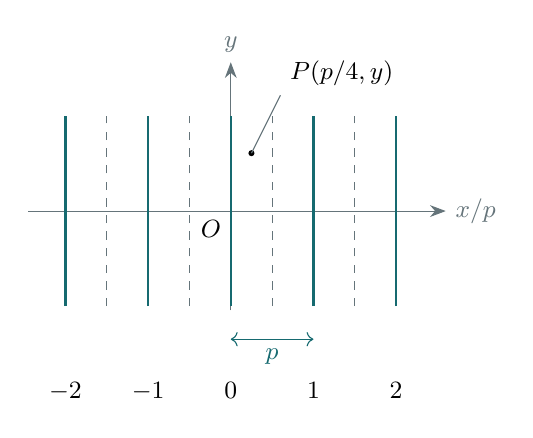
\begin{tikzpicture}
\begin{scope}[x=1.05cm,y=1.05cm]
\draw[axis](-2.45,0)--(2.6,0)node[right]{$x/p$};
\draw[axis](0,-1.2)--(0,1.8)node[above]{$y$};
\foreach \x in{-2,-1,0,1,2}{\draw[traj](\x,-1.15)--(\x,1.15);\node[below]at(\x,-1.95){$\x$};}
\foreach \x in{-1.5,-.5,.5,1.5}{\draw[guide](\x,-1.15)--(\x,1.15);}
\draw[<->,thin,color=accent](0,-1.55)--(1,-1.55)node[midway,below]{$p$};
\fill(.25,.7)circle[radius=1.1pt];\draw[thin,color=muted](.25,.7)--(.6,1.4);
\node[above right]at(.6,1.4){$P(p/4,y)$};
\node[below left]at(0,0){$O$};
\end{scope}
\end{tikzpicture}
\figcaption{解图光2.6C\quad $\delta_0=0$时实线为亮纹、虚线为暗纹，各线平行$y$轴}
\end{minipage}\end{center}

与位置无关的相位$\delta_0$只平移条纹，不改间距和反衬度。当$\theta\to0$时，间距趋于无穷，有限屏幕上可能看不到一次完整明暗变化；$\theta=0$时两波完全共线，屏上强度处处相同，此时不能再把空间条纹的实测反衬度称为$4/5$。$4/5$仍是扫描两束相对相位时的调制度。

在$0<\theta<\pi$内，
\[
\frac{\mathrm dp}{\mathrm d\theta}
=-\frac{\lambda\cos(\theta/2)}{4\sin^2(\theta/2)}<0,
\qquad p\simeq\frac{\lambda}{\theta}\quad(\theta\ll1).
\]
解图光2.6D的单调下降曲线对应上述导数。若屏沿$x$的有效宽度为$W$，
覆盖一个完整周期需$W\geq p$。
只取一对相邻亮暗极值时，合适位置的半周期区间可以足够：
$\delta_0=0$时闭区间$[0,p/2]$同时含亮峰和暗谷，开区间$(0,p/2)$却排除两端极值；
而$\delta_0=\pi/2$时，同一闭区间只含暗谷，未取到亮峰。
一般地，令$\varphi=\delta_0/(2\pi)$，对开屏区$a<x<b$，须同时存在整数$m,n$使
\[
\frac ap+\varphi<m<\frac bp+\varphi,\qquad
\frac ap+\varphi-\frac12<n<\frac bp+\varphi-\frac12.
\]
两式分别保证亮峰$x_m=p(m-\varphi)$与暗谷$x_n=p(n+1/2-\varphi)$在屏内；
闭边界将对应严格不等号改为非严格不等号。
严格$\theta=0$时$\Delta\boldsymbol k=0$，
$I=I_s(5+4\cos\delta_0)$在屏上均匀；调节$\delta_0$仍可在
$I_s$与$9I_s$间变化，但这属于相位扫描。有限光束还须在所讨论屏区真实重叠，
本题平面波模型没有额外给出光束孔径。
\begin{center}\begin{minipage}{.97\linewidth}\centering
\begin{tikzpicture}
\begin{scope}[x=1.7cm,y=.19cm]
\draw[axis](0,0)--(3.3,0)node[right]{$\theta/\mathrm{rad}$};
\draw[axis](0,0)--(0,14)node[above]{$p/\lambda$};
\draw[traj]plot coordinates {(0.0800000000,12.5033339557) (0.0965000000,10.3667162262) (0.1130000000,8.8542676096) (0.1295000000,7.7274061958) (0.1460000000,6.8554021861) (0.1625000000,6.1606222056) (0.1790000000,5.5940574880) (0.1955000000,5.1232444372) (0.2120000000,4.7258260585) (0.2285000000,4.3859029671) (0.2450000000,4.0918588867) (0.2615000000,3.8350093823) (0.2780000000,3.6087317990) (0.2945000000,3.4078876837) (0.3110000000,3.2284290662) (0.3275000000,3.0671237572) (0.3440000000,2.9213597033) (0.3605000000,2.7890030696) (0.3770000000,2.6682935899) (0.3935000000,2.5577662452) (0.4100000000,2.4561918545) (0.4265000000,2.3625314555) (0.4430000000,2.2759008800) (0.4595000000,2.1955429618) (0.4760000000,2.1208055248) (0.4925000000,2.0511237960) (0.5090000000,1.9860062388) (0.5255000000,1.9250230555) (0.5420000000,1.8677967899) (0.5585000000,1.8139945954) (0.5750000000,1.7633218346) (0.5915000000,1.7155167501) (0.6080000000,1.6703460031) (0.6245000000,1.6276009189) (0.6410000000,1.5870943129) (0.6575000000,1.5486577936) (0.6740000000,1.5121394630) (0.6905000000,1.4774019455) (0.7070000000,1.4443206935) (0.7235000000,1.4127825244) (0.7400000000,1.3826843542) (0.7565000000,1.3539320954) (0.7730000000,1.3264396976) (0.7895000000,1.3001283072) (0.8060000000,1.2749255312) (0.8225000000,1.2507647886) (0.8390000000,1.2275847396) (0.8555000000,1.2053287797) (0.8720000000,1.1839445921) (0.8885000000,1.1633837493) (0.9050000000,1.1436013587) (0.9215000000,1.1245557463) (0.9380000000,1.1062081733) (0.9545000000,1.0885225828) (0.9710000000,1.0714653718) (0.9875000000,1.0550051861) (1.0040000000,1.0391127360) (1.0205000000,1.0237606288) (1.0370000000,1.0089232185) (1.0535000000,0.9945764685) (1.0700000000,0.9806978280) (1.0865000000,0.9672661192) (1.1030000000,0.9542614341) (1.1195000000,0.9416650418) (1.1360000000,0.9294593022) (1.1525000000,0.9176275887) (1.1690000000,0.9061542160) (1.1855000000,0.8950243754) (1.2020000000,0.8842240739) (1.2185000000,0.8737400797) (1.2350000000,0.8635598707) (1.2515000000,0.8536715885) (1.2680000000,0.8440639946) (1.2845000000,0.8347264310) (1.3010000000,0.8256487835) (1.3175000000,0.8168214471) (1.3340000000,0.8082352955) (1.3505000000,0.7998816509) (1.3670000000,0.7917522577) (1.3835000000,0.7838392570) (1.4000000000,0.7761351635) (1.4165000000,0.7686328435) (1.4330000000,0.7613254949) (1.4495000000,0.7542066285) (1.4660000000,0.7472700499) (1.4825000000,0.7405098440) (1.4990000000,0.7339203586) (1.5155000000,0.7274961912) (1.5320000000,0.7212321749) (1.5485000000,0.7151233660) (1.5650000000,0.7091650327) (1.5815000000,0.7033526435) (1.5980000000,0.6976818572) (1.6145000000,0.6921485135) (1.6310000000,0.6867486232) (1.6475000000,0.6814783604) (1.6640000000,0.6763340541) (1.6805000000,0.6713121806) (1.6970000000,0.6664093566) (1.7135000000,0.6616223323) (1.7300000000,0.6569479852) (1.7465000000,0.6523833142) (1.7630000000,0.6479254337) (1.7795000000,0.6435715687) (1.7960000000,0.6393190494) (1.8125000000,0.6351653068) (1.8290000000,0.6311078678) (1.8455000000,0.6271443516) (1.8620000000,0.6232724648) (1.8785000000,0.6194899986) (1.8950000000,0.6157948244) (1.9115000000,0.6121848908) (1.9280000000,0.6086582202) (1.9445000000,0.6052129058) (1.9610000000,0.6018471088) (1.9775000000,0.5985590553) (1.9940000000,0.5953470340) (2.0105000000,0.5922093937) (2.0270000000,0.5891445406) (2.0435000000,0.5861509365) (2.0600000000,0.5832270962) (2.0765000000,0.5803715857) (2.0930000000,0.5775830205) (2.1095000000,0.5748600632) (2.1260000000,0.5722014221) (2.1425000000,0.5696058496) (2.1590000000,0.5670721402) (2.1755000000,0.5645991294) (2.1920000000,0.5621856920) (2.2085000000,0.5598307409) (2.2250000000,0.5575332255) (2.2415000000,0.5552921306) (2.2580000000,0.5531064754) (2.2745000000,0.5509753119) (2.2910000000,0.5488977242) (2.3075000000,0.5468728273) (2.3240000000,0.5448997659) (2.3405000000,0.5429777140) (2.3570000000,0.5411058732) (2.3735000000,0.5392834726) (2.3900000000,0.5375097674) (2.4065000000,0.5357840385) (2.4230000000,0.5341055914) (2.4395000000,0.5324737557) (2.4560000000,0.5308878843) (2.4725000000,0.5293473527) (2.4890000000,0.5278515587) (2.5055000000,0.5263999213) (2.5220000000,0.5249918802) (2.5385000000,0.5236268957) (2.5550000000,0.5223044478) (2.5715000000,0.5210240355) (2.5880000000,0.5197851767) (2.6045000000,0.5185874078) (2.6210000000,0.5174302828) (2.6375000000,0.5163133733) (2.6540000000,0.5152362677) (2.6705000000,0.5141985714) (2.6870000000,0.5131999058) (2.7035000000,0.5122399085) (2.7200000000,0.5113182324) (2.7365000000,0.5104345459) (2.7530000000,0.5095885325) (2.7695000000,0.5087798902) (2.7860000000,0.5080083316) (2.8025000000,0.5072735834) (2.8190000000,0.5065753863) (2.8355000000,0.5059134947) (2.8520000000,0.5052876766) (2.8685000000,0.5046977132) (2.8850000000,0.5041433989) (2.9015000000,0.5036245410) (2.9180000000,0.5031409597) (2.9345000000,0.5026924877) (2.9510000000,0.5022789701) (2.9675000000,0.5019002646) (2.9840000000,0.5015562411) (3.0005000000,0.5012467813) (3.0170000000,0.5009717794) (3.0335000000,0.5007311412) (3.0500000000,0.5005247845)};
\foreach \x in{1,2,3}{\node[below]at(\x,0){$\x$};}
\node[left]at(0,1){$1$};\node[left]at(0,10){$10$};
\node[align=center]at(1.85,10){$\theta\downarrow0$时$p\uparrow\infty$\\曲线取$0.08\leq\theta\leq3.05$};
\end{scope}
\end{tikzpicture}
\figcaption{解图光2.6D\quad 在$0<\theta<\pi$内夹角增大，空间周期单调减小}
\end{minipage}\end{center}


\Needspace{13\baselineskip}

\pdfbookmark[2]{第 7 题 双棱镜的最佳观察距离}{q7}

\section*{第 7 题\quad 双棱镜的最佳观察距离}\label{q:7}

波长$\lambda=632.8\,\mathrm{nm}$的平行光垂直照到菲涅耳双棱镜上。每个半棱镜的折射顶角为$\alpha=3'30''$，总通光宽度$W=4.0\,\mathrm{cm}$，折射率$n=1.5$。求屏距$L$为何值时共同照明区及条纹数最大，何时共同照明区消失，并计算最大条纹覆盖数和对称区内实际亮纹条数。两半等厚、同相，忽略边缘衍射。

\begin{center}\begin{minipage}{.98\linewidth}\centering
\begin{tikzpicture}[x=0.160000000cm,y=.12cm]
\draw[axis](-4.000000000000,0.000000000000)--(43.860045903905,0.000000000000)node[right]{$z/\mathrm m$};
\draw[object](0.000000000000,-20.000000000000)--(0.000000000000,20.000000000000);
\draw[motion](-3.000000000000,20.000000000000)--(0.000000000000,20.000000000000);
\draw[motion](-3.000000000000,0.000000000000)--(0.000000000000,0.000000000000);
\draw[motion](-3.000000000000,-20.000000000000)--(0.000000000000,-20.000000000000);
\draw[motion](0.000000000000,20.000000000000)--(40.860045903905,-0.800000000000);
\draw[motion](0.000000000000,0.000000000000)--(40.860045903905,-20.800000000000);
\draw[force](0.000000000000,0.000000000000)--(40.860045903905,20.800000000000);
\draw[force](0.000000000000,-20.000000000000)--(40.860045903905,0.800000000000);
\draw[object](19.644252838416,-24.000000000000)--(19.644252838416,24.000000000000);
\node[above]at(19.644252838416,24.000000000000){屏};
\node[below]at(0.000000000000,-24.000000000000){偏折等效面};
\node[above,align=center]at(-3.200000000000,24.000000000000){$y/\mathrm{mm}$\\横向放大};
\draw[guide](39.288505676831,-24.000000000000)--(39.288505676831,24.000000000000);
\node[above]at(39.288505676831,24.000000000000){$L_0$};
\node[below right]at(19.644252838416,-24.000000000000){$L_*$};
\node[below right]at(39.288505676831,-24.000000000000){$39.2885\,\mathrm m$};
\node[below left]at(-2.000000000000,20.000000000000){$20$};
\node[above left]at(-2.000000000000,-20.000000000000){$-20$};
\end{tikzpicture}
\figcaption{图光2.7\quad 两束的四条边界；轴向米、横向毫米}
\end{minipage}\end{center}

图用零厚度棱镜等效面表示偏折；横向放大，$z$用米、$y$用毫米。请区分连续覆盖数最大时的屏距和整数亮纹数达到最大值的屏距范围。

\Needspace{6\baselineskip}\subsection*{解答}


解图光2.7A中，两个半棱镜分别将上、下半光束向轴线偏转$\eta$。入口正入射，出口应用折射定律，
\[
\eta=\arcsin(n\sin\alpha)-\alpha
\simeq(n-1)\alpha,\qquad
\alpha=1.018109\times10^{-3}\,\mathrm{rad}.
\]
于是$\eta\simeq5.09054\times10^{-4}\,\mathrm{rad}$。两束夹全角$2\eta$，由屏内波矢差得
\[
p=\frac{\lambda}{2\sin\eta}\simeq0.62154\,\mathrm{mm}.
\]
\begin{center}\begin{minipage}{.98\linewidth}\centering
\begin{tikzpicture}[x=0.160000000cm,y=.12cm]
\fill[color=accent!12](0.000000000000,0.000000000000)--(19.644252838416,10.000000000000)--(39.288505676831,0.000000000000)--(19.644252838416,-10.000000000000)--cycle;
\draw[axis](-4.000000000000,0.000000000000)--(43.860045903905,0.000000000000)node[right]{$z/\mathrm m$};
\draw[object](0.000000000000,-20.000000000000)--(0.000000000000,20.000000000000);
\draw[motion](-3.000000000000,20.000000000000)--(0.000000000000,20.000000000000);
\draw[motion](-3.000000000000,0.000000000000)--(0.000000000000,0.000000000000);
\draw[motion](-3.000000000000,-20.000000000000)--(0.000000000000,-20.000000000000);
\draw[motion](0.000000000000,20.000000000000)--(40.860045903905,-0.800000000000);
\draw[motion](0.000000000000,0.000000000000)--(40.860045903905,-20.800000000000);
\draw[force](0.000000000000,0.000000000000)--(40.860045903905,20.800000000000);
\draw[force](0.000000000000,-20.000000000000)--(40.860045903905,0.800000000000);
\draw[object](19.644252838416,-24.000000000000)--(19.644252838416,24.000000000000);
\node[above]at(19.644252838416,24.000000000000){屏};
\node[below]at(0.000000000000,-24.000000000000){偏折等效面};
\node[above,align=center]at(-3.200000000000,24.000000000000){$y/\mathrm{mm}$\\横向放大};
\draw[guide](39.288505676831,-24.000000000000)--(39.288505676831,24.000000000000);
\node[above]at(39.288505676831,24.000000000000){$L_0$};
\node[below right]at(19.644252838416,-24.000000000000){$L_*$};
\node[below right]at(39.288505676831,-24.000000000000){$39.2885\,\mathrm m$};
\draw[<->,thin,color=muted](21.644252838416,-10.000000000000)--(21.644252838416,10.000000000000);
\node[above]at(19.644252838416,28.000000000000){$W_c=20\,\mathrm{mm}$};
\end{tikzpicture}
\figcaption{解图光2.7A\quad 相反倾斜光束的共同区与最佳屏}
\end{minipage}\end{center}
令$a=L\tan\eta$，上半束在屏上的区间为$[-a,W/2-a]$，下半束为$[-W/2+a,a]$，所以共同宽度为
\[
W_c(L)=
\begin{cases}
2a,&0\le a\le W/4,\\
W-2a,&W/4\le a\le W/2,\\
0,&a\ge W/2.
\end{cases}
\]
随$L$增加，两束先靠近、再错开，交集宽度先增后减。峰值发生在$a=W/4$：
\[
\boxed{L_*=\frac{W}{4\tan\eta}\simeq19.64\,\mathrm m,\quad
W_{c,\max}=W/2=20.0\,\mathrm{mm}.}
\]
共同照明区在
\[
\boxed{L\ge L_0=\frac{W}{2\tan\eta}\simeq39.29\,\mathrm m}
\]
消失。$L=0$时也只有分界线处接触，没有有限宽重叠。

最大覆盖条纹间隔数为$W_{c,\max}/p\simeq32.18$。若中央同相，$|m|p<W/4$，得到$m=-16,\ldots,16$，共33条亮纹。若把两半的附加相位改变，宽度和间距不变，实际亮纹数可能相差一条。解图光2.7B 中，随屏距增大，左右两束的公共照明宽度先增大，再减小。两条直线段的交点给出最大值 $W/2$。
\begin{center}\begin{minipage}{.98\linewidth}\centering
\begin{tikzpicture}[x=1cm,y=1cm]
\begin{scope}[x=12cm,y=6cm]
\draw[axis](0,0)--(.62,0);
\draw[axis](0,0)--(0,.62)node[above]{$W_c/W$};
\draw[traj]plot coordinates {(0,0)(.25,.5)(.5,0)(.57,0)};
\node[below left]at(0,0){$0$};\node[below]at(.25,0){$1/4$};\node[below]at(.5,0){$1/2$};
\node[left]at(0,.5){$1/2$};\node[above]at(.25,.5){$L_*$};
\node[below]at(.32,-.13){$u=L\tan\eta/W$};
\end{scope}
\begin{scope}[shift={(10cm,.65cm)},x=.14cm,y=.7cm]
\draw[line width=2pt,color=accent](-10,2)--(10,2);\draw[line width=2pt,color=warm](-10,1)--(10,1);
\draw[line width=2pt,color=accent](-10,0)--(10,0);
\node[left]at(-11,2){上束};\node[left]at(-11,1){下束};\node[left]at(-11,0){共同区};
\node[above]at(-10,2){$-10$};\node[above]at(10,2){$10$};
\node[below]at(0,-.1){$y/\mathrm{mm}$，$L=L_*$};
\end{scope}
\end{tikzpicture}
\figcaption{解图光2.7B\quad 宽度分段函数和最佳屏上的区间}
\end{minipage}\end{center}

解图光2.7C画出上半棱镜出口处的波矢分量。记真空波数$k_0=2\pi/\lambda$，传播轴沿$+z$，出口外法线与$+z$夹角为$+\alpha$。取正交单位方向
\[
\widehat{\boldsymbol n}=(\cos\alpha,\sin\alpha),\qquad
\widehat{\boldsymbol t}=(-\sin\alpha,\cos\alpha),
\]
分量次序是$(z,y)$。入射光在入口正入射，在玻璃内仍沿$+z$；它在出口处的法向、切向分量分别为$nk_0\cos\alpha$和$-nk_0\sin\alpha$。界面相位连续要求切向波矢相等，故出射角$\beta$满足$\sin\beta=n\sin\alpha$。再投回全局方向，
\[
\frac{\boldsymbol k_+}{k_0}
=\cos\beta\,\widehat{\boldsymbol n}-\sin\beta\,\widehat{\boldsymbol t}
=(\cos\eta,-\sin\eta),\qquad\eta=\beta-\alpha>0.
\]
上束向下倾斜，下束的$y$分量相反，均向轴线偏转。解图光2.7C的横坐标额外除以$\alpha$以显示小分量，箭头在纸上的夹角不能当作实际折射角。

\begin{center}\begin{minipage}{.98\linewidth}\centering
\begin{tikzpicture}[x=2cm,y=1.8cm]
\draw[axis](-1.9,0)--(.5,0)node[right]{$k_t/(k_0\alpha)$};
\draw[axis](0,0)--(0,1.85)node[above]{$k_n/k_0$};
\draw[motion](0,0)--(-1.499999740864,1.499999222591);
\draw[force](0,0)--(-1.499999740864,0.999998833886);
\draw[guide](-1.499999740864,0.000000000000)--(-1.499999740864,1.499999222591);
\node[above left]at(-1.499999740864,1.499999222591){玻璃内};
\node[below left]at(-1.499999740864,0.999998833886){空气中};
\node[below]at(-1.499999740864,-0.100000000000){$-n\sin\alpha/\alpha$};
\node[below right]at(0,0){$0$};
\node[right,align=left]at(.55,1.1){上半出口\\$\beta=\alpha+\eta$\\$\sin\beta=n\sin\alpha$};
\end{tikzpicture}
\figcaption{解图光2.7C\quad 出口正交分量中的切向波矢连续}
\end{minipage}\end{center}

角度换算为$3'30''=210''=\tfrac7{120}^{\circ}=7\pi/21600$弧度。取$n=1.5$，精确折射式在薄棱镜模型中给出
\[
\eta=5.09054695\times10^{-4}\,\mathrm{rad},\quad
p=0.62154424\,\mathrm{mm},\quad
L_*=19.64425284\,\mathrm m,\quad L_0=39.28850568\,\mathrm m.
\]
小角近似的误差可以分开检查：
\[
\eta=(n-1)\alpha+\frac{n(n^2-1)}6\alpha^3+O(\alpha^5),
\qquad \tan\eta=\eta+\frac{\eta^3}3+O(\eta^5).
\]
此处棱镜偏角线性近似的相对误差约$6.48\times10^{-7}$；$\tan\eta$与$\eta$的相对差约$8.64\times10^{-8}$，因而前面的有效数字足够。出口须有$n\sin\alpha<1$；等于1时为沿界面的临界掠射方向，大于1时全反射，这两种边界情形都不能套用本题的透射光束图形。

条纹间距不随屏距变化，也可直接从波矢求出。两束在同一$z$平面的共同区内，相位差的空间项为
\[
\Psi(y)=(\boldsymbol k_--\boldsymbol k_+)\!\cdot\!(z,y)
=2k_0y\sin\eta,\qquad
\Psi(y+p)-\Psi(y)=2\pi.
\]
两束的$z$分量相同，故相位差中没有$L$项；共同区却随$L$改变，不能由相位公式判断那里是否有光。解图光2.7A、B以$z$米、$y$毫米或各自标出的无量纲坐标画出几何边界。对厚度忽略的等效面，上束在$0\le y\le W/2$入射，下束在$-W/2\le y\le0$入射，每半束横向宽度是$W/2$。在$L_*$处，两个区间都变成$[-W/4,W/4]$，因此最大共同全宽是$W/2=20.0\,\mathrm{mm}$；代入$2L_*\tan\eta$也得到同一数值。

解图光2.7D逐一画出最大共同区内的相长级次。中心同相时$y_m=mp$；边缘按题设的几何光学模型取开区间，
\[
|m|<\frac{W}{4p}=16.08895932,
\qquad m=-16,\ldots,16,
\qquad N_{\max}=33.
\]
全宽与间距的比$20.0/.62154424=32.17791865$是连续跨度，不是亮纹条数。

\begin{center}\begin{minipage}{.98\linewidth}\centering
\begin{tikzpicture}[x=0.390000000cm,y=.65cm]
\fill[color=accent!10](-10.000000000000,0.000000000000)rectangle(10.000000000000,1.100000000000);
\draw[axis](-11.000000000000,0.000000000000)--(12.000000000000,0.000000000000)node[right]{$y/\mathrm{mm}$};
\draw[color=accent,thick](-9.944707845439,0.150000000000)--(-9.944707845439,0.900000000000);
\draw[color=accent,thick](-9.323163605099,0.150000000000)--(-9.323163605099,0.900000000000);
\draw[color=accent,thick](-8.701619364759,0.150000000000)--(-8.701619364759,0.900000000000);
\draw[color=accent,thick](-8.080075124419,0.150000000000)--(-8.080075124419,0.900000000000);
\draw[color=accent,thick](-7.458530884079,0.150000000000)--(-7.458530884079,0.900000000000);
\draw[color=accent,thick](-6.836986643739,0.150000000000)--(-6.836986643739,0.900000000000);
\draw[color=accent,thick](-6.215442403399,0.150000000000)--(-6.215442403399,0.900000000000);
\draw[color=accent,thick](-5.593898163059,0.150000000000)--(-5.593898163059,0.900000000000);
\draw[color=accent,thick](-4.972353922719,0.150000000000)--(-4.972353922719,0.900000000000);
\draw[color=accent,thick](-4.350809682379,0.150000000000)--(-4.350809682379,0.900000000000);
\draw[color=accent,thick](-3.729265442040,0.150000000000)--(-3.729265442040,0.900000000000);
\draw[color=accent,thick](-3.107721201700,0.150000000000)--(-3.107721201700,0.900000000000);
\draw[color=accent,thick](-2.486176961360,0.150000000000)--(-2.486176961360,0.900000000000);
\draw[color=accent,thick](-1.864632721020,0.150000000000)--(-1.864632721020,0.900000000000);
\draw[color=accent,thick](-1.243088480680,0.150000000000)--(-1.243088480680,0.900000000000);
\draw[color=accent,thick](-0.621544240340,0.150000000000)--(-0.621544240340,0.900000000000);
\draw[color=accent,thick](0.000000000000,0.150000000000)--(0.000000000000,0.900000000000);
\draw[color=accent,thick](0.621544240340,0.150000000000)--(0.621544240340,0.900000000000);
\draw[color=accent,thick](1.243088480680,0.150000000000)--(1.243088480680,0.900000000000);
\draw[color=accent,thick](1.864632721020,0.150000000000)--(1.864632721020,0.900000000000);
\draw[color=accent,thick](2.486176961360,0.150000000000)--(2.486176961360,0.900000000000);
\draw[color=accent,thick](3.107721201700,0.150000000000)--(3.107721201700,0.900000000000);
\draw[color=accent,thick](3.729265442040,0.150000000000)--(3.729265442040,0.900000000000);
\draw[color=accent,thick](4.350809682379,0.150000000000)--(4.350809682379,0.900000000000);
\draw[color=accent,thick](4.972353922719,0.150000000000)--(4.972353922719,0.900000000000);
\draw[color=accent,thick](5.593898163059,0.150000000000)--(5.593898163059,0.900000000000);
\draw[color=accent,thick](6.215442403399,0.150000000000)--(6.215442403399,0.900000000000);
\draw[color=accent,thick](6.836986643739,0.150000000000)--(6.836986643739,0.900000000000);
\draw[color=accent,thick](7.458530884079,0.150000000000)--(7.458530884079,0.900000000000);
\draw[color=accent,thick](8.080075124419,0.150000000000)--(8.080075124419,0.900000000000);
\draw[color=accent,thick](8.701619364759,0.150000000000)--(8.701619364759,0.900000000000);
\draw[color=accent,thick](9.323163605099,0.150000000000)--(9.323163605099,0.900000000000);
\draw[color=accent,thick](9.944707845439,0.150000000000)--(9.944707845439,0.900000000000);
\node[above]at(-10.000000000000,1.100000000000){$-10$};
\node[above]at(10.000000000000,1.100000000000){$10$};
\node[below]at(0,0){$0$};
\node[above]at(0,1.3){$33$条亮纹};
\end{tikzpicture}
\figcaption{解图光2.7D\quad 20毫米窗口内的33个整数级次}
\end{minipage}\end{center}

整数最大条数不只在$L_*$取得。令共同半宽$h=W_c/2=\min(a,W/2-a)$，在$0<a<W/2$内至少容纳$m=\pm16$须有$16p<h$；由于$h\le10\,\mathrm{mm}<17p$，这也恰是达到33条的充分条件：
\[
16p<L\tan\eta<\frac W2-16p,
\qquad
19.53563553<L<19.75287014\quad(\mathrm m).
\]
两个端点处$m=\pm16$恰落在几何边缘，按开区间只剩31条；若连理想边缘也计入，则端点为33条。$L_*$仍是共同宽度和连续覆盖数的唯一最大点。$L=0$或$L=L_0$时两束只在一条边界线上相接，$L>L_0$时完全分开，均没有有限宽条纹区；几何相切点不计为具有宽度的一条亮纹。

以上把两半棱镜作为零厚度的偏折等效面，忽略有限厚度造成的微小横移和边缘衍射；波长在空气中取题给数值，入射光在总通光宽度内近似均匀且两束同偏振、相干。图中横向放大、轴向单位为米而横向为毫米，实际光线的斜率仍由$\pm\tan\eta$决定，不可用纸面夹角代替它。


\Needspace{13\baselineskip}

\pdfbookmark[2]{第 8 题 三平面波的三种组合}{q8}

\section*{第 8 题\quad 三平面波的三种组合}\label{q:8}

三束同频、同偏振平面波在$xz$平面内传播，波长均为$\lambda$，波矢$\boldsymbol k_2$沿$+z$，$\boldsymbol k_1,\boldsymbol k_3$分别与$+z$成$\pm\theta$。振幅依次为$A_0,2A_0,A_0$，在原点的相位相同。屏为$z=0$。分别求三束同时存在、仅保留第1与3束、仅保留第1与2束时的强度分布、反衬度和条纹间距，并比较图样。

\begin{center}\begin{minipage}{.98\linewidth}\centering
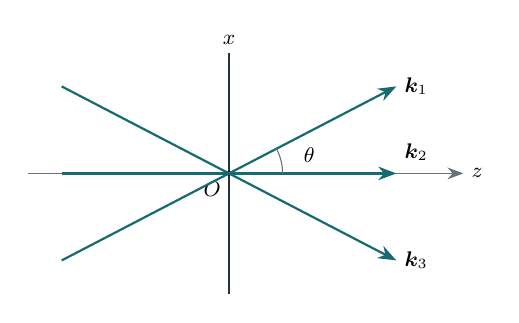
\begin{tikzpicture}[scale=.85,transform shape]
\draw[axis] (-3.00000,0.00000)--(3.50000,0.00000);\draw[object] (0.00000,-1.80000)--(0.00000,1.80000);\fill (0.00000,0.00000) circle(.035);\node[below left] at (0.00000,0.00000) {$O$};\node[above] at (0.00000,1.80000) {$x$};\node[right] at (3.50000,0.00000) {$z$};\draw[motion] (-2.50000,-1.30000)--(2.50000,1.30000);\node[right] at (2.50000,1.30000) {$\boldsymbol k_1$};\draw[motion] (-2.50000,0.00000)--(2.50000,0.00000);\node[above right,yshift=2pt] at (2.50000,0.00000) {$\boldsymbol k_2$};\draw[motion] (-2.50000,1.30000)--(2.50000,-1.30000);\node[right] at (2.50000,-1.30000) {$\boldsymbol k_3$};\draw[thin,color=muted] (.8,0) arc[start angle=0,end angle=27.47443,radius=.8];\node[] at (1.20000,0.28000) {$\theta$};
\end{tikzpicture}
\figcaption{图光2.8\quad 传播平面与$z=0$接收屏}
\end{minipage}\end{center}

取$A_0>0$，$0<\theta<\pi/2$；共同线偏振沿$y$方向，垂直于传播平面。强度按同一比例常数乘以合振幅模平方定义。图中屏为$x$轴所在的$z=0$平面截线。

\Needspace{6\baselineskip}\subsection*{解答}


取$\boldsymbol r=x\boldsymbol i+y\boldsymbol j+z\boldsymbol k$，$k=2\pi/\lambda$。图光2.8中第1束的$x$分量为正，第3束为负：
\[
\boldsymbol k_1=k(\sin\theta\,\boldsymbol i+\cos\theta\,\boldsymbol k),\quad
\boldsymbol k_2=k\boldsymbol k,\quad
\boldsymbol k_3=k(-\sin\theta\,\boldsymbol i+\cos\theta\,\boldsymbol k).
\]
三个方向与$y$轴的方向余弦均为零。分别与$\boldsymbol r$作内积，得到
\[
\begin{aligned}
\boldsymbol k_1\cdot\boldsymbol r
 &=k(x\cos\alpha_1+y\cos\beta_1+z\cos\gamma_1)
 =k(x\sin\theta+z\cos\theta),\\
\boldsymbol k_2\cdot\boldsymbol r
 &=k(x\cos\alpha_2+y\cos\beta_2+z\cos\gamma_2)=kz,\\
\boldsymbol k_3\cdot\boldsymbol r
 &=k(x\cos\alpha_3+y\cos\beta_3+z\cos\gamma_3)
 =k(-x\sin\theta+z\cos\theta).
\end{aligned}
\]
三波的时间振动式是
\[
\begin{aligned}
u_1(\boldsymbol r,t)&=A_0\cos(\omega t-\boldsymbol k_1\cdot\boldsymbol r),\\
u_2(\boldsymbol r,t)&=2A_0\cos(\omega t-\boldsymbol k_2\cdot\boldsymbol r),\\
u_3(\boldsymbol r,t)&=A_0\cos(\omega t-\boldsymbol k_3\cdot\boldsymbol r).
\end{aligned}
\]
在图光2.8的屏截线上，$z=0$。令$q=k\sin\theta$，三相位依次为$qx,0,-qx$，于是
\[
u_1(x,t)=A_0\cos(\omega t-qx),\quad
u_2(x,t)=2A_0\cos\omega t,\quad
u_3(x,t)=A_0\cos(\omega t+qx).
\]
以下取$u_j=\Re(\widetilde E_j e^{-i\omega t})$；以同一强度比例常数$C$记$I_s=CA_0^2$，于是$I=C|\widetilde E|^2$。时间平均中的常数已含在$C$内。三束同频、沿$y$同向偏振，且相位差稳定，时间平均后仍保留干涉交叉项。

图光2.8中令$q=2\pi\sin\theta/\lambda$，以单束振幅$A_0$对应的强度为$I_s$。屏上三束的复振幅可取
\[
\widetilde E_1=A_0e^{iqx},\qquad
\widetilde E_2=2A_0,\qquad
\widetilde E_3=A_0e^{-iqx}.
\]
解图光2.8A中第1、3束相量关于实轴对称，它们的虚部抵消；但仅有第1、2束时，没有第3束去抵消虚部。
\begin{center}\begin{minipage}{.98\linewidth}\centering
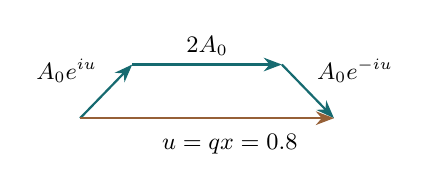
\begin{tikzpicture}[scale=.95,transform shape]
\draw[motion] (0.00000,0.00000)--(0.69671,0.71736);
\draw[motion] (0.69671,0.71736)--(2.69671,0.71736);
\draw[motion] (2.69671,0.71736)--(3.39341,0.00000);\draw[force] (0.00000,0.00000)--(3.39341,0.00000);\node[above left] at (0.34835,0.35868) {$A_0e^{iu}$};\node[above] at (1.69671,0.71736) {$2A_0$};\node[above right] at (3.04506,0.35868) {$A_0e^{-iu}$};\node[above] at (2.00000,-0.60000) {$u=qx=0.8$};
\end{tikzpicture}
\figcaption{解图光2.8A\quad 对称相量的虚部抵消；删去一束后须重算模平方}
\end{minipage}\end{center}
三束同时存在时，
\[
\widetilde E=2A_0(1+\cos qx),\quad
\boxed{I_{123}=4I_s(1+\cos qx)^2}.
\]
极大为$16I_s$，发生于$qx=2m\pi$；极小为零，发生于$qx=(2m+1)\pi$。因此$\gamma_{123}=1$，相邻亮纹间距$p_{123}=2\pi/q=\lambda/\sin\theta$。


对解图光2.8A，也可先用时间振动式相加：
\[
u_1+u_3=2A_0\cos qx\cos\omega t,\qquad
u_1+u_2+u_3=2A_0(1+\cos qx)\cos\omega t.
\]
因为$1+\cos qx\ge0$，三束的振幅就是$A=2A_0(1+\cos qx)$。展开平方，或先用指数和化余弦，分别得到
\[
\begin{aligned}
I_{123}/I_s&=4(1+2\cos qx+\cos^2qx),\\
\widetilde E/A_0&=2+e^{iqx}+e^{-iqx}=2+2\cos qx.
\end{aligned}
\]
时间振动相加、图A的相量投影与复数相加都得到上述振幅。令$u=qx$，极大条件$u=2m\pi$给出$x_m=m\lambda/\sin\theta$，代入展开式得$4I_s(1+2+1)=16I_s$；极小条件$u=(2m+1)\pi$给出$x_{m,\min}=(m+\tfrac12)\lambda/\sin\theta$，代入得$4I_s(1-2+1)=0$。这里及下文$m\in\mathbb Z$。相邻极大位置相减给出$p_{123}$，反衬度按
\[
\gamma=\frac{I_{\max}-I_{\min}}{I_{\max}+I_{\min}}
\]
计算；分母是强度之和。

仅第1、3束存在时，
\[
\widetilde E=2A_0\cos qx,\qquad
\boxed{I_{13}=4I_s\cos^2qx}.
\]
极大为$4I_s$，发生于$qx=m\pi$；极小为零，故$\gamma_{13}=1$，间距$p_{13}=\pi/q=\lambda/(2\sin\theta)$。比三束图样加密一倍。


第1、3束的合相量$2A_0\cos u$可为负；物理振幅为$2A_0|\cos u|$，负号只是时间振动相位改变$\pi$。亮纹$x_m=m\lambda/(2\sin\theta)$，暗纹$x_{m,\min}=(m+\tfrac12)\lambda/(2\sin\theta)$。两组位置都由强度的平方求出，不能把合相量的有符号周期当作强度周期。

仅第1、2束存在时，应保留完整复数：
\[
I_{12}=I_s|2+e^{iqx}|^2
=I_s[(2+\cos qx)^2+\sin^2qx]
=\boxed{I_s(5+4\cos qx)}.
\]
极大$9I_s$、极小$I_s$，故$\gamma_{12}=4/5$，$p_{12}=\lambda/\sin\theta$。若把振幅误写成$A_0(2+\cos qx)$再平方，虽然恰好得到相同的极大、极小，却会算错中间每一点的强度。


解图光2.8C取$u=\pi/2$，实部为$2A_0$，虚部为$A_0$，合振幅是$\sqrt5A_0$。一般地，
\[
\begin{aligned}
u_1+u_2
 &=A_0[(2+\cos u)\cos\omega t+\sin u\sin\omega t],\\
A_{12}
 &=A_0\sqrt{(2+\cos u)^2+\sin^2u}
 =A_0\sqrt{5+4\cos u}.
\end{aligned}
\]
两正交时间分量均须计入。极大仍在$u=2m\pi$，$I_{\max}=I_s(5+4)=9I_s$；极小在$u=(2m+1)\pi$，$I_{\min}=I_s(5-4)=I_s$。因此$\gamma_{12}=(9-1)/(9+1)=0.8$，亮纹$x_m=m\lambda/\sin\theta$。只取同相分量时，少了一项 $I_s\sin^2u$。这项在上述极大、极小处均为零，在其他相位仍要计入。
\begin{center}\begin{minipage}{.98\linewidth}\centering
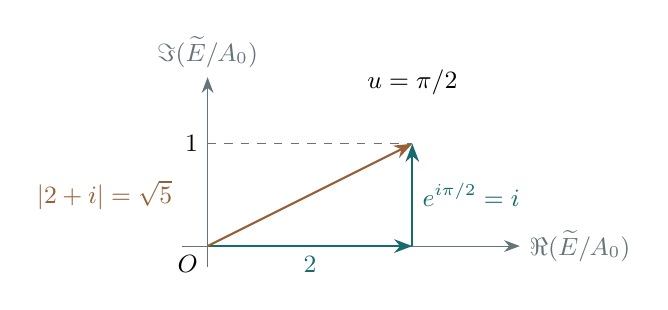
\begin{tikzpicture}[scale=1.3]
\draw[axis] (-.25,0)--(3.05,0) node[right] {$\Re(\widetilde E/A_0)$};
\draw[axis] (0,-.2)--(0,1.65) node[above] {$\Im(\widetilde E/A_0)$};
\draw[motion] (0,0)--(2,0) node[midway,below] {$2$};
\draw[motion] (2,0)--(2,1) node[midway,right] {$e^{i\pi/2}=i$};
\draw[force] (0,0)--(2,1);
\node[left,text=warm] at (-.25,.5) {$|2+i|=\sqrt5$};
\draw[guide] (0,1)--(2,1);
\node[left] at (0,1) {$1$};
\node[below left] at (0,0) {$O$};
\node[above] at (2,1.38) {$u=\pi/2$};
\end{tikzpicture}
\figcaption{解图光2.8C\quad 不对称两束保留虚部}
\end{minipage}\end{center}

解图光2.8B用同一横坐标画三种强度，能看出它们的峰高、周期和暗纹形状均有区别。在$qx=\pi$附近，三束合振幅从二阶项起变化，强度从四阶项起变化；等振幅双束的暗纹强度则从二阶项起变化。两者虽然可见度都为1，暗纹附近的形状仍不同。
\begin{center}\begin{minipage}{.98\linewidth}\centering
\begin{tikzpicture}[scale=.9,transform shape]
\draw[axis] (0.00000,0.00000)--(7.00000,0.00000);\draw[axis] (0.00000,0.00000)--(0.00000,3.00000);\draw[traj] plot coordinates {(0.00000,2.60000) (0.01625,2.59968) (0.03250,2.59872) (0.04875,2.59711) (0.06500,2.59487) (0.08125,2.59199) (0.09750,2.58847) (0.11375,2.58432) (0.13000,2.57954) (0.14625,2.57413) (0.16250,2.56809) (0.17875,2.56143) (0.19500,2.55415) (0.21125,2.54626) (0.22750,2.53776) (0.24375,2.52866) (0.26000,2.51896) (0.27625,2.50867) (0.29250,2.49779) (0.30875,2.48633) (0.32500,2.47430) (0.34125,2.46171) (0.35750,2.44856) (0.37375,2.43486) (0.39000,2.42062) (0.40625,2.40585) (0.42250,2.39056) (0.43875,2.37475) (0.45500,2.35844) (0.47125,2.34163) (0.48750,2.32434) (0.50375,2.30657) (0.52000,2.28834) (0.53625,2.26966) (0.55250,2.25053) (0.56875,2.23098) (0.58500,2.21100) (0.60125,2.19062) (0.61750,2.16985) (0.63375,2.14868) (0.65000,2.12715) (0.66625,2.10526) (0.68250,2.08303) (0.69875,2.06046) (0.71500,2.03757) (0.73125,2.01437) (0.74750,1.99088) (0.76375,1.96711) (0.78000,1.94307) (0.79625,1.91877) (0.81250,1.89424) (0.82875,1.86948) (0.84500,1.84450) (0.86125,1.81933) (0.87750,1.79397) (0.89375,1.76844) (0.91000,1.74275) (0.92625,1.71692) (0.94250,1.69095) (0.95875,1.66487) (0.97500,1.63869) (0.99125,1.61242) (1.00750,1.58607) (1.02375,1.55966) (1.04000,1.53320) (1.05625,1.50670) (1.07250,1.48018) (1.08875,1.45366) (1.10500,1.42714) (1.12125,1.40063) (1.13750,1.37416) (1.15375,1.34773) (1.17000,1.32135) (1.18625,1.29504) (1.20250,1.26881) (1.21875,1.24268) (1.23500,1.21665) (1.25125,1.19073) (1.26750,1.16494) (1.28375,1.13929) (1.30000,1.11379) (1.31625,1.08845) (1.33250,1.06328) (1.34875,1.03829) (1.36500,1.01350) (1.38125,0.98890) (1.39750,0.96452) (1.41375,0.94035) (1.43000,0.91642) (1.44625,0.89272) (1.46250,0.86927) (1.47875,0.84608) (1.49500,0.82314) (1.51125,0.80048) (1.52750,0.77810) (1.54375,0.75600) (1.56000,0.73419) (1.57625,0.71268) (1.59250,0.69148) (1.60875,0.67058) (1.62500,0.65000) (1.64125,0.62974) (1.65750,0.60981) (1.67375,0.59020) (1.69000,0.57094) (1.70625,0.55200) (1.72250,0.53342) (1.73875,0.51517) (1.75500,0.49728) (1.77125,0.47973) (1.78750,0.46254) (1.80375,0.44571) (1.82000,0.42923) (1.83625,0.41311) (1.85250,0.39734) (1.86875,0.38194) (1.88500,0.36690) (1.90125,0.35222) (1.91750,0.33790) (1.93375,0.32395) (1.95000,0.31035) (1.96625,0.29711) (1.98250,0.28422) (1.99875,0.27170) (2.01500,0.25952) (2.03125,0.24770) (2.04750,0.23623) (2.06375,0.22510) (2.08000,0.21432) (2.09625,0.20388) (2.11250,0.19378) (2.12875,0.18401) (2.14500,0.17458) (2.16125,0.16547) (2.17750,0.15668) (2.19375,0.14820) (2.21000,0.14005) (2.22625,0.13220) (2.24250,0.12465) (2.25875,0.11740) (2.27500,0.11045) (2.29125,0.10378) (2.30750,0.09740) (2.32375,0.09129) (2.34000,0.08545) (2.35625,0.07988) (2.37250,0.07456) (2.38875,0.06950) (2.40500,0.06468) (2.42125,0.06010) (2.43750,0.05576) (2.45375,0.05164) (2.47000,0.04775) (2.48625,0.04406) (2.50250,0.04059) (2.51875,0.03731) (2.53500,0.03423) (2.55125,0.03134) (2.56750,0.02862) (2.58375,0.02608) (2.60000,0.02371) (2.61625,0.02150) (2.63250,0.01944) (2.64875,0.01752) (2.66500,0.01575) (2.68125,0.01411) (2.69750,0.01261) (2.71375,0.01122) (2.73000,0.00995) (2.74625,0.00878) (2.76250,0.00772) (2.77875,0.00676) (2.79500,0.00589) (2.81125,0.00510) (2.82750,0.00440) (2.84375,0.00377) (2.86000,0.00321) (2.87625,0.00271) (2.89250,0.00227) (2.90875,0.00189) (2.92500,0.00156) (2.94125,0.00127) (2.95750,0.00102) (2.97375,0.00082) (2.99000,0.00064) (3.00625,0.00050) (3.02250,0.00038) (3.03875,0.00028) (3.05500,0.00020) (3.07125,0.00014) (3.08750,0.00010) (3.10375,0.00006) (3.12000,0.00004) (3.13625,0.00002) (3.15250,0.00001) (3.16875,0.00001) (3.18500,0.00000) (3.20125,0.00000) (3.21750,0.00000) (3.23375,0.00000) (3.25000,0.00000) (3.26625,0.00000) (3.28250,0.00000) (3.29875,0.00000) (3.31500,0.00000) (3.33125,0.00001) (3.34750,0.00001) (3.36375,0.00002) (3.38000,0.00004) (3.39625,0.00006) (3.41250,0.00010) (3.42875,0.00014) (3.44500,0.00020) (3.46125,0.00028) (3.47750,0.00038) (3.49375,0.00050) (3.51000,0.00064) (3.52625,0.00082) (3.54250,0.00102) (3.55875,0.00127) (3.57500,0.00156) (3.59125,0.00189) (3.60750,0.00227) (3.62375,0.00271) (3.64000,0.00321) (3.65625,0.00377) (3.67250,0.00440) (3.68875,0.00510) (3.70500,0.00589) (3.72125,0.00676) (3.73750,0.00772) (3.75375,0.00878) (3.77000,0.00995) (3.78625,0.01122) (3.80250,0.01261) (3.81875,0.01411) (3.83500,0.01575) (3.85125,0.01752) (3.86750,0.01944) (3.88375,0.02150) (3.90000,0.02371) (3.91625,0.02608) (3.93250,0.02862) (3.94875,0.03134) (3.96500,0.03423) (3.98125,0.03731) (3.99750,0.04059) (4.01375,0.04406) (4.03000,0.04775) (4.04625,0.05164) (4.06250,0.05576) (4.07875,0.06010) (4.09500,0.06468) (4.11125,0.06950) (4.12750,0.07456) (4.14375,0.07988) (4.16000,0.08545) (4.17625,0.09129) (4.19250,0.09740) (4.20875,0.10378) (4.22500,0.11045) (4.24125,0.11740) (4.25750,0.12465) (4.27375,0.13220) (4.29000,0.14005) (4.30625,0.14820) (4.32250,0.15668) (4.33875,0.16547) (4.35500,0.17458) (4.37125,0.18401) (4.38750,0.19378) (4.40375,0.20388) (4.42000,0.21432) (4.43625,0.22510) (4.45250,0.23623) (4.46875,0.24770) (4.48500,0.25952) (4.50125,0.27170) (4.51750,0.28422) (4.53375,0.29711) (4.55000,0.31035) (4.56625,0.32395) (4.58250,0.33790) (4.59875,0.35222) (4.61500,0.36690) (4.63125,0.38194) (4.64750,0.39734) (4.66375,0.41311) (4.68000,0.42923) (4.69625,0.44571) (4.71250,0.46254) (4.72875,0.47973) (4.74500,0.49728) (4.76125,0.51517) (4.77750,0.53342) (4.79375,0.55200) (4.81000,0.57094) (4.82625,0.59020) (4.84250,0.60981) (4.85875,0.62974) (4.87500,0.65000) (4.89125,0.67058) (4.90750,0.69148) (4.92375,0.71268) (4.94000,0.73419) (4.95625,0.75600) (4.97250,0.77810) (4.98875,0.80048) (5.00500,0.82314) (5.02125,0.84608) (5.03750,0.86927) (5.05375,0.89272) (5.07000,0.91642) (5.08625,0.94035) (5.10250,0.96452) (5.11875,0.98890) (5.13500,1.01350) (5.15125,1.03829) (5.16750,1.06328) (5.18375,1.08845) (5.20000,1.11379) (5.21625,1.13929) (5.23250,1.16494) (5.24875,1.19073) (5.26500,1.21665) (5.28125,1.24268) (5.29750,1.26881) (5.31375,1.29504) (5.33000,1.32135) (5.34625,1.34773) (5.36250,1.37416) (5.37875,1.40063) (5.39500,1.42714) (5.41125,1.45366) (5.42750,1.48018) (5.44375,1.50670) (5.46000,1.53320) (5.47625,1.55966) (5.49250,1.58607) (5.50875,1.61242) (5.52500,1.63869) (5.54125,1.66487) (5.55750,1.69095) (5.57375,1.71692) (5.59000,1.74275) (5.60625,1.76844) (5.62250,1.79397) (5.63875,1.81933) (5.65500,1.84450) (5.67125,1.86948) (5.68750,1.89424) (5.70375,1.91877) (5.72000,1.94307) (5.73625,1.96711) (5.75250,1.99088) (5.76875,2.01437) (5.78500,2.03757) (5.80125,2.06046) (5.81750,2.08303) (5.83375,2.10526) (5.85000,2.12715) (5.86625,2.14868) (5.88250,2.16985) (5.89875,2.19062) (5.91500,2.21100) (5.93125,2.23098) (5.94750,2.25053) (5.96375,2.26966) (5.98000,2.28834) (5.99625,2.30657) (6.01250,2.32434) (6.02875,2.34163) (6.04500,2.35844) (6.06125,2.37475) (6.07750,2.39056) (6.09375,2.40585) (6.11000,2.42062) (6.12625,2.43486) (6.14250,2.44856) (6.15875,2.46171) (6.17500,2.47430) (6.19125,2.48633) (6.20750,2.49779) (6.22375,2.50867) (6.24000,2.51896) (6.25625,2.52866) (6.27250,2.53776) (6.28875,2.54626) (6.30500,2.55415) (6.32125,2.56143) (6.33750,2.56809) (6.35375,2.57413) (6.37000,2.57954) (6.38625,2.58432) (6.40250,2.58847) (6.41875,2.59199) (6.43500,2.59487) (6.45125,2.59711) (6.46750,2.59872) (6.48375,2.59968) (6.50000,2.60000)};\draw[thick,color=warm] plot coordinates {(0.00000,0.65000) (0.01625,0.64984) (0.03250,0.64936) (0.04875,0.64856) (0.06500,0.64744) (0.08125,0.64600) (0.09750,0.64424) (0.11375,0.64217) (0.13000,0.63979) (0.14625,0.63710) (0.16250,0.63409) (0.17875,0.63079) (0.19500,0.62718) (0.21125,0.62327) (0.22750,0.61907) (0.24375,0.61458) (0.26000,0.60980) (0.27625,0.60474) (0.29250,0.59941) (0.30875,0.59380) (0.32500,0.58793) (0.34125,0.58180) (0.35750,0.57542) (0.37375,0.56879) (0.39000,0.56191) (0.40625,0.55481) (0.42250,0.54748) (0.43875,0.53993) (0.45500,0.53216) (0.47125,0.52419) (0.48750,0.51603) (0.50375,0.50768) (0.52000,0.49914) (0.53625,0.49044) (0.55250,0.48157) (0.56875,0.47255) (0.58500,0.46338) (0.60125,0.45407) (0.61750,0.44464) (0.63375,0.43509) (0.65000,0.42543) (0.66625,0.41567) (0.68250,0.40582) (0.69875,0.39590) (0.71500,0.38590) (0.73125,0.37584) (0.74750,0.36573) (0.76375,0.35559) (0.78000,0.34541) (0.79625,0.33521) (0.81250,0.32500) (0.82875,0.31479) (0.84500,0.30459) (0.86125,0.29441) (0.87750,0.28427) (0.89375,0.27416) (0.91000,0.26410) (0.92625,0.25410) (0.94250,0.24418) (0.95875,0.23433) (0.97500,0.22457) (0.99125,0.21491) (1.00750,0.20536) (1.02375,0.19593) (1.04000,0.18662) (1.05625,0.17745) (1.07250,0.16843) (1.08875,0.15956) (1.10500,0.15086) (1.12125,0.14232) (1.13750,0.13397) (1.15375,0.12581) (1.17000,0.11784) (1.18625,0.11007) (1.20250,0.10252) (1.21875,0.09519) (1.23500,0.08809) (1.25125,0.08121) (1.26750,0.07458) (1.28375,0.06820) (1.30000,0.06207) (1.31625,0.05620) (1.33250,0.05059) (1.34875,0.04526) (1.36500,0.04020) (1.38125,0.03542) (1.39750,0.03093) (1.41375,0.02673) (1.43000,0.02282) (1.44625,0.01921) (1.46250,0.01591) (1.47875,0.01290) (1.49500,0.01021) (1.51125,0.00783) (1.52750,0.00576) (1.54375,0.00400) (1.56000,0.00256) (1.57625,0.00144) (1.59250,0.00064) (1.60875,0.00016) (1.62500,0.00000) (1.64125,0.00016) (1.65750,0.00064) (1.67375,0.00144) (1.69000,0.00256) (1.70625,0.00400) (1.72250,0.00576) (1.73875,0.00783) (1.75500,0.01021) (1.77125,0.01290) (1.78750,0.01591) (1.80375,0.01921) (1.82000,0.02282) (1.83625,0.02673) (1.85250,0.03093) (1.86875,0.03542) (1.88500,0.04020) (1.90125,0.04526) (1.91750,0.05059) (1.93375,0.05620) (1.95000,0.06207) (1.96625,0.06820) (1.98250,0.07458) (1.99875,0.08121) (2.01500,0.08809) (2.03125,0.09519) (2.04750,0.10252) (2.06375,0.11007) (2.08000,0.11784) (2.09625,0.12581) (2.11250,0.13397) (2.12875,0.14232) (2.14500,0.15086) (2.16125,0.15956) (2.17750,0.16843) (2.19375,0.17745) (2.21000,0.18662) (2.22625,0.19593) (2.24250,0.20536) (2.25875,0.21491) (2.27500,0.22457) (2.29125,0.23433) (2.30750,0.24418) (2.32375,0.25410) (2.34000,0.26410) (2.35625,0.27416) (2.37250,0.28427) (2.38875,0.29441) (2.40500,0.30459) (2.42125,0.31479) (2.43750,0.32500) (2.45375,0.33521) (2.47000,0.34541) (2.48625,0.35559) (2.50250,0.36573) (2.51875,0.37584) (2.53500,0.38590) (2.55125,0.39590) (2.56750,0.40582) (2.58375,0.41567) (2.60000,0.42543) (2.61625,0.43509) (2.63250,0.44464) (2.64875,0.45407) (2.66500,0.46338) (2.68125,0.47255) (2.69750,0.48157) (2.71375,0.49044) (2.73000,0.49914) (2.74625,0.50768) (2.76250,0.51603) (2.77875,0.52419) (2.79500,0.53216) (2.81125,0.53993) (2.82750,0.54748) (2.84375,0.55481) (2.86000,0.56191) (2.87625,0.56879) (2.89250,0.57542) (2.90875,0.58180) (2.92500,0.58793) (2.94125,0.59380) (2.95750,0.59941) (2.97375,0.60474) (2.99000,0.60980) (3.00625,0.61458) (3.02250,0.61907) (3.03875,0.62327) (3.05500,0.62718) (3.07125,0.63079) (3.08750,0.63409) (3.10375,0.63710) (3.12000,0.63979) (3.13625,0.64217) (3.15250,0.64424) (3.16875,0.64600) (3.18500,0.64744) (3.20125,0.64856) (3.21750,0.64936) (3.23375,0.64984) (3.25000,0.65000) (3.26625,0.64984) (3.28250,0.64936) (3.29875,0.64856) (3.31500,0.64744) (3.33125,0.64600) (3.34750,0.64424) (3.36375,0.64217) (3.38000,0.63979) (3.39625,0.63710) (3.41250,0.63409) (3.42875,0.63079) (3.44500,0.62718) (3.46125,0.62327) (3.47750,0.61907) (3.49375,0.61458) (3.51000,0.60980) (3.52625,0.60474) (3.54250,0.59941) (3.55875,0.59380) (3.57500,0.58793) (3.59125,0.58180) (3.60750,0.57542) (3.62375,0.56879) (3.64000,0.56191) (3.65625,0.55481) (3.67250,0.54748) (3.68875,0.53993) (3.70500,0.53216) (3.72125,0.52419) (3.73750,0.51603) (3.75375,0.50768) (3.77000,0.49914) (3.78625,0.49044) (3.80250,0.48157) (3.81875,0.47255) (3.83500,0.46338) (3.85125,0.45407) (3.86750,0.44464) (3.88375,0.43509) (3.90000,0.42543) (3.91625,0.41567) (3.93250,0.40582) (3.94875,0.39590) (3.96500,0.38590) (3.98125,0.37584) (3.99750,0.36573) (4.01375,0.35559) (4.03000,0.34541) (4.04625,0.33521) (4.06250,0.32500) (4.07875,0.31479) (4.09500,0.30459) (4.11125,0.29441) (4.12750,0.28427) (4.14375,0.27416) (4.16000,0.26410) (4.17625,0.25410) (4.19250,0.24418) (4.20875,0.23433) (4.22500,0.22457) (4.24125,0.21491) (4.25750,0.20536) (4.27375,0.19593) (4.29000,0.18662) (4.30625,0.17745) (4.32250,0.16843) (4.33875,0.15956) (4.35500,0.15086) (4.37125,0.14232) (4.38750,0.13397) (4.40375,0.12581) (4.42000,0.11784) (4.43625,0.11007) (4.45250,0.10252) (4.46875,0.09519) (4.48500,0.08809) (4.50125,0.08121) (4.51750,0.07458) (4.53375,0.06820) (4.55000,0.06207) (4.56625,0.05620) (4.58250,0.05059) (4.59875,0.04526) (4.61500,0.04020) (4.63125,0.03542) (4.64750,0.03093) (4.66375,0.02673) (4.68000,0.02282) (4.69625,0.01921) (4.71250,0.01591) (4.72875,0.01290) (4.74500,0.01021) (4.76125,0.00783) (4.77750,0.00576) (4.79375,0.00400) (4.81000,0.00256) (4.82625,0.00144) (4.84250,0.00064) (4.85875,0.00016) (4.87500,0.00000) (4.89125,0.00016) (4.90750,0.00064) (4.92375,0.00144) (4.94000,0.00256) (4.95625,0.00400) (4.97250,0.00576) (4.98875,0.00783) (5.00500,0.01021) (5.02125,0.01290) (5.03750,0.01591) (5.05375,0.01921) (5.07000,0.02282) (5.08625,0.02673) (5.10250,0.03093) (5.11875,0.03542) (5.13500,0.04020) (5.15125,0.04526) (5.16750,0.05059) (5.18375,0.05620) (5.20000,0.06207) (5.21625,0.06820) (5.23250,0.07458) (5.24875,0.08121) (5.26500,0.08809) (5.28125,0.09519) (5.29750,0.10252) (5.31375,0.11007) (5.33000,0.11784) (5.34625,0.12581) (5.36250,0.13397) (5.37875,0.14232) (5.39500,0.15086) (5.41125,0.15956) (5.42750,0.16843) (5.44375,0.17745) (5.46000,0.18662) (5.47625,0.19593) (5.49250,0.20536) (5.50875,0.21491) (5.52500,0.22457) (5.54125,0.23433) (5.55750,0.24418) (5.57375,0.25410) (5.59000,0.26410) (5.60625,0.27416) (5.62250,0.28427) (5.63875,0.29441) (5.65500,0.30459) (5.67125,0.31479) (5.68750,0.32500) (5.70375,0.33521) (5.72000,0.34541) (5.73625,0.35559) (5.75250,0.36573) (5.76875,0.37584) (5.78500,0.38590) (5.80125,0.39590) (5.81750,0.40582) (5.83375,0.41567) (5.85000,0.42543) (5.86625,0.43509) (5.88250,0.44464) (5.89875,0.45407) (5.91500,0.46338) (5.93125,0.47255) (5.94750,0.48157) (5.96375,0.49044) (5.98000,0.49914) (5.99625,0.50768) (6.01250,0.51603) (6.02875,0.52419) (6.04500,0.53216) (6.06125,0.53993) (6.07750,0.54748) (6.09375,0.55481) (6.11000,0.56191) (6.12625,0.56879) (6.14250,0.57542) (6.15875,0.58180) (6.17500,0.58793) (6.19125,0.59380) (6.20750,0.59941) (6.22375,0.60474) (6.24000,0.60980) (6.25625,0.61458) (6.27250,0.61907) (6.28875,0.62327) (6.30500,0.62718) (6.32125,0.63079) (6.33750,0.63409) (6.35375,0.63710) (6.37000,0.63979) (6.38625,0.64217) (6.40250,0.64424) (6.41875,0.64600) (6.43500,0.64744) (6.45125,0.64856) (6.46750,0.64936) (6.48375,0.64984) (6.50000,0.65000)};\draw[dashed,thick,color=muted] plot coordinates {(0.00000,1.46250) (0.01625,1.46242) (0.03250,1.46218) (0.04875,1.46178) (0.06500,1.46122) (0.08125,1.46050) (0.09750,1.45962) (0.11375,1.45857) (0.13000,1.45737) (0.14625,1.45602) (0.16250,1.45450) (0.17875,1.45282) (0.19500,1.45099) (0.21125,1.44899) (0.22750,1.44685) (0.24375,1.44454) (0.26000,1.44208) (0.27625,1.43946) (0.29250,1.43669) (0.30875,1.43377) (0.32500,1.43069) (0.34125,1.42746) (0.35750,1.42407) (0.37375,1.42054) (0.39000,1.41685) (0.40625,1.41302) (0.42250,1.40904) (0.43875,1.40491) (0.45500,1.40064) (0.47125,1.39622) (0.48750,1.39165) (0.50375,1.38695) (0.52000,1.38210) (0.53625,1.37711) (0.55250,1.37198) (0.56875,1.36672) (0.58500,1.36131) (0.60125,1.35577) (0.61750,1.35010) (0.63375,1.34430) (0.65000,1.33836) (0.66625,1.33230) (0.68250,1.32610) (0.69875,1.31978) (0.71500,1.31333) (0.73125,1.30676) (0.74750,1.30007) (0.76375,1.29326) (0.78000,1.28633) (0.79625,1.27928) (0.81250,1.27212) (0.82875,1.26484) (0.84500,1.25746) (0.86125,1.24996) (0.87750,1.24235) (0.89375,1.23464) (0.91000,1.22683) (0.92625,1.21891) (0.94250,1.21089) (0.95875,1.20277) (0.97500,1.19456) (0.99125,1.18625) (1.00750,1.17785) (1.02375,1.16936) (1.04000,1.16079) (1.05625,1.15212) (1.07250,1.14338) (1.08875,1.13455) (1.10500,1.12564) (1.12125,1.11665) (1.13750,1.10759) (1.15375,1.09846) (1.17000,1.08926) (1.18625,1.07998) (1.20250,1.07065) (1.21875,1.06124) (1.23500,1.05178) (1.25125,1.04226) (1.26750,1.03268) (1.28375,1.02305) (1.30000,1.01336) (1.31625,1.00363) (1.33250,0.99384) (1.34875,0.98402) (1.36500,0.97415) (1.38125,0.96424) (1.39750,0.95429) (1.41375,0.94431) (1.43000,0.93430) (1.44625,0.92425) (1.46250,0.91418) (1.47875,0.90409) (1.49500,0.89397) (1.51125,0.88383) (1.52750,0.87367) (1.54375,0.86350) (1.56000,0.85331) (1.57625,0.84312) (1.59250,0.83292) (1.60875,0.82271) (1.62500,0.81250) (1.64125,0.80229) (1.65750,0.79208) (1.67375,0.78188) (1.69000,0.77169) (1.70625,0.76150) (1.72250,0.75133) (1.73875,0.74117) (1.75500,0.73103) (1.77125,0.72091) (1.78750,0.71082) (1.80375,0.70075) (1.82000,0.69070) (1.83625,0.68069) (1.85250,0.67071) (1.86875,0.66076) (1.88500,0.65085) (1.90125,0.64098) (1.91750,0.63116) (1.93375,0.62137) (1.95000,0.61164) (1.96625,0.60195) (1.98250,0.59232) (1.99875,0.58274) (2.01500,0.57322) (2.03125,0.56376) (2.04750,0.55435) (2.06375,0.54502) (2.08000,0.53574) (2.09625,0.52654) (2.11250,0.51741) (2.12875,0.50835) (2.14500,0.49936) (2.16125,0.49045) (2.17750,0.48162) (2.19375,0.47288) (2.21000,0.46421) (2.22625,0.45564) (2.24250,0.44715) (2.25875,0.43875) (2.27500,0.43044) (2.29125,0.42223) (2.30750,0.41411) (2.32375,0.40609) (2.34000,0.39817) (2.35625,0.39036) (2.37250,0.38265) (2.38875,0.37504) (2.40500,0.36754) (2.42125,0.36016) (2.43750,0.35288) (2.45375,0.34572) (2.47000,0.33867) (2.48625,0.33174) (2.50250,0.32493) (2.51875,0.31824) (2.53500,0.31167) (2.55125,0.30522) (2.56750,0.29890) (2.58375,0.29270) (2.60000,0.28664) (2.61625,0.28070) (2.63250,0.27490) (2.64875,0.26923) (2.66500,0.26369) (2.68125,0.25828) (2.69750,0.25302) (2.71375,0.24789) (2.73000,0.24290) (2.74625,0.23805) (2.76250,0.23335) (2.77875,0.22878) (2.79500,0.22436) (2.81125,0.22009) (2.82750,0.21596) (2.84375,0.21198) (2.86000,0.20815) (2.87625,0.20446) (2.89250,0.20093) (2.90875,0.19754) (2.92500,0.19431) (2.94125,0.19123) (2.95750,0.18831) (2.97375,0.18554) (2.99000,0.18292) (3.00625,0.18046) (3.02250,0.17815) (3.03875,0.17601) (3.05500,0.17401) (3.07125,0.17218) (3.08750,0.17050) (3.10375,0.16898) (3.12000,0.16763) (3.13625,0.16643) (3.15250,0.16538) (3.16875,0.16450) (3.18500,0.16378) (3.20125,0.16322) (3.21750,0.16282) (3.23375,0.16258) (3.25000,0.16250) (3.26625,0.16258) (3.28250,0.16282) (3.29875,0.16322) (3.31500,0.16378) (3.33125,0.16450) (3.34750,0.16538) (3.36375,0.16643) (3.38000,0.16763) (3.39625,0.16898) (3.41250,0.17050) (3.42875,0.17218) (3.44500,0.17401) (3.46125,0.17601) (3.47750,0.17815) (3.49375,0.18046) (3.51000,0.18292) (3.52625,0.18554) (3.54250,0.18831) (3.55875,0.19123) (3.57500,0.19431) (3.59125,0.19754) (3.60750,0.20093) (3.62375,0.20446) (3.64000,0.20815) (3.65625,0.21198) (3.67250,0.21596) (3.68875,0.22009) (3.70500,0.22436) (3.72125,0.22878) (3.73750,0.23335) (3.75375,0.23805) (3.77000,0.24290) (3.78625,0.24789) (3.80250,0.25302) (3.81875,0.25828) (3.83500,0.26369) (3.85125,0.26923) (3.86750,0.27490) (3.88375,0.28070) (3.90000,0.28664) (3.91625,0.29270) (3.93250,0.29890) (3.94875,0.30522) (3.96500,0.31167) (3.98125,0.31824) (3.99750,0.32493) (4.01375,0.33174) (4.03000,0.33867) (4.04625,0.34572) (4.06250,0.35288) (4.07875,0.36016) (4.09500,0.36754) (4.11125,0.37504) (4.12750,0.38265) (4.14375,0.39036) (4.16000,0.39817) (4.17625,0.40609) (4.19250,0.41411) (4.20875,0.42223) (4.22500,0.43044) (4.24125,0.43875) (4.25750,0.44715) (4.27375,0.45564) (4.29000,0.46421) (4.30625,0.47288) (4.32250,0.48162) (4.33875,0.49045) (4.35500,0.49936) (4.37125,0.50835) (4.38750,0.51741) (4.40375,0.52654) (4.42000,0.53574) (4.43625,0.54502) (4.45250,0.55435) (4.46875,0.56376) (4.48500,0.57322) (4.50125,0.58274) (4.51750,0.59232) (4.53375,0.60195) (4.55000,0.61164) (4.56625,0.62137) (4.58250,0.63116) (4.59875,0.64098) (4.61500,0.65085) (4.63125,0.66076) (4.64750,0.67071) (4.66375,0.68069) (4.68000,0.69070) (4.69625,0.70075) (4.71250,0.71082) (4.72875,0.72091) (4.74500,0.73103) (4.76125,0.74117) (4.77750,0.75133) (4.79375,0.76150) (4.81000,0.77169) (4.82625,0.78188) (4.84250,0.79208) (4.85875,0.80229) (4.87500,0.81250) (4.89125,0.82271) (4.90750,0.83292) (4.92375,0.84312) (4.94000,0.85331) (4.95625,0.86350) (4.97250,0.87367) (4.98875,0.88383) (5.00500,0.89397) (5.02125,0.90409) (5.03750,0.91418) (5.05375,0.92425) (5.07000,0.93430) (5.08625,0.94431) (5.10250,0.95429) (5.11875,0.96424) (5.13500,0.97415) (5.15125,0.98402) (5.16750,0.99384) (5.18375,1.00363) (5.20000,1.01336) (5.21625,1.02305) (5.23250,1.03268) (5.24875,1.04226) (5.26500,1.05178) (5.28125,1.06124) (5.29750,1.07065) (5.31375,1.07998) (5.33000,1.08926) (5.34625,1.09846) (5.36250,1.10759) (5.37875,1.11665) (5.39500,1.12564) (5.41125,1.13455) (5.42750,1.14338) (5.44375,1.15212) (5.46000,1.16079) (5.47625,1.16936) (5.49250,1.17785) (5.50875,1.18625) (5.52500,1.19456) (5.54125,1.20277) (5.55750,1.21089) (5.57375,1.21891) (5.59000,1.22683) (5.60625,1.23464) (5.62250,1.24235) (5.63875,1.24996) (5.65500,1.25746) (5.67125,1.26484) (5.68750,1.27212) (5.70375,1.27928) (5.72000,1.28633) (5.73625,1.29326) (5.75250,1.30007) (5.76875,1.30676) (5.78500,1.31333) (5.80125,1.31978) (5.81750,1.32610) (5.83375,1.33230) (5.85000,1.33836) (5.86625,1.34430) (5.88250,1.35010) (5.89875,1.35577) (5.91500,1.36131) (5.93125,1.36672) (5.94750,1.37198) (5.96375,1.37711) (5.98000,1.38210) (5.99625,1.38695) (6.01250,1.39165) (6.02875,1.39622) (6.04500,1.40064) (6.06125,1.40491) (6.07750,1.40904) (6.09375,1.41302) (6.11000,1.41685) (6.12625,1.42054) (6.14250,1.42407) (6.15875,1.42746) (6.17500,1.43069) (6.19125,1.43377) (6.20750,1.43669) (6.22375,1.43946) (6.24000,1.44208) (6.25625,1.44454) (6.27250,1.44685) (6.28875,1.44899) (6.30500,1.45099) (6.32125,1.45282) (6.33750,1.45450) (6.35375,1.45602) (6.37000,1.45737) (6.38625,1.45857) (6.40250,1.45962) (6.41875,1.46050) (6.43500,1.46122) (6.45125,1.46178) (6.46750,1.46218) (6.48375,1.46242) (6.50000,1.46250)};\node[right] at (7.00000,0.00000) {$qx$};\node[above] at (0.00000,3.00000) {$I/I_s$};\node[above] at (3.20000,3.80000) {实线：三束；棕线：1、3束；虚线：1、2束};
\draw[muted] (0,0)--(0,-.07) node[below] {$0$};
\draw[muted] (3.25,0)--(3.25,-.07) node[below] {$\pi$};
\draw[muted] (6.5,0)--(6.5,-.07) node[below] {$2\pi$};
\draw[muted] (0,.65)--(-.07,.65) node[left] {$4$};
\draw[muted] (0,1.4625)--(-.07,1.4625) node[left] {$9$};
\draw[muted] (0,2.6)--(-.07,2.6) node[left] {$16$};
\end{tikzpicture}
\figcaption{解图光2.8B\quad 同一尺度下三种组合的强度曲线}
\end{minipage}\end{center}
解图光2.8D分别把三束暗纹中心$u=\pi$、等振幅双束暗纹中心$u=\pi/2$移为$\varepsilon=0$，因此比较的是各自暗纹附近的形状，而非同一$x$处的数值：
\[
\begin{aligned}
I_{123}(\pi+\varepsilon)/I_s
 &=4(1-\cos\varepsilon)^2=\varepsilon^4+O(\varepsilon^6),\\
I_{13}(\pi/2+\varepsilon)/I_s
 &=4\sin^2\varepsilon=4\varepsilon^2+O(\varepsilon^4).
\end{aligned}
\]
\begin{center}\begin{minipage}{.98\linewidth}\centering
\begin{tikzpicture}[x=3.2cm,y=1.1cm]
\draw[axis] (-0.800000,0)--(1.050000,0) node[right] {$\varepsilon$};
\draw[axis] (-0.800000,0)--(-0.800000,2.596000) node[above] {$I/I_s$};
\draw[traj] plot coordinates {(-0.8,0.367947) (-0.783333,0.339737) (-0.766667,0.313091) (-0.75,0.287963) (-0.733333,0.264304) (-0.716667,0.242065) (-0.7,0.221197) (-0.683333,0.201651) (-0.666667,0.183377) (-0.65,0.166327) (-0.633333,0.150452) (-0.616667,0.135703) (-0.6,0.122031) (-0.583333,0.109387) (-0.566667,0.097725) (-0.55,0.086996) (-0.533333,0.077154) (-0.516667,0.068152) (-0.5,0.059944) (-0.483333,0.052486) (-0.466667,0.045734) (-0.45,0.039643) (-0.433333,0.034172) (-0.416667,0.02928) (-0.4,0.024925) (-0.383333,0.02107) (-0.366667,0.017674) (-0.35,0.014703) (-0.333333,0.012119) (-0.316667,0.009889) (-0.3,0.007979) (-0.283333,0.006359) (-0.266667,0.004997) (-0.25,0.003866) (-0.233333,0.002937) (-0.216667,0.002187) (-0.2,0.001589) (-0.183333,0.001123) (-0.166667,0.000768) (-0.15,0.000504) (-0.133333,0.000315) (-0.116667,0.000185) (-0.1,0.0001) (-0.083333,0.000048) (-0.066667,0.00002) (-0.05,0.000006) (-0.033333,0.000001) (-0.016667,0) (0,0) (0.016667,0) (0.033333,0.000001) (0.05,0.000006) (0.066667,0.00002) (0.083333,0.000048) (0.1,0.0001) (0.116667,0.000185) (0.133333,0.000315) (0.15,0.000504) (0.166667,0.000768) (0.183333,0.001123) (0.2,0.001589) (0.216667,0.002187) (0.233333,0.002937) (0.25,0.003866) (0.266667,0.004997) (0.283333,0.006359) (0.3,0.007979) (0.316667,0.009889) (0.333333,0.012119) (0.35,0.014703) (0.366667,0.017674) (0.383333,0.02107) (0.4,0.024925) (0.416667,0.02928) (0.433333,0.034172) (0.45,0.039643) (0.466667,0.045734) (0.483333,0.052486) (0.5,0.059944) (0.516667,0.068152) (0.533333,0.077154) (0.55,0.086996) (0.566667,0.097725) (0.583333,0.109387) (0.6,0.122031) (0.616667,0.135703) (0.633333,0.150452) (0.65,0.166327) (0.666667,0.183377) (0.683333,0.201651) (0.7,0.221197) (0.716667,0.242065) (0.733333,0.264304) (0.75,0.287963) (0.766667,0.313091) (0.783333,0.339737) (0.8,0.367947)};
\draw[force] plot coordinates {(-0.8,2.058399) (-0.783333,1.991741) (-0.766667,1.925092) (-0.75,1.858526) (-0.733333,1.792117) (-0.716667,1.725939) (-0.7,1.660066) (-0.683333,1.59457) (-0.666667,1.529525) (-0.65,1.465002) (-0.633333,1.401074) (-0.616667,1.337812) (-0.6,1.275284) (-0.583333,1.213563) (-0.566667,1.152715) (-0.55,1.092808) (-0.533333,1.033909) (-0.516667,0.976083) (-0.5,0.919395) (-0.483333,0.863908) (-0.466667,0.809683) (-0.45,0.75678) (-0.433333,0.705259) (-0.416667,0.655176) (-0.4,0.606587) (-0.383333,0.559546) (-0.366667,0.514105) (-0.35,0.470316) (-0.333333,0.428225) (-0.316667,0.387882) (-0.3,0.349329) (-0.283333,0.31261) (-0.266667,0.277766) (-0.25,0.244835) (-0.233333,0.213854) (-0.216667,0.184858) (-0.2,0.157878) (-0.183333,0.132945) (-0.166667,0.110086) (-0.15,0.089327) (-0.133333,0.070691) (-0.116667,0.054198) (-0.1,0.039867) (-0.083333,0.027714) (-0.066667,0.017751) (-0.05,0.009992) (-0.033333,0.004443) (-0.016667,0.001111) (0,0) (0.016667,0.001111) (0.033333,0.004443) (0.05,0.009992) (0.066667,0.017751) (0.083333,0.027714) (0.1,0.039867) (0.116667,0.054198) (0.133333,0.070691) (0.15,0.089327) (0.166667,0.110086) (0.183333,0.132945) (0.2,0.157878) (0.216667,0.184858) (0.233333,0.213854) (0.25,0.244835) (0.266667,0.277766) (0.283333,0.31261) (0.3,0.349329) (0.316667,0.387882) (0.333333,0.428225) (0.35,0.470316) (0.366667,0.514105) (0.383333,0.559546) (0.4,0.606587) (0.416667,0.655176) (0.433333,0.705259) (0.45,0.75678) (0.466667,0.809683) (0.483333,0.863908) (0.5,0.919395) (0.516667,0.976083) (0.533333,1.033909) (0.55,1.092808) (0.566667,1.152715) (0.583333,1.213563) (0.6,1.275284) (0.616667,1.337812) (0.633333,1.401074) (0.65,1.465002) (0.666667,1.529525) (0.683333,1.59457) (0.7,1.660066) (0.716667,1.725939) (0.733333,1.792117) (0.75,1.858526) (0.766667,1.925092) (0.783333,1.991741) (0.8,2.058399)};
\draw[muted] (-0.800000,0)--++(0,-0.055000) node[below] {$-0.8$};
\draw[muted] (0.000000,0)--++(0,-0.055000) node[below] {$0$};
\draw[muted] (0.800000,0)--++(0,-0.055000) node[below] {$0.8$};
\draw[muted] (-0.800000,1.000000)--++(-.06,0) node[left] {$1$};
\draw[muted] (-0.800000,2.000000)--++(-.06,0) node[left] {$2$};
\node[above,align=center,font=\small] at (0.000000,2.904000) {绿：三束，$u=\pi+\varepsilon$\\棕：1、3束，$u=\pi/2+\varepsilon$};

\end{tikzpicture}
\figcaption{解图光2.8D\quad 各自暗纹中心附近的强度}
\end{minipage}\end{center}
三组条纹均沿$y$方向，整屏强度只随$x$改变。比较表为
\[
\begin{array}{c|c|c|c|c}
\text{组合}&p&I_{\max}/I_s&I_{\min}/I_s&\gamma\\\hline
1,2,3&\lambda/\sin\theta&16&0&1\\
1,3&\lambda/(2\sin\theta)&4&0&1\\
1,2&\lambda/\sin\theta&9&1&4/5
\end{array}
\]
三束与等振幅双束的反衬度同为1，并非三束独有最大值。若以亮纹在一周期内所占的半高宽比例衡量锐度，三束峰较锐；绝对半高宽则还要乘各自周期，详见变式8。若$\theta=0$，三束在屏上的相位均相同，各组合强度分别恒为$16I_s,4I_s,9I_s$，没有空间明暗条纹；此时反衬度须按屏上实际最大最小值计算为0，不能把$0<\theta$时的极值范围直接代入。


\Needspace{13\baselineskip}

\pdfbookmark[2]{第 9 题 平面波与球面波的同心环}{q9}

\section*{第 9 题\quad 平面波与球面波的同心环}\label{q:9}

振幅为$A$、波数为$k=2\pi/\lambda$的平面波沿$+z$传播；原点$O$的同频点源发出球面波。球面波在距$O$一个单位长度处的振幅为平面波振幅的$D$倍，其中$D$按同一长度单位取数值；两波在轴上的参考相位相同。屏位于$z=D$，屏中心强度为$I_c$。求屏上近轴区的强度分布和条纹形状、半径及间距，并说明振幅和相位近似的区别。

\begin{center}\begin{minipage}{.98\linewidth}\centering
\begin{tikzpicture}[x=1.3cm,y=1.3cm]
\draw[axis](-.5,0)--(5,0)node[right]{$z$};
\draw[object](4,-1.8)--(4,2)node[above]{屏};
\fill(0,0)circle(.035);\node[below left]at(0,0){$O$};
\node[below right]at(4,0){$C$};
\draw[color=warm,thin]plot coordinates {(0.877582561890,-0.479425538604) (0.889292721623,-0.457338447179) (0.900447102353,-0.434965534111) (0.911038732954,-0.412320781743) (0.921060994003,-0.389418342309) (0.930507621912,-0.366272529086) (0.939372712847,-0.342897807455) (0.947650726415,-0.319308785857) (0.955336489126,-0.295520206661) (0.962425197628,-0.271546936956) (0.968912421711,-0.247403959255) (0.974794107069,-0.223106362132) (0.980066577841,-0.198669330795) (0.984726538905,-0.174108137594) (0.988771077936,-0.149438132474) (0.992197667229,-0.124674733385) (0.995004165278,-0.099833416647) (0.997188818112,-0.074929707273) (0.998750260395,-0.049979169271) (0.999687516276,-0.024997395915) (1.000000000000,0.000000000000) (0.999687516276,0.024997395915) (0.998750260395,0.049979169271) (0.997188818112,0.074929707273) (0.995004165278,0.099833416647) (0.992197667229,0.124674733385) (0.988771077936,0.149438132474) (0.984726538905,0.174108137594) (0.980066577841,0.198669330795) (0.974794107069,0.223106362132) (0.968912421711,0.247403959255) (0.962425197628,0.271546936956) (0.955336489126,0.295520206661) (0.947650726415,0.319308785857) (0.939372712847,0.342897807455) (0.930507621912,0.366272529086) (0.921060994003,0.389418342309) (0.911038732954,0.412320781743) (0.900447102353,0.434965534111) (0.889292721623,0.457338447179) (0.877582561890,0.479425538604)};
\draw[color=warm,thin]plot coordinates {(1.755165123781,-0.958851077208) (1.778585443246,-0.914676894358) (1.800894204705,-0.869931068222) (1.822077465908,-0.824641563487) (1.842121988006,-0.778836684617) (1.861015243825,-0.732545058172) (1.878745425695,-0.685795614911) (1.895301452830,-0.638617571714) (1.910672978251,-0.591040413323) (1.924850395256,-0.543093873912) (1.937824843421,-0.494807918509) (1.949588214138,-0.446212724263) (1.960133155682,-0.397338661590) (1.969453077810,-0.348216275187) (1.977542155872,-0.298876264947) (1.984395334459,-0.249349466770) (1.990008330556,-0.199666833294) (1.994377636224,-0.149859414545) (1.997500520790,-0.099958338541) (1.999375032551,-0.049994791829) (2.000000000000,0.000000000000) (1.999375032551,0.049994791829) (1.997500520790,0.099958338541) (1.994377636224,0.149859414545) (1.990008330556,0.199666833294) (1.984395334459,0.249349466770) (1.977542155872,0.298876264947) (1.969453077810,0.348216275187) (1.960133155682,0.397338661590) (1.949588214138,0.446212724263) (1.937824843421,0.494807918509) (1.924850395256,0.543093873912) (1.910672978251,0.591040413323) (1.895301452830,0.638617571714) (1.878745425695,0.685795614911) (1.861015243825,0.732545058172) (1.842121988006,0.778836684617) (1.822077465908,0.824641563487) (1.800894204705,0.869931068222) (1.778585443246,0.914676894358) (1.755165123781,0.958851077208)};
\draw[color=warm,thin]plot coordinates {(2.632747685671,-1.438276615813) (2.667878164870,-1.372015341537) (2.701341307058,-1.304896602334) (2.733116198862,-1.236962345230) (2.763182982009,-1.168255026926) (2.791522865737,-1.098817587258) (2.818118138542,-1.028693422366) (2.842952179244,-0.957926357571) (2.866009467377,-0.886560619984) (2.887275592885,-0.814640810868) (2.906737265132,-0.742211877764) (2.924382321207,-0.669319086395) (2.940199733524,-0.596007992385) (2.954179616715,-0.522324412781) (2.966313233808,-0.448314397421) (2.976593001688,-0.374024200156) (2.985012495834,-0.299500249940) (2.991566454337,-0.224789121818) (2.996250781185,-0.149937507812) (2.999062548827,-0.074992187744) (3.000000000000,0.000000000000) (2.999062548827,0.074992187744) (2.996250781185,0.149937507812) (2.991566454337,0.224789121818) (2.985012495834,0.299500249940) (2.976593001688,0.374024200156) (2.966313233808,0.448314397421) (2.954179616715,0.522324412781) (2.940199733524,0.596007992385) (2.924382321207,0.669319086395) (2.906737265132,0.742211877764) (2.887275592885,0.814640810868) (2.866009467377,0.886560619984) (2.842952179244,0.957926357571) (2.818118138542,1.028693422366) (2.791522865737,1.098817587258) (2.763182982009,1.168255026926) (2.733116198862,1.236962345230) (2.701341307058,1.304896602334) (2.667878164870,1.372015341537) (2.632747685671,1.438276615813)};
\draw[guide](0.700000000000,-1.600000000000)--(0.700000000000,1.650000000000);
\draw[guide](1.700000000000,-1.600000000000)--(1.700000000000,1.650000000000);
\draw[guide](2.700000000000,-1.600000000000)--(2.700000000000,1.650000000000);
\draw[force](0.000000000000,0.000000000000)--(4.000000000000,1.500000000000);
\draw[motion](-0.300000000000,1.500000000000)--(4.000000000000,1.500000000000);
\draw[motion](-0.300000000000,-1.100000000000)--(4.000000000000,-1.100000000000);
\fill(4,1.5)circle(.035);\node[right]at(4,1.5){$P$};
\draw[<->,thin,color=muted](4.6,0)--(4.6,1.5);\node[right]at(4.6,.75){$\rho$};
\draw[<->,thin,color=muted](0,-2)--(4,-2);\node[below]at(2,-2){$D$};
\node[above]at(1.1,2.15){平面波：虚线波前};\node[below]at(2,-2.65){球面波：以$O$为中心的弧线波前};
\end{tikzpicture}
\figcaption{图光2.9\quad 同轴平面波与球面波在屏上重叠}
\end{minipage}\end{center}

\Needspace{6\baselineskip}\subsection*{解答}


解图光2.9A中$P$到轴的距离为$\rho=\sqrt{x^2+y^2}$，$OP=r=\sqrt{D^2+\rho^2}$。两波在屏上的复振幅为
\[
\widetilde E_p=Ae^{ikD},\qquad
\widetilde E_s=\frac{AD}{r}e^{ikr}.
\]
轴上$r=D$，两束振幅均为$A$，同相，故$I_c$与$4A^2$成正比。未作近轴展开的相对强度为
\[
\frac{I(\rho)}{I_c}=\frac14\left[1+\frac{D^2}{r^2}
+\frac{2D}{r}\cos k(r-D)\right].
\]
\begin{center}\begin{minipage}{.98\linewidth}\centering
\begin{tikzpicture}[x=1.3cm,y=1.3cm]
\draw[axis](-.3,0)--(5,0)node[right]{$z$};
\draw[object](4,-.3)--(4,1.9)node[above]{屏};
\draw[force](0,0)--(4,1.5);\draw[guide](0,0)--(4,0);
\draw[guide](3.82,0)--(3.82,.18)--(4,.18);
\fill(0,0)circle(.035);\node[below left]at(0,0){$O$};
\fill(4,1.5)circle(.035);\node[above right]at(4,1.5){$P(x,y,D)$};
\node[below right]at(4,0){$C$};\node[above]at(2,.9){$r$};
\draw[<->,thin,color=muted](4.7,0)--(4.7,1.5);\node[right]at(4.7,.75){$\rho$};
\draw[<->,thin,color=muted](0,-.5)--(4,-.5);\node[below]at(2,-.5){$D$};
\draw[line width=1.3pt,color=accent](0,-1.45)--(4,-1.45);
\node[left]at(-.1,-1.45){$D$};\draw[line width=1.3pt,color=warm](0,-2)--(4.272001872659,-2.000000000000);\node[left]at(-.1,-2){$r$};\draw[guide](4,-1.3)--(4,-2.35);\draw[guide](4.272001872659,-1.800000000000)--(4.272001872659,-2.350000000000);\draw[<->,thin,color=muted](4,-2.3)--(4.272001872659,-2.300000000000);\node[below]at(4.136000936329,-2.300000000000){$r-D$};
\end{tikzpicture}
\figcaption{解图光2.9A\quad 路程差由直角三角形中的斜边差确定}
\end{minipage}\end{center}
对$\rho\ll D$，
\[
r=D+\frac{\rho^2}{2D}-\frac{\rho^4}{8D^3}+\cdots.
\]
振幅因子可在零阶取$D/r\simeq1$；相位中却必须保留$\rho^2/(2D)$，得到
\[
\boxed{I(\rho)\simeq I_c\cos^2\frac{\pi\rho^2}{2D\lambda}}.
\]
因为$r$只依赖$\rho$，条纹为以屏中心为圆心的同心圆，中央亮。亮环条件是
\[
\frac{\rho_m^2}{2D}=m\lambda,\qquad
\rho_m=\sqrt{2mD\lambda},\quad m=1,2,\ldots;
\]
暗环满足$\rho^2=(2m+1)D\lambda$。相邻亮环的半径差
\[
\Delta\rho_m=\sqrt{2D\lambda}(\sqrt{m+1}-\sqrt m),
\]
随$m$增大而减小；等间隔的是$\rho^2$，不是$\rho$。

解图光2.9B按平方根规律画出圆环，越靠外环间距越小。
\begin{center}\begin{minipage}{.98\linewidth}\centering
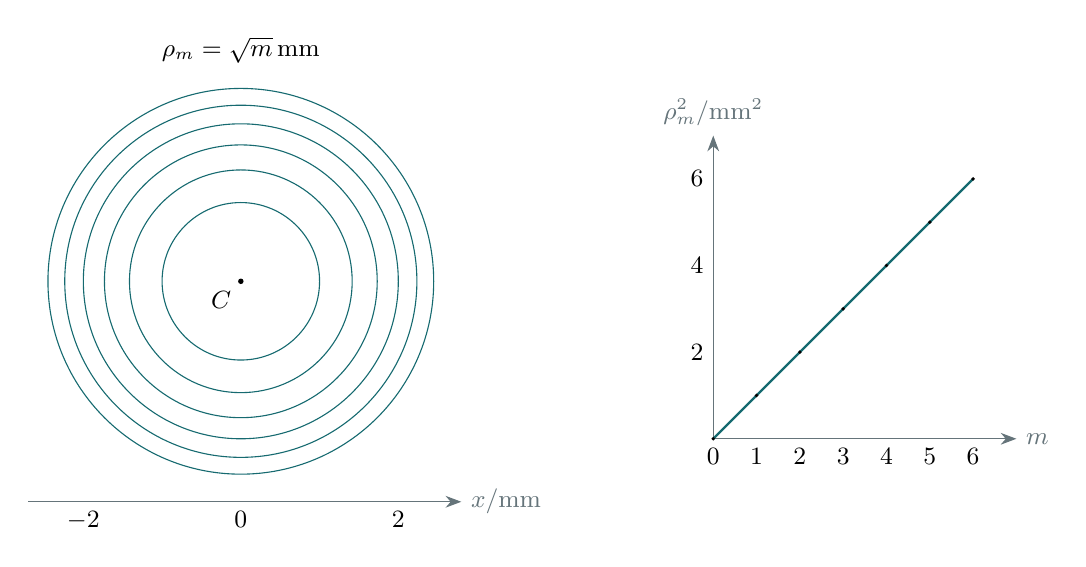
\begin{tikzpicture}[x=1cm,y=1cm]
\begin{scope}[x=1cm,y=1cm]
\draw[color=accent] (0,0)circle(1.000000000000);
\draw[color=accent] (0,0)circle(1.414213562373);
\draw[color=accent] (0,0)circle(1.732050807569);
\draw[color=accent] (0,0)circle(2.000000000000);
\draw[color=accent] (0,0)circle(2.236067977500);
\draw[color=accent] (0,0)circle(2.449489742783);
\fill(0,0)circle(.035);\node[below left]at(0,0){$C$};
\draw[axis](-2.7,-2.8)--(2.8,-2.8)node[right]{$x/\mathrm{mm}$};
\node[below]at(0,-2.8){$0$};\node[below]at(2,-2.8){$2$};\node[below]at(-2,-2.8){$-2$};
\node[above]at(0,2.65){$\rho_m=\sqrt m\,\mathrm{mm}$};\end{scope}
\begin{scope}[shift={(6cm,-2cm)},x=.55cm,y=.55cm]
\draw[axis](0,0)--(7,0)node[right]{$m$};\draw[axis](0,0)--(0,7)node[above]{$\rho_m^2/\mathrm{mm}^2$};
\draw[traj]plot coordinates {(0.000000000000,0.000000000000) (1.000000000000,1.000000000000) (2.000000000000,2.000000000000) (3.000000000000,3.000000000000) (4.000000000000,4.000000000000) (5.000000000000,5.000000000000) (6.000000000000,6.000000000000)};
\fill(0.000000000000,0.000000000000)circle(.045);
\node[below]at(0.000000000000,0.000000000000){$0$};
\fill(1.000000000000,1.000000000000)circle(.045);
\node[below]at(1.000000000000,0.000000000000){$1$};
\fill(2.000000000000,2.000000000000)circle(.045);
\node[below]at(2.000000000000,0.000000000000){$2$};
\fill(3.000000000000,3.000000000000)circle(.045);
\node[below]at(3.000000000000,0.000000000000){$3$};
\fill(4.000000000000,4.000000000000)circle(.045);
\node[below]at(4.000000000000,0.000000000000){$4$};
\fill(5.000000000000,5.000000000000)circle(.045);
\node[below]at(5.000000000000,0.000000000000){$5$};
\fill(6.000000000000,6.000000000000)circle(.045);
\node[below]at(6.000000000000,0.000000000000){$6$};
\node[left]at(0.000000000000,2.000000000000){$2$};
\node[left]at(0.000000000000,4.000000000000){$4$};
\node[left]at(0.000000000000,6.000000000000){$6$};
\end{scope}
\end{tikzpicture}
\figcaption{解图光2.9B\quad 半径随级次平方根增加的圆环}
\end{minipage}\end{center}
如果只要求$\rho/D$很小却需要精确相位，还须检验被丢弃的相位误差$k\rho^4/(8D^3)\ll1$。保留精确几何路程而只近似振幅，可改用$r-D=m\lambda$，得
\[
\rho_m^2=2mD\lambda+m^2\lambda^2.
\]
在振幅中可忽略的小长度差，乘上光学波数后仍可能累积整周相位，所以不能一律令$r=D$。

平面波在同一屏面上具有相同的振幅和相位；球面波在以轴心为圆心的圆周上有相同的振幅和相位。解图光2.9A中，$\rho$确定了斜边$r$，也确定了两波的复振幅、相位差和叠加强度。圆环对称性不依赖近轴展开。屏点坐标为$P(x,y,D)$；$D>0$与$r$均用同一长度单位，振幅比$D/r$无量纲。下文采用同频、同偏振、相干的标量波模型，略去共同的时间因子和相同的强度比例常数。

解图光2.9C用箭头相加表示复振幅合成。记$\delta=k(r-D)$，去掉模为1的共同相位后，精确复振幅是$A[1+(D/r)e^{i\delta}]$。展开模平方，得到两束各自的强度与共轭交叉项：
\[
|\widetilde E_p+\widetilde E_s|^2
=A^2\left(1+\frac{D^2}{r^2}\right)
+A^2\frac Dr(e^{i\delta}+e^{-i\delta}).
\]
在近轴振幅近似下，两矢量等长。解图光2.9C取$\delta=2\pi/3$，合成矢量长度为$A$，对应$I/I_c=1/4$，与$\cos^2(\delta/2)$一致。一般地，
\[
\begin{aligned}
\widetilde E&\simeq Ae^{ikD}\left(1+e^{ik\rho^2/(2D)}\right),\\
I&\simeq A^2(1+e^{i\delta})(1+e^{-i\delta})
=2A^2(1+\cos\delta)=4A^2\cos^2\frac\delta2.
\end{aligned}
\]
这里$\delta\simeq\pi\rho^2/(D\lambda)$。中央$m=0$是一个亮点；第一亮环为$m=1$，$\rho_1=\sqrt{2D\lambda}$，所以$\rho_m=\sqrt m\,\rho_1$。暗环可从$\delta=(2m+1)\pi$得到，$m=0,1,\ldots$。解图光2.9B左侧按$D=1\,\mathrm m$、$\lambda=500\,\mathrm{nm}$画出前六个亮环，右侧将同一批半径平方对级次作图，斜率为$2D\lambda=1\,\mathrm{mm}^2$。相邻亮环还有
\[
\rho_{m+1}^2-\rho_m^2=2D\lambda,\qquad
\Delta\rho_m=\frac{2D\lambda}{\rho_{m+1}+\rho_m}.
\]
外圈分母较大，径向间隔随之减小。这一平方根规律与菲涅耳波带边界的半径规律相同，但这里相邻亮环的路程差增量为$\lambda$；若另以半波带划分，相邻边界的路程差增量则为$\lambda/2$。

解图光2.9D分别画出振幅误差和相位误差，横轴为$q=\rho/D$。采用零阶振幅时，球面波振幅相对$A$的差为
\[
\varepsilon_A=1-\frac1{\sqrt{1+q^2}}\simeq\frac{q^2}{2}.
\]
采用二阶路程时，被忽略的相位大小为
\[
\varepsilon_\phi=2\pi\frac D\lambda
\left(1+\frac{q^2}{2}-\sqrt{1+q^2}\right)
\simeq\frac{\pi D}{4\lambda}q^4.
\]
例如$D/\lambda=10^5$、$q=0.05$，振幅差仅约$0.001248$，相位误差却约$0.4903\,\mathrm{rad}$。所以几何近轴条件$q\ll1$与相位容许误差应分开检验。对第$m$个近轴亮环，$q^2\simeq2m\lambda/D$，相位条件成为$\pi m^2\lambda/D\ll1$。若不满足这一条件，可以保留$r=\sqrt{D^2+\rho^2}$的精确几何，而继续在振幅中取$D/r\simeq1$。

精确几何下，$r-D=m\lambda$给出的是相位相长圆环。若进一步保留真实的$1/r$振幅包络，非中央的径向强度极大位置会略向内移，不能再把它们与这些圆环完全等同。令$t=r-D$、$a=D/(D+t)$，对前面的精确相对强度求导得
\[
\frac{\mathrm d(I/I_c)}{\mathrm dt}
=\frac12\left[a'(a+\cos kt)-ka\sin kt\right],
\qquad a'=-\frac{D}{(D+t)^2}.
\]
当 $t=m\lambda>0$ 时，相位项的导数为零，振幅项仍给出 $a'(a+1)/2<0$。令 $t_m=m\lambda$、$a_m=D/(D+t_m)$，把亮峰写到 $t=t_m+\epsilon$。若 $k(D+t_m)\gg1$，相长点附近 $|\epsilon|\ll\lambda$，可取 $\sin kt\simeq k\epsilon$、$\cos kt\simeq1$。在缓变的振幅因子中用 $a_m$ 和 $a'_m$，由强度导数过零得到
\[
a'_m(a_m+1)-k^2a_m\epsilon\simeq0,\qquad
\epsilon\simeq-\frac{a_m+1}{k^2(D+t_m)}<0.
\]
相位相长圆的半径 $\rho_m=\sqrt{(D+t_m)^2-D^2}$ 随 $t_m$ 增大。对这一关系求导，得到亮峰半径的首项改变量
\[
\delta\rho_m\simeq\frac{D+t_m}{\rho_m}\epsilon
=-\frac{a_m+1}{k^2\rho_m},\qquad m\ge1.
\]
因此保留球面波的振幅衰减后，非中央亮峰稍向轴心移动。前面的亮暗环与间距公式采用近轴和等振幅近似，其误差由 $\varepsilon_\phi$ 与 $\varepsilon_A$ 衡量。

\begin{center}\begin{minipage}{.98\linewidth}\centering
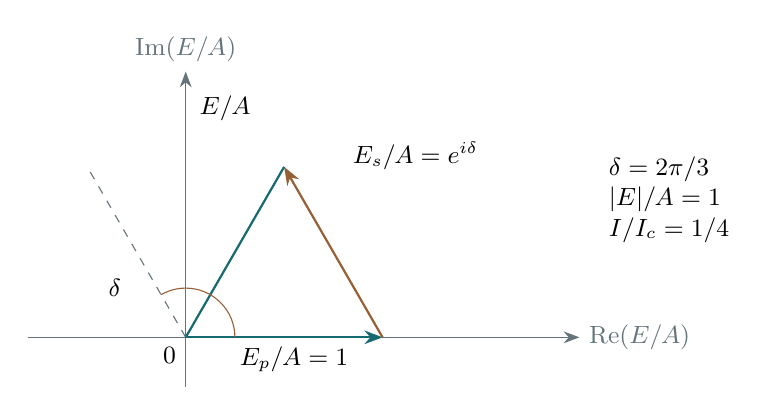
\begin{tikzpicture}[x=2.5cm,y=2.5cm]
\draw[axis](-.8,0)--(2,0)node[right]{$\operatorname{Re}(E/A)$};\draw[axis](0,-.25)--(0,1.35)node[above]{$\operatorname{Im}(E/A)$};\draw[motion](0,0)--(1,0);\draw[force](1,0)--(0.500000000000,0.866025403784);\draw[traj](0,0)--(0.500000000000,0.866025403784);\draw[guide](0,0)--(-0.500000000000,0.866025403784);\draw[thin,color=warm](.25,0)arc[start angle=0,end angle=120,radius=.25];\node[left]at(-.28,.25){$\delta$};\node[below]at(.55,0){$E_p/A=1$};\node[above right]at(.8,.8){$E_s/A=e^{i\delta}$};\node[above]at(.2,1.05){$E/A$};\node[below left]at(0,0){$0$};\node[right,align=left]at(2.1,.7){$\delta=2\pi/3$\\$|E|/A=1$\\$I/I_c=1/4$};
\end{tikzpicture}
\figcaption{解图光2.9C\quad 复平面中两振幅箭头的合成}
\end{minipage}\end{center}

\begin{center}\begin{minipage}{.98\linewidth}\centering
\begin{tikzpicture}[x=1cm,y=1cm]
\begin{scope}[x=43cm,y=.6cm]
\draw[axis](0,0)--(.112,0)node[right]{$q$};\draw[axis](0,0)--(0,5.7)node[above]{$10^3\varepsilon_A$};
\draw[traj]plot coordinates {(0.000000000000,0.000000000000) (0.001000000000,0.000499999625) (0.002000000000,0.001999994000) (0.003000000000,0.004499969625) (0.004000000000,0.007999904001) (0.005000000000,0.012499765630) (0.006000000000,0.017999514014) (0.007000000000,0.024499099662) (0.008000000000,0.031998464082) (0.009000000000,0.040497539791) (0.010000000000,0.049996250312) (0.011000000000,0.060494510179) (0.012000000000,0.071992224933) (0.013000000000,0.084489291133) (0.014000000000,0.097985596353) (0.015000000000,0.112481019184) (0.016000000000,0.127975429242) (0.017000000000,0.144468687166) (0.018000000000,0.161960644626) (0.019000000000,0.180451144322) (0.020000000000,0.199940019993) (0.021000000000,0.220427096416) (0.022000000000,0.241912189416) (0.023000000000,0.264395105865) (0.024000000000,0.287875643689) (0.025000000000,0.312353591877) (0.026000000000,0.337828730479) (0.027000000000,0.364300830617) (0.028000000000,0.391769654487) (0.029000000000,0.420234955371) (0.030000000000,0.449696477633) (0.031000000000,0.480153956737) (0.032000000000,0.511607119244) (0.033000000000,0.544055682824) (0.034000000000,0.577499356264) (0.035000000000,0.611937839468) (0.036000000000,0.647370823474) (0.037000000000,0.683797990455) (0.038000000000,0.721219013730) (0.039000000000,0.759633557771) (0.040000000000,0.799041278211) (0.041000000000,0.839441821852) (0.042000000000,0.880834826679) (0.043000000000,0.923219921860) (0.044000000000,0.966596727764) (0.045000000000,1.010964855962) (0.046000000000,1.056323909246) (0.047000000000,1.102673481632) (0.048000000000,1.150013158370) (0.049000000000,1.198342515960) (0.050000000000,1.247661122155) (0.051000000000,1.297968535979) (0.052000000000,1.349264307733) (0.053000000000,1.401547979007) (0.054000000000,1.454819082691) (0.055000000000,1.509077142991) (0.056000000000,1.564321675434) (0.057000000000,1.620552186885) (0.058000000000,1.677768175555) (0.059000000000,1.735969131018) (0.060000000000,1.795154534221) (0.061000000000,1.855323857497) (0.062000000000,1.916476564577) (0.063000000000,1.978612110606) (0.064000000000,2.041729942153) (0.065000000000,2.105829497229) (0.066000000000,2.170910205295) (0.067000000000,2.236971487282) (0.068000000000,2.304012755601) (0.069000000000,2.372033414159) (0.070000000000,2.441032858373) (0.071000000000,2.511010475188) (0.072000000000,2.581965643086) (0.073000000000,2.653897732107) (0.074000000000,2.726806103860) (0.075000000000,2.800690111544) (0.076000000000,2.875549099956) (0.077000000000,2.951382405515) (0.078000000000,3.028189356275) (0.079000000000,3.105969271937) (0.080000000000,3.184721463875) (0.081000000000,3.264445235144) (0.082000000000,3.345139880502) (0.083000000000,3.426804686425) (0.084000000000,3.509438931126) (0.085000000000,3.593041884571) (0.086000000000,3.677612808496) (0.087000000000,3.763150956430) (0.088000000000,3.849655573707) (0.089000000000,3.937125897486) (0.090000000000,4.025561156771) (0.091000000000,4.114960572431) (0.092000000000,4.205323357213) (0.093000000000,4.296648715768) (0.094000000000,4.388935844665) (0.095000000000,4.482183932414) (0.096000000000,4.576392159484) (0.097000000000,4.671559698321) (0.098000000000,4.767685713371) (0.099000000000,4.864769361100) (0.100000000000,4.962809790011)};
\node[below]at(0.000000000000,0.000000000000){$0$};
\node[below]at(0.050000000000,0.000000000000){$0.05$};
\node[below]at(0.100000000000,0.000000000000){$0.10$};
\node[left]at(0.000000000000,2.500000000000){$2.5$};
\node[left]at(0.000000000000,5.000000000000){$5$};
\end{scope}
\begin{scope}[shift={(7cm,0)},x=43cm,y=.38cm]
\draw[axis](0,0)--(.112,0)node[right]{$q$};\draw[axis](0,0)--(0,9)node[above]{$\varepsilon_\phi/\mathrm{rad}$};
\draw[color=warm,thick]plot coordinates {(0.000000000000,0.000000000000) (0.001000000000,0.000000078540) (0.002000000000,0.000001256635) (0.003000000000,0.000006361696) (0.004000000000,0.000020106032) (0.005000000000,0.000049086772) (0.006000000000,0.000101785770) (0.007000000000,0.000188569479) (0.008000000000,0.000321688794) (0.009000000000,0.000515278866) (0.010000000000,0.000785358896) (0.011000000000,0.001149831887) (0.012000000000,0.001628484383) (0.013000000000,0.002242986166) (0.014000000000,0.003016889937) (0.015000000000,0.003975630956) (0.016000000000,0.005146526669) (0.017000000000,0.006558776292) (0.018000000000,0.008243460374) (0.019000000000,0.010233540335) (0.020000000000,0.012563857968) (0.021000000000,0.015271134922) (0.022000000000,0.018393972144) (0.023000000000,0.021972849310) (0.024000000000,0.026050124210) (0.025000000000,0.030670032121) (0.026000000000,0.035878685140) (0.027000000000,0.041724071497) (0.028000000000,0.048256054832) (0.029000000000,0.055526373454) (0.030000000000,0.063588639565) (0.031000000000,0.072498338457) (0.032000000000,0.082312827682) (0.033000000000,0.093091336197) (0.034000000000,0.104894963475) (0.035000000000,0.117786678595) (0.036000000000,0.131831319297) (0.037000000000,0.147095591017) (0.038000000000,0.163648065891) (0.039000000000,0.181559181727) (0.040000000000,0.200901240955) (0.041000000000,0.221748409552) (0.042000000000,0.244176715928) (0.043000000000,0.268264049797) (0.044000000000,0.294090161014) (0.045000000000,0.321736658386) (0.046000000000,0.351287008455) (0.047000000000,0.382826534255) (0.048000000000,0.416442414041) (0.049000000000,0.452223679988) (0.050000000000,0.490261216872) (0.051000000000,0.530647760709) (0.052000000000,0.573477897381) (0.053000000000,0.618848061230) (0.054000000000,0.666856533620) (0.055000000000,0.717603441477) (0.056000000000,0.771190755804) (0.057000000000,0.827722290166) (0.058000000000,0.887303699147) (0.059000000000,0.950042476782) (0.060000000000,1.016047954965) (0.061000000000,1.085431301823) (0.062000000000,1.158305520073) (0.063000000000,1.234785445345) (0.064000000000,1.314987744479) (0.065000000000,1.399030913804) (0.066000000000,1.487035277377) (0.067000000000,1.579122985207) (0.068000000000,1.675418011448) (0.069000000000,1.776046152569) (0.070000000000,1.881135025488) (0.071000000000,1.990814065698) (0.072000000000,2.105214525347) (0.073000000000,2.224469471309) (0.074000000000,2.348713783216) (0.075000000000,2.478084151473) (0.076000000000,2.612719075243) (0.077000000000,2.752758860409) (0.078000000000,2.898345617509) (0.079000000000,3.049623259642) (0.080000000000,3.206737500358) (0.081000000000,3.369835851511) (0.082000000000,3.539067621096) (0.083000000000,3.714583911057) (0.084000000000,3.896537615068) (0.085000000000,4.085083416293) (0.086000000000,4.280377785118) (0.087000000000,4.482578976861) (0.088000000000,4.691847029452) (0.089000000000,4.908343761094) (0.090000000000,5.132232767898) (0.091000000000,5.363679421489) (0.092000000000,5.602850866592) (0.093000000000,5.849916018594) (0.094000000000,6.105045561078) (0.095000000000,6.368411943336) (0.096000000000,6.640189377856) (0.097000000000,6.920553837786) (0.098000000000,7.209683054371) (0.099000000000,7.507756514373) (0.100000000000,7.814955457457)};
\node[below]at(0.000000000000,0.000000000000){$0$};
\node[below]at(0.050000000000,0.000000000000){$0.05$};
\node[below]at(0.100000000000,0.000000000000){$0.10$};
\node[left]at(0.000000000000,2.000000000000){$2$};
\node[left]at(0.000000000000,4.000000000000){$4$};
\node[left]at(0.000000000000,6.000000000000){$6$};
\node[left]at(0.000000000000,8.000000000000){$8$};
\node[above]at(.05,8.8){$D/\lambda=10^5$};\end{scope}
\end{tikzpicture}
\figcaption{解图光2.9D\quad 同一近轴范围内两种误差的不同量级}
\end{minipage}\end{center}


\Needspace{13\baselineskip}

\pdfbookmark[2]{第 10 题 梅斯林装置中的会聚与发散波}{q10}

\section*{第 10 题\quad 梅斯林装置中的会聚与发散波}\label{q:10}

把同一薄会聚透镜沿直径剖开，两半沿主轴错开$8.0\,\mathrm{cm}$。点光源$S$在轴上，距较近半透镜$L_1$为$60\,\mathrm{cm}$；两半焦距均$f=30\,\mathrm{cm}$。两半分别成像于$S_1',S_2'$，在两像点中间、垂直轴放屏，波长为$500\,\mathrm{nm}$。（1）求近轴干涉条纹的形状。（2）给出相邻环的半径平方差；若中心调为亮纹，求各级亮环半径及间距。保留可能存在的常相位差。



\Needspace{6\baselineskip}

\begin{center}\begin{minipage}{.98\linewidth}\centering
\begin{tikzpicture}[font=\small,x=.05cm,y=.8cm]
\draw[axis](-5,0)--(137,0);\node[right]at(137,0){$z$};
\fill(0,0)circle(1.5pt);\node[below]at(0,0){$S$};
\draw[object](60,0)--(60,1.2);\draw[object](68,0)--(68,-1.2);
\node[above]at(60,1.2){$L_1$};\node[below]at(68,-1.2){$L_2$};
\draw[motion](0,0)--(60,1);\draw[motion](60,1)--(120,0);
\draw[motion](120,0)--(132,-.2);
\draw[motion](0,0)--(68,-1);\draw[motion](68,-1)--(121.6842105263,0);
\fill(120,0)circle(1.2pt);\fill(121.6842105263,0)circle(1.2pt);
\draw[object](120.8421052632,-1.5)--(120.8421052632,1.5);\node[above]at(120.8421052632,1.5){屏};
\draw[guide](120,0)--(109,-.9);\node[below]at(109,-.9){$S_1'$};
\draw[guide](121.6842105263,0)--(133,.65);\node[above]at(133,.65){$S_2'$};
\draw[<->,thin](0,-1.8)--(60,-1.8);\node[below]at(30,-1.8){$60\,\mathrm{cm}$};
\draw[<->,thin](60,1.9)--(68,1.9);\node[above]at(64,1.9){$8\,\mathrm{cm}$};
\node[anchor=north,align=center]at(65,-2.55){轴向从$S$量起：$120$与$121.68421\,\mathrm{cm}$。\\横纵异比例；图示光线不限定半片口径。};
\end{tikzpicture}
\figcaption{图光2.10\quad 两半透镜的像点与夹在其间的屏}
\end{minipage}\end{center}

\Needspace{6\baselineskip}\subsection*{解答}


在图光2.10中从$S$沿轴量坐标，$L_1$位于$60\,\mathrm{cm}$，$L_2$位于$68\,\mathrm{cm}$。薄透镜公式给出
\[
s_1'=60\,\mathrm{cm},\qquad
s_2'=\frac{68\times30}{68-30}=\frac{1020}{19}\,\mathrm{cm}.
\]

这里像距均从各自透镜平面起量。由
\[
\frac1{s_i}+\frac1{s_i'}=\frac1f,\qquad
s_i'=\frac{fs_i}{s_i-f},
\]
将$s_1=60\,\mathrm{cm}$、$s_2=68\,\mathrm{cm}$分别代入，才得到上面的两个像距。像点的共同轴坐标必须再加上各透镜的位置，不能用两个像距之差代替像点间距。
两像点的轴坐标为
\[
z_1'=120\,\mathrm{cm},\qquad
z_2'=\frac{2312}{19}\,\mathrm{cm}=121.68421\,\mathrm{cm}.
\]
屏位于中点，两球心到屏的距离相同，
\[
d_1=d_2=d=\frac{z_2'-z_1'}2=\frac{16}{19}\,\mathrm{cm}
=8.42105\times10^{-3}\,\mathrm m.
\]
\begin{center}\begin{minipage}{.98\linewidth}\centering
\begin{tikzpicture}[font=\small,x=2cm,y=1.15cm]
\draw[axis](-1.4,0)--(1.4,0);\node[right]at(1.4,0){$+z$};
\fill(-1,0)circle(1.4pt);\fill(1,0)circle(1.4pt);
\node[above left]at(-1,0){$S_1'$};\node[above right]at(1,0){$S_2'$};
\draw[object](0,-2)--(0,.45);\node[right,xshift=3pt]at(0,.45){屏};
\draw[motion](-1,0)--(0,-1);\draw[motion](0,-1)--(.65,-1.65);
\draw[force](-.65,-1.65)--(0,-1);\draw[force](0,-1)--(1,0);
\fill(0,-1)circle(1.5pt);\node[right,xshift=9pt]at(0,-1){$P,\ \rho$};
\draw[<->,thin](-1,.85)--(0,.85);\node[above]at(-.5,.85){$d_1$};
\draw[<->,thin](0,.85)--(1,.85);\node[above]at(.5,.85){$d_2$};
\node[anchor=north,align=center]at(0,-2.2){青线：已经过$S_1'$的发散波；暖线：指向$S_2'$的会聚波。\\两束均向右传播；此处横纵异比例。};
\end{tikzpicture}
\figcaption{解图光2.10A\quad 同一点上的两束传播方向与曲率符号}
\end{minipage}\end{center}

取屏面为局部坐标的起算平面，令$\zeta=z-z_{\rm M}$，屏为$\zeta=0$，$O$为轴与屏的交点。解图光2.10A中两个球心的局部坐标分别为$-d_1,+d_2$，而$P$的横向半径为$\rho=\sqrt{x^2+y^2}$。从图A的两个球心分别量到$P$，两段半径均为正长度
\[
R_1=\sqrt{d_1^2+\rho^2},\qquad
R_2=\sqrt{d_2^2+\rho^2}.
\]
采用时间因子$e^{-i\omega t}$。发散球面波的空间因子为$e^{ikR}$，指向未来球心的会聚波为空间因子$e^{-ikR}$。于是本屏面上的两束场可先写成
\[
\widetilde E_1=\frac{B_1}{R_1}e^{ikR_1},\qquad
\widetilde E_2=\frac{B_2}{R_2}e^{-ikR_2},
\]
其中$B_1,B_2$含透镜及传播的恒定复因子。第一束在屏前已经过$S_1'$，第二束到屏时尚未到达$S_2'$；两者都沿$+z$传播，绝不能把会聚波理解成沿$-z$倒行。沿轴的相位梯度在此处分别为$kd_1/R_1$与$kd_2/R_2$，均为正。

在$\rho\ll d_j$下，距离与幅值分别展开为
\[
R_j=d_j+\frac{\rho^2}{2d_j}-\frac{\rho^4}{8d_j^3}
+O\!\left(\frac{\rho^6}{d_j^5}\right),\qquad
\frac1{R_j}=\frac1{d_j}
\left[1-\frac{\rho^2}{2d_j^2}
+O\!\left(\frac{\rho^4}{d_j^4}\right)\right].
\]
幅值的相对变化只有$\rho^2/d_j^2$量级，近轴时可略去；相位增量还乘以$k=2\pi/\lambda$，其中的$\rho^2$项决定图C中的条纹。若只保留二次相位，还应让被舍去的相对相位误差
\[
\frac{k\rho^4}{8}\left(\frac1{d_1^3}+\frac1{d_2^3}\right)\ll1.
\]
解图光2.10B比较正长度$R-d$及其二次式，避免把带符号的球心坐标直接当成距离。将轴上因子分别吸收入$a_je^{i\phi_j}$，便得到下面的近轴复振幅。
\begin{center}\begin{minipage}{.98\linewidth}\centering
\begin{tikzpicture}[font=\small,x=17cm,y=50cm]
\draw[axis](0,0)--(.335,0);\draw[axis](0,0)--(0,.052);
\node[right]at(.335,0){$u=\rho/d$};\node[above]at(0,.052){$(R-d)/d$};
\draw[guide]plot coordinates {(0.0000000000,0.0000000000) (0.0016666667,0.0000013889) (0.0033333333,0.0000055556) (0.0050000000,0.0000125000) (0.0066666667,0.0000222222) (0.0083333333,0.0000347222) (0.0100000000,0.0000500000) (0.0116666667,0.0000680556) (0.0133333333,0.0000888889) (0.0150000000,0.0001125000) (0.0166666667,0.0001388889) (0.0183333333,0.0001680556) (0.0200000000,0.0002000000) (0.0216666667,0.0002347222) (0.0233333333,0.0002722222) (0.0250000000,0.0003125000) (0.0266666667,0.0003555556) (0.0283333333,0.0004013889) (0.0300000000,0.0004500000) (0.0316666667,0.0005013889) (0.0333333333,0.0005555556) (0.0350000000,0.0006125000) (0.0366666667,0.0006722222) (0.0383333333,0.0007347222) (0.0400000000,0.0008000000) (0.0416666667,0.0008680556) (0.0433333333,0.0009388889) (0.0450000000,0.0010125000) (0.0466666667,0.0010888889) (0.0483333333,0.0011680556) (0.0500000000,0.0012500000) (0.0516666667,0.0013347222) (0.0533333333,0.0014222222) (0.0550000000,0.0015125000) (0.0566666667,0.0016055556) (0.0583333333,0.0017013889) (0.0600000000,0.0018000000) (0.0616666667,0.0019013889) (0.0633333333,0.0020055556) (0.0650000000,0.0021125000) (0.0666666667,0.0022222222) (0.0683333333,0.0023347222) (0.0700000000,0.0024500000) (0.0716666667,0.0025680556) (0.0733333333,0.0026888889) (0.0750000000,0.0028125000) (0.0766666667,0.0029388889) (0.0783333333,0.0030680556) (0.0800000000,0.0032000000) (0.0816666667,0.0033347222) (0.0833333333,0.0034722222) (0.0850000000,0.0036125000) (0.0866666667,0.0037555556) (0.0883333333,0.0039013889) (0.0900000000,0.0040500000) (0.0916666667,0.0042013889) (0.0933333333,0.0043555556) (0.0950000000,0.0045125000) (0.0966666667,0.0046722222) (0.0983333333,0.0048347222) (0.1000000000,0.0050000000) (0.1016666667,0.0051680556) (0.1033333333,0.0053388889) (0.1050000000,0.0055125000) (0.1066666667,0.0056888889) (0.1083333333,0.0058680556) (0.1100000000,0.0060500000) (0.1116666667,0.0062347222) (0.1133333333,0.0064222222) (0.1150000000,0.0066125000) (0.1166666667,0.0068055556) (0.1183333333,0.0070013889) (0.1200000000,0.0072000000) (0.1216666667,0.0074013889) (0.1233333333,0.0076055556) (0.1250000000,0.0078125000) (0.1266666667,0.0080222222) (0.1283333333,0.0082347222) (0.1300000000,0.0084500000) (0.1316666667,0.0086680556) (0.1333333333,0.0088888889) (0.1350000000,0.0091125000) (0.1366666667,0.0093388889) (0.1383333333,0.0095680556) (0.1400000000,0.0098000000) (0.1416666667,0.0100347222) (0.1433333333,0.0102722222) (0.1450000000,0.0105125000) (0.1466666667,0.0107555556) (0.1483333333,0.0110013889) (0.1500000000,0.0112500000) (0.1516666667,0.0115013889) (0.1533333333,0.0117555556) (0.1550000000,0.0120125000) (0.1566666667,0.0122722222) (0.1583333333,0.0125347222) (0.1600000000,0.0128000000) (0.1616666667,0.0130680556) (0.1633333333,0.0133388889) (0.1650000000,0.0136125000) (0.1666666667,0.0138888889) (0.1683333333,0.0141680556) (0.1700000000,0.0144500000) (0.1716666667,0.0147347222) (0.1733333333,0.0150222222) (0.1750000000,0.0153125000) (0.1766666667,0.0156055556) (0.1783333333,0.0159013889) (0.1800000000,0.0162000000) (0.1816666667,0.0165013889) (0.1833333333,0.0168055556) (0.1850000000,0.0171125000) (0.1866666667,0.0174222222) (0.1883333333,0.0177347222) (0.1900000000,0.0180500000) (0.1916666667,0.0183680556) (0.1933333333,0.0186888889) (0.1950000000,0.0190125000) (0.1966666667,0.0193388889) (0.1983333333,0.0196680556) (0.2000000000,0.0200000000) (0.2016666667,0.0203347222) (0.2033333333,0.0206722222) (0.2050000000,0.0210125000) (0.2066666667,0.0213555556) (0.2083333333,0.0217013889) (0.2100000000,0.0220500000) (0.2116666667,0.0224013889) (0.2133333333,0.0227555556) (0.2150000000,0.0231125000) (0.2166666667,0.0234722222) (0.2183333333,0.0238347222) (0.2200000000,0.0242000000) (0.2216666667,0.0245680556) (0.2233333333,0.0249388889) (0.2250000000,0.0253125000) (0.2266666667,0.0256888889) (0.2283333333,0.0260680556) (0.2300000000,0.0264500000) (0.2316666667,0.0268347222) (0.2333333333,0.0272222222) (0.2350000000,0.0276125000) (0.2366666667,0.0280055556) (0.2383333333,0.0284013889) (0.2400000000,0.0288000000) (0.2416666667,0.0292013889) (0.2433333333,0.0296055556) (0.2450000000,0.0300125000) (0.2466666667,0.0304222222) (0.2483333333,0.0308347222) (0.2500000000,0.0312500000) (0.2516666667,0.0316680556) (0.2533333333,0.0320888889) (0.2550000000,0.0325125000) (0.2566666667,0.0329388889) (0.2583333333,0.0333680556) (0.2600000000,0.0338000000) (0.2616666667,0.0342347222) (0.2633333333,0.0346722222) (0.2650000000,0.0351125000) (0.2666666667,0.0355555556) (0.2683333333,0.0360013889) (0.2700000000,0.0364500000) (0.2716666667,0.0369013889) (0.2733333333,0.0373555556) (0.2750000000,0.0378125000) (0.2766666667,0.0382722222) (0.2783333333,0.0387347222) (0.2800000000,0.0392000000) (0.2816666667,0.0396680556) (0.2833333333,0.0401388889) (0.2850000000,0.0406125000) (0.2866666667,0.0410888889) (0.2883333333,0.0415680556) (0.2900000000,0.0420500000) (0.2916666667,0.0425347222) (0.2933333333,0.0430222222) (0.2950000000,0.0435125000) (0.2966666667,0.0440055556) (0.2983333333,0.0445013889) (0.3000000000,0.0450000000)};
\draw[traj]plot coordinates {(0.0000000000,0.0000000000) (0.0016666667,0.0000013889) (0.0033333333,0.0000055555) (0.0050000000,0.0000124999) (0.0066666667,0.0000222220) (0.0083333333,0.0000347216) (0.0100000000,0.0000499988) (0.0116666667,0.0000680532) (0.0133333333,0.0000888849) (0.0150000000,0.0001124937) (0.0166666667,0.0001388792) (0.0183333333,0.0001680414) (0.0200000000,0.0001999800) (0.0216666667,0.0002346947) (0.0233333333,0.0002721852) (0.0250000000,0.0003124512) (0.0266666667,0.0003554924) (0.0283333333,0.0004013084) (0.0300000000,0.0004498988) (0.0316666667,0.0005012633) (0.0333333333,0.0005554013) (0.0350000000,0.0006123125) (0.0366666667,0.0006719964) (0.0383333333,0.0007344525) (0.0400000000,0.0007996803) (0.0416666667,0.0008676791) (0.0433333333,0.0009384485) (0.0450000000,0.0010119879) (0.0466666667,0.0010882967) (0.0483333333,0.0011673742) (0.0500000000,0.0012492197) (0.0516666667,0.0013338327) (0.0533333333,0.0014212123) (0.0550000000,0.0015113579) (0.0566666667,0.0016042687) (0.0583333333,0.0016999440) (0.0600000000,0.0017983829) (0.0616666667,0.0018995847) (0.0633333333,0.0020035485) (0.0650000000,0.0021102734) (0.0666666667,0.0022197586) (0.0683333333,0.0023320031) (0.0700000000,0.0024470061) (0.0716666667,0.0025647665) (0.0733333333,0.0026852835) (0.0750000000,0.0028085560) (0.0766666667,0.0029345830) (0.0783333333,0.0030633635) (0.0800000000,0.0031948963) (0.0816666667,0.0033291805) (0.0833333333,0.0034662149) (0.0850000000,0.0036059984) (0.0866666667,0.0037485298) (0.0883333333,0.0038938080) (0.0900000000,0.0040418318) (0.0916666667,0.0041925999) (0.0933333333,0.0043461112) (0.0950000000,0.0045023644) (0.0966666667,0.0046613581) (0.0983333333,0.0048230911) (0.1000000000,0.0049875621) (0.1016666667,0.0051547697) (0.1033333333,0.0053247126) (0.1050000000,0.0054973894) (0.1066666667,0.0056727986) (0.1083333333,0.0058509388) (0.1100000000,0.0060318086) (0.1116666667,0.0062154066) (0.1133333333,0.0064017311) (0.1150000000,0.0065907808) (0.1166666667,0.0067825540) (0.1183333333,0.0069770493) (0.1200000000,0.0071742650) (0.1216666667,0.0073741995) (0.1233333333,0.0075768512) (0.1250000000,0.0077822185) (0.1266666667,0.0079902998) (0.1283333333,0.0082010933) (0.1300000000,0.0084145973) (0.1316666667,0.0086308101) (0.1333333333,0.0088497300) (0.1350000000,0.0090713553) (0.1366666667,0.0092956840) (0.1383333333,0.0095227145) (0.1400000000,0.0097524449) (0.1416666667,0.0099848734) (0.1433333333,0.0102199980) (0.1450000000,0.0104578170) (0.1466666667,0.0106983284) (0.1483333333,0.0109415303) (0.1500000000,0.0111874208) (0.1516666667,0.0114359979) (0.1533333333,0.0116872595) (0.1550000000,0.0119412038) (0.1566666667,0.0121978287) (0.1583333333,0.0124571322) (0.1600000000,0.0127191121) (0.1616666667,0.0129837665) (0.1633333333,0.0132510932) (0.1650000000,0.0135210901) (0.1666666667,0.0137937550) (0.1683333333,0.0140690860) (0.1700000000,0.0143470806) (0.1716666667,0.0146277369) (0.1733333333,0.0149110525) (0.1750000000,0.0151970252) (0.1766666667,0.0154856528) (0.1783333333,0.0157769331) (0.1800000000,0.0160708637) (0.1816666667,0.0163674423) (0.1833333333,0.0166666667) (0.1850000000,0.0169685344) (0.1866666667,0.0172730432) (0.1883333333,0.0175801907) (0.1900000000,0.0178899744) (0.1916666667,0.0182023920) (0.1933333333,0.0185174411) (0.1950000000,0.0188351191) (0.1966666667,0.0191554238) (0.1983333333,0.0194783524) (0.2000000000,0.0198039027) (0.2016666667,0.0201320721) (0.2033333333,0.0204628579) (0.2050000000,0.0207962578) (0.2066666667,0.0211322692) (0.2083333333,0.0214708893) (0.2100000000,0.0218121158) (0.2116666667,0.0221559459) (0.2133333333,0.0225023771) (0.2150000000,0.0228514066) (0.2166666667,0.0232030319) (0.2183333333,0.0235572502) (0.2200000000,0.0239140589) (0.2216666667,0.0242734552) (0.2233333333,0.0246354365) (0.2250000000,0.0250000000) (0.2266666667,0.0253671429) (0.2283333333,0.0257368625) (0.2300000000,0.0261091560) (0.2316666667,0.0264840205) (0.2333333333,0.0268614534) (0.2350000000,0.0272414517) (0.2366666667,0.0276240125) (0.2383333333,0.0280091331) (0.2400000000,0.0283968106) (0.2416666667,0.0287870420) (0.2433333333,0.0291798245) (0.2450000000,0.0295751551) (0.2466666667,0.0299730309) (0.2483333333,0.0303734490) (0.2500000000,0.0307764064) (0.2516666667,0.0311819001) (0.2533333333,0.0315899271) (0.2550000000,0.0320004845) (0.2566666667,0.0324135692) (0.2583333333,0.0328291781) (0.2600000000,0.0332473082) (0.2616666667,0.0336679566) (0.2633333333,0.0340911200) (0.2650000000,0.0345167954) (0.2666666667,0.0349449798) (0.2683333333,0.0353756699) (0.2700000000,0.0358088627) (0.2716666667,0.0362445550) (0.2733333333,0.0366827437) (0.2750000000,0.0371234256) (0.2766666667,0.0375665976) (0.2783333333,0.0380122564) (0.2800000000,0.0384603989) (0.2816666667,0.0389110217) (0.2833333333,0.0393641218) (0.2850000000,0.0398196959) (0.2866666667,0.0402777407) (0.2883333333,0.0407382529) (0.2900000000,0.0412012294) (0.2916666667,0.0416666667) (0.2933333333,0.0421345616) (0.2950000000,0.0426049108) (0.2966666667,0.0430777110) (0.2983333333,0.0435529588) (0.3000000000,0.0440306509)};
\node[below left]at(0,0){$0$};\node[left]at(0,.02){$.02$};\node[left]at(0,.04){$.04$};
\node[below]at(.1,0){$.1$};\node[below]at(.2,0){$.2$};\node[below]at(.3,0){$.3$};
\node[anchor=north,align=center]at(.16,-.011){实线：$\sqrt{1+u^2}-1$；虚线：$u^2/2$。\\振幅可取常量时，相位仍须保留二次项。};
\end{tikzpicture}
\figcaption{解图光2.10B\quad 球面距离的二次近似与相位增量}
\end{minipage}\end{center}

解图光2.10A中，来自$S_1'$的波已经发散，指向$S_2'$的波仍会聚。取屏上半径$\rho$，两者的近轴复振幅写成
\[
\widetilde E_1=a_1e^{i\phi_1}\exp\frac{ik\rho^2}{2d_1},\qquad
\widetilde E_2=a_2e^{i\phi_2}\exp\left(-\frac{ik\rho^2}{2d_2}\right).
\]
屏在两球心之间，图中已过焦点的波前向外展开，另一波前仍向球心会聚。因此两束曲率异号，相减时得到曲率大小之和：
\[
\delta(\rho)=\delta_0+\frac{k\rho^2}{2}\left(\frac1{d_1}+\frac1{d_2}\right),\qquad
\delta_0=\phi_1-\phi_2.
\]

用图A中从$P$量到两球心的正距离，先写相位差
\[
\delta_{\rm sph}(\rho)
=\delta_0+k\big[(R_1-d_1)+(R_2-d_2)\big].
\]
因此两项曲率大小相加。用上面的二次展开，正好恢复$\delta(\rho)$；若只因屏到两像距离相等就写$R_1-R_2=0$，便把会聚束的相位符号丢掉了。两场相加后取模平方，
\[
|\widetilde E_1+\widetilde E_2|^2
=a_1^2+a_2^2+2a_1a_2\cos(\phi_1-\phi_2+
\tfrac{k\rho^2}{2d_1}+\tfrac{k\rho^2}{2d_2}),
\]
这给出强度中的交叉项。
强度为$I_1+I_2+2\sqrt{I_1I_2}\cos\delta$。在共同照明区内等相位线是同心圆，但有限半片孔径可能只照出圆的一部分。

相邻亮环无论$\delta_0$为何值，都满足
\[
\boxed{\Delta(\rho^2)=\frac{2\lambda}{1/d_1+1/d_2}=\lambda d
=4.210526\times10^{-9}\,\mathrm{m^2}}.
\]

这里的亮、暗级次是近轴且幅值缓变时的相位条件。令
\[
C=\frac1{d_1}+\frac1{d_2},\qquad
\eta=\frac{\delta_0}{2\pi},\qquad H=\frac{2\lambda}{C},
\]
则相长与相消分别给
\[
\rho_{\rm M,m}^2=H(m-\eta),\qquad
\rho_{\rm m,m}^2=H(m+\tfrac12-\eta),
\]
分别取使右端非负且位于共同照明区内的整数$m$。改变$\delta_0$平移的是$\rho^2$级次，不能仅从$d_1=d_2$断言中心亮。若幅值随半径的变化不可忽略，完整强度的严格驻点还会受包络导数影响，需另行求导。
\begin{center}\begin{minipage}{.98\linewidth}\centering
\begin{tikzpicture}[font=\small,x=1.25cm,y=1.3cm]
\draw[axis](0,0)--(4.4,0);\draw[axis](0,0)--(0,2.35);
\node[right]at(4.4,0){$q=\rho^2/(\lambda d)$};\node[above]at(0,2.35){$I/(I_1+I_2)$};
\draw[traj]plot coordinates {(0.0000000000,2.0000000000) (0.0125000000,1.9969173337) (0.0250000000,1.9876883406) (0.0375000000,1.9723699204) (0.0500000000,1.9510565163) (0.0625000000,1.9238795325) (0.0750000000,1.8910065242) (0.0875000000,1.8526401644) (0.1000000000,1.8090169944) (0.1125000000,1.7604059656) (0.1250000000,1.7071067812) (0.1375000000,1.6494480483) (0.1500000000,1.5877852523) (0.1625000000,1.5224985647) (0.1750000000,1.4539904997) (0.1875000000,1.3826834324) (0.2000000000,1.3090169944) (0.2125000000,1.2334453639) (0.2250000000,1.1564344650) (0.2375000000,1.0784590957) (0.2500000000,1.0000000000) (0.2625000000,0.9215409043) (0.2750000000,0.8435655350) (0.2875000000,0.7665546361) (0.3000000000,0.6909830056) (0.3125000000,0.6173165676) (0.3250000000,0.5460095003) (0.3375000000,0.4775014353) (0.3500000000,0.4122147477) (0.3625000000,0.3505519517) (0.3750000000,0.2928932188) (0.3875000000,0.2395940344) (0.4000000000,0.1909830056) (0.4125000000,0.1473598356) (0.4250000000,0.1089934758) (0.4375000000,0.0761204675) (0.4500000000,0.0489434837) (0.4625000000,0.0276300796) (0.4750000000,0.0123116594) (0.4875000000,0.0030826663) (0.5000000000,0.0000000000) (0.5125000000,0.0030826663) (0.5250000000,0.0123116594) (0.5375000000,0.0276300796) (0.5500000000,0.0489434837) (0.5625000000,0.0761204675) (0.5750000000,0.1089934758) (0.5875000000,0.1473598356) (0.6000000000,0.1909830056) (0.6125000000,0.2395940344) (0.6250000000,0.2928932188) (0.6375000000,0.3505519517) (0.6500000000,0.4122147477) (0.6625000000,0.4775014353) (0.6750000000,0.5460095003) (0.6875000000,0.6173165676) (0.7000000000,0.6909830056) (0.7125000000,0.7665546361) (0.7250000000,0.8435655350) (0.7375000000,0.9215409043) (0.7500000000,1.0000000000) (0.7625000000,1.0784590957) (0.7750000000,1.1564344650) (0.7875000000,1.2334453639) (0.8000000000,1.3090169944) (0.8125000000,1.3826834324) (0.8250000000,1.4539904997) (0.8375000000,1.5224985647) (0.8500000000,1.5877852523) (0.8625000000,1.6494480483) (0.8750000000,1.7071067812) (0.8875000000,1.7604059656) (0.9000000000,1.8090169944) (0.9125000000,1.8526401644) (0.9250000000,1.8910065242) (0.9375000000,1.9238795325) (0.9500000000,1.9510565163) (0.9625000000,1.9723699204) (0.9750000000,1.9876883406) (0.9875000000,1.9969173337) (1.0000000000,2.0000000000) (1.0125000000,1.9969173337) (1.0250000000,1.9876883406) (1.0375000000,1.9723699204) (1.0500000000,1.9510565163) (1.0625000000,1.9238795325) (1.0750000000,1.8910065242) (1.0875000000,1.8526401644) (1.1000000000,1.8090169944) (1.1125000000,1.7604059656) (1.1250000000,1.7071067812) (1.1375000000,1.6494480483) (1.1500000000,1.5877852523) (1.1625000000,1.5224985647) (1.1750000000,1.4539904997) (1.1875000000,1.3826834324) (1.2000000000,1.3090169944) (1.2125000000,1.2334453639) (1.2250000000,1.1564344650) (1.2375000000,1.0784590957) (1.2500000000,1.0000000000) (1.2625000000,0.9215409043) (1.2750000000,0.8435655350) (1.2875000000,0.7665546361) (1.3000000000,0.6909830056) (1.3125000000,0.6173165676) (1.3250000000,0.5460095003) (1.3375000000,0.4775014353) (1.3500000000,0.4122147477) (1.3625000000,0.3505519517) (1.3750000000,0.2928932188) (1.3875000000,0.2395940344) (1.4000000000,0.1909830056) (1.4125000000,0.1473598356) (1.4250000000,0.1089934758) (1.4375000000,0.0761204675) (1.4500000000,0.0489434837) (1.4625000000,0.0276300796) (1.4750000000,0.0123116594) (1.4875000000,0.0030826663) (1.5000000000,0.0000000000) (1.5125000000,0.0030826663) (1.5250000000,0.0123116594) (1.5375000000,0.0276300796) (1.5500000000,0.0489434837) (1.5625000000,0.0761204675) (1.5750000000,0.1089934758) (1.5875000000,0.1473598356) (1.6000000000,0.1909830056) (1.6125000000,0.2395940344) (1.6250000000,0.2928932188) (1.6375000000,0.3505519517) (1.6500000000,0.4122147477) (1.6625000000,0.4775014353) (1.6750000000,0.5460095003) (1.6875000000,0.6173165676) (1.7000000000,0.6909830056) (1.7125000000,0.7665546361) (1.7250000000,0.8435655350) (1.7375000000,0.9215409043) (1.7500000000,1.0000000000) (1.7625000000,1.0784590957) (1.7750000000,1.1564344650) (1.7875000000,1.2334453639) (1.8000000000,1.3090169944) (1.8125000000,1.3826834324) (1.8250000000,1.4539904997) (1.8375000000,1.5224985647) (1.8500000000,1.5877852523) (1.8625000000,1.6494480483) (1.8750000000,1.7071067812) (1.8875000000,1.7604059656) (1.9000000000,1.8090169944) (1.9125000000,1.8526401644) (1.9250000000,1.8910065242) (1.9375000000,1.9238795325) (1.9500000000,1.9510565163) (1.9625000000,1.9723699204) (1.9750000000,1.9876883406) (1.9875000000,1.9969173337) (2.0000000000,2.0000000000) (2.0125000000,1.9969173337) (2.0250000000,1.9876883406) (2.0375000000,1.9723699204) (2.0500000000,1.9510565163) (2.0625000000,1.9238795325) (2.0750000000,1.8910065242) (2.0875000000,1.8526401644) (2.1000000000,1.8090169944) (2.1125000000,1.7604059656) (2.1250000000,1.7071067812) (2.1375000000,1.6494480483) (2.1500000000,1.5877852523) (2.1625000000,1.5224985647) (2.1750000000,1.4539904997) (2.1875000000,1.3826834324) (2.2000000000,1.3090169944) (2.2125000000,1.2334453639) (2.2250000000,1.1564344650) (2.2375000000,1.0784590957) (2.2500000000,1.0000000000) (2.2625000000,0.9215409043) (2.2750000000,0.8435655350) (2.2875000000,0.7665546361) (2.3000000000,0.6909830056) (2.3125000000,0.6173165676) (2.3250000000,0.5460095003) (2.3375000000,0.4775014353) (2.3500000000,0.4122147477) (2.3625000000,0.3505519517) (2.3750000000,0.2928932188) (2.3875000000,0.2395940344) (2.4000000000,0.1909830056) (2.4125000000,0.1473598356) (2.4250000000,0.1089934758) (2.4375000000,0.0761204675) (2.4500000000,0.0489434837) (2.4625000000,0.0276300796) (2.4750000000,0.0123116594) (2.4875000000,0.0030826663) (2.5000000000,0.0000000000) (2.5125000000,0.0030826663) (2.5250000000,0.0123116594) (2.5375000000,0.0276300796) (2.5500000000,0.0489434837) (2.5625000000,0.0761204675) (2.5750000000,0.1089934758) (2.5875000000,0.1473598356) (2.6000000000,0.1909830056) (2.6125000000,0.2395940344) (2.6250000000,0.2928932188) (2.6375000000,0.3505519517) (2.6500000000,0.4122147477) (2.6625000000,0.4775014353) (2.6750000000,0.5460095003) (2.6875000000,0.6173165676) (2.7000000000,0.6909830056) (2.7125000000,0.7665546361) (2.7250000000,0.8435655350) (2.7375000000,0.9215409043) (2.7500000000,1.0000000000) (2.7625000000,1.0784590957) (2.7750000000,1.1564344650) (2.7875000000,1.2334453639) (2.8000000000,1.3090169944) (2.8125000000,1.3826834324) (2.8250000000,1.4539904997) (2.8375000000,1.5224985647) (2.8500000000,1.5877852523) (2.8625000000,1.6494480483) (2.8750000000,1.7071067812) (2.8875000000,1.7604059656) (2.9000000000,1.8090169944) (2.9125000000,1.8526401644) (2.9250000000,1.8910065242) (2.9375000000,1.9238795325) (2.9500000000,1.9510565163) (2.9625000000,1.9723699204) (2.9750000000,1.9876883406) (2.9875000000,1.9969173337) (3.0000000000,2.0000000000) (3.0125000000,1.9969173337) (3.0250000000,1.9876883406) (3.0375000000,1.9723699204) (3.0500000000,1.9510565163) (3.0625000000,1.9238795325) (3.0750000000,1.8910065242) (3.0875000000,1.8526401644) (3.1000000000,1.8090169944) (3.1125000000,1.7604059656) (3.1250000000,1.7071067812) (3.1375000000,1.6494480483) (3.1500000000,1.5877852523) (3.1625000000,1.5224985647) (3.1750000000,1.4539904997) (3.1875000000,1.3826834324) (3.2000000000,1.3090169944) (3.2125000000,1.2334453639) (3.2250000000,1.1564344650) (3.2375000000,1.0784590957) (3.2500000000,1.0000000000) (3.2625000000,0.9215409043) (3.2750000000,0.8435655350) (3.2875000000,0.7665546361) (3.3000000000,0.6909830056) (3.3125000000,0.6173165676) (3.3250000000,0.5460095003) (3.3375000000,0.4775014353) (3.3500000000,0.4122147477) (3.3625000000,0.3505519517) (3.3750000000,0.2928932188) (3.3875000000,0.2395940344) (3.4000000000,0.1909830056) (3.4125000000,0.1473598356) (3.4250000000,0.1089934758) (3.4375000000,0.0761204675) (3.4500000000,0.0489434837) (3.4625000000,0.0276300796) (3.4750000000,0.0123116594) (3.4875000000,0.0030826663) (3.5000000000,0.0000000000) (3.5125000000,0.0030826663) (3.5250000000,0.0123116594) (3.5375000000,0.0276300796) (3.5500000000,0.0489434837) (3.5625000000,0.0761204675) (3.5750000000,0.1089934758) (3.5875000000,0.1473598356) (3.6000000000,0.1909830056) (3.6125000000,0.2395940344) (3.6250000000,0.2928932188) (3.6375000000,0.3505519517) (3.6500000000,0.4122147477) (3.6625000000,0.4775014353) (3.6750000000,0.5460095003) (3.6875000000,0.6173165676) (3.7000000000,0.6909830056) (3.7125000000,0.7665546361) (3.7250000000,0.8435655350) (3.7375000000,0.9215409043) (3.7500000000,1.0000000000) (3.7625000000,1.0784590957) (3.7750000000,1.1564344650) (3.7875000000,1.2334453639) (3.8000000000,1.3090169944) (3.8125000000,1.3826834324) (3.8250000000,1.4539904997) (3.8375000000,1.5224985647) (3.8500000000,1.5877852523) (3.8625000000,1.6494480483) (3.8750000000,1.7071067812) (3.8875000000,1.7604059656) (3.9000000000,1.8090169944) (3.9125000000,1.8526401644) (3.9250000000,1.8910065242) (3.9375000000,1.9238795325) (3.9500000000,1.9510565163) (3.9625000000,1.9723699204) (3.9750000000,1.9876883406) (3.9875000000,1.9969173337) (4.0000000000,2.0000000000)};
\node[left]at(0,2){$2$};\node[below left]at(0,0){$0$};
\node[below]at(1,0){$1$};\fill(1,2)circle(1.2pt);
\node[below]at(2,0){$2$};\fill(2,2)circle(1.2pt);
\node[below]at(3,0){$3$};\fill(3,2)circle(1.2pt);
\node[below]at(4,0){$4$};\fill(4,2)circle(1.2pt);
\node[anchor=north]at(2,-.5){取$I_1=I_2,\ \delta_0=0$；亮环在$q=m$，而$\rho_m=\sqrt m\,\rho_1$。};
\end{tikzpicture}
\figcaption{解图光2.10C\quad 平方半径等间隔，实际半径不等间隔}
\end{minipage}\end{center}

若通过光程补偿使中心亮，即$\delta_0=0\pmod{2\pi}$，则
\[
\rho_m=\sqrt{m\lambda d}
=6.48886\times10^{-5}\sqrt m\,\mathrm m,\quad m=0,1,\ldots,
\]
\[
\Delta\rho_m=6.48886\times10^{-5}(\sqrt{m+1}-\sqrt m)\,\mathrm m.
\]
环间距向外减小。一般$\delta_0$应保留在$\rho_m^2=[2m\lambda-\lambda\delta_0/\pi]/(1/d_1+1/d_2)$中，取使半径平方非负的整数$m$；不能仅由曲率断言中心必亮。半片的常光程及经过焦区的相位影响属于$\delta_0$。

解图光2.10C以$q=\rho^2/(\lambda d)$作横轴，相邻峰在$q$中相隔1。换回真实半径后，
\[
\rho_{m+1}-\rho_m
=\frac{\lambda d}{\rho_{m+1}+\rho_m},
\]
相邻环的半径和随$m$增大，因此外侧间距变小。第一、第二个亮环半径分别约为$64.8886\,\mu\mathrm m$、$91.7663\,\mu\mathrm m$；两环相距约$26.8777\,\mu\mathrm m$。这些数值沿用精确$d=16/19\,\mathrm{cm}$，没有在小差值形成前先把像距舍入。

再按两半片的瞳面检查图D中的照明边界。设两个半片的半径分别为$a_1,a_2$，上半片$L_1$的瞳面坐标为$\boldsymbol u_1$，下半片$L_2$为$\boldsymbol u_2$。屏上横向坐标由直线成像关系给出
\[
\boldsymbol r_{\perp,1}=-\frac{d_1}{s_1'}\boldsymbol u_1,\qquad
\boldsymbol r_{\perp,2}=+\frac{d_2}{s_2'}\boldsymbol u_2 .
\]
第一式已越过像点，符号反转；第二式还在像点之前，符号保持。因$u_{1y}>0,u_{2y}<0$，两束都落在屏的$y<0$侧，理想半圆瞳面给出的共同照明半径为
\[
\rho_c=\min\left(\frac{a_1d_1}{s_1'},\frac{a_2d_2}{s_2'}\right).
\]
解图光2.10D仅选$a_1=a_2=10\,\mathrm{mm}$示出口径效果：$\rho_c=0.14035\,\mathrm{mm}$，可照到四条正级次亮环弧。圆的方程适用于相位分布；被遮去的上半圆并不会因同相而自行发亮。题设的“中心调亮”规定轴上外推的相位，$O$又处在理想切边的几何边界，紧贴边缘的真实强度还须用衍射描述。
\begin{center}\begin{minipage}{.98\linewidth}\centering
\begin{tikzpicture}[font=\small,x=17cm,y=17cm]
\fill[teal!7](-0.1403508772,0)arc(180:360:0.1403508772)--cycle;
\draw[axis](-.18,0)--(.19,0);\draw[axis](0,-.18)--(0,.055);
\node[right]at(.19,0){$x/\mathrm{mm}$};\node[above]at(0,.055){$y/\mathrm{mm}$};\node[above left]at(0,0){$O$};
\draw[traj](-0.0648885685,0)arc(180:360:0.0648885685);
\draw[traj](-0.0917662935,0)arc(180:360:0.0917662935);
\draw[traj](-0.1123902974,0)arc(180:360:0.1123902974);
\draw[traj](-0.1297771369,0)arc(180:360:0.1297771369);\draw[object](-0.1403508772,0)arc(180:360:0.1403508772);\draw[guide](-0.1568627451,0)arc(180:360:0.1568627451);
\node[above]at(.1,0){$.10$};\draw[guide](-.18,-.1)--(0,-.1);\node[left]at(-.18,-.1){$-.10$};
\node[above right]at(.13,.025){$\rho_c$};
\node[anchor=north,align=center]at(0,-.205){选$a_1=a_2=10\,\mathrm{mm}$作口径示例；\\共同照明只在下半圆内，图中有四条亮环弧。};
\end{tikzpicture}
\figcaption{解图光2.10D\quad 同心圆的相位轨迹与半片共同照明区}
\end{minipage}\end{center}


\Needspace{13\baselineskip}

\pdfbookmark[2]{第 11 题 有限洛埃镜的条纹与谱宽}{q11}

\section*{第 11 题\quad 有限洛埃镜的条纹与谱宽}\label{q:11}

水平洛埃镜长度$B=5.00\,\mathrm{cm}$，镜左端$x=0$、右端$x=B$，屏在$x=B+C$，其中$C=5.00\,\mathrm m$。点光源在$(-A,d)$，$A=2.00\,\mathrm{cm}$、$d=0.500\,\mathrm{mm}$，波长$\lambda=600\,\mathrm{nm}$，反射附加相位为$\pi$。（1）求近轴条纹间距。（2）求共同照明高度范围和实际亮纹数。（3）为在全部共同区内保持可辨条纹，对光谱宽度有何要求？给出所采用的可见度判据。

\begin{center}\begin{minipage}{.98\linewidth}\centering
\begin{tikzpicture}
\begin{scope}[x=.52cm,y=.85cm]
\draw[axis] (-2.8,0)--(9.2,0) node[right] {$x/\mathrm{cm}$};
\draw[axis] (0,-.75)--(0,2.45) node[above] {$y/\mathrm{mm}$};
\draw[very thick] (0,0)--(5,0);
\fill (-2,.5) circle(1.3pt) node[above left] {$S$};
\fill (-2,-.5) circle(1.3pt) node[below left] {$S'$};
\draw[motion] (-2,.5)--(0,0);
\draw[motion] (0,0)--(8,2) node[above right] {至$H_2$};
\draw[force] (-2,.5)--(5,0);
\draw[force] (5,0)--(8,.214286);
\node[above] at (7.8,.45) {至$H_1$};
\draw[guide] (-2,-.5)--(0,0);
\draw[guide] (-2,-.5)--(5,0);
\draw[muted] (5,0)--(5,-.08) node[below] {$5$};
\node[left] at (0,1.2) {$x=0$};
\draw[muted] (-2,0)--(-2,-.08) node[below left] {$-2$};
\end{scope}
\begin{scope}[shift={(7.5cm,0)},x=1cm,y=.025cm]
\draw[axis] (0,0)--(0,145) node[above] {$y/\mathrm{mm}$};
\fill[accent,opacity=.12] (-.12,35.714286) rectangle (.12,126.25);
\draw[object] (0,35.714286)--(0,126.25);
\draw[accent,fill=white] (0,35.714286) circle(1.4pt);
\draw[accent,fill=white] (0,126.25) circle(1.4pt);
\draw[muted] (-.12,35.714286)--(.12,35.714286);
\draw[muted] (-.12,126.25)--(.12,126.25);
\node[right,align=left] at (.18,35.714286) {$H_1$\\$35.7143$};
\node[right,align=left] at (.18,126.25) {$H_2$\\$126.250$};
\node[below,align=center] at (.5,-8) {屏截线\\$x=5.05\,\mathrm m$};
\end{scope}
\end{tikzpicture}
\figcaption{图光2.11\quad 左：镜旁局部；右：屏上共同照明区}
\end{minipage}\end{center}

镜面两端作为共同区边界，不纳入计数；忽略衍射与遮挡，两路取共同的垂直纸面线偏振，光源和虚像保持相干。讨论谱宽时先采用等幅两束、反射相位在窄带内恒为$\pi$的理想模型，再说明谱形和阈值。图左的坐标单位为厘米和毫米，两条边缘出射线继续传播到右图屏上的$H_2,H_1$。

\Needspace{6\baselineskip}\subsection*{解答}


在图光2.11的左侧局部图中，镜面为$y=0$、$0\le x\le B$；$S=(-A,d)$，$S'=(-A,-d)$。取屏点$P=(B+C,y)$。右图阴影段从$H_1$延伸到$H_2$，其中每个屏点都能接到直射光与镜上反射光。用虚像法把反射折线路程$SM+MP$化为直线$S'P$，但实际光线仍是上半空间的$SMP$。

解图光2.11A中光源$S$与虚像$S'$的间距为$2d$，二者到屏的水平距离均为$D=A+B+C=5.07\,\mathrm m$。屏上点$P$高度为$y$，两路几何差为
\[
\Delta(y)=\sqrt{D^2+(y+d)^2}-\sqrt{D^2+(y-d)^2}
\simeq\frac{2dy}{D}.
\]
所以近轴间距为$p=\lambda D/(2d)=3.042\,\mathrm{mm}$。有反射相位$\pi$，亮纹条件为$\Delta=(m+\tfrac12)\lambda$。
\begin{center}\begin{minipage}{.98\linewidth}\centering
\begin{tikzpicture}[x=.62cm,y=1.1cm]
\draw[axis] (-2.8,0)--(8.8,0) node[right] {$x/\mathrm{cm}$};
\draw[axis] (0,-.8)--(0,2.45) node[above] {$y/\mathrm{mm}$};
\draw[very thick] (0,0)--(5,0);
\draw[thin,muted] (-2,.5)--(0,0)--(8,2) node[above right] {至$H_2$};
\draw[thin,muted] (-2,.5)--(5,0)--(8,.214286) node[above right] {至$H_1$};
\draw[guide] (-2,-.5)--(0,0);
\draw[guide] (-2,-.5)--(5,0);
\fill (-2,.5) circle(1.3pt) node[above left] {$S$};
\fill (-2,-.5) circle(1.3pt) node[below left] {$S'$};
\fill (2,0) circle(1.3pt) node[below right,yshift=-9pt] {$M$};
\draw[motion] (-2,.5)--(2,0);
\draw[motion] (2,0)--(8,.75) node[above right] {反射后至$P$};
\draw[guide] (-2,-.5)--(2,0);
\draw[force] (-2,.5)--(8,1.730276);
\node[above left] at (8,1.730276) {直射至$P$};
\draw[muted] (2,0)--(2,-.08) node[below left,yshift=-9pt] {$2$};
\draw[muted] (5,0)--(5,-.08) node[below] {$5$};
\node[below,align=center] at (3,-.9) {$x_r=2.00\,\mathrm{cm}$，$P=(5.05\,\mathrm m,62.875\,\mathrm{mm})$\\局部截断，两条实线继续传播至同一$P$};
\end{tikzpicture}
\figcaption{解图光2.11A\quad 虚像连线确定真实反射点}
\end{minipage}\end{center}

解图光2.11A给出一个可核算的中间光线：取$x_r=2.00\,\mathrm{cm}$，由$S'MP$共线得到$y=62.875\,\mathrm{mm}$。灰色边缘光线给出$H_1,H_2$，绿色折线才是此$P$的实际反射路径，棕线为直射路径。图只画到镜旁$x=8\,\mathrm{cm}$；两束随后到达同一个$P$，没有在局部截断处相交。

反射点必须落在镜段$0<x<B$上。$S'P$与$y=0$交于
\[
x_r=-A+\frac{dD}{y+d}.
\]
由$0<x_r<B$解得共同区
\[
H_1=\frac{Cd}{A+B}=35.7143\,\mathrm{mm}<y<
H_2=\frac{(B+C)d}{A}=126.250\,\mathrm{mm}.
\]
从$x_r=-A+dD/(y+d)$可见，$y$增加时反射点向镜左端移动；在右端$x_r=B$取得较低边界$H_1$，在左端$x_r=0$取得较高边界$H_2$。这里使用的直线截距关系是精确几何，不需要小角近似。
\begin{center}\begin{minipage}{.98\linewidth}\centering
\begin{tikzpicture}[x=1.2cm,y=0.022cm]
\draw[axis] (0.000000,0)--(5.200000,0) node[right] {$x_r/\mathrm{cm}$};
\draw[axis] (0.000000,0)--(0.000000,153.400000) node[above] {$y/\mathrm{mm}$};
\draw[traj] plot coordinates {(0,126.25) (0.052083,123.032995) (0.104167,119.975248) (0.15625,117.065217) (0.208333,114.292453) (0.260417,111.647465) (0.3125,109.121622) (0.364583,106.707048) (0.416667,104.396552) (0.46875,102.183544) (0.520833,100.061983) (0.572917,98.026316) (0.625,96.071429) (0.677083,94.192607) (0.729167,92.385496) (0.78125,90.646067) (0.833333,88.970588) (0.885417,87.355596) (0.9375,85.797872) (0.989583,84.294425) (1.041667,82.842466) (1.09375,81.439394) (1.145833,80.082781) (1.197917,78.770358) (1.25,77.5) (1.302083,76.269716) (1.354167,75.07764) (1.40625,73.922018) (1.458333,72.801205) (1.510417,71.71365) (1.5625,70.657895) (1.614583,69.632565) (1.666667,68.636364) (1.71875,67.668067) (1.770833,66.726519) (1.822917,65.810627) (1.875,64.919355) (1.927083,64.051724) (1.979167,63.206806) (2.03125,62.383721) (2.083333,61.581633) (2.135417,60.799748) (2.1875,60.037313) (2.239583,59.293612) (2.291667,58.567961) (2.34375,57.859712) (2.395833,57.168246) (2.447917,56.492974) (2.5,55.833333) (2.552083,55.188787) (2.604167,54.558824) (2.65625,53.942953) (2.708333,53.340708) (2.760417,52.751641) (2.8125,52.175325) (2.864583,51.611349) (2.916667,51.059322) (2.96875,50.518868) (3.020833,49.989627) (3.072917,49.471253) (3.125,48.963415) (3.177083,48.465795) (3.229167,47.978088) (3.28125,47.5) (3.333333,47.03125) (3.385417,46.571567) (3.4375,46.12069) (3.489583,45.678368) (3.541667,45.244361) (3.59375,44.818436) (3.645833,44.400369) (3.697917,43.989945) (3.75,43.586957) (3.802083,43.191203) (3.854167,42.802491) (3.90625,42.420635) (3.958333,42.045455) (4.010417,41.676776) (4.0625,41.314433) (4.114583,40.958262) (4.166667,40.608108) (4.21875,40.263819) (4.270833,39.925249) (4.322917,39.592257) (4.375,39.264706) (4.427083,38.942464) (4.479167,38.625402) (4.53125,38.313397) (4.583333,38.006329) (4.635417,37.704082) (4.6875,37.406542) (4.739583,37.113601) (4.791667,36.825153) (4.84375,36.541096) (4.895833,36.261329) (4.947917,35.985757) (5,35.714286)};
\draw[muted] (0.000000,0)--++(0,-3.250000) node[below] {$0$};
\draw[muted] (2.000000,0)--++(0,-3.250000) node[below] {$2$};
\draw[muted] (5.000000,0)--++(0,-3.250000) node[below] {$5$};
\draw[muted] (0.000000,35.714286)--++(-0.050000,0) node[left] {$H_1$};
\draw[muted] (0.000000,62.875000)--++(-0.050000,0) node[left] {$62.875$};
\draw[muted] (0.000000,126.250000)--++(-0.050000,0) node[left] {$H_2$};
\node[above,align=center,font=\small] at (2.500000,171.600000) {镜左端$\to H_2$，镜右端$\to H_1$};

\draw[accent,fill=white] (0,126.25) circle(1.4pt);
\draw[accent,fill=white] (5,35.714286) circle(1.4pt);
\end{tikzpicture}
\figcaption{解图光2.11B\quad 反射点与屏高一一对应}
\end{minipage}\end{center}
宽度为$90.5357\,\mathrm{mm}$。边缘附近计数接近半整数，须用精确$\Delta$检查，不能只拿宽度除$p$再取整。代入两端得
\[
\frac{\Delta(H_1)}\lambda=11.740105,\qquad
\frac{\Delta(H_2)}\lambda=41.489440.
\]
$\Delta(y)$随$y>0$严格增加，因为$t/\sqrt{D^2+t^2}$是增函数，故
\[
\Delta'(y)=\frac{y+d}{\sqrt{D^2+(y+d)^2}}
-\frac{y-d}{\sqrt{D^2+(y-d)^2}}>0.
\]
镜端点不纳入时，亮纹级次必须同时满足
\[
\frac{\Delta(H_1)}\lambda-\frac12<m<
\frac{\Delta(H_2)}\lambda-\frac12,\qquad m\in\mathbb Z.
\]
其中可行半整数为$12.5,13.5,\ldots,40.5$，共
\[
\boxed{N_{\rm bright}=29}.
\]
若在上边缘仍用$\Delta\simeq2dy/D$，会得$41.502301$，把极靠边的一条误算进去。上边缘接近半整数级次，近轴相位误差虽小，已经足以改变是否多算一条亮纹。

\begin{center}\begin{minipage}{.98\linewidth}\centering
\begin{tikzpicture}[x=58cm,y=65cm]
\draw[axis] (-0.050000,0)--(0.054000,0) node[right] {$(y-H_2)/\mathrm{mm}$};
\draw[axis] (-0.050000,0)--(-0.050000,0.029500) node[above] {$\Delta/\lambda-41.5$};
\draw[traj] plot coordinates {(-0.05,-0.026982) (-0.048958,-0.02664) (-0.047917,-0.026298) (-0.046875,-0.025955) (-0.045833,-0.025613) (-0.044792,-0.025271) (-0.04375,-0.024929) (-0.042708,-0.024587) (-0.041667,-0.024245) (-0.040625,-0.023903) (-0.039583,-0.023561) (-0.038542,-0.023219) (-0.0375,-0.022876) (-0.036458,-0.022534) (-0.035417,-0.022192) (-0.034375,-0.02185) (-0.033333,-0.021508) (-0.032292,-0.021166) (-0.03125,-0.020824) (-0.030208,-0.020482) (-0.029167,-0.02014) (-0.028125,-0.019797) (-0.027083,-0.019455) (-0.026042,-0.019113) (-0.025,-0.018771) (-0.023958,-0.018429) (-0.022917,-0.018087) (-0.021875,-0.017745) (-0.020833,-0.017403) (-0.019792,-0.017061) (-0.01875,-0.016718) (-0.017708,-0.016376) (-0.016667,-0.016034) (-0.015625,-0.015692) (-0.014583,-0.01535) (-0.013542,-0.015008) (-0.0125,-0.014666) (-0.011458,-0.014324) (-0.010417,-0.013982) (-0.009375,-0.013639) (-0.008333,-0.013297) (-0.007292,-0.012955) (-0.00625,-0.012613) (-0.005208,-0.012271) (-0.004167,-0.011929) (-0.003125,-0.011587) (-0.002083,-0.011245) (-0.001042,-0.010903) (0,-0.01056) (0.001042,-0.010218) (0.002083,-0.009876) (0.003125,-0.009534) (0.004167,-0.009192) (0.005208,-0.00885) (0.00625,-0.008508) (0.007292,-0.008166) (0.008333,-0.007824) (0.009375,-0.007481) (0.010417,-0.007139) (0.011458,-0.006797) (0.0125,-0.006455) (0.013542,-0.006113) (0.014583,-0.005771) (0.015625,-0.005429) (0.016667,-0.005087) (0.017708,-0.004745) (0.01875,-0.004402) (0.019792,-0.00406) (0.020833,-0.003718) (0.021875,-0.003376) (0.022917,-0.003034) (0.023958,-0.002692) (0.025,-0.00235) (0.026042,-0.002008) (0.027083,-0.001666) (0.028125,-0.001323) (0.029167,-0.000981) (0.030208,-0.000639) (0.03125,-0.000297) (0.032292,0.000045) (0.033333,0.000387) (0.034375,0.000729) (0.035417,0.001071) (0.036458,0.001413) (0.0375,0.001756) (0.038542,0.002098) (0.039583,0.00244) (0.040625,0.002782) (0.041667,0.003124) (0.042708,0.003466) (0.04375,0.003808) (0.044792,0.00415) (0.045833,0.004492) (0.046875,0.004834) (0.047917,0.005177) (0.048958,0.005519) (0.05,0.005861)};
\draw[force] plot coordinates {(-0.05,-0.014135) (-0.048958,-0.013793) (-0.047917,-0.013451) (-0.046875,-0.013108) (-0.045833,-0.012766) (-0.044792,-0.012423) (-0.04375,-0.012081) (-0.042708,-0.011738) (-0.041667,-0.011396) (-0.040625,-0.011054) (-0.039583,-0.010711) (-0.038542,-0.010369) (-0.0375,-0.010026) (-0.036458,-0.009684) (-0.035417,-0.009341) (-0.034375,-0.008999) (-0.033333,-0.008657) (-0.032292,-0.008314) (-0.03125,-0.007972) (-0.030208,-0.007629) (-0.029167,-0.007287) (-0.028125,-0.006944) (-0.027083,-0.006602) (-0.026042,-0.00626) (-0.025,-0.005917) (-0.023958,-0.005575) (-0.022917,-0.005232) (-0.021875,-0.00489) (-0.020833,-0.004547) (-0.019792,-0.004205) (-0.01875,-0.003863) (-0.017708,-0.00352) (-0.016667,-0.003178) (-0.015625,-0.002835) (-0.014583,-0.002493) (-0.013542,-0.00215) (-0.0125,-0.001808) (-0.011458,-0.001466) (-0.010417,-0.001123) (-0.009375,-0.000781) (-0.008333,-0.000438) (-0.007292,-0.000096) (-0.00625,0.000247) (-0.005208,0.000589) (-0.004167,0.000931) (-0.003125,0.001274) (-0.002083,0.001616) (-0.001042,0.001959) (0,0.002301) (0.001042,0.002644) (0.002083,0.002986) (0.003125,0.003328) (0.004167,0.003671) (0.005208,0.004013) (0.00625,0.004356) (0.007292,0.004698) (0.008333,0.005041) (0.009375,0.005383) (0.010417,0.005725) (0.011458,0.006068) (0.0125,0.00641) (0.013542,0.006753) (0.014583,0.007095) (0.015625,0.007438) (0.016667,0.00778) (0.017708,0.008122) (0.01875,0.008465) (0.019792,0.008807) (0.020833,0.00915) (0.021875,0.009492) (0.022917,0.009835) (0.023958,0.010177) (0.025,0.010519) (0.026042,0.010862) (0.027083,0.011204) (0.028125,0.011547) (0.029167,0.011889) (0.030208,0.012232) (0.03125,0.012574) (0.032292,0.012916) (0.033333,0.013259) (0.034375,0.013601) (0.035417,0.013944) (0.036458,0.014286) (0.0375,0.014629) (0.038542,0.014971) (0.039583,0.015313) (0.040625,0.015656) (0.041667,0.015998) (0.042708,0.016341) (0.04375,0.016683) (0.044792,0.017026) (0.045833,0.017368) (0.046875,0.01771) (0.047917,0.018053) (0.048958,0.018395) (0.05,0.018738)};
\draw[muted] (-0.050000,0)--++(0,-0.000625) node[below left,xshift=-2pt] {$-0.05$};
\draw[muted] (0.000000,0)--++(0,-0.000625) node[below right,xshift=2pt] {$0$};
\draw[muted] (0.050000,0)--++(0,-0.000625) node[below] {$0.05$};
\draw[muted] (-0.050000,-0.020000)--++(-0.001000,0) node[left] {$-0.02$};
\draw[muted] (-0.050000,0.020000)--++(-0.001000,0) node[left] {$0.02$};
\node[above,align=center,font=\small] at (0.000000,0.033000) {绿：精确差；棕：近轴差};
\draw[guide] (0,-.025)--(0,.025);
\draw[muted] (-.05,-.028)--(-.05,0);
\end{tikzpicture}
\figcaption{解图光2.11C\quad 上边缘半整数级次的精确判别}
\end{minipage}\end{center}
图C在$y=H_2$处，精确级次低于$41.5$，近轴值却略高于它。精确地令$\delta=\Delta(y)$并反解双曲线，可得
\[
y(\delta)=\frac{\delta}{2}
\sqrt{1+\frac{4D^2}{4d^2-\delta^2}},\qquad 0<\delta<2d.
\]
取$\delta=41.5\lambda$，得$y=126.282155\,\mathrm{mm}>H_2$，这条亮纹落在共同区之外。作为连续跨度，精确级次范围宽为$29.749335$；几何宽度除近轴间距为$29.761905$。二者均不能替代半整数的逐个计数。

谱宽限制由最大几何路程差决定，$\Delta_{\max}=24.8937\,\mathrm{\mu m}$。常量反射相位不改变不同波数分量之间的相位展开。若用相干长度尺度$L_c\sim\lambda^2/\Delta\lambda$，要求$\Delta_{\max}$小于该尺度，得到
\[
\boxed{\Delta\lambda\lesssim\frac{\lambda^2}{\Delta_{\max}}
=14.46\,\mathrm{nm}}.
\]
这是量级条件，不是无条件的清晰界限。例如窄带、波数近似均匀分布的谱，若全宽为$\Delta k$，可见度为$|\sin(\Delta k\Delta/2)/(\Delta k\Delta/2)|$。上式对应首次消失的尺度；要保持较高反衬度，应取更窄谱宽或指定$\gamma$阈值再求解。

还可直接从相位讨论谱宽。令$k_0=2\pi/\lambda$，波数谱在$k_0-\Delta k/2$至$k_0+\Delta k/2$均匀分布，每个分量的反射相位都为$\pi$。其复相干因子为
\[
\frac1{\Delta k}\int_{k_0-\Delta k/2}^{k_0+\Delta k/2}
e^{ik\Delta}\,\dd k
=e^{ik_0\Delta}\frac{\sin(\Delta k\Delta/2)}{\Delta k\Delta/2}.
\]
两束等幅时$\gamma_0=1$；若两束单独强度为$I_1,I_2$，则
\[
\gamma=\gamma_0\left|\frac{\sin t}{t}\right|,\quad
\gamma_0=\frac{2\sqrt{I_1I_2}}{I_1+I_2},\quad t=\frac{\Delta k\Delta}{2}.
\]
$\sin t/t$在$t=0$按连续极限取1。图D画出第一瓣的$\gamma/\gamma_0$，它在$0\le t\le\pi$单调下降。为使全部共同区内$\gamma\ge2/\pi$，在等幅条件下可要求
\[
\frac{\Delta k\Delta_{\max}}2\le\frac\pi2,\qquad
\Delta k\le\frac{\pi}{\Delta_{\max}}.
\]
窄带换算$\Delta\lambda\simeq\lambda^2\Delta k/(2\pi)$，得到$\Delta\lambda\lesssim7.23\,\mathrm{nm}$；$14.46\,\mathrm{nm}$对应包络首次为零，不能称为保持清晰的阈值。
\begin{center}\begin{minipage}{.98\linewidth}\centering
\begin{tikzpicture}[x=1.8cm,y=2.7cm]
\draw[axis] (0.000000,0)--(3.267256,0) node[right] {$t=\Delta k\Delta/2$};
\draw[axis] (0.000000,0)--(0.000000,1.180000) node[above] {$\gamma/\gamma_0$};
\draw[traj] plot coordinates {(0,1) (0.032725,0.999822) (0.06545,0.999286) (0.098175,0.998394) (0.1309,0.997147) (0.163625,0.995544) (0.19635,0.993587) (0.229074,0.991277) (0.261799,0.988616) (0.294524,0.985605) (0.327249,0.982247) (0.359974,0.978543) (0.392699,0.974495) (0.425424,0.970108) (0.458149,0.965382) (0.490874,0.960322) (0.523599,0.95493) (0.556324,0.94921) (0.589049,0.943165) (0.621774,0.9368) (0.654498,0.930119) (0.687223,0.923125) (0.719948,0.915824) (0.752673,0.908219) (0.785398,0.900316) (0.818123,0.89212) (0.850848,0.883636) (0.883573,0.874869) (0.916298,0.865825) (0.949023,0.856509) (0.981748,0.846928) (1.014473,0.837087) (1.047198,0.826993) (1.079922,0.816652) (1.112647,0.806071) (1.145372,0.795256) (1.178097,0.784213) (1.210822,0.772951) (1.243547,0.761475) (1.276272,0.749793) (1.308997,0.737913) (1.341722,0.725841) (1.374447,0.713585) (1.407172,0.701153) (1.439897,0.688553) (1.472622,0.675791) (1.505346,0.662877) (1.538071,0.649817) (1.570796,0.63662) (1.603521,0.623294) (1.636246,0.609846) (1.668971,0.596286) (1.701696,0.582622) (1.734421,0.56886) (1.767146,0.555011) (1.799871,0.541082) (1.832596,0.527081) (1.865321,0.513017) (1.898046,0.498897) (1.93077,0.484732) (1.963495,0.470528) (1.99622,0.456294) (2.028945,0.442039) (2.06167,0.42777) (2.094395,0.413497) (2.12712,0.399226) (2.159845,0.384967) (2.19257,0.370728) (2.225295,0.356516) (2.25802,0.34234) (2.290745,0.328208) (2.32347,0.314127) (2.356194,0.300105) (2.388919,0.286151) (2.421644,0.272272) (2.454369,0.258475) (2.487094,0.244768) (2.519819,0.231159) (2.552544,0.217654) (2.585269,0.20426) (2.617994,0.190986) (2.650719,0.177837) (2.683444,0.164821) (2.716169,0.151945) (2.748894,0.139214) (2.781618,0.126635) (2.814343,0.114215) (2.847068,0.101959) (2.879793,0.089874) (2.912518,0.077966) (2.945243,0.066239) (2.977968,0.0547) (3.010693,0.043354) (3.043418,0.032206) (3.076143,0.021261) (3.108868,0.010524) (3.141593,0)};
\draw[guide] plot coordinates {(0,0.63662) (0.032725,0.63662) (0.06545,0.63662) (0.098175,0.63662) (0.1309,0.63662) (0.163625,0.63662) (0.19635,0.63662) (0.229074,0.63662) (0.261799,0.63662) (0.294524,0.63662) (0.327249,0.63662) (0.359974,0.63662) (0.392699,0.63662) (0.425424,0.63662) (0.458149,0.63662) (0.490874,0.63662) (0.523599,0.63662) (0.556324,0.63662) (0.589049,0.63662) (0.621774,0.63662) (0.654498,0.63662) (0.687223,0.63662) (0.719948,0.63662) (0.752673,0.63662) (0.785398,0.63662) (0.818123,0.63662) (0.850848,0.63662) (0.883573,0.63662) (0.916298,0.63662) (0.949023,0.63662) (0.981748,0.63662) (1.014473,0.63662) (1.047198,0.63662) (1.079922,0.63662) (1.112647,0.63662) (1.145372,0.63662) (1.178097,0.63662) (1.210822,0.63662) (1.243547,0.63662) (1.276272,0.63662) (1.308997,0.63662) (1.341722,0.63662) (1.374447,0.63662) (1.407172,0.63662) (1.439897,0.63662) (1.472622,0.63662) (1.505346,0.63662) (1.538071,0.63662) (1.570796,0.63662) (1.603521,0.63662) (1.636246,0.63662) (1.668971,0.63662) (1.701696,0.63662) (1.734421,0.63662) (1.767146,0.63662) (1.799871,0.63662) (1.832596,0.63662) (1.865321,0.63662) (1.898046,0.63662) (1.93077,0.63662) (1.963495,0.63662) (1.99622,0.63662) (2.028945,0.63662) (2.06167,0.63662) (2.094395,0.63662) (2.12712,0.63662) (2.159845,0.63662) (2.19257,0.63662) (2.225295,0.63662) (2.25802,0.63662) (2.290745,0.63662) (2.32347,0.63662) (2.356194,0.63662) (2.388919,0.63662) (2.421644,0.63662) (2.454369,0.63662) (2.487094,0.63662) (2.519819,0.63662) (2.552544,0.63662) (2.585269,0.63662) (2.617994,0.63662) (2.650719,0.63662) (2.683444,0.63662) (2.716169,0.63662) (2.748894,0.63662) (2.781618,0.63662) (2.814343,0.63662) (2.847068,0.63662) (2.879793,0.63662) (2.912518,0.63662) (2.945243,0.63662) (2.977968,0.63662) (3.010693,0.63662) (3.043418,0.63662) (3.076143,0.63662) (3.108868,0.63662) (3.141593,0.63662)};
\draw[muted] (0.000000,0)--++(0,-0.025000) node[below] {$0$};
\draw[muted] (1.570796,0)--++(0,-0.025000) node[below] {$\pi/2$};
\draw[muted] (3.141593,0)--++(0,-0.025000) node[below] {$\pi$};
\draw[muted] (0.000000,0.636620)--++(-0.031416,0) node[left] {$2/\pi$};
\draw[muted] (0.000000,1.000000)--++(-0.031416,0) node[left] {$1$};
\node[above,align=center,font=\small] at (1.570796,1.320000) {均匀波数全宽$\Delta k$，反射相位恒为$\pi$};

\end{tikzpicture}
\figcaption{解图光2.11D\quad 均匀波数谱的第一可见度包络}
\end{minipage}\end{center}
用条纹展宽也可估计同一尺度。记半整数$q_m=m+\tfrac12$，近轴亮纹高度为
\[
y_m=q_m\frac{D\lambda}{2d},\qquad
\Delta y_m=q_m\frac{D}{2d}\Delta\lambda.
\]
要求$\Delta y_m<p$得到$\Delta\lambda<\lambda/q_m$。若用共同区最外缘的连续级次$q_{\rm edge}\simeq H_2/p=41.5023$作估计，给出约$14.46\,\mathrm{nm}$；若只取最外一条实际亮纹$q_m=40.5$，得到$14.81\,\mathrm{nm}$。这些数值都来自“展宽小于一间距”的估计。若要保证每个屏点达到指定可见度，应按图D的谱包络取上限。把级次粗取42会给约$14.3\,\mathrm{nm}$。

共同区几何宽度还可近似为
\[
H_2-H_1=\frac{(B+C)d}{A}-\frac{Cd}{A+B}
\simeq\frac{Cd}{A}-\frac{Cd}{A+B}
=\frac{CdB}{A(A+B)}=89.2857\,\mathrm{mm}.
\]
这里舍去的是$Bd/A=1.25\,\mathrm{mm}$，以此再除$p$约为29.35个间距。完整保留$B$项后才得到前面的$90.5357\,\mathrm{mm}$。最大几何差也可作$\Delta_{\max}\simeq2dH_2/D\simeq2d^2/A=25.0\,\mathrm{\mu m}$的量级估计，从而得谱宽约$14.4\,\mathrm{nm}$。在几何计数中，反射的$\pi$相位必须保留；在窄带相干包络中，恒定$\pi$仅整体变号，不产生额外传播时延，不能把它当成随波数变化的独立路程。


\Needspace{13\baselineskip}

\pdfbookmark[2]{第 12 题 双星角间距的干涉测量}{q12}

\section*{第 12 题\quad 双星角间距的干涉测量}\label{q:12}

间距可调为$d$的两小孔后放会聚透镜，在后焦面观察遥远双星的干涉条纹。双星可近似为等亮、彼此非相干的点源，沿两孔连线的角间距为$\theta$，装置对准角平分线。两孔距从小连续增大时，条纹反衬度周期变化；平均波长$\lambda=550\,\mathrm{nm}$，在$d=2.0\,\mathrm{mm}$时第一次消失。解释现象并求$\theta$；若双星不等亮，现象怎样改变？

\begin{center}\begin{minipage}{.98\linewidth}\centering
\begin{tikzpicture}[scale=.85,transform shape]
\draw[object] (0.00000,-1.60000)--(0.00000,1.60000);\fill (0.00000,0.60000) circle(.035);\node[above left,xshift=-4pt,yshift=7pt,fill=white,inner sep=1pt] at (0.00000,0.60000) {$S_1$};\fill (0.00000,-0.60000) circle(.035);\node[below left,xshift=-4pt,yshift=-7pt,fill=white,inner sep=1pt] at (0.00000,-0.60000) {$S_2$};\draw[object] (0.80000,-1.50000)--(0.80000,1.50000);\draw[object] (0.67000,-1.30000)--(0.80000,-1.50000)--(0.93000,-1.30000);\draw[object] (0.67000,1.30000)--(0.80000,1.50000)--(0.93000,1.30000);\node[above] at (0.80000,1.60000) {$L$};\draw[object] (6.00000,-1.70000)--(6.00000,1.70000);\node[above] at (6.00000,1.70000) {焦面};\draw[motion] (-3.00000,1.40000)--(0.00000,0.60000);\draw[motion] (-3.00000,0.20000)--(0.00000,-0.60000);\draw[force] (-3.00000,-1.40000)--(0.00000,-0.60000);\draw[force] (-3.00000,-0.20000)--(0.00000,0.60000);\draw[<->,thin,color=muted] (-0.50000,-0.60000)--(-0.50000,0.60000);\node[left] at (-0.50000,0.00000) {$d$};\draw[<->,thin,color=muted] (0.80000,-2.00000)--(6.00000,-2.00000);\node[below] at (3.40000,-2.00000) {$f$};\draw[motion] (0.00000,-0.60000)--(0.80000,-0.81333);
\draw[motion] (0.80000,-0.81333)--(6.00000,-1.38667);\draw[motion] (0.00000,0.60000)--(0.80000,0.38667);
\draw[motion] (0.80000,0.38667)--(6.00000,-1.38667);\fill (6.00000,-1.38667) circle(.035);\node[right] at (6.00000,-1.38667) {$P_+$};\draw[force] (0.00000,-0.60000)--(0.80000,-0.38667);
\draw[force] (0.80000,-0.38667)--(6.00000,1.38667);\draw[force] (0.00000,0.60000)--(0.80000,0.81333);
\draw[force] (0.80000,0.81333)--(6.00000,1.38667);\fill (6.00000,1.38667) circle(.035);\node[right] at (6.00000,1.38667) {$P_-$};
\end{tikzpicture}
\figcaption{图光2.12\quad 双星以两个方向照明双孔（角距放大示意）}
\end{minipage}\end{center}

\Needspace{6\baselineskip}\subsection*{解答}


解图光2.12A中，两个星分别以$\pm\theta/2$的角度照明双孔。同一颗星通过双孔的光彼此相干；不同星之间不相干，所以应把两套条纹强度相加。设透镜焦距$f$，焦面横坐标$x$，令$\Phi=2\pi dx/(\lambda f)$，单颗星的平均强度贡献为$J$。
\begin{center}\begin{minipage}{.98\linewidth}\centering
\begin{tikzpicture}[x=.85cm,y=.85cm]
\begin{scope}[xshift=0cm]
\draw[object] (0,-1.25)--(0,1.25);
\fill (0,1) circle(.03) node[right]{$S_1$};
\fill (0,-1) circle(.03) node[right]{$S_2$};
\draw[motion] (-2.5,1.8750000000)--(0,1);
\draw[motion] (-2.5,-0.1250000000)--(0,-1);
\draw[guide] (0,1)--(-0.6236080178,-0.7817371938);
\fill (-0.6236080178,-0.7817371938) circle(.025) node[below left]{$N$};
\draw[motion,very thick] (-0.6236080178,-0.7817371938)--(0,-1);
\node[above]at(-1.1,2.05){星 $S$：$+\theta/2$};
\node[below]at(-1,-2.05){$NS_2=d\sin(\theta/2)$};
\end{scope}
\begin{scope}[xshift=4.9cm]
\draw[object] (0,-1.25)--(0,1.25);
\fill (0,1) circle(.03) node[right]{$S_1$};
\fill (0,-1) circle(.03) node[right]{$S_2$};
\draw[force] (-2.5,0.1250000000)--(0,1);
\draw[force] (-2.5,-1.8750000000)--(0,-1);
\draw[guide] (0,-1)--(-0.6236080178,0.7817371938);
\fill (-0.6236080178,0.7817371938) circle(.025) node[above left]{$N'$};
\draw[force,very thick] (-0.6236080178,0.7817371938)--(0,1);
\node[above]at(-1.1,2.05){星 $S'$：$-\theta/2$};
\node[below]at(-1,-2.05){$N'S_1=d\sin(\theta/2)$};
\end{scope}
\node[below,align=center]at(1.3,-2.65){虚线连接同一入射波面的点；加粗段为入射光程投影。\\出孔至同一 $P$ 的光程在两星之差中抵消。};
\end{tikzpicture}
\figcaption{解图光2.12A\quad 两个入射方向的等相位面与光程投影（角距放大示意）}
\end{minipage}\end{center}

图 A 左、右两幅的虚线各连结同一个入射波面上的点。$N$ 是过 $S_2$ 的入射线与过 $S_1$ 的波面的交点，$N'$ 的构造对称。以方括号记到达同一焦面点 $P$ 的有效光程，含透镜相位的出孔部分记为 $[S_jP]$，则
\[
\Delta=[NS_2]+[S_2P]-[S_1P],\qquad
\Delta'=[S_2P]-[N'S_1]-[S_1P].
\]
相减时，相同的出孔光程逐项抵消。因此
\[
\Delta-\Delta'=NS_2+N'S_1
=2d\sin\frac{\theta}{2}\simeq d\theta,\qquad
\Delta k=\frac{\Delta-\Delta'}{\lambda}.
\]
这个差与所取 $P$ 无关，所以两套条纹的间距相同，只作整体相对平移。这里的等相位面垂直各自的入射方向，不能把图 A 的两条虚线误作两星之间的相干联系。令 $a=\pi d\theta/\lambda$；两套余弦相差 $2a$，不是 $a$。对小孔、窄带、近轴观察区，单孔衍射包络在所比较的一组条纹内可视为不变，$J$ 才能作为常量使用。

小角下两颗星各自产生的相位为$\Phi\pm\pi d\theta/\lambda$，于是
\[
I_+=J[1+\cos(\Phi+\pi d\theta/\lambda)],\quad
I_-=J[1+\cos(\Phi-\pi d\theta/\lambda)].
\]
相加并用和差化积，
\[
I=2J\left[1+\cos\left(\frac{\pi d\theta}{\lambda}\right)\cos\Phi\right].
\]

解图光2.12B按相同纵轴画出 $I_+/J$、$I_-/J$ 和它们的和。$a=\pi/2$ 时，
\[
I_+=J(1-\sin\Phi),\qquad I_-=J(1+\sin\Phi),\qquad I=2J.
\]
消掉的是随 $\Phi$ 变化的余弦项，两个非负平均贡献并未相消。严格的条纹可见度由相邻峰谷定义，
\[
\gamma=\frac{I_{\max}-I_{\min}}{I_{\max}+I_{\min}},\qquad
I_{\max,\min}=2J(1\pm|\cos a|).
\]
\begin{center}\begin{minipage}{.98\linewidth}\centering
\begin{tikzpicture}[x=.63cm,y=.49cm]
\begin{scope}[xshift=0cm]
\draw[axis](0,0)--(4.35,0) node[right]{$\Phi/\pi$};
\draw[axis](0,0)--(0,4.5) node[above]{$I/J$};
\foreach \x in {1,2,3,4}{\node[below]at(\x,0){$\x$};}
\foreach \y in {2,4}{\node[left]at(0,\y){$\y$};}
\node[above]at(2,5.3){$a=0\pmod{2\pi}$};
\draw[motion] plot coordinates {(0.0000000000,2.0000000000) (0.0250000000,1.9969173337) (0.0500000000,1.9876883406) (0.0750000000,1.9723699204) (0.1000000000,1.9510565163) (0.1250000000,1.9238795325) (0.1500000000,1.8910065242) (0.1750000000,1.8526401644) (0.2000000000,1.8090169944) (0.2250000000,1.7604059656) (0.2500000000,1.7071067812) (0.2750000000,1.6494480483) (0.3000000000,1.5877852523) (0.3250000000,1.5224985647) (0.3500000000,1.4539904997) (0.3750000000,1.3826834324) (0.4000000000,1.3090169944) (0.4250000000,1.2334453639) (0.4500000000,1.1564344650) (0.4750000000,1.0784590957) (0.5000000000,1.0000000000) (0.5250000000,0.9215409043) (0.5500000000,0.8435655350) (0.5750000000,0.7665546361) (0.6000000000,0.6909830056) (0.6250000000,0.6173165676) (0.6500000000,0.5460095003) (0.6750000000,0.4775014353) (0.7000000000,0.4122147477) (0.7250000000,0.3505519517) (0.7500000000,0.2928932188) (0.7750000000,0.2395940344) (0.8000000000,0.1909830056) (0.8250000000,0.1473598356) (0.8500000000,0.1089934758) (0.8750000000,0.0761204675) (0.9000000000,0.0489434837) (0.9250000000,0.0276300796) (0.9500000000,0.0123116594) (0.9750000000,0.0030826663) (1.0000000000,0.0000000000) (1.0250000000,0.0030826663) (1.0500000000,0.0123116594) (1.0750000000,0.0276300796) (1.1000000000,0.0489434837) (1.1250000000,0.0761204675) (1.1500000000,0.1089934758) (1.1750000000,0.1473598356) (1.2000000000,0.1909830056) (1.2250000000,0.2395940344) (1.2500000000,0.2928932188) (1.2750000000,0.3505519517) (1.3000000000,0.4122147477) (1.3250000000,0.4775014353) (1.3500000000,0.5460095003) (1.3750000000,0.6173165676) (1.4000000000,0.6909830056) (1.4250000000,0.7665546361) (1.4500000000,0.8435655350) (1.4750000000,0.9215409043) (1.5000000000,1.0000000000) (1.5250000000,1.0784590957) (1.5500000000,1.1564344650) (1.5750000000,1.2334453639) (1.6000000000,1.3090169944) (1.6250000000,1.3826834324) (1.6500000000,1.4539904997) (1.6750000000,1.5224985647) (1.7000000000,1.5877852523) (1.7250000000,1.6494480483) (1.7500000000,1.7071067812) (1.7750000000,1.7604059656) (1.8000000000,1.8090169944) (1.8250000000,1.8526401644) (1.8500000000,1.8910065242) (1.8750000000,1.9238795325) (1.9000000000,1.9510565163) (1.9250000000,1.9723699204) (1.9500000000,1.9876883406) (1.9750000000,1.9969173337) (2.0000000000,2.0000000000) (2.0250000000,1.9969173337) (2.0500000000,1.9876883406) (2.0750000000,1.9723699204) (2.1000000000,1.9510565163) (2.1250000000,1.9238795325) (2.1500000000,1.8910065242) (2.1750000000,1.8526401644) (2.2000000000,1.8090169944) (2.2250000000,1.7604059656) (2.2500000000,1.7071067812) (2.2750000000,1.6494480483) (2.3000000000,1.5877852523) (2.3250000000,1.5224985647) (2.3500000000,1.4539904997) (2.3750000000,1.3826834324) (2.4000000000,1.3090169944) (2.4250000000,1.2334453639) (2.4500000000,1.1564344650) (2.4750000000,1.0784590957) (2.5000000000,1.0000000000) (2.5250000000,0.9215409043) (2.5500000000,0.8435655350) (2.5750000000,0.7665546361) (2.6000000000,0.6909830056) (2.6250000000,0.6173165676) (2.6500000000,0.5460095003) (2.6750000000,0.4775014353) (2.7000000000,0.4122147477) (2.7250000000,0.3505519517) (2.7500000000,0.2928932188) (2.7750000000,0.2395940344) (2.8000000000,0.1909830056) (2.8250000000,0.1473598356) (2.8500000000,0.1089934758) (2.8750000000,0.0761204675) (2.9000000000,0.0489434837) (2.9250000000,0.0276300796) (2.9500000000,0.0123116594) (2.9750000000,0.0030826663) (3.0000000000,0.0000000000) (3.0250000000,0.0030826663) (3.0500000000,0.0123116594) (3.0750000000,0.0276300796) (3.1000000000,0.0489434837) (3.1250000000,0.0761204675) (3.1500000000,0.1089934758) (3.1750000000,0.1473598356) (3.2000000000,0.1909830056) (3.2250000000,0.2395940344) (3.2500000000,0.2928932188) (3.2750000000,0.3505519517) (3.3000000000,0.4122147477) (3.3250000000,0.4775014353) (3.3500000000,0.5460095003) (3.3750000000,0.6173165676) (3.4000000000,0.6909830056) (3.4250000000,0.7665546361) (3.4500000000,0.8435655350) (3.4750000000,0.9215409043) (3.5000000000,1.0000000000) (3.5250000000,1.0784590957) (3.5500000000,1.1564344650) (3.5750000000,1.2334453639) (3.6000000000,1.3090169944) (3.6250000000,1.3826834324) (3.6500000000,1.4539904997) (3.6750000000,1.5224985647) (3.7000000000,1.5877852523) (3.7250000000,1.6494480483) (3.7500000000,1.7071067812) (3.7750000000,1.7604059656) (3.8000000000,1.8090169944) (3.8250000000,1.8526401644) (3.8500000000,1.8910065242) (3.8750000000,1.9238795325) (3.9000000000,1.9510565163) (3.9250000000,1.9723699204) (3.9500000000,1.9876883406) (3.9750000000,1.9969173337) (4.0000000000,2.0000000000)};
\draw[force,dashed] plot coordinates {(0.0000000000,2.0000000000) (0.0250000000,1.9969173337) (0.0500000000,1.9876883406) (0.0750000000,1.9723699204) (0.1000000000,1.9510565163) (0.1250000000,1.9238795325) (0.1500000000,1.8910065242) (0.1750000000,1.8526401644) (0.2000000000,1.8090169944) (0.2250000000,1.7604059656) (0.2500000000,1.7071067812) (0.2750000000,1.6494480483) (0.3000000000,1.5877852523) (0.3250000000,1.5224985647) (0.3500000000,1.4539904997) (0.3750000000,1.3826834324) (0.4000000000,1.3090169944) (0.4250000000,1.2334453639) (0.4500000000,1.1564344650) (0.4750000000,1.0784590957) (0.5000000000,1.0000000000) (0.5250000000,0.9215409043) (0.5500000000,0.8435655350) (0.5750000000,0.7665546361) (0.6000000000,0.6909830056) (0.6250000000,0.6173165676) (0.6500000000,0.5460095003) (0.6750000000,0.4775014353) (0.7000000000,0.4122147477) (0.7250000000,0.3505519517) (0.7500000000,0.2928932188) (0.7750000000,0.2395940344) (0.8000000000,0.1909830056) (0.8250000000,0.1473598356) (0.8500000000,0.1089934758) (0.8750000000,0.0761204675) (0.9000000000,0.0489434837) (0.9250000000,0.0276300796) (0.9500000000,0.0123116594) (0.9750000000,0.0030826663) (1.0000000000,0.0000000000) (1.0250000000,0.0030826663) (1.0500000000,0.0123116594) (1.0750000000,0.0276300796) (1.1000000000,0.0489434837) (1.1250000000,0.0761204675) (1.1500000000,0.1089934758) (1.1750000000,0.1473598356) (1.2000000000,0.1909830056) (1.2250000000,0.2395940344) (1.2500000000,0.2928932188) (1.2750000000,0.3505519517) (1.3000000000,0.4122147477) (1.3250000000,0.4775014353) (1.3500000000,0.5460095003) (1.3750000000,0.6173165676) (1.4000000000,0.6909830056) (1.4250000000,0.7665546361) (1.4500000000,0.8435655350) (1.4750000000,0.9215409043) (1.5000000000,1.0000000000) (1.5250000000,1.0784590957) (1.5500000000,1.1564344650) (1.5750000000,1.2334453639) (1.6000000000,1.3090169944) (1.6250000000,1.3826834324) (1.6500000000,1.4539904997) (1.6750000000,1.5224985647) (1.7000000000,1.5877852523) (1.7250000000,1.6494480483) (1.7500000000,1.7071067812) (1.7750000000,1.7604059656) (1.8000000000,1.8090169944) (1.8250000000,1.8526401644) (1.8500000000,1.8910065242) (1.8750000000,1.9238795325) (1.9000000000,1.9510565163) (1.9250000000,1.9723699204) (1.9500000000,1.9876883406) (1.9750000000,1.9969173337) (2.0000000000,2.0000000000) (2.0250000000,1.9969173337) (2.0500000000,1.9876883406) (2.0750000000,1.9723699204) (2.1000000000,1.9510565163) (2.1250000000,1.9238795325) (2.1500000000,1.8910065242) (2.1750000000,1.8526401644) (2.2000000000,1.8090169944) (2.2250000000,1.7604059656) (2.2500000000,1.7071067812) (2.2750000000,1.6494480483) (2.3000000000,1.5877852523) (2.3250000000,1.5224985647) (2.3500000000,1.4539904997) (2.3750000000,1.3826834324) (2.4000000000,1.3090169944) (2.4250000000,1.2334453639) (2.4500000000,1.1564344650) (2.4750000000,1.0784590957) (2.5000000000,1.0000000000) (2.5250000000,0.9215409043) (2.5500000000,0.8435655350) (2.5750000000,0.7665546361) (2.6000000000,0.6909830056) (2.6250000000,0.6173165676) (2.6500000000,0.5460095003) (2.6750000000,0.4775014353) (2.7000000000,0.4122147477) (2.7250000000,0.3505519517) (2.7500000000,0.2928932188) (2.7750000000,0.2395940344) (2.8000000000,0.1909830056) (2.8250000000,0.1473598356) (2.8500000000,0.1089934758) (2.8750000000,0.0761204675) (2.9000000000,0.0489434837) (2.9250000000,0.0276300796) (2.9500000000,0.0123116594) (2.9750000000,0.0030826663) (3.0000000000,0.0000000000) (3.0250000000,0.0030826663) (3.0500000000,0.0123116594) (3.0750000000,0.0276300796) (3.1000000000,0.0489434837) (3.1250000000,0.0761204675) (3.1500000000,0.1089934758) (3.1750000000,0.1473598356) (3.2000000000,0.1909830056) (3.2250000000,0.2395940344) (3.2500000000,0.2928932188) (3.2750000000,0.3505519517) (3.3000000000,0.4122147477) (3.3250000000,0.4775014353) (3.3500000000,0.5460095003) (3.3750000000,0.6173165676) (3.4000000000,0.6909830056) (3.4250000000,0.7665546361) (3.4500000000,0.8435655350) (3.4750000000,0.9215409043) (3.5000000000,1.0000000000) (3.5250000000,1.0784590957) (3.5500000000,1.1564344650) (3.5750000000,1.2334453639) (3.6000000000,1.3090169944) (3.6250000000,1.3826834324) (3.6500000000,1.4539904997) (3.6750000000,1.5224985647) (3.7000000000,1.5877852523) (3.7250000000,1.6494480483) (3.7500000000,1.7071067812) (3.7750000000,1.7604059656) (3.8000000000,1.8090169944) (3.8250000000,1.8526401644) (3.8500000000,1.8910065242) (3.8750000000,1.9238795325) (3.9000000000,1.9510565163) (3.9250000000,1.9723699204) (3.9500000000,1.9876883406) (3.9750000000,1.9969173337) (4.0000000000,2.0000000000)};
\draw[object] plot coordinates {(0.0000000000,4.0000000000) (0.0250000000,3.9938346675) (0.0500000000,3.9753766812) (0.0750000000,3.9447398408) (0.1000000000,3.9021130326) (0.1250000000,3.8477590650) (0.1500000000,3.7820130484) (0.1750000000,3.7052803287) (0.2000000000,3.6180339887) (0.2250000000,3.5208119312) (0.2500000000,3.4142135624) (0.2750000000,3.2988960967) (0.3000000000,3.1755705046) (0.3250000000,3.0449971294) (0.3500000000,2.9079809995) (0.3750000000,2.7653668647) (0.4000000000,2.6180339887) (0.4250000000,2.4668907277) (0.4500000000,2.3128689301) (0.4750000000,2.1569181915) (0.5000000000,2.0000000000) (0.5250000000,1.8430818085) (0.5500000000,1.6871310699) (0.5750000000,1.5331092723) (0.6000000000,1.3819660113) (0.6250000000,1.2346331353) (0.6500000000,1.0920190005) (0.6750000000,0.9550028706) (0.7000000000,0.8244294954) (0.7250000000,0.7011039033) (0.7500000000,0.5857864376) (0.7750000000,0.4791880688) (0.8000000000,0.3819660113) (0.8250000000,0.2947196713) (0.8500000000,0.2179869516) (0.8750000000,0.1522409350) (0.9000000000,0.0978869674) (0.9250000000,0.0552601592) (0.9500000000,0.0246233188) (0.9750000000,0.0061653325) (1.0000000000,0.0000000000) (1.0250000000,0.0061653325) (1.0500000000,0.0246233188) (1.0750000000,0.0552601592) (1.1000000000,0.0978869674) (1.1250000000,0.1522409350) (1.1500000000,0.2179869516) (1.1750000000,0.2947196713) (1.2000000000,0.3819660113) (1.2250000000,0.4791880688) (1.2500000000,0.5857864376) (1.2750000000,0.7011039033) (1.3000000000,0.8244294954) (1.3250000000,0.9550028706) (1.3500000000,1.0920190005) (1.3750000000,1.2346331353) (1.4000000000,1.3819660113) (1.4250000000,1.5331092723) (1.4500000000,1.6871310699) (1.4750000000,1.8430818085) (1.5000000000,2.0000000000) (1.5250000000,2.1569181915) (1.5500000000,2.3128689301) (1.5750000000,2.4668907277) (1.6000000000,2.6180339887) (1.6250000000,2.7653668647) (1.6500000000,2.9079809995) (1.6750000000,3.0449971294) (1.7000000000,3.1755705046) (1.7250000000,3.2988960967) (1.7500000000,3.4142135624) (1.7750000000,3.5208119312) (1.8000000000,3.6180339887) (1.8250000000,3.7052803287) (1.8500000000,3.7820130484) (1.8750000000,3.8477590650) (1.9000000000,3.9021130326) (1.9250000000,3.9447398408) (1.9500000000,3.9753766812) (1.9750000000,3.9938346675) (2.0000000000,4.0000000000) (2.0250000000,3.9938346675) (2.0500000000,3.9753766812) (2.0750000000,3.9447398408) (2.1000000000,3.9021130326) (2.1250000000,3.8477590650) (2.1500000000,3.7820130484) (2.1750000000,3.7052803287) (2.2000000000,3.6180339887) (2.2250000000,3.5208119312) (2.2500000000,3.4142135624) (2.2750000000,3.2988960967) (2.3000000000,3.1755705046) (2.3250000000,3.0449971294) (2.3500000000,2.9079809995) (2.3750000000,2.7653668647) (2.4000000000,2.6180339887) (2.4250000000,2.4668907277) (2.4500000000,2.3128689301) (2.4750000000,2.1569181915) (2.5000000000,2.0000000000) (2.5250000000,1.8430818085) (2.5500000000,1.6871310699) (2.5750000000,1.5331092723) (2.6000000000,1.3819660113) (2.6250000000,1.2346331353) (2.6500000000,1.0920190005) (2.6750000000,0.9550028706) (2.7000000000,0.8244294954) (2.7250000000,0.7011039033) (2.7500000000,0.5857864376) (2.7750000000,0.4791880688) (2.8000000000,0.3819660113) (2.8250000000,0.2947196713) (2.8500000000,0.2179869516) (2.8750000000,0.1522409350) (2.9000000000,0.0978869674) (2.9250000000,0.0552601592) (2.9500000000,0.0246233188) (2.9750000000,0.0061653325) (3.0000000000,0.0000000000) (3.0250000000,0.0061653325) (3.0500000000,0.0246233188) (3.0750000000,0.0552601592) (3.1000000000,0.0978869674) (3.1250000000,0.1522409350) (3.1500000000,0.2179869516) (3.1750000000,0.2947196713) (3.2000000000,0.3819660113) (3.2250000000,0.4791880688) (3.2500000000,0.5857864376) (3.2750000000,0.7011039033) (3.3000000000,0.8244294954) (3.3250000000,0.9550028706) (3.3500000000,1.0920190005) (3.3750000000,1.2346331353) (3.4000000000,1.3819660113) (3.4250000000,1.5331092723) (3.4500000000,1.6871310699) (3.4750000000,1.8430818085) (3.5000000000,2.0000000000) (3.5250000000,2.1569181915) (3.5500000000,2.3128689301) (3.5750000000,2.4668907277) (3.6000000000,2.6180339887) (3.6250000000,2.7653668647) (3.6500000000,2.9079809995) (3.6750000000,3.0449971294) (3.7000000000,3.1755705046) (3.7250000000,3.2988960967) (3.7500000000,3.4142135624) (3.7750000000,3.5208119312) (3.8000000000,3.6180339887) (3.8250000000,3.7052803287) (3.8500000000,3.7820130484) (3.8750000000,3.8477590650) (3.9000000000,3.9021130326) (3.9250000000,3.9447398408) (3.9500000000,3.9753766812) (3.9750000000,3.9938346675) (4.0000000000,4.0000000000)};
\end{scope}
\begin{scope}[xshift=4.2cm]
\draw[axis](0,0)--(4.35,0) node[right]{$\Phi/\pi$};
\draw[axis](0,0)--(0,4.5) node[above]{$I/J$};
\foreach \x in {1,2,3,4}{\node[below]at(\x,0){$\x$};}
\foreach \y in {2,4}{\node[left]at(0,\y){$\y$};}
\node[above]at(2,5.3){$a=\pi/2$};
\draw[motion] plot coordinates {(0.0000000000,1.0000000000) (0.0250000000,0.9215409043) (0.0500000000,0.8435655350) (0.0750000000,0.7665546361) (0.1000000000,0.6909830056) (0.1250000000,0.6173165676) (0.1500000000,0.5460095003) (0.1750000000,0.4775014353) (0.2000000000,0.4122147477) (0.2250000000,0.3505519517) (0.2500000000,0.2928932188) (0.2750000000,0.2395940344) (0.3000000000,0.1909830056) (0.3250000000,0.1473598356) (0.3500000000,0.1089934758) (0.3750000000,0.0761204675) (0.4000000000,0.0489434837) (0.4250000000,0.0276300796) (0.4500000000,0.0123116594) (0.4750000000,0.0030826663) (0.5000000000,0.0000000000) (0.5250000000,0.0030826663) (0.5500000000,0.0123116594) (0.5750000000,0.0276300796) (0.6000000000,0.0489434837) (0.6250000000,0.0761204675) (0.6500000000,0.1089934758) (0.6750000000,0.1473598356) (0.7000000000,0.1909830056) (0.7250000000,0.2395940344) (0.7500000000,0.2928932188) (0.7750000000,0.3505519517) (0.8000000000,0.4122147477) (0.8250000000,0.4775014353) (0.8500000000,0.5460095003) (0.8750000000,0.6173165676) (0.9000000000,0.6909830056) (0.9250000000,0.7665546361) (0.9500000000,0.8435655350) (0.9750000000,0.9215409043) (1.0000000000,1.0000000000) (1.0250000000,1.0784590957) (1.0500000000,1.1564344650) (1.0750000000,1.2334453639) (1.1000000000,1.3090169944) (1.1250000000,1.3826834324) (1.1500000000,1.4539904997) (1.1750000000,1.5224985647) (1.2000000000,1.5877852523) (1.2250000000,1.6494480483) (1.2500000000,1.7071067812) (1.2750000000,1.7604059656) (1.3000000000,1.8090169944) (1.3250000000,1.8526401644) (1.3500000000,1.8910065242) (1.3750000000,1.9238795325) (1.4000000000,1.9510565163) (1.4250000000,1.9723699204) (1.4500000000,1.9876883406) (1.4750000000,1.9969173337) (1.5000000000,2.0000000000) (1.5250000000,1.9969173337) (1.5500000000,1.9876883406) (1.5750000000,1.9723699204) (1.6000000000,1.9510565163) (1.6250000000,1.9238795325) (1.6500000000,1.8910065242) (1.6750000000,1.8526401644) (1.7000000000,1.8090169944) (1.7250000000,1.7604059656) (1.7500000000,1.7071067812) (1.7750000000,1.6494480483) (1.8000000000,1.5877852523) (1.8250000000,1.5224985647) (1.8500000000,1.4539904997) (1.8750000000,1.3826834324) (1.9000000000,1.3090169944) (1.9250000000,1.2334453639) (1.9500000000,1.1564344650) (1.9750000000,1.0784590957) (2.0000000000,1.0000000000) (2.0250000000,0.9215409043) (2.0500000000,0.8435655350) (2.0750000000,0.7665546361) (2.1000000000,0.6909830056) (2.1250000000,0.6173165676) (2.1500000000,0.5460095003) (2.1750000000,0.4775014353) (2.2000000000,0.4122147477) (2.2250000000,0.3505519517) (2.2500000000,0.2928932188) (2.2750000000,0.2395940344) (2.3000000000,0.1909830056) (2.3250000000,0.1473598356) (2.3500000000,0.1089934758) (2.3750000000,0.0761204675) (2.4000000000,0.0489434837) (2.4250000000,0.0276300796) (2.4500000000,0.0123116594) (2.4750000000,0.0030826663) (2.5000000000,0.0000000000) (2.5250000000,0.0030826663) (2.5500000000,0.0123116594) (2.5750000000,0.0276300796) (2.6000000000,0.0489434837) (2.6250000000,0.0761204675) (2.6500000000,0.1089934758) (2.6750000000,0.1473598356) (2.7000000000,0.1909830056) (2.7250000000,0.2395940344) (2.7500000000,0.2928932188) (2.7750000000,0.3505519517) (2.8000000000,0.4122147477) (2.8250000000,0.4775014353) (2.8500000000,0.5460095003) (2.8750000000,0.6173165676) (2.9000000000,0.6909830056) (2.9250000000,0.7665546361) (2.9500000000,0.8435655350) (2.9750000000,0.9215409043) (3.0000000000,1.0000000000) (3.0250000000,1.0784590957) (3.0500000000,1.1564344650) (3.0750000000,1.2334453639) (3.1000000000,1.3090169944) (3.1250000000,1.3826834324) (3.1500000000,1.4539904997) (3.1750000000,1.5224985647) (3.2000000000,1.5877852523) (3.2250000000,1.6494480483) (3.2500000000,1.7071067812) (3.2750000000,1.7604059656) (3.3000000000,1.8090169944) (3.3250000000,1.8526401644) (3.3500000000,1.8910065242) (3.3750000000,1.9238795325) (3.4000000000,1.9510565163) (3.4250000000,1.9723699204) (3.4500000000,1.9876883406) (3.4750000000,1.9969173337) (3.5000000000,2.0000000000) (3.5250000000,1.9969173337) (3.5500000000,1.9876883406) (3.5750000000,1.9723699204) (3.6000000000,1.9510565163) (3.6250000000,1.9238795325) (3.6500000000,1.8910065242) (3.6750000000,1.8526401644) (3.7000000000,1.8090169944) (3.7250000000,1.7604059656) (3.7500000000,1.7071067812) (3.7750000000,1.6494480483) (3.8000000000,1.5877852523) (3.8250000000,1.5224985647) (3.8500000000,1.4539904997) (3.8750000000,1.3826834324) (3.9000000000,1.3090169944) (3.9250000000,1.2334453639) (3.9500000000,1.1564344650) (3.9750000000,1.0784590957) (4.0000000000,1.0000000000)};
\draw[force,dashed] plot coordinates {(0.0000000000,1.0000000000) (0.0250000000,1.0784590957) (0.0500000000,1.1564344650) (0.0750000000,1.2334453639) (0.1000000000,1.3090169944) (0.1250000000,1.3826834324) (0.1500000000,1.4539904997) (0.1750000000,1.5224985647) (0.2000000000,1.5877852523) (0.2250000000,1.6494480483) (0.2500000000,1.7071067812) (0.2750000000,1.7604059656) (0.3000000000,1.8090169944) (0.3250000000,1.8526401644) (0.3500000000,1.8910065242) (0.3750000000,1.9238795325) (0.4000000000,1.9510565163) (0.4250000000,1.9723699204) (0.4500000000,1.9876883406) (0.4750000000,1.9969173337) (0.5000000000,2.0000000000) (0.5250000000,1.9969173337) (0.5500000000,1.9876883406) (0.5750000000,1.9723699204) (0.6000000000,1.9510565163) (0.6250000000,1.9238795325) (0.6500000000,1.8910065242) (0.6750000000,1.8526401644) (0.7000000000,1.8090169944) (0.7250000000,1.7604059656) (0.7500000000,1.7071067812) (0.7750000000,1.6494480483) (0.8000000000,1.5877852523) (0.8250000000,1.5224985647) (0.8500000000,1.4539904997) (0.8750000000,1.3826834324) (0.9000000000,1.3090169944) (0.9250000000,1.2334453639) (0.9500000000,1.1564344650) (0.9750000000,1.0784590957) (1.0000000000,1.0000000000) (1.0250000000,0.9215409043) (1.0500000000,0.8435655350) (1.0750000000,0.7665546361) (1.1000000000,0.6909830056) (1.1250000000,0.6173165676) (1.1500000000,0.5460095003) (1.1750000000,0.4775014353) (1.2000000000,0.4122147477) (1.2250000000,0.3505519517) (1.2500000000,0.2928932188) (1.2750000000,0.2395940344) (1.3000000000,0.1909830056) (1.3250000000,0.1473598356) (1.3500000000,0.1089934758) (1.3750000000,0.0761204675) (1.4000000000,0.0489434837) (1.4250000000,0.0276300796) (1.4500000000,0.0123116594) (1.4750000000,0.0030826663) (1.5000000000,0.0000000000) (1.5250000000,0.0030826663) (1.5500000000,0.0123116594) (1.5750000000,0.0276300796) (1.6000000000,0.0489434837) (1.6250000000,0.0761204675) (1.6500000000,0.1089934758) (1.6750000000,0.1473598356) (1.7000000000,0.1909830056) (1.7250000000,0.2395940344) (1.7500000000,0.2928932188) (1.7750000000,0.3505519517) (1.8000000000,0.4122147477) (1.8250000000,0.4775014353) (1.8500000000,0.5460095003) (1.8750000000,0.6173165676) (1.9000000000,0.6909830056) (1.9250000000,0.7665546361) (1.9500000000,0.8435655350) (1.9750000000,0.9215409043) (2.0000000000,1.0000000000) (2.0250000000,1.0784590957) (2.0500000000,1.1564344650) (2.0750000000,1.2334453639) (2.1000000000,1.3090169944) (2.1250000000,1.3826834324) (2.1500000000,1.4539904997) (2.1750000000,1.5224985647) (2.2000000000,1.5877852523) (2.2250000000,1.6494480483) (2.2500000000,1.7071067812) (2.2750000000,1.7604059656) (2.3000000000,1.8090169944) (2.3250000000,1.8526401644) (2.3500000000,1.8910065242) (2.3750000000,1.9238795325) (2.4000000000,1.9510565163) (2.4250000000,1.9723699204) (2.4500000000,1.9876883406) (2.4750000000,1.9969173337) (2.5000000000,2.0000000000) (2.5250000000,1.9969173337) (2.5500000000,1.9876883406) (2.5750000000,1.9723699204) (2.6000000000,1.9510565163) (2.6250000000,1.9238795325) (2.6500000000,1.8910065242) (2.6750000000,1.8526401644) (2.7000000000,1.8090169944) (2.7250000000,1.7604059656) (2.7500000000,1.7071067812) (2.7750000000,1.6494480483) (2.8000000000,1.5877852523) (2.8250000000,1.5224985647) (2.8500000000,1.4539904997) (2.8750000000,1.3826834324) (2.9000000000,1.3090169944) (2.9250000000,1.2334453639) (2.9500000000,1.1564344650) (2.9750000000,1.0784590957) (3.0000000000,1.0000000000) (3.0250000000,0.9215409043) (3.0500000000,0.8435655350) (3.0750000000,0.7665546361) (3.1000000000,0.6909830056) (3.1250000000,0.6173165676) (3.1500000000,0.5460095003) (3.1750000000,0.4775014353) (3.2000000000,0.4122147477) (3.2250000000,0.3505519517) (3.2500000000,0.2928932188) (3.2750000000,0.2395940344) (3.3000000000,0.1909830056) (3.3250000000,0.1473598356) (3.3500000000,0.1089934758) (3.3750000000,0.0761204675) (3.4000000000,0.0489434837) (3.4250000000,0.0276300796) (3.4500000000,0.0123116594) (3.4750000000,0.0030826663) (3.5000000000,0.0000000000) (3.5250000000,0.0030826663) (3.5500000000,0.0123116594) (3.5750000000,0.0276300796) (3.6000000000,0.0489434837) (3.6250000000,0.0761204675) (3.6500000000,0.1089934758) (3.6750000000,0.1473598356) (3.7000000000,0.1909830056) (3.7250000000,0.2395940344) (3.7500000000,0.2928932188) (3.7750000000,0.3505519517) (3.8000000000,0.4122147477) (3.8250000000,0.4775014353) (3.8500000000,0.5460095003) (3.8750000000,0.6173165676) (3.9000000000,0.6909830056) (3.9250000000,0.7665546361) (3.9500000000,0.8435655350) (3.9750000000,0.9215409043) (4.0000000000,1.0000000000)};
\draw[object] plot coordinates {(0.0000000000,2.0000000000) (0.0250000000,2.0000000000) (0.0500000000,2.0000000000) (0.0750000000,2.0000000000) (0.1000000000,2.0000000000) (0.1250000000,2.0000000000) (0.1500000000,2.0000000000) (0.1750000000,2.0000000000) (0.2000000000,2.0000000000) (0.2250000000,2.0000000000) (0.2500000000,2.0000000000) (0.2750000000,2.0000000000) (0.3000000000,2.0000000000) (0.3250000000,2.0000000000) (0.3500000000,2.0000000000) (0.3750000000,2.0000000000) (0.4000000000,2.0000000000) (0.4250000000,2.0000000000) (0.4500000000,2.0000000000) (0.4750000000,2.0000000000) (0.5000000000,2.0000000000) (0.5250000000,2.0000000000) (0.5500000000,2.0000000000) (0.5750000000,2.0000000000) (0.6000000000,2.0000000000) (0.6250000000,2.0000000000) (0.6500000000,2.0000000000) (0.6750000000,2.0000000000) (0.7000000000,2.0000000000) (0.7250000000,2.0000000000) (0.7500000000,2.0000000000) (0.7750000000,2.0000000000) (0.8000000000,2.0000000000) (0.8250000000,2.0000000000) (0.8500000000,2.0000000000) (0.8750000000,2.0000000000) (0.9000000000,2.0000000000) (0.9250000000,2.0000000000) (0.9500000000,2.0000000000) (0.9750000000,2.0000000000) (1.0000000000,2.0000000000) (1.0250000000,2.0000000000) (1.0500000000,2.0000000000) (1.0750000000,2.0000000000) (1.1000000000,2.0000000000) (1.1250000000,2.0000000000) (1.1500000000,2.0000000000) (1.1750000000,2.0000000000) (1.2000000000,2.0000000000) (1.2250000000,2.0000000000) (1.2500000000,2.0000000000) (1.2750000000,2.0000000000) (1.3000000000,2.0000000000) (1.3250000000,2.0000000000) (1.3500000000,2.0000000000) (1.3750000000,2.0000000000) (1.4000000000,2.0000000000) (1.4250000000,2.0000000000) (1.4500000000,2.0000000000) (1.4750000000,2.0000000000) (1.5000000000,2.0000000000) (1.5250000000,2.0000000000) (1.5500000000,2.0000000000) (1.5750000000,2.0000000000) (1.6000000000,2.0000000000) (1.6250000000,2.0000000000) (1.6500000000,2.0000000000) (1.6750000000,2.0000000000) (1.7000000000,2.0000000000) (1.7250000000,2.0000000000) (1.7500000000,2.0000000000) (1.7750000000,2.0000000000) (1.8000000000,2.0000000000) (1.8250000000,2.0000000000) (1.8500000000,2.0000000000) (1.8750000000,2.0000000000) (1.9000000000,2.0000000000) (1.9250000000,2.0000000000) (1.9500000000,2.0000000000) (1.9750000000,2.0000000000) (2.0000000000,2.0000000000) (2.0250000000,2.0000000000) (2.0500000000,2.0000000000) (2.0750000000,2.0000000000) (2.1000000000,2.0000000000) (2.1250000000,2.0000000000) (2.1500000000,2.0000000000) (2.1750000000,2.0000000000) (2.2000000000,2.0000000000) (2.2250000000,2.0000000000) (2.2500000000,2.0000000000) (2.2750000000,2.0000000000) (2.3000000000,2.0000000000) (2.3250000000,2.0000000000) (2.3500000000,2.0000000000) (2.3750000000,2.0000000000) (2.4000000000,2.0000000000) (2.4250000000,2.0000000000) (2.4500000000,2.0000000000) (2.4750000000,2.0000000000) (2.5000000000,2.0000000000) (2.5250000000,2.0000000000) (2.5500000000,2.0000000000) (2.5750000000,2.0000000000) (2.6000000000,2.0000000000) (2.6250000000,2.0000000000) (2.6500000000,2.0000000000) (2.6750000000,2.0000000000) (2.7000000000,2.0000000000) (2.7250000000,2.0000000000) (2.7500000000,2.0000000000) (2.7750000000,2.0000000000) (2.8000000000,2.0000000000) (2.8250000000,2.0000000000) (2.8500000000,2.0000000000) (2.8750000000,2.0000000000) (2.9000000000,2.0000000000) (2.9250000000,2.0000000000) (2.9500000000,2.0000000000) (2.9750000000,2.0000000000) (3.0000000000,2.0000000000) (3.0250000000,2.0000000000) (3.0500000000,2.0000000000) (3.0750000000,2.0000000000) (3.1000000000,2.0000000000) (3.1250000000,2.0000000000) (3.1500000000,2.0000000000) (3.1750000000,2.0000000000) (3.2000000000,2.0000000000) (3.2250000000,2.0000000000) (3.2500000000,2.0000000000) (3.2750000000,2.0000000000) (3.3000000000,2.0000000000) (3.3250000000,2.0000000000) (3.3500000000,2.0000000000) (3.3750000000,2.0000000000) (3.4000000000,2.0000000000) (3.4250000000,2.0000000000) (3.4500000000,2.0000000000) (3.4750000000,2.0000000000) (3.5000000000,2.0000000000) (3.5250000000,2.0000000000) (3.5500000000,2.0000000000) (3.5750000000,2.0000000000) (3.6000000000,2.0000000000) (3.6250000000,2.0000000000) (3.6500000000,2.0000000000) (3.6750000000,2.0000000000) (3.7000000000,2.0000000000) (3.7250000000,2.0000000000) (3.7500000000,2.0000000000) (3.7750000000,2.0000000000) (3.8000000000,2.0000000000) (3.8250000000,2.0000000000) (3.8500000000,2.0000000000) (3.8750000000,2.0000000000) (3.9000000000,2.0000000000) (3.9250000000,2.0000000000) (3.9500000000,2.0000000000) (3.9750000000,2.0000000000) (4.0000000000,2.0000000000)};
\end{scope}
\node[below,align=center]at(5.25,-.8){青实线 $I_+$，暖虚线 $I_-$，深色实线 $I_++I_-$；\\右图两套调制互补，总强度恒为 $2J$。};
\end{tikzpicture}
\figcaption{解图光2.12B\quad 强度相加保留背景，仅余弦调制可能抵消}
\end{minipage}\end{center}
条纹间距仍为$\lambda f/d$，可见度为
\[
\boxed{\gamma(d)=\left|\cos\frac{\pi d\theta}{\lambda}\right|}.
\]

解图光2.12C的横坐标 $u=d\theta/\lambda$ 是两套条纹的级次差。最清晰的孔距为 $d_m=m\lambda/\theta$；最低点为
\[
d_n=\frac{(n+\tfrac12)\lambda}{\theta},\quad n=0,1,\ldots,\qquad
d_{n+1}-d_n=\frac{\lambda}{\theta}.
\]
在上述等亮模型中，半整数级次使两套强度图样的调制恰好抵消。等孔透过率和无额外背景并不是保留这一零点的必要条件。若两颗星在双孔中具有相同的透过率比，单星自身的可见度为$\gamma_0>0$，每颗星的平均贡献仍记为$J$，再叠加恒定、不调制的背景$B\ge0$，则
\[
I=(2J+B)+2J\gamma_0\cos a\cos\Phi,\qquad
\gamma=\frac{2J\gamma_0}{2J+B}|\cos a|.
\]
孔不平衡只改变正的仪器因子，背景只增大平均强度；两者都不抬起$\cos a=0$的零点。图C取$\gamma_0=1$、$B=0$；改变这两个量会竖直缩放曲线，半整数零点的位置不变。例如两孔强度透过率之比为$1:1/4$时，$\gamma_0=4/5$，无背景的峰谷为$4/5,0$；等孔但$B=J$时，峰谷为$2/3,0$。若同时有上述孔失配与$B=J$，峰谷为$8/15,0$。一孔完全遮断时$\gamma_0=0$，所有基线都没有双孔条纹，不能再从首谷测角距。$d=0$ 是合孔的极限，不作为实际双孔测量点。跨过每个零点后 $\cos a$ 变号，先前的亮纹位置变暗，而绝对值可见度仍非负。
\begin{center}\begin{minipage}{.98\linewidth}\centering
\begin{tikzpicture}[x=2cm,y=2cm]
\draw[axis](0,0)--(3.25,0) node[right]{$u=d\theta/\lambda$};
\draw[axis](0,0)--(0,1.2) node[above]{$\gamma$};
\node[left]at(0,1){$1$};\node[below left]at(0,0){$0$};
\foreach \x in {.5,1,1.5,2,2.5,3}{\node[below]at(\x,0){$\x$};}
\draw[motion] plot coordinates {(0.0000000000,1.0000000000) (0.0100000000,0.9995065604) (0.0200000000,0.9980267284) (0.0300000000,0.9955619646) (0.0400000000,0.9921147013) (0.0500000000,0.9876883406) (0.0600000000,0.9822872507) (0.0700000000,0.9759167619) (0.0800000000,0.9685831611) (0.0900000000,0.9602936857) (0.1000000000,0.9510565163) (0.1100000000,0.9408807690) (0.1200000000,0.9297764859) (0.1300000000,0.9177546257) (0.1400000000,0.9048270525) (0.1500000000,0.8910065242) (0.1600000000,0.8763066800) (0.1700000000,0.8607420270) (0.1800000000,0.8443279255) (0.1900000000,0.8270805743) (0.2000000000,0.8090169944) (0.2100000000,0.7901550124) (0.2200000000,0.7705132428) (0.2300000000,0.7501110696) (0.2400000000,0.7289686274) (0.2500000000,0.7071067812) (0.2600000000,0.6845471059) (0.2700000000,0.6613118653) (0.2800000000,0.6374239897) (0.2900000000,0.6129070537) (0.3000000000,0.5877852523) (0.3100000000,0.5620833779) (0.3200000000,0.5358267950) (0.3300000000,0.5090414158) (0.3400000000,0.4817536741) (0.3500000000,0.4539904997) (0.3600000000,0.4257792916) (0.3700000000,0.3971478906) (0.3800000000,0.3681245527) (0.3900000000,0.3387379202) (0.4000000000,0.3090169944) (0.4100000000,0.2789911060) (0.4200000000,0.2486898872) (0.4300000000,0.2181432414) (0.4400000000,0.1873813146) (0.4500000000,0.1564344650) (0.4600000000,0.1253332336) (0.4700000000,0.0941083133) (0.4800000000,0.0627905195) (0.4900000000,0.0314107591) (0.5000000000,0.0000000000) (0.5100000000,0.0314107591) (0.5200000000,0.0627905195) (0.5300000000,0.0941083133) (0.5400000000,0.1253332336) (0.5500000000,0.1564344650) (0.5600000000,0.1873813146) (0.5700000000,0.2181432414) (0.5800000000,0.2486898872) (0.5900000000,0.2789911060) (0.6000000000,0.3090169944) (0.6100000000,0.3387379202) (0.6200000000,0.3681245527) (0.6300000000,0.3971478906) (0.6400000000,0.4257792916) (0.6500000000,0.4539904997) (0.6600000000,0.4817536741) (0.6700000000,0.5090414158) (0.6800000000,0.5358267950) (0.6900000000,0.5620833779) (0.7000000000,0.5877852523) (0.7100000000,0.6129070537) (0.7200000000,0.6374239897) (0.7300000000,0.6613118653) (0.7400000000,0.6845471059) (0.7500000000,0.7071067812) (0.7600000000,0.7289686274) (0.7700000000,0.7501110696) (0.7800000000,0.7705132428) (0.7900000000,0.7901550124) (0.8000000000,0.8090169944) (0.8100000000,0.8270805743) (0.8200000000,0.8443279255) (0.8300000000,0.8607420270) (0.8400000000,0.8763066800) (0.8500000000,0.8910065242) (0.8600000000,0.9048270525) (0.8700000000,0.9177546257) (0.8800000000,0.9297764859) (0.8900000000,0.9408807690) (0.9000000000,0.9510565163) (0.9100000000,0.9602936857) (0.9200000000,0.9685831611) (0.9300000000,0.9759167619) (0.9400000000,0.9822872507) (0.9500000000,0.9876883406) (0.9600000000,0.9921147013) (0.9700000000,0.9955619646) (0.9800000000,0.9980267284) (0.9900000000,0.9995065604) (1.0000000000,1.0000000000) (1.0100000000,0.9995065604) (1.0200000000,0.9980267284) (1.0300000000,0.9955619646) (1.0400000000,0.9921147013) (1.0500000000,0.9876883406) (1.0600000000,0.9822872507) (1.0700000000,0.9759167619) (1.0800000000,0.9685831611) (1.0900000000,0.9602936857) (1.1000000000,0.9510565163) (1.1100000000,0.9408807690) (1.1200000000,0.9297764859) (1.1300000000,0.9177546257) (1.1400000000,0.9048270525) (1.1500000000,0.8910065242) (1.1600000000,0.8763066800) (1.1700000000,0.8607420270) (1.1800000000,0.8443279255) (1.1900000000,0.8270805743) (1.2000000000,0.8090169944) (1.2100000000,0.7901550124) (1.2200000000,0.7705132428) (1.2300000000,0.7501110696) (1.2400000000,0.7289686274) (1.2500000000,0.7071067812) (1.2600000000,0.6845471059) (1.2700000000,0.6613118653) (1.2800000000,0.6374239897) (1.2900000000,0.6129070537) (1.3000000000,0.5877852523) (1.3100000000,0.5620833779) (1.3200000000,0.5358267950) (1.3300000000,0.5090414158) (1.3400000000,0.4817536741) (1.3500000000,0.4539904997) (1.3600000000,0.4257792916) (1.3700000000,0.3971478906) (1.3800000000,0.3681245527) (1.3900000000,0.3387379202) (1.4000000000,0.3090169944) (1.4100000000,0.2789911060) (1.4200000000,0.2486898872) (1.4300000000,0.2181432414) (1.4400000000,0.1873813146) (1.4500000000,0.1564344650) (1.4600000000,0.1253332336) (1.4700000000,0.0941083133) (1.4800000000,0.0627905195) (1.4900000000,0.0314107591) (1.5000000000,0.0000000000) (1.5100000000,0.0314107591) (1.5200000000,0.0627905195) (1.5300000000,0.0941083133) (1.5400000000,0.1253332336) (1.5500000000,0.1564344650) (1.5600000000,0.1873813146) (1.5700000000,0.2181432414) (1.5800000000,0.2486898872) (1.5900000000,0.2789911060) (1.6000000000,0.3090169944) (1.6100000000,0.3387379202) (1.6200000000,0.3681245527) (1.6300000000,0.3971478906) (1.6400000000,0.4257792916) (1.6500000000,0.4539904997) (1.6600000000,0.4817536741) (1.6700000000,0.5090414158) (1.6800000000,0.5358267950) (1.6900000000,0.5620833779) (1.7000000000,0.5877852523) (1.7100000000,0.6129070537) (1.7200000000,0.6374239897) (1.7300000000,0.6613118653) (1.7400000000,0.6845471059) (1.7500000000,0.7071067812) (1.7600000000,0.7289686274) (1.7700000000,0.7501110696) (1.7800000000,0.7705132428) (1.7900000000,0.7901550124) (1.8000000000,0.8090169944) (1.8100000000,0.8270805743) (1.8200000000,0.8443279255) (1.8300000000,0.8607420270) (1.8400000000,0.8763066800) (1.8500000000,0.8910065242) (1.8600000000,0.9048270525) (1.8700000000,0.9177546257) (1.8800000000,0.9297764859) (1.8900000000,0.9408807690) (1.9000000000,0.9510565163) (1.9100000000,0.9602936857) (1.9200000000,0.9685831611) (1.9300000000,0.9759167619) (1.9400000000,0.9822872507) (1.9500000000,0.9876883406) (1.9600000000,0.9921147013) (1.9700000000,0.9955619646) (1.9800000000,0.9980267284) (1.9900000000,0.9995065604) (2.0000000000,1.0000000000) (2.0100000000,0.9995065604) (2.0200000000,0.9980267284) (2.0300000000,0.9955619646) (2.0400000000,0.9921147013) (2.0500000000,0.9876883406) (2.0600000000,0.9822872507) (2.0700000000,0.9759167619) (2.0800000000,0.9685831611) (2.0900000000,0.9602936857) (2.1000000000,0.9510565163) (2.1100000000,0.9408807690) (2.1200000000,0.9297764859) (2.1300000000,0.9177546257) (2.1400000000,0.9048270525) (2.1500000000,0.8910065242) (2.1600000000,0.8763066800) (2.1700000000,0.8607420270) (2.1800000000,0.8443279255) (2.1900000000,0.8270805743) (2.2000000000,0.8090169944) (2.2100000000,0.7901550124) (2.2200000000,0.7705132428) (2.2300000000,0.7501110696) (2.2400000000,0.7289686274) (2.2500000000,0.7071067812) (2.2600000000,0.6845471059) (2.2700000000,0.6613118653) (2.2800000000,0.6374239897) (2.2900000000,0.6129070537) (2.3000000000,0.5877852523) (2.3100000000,0.5620833779) (2.3200000000,0.5358267950) (2.3300000000,0.5090414158) (2.3400000000,0.4817536741) (2.3500000000,0.4539904997) (2.3600000000,0.4257792916) (2.3700000000,0.3971478906) (2.3800000000,0.3681245527) (2.3900000000,0.3387379202) (2.4000000000,0.3090169944) (2.4100000000,0.2789911060) (2.4200000000,0.2486898872) (2.4300000000,0.2181432414) (2.4400000000,0.1873813146) (2.4500000000,0.1564344650) (2.4600000000,0.1253332336) (2.4700000000,0.0941083133) (2.4800000000,0.0627905195) (2.4900000000,0.0314107591) (2.5000000000,0.0000000000) (2.5100000000,0.0314107591) (2.5200000000,0.0627905195) (2.5300000000,0.0941083133) (2.5400000000,0.1253332336) (2.5500000000,0.1564344650) (2.5600000000,0.1873813146) (2.5700000000,0.2181432414) (2.5800000000,0.2486898872) (2.5900000000,0.2789911060) (2.6000000000,0.3090169944) (2.6100000000,0.3387379202) (2.6200000000,0.3681245527) (2.6300000000,0.3971478906) (2.6400000000,0.4257792916) (2.6500000000,0.4539904997) (2.6600000000,0.4817536741) (2.6700000000,0.5090414158) (2.6800000000,0.5358267950) (2.6900000000,0.5620833779) (2.7000000000,0.5877852523) (2.7100000000,0.6129070537) (2.7200000000,0.6374239897) (2.7300000000,0.6613118653) (2.7400000000,0.6845471059) (2.7500000000,0.7071067812) (2.7600000000,0.7289686274) (2.7700000000,0.7501110696) (2.7800000000,0.7705132428) (2.7900000000,0.7901550124) (2.8000000000,0.8090169944) (2.8100000000,0.8270805743) (2.8200000000,0.8443279255) (2.8300000000,0.8607420270) (2.8400000000,0.8763066800) (2.8500000000,0.8910065242) (2.8600000000,0.9048270525) (2.8700000000,0.9177546257) (2.8800000000,0.9297764859) (2.8900000000,0.9408807690) (2.9000000000,0.9510565163) (2.9100000000,0.9602936857) (2.9200000000,0.9685831611) (2.9300000000,0.9759167619) (2.9400000000,0.9822872507) (2.9500000000,0.9876883406) (2.9600000000,0.9921147013) (2.9700000000,0.9955619646) (2.9800000000,0.9980267284) (2.9900000000,0.9995065604) (3.0000000000,1.0000000000)};
\draw[guide](.5,0)--(.5,1);\node[above]at(.5,1){首次消失};
\node[below,align=center]at(1.5,-.55){峰值 $\gamma=1$，谷值 $\gamma=0$；\\跨过谷底后调制系数变号，明暗位置互换。};
\end{tikzpicture}
\figcaption{解图光2.12C\quad 可见度随双孔基线的周期变化}
\end{minipage}\end{center}
当$d\theta/\lambda$为整数，两幅条纹同相叠加，最清晰；为半整数时，一幅的明纹与另一幅的暗纹相合，调制消失。首次消失条件为$d\theta=\lambda/2$，所以
\[
\boxed{\theta=\frac{550\times10^{-9}}{2\times2.0\times10^{-3}}
=1.375\times10^{-4}\,\mathrm{rad}=28.36''}.
\]
更精确地，两星角间距带来的相位偏移应使用$2d\sin(\theta/2)$代替$d\theta$；本题的小角误差可忽略。


将 $\lambda$ 和 $d$ 都换成米再相除，得到上面的 $1.375\times10^{-4}$；换算角秒用 $180\times3600/\pi=206264.806\ldots$。若只对入射方向几何作精确处理，首个零点满足
\[
2d\sin\frac{\theta}{2}=\frac{\lambda}{2},\qquad
\theta=2\arcsin\frac{\lambda}{4d}
=1.37500000108\times10^{-4}\ \mathrm{rad}.
\]
本题几何修正的相对量约 $7.88\times10^{-10}$；它远低于题给读数精度。这个修正来自入射几何的正弦关系；焦面坐标仍按透镜的近轴成像关系计算。

若两颗星的平均贡献为$J_1,J_2$，两套余弦相加后调制振幅为
\[
\sqrt{(J_1+J_2)^2\cos^2a+(J_1-J_2)^2\sin^2a},
\quad a=\pi d\theta/\lambda.
\]

令 $C=J_1e^{ia}+J_2e^{-ia}$，这里的复数只用于合成两个强度余弦项。因而
\[
I=(J_1+J_2)+\operatorname{Re}(Ce^{i\Phi}),\qquad
C=(J_1+J_2)\cos a+i(J_1-J_2)\sin a,
\]
\[
\gamma=\frac{|C|}{J_1+J_2}
=\sqrt{\cos^2a+\epsilon^2\sin^2a},\qquad
\epsilon=\frac{J_1-J_2}{J_1+J_2}.
\]
解图光2.12D给出 $J_1:J_2=3:1$、$a=\pi/4$ 时的两段数学矢量：$C=(2\sqrt2,\sqrt2)$，模长 $\sqrt{10}$，除以总平均强度 $4$ 得 $\gamma=\sqrt{10}/4$。两星瞬时电场之间没有稳定的交叉项；不能据这幅强度调制矢量图反过来令两星相干。
\begin{center}\begin{minipage}{.98\linewidth}\centering
\begin{tikzpicture}[x=1.05cm,y=1.05cm]
\draw[axis](0,0)--(3.9,0) node[right]{余弦分量};
\draw[axis](0,-.2)--(0,2.8) node[above]{正弦分量};
\draw[motion,very thick](0,0)--(2.1213203436,2.1213203436) node[midway,above left,yshift=10pt]{$3e^{ia}$};
\draw[force,very thick](2.1213203436,2.1213203436)--(2.8284271247,1.4142135624) node[midway,above right,yshift=6pt]{$e^{-ia}$};
\draw[object,very thick](0,0)--(2.8284271247,1.4142135624);
\draw[guide](2.8284271247,0)--(2.8284271247,1.4142135624)--(0,1.4142135624);
\node[below]at(2.8284271247,0){$4\cos a$};
\node[left]at(0,1.4142135624){$2\sin a$};
\node[right,xshift=4pt]at(2.8284271247,1.4142135624){$C$};
\node[below,align=center]at(1.7,-.8){示例 $J_1:J_2=3:1,\ a=\pi/4$；\\矢量仅合成强度余弦项，不是两颗星的瞬时电场。};
\end{tikzpicture}
\figcaption{解图光2.12D\quad 不等亮时调制余弦项的矢量合成}
\end{minipage}\end{center}
所以最小可见度为$|J_1-J_2|/(J_1+J_2)$，一般不会降到零。不等亮双星仍会出现可见度最低点，可用它测角距；最低点的剩余调制则反映两星亮度不等。


\Needspace{13\baselineskip}

\pdfbookmark[2]{第 13 题 均匀狭缝的空间相干性}{q13}

\section*{第 13 题\quad 均匀狭缝的空间相干性}\label{q:13}

杨氏双孔间距为$d$，光源到双孔距离$R$，双孔到屏距离$D$，波长$\lambda$。光源为宽度$b$、各线元彼此非相干且均匀发光的狭缝，宽度方向平行于双孔连线。忽略单孔衍射包络，采用近轴近似。（1）求条纹反衬度与$b$的关系及第一次消失的宽度$b_c$。（2）$b=b_c/4$时反衬度多少？

\begin{center}\begin{minipage}{.98\linewidth}\centering
\begin{tikzpicture}[x=3.8cm,y=2cm]
\draw[object](-1,-.5)--(-1,.5);\draw[object](0,-.8)--(0,.8);\draw[object](1,-.85)--(1,.85);
\draw[guide](-1.08,0)--(1.08,0);
\fill(-1,.3)circle(.018);\draw[thin,color=muted](-1,.3)--(-1.08,.6)--(-1.20,.65);\node[above left]at(-1.20,.65){$Q(\xi)$};
\fill(0,.5)circle(.018);\node[above left]at(0,.5){$S_1$};
\fill(0,-.5)circle(.018);\node[below left]at(0,-.5){$S_2$};
\fill(1,-.3)circle(.018);\node[right]at(1,-.3){$P_0$};
\node[above right]at(1,0){$O$};\node[below left]at(-1,0){$O'$};
\draw[<->,thin,color=muted](-1.22,-.5)--(-1.22,.5);\node[left]at(-1.22,0){$b$};
\draw[<->,thin,color=muted](.18,-.5)--(.18,.5);\node[right,fill=white,inner sep=1pt]at(.18,0){$d$};
\draw[<->,thin,color=muted](-1,-1)--(0,-1);\node[below]at(-.5,-1){$R$};
\draw[<->,thin,color=muted](0,-1)--(1,-1);\node[below]at(.5,-1){$D$};
\node[above]at(-1,.85){源面};\node[above]at(0,.85){双孔};\node[above]at(1,.85){屏};
\node[below,align=center]at(0,-1.42){示例：$R=D=1\,\mathrm m$，$d=b=1\,\mathrm{mm}$\\$\xi=0.3\,\mathrm{mm}$，$x_0=-0.3\,\mathrm{mm}$；横向放大};\draw[motion](-1.000000000000,0.300000000000)--(0.000000000000,0.500000000000);\draw[motion](0.000000000000,0.500000000000)--(1.000000000000,-0.300000000000);\draw[motion](-1.000000000000,0.300000000000)--(0.000000000000,-0.500000000000);\draw[motion](0.000000000000,-0.500000000000)--(1.000000000000,-0.300000000000);
\end{tikzpicture}
\figcaption{图光2.13\quad 上移的源线元使零级亮纹下移}
\end{minipage}\end{center}

\Needspace{6\baselineskip}\subsection*{解答}


解图光2.13A中，源面线元横坐标为$\xi$，双孔坐标为$\pm d/2$，屏点横坐标为$x$。从线元经两孔到屏的路程差展开到一阶为
\[
\Delta(\xi,x)=-d\left(\frac{\xi}{R}+\frac{x}{D}\right),
\]
整体反号不影响余弦。可见源线元位于$\xi>0$时，其零级亮纹移到$x=-D\xi/R$，方向与源位移相反。
取纵轴$z$从双孔指向屏，两个横坐标都向上为正。解图光2.13A中的四段直线给出精确的有向路程差
\[
\begin{split}
\Delta={}&\sqrt{R^2+(\xi-d/2)^2}-\sqrt{R^2+(\xi+d/2)^2}\\
&+\sqrt{D^2+(x-d/2)^2}-\sqrt{D^2+(x+d/2)^2}.
\end{split}
\]
各根式用$\sqrt{L^2+y^2}=L+y^2/(2L)+O(y^4/L^3)$展开，源侧与屏侧的平方差分别为$-2d\xi$和$-2dx$，相除后相加，便得到前述路程差。这里的“一阶”指路程差对源角$\xi/R$和观察角$x/D$的一阶项；计算它时，单段距离仍须保留横坐标的二次项。要求$d,|\xi|\ll R$及$d,|x|\ll D$，并使舍弃的路程差引起的相位误差远小于1弧度。两孔对同一线元的透射、偏振及近轴振幅取相同，线元自身经两孔的光保持相干。
\begin{center}\begin{minipage}{.98\linewidth}\centering
\begin{tikzpicture}[x=3.8cm,y=2cm]
\draw[object](-1,-.5)--(-1,.5);\draw[object](0,-.8)--(0,.8);\draw[object](1,-.85)--(1,.85);
\draw[guide](-1.08,0)--(1.08,0);
\fill(-1,.3)circle(.018);\draw[thin,color=muted](-1,.3)--(-1.08,.6)--(-1.20,.65);\node[above left]at(-1.20,.65){$Q(\xi)$};
\fill(0,.5)circle(.018);\node[above left]at(0,.5){$S_1$};
\fill(0,-.5)circle(.018);\node[below left]at(0,-.5){$S_2$};
\fill(1,-.3)circle(.018);\node[right]at(1,-.3){$P_0$};
\node[above right]at(1,0){$O$};\node[below left]at(-1,0){$O'$};
\draw[<->,thin,color=muted](-1.22,-.5)--(-1.22,.5);\node[left]at(-1.22,0){$b$};
\draw[<->,thin,color=muted](.18,-.5)--(.18,.5);\node[right,fill=white,inner sep=1pt]at(.18,0){$d$};
\draw[<->,thin,color=muted](-1,-1)--(0,-1);\node[below]at(-.5,-1){$R$};
\draw[<->,thin,color=muted](0,-1)--(1,-1);\node[below]at(.5,-1){$D$};
\node[above]at(-1,.85){源面};\node[above]at(0,.85){双孔};\node[above]at(1,.85){屏};
\node[below,align=center]at(0,-1.42){示例：$R=D=1\,\mathrm m$，$d=b=1\,\mathrm{mm}$\\$\xi=0.3\,\mathrm{mm}$，$x_0=-0.3\,\mathrm{mm}$；横向放大};\draw[motion](-1.000000000000,0.300000000000)--(0.000000000000,0.500000000000);\draw[motion](0.000000000000,0.500000000000)--(1.000000000000,-0.300000000000);\draw[motion](-1.000000000000,0.300000000000)--(0.000000000000,-0.500000000000);\draw[motion](0.000000000000,-0.500000000000)--(1.000000000000,-0.300000000000);
\end{tikzpicture}
\figcaption{解图光2.13A\quad 两孔前后的四段路径共同决定零级位置}
\end{minipage}\end{center}
设单位源宽引起的平均背景为$C$，则互不相干线元的强度相加：
\[
I(x)=C\int_{-b/2}^{b/2}
\left[1+\cos\left(\frac{2\pi dx}{\lambda D}
+\frac{2\pi d\xi}{\lambda R}\right)\right]\dd\xi.
\]
记$\Phi=2\pi dx/(\lambda D)$、$a=2\pi d/(\lambda R)$，奇函数部分积分为零，
\[
\int_{-b/2}^{b/2}\cos(\Phi+a\xi)\dd\xi
=\cos\Phi\,\frac{2\sin(ab/2)}a.
\]
积分中的常数$C>0$把线元亮度与两孔传输系数一并计入。不同线元的相位彼此不稳定，长时间平均后交叉项为零；同一线元的两条路径仍先作振幅相加。端点代入的中间步骤为
\[
\begin{split}
\int_{-b/2}^{b/2}\cos(\Phi+a\xi)\dd\xi
&=\frac{\sin(\Phi+ab/2)-\sin(\Phi-ab/2)}a\\
&=\frac{2\cos\Phi\sin(ab/2)}a.
\end{split}
\]
背景积分为$b$；调制项除以同一个$b$，得到归一化系数$\sin u/u$。
因而
\[
I(x)=Cb\left[1+\frac{\sin u}{u}\cos\Phi\right],
\qquad u=\frac{\pi db}{\lambda R}.
\]
令$h=\sin u/u$。在一个完整条纹周期内扫描$x$，$\cos\Phi$能取到$\pm1$，故对$b>0$有
\[
I_{\max}=Cb(1+|h|),\qquad I_{\min}=Cb(1-|h|),\qquad
\gamma=\frac{I_{\max}-I_{\min}}{I_{\max}+I_{\min}}=|h|.
\]
$u\to0$时$h\to1$。这里$b=0$表示归一化点源极限；若保持单位宽度亮度$C$而把$b$真的缩到零，总强度也为零，不能在零光强上直接使用反衬度的比值。
若$\sin u/u$为负，峰谷位置互换，但反衬度始终非负：
\[
\boxed{\gamma(b)=\left|\frac{\sin u}{u}\right|,\qquad
b_c=\frac{\lambda R}{d}}.
\]
这里$b_c$是从$b=0$增大时的第一次零点，不能解释为此后所有$b$均完全无条纹；更宽光源还有较弱旁瓣。

严格零点为$b=m b_c$，$m=1,2,\ldots$；在等传输、均匀且非相干的线源模型中，这就是$b>0$时$\gamma=0$的充要条件。除这些离散宽度外仍有调制。解图光2.13B中的横轴$q=b/b_c$把第一零点和后面的旁瓣分开，$q=3/2$给出$\gamma=2/(3\pi)$，是“宽于临界宽度便一概无条纹”的直接反例。实际能否分辨较弱旁瓣还取决于仪器的反衬度阈值。
取$b=b_c/4$，$u=\pi/4$，所以
\[
\boxed{\gamma=\frac{\sin(\pi/4)}{\pi/4}=\frac{2\sqrt2}{\pi}
=0.900316}.
\]
条纹间距仍为$p=\lambda D/d$，增加源宽使各线元条纹错开，降低明暗调制，但这个基本周期保持不变。解图光2.13B给出积分后的可见度，区分图样平移与明暗调制减弱。
\begin{center}\begin{minipage}{.98\linewidth}\centering
\begin{tikzpicture}[x=3.2cm,y=3cm]
\draw[axis](0,0)--(3.220000000000,0.000000000000)node[right]{$q=b/b_c$};\draw[axis](0,0)--(0.000000000000,1.150000000000)node[above]{$\gamma$};\draw[thin](0.000000000000,0.000000000000)--++(0,-1.5pt);\node[below,yshift=-1.5pt]at(0.000000000000,0.000000000000){$0$};
\draw[thin](0.500000000000,0.000000000000)--++(0,-1.5pt);\node[below,yshift=-1.5pt]at(0.500000000000,0.000000000000){$0.5$};
\draw[thin](1.000000000000,0.000000000000)--++(0,-1.5pt);\node[below,yshift=-1.5pt]at(1.000000000000,0.000000000000){$1$};
\draw[thin](1.500000000000,0.000000000000)--++(0,-1.5pt);\node[below,yshift=-1.5pt]at(1.500000000000,0.000000000000){$1.5$};
\draw[thin](2.000000000000,0.000000000000)--++(0,-1.5pt);\node[below,yshift=-1.5pt]at(2.000000000000,0.000000000000){$2$};
\draw[thin](2.500000000000,0.000000000000)--++(0,-1.5pt);\node[below,yshift=-1.5pt]at(2.500000000000,0.000000000000){$2.5$};
\draw[thin](3.000000000000,0.000000000000)--++(0,-1.5pt);\node[below,yshift=-1.5pt]at(3.000000000000,0.000000000000){$3$};
\draw[thin](0.000000000000,0.500000000000)--++(-1.5pt,0);\node[left,xshift=-1.5pt]at(0.000000000000,0.500000000000){$0.5$};
\draw[thin](0.000000000000,1.000000000000)--++(-1.5pt,0);\node[left,xshift=-1.5pt]at(0.000000000000,1.000000000000){$1$};\draw[traj]plot coordinates {(0.000000000000,1.000000000000) (0.010000000000,0.999835514711) (0.020000000000,0.999342156240) (0.030000000000,0.998520216712) (0.040000000000,0.997370182773) (0.050000000000,0.995892735244) (0.060000000000,0.994088748646) (0.070000000000,0.991959290581) (0.080000000000,0.989505620981) (0.090000000000,0.986729191218) (0.100000000000,0.983631643083) (0.110000000000,0.980214807631) (0.120000000000,0.976480703888) (0.130000000000,0.972431537431) (0.140000000000,0.968069698839) (0.150000000000,0.963397762004) (0.160000000000,0.958418482325) (0.170000000000,0.953134794767) (0.180000000000,0.947549811800) (0.190000000000,0.941666821210) (0.200000000000,0.935489283789) (0.210000000000,0.929020830902) (0.220000000000,0.922265261944) (0.230000000000,0.915226541666) (0.240000000000,0.907908797398) (0.250000000000,0.900316316157) (0.260000000000,0.892453541639) (0.270000000000,0.884325071108) (0.280000000000,0.875935652182) (0.290000000000,0.867290179506) (0.300000000000,0.858393691334) (0.310000000000,0.849251366007) (0.320000000000,0.839868518339) (0.330000000000,0.830250595907) (0.340000000000,0.820403175255) (0.350000000000,0.810331958010) (0.360000000000,0.800042766907) (0.370000000000,0.789541541746) (0.380000000000,0.778834335262) (0.390000000000,0.767927308919) (0.400000000000,0.756826728641) (0.410000000000,0.745538960465) (0.420000000000,0.734070466139) (0.430000000000,0.722427798646) (0.440000000000,0.710617597680) (0.450000000000,0.698646585066) (0.460000000000,0.686521560123) (0.470000000000,0.674249394982) (0.480000000000,0.661837029863) (0.490000000000,0.649291468306) (0.500000000000,0.636619772368) (0.510000000000,0.623829057784) (0.520000000000,0.610926489105) (0.530000000000,0.597919274796) (0.540000000000,0.584814662327) (0.550000000000,0.571619933236) (0.560000000000,0.558342398177) (0.570000000000,0.544989391961) (0.580000000000,0.531568268583) (0.590000000000,0.518086396256) (0.600000000000,0.504551152427) (0.610000000000,0.490969918817) (0.620000000000,0.477350076451) (0.630000000000,0.463699000708) (0.640000000000,0.450024056385) (0.650000000000,0.436332592774) (0.660000000000,0.422631938768) (0.670000000000,0.408929397984) (0.680000000000,0.395232243924) (0.690000000000,0.381547715163) (0.700000000000,0.367883010572) (0.710000000000,0.354245284587) (0.720000000000,0.340641642515) (0.730000000000,0.327079135889) (0.740000000000,0.313564757873) (0.750000000000,0.300105438719) (0.760000000000,0.286708041284) (0.770000000000,0.273379356602) (0.780000000000,0.260126099523) (0.790000000000,0.246954904417) (0.800000000000,0.233872320947) (0.810000000000,0.220884809913) (0.820000000000,0.207998739176) (0.830000000000,0.195220379651) (0.840000000000,0.182555901395) (0.850000000000,0.170011369765) (0.860000000000,0.157592741672) (0.870000000000,0.145305861915) (0.880000000000,0.133156459621) (0.890000000000,0.121150144763) (0.900000000000,0.109292404787) (0.910000000000,0.097588601329) (0.920000000000,0.086043967042) (0.930000000000,0.074663602517) (0.940000000000,0.063452473318) (0.950000000000,0.052415407118) (0.960000000000,0.041557090949) (0.970000000000,0.030882068558) (0.980000000000,0.020394737882) (0.990000000000,0.010099348633) (1.000000000000,0.000000000000) (1.010000000000,0.009899361532) (1.020000000000,0.019594944240) (1.030000000000,0.029083113108) (1.040000000000,0.038360391645) (1.050000000000,0.047423463583) (1.060000000000,0.056269174452) (1.070000000000,0.064894533029) (1.080000000000,0.073296712665) (1.090000000000,0.081473052486) (1.100000000000,0.089421058462) (1.110000000000,0.097138404360) (1.120000000000,0.104622932559) (1.130000000000,0.111872654749) (1.140000000000,0.118885752489) (1.150000000000,0.125660577653) (1.160000000000,0.132195652734) (1.170000000000,0.138489671034) (1.180000000000,0.144541496715) (1.190000000000,0.150350164731) (1.200000000000,0.155914880631) (1.210000000000,0.161235020239) (1.220000000000,0.166310129203) (1.230000000000,0.171139922425) (1.240000000000,0.175724283367) (1.250000000000,0.180063263231) (1.260000000000,0.184157080021) (1.270000000000,0.188006117480) (1.280000000000,0.191610923915) (1.290000000000,0.194972210897) (1.300000000000,0.198090851846) (1.310000000000,0.200967880505) (1.320000000000,0.203604489294) (1.330000000000,0.206002027556) (1.340000000000,0.208161999692) (1.350000000000,0.210086063188) (1.360000000000,0.211776026534) (1.370000000000,0.213233847041) (1.380000000000,0.214461628550) (1.390000000000,0.215461619049) (1.400000000000,0.216236208183) (1.410000000000,0.216787924674) (1.420000000000,0.217119433647) (1.430000000000,0.217233533858) (1.440000000000,0.217133154847) (1.450000000000,0.216821353986) (1.460000000000,0.216301313463) (1.470000000000,0.215576337171) (1.480000000000,0.214649847523) (1.490000000000,0.213525382195) (1.500000000000,0.212206590789) (1.510000000000,0.210697231437) (1.520000000000,0.209001167325) (1.530000000000,0.207122363165) (1.540000000000,0.205064881595) (1.550000000000,0.202832879535) (1.560000000000,0.200430604474) (1.570000000000,0.197862390712) (1.580000000000,0.195132655556) (1.590000000000,0.192245895466) (1.600000000000,0.189206682160) (1.610000000000,0.186019658682) (1.620000000000,0.182689535432) (1.630000000000,0.179221086163) (1.640000000000,0.175619143955) (1.650000000000,0.171888597154) (1.660000000000,0.168034385293) (1.670000000000,0.164061495000) (1.680000000000,0.159974955874) (1.690000000000,0.155779836368) (1.700000000000,0.151481239647) (1.710000000000,0.147084299448) (1.720000000000,0.142594175937) (1.730000000000,0.138016051560) (1.740000000000,0.133355126912) (1.750000000000,0.128616616594) (1.760000000000,0.123805745100) (1.770000000000,0.118927742702) (1.780000000000,0.113987841364) (1.790000000000,0.108991270665) (1.800000000000,0.103943253754) (1.810000000000,0.098849003331) (1.820000000000,0.093713717651) (1.830000000000,0.088542576563) (1.840000000000,0.083340737593) (1.850000000000,0.078113332054) (1.860000000000,0.072865461203) (1.870000000000,0.067602192442) (1.880000000000,0.062328555567) (1.890000000000,0.057049539068) (1.900000000000,0.051770086478) (1.910000000000,0.046495092780) (1.920000000000,0.041229400874) (1.930000000000,0.035977798104) (1.940000000000,0.030745012845) (1.950000000000,0.025535711160) (1.960000000000,0.020354493526) (1.970000000000,0.015205891625) (1.980000000000,0.010094365215) (1.990000000000,0.005024299069) (2.000000000000,0.000000000000) (2.010000000000,0.004974306043) (2.020000000000,0.009894476794) (2.030000000000,0.014756456405) (2.040000000000,0.019556278094) (2.050000000000,0.024290066713) (2.060000000000,0.028954041223) (2.070000000000,0.033544517073) (2.080000000000,0.038057908499) (2.090000000000,0.042490730722) (2.100000000000,0.046839602052) (2.110000000000,0.051101245895) (2.120000000000,0.055272492673) (2.130000000000,0.059350281627) (2.140000000000,0.063331662541) (2.150000000000,0.067213797349) (2.160000000000,0.070993961654) (2.170000000000,0.074669546134) (2.180000000000,0.078238057855) (2.190000000000,0.081697121475) (2.200000000000,0.085044480344) (2.210000000000,0.088277997507) (2.220000000000,0.091395656589) (2.230000000000,0.094395562593) (2.240000000000,0.097275942578) (2.250000000000,0.100035146240) (2.260000000000,0.102671646383) (2.270000000000,0.105184039295) (2.280000000000,0.107571045005) (2.290000000000,0.109831507448) (2.300000000000,0.111964394522) (2.310000000000,0.113968798036) (2.320000000000,0.115843933564) (2.330000000000,0.117589140193) (2.340000000000,0.119203880165) (2.350000000000,0.120687738427) (2.360000000000,0.122040422071) (2.370000000000,0.123261759682) (2.380000000000,0.124351700588) (2.390000000000,0.125310314008) (2.400000000000,0.126137788107) (2.410000000000,0.126834428959) (2.420000000000,0.127400659413) (2.430000000000,0.127837017867) (2.440000000000,0.128144156959) (2.450000000000,0.128322842155) (2.460000000000,0.128373950267) (2.470000000000,0.128298467871) (2.480000000000,0.128097489651) (2.490000000000,0.127772216655) (2.500000000000,0.127323954474) (2.510000000000,0.126754111343) (2.520000000000,0.126064196164) (2.530000000000,0.125255816459) (2.540000000000,0.124330676243) (2.550000000000,0.123290573835) (2.560000000000,0.122137399601) (2.570000000000,0.120873133626) (2.580000000000,0.119499843325) (2.590000000000,0.118019681000) (2.600000000000,0.116434881329) (2.610000000000,0.114747758804) (2.620000000000,0.112960705114) (2.630000000000,0.111076186481) (2.640000000000,0.109096740942) (2.650000000000,0.107024975586) (2.660000000000,0.104863563754) (2.670000000000,0.102615242191) (2.680000000000,0.100282808160) (2.690000000000,0.097869116529) (2.700000000000,0.095377076815) (2.710000000000,0.092809650205) (2.720000000000,0.090169846548) (2.730000000000,0.087460721318) (2.740000000000,0.084685372564) (2.750000000000,0.081846937832) (2.760000000000,0.078948591078) (2.770000000000,0.075993539561) (2.780000000000,0.072985020729) (2.790000000000,0.069926299100) (2.800000000000,0.066820663128) (2.810000000000,0.063671422075) (2.820000000000,0.060481902881) (2.830000000000,0.057255447035) (2.840000000000,0.053995407455) (2.850000000000,0.050705145369) (2.860000000000,0.047388027216) (2.870000000000,0.044047421556) (2.880000000000,0.040686695995) (2.890000000000,0.037309214131) (2.900000000000,0.033918332520) (2.910000000000,0.030517397667) (2.920000000000,0.027109743041) (2.930000000000,0.023698686123) (2.940000000000,0.020287525483) (2.950000000000,0.016879537885) (2.960000000000,0.013477975443) (2.970000000000,0.010086062795) (2.980000000000,0.006706994337) (2.990000000000,0.003343931487) (3.000000000000,0.000000000000)};\fill(.25,.900316316157)circle(.024);\node[right,fill=white,inner sep=1pt]at(.35,.93){$q=1/4$};\node[above,fill=white,inner sep=1pt]at(1.5,.3){$\gamma(3/2)=2/(3\pi)$};\fill(1.000000000000,0.000000000000)circle(.022);\fill(2.000000000000,0.000000000000)circle(.022);\fill(3.000000000000,0.000000000000)circle(.022);
\end{tikzpicture}
\figcaption{解图光2.13B\quad 归一化源宽的零点和旁瓣}
\end{minipage}\end{center}
只看两个端点会遗漏中间线元的强度贡献。源两端的零级位置相差$Db/R$，占条纹周期$p$的比例为$b/b_c$。若这两套条纹只错开半周期，则$b=b_c/2$，连续均匀源的反衬度仍为
\[
\gamma(b_c/2)=\frac2\pi=0.636620,
\]
而不是零。解图光2.13C左图中，两个端点相量在$\pm\pi/2$处互相抵消，但中间所有线元对应的右半圆弧还有正的实部，平均相量落在$2/\pi$处。右图在$b=b_c$时覆盖整个单位圆，所有线元的平均相量才为零；此时源两端对应的条纹平移跨度恰为一个周期。
\begin{center}\begin{minipage}{.98\linewidth}\centering
\begin{tikzpicture}[x=1.45cm,y=1.45cm]
\begin{scope}[shift={(0.0cm,0)}]
\draw[axis](-1.2,0)--(1.35,0)node[right]{Re};\draw[axis](0,-1.2)--(0,1.3)node[above]{Im};
\draw[guide](0,0)circle(1);
\draw[color=warm,thick]plot coordinates {(0.000000000000,-1.000000000000) (0.026176948308,-0.999657324976) (0.052335956243,-0.998629534755) (0.078459095728,-0.996917333733) (0.104528463268,-0.994521895368) (0.130526192220,-0.991444861374) (0.156434465040,-0.987688340595) (0.182235525492,-0.983254907564) (0.207911690818,-0.978147600734) (0.233445363856,-0.972369920398) (0.258819045103,-0.965925826289) (0.284015344704,-0.958819734868) (0.309016994375,-0.951056516295) (0.333806859234,-0.942641491092) (0.358367949545,-0.933580426497) (0.382683432365,-0.923879532511) (0.406736643076,-0.913545457643) (0.430511096808,-0.902585284350) (0.453990499740,-0.891006524188) (0.477158760260,-0.878817112662) (0.500000000000,-0.866025403784) (0.522498564716,-0.852640164354) (0.544639035015,-0.838670567945) (0.566406236925,-0.824126188622) (0.587785252292,-0.809016994375) (0.608761429009,-0.793353340291) (0.629320391050,-0.777145961457) (0.649448048330,-0.760405965600) (0.669130606359,-0.743144825477) (0.688354575694,-0.725374371012) (0.707106781187,-0.707106781187) (0.725374371012,-0.688354575694) (0.743144825477,-0.669130606359) (0.760405965600,-0.649448048330) (0.777145961457,-0.629320391050) (0.793353340291,-0.608761429009) (0.809016994375,-0.587785252292) (0.824126188622,-0.566406236925) (0.838670567945,-0.544639035015) (0.852640164354,-0.522498564716) (0.866025403784,-0.500000000000) (0.878817112662,-0.477158760260) (0.891006524188,-0.453990499740) (0.902585284350,-0.430511096808) (0.913545457643,-0.406736643076) (0.923879532511,-0.382683432365) (0.933580426497,-0.358367949545) (0.942641491092,-0.333806859234) (0.951056516295,-0.309016994375) (0.958819734868,-0.284015344704) (0.965925826289,-0.258819045103) (0.972369920398,-0.233445363856) (0.978147600734,-0.207911690818) (0.983254907564,-0.182235525492) (0.987688340595,-0.156434465040) (0.991444861374,-0.130526192220) (0.994521895368,-0.104528463268) (0.996917333733,-0.078459095728) (0.998629534755,-0.052335956243) (0.999657324976,-0.026176948308) (1.000000000000,-0.000000000000) (0.999657324976,0.026176948308) (0.998629534755,0.052335956243) (0.996917333733,0.078459095728) (0.994521895368,0.104528463268) (0.991444861374,0.130526192220) (0.987688340595,0.156434465040) (0.983254907564,0.182235525492) (0.978147600734,0.207911690818) (0.972369920398,0.233445363856) (0.965925826289,0.258819045103) (0.958819734868,0.284015344704) (0.951056516295,0.309016994375) (0.942641491092,0.333806859234) (0.933580426497,0.358367949545) (0.923879532511,0.382683432365) (0.913545457643,0.406736643076) (0.902585284350,0.430511096808) (0.891006524188,0.453990499740) (0.878817112662,0.477158760260) (0.866025403784,0.500000000000) (0.852640164354,0.522498564716) (0.838670567945,0.544639035015) (0.824126188622,0.566406236925) (0.809016994375,0.587785252292) (0.793353340291,0.608761429009) (0.777145961457,0.629320391050) (0.760405965600,0.649448048330) (0.743144825477,0.669130606359) (0.725374371012,0.688354575694) (0.707106781187,0.707106781187) (0.688354575694,0.725374371012) (0.669130606359,0.743144825477) (0.649448048330,0.760405965600) (0.629320391050,0.777145961457) (0.608761429009,0.793353340291) (0.587785252292,0.809016994375) (0.566406236925,0.824126188622) (0.544639035015,0.838670567945) (0.522498564716,0.852640164354) (0.500000000000,0.866025403784) (0.477158760260,0.878817112662) (0.453990499740,0.891006524188) (0.430511096808,0.902585284350) (0.406736643076,0.913545457643) (0.382683432365,0.923879532511) (0.358367949545,0.933580426497) (0.333806859234,0.942641491092) (0.309016994375,0.951056516295) (0.284015344704,0.958819734868) (0.258819045103,0.965925826289) (0.233445363856,0.972369920398) (0.207911690818,0.978147600734) (0.182235525492,0.983254907564) (0.156434465040,0.987688340595) (0.130526192220,0.991444861374) (0.104528463268,0.994521895368) (0.078459095728,0.996917333733) (0.052335956243,0.998629534755) (0.026176948308,0.999657324976) (0.000000000000,1.000000000000)};
\draw[force](0,0)--(0.636619772368,0.000000000000);
\fill(0,1)circle(.03);\fill(0,-1)circle(.03);\node[above right]at(0,1){$+i$};\node[below right]at(0,-1){$-i$};\node[below,fill=white,inner sep=1pt]at(.64,-.1){$2/\pi$};\node[above]at(0,1.65){$b=b_c/2$};
\end{scope}
\begin{scope}[shift={(4.8cm,0)}]
\draw[axis](-1.2,0)--(1.35,0)node[right]{Re};\draw[axis](0,-1.2)--(0,1.3)node[above]{Im};
\draw[guide](0,0)circle(1);
\draw[color=warm,thick]plot coordinates {(-1.000000000000,-0.000000000000) (-0.998629534755,-0.052335956243) (-0.994521895368,-0.104528463268) (-0.987688340595,-0.156434465040) (-0.978147600734,-0.207911690818) (-0.965925826289,-0.258819045103) (-0.951056516295,-0.309016994375) (-0.933580426497,-0.358367949545) (-0.913545457643,-0.406736643076) (-0.891006524188,-0.453990499740) (-0.866025403784,-0.500000000000) (-0.838670567945,-0.544639035015) (-0.809016994375,-0.587785252292) (-0.777145961457,-0.629320391050) (-0.743144825477,-0.669130606359) (-0.707106781187,-0.707106781187) (-0.669130606359,-0.743144825477) (-0.629320391050,-0.777145961457) (-0.587785252292,-0.809016994375) (-0.544639035015,-0.838670567945) (-0.500000000000,-0.866025403784) (-0.453990499740,-0.891006524188) (-0.406736643076,-0.913545457643) (-0.358367949545,-0.933580426497) (-0.309016994375,-0.951056516295) (-0.258819045103,-0.965925826289) (-0.207911690818,-0.978147600734) (-0.156434465040,-0.987688340595) (-0.104528463268,-0.994521895368) (-0.052335956243,-0.998629534755) (-0.000000000000,-1.000000000000) (0.052335956243,-0.998629534755) (0.104528463268,-0.994521895368) (0.156434465040,-0.987688340595) (0.207911690818,-0.978147600734) (0.258819045103,-0.965925826289) (0.309016994375,-0.951056516295) (0.358367949545,-0.933580426497) (0.406736643076,-0.913545457643) (0.453990499740,-0.891006524188) (0.500000000000,-0.866025403784) (0.544639035015,-0.838670567945) (0.587785252292,-0.809016994375) (0.629320391050,-0.777145961457) (0.669130606359,-0.743144825477) (0.707106781187,-0.707106781187) (0.743144825477,-0.669130606359) (0.777145961457,-0.629320391050) (0.809016994375,-0.587785252292) (0.838670567945,-0.544639035015) (0.866025403784,-0.500000000000) (0.891006524188,-0.453990499740) (0.913545457643,-0.406736643076) (0.933580426497,-0.358367949545) (0.951056516295,-0.309016994375) (0.965925826289,-0.258819045103) (0.978147600734,-0.207911690818) (0.987688340595,-0.156434465040) (0.994521895368,-0.104528463268) (0.998629534755,-0.052335956243) (1.000000000000,-0.000000000000) (0.998629534755,0.052335956243) (0.994521895368,0.104528463268) (0.987688340595,0.156434465040) (0.978147600734,0.207911690818) (0.965925826289,0.258819045103) (0.951056516295,0.309016994375) (0.933580426497,0.358367949545) (0.913545457643,0.406736643076) (0.891006524188,0.453990499740) (0.866025403784,0.500000000000) (0.838670567945,0.544639035015) (0.809016994375,0.587785252292) (0.777145961457,0.629320391050) (0.743144825477,0.669130606359) (0.707106781187,0.707106781187) (0.669130606359,0.743144825477) (0.629320391050,0.777145961457) (0.587785252292,0.809016994375) (0.544639035015,0.838670567945) (0.500000000000,0.866025403784) (0.453990499740,0.891006524188) (0.406736643076,0.913545457643) (0.358367949545,0.933580426497) (0.309016994375,0.951056516295) (0.258819045103,0.965925826289) (0.207911690818,0.978147600734) (0.156434465040,0.987688340595) (0.104528463268,0.994521895368) (0.052335956243,0.998629534755) (0.000000000000,1.000000000000) (-0.052335956243,0.998629534755) (-0.104528463268,0.994521895368) (-0.156434465040,0.987688340595) (-0.207911690818,0.978147600734) (-0.258819045103,0.965925826289) (-0.309016994375,0.951056516295) (-0.358367949545,0.933580426497) (-0.406736643076,0.913545457643) (-0.453990499740,0.891006524188) (-0.500000000000,0.866025403784) (-0.544639035015,0.838670567945) (-0.587785252292,0.809016994375) (-0.629320391050,0.777145961457) (-0.669130606359,0.743144825477) (-0.707106781187,0.707106781187) (-0.743144825477,0.669130606359) (-0.777145961457,0.629320391050) (-0.809016994375,0.587785252292) (-0.838670567945,0.544639035015) (-0.866025403784,0.500000000000) (-0.891006524188,0.453990499740) (-0.913545457643,0.406736643076) (-0.933580426497,0.358367949545) (-0.951056516295,0.309016994375) (-0.965925826289,0.258819045103) (-0.978147600734,0.207911690818) (-0.987688340595,0.156434465040) (-0.994521895368,0.104528463268) (-0.998629534755,0.052335956243) (-1.000000000000,0.000000000000)};
\fill(0,0)circle(1.1pt);\node[below]at(0,-1.35){平均为0};\node[above]at(0,1.65){$b=b_c$};
\end{scope}
\end{tikzpicture}
\figcaption{解图光2.13C\quad 均匀相位弧的平均不由两个端点决定}
\end{minipage}\end{center}
解图光2.13D直接画出$I/(Cb)$随$t=x/p$的变化。在$q=1/4$时，$I_{\max}/(Cb)=1.900316$、$I_{\min}/(Cb)=0.099684$；在$q=3/2$时，调制系数为负，$t$为整数处变成谷，半整数处变成峰。两图的周期均为1：峰谷高度改变，条纹间距仍为$p$。
\begin{center}\begin{minipage}{.98\linewidth}\centering
\begin{tikzpicture}[x=1cm,y=1cm]
\begin{scope}[shift={(0.0cm,0)},x=2cm,y=1.45cm]
\draw[axis](0,0)--(2.200000000000,0.000000000000)node[right]{$t=x/p$};\draw[axis](0,0)--(0.000000000000,2.250000000000)node[above]{$I/(Cb)$};
\draw[thin](0.000000000000,0.000000000000)--++(0,-1.5pt);\node[below,yshift=-1.5pt]at(0.000000000000,0.000000000000){$0$};
\draw[thin](0.500000000000,0.000000000000)--++(0,-1.5pt);\node[below,yshift=-1.5pt]at(0.500000000000,0.000000000000){$0.5$};
\draw[thin](1.000000000000,0.000000000000)--++(0,-1.5pt);\node[below,yshift=-1.5pt]at(1.000000000000,0.000000000000){$1$};
\draw[thin](1.500000000000,0.000000000000)--++(0,-1.5pt);\node[below,yshift=-1.5pt]at(1.500000000000,0.000000000000){$1.5$};
\draw[thin](2.000000000000,0.000000000000)--++(0,-1.5pt);\node[below,yshift=-1.5pt]at(2.000000000000,0.000000000000){$2$};
\draw[thin](0.000000000000,1.000000000000)--++(-1.5pt,0);\node[left,xshift=-1.5pt]at(0.000000000000,1.000000000000){$1$};
\draw[thin](0.000000000000,2.000000000000)--++(-1.5pt,0);\node[left,xshift=-1.5pt]at(0.000000000000,2.000000000000){$2$};
\draw[guide](0,1)--(2,1);
\draw[traj]plot coordinates {(0.000000000000,1.900316316157) (0.010000000000,1.898539747565) (0.020000000000,1.893217053093) (0.030000000000,1.884369238984) (0.040000000000,1.872031223519) (0.050000000000,1.856251699208) (0.060000000000,1.837092940624) (0.070000000000,1.814630558635) (0.080000000000,1.788953202001) (0.090000000000,1.760162207517) (0.100000000000,1.728371200084) (0.110000000000,1.693705644286) (0.120000000000,1.656302349234) (0.130000000000,1.616308928646) (0.140000000000,1.573883218281) (0.150000000000,1.529192653035) (0.160000000000,1.482413606154) (0.170000000000,1.433730693162) (0.180000000000,1.383336043278) (0.190000000000,1.331428541160) (0.200000000000,1.278213042006) (0.210000000000,1.223899563078) (0.220000000000,1.168702454864) (0.230000000000,1.112839555135) (0.240000000000,1.056531329232) (0.250000000000,1.000000000000) (0.260000000000,0.943468670768) (0.270000000000,0.887160444865) (0.280000000000,0.831297545136) (0.290000000000,0.776100436922) (0.300000000000,0.721786957994) (0.310000000000,0.668571458840) (0.320000000000,0.616663956722) (0.330000000000,0.566269306838) (0.340000000000,0.517586393846) (0.350000000000,0.470807346965) (0.360000000000,0.426116781719) (0.370000000000,0.383691071354) (0.380000000000,0.343697650766) (0.390000000000,0.306294355714) (0.400000000000,0.271628799916) (0.410000000000,0.239837792483) (0.420000000000,0.211046797999) (0.430000000000,0.185369441365) (0.440000000000,0.162907059376) (0.450000000000,0.143748300792) (0.460000000000,0.127968776481) (0.470000000000,0.115630761016) (0.480000000000,0.106782946907) (0.490000000000,0.101460252435) (0.500000000000,0.099683683843) (0.510000000000,0.101460252435) (0.520000000000,0.106782946907) (0.530000000000,0.115630761016) (0.540000000000,0.127968776481) (0.550000000000,0.143748300792) (0.560000000000,0.162907059376) (0.570000000000,0.185369441365) (0.580000000000,0.211046797999) (0.590000000000,0.239837792483) (0.600000000000,0.271628799916) (0.610000000000,0.306294355714) (0.620000000000,0.343697650766) (0.630000000000,0.383691071354) (0.640000000000,0.426116781719) (0.650000000000,0.470807346965) (0.660000000000,0.517586393846) (0.670000000000,0.566269306838) (0.680000000000,0.616663956722) (0.690000000000,0.668571458840) (0.700000000000,0.721786957994) (0.710000000000,0.776100436922) (0.720000000000,0.831297545136) (0.730000000000,0.887160444865) (0.740000000000,0.943468670768) (0.750000000000,1.000000000000) (0.760000000000,1.056531329232) (0.770000000000,1.112839555135) (0.780000000000,1.168702454864) (0.790000000000,1.223899563078) (0.800000000000,1.278213042006) (0.810000000000,1.331428541160) (0.820000000000,1.383336043278) (0.830000000000,1.433730693162) (0.840000000000,1.482413606154) (0.850000000000,1.529192653035) (0.860000000000,1.573883218281) (0.870000000000,1.616308928646) (0.880000000000,1.656302349234) (0.890000000000,1.693705644286) (0.900000000000,1.728371200084) (0.910000000000,1.760162207517) (0.920000000000,1.788953202001) (0.930000000000,1.814630558635) (0.940000000000,1.837092940624) (0.950000000000,1.856251699208) (0.960000000000,1.872031223519) (0.970000000000,1.884369238984) (0.980000000000,1.893217053093) (0.990000000000,1.898539747565) (1.000000000000,1.900316316157) (1.010000000000,1.898539747565) (1.020000000000,1.893217053093) (1.030000000000,1.884369238984) (1.040000000000,1.872031223519) (1.050000000000,1.856251699208) (1.060000000000,1.837092940624) (1.070000000000,1.814630558635) (1.080000000000,1.788953202001) (1.090000000000,1.760162207517) (1.100000000000,1.728371200084) (1.110000000000,1.693705644286) (1.120000000000,1.656302349234) (1.130000000000,1.616308928646) (1.140000000000,1.573883218281) (1.150000000000,1.529192653035) (1.160000000000,1.482413606154) (1.170000000000,1.433730693162) (1.180000000000,1.383336043278) (1.190000000000,1.331428541160) (1.200000000000,1.278213042006) (1.210000000000,1.223899563078) (1.220000000000,1.168702454864) (1.230000000000,1.112839555135) (1.240000000000,1.056531329232) (1.250000000000,1.000000000000) (1.260000000000,0.943468670768) (1.270000000000,0.887160444865) (1.280000000000,0.831297545136) (1.290000000000,0.776100436922) (1.300000000000,0.721786957994) (1.310000000000,0.668571458840) (1.320000000000,0.616663956722) (1.330000000000,0.566269306838) (1.340000000000,0.517586393846) (1.350000000000,0.470807346965) (1.360000000000,0.426116781719) (1.370000000000,0.383691071354) (1.380000000000,0.343697650766) (1.390000000000,0.306294355714) (1.400000000000,0.271628799916) (1.410000000000,0.239837792483) (1.420000000000,0.211046797999) (1.430000000000,0.185369441365) (1.440000000000,0.162907059376) (1.450000000000,0.143748300792) (1.460000000000,0.127968776481) (1.470000000000,0.115630761016) (1.480000000000,0.106782946907) (1.490000000000,0.101460252435) (1.500000000000,0.099683683843) (1.510000000000,0.101460252435) (1.520000000000,0.106782946907) (1.530000000000,0.115630761016) (1.540000000000,0.127968776481) (1.550000000000,0.143748300792) (1.560000000000,0.162907059376) (1.570000000000,0.185369441365) (1.580000000000,0.211046797999) (1.590000000000,0.239837792483) (1.600000000000,0.271628799916) (1.610000000000,0.306294355714) (1.620000000000,0.343697650766) (1.630000000000,0.383691071354) (1.640000000000,0.426116781719) (1.650000000000,0.470807346965) (1.660000000000,0.517586393846) (1.670000000000,0.566269306838) (1.680000000000,0.616663956722) (1.690000000000,0.668571458840) (1.700000000000,0.721786957994) (1.710000000000,0.776100436922) (1.720000000000,0.831297545136) (1.730000000000,0.887160444865) (1.740000000000,0.943468670768) (1.750000000000,1.000000000000) (1.760000000000,1.056531329232) (1.770000000000,1.112839555135) (1.780000000000,1.168702454864) (1.790000000000,1.223899563078) (1.800000000000,1.278213042006) (1.810000000000,1.331428541160) (1.820000000000,1.383336043278) (1.830000000000,1.433730693162) (1.840000000000,1.482413606154) (1.850000000000,1.529192653035) (1.860000000000,1.573883218281) (1.870000000000,1.616308928646) (1.880000000000,1.656302349234) (1.890000000000,1.693705644286) (1.900000000000,1.728371200084) (1.910000000000,1.760162207517) (1.920000000000,1.788953202001) (1.930000000000,1.814630558635) (1.940000000000,1.837092940624) (1.950000000000,1.856251699208) (1.960000000000,1.872031223519) (1.970000000000,1.884369238984) (1.980000000000,1.893217053093) (1.990000000000,1.898539747565) (2.000000000000,1.900316316157)};
\node[above]at(1,2.45){$q=1/4$};\end{scope}
\begin{scope}[shift={(6.2cm,0)},x=2cm,y=1.45cm]
\draw[axis](0,0)--(2.200000000000,0.000000000000)node[right]{$t=x/p$};\draw[axis](0,0)--(0.000000000000,2.250000000000)node[above]{$I/(Cb)$};
\draw[thin](0.000000000000,0.000000000000)--++(0,-1.5pt);\node[below,yshift=-1.5pt]at(0.000000000000,0.000000000000){$0$};
\draw[thin](0.500000000000,0.000000000000)--++(0,-1.5pt);\node[below,yshift=-1.5pt]at(0.500000000000,0.000000000000){$0.5$};
\draw[thin](1.000000000000,0.000000000000)--++(0,-1.5pt);\node[below,yshift=-1.5pt]at(1.000000000000,0.000000000000){$1$};
\draw[thin](1.500000000000,0.000000000000)--++(0,-1.5pt);\node[below,yshift=-1.5pt]at(1.500000000000,0.000000000000){$1.5$};
\draw[thin](2.000000000000,0.000000000000)--++(0,-1.5pt);\node[below,yshift=-1.5pt]at(2.000000000000,0.000000000000){$2$};
\draw[thin](0.000000000000,1.000000000000)--++(-1.5pt,0);\node[left,xshift=-1.5pt]at(0.000000000000,1.000000000000){$1$};
\draw[thin](0.000000000000,2.000000000000)--++(-1.5pt,0);\node[left,xshift=-1.5pt]at(0.000000000000,2.000000000000){$2$};
\draw[guide](0,1)--(2,1);
\draw[traj]plot coordinates {(0.000000000000,0.787793409211) (0.010000000000,0.788212150444) (0.020000000000,0.789466721562) (0.030000000000,0.791552171347) (0.040000000000,0.794460269481) (0.050000000000,0.798179539029) (0.060000000000,0.802695301734) (0.070000000000,0.807989735942) (0.080000000000,0.814041946942) (0.090000000000,0.820828049421) (0.100000000000,0.828321261733) (0.110000000000,0.836492011593) (0.120000000000,0.845308052783) (0.130000000000,0.854734592416) (0.140000000000,0.864734428248) (0.150000000000,0.875268095495) (0.160000000000,0.886294022584) (0.170000000000,0.897768695219) (0.180000000000,0.909646828108) (0.190000000000,0.921881543689) (0.200000000000,0.934424557128) (0.210000000000,0.947226366881) (0.220000000000,0.960236450054) (0.230000000000,0.973403461793) (0.240000000000,0.986675437917) (0.250000000000,1.000000000000) (0.260000000000,1.013324562083) (0.270000000000,1.026596538207) (0.280000000000,1.039763549946) (0.290000000000,1.052773633119) (0.300000000000,1.065575442872) (0.310000000000,1.078118456311) (0.320000000000,1.090353171892) (0.330000000000,1.102231304781) (0.340000000000,1.113705977416) (0.350000000000,1.124731904505) (0.360000000000,1.135265571752) (0.370000000000,1.145265407584) (0.380000000000,1.154691947217) (0.390000000000,1.163507988407) (0.400000000000,1.171678738267) (0.410000000000,1.179171950579) (0.420000000000,1.185958053058) (0.430000000000,1.192010264058) (0.440000000000,1.197304698266) (0.450000000000,1.201820460971) (0.460000000000,1.205539730519) (0.470000000000,1.208447828653) (0.480000000000,1.210533278438) (0.490000000000,1.211787849556) (0.500000000000,1.212206590789) (0.510000000000,1.211787849556) (0.520000000000,1.210533278438) (0.530000000000,1.208447828653) (0.540000000000,1.205539730519) (0.550000000000,1.201820460971) (0.560000000000,1.197304698266) (0.570000000000,1.192010264058) (0.580000000000,1.185958053058) (0.590000000000,1.179171950579) (0.600000000000,1.171678738267) (0.610000000000,1.163507988407) (0.620000000000,1.154691947217) (0.630000000000,1.145265407584) (0.640000000000,1.135265571752) (0.650000000000,1.124731904505) (0.660000000000,1.113705977416) (0.670000000000,1.102231304781) (0.680000000000,1.090353171892) (0.690000000000,1.078118456311) (0.700000000000,1.065575442872) (0.710000000000,1.052773633119) (0.720000000000,1.039763549946) (0.730000000000,1.026596538207) (0.740000000000,1.013324562083) (0.750000000000,1.000000000000) (0.760000000000,0.986675437917) (0.770000000000,0.973403461793) (0.780000000000,0.960236450054) (0.790000000000,0.947226366881) (0.800000000000,0.934424557128) (0.810000000000,0.921881543689) (0.820000000000,0.909646828108) (0.830000000000,0.897768695219) (0.840000000000,0.886294022584) (0.850000000000,0.875268095495) (0.860000000000,0.864734428248) (0.870000000000,0.854734592416) (0.880000000000,0.845308052783) (0.890000000000,0.836492011593) (0.900000000000,0.828321261733) (0.910000000000,0.820828049421) (0.920000000000,0.814041946942) (0.930000000000,0.807989735942) (0.940000000000,0.802695301734) (0.950000000000,0.798179539029) (0.960000000000,0.794460269481) (0.970000000000,0.791552171347) (0.980000000000,0.789466721562) (0.990000000000,0.788212150444) (1.000000000000,0.787793409211) (1.010000000000,0.788212150444) (1.020000000000,0.789466721562) (1.030000000000,0.791552171347) (1.040000000000,0.794460269481) (1.050000000000,0.798179539029) (1.060000000000,0.802695301734) (1.070000000000,0.807989735942) (1.080000000000,0.814041946942) (1.090000000000,0.820828049421) (1.100000000000,0.828321261733) (1.110000000000,0.836492011593) (1.120000000000,0.845308052783) (1.130000000000,0.854734592416) (1.140000000000,0.864734428248) (1.150000000000,0.875268095495) (1.160000000000,0.886294022584) (1.170000000000,0.897768695219) (1.180000000000,0.909646828108) (1.190000000000,0.921881543689) (1.200000000000,0.934424557128) (1.210000000000,0.947226366881) (1.220000000000,0.960236450054) (1.230000000000,0.973403461793) (1.240000000000,0.986675437917) (1.250000000000,1.000000000000) (1.260000000000,1.013324562083) (1.270000000000,1.026596538207) (1.280000000000,1.039763549946) (1.290000000000,1.052773633119) (1.300000000000,1.065575442872) (1.310000000000,1.078118456311) (1.320000000000,1.090353171892) (1.330000000000,1.102231304781) (1.340000000000,1.113705977416) (1.350000000000,1.124731904505) (1.360000000000,1.135265571752) (1.370000000000,1.145265407584) (1.380000000000,1.154691947217) (1.390000000000,1.163507988407) (1.400000000000,1.171678738267) (1.410000000000,1.179171950579) (1.420000000000,1.185958053058) (1.430000000000,1.192010264058) (1.440000000000,1.197304698266) (1.450000000000,1.201820460971) (1.460000000000,1.205539730519) (1.470000000000,1.208447828653) (1.480000000000,1.210533278438) (1.490000000000,1.211787849556) (1.500000000000,1.212206590789) (1.510000000000,1.211787849556) (1.520000000000,1.210533278438) (1.530000000000,1.208447828653) (1.540000000000,1.205539730519) (1.550000000000,1.201820460971) (1.560000000000,1.197304698266) (1.570000000000,1.192010264058) (1.580000000000,1.185958053058) (1.590000000000,1.179171950579) (1.600000000000,1.171678738267) (1.610000000000,1.163507988407) (1.620000000000,1.154691947217) (1.630000000000,1.145265407584) (1.640000000000,1.135265571752) (1.650000000000,1.124731904505) (1.660000000000,1.113705977416) (1.670000000000,1.102231304781) (1.680000000000,1.090353171892) (1.690000000000,1.078118456311) (1.700000000000,1.065575442872) (1.710000000000,1.052773633119) (1.720000000000,1.039763549946) (1.730000000000,1.026596538207) (1.740000000000,1.013324562083) (1.750000000000,1.000000000000) (1.760000000000,0.986675437917) (1.770000000000,0.973403461793) (1.780000000000,0.960236450054) (1.790000000000,0.947226366881) (1.800000000000,0.934424557128) (1.810000000000,0.921881543689) (1.820000000000,0.909646828108) (1.830000000000,0.897768695219) (1.840000000000,0.886294022584) (1.850000000000,0.875268095495) (1.860000000000,0.864734428248) (1.870000000000,0.854734592416) (1.880000000000,0.845308052783) (1.890000000000,0.836492011593) (1.900000000000,0.828321261733) (1.910000000000,0.820828049421) (1.920000000000,0.814041946942) (1.930000000000,0.807989735942) (1.940000000000,0.802695301734) (1.950000000000,0.798179539029) (1.960000000000,0.794460269481) (1.970000000000,0.791552171347) (1.980000000000,0.789466721562) (1.990000000000,0.788212150444) (2.000000000000,0.787793409211)};
\node[above]at(1,2.45){$q=3/2$};\end{scope}
\end{tikzpicture}
\figcaption{解图光2.13D\quad 正、负调制系数对应不同的亮暗位置}
\end{minipage}\end{center}


\Needspace{13\baselineskip}

\pdfbookmark[2]{第 14 题 任意扩展光源的可见度公式}{q14}

\section*{第 14 题\quad 任意扩展光源的可见度公式}\label{q:14}

远处扩展光源照明间距为$d$的双孔，孔后透镜把条纹成在后焦面。光源各点彼此非相干，角亮度分布为$B(\theta_x,\theta_y)$，基线沿$x$，两孔传输相同，波长$\lambda$。推导条纹反衬度的一般公式，并应用于宽度$b$、距双孔$R$的均匀矩形光源。说明源偏心和源形状的作用。

各角元经两孔的两路取相同偏振，采用标量近轴模型；在所考察的数条条纹内，双孔衍射包络和两路通光因子近似不变。角坐标以轴上方向为零，采用窄角近似。
\begin{center}\begin{minipage}{.98\linewidth}\centering
\begin{tikzpicture}[scale=.9,transform shape]
\draw[object] (-3.00000,-1.30000)--(-3.00000,1.30000)--(-2.20000,1.70000)--(-2.20000,-0.90000)--(-3.00000,-1.30000);\draw[thin,color=muted] (-3.00000,-0.90000)--(-2.20000,-0.50000);\draw[thin,color=muted] (-3.00000,-0.50000)--(-2.20000,-0.10000);\draw[thin,color=muted] (-3.00000,-0.10000)--(-2.20000,0.30000);\draw[thin,color=muted] (-3.00000,0.30000)--(-2.20000,0.70000);\draw[thin,color=muted] (-3.00000,0.70000)--(-2.20000,1.10000);\draw[thin,color=muted] (-3.00000,1.10000)--(-2.20000,1.50000);\draw[object] (0.00000,-1.40000)--(0.00000,1.40000);\fill (0.00000,0.50000) circle(.035);\node[above right,yshift=4pt] at (0.00000,0.50000) {$S_1$};\fill (0.00000,-0.50000) circle(.035);\node[below right,yshift=-4pt] at (0.00000,-0.50000) {$S_2$};\draw[motion] (-1.80000,0.78800)--(0.00000,0.50000);\draw[motion] (-1.80000,-0.21200)--(0.00000,-0.50000);\draw[<->,thin,color=muted] (0.60000,-0.50000)--(0.60000,0.50000);\node[above] at (-3.00000,1.90000) {扩展源};\node[above] at (-1.30000,1.20000) {$J(\theta)\dd\theta$};\draw[object] (1.30000,-1.40000)--(1.30000,1.40000);\draw[object] (1.17000,-1.20000)--(1.30000,-1.40000)--(1.43000,-1.20000);\draw[object] (1.17000,1.20000)--(1.30000,1.40000)--(1.43000,1.20000);\node[above] at (1.30000,1.50000) {$L$};\draw[object] (6.00000,-1.60000)--(6.00000,1.60000);\node[above] at (6.00000,1.60000) {焦面};\draw[motion] (0.00000,-0.50000)--(1.30000,-0.70800);
\draw[motion] (1.30000,-0.70800)--(6.00000,-0.75200);\draw[motion] (0.00000,0.50000)--(1.30000,0.29200);
\draw[motion] (1.30000,0.29200)--(6.00000,-0.75200);\fill (6.00000,-0.75200) circle(.035);\node[right] at (6.00000,-0.75200) {$P$};
\draw[axis] (6.75,-1.3)--(6.75,1.3) node[right] {$x$};
\draw[guide] (.15,0)--(6,0);\node[above right] at (6,0) {$0$};
\draw[<->,thin,color=muted] (1.3,-2)--(6,-2) node[midway,below] {$f$};
\node[right,fill=white,inner sep=1pt,xshift=2pt] at (0.60000,0.00000) {$d$};
\end{tikzpicture}
\figcaption{图光2.14\quad 按基线投影分成窄角条的任意光源}
\end{minipage}\end{center}

\Needspace{6\baselineskip}\subsection*{解答}


图光2.14以水平坐标表示传播方向，竖直方向为基线方向$x$。相同角元照到两孔时，它分出的两束保持相干；不同角元之间的随机相位在时间平均后不留下交叉项。任意非负亮度形状均可代入，但相位仍按远处光源的窄角模型计算，两孔对各角元的传输须相同。将共同的通光比例吸收到$B$中，使$B\,\dd\theta_x\dd\theta_y$表示一个角元经单孔所贡献的光强；若保留该比例，它会在最终的可见度比值中约去。要求总光强有限且非零。

解图光2.14A中从角位置$\boldsymbol\theta$到来的窄角元，经两孔在焦面位置$x$产生相位差
\[
\Phi+\frac{2\pi d}{\lambda}\theta_x,\qquad
\Phi=\frac{2\pi d}{\lambda f}x.
\]
与基线垂直的$\theta_y$不进入这个一阶相位。将角亮度沿$\theta_y$积分，记$J(\theta)=\int B(\theta,\theta_y)\dd\theta_y$，把无光区域的亮度延拓为零，则这里与后面的无上下限积分均在整个实轴上；有间隙的光源不能把间隙也按发光区填入。$J(\theta)$是沿当前基线方向的一维投影亮度，不是二维面内随意取的一条截线。不同角元的电场不能先直接相加再平方，每个角元的强度相加：
\[
I(\Phi)=2\int J(\theta)
\left[1+\cos\left(\Phi+\frac{2\pi d}{\lambda}\theta\right)\right]\dd\theta.
\]
\begin{center}\begin{minipage}{.98\linewidth}\centering
\begin{tikzpicture}[scale=.9,transform shape]
\draw[object] (-3.00000,-1.30000)--(-3.00000,1.30000)--(-2.20000,1.70000)--(-2.20000,-0.90000)--(-3.00000,-1.30000);\draw[thin,color=muted] (-3.00000,-0.90000)--(-2.20000,-0.50000);\draw[thin,color=muted] (-3.00000,-0.50000)--(-2.20000,-0.10000);\draw[thin,color=muted] (-3.00000,-0.10000)--(-2.20000,0.30000);\draw[thin,color=muted] (-3.00000,0.30000)--(-2.20000,0.70000);\draw[thin,color=muted] (-3.00000,0.70000)--(-2.20000,1.10000);\draw[thin,color=muted] (-3.00000,1.10000)--(-2.20000,1.50000);\draw[object] (0.00000,-1.40000)--(0.00000,1.40000);\fill (0.00000,0.50000) circle(.035);\node[above right,yshift=4pt] at (0.00000,0.50000) {$S_1$};\fill (0.00000,-0.50000) circle(.035);\node[below right,yshift=-4pt] at (0.00000,-0.50000) {$S_2$};\draw[motion] (-1.80000,0.78800)--(0.00000,0.50000);\draw[motion] (-1.80000,-0.21200)--(0.00000,-0.50000);\draw[<->,thin,color=muted] (0.60000,-0.50000)--(0.60000,0.50000);\node[above] at (-3.00000,1.90000) {扩展源};\node[above] at (-1.30000,1.20000) {$J(\theta)\dd\theta$};\draw[object] (1.30000,-1.40000)--(1.30000,1.40000);\draw[object] (1.17000,-1.20000)--(1.30000,-1.40000)--(1.43000,-1.20000);\draw[object] (1.17000,1.20000)--(1.30000,1.40000)--(1.43000,1.20000);\node[above] at (1.30000,1.50000) {$L$};\draw[object] (6.00000,-1.60000)--(6.00000,1.60000);\node[above] at (6.00000,1.60000) {焦面};\draw[motion] (0.00000,-0.50000)--(1.30000,-0.70800);
\draw[motion] (1.30000,-0.70800)--(6.00000,-0.75200);\draw[motion] (0.00000,0.50000)--(1.30000,0.29200);
\draw[motion] (1.30000,0.29200)--(6.00000,-0.75200);\fill (6.00000,-0.75200) circle(.035);\node[right] at (6.00000,-0.75200) {$P$};\node[above] at (3.40000,2.40000) {$C_c=2\int J\cos(q\theta)\,\dd\theta$};\node[above] at (3.40000,-2.00000) {$C_s=2\int J\sin(q\theta)\,\dd\theta$};\node[above] at (3.40000,-2.70000) {$\gamma=\sqrt{C_c^2+C_s^2}/A$};
\draw[axis] (6.75,-1.3)--(6.75,1.3) node[right] {$x$};
\draw[guide] (.15,0)--(6,0);\node[above right] at (6,0) {$0$};
\node[right,fill=white,inner sep=1pt,xshift=2pt] at (0.60000,0.00000) {$d$};
\end{tikzpicture}
\figcaption{解图光2.14A\quad 一般分布保留余弦与正弦两个调制分量}
\end{minipage}\end{center}
图A的平行入射线代表同一角元，沿两孔基线的入射附加几何差为$d\theta$，故总相位为$\Phi+q\theta$。位于不同$\theta$的窄条，各自条纹相位不同，但各自的平均强度必须相加。二维角元内的不同点同样彼此非相干，先沿$\theta_y$积分只是在合并相同的相位系数。

定义
\[
A=2\int J\dd\theta,\quad
C_c=2\int J\cos(q\theta)\dd\theta,\quad
C_s=2\int J\sin(q\theta)\dd\theta,\quad q=2\pi d/\lambda.
\]
令$T=\int_{\mathbb R}J(\theta)\,\dd\theta>0$，则$A=2T$，$C_c+iC_s=2\int_{\mathbb R}J e^{iq\theta}\,\dd\theta$。$q\theta$和$\Phi$均无量纲。展开余弦和式时，$\sin\Phi\sin(q\theta)$前的负号不能丢掉。

则$I=A+C_c\cos\Phi-C_s\sin\Phi$。把后两项看成一个正弦调制，振幅为$\sqrt{C_c^2+C_s^2}$，因此
\[
I_{\max,\min}=A\pm\sqrt{C_c^2+C_s^2},\qquad
\boxed{\gamma(d)=
\frac{\left|\int J(\theta)e^{iq\theta}\dd\theta\right|}
{\int J(\theta)\dd\theta}}.
\]

把$A,C_c,C_s$固定，考察相位$\Phi$的变化，设$\rho=\sqrt{C_c^2+C_s^2}$。若$\rho>0$，取$\delta=\operatorname{atan2}(C_s,C_c)$，便有
\[
I=A+\rho\cos(\Phi+\delta),\qquad
\frac{\dd I}{\dd\Phi}=-C_c\sin\Phi-C_s\cos\Phi.
\]
驻点的两组条件是
\[
(\cos\Phi,\sin\Phi)=
\pm\frac{(C_c,-C_s)}{\rho}.
\]
正号组在$\Phi+\delta=2m\pi$给极大，负号组在$(2m+1)\pi$给极小；二阶导数分别为$-\rho,+\rho$。只有$C_c\ne0$时才可改写成$\tan\Phi=-C_s/C_c$，且正切式本身不能区分极大、极小。若$C_c=0$、$C_s\ne0$，直接取$\cos\Phi=0$；若$C_c=C_s=0$，则$I=A$处处相同，条纹相位不再有定义。

定义复相干系数$\mu=(C_c+iC_s)/A$。由三角不等式，
\[
\left|\int_{\mathbb R}J e^{iq\theta}\,\dd\theta\right|
\le\int_{\mathbb R}J|e^{iq\theta}|\,\dd\theta=T,
\]
所以$0\le\gamma=|\mu|\le1$，且$I_{\min}\ge0$。可见度为零当且仅当余弦、正弦两个积分同时为零；仅一个积分为零并不足够。在 $d\to0$ 的极限中，$\mu\to1$。若两孔完全重合，焦面各点接收的相位差相同，亮度随单孔的衍射包络分布。这里的极大、极小指共同包络内相位扫描的极值；若视场没有覆盖这些相位，有限视场内实际取到的最大、最小值另受边界限制。
\begin{center}\begin{minipage}{.98\linewidth}\centering
\begin{tikzpicture}[x=5.6cm,y=4.3cm]
\draw[axis] (-.12,0)--(.95,0) node[right] {$\Re\mu$};
\draw[axis] (0,-.3)--(0,.85) node[above] {$\Im\mu$};
\draw[motion] (0,0)--(.375,.649519);
\draw[force] (.375,.649519)--(.5,.433013);
\draw[thick,color=ink,-{Stealth}] (0,0)--(.5,.433013);
\fill (.5,.433013) circle(1.5pt);
\node[above left] at (.375,.649519) {$\frac34e^{i\pi/3}$};
\node[right] at (.5,.65) {$\frac14e^{-i\pi/3}$};
\draw[guide] (.5,.65)--(.438,.541266);
\node[right,align=left] at (.52,.33) {$\mu=\frac12+i\frac{\sqrt3}{4}$\\$|\mu|=\sqrt7/4$};
\node[above] at (.45,1.12) {$+\theta_0:-\theta_0=3:1,\quad q\theta_0=\pi/3$};
\end{tikzpicture}
\figcaption{解图光2.14B\quad 调制系数的加权相量}
\end{minipage}\end{center}
图B用两个不等亮点源示范复积分的几何意义：归一化亮度权重为$3/4,1/4$，两个调制系数相差$2\pi/3$。相量首尾相接后的合成模为$\sqrt7/4$。图B的每根箭头带有该点源的亮度权重，合成的是强度调制系数；不同点源的瞬时电场仍不相加。

这是角亮度沿基线方向的归一化傅里叶变换的模。二维一般基线$\boldsymbol d$时，用$\exp[i(2\pi/\lambda)\boldsymbol d\cdot\boldsymbol\theta]$并在整个角面上积分。

完整二维式为
\[
\mu(\boldsymbol d)=
\frac{\int_{\mathbb R^2}B(\boldsymbol\theta)
 e^{i(2\pi/\lambda)\boldsymbol d\cdot\boldsymbol\theta}\,\dd^2\theta}
{\int_{\mathbb R^2}B(\boldsymbol\theta)\,\dd^2\theta}.
\]
对$x$方向基线，$J(\theta_x)=\int_{\mathbb R}B(\theta_x,\theta_y)\,\dd\theta_y$。若$B$只在区域$\Omega$发光，可等价地在$\Omega$积分，孔洞与暗区不贡献。若亮度分布关于$\theta=0$偶对称，则正弦积分因奇偶性对全部$q$为零；这只是一个已知的充分条件，不能从特定$q$的$C_s=0$反推投影偶对称。变式3给不等亮双点源的反例。对关于偏心$\theta_c$对称的投影，先平移到该中心才可直接用奇偶性。

均匀矩形源若$x$方向角宽为$\Theta=b/R$，则$J$在$[-\Theta/2,\Theta/2]$为常数，逐项积分得
\[
\int J e^{iq\theta}\dd\theta
=J_0\frac{2\sin(q\Theta/2)}q,\qquad
\int J\dd\theta=J_0\Theta.
\]
具体地，$A=2J_0\Theta$、$C_c=4J_0\sin(q\Theta/2)/q$、$C_s=0$；$q=0$处按连续极限解释。在求极值时合成振幅是$|C_c|$，并不总是$C_c$。

所以
\[
\boxed{\gamma=\left|\frac{\sin(\pi db/(\lambda R))}
{\pi db/(\lambda R)}\right|,\quad d_c=\frac{\lambda R}{b}}.
\]
\begin{center}\begin{minipage}{.98\linewidth}\centering
\begin{tikzpicture}[x=0.6366197723675814cm,y=2.1538461538461537cm]
\draw[axis] (0.000000,0)--(9.848893,0) node[right] {$u=\pi db/(\lambda R)$};
\draw[axis] (0.000000,-0.300000)--(0.000000,1.208000) node[above] {$\mu,\gamma$};
\draw[traj] plot coordinates {(0,1) (0.073631,0.999097) (0.147262,0.99639) (0.220893,0.991888) (0.294524,0.985605) (0.368155,0.977563) (0.441786,0.967787) (0.515418,0.956309) (0.589049,0.943165) (0.66268,0.9284) (0.736311,0.912059) (0.809942,0.894196) (0.883573,0.874869) (0.957204,0.854139) (1.030835,0.832072) (1.104466,0.808738) (1.178097,0.784213) (1.251728,0.758574) (1.325359,0.731901) (1.39899,0.704278) (1.472622,0.675791) (1.546253,0.64653) (1.619884,0.616585) (1.693515,0.586047) (1.767146,0.555011) (1.840777,0.52357) (1.914408,0.49182) (1.988039,0.459855) (2.06167,0.42777) (2.135301,0.39566) (2.208932,0.363618) (2.282563,0.331736) (2.356194,0.300105) (2.429826,0.268815) (2.503457,0.237951) (2.577088,0.207598) (2.650719,0.177837) (2.72435,0.148748) (2.797981,0.120405) (2.871612,0.092879) (2.945243,0.066239) (3.018874,0.040548) (3.092505,0.015867) (3.166136,0.007751) (3.239767,0.030254) (3.313399,0.051597) (3.38703,0.071738) (3.460661,0.090642) (3.534292,0.108277) (3.607923,0.124618) (3.681554,0.139643) (3.755185,0.153337) (3.828816,0.165689) (3.902447,0.176694) (3.976078,0.186352) (4.049709,0.194667) (4.12334,0.20165) (4.196971,0.207313) (4.270603,0.211677) (4.344234,0.214766) (4.417865,0.216607) (4.491496,0.217233) (4.565127,0.216681) (4.638758,0.214991) (4.712389,0.212207) (4.78602,0.208376) (4.859651,0.203549) (4.933282,0.19778) (5.006913,0.191124) (5.080544,0.18364) (5.154175,0.17539) (5.227807,0.166434) (5.301438,0.156839) (5.375069,0.146667) (5.4487,0.135987) (5.522331,0.124864) (5.595962,0.113366) (5.669593,0.101561) (5.743224,0.089515) (5.816855,0.077295) (5.890486,0.064966) (5.964117,0.052595) (6.037748,0.040244) (6.111379,0.027974) (6.185011,0.015848) (6.258642,0.003921) (6.332273,0.007749) (6.405904,0.019109) (6.479535,0.030109) (6.553166,0.0407) (6.626797,0.050838) (6.700428,0.06048) (6.774059,0.069589) (6.84769,0.078128) (6.921321,0.086067) (6.994952,0.093378) (7.068583,0.100035) (7.142215,0.106019) (7.215846,0.111312) (7.289477,0.1159) (7.363108,0.119776) (7.436739,0.122932) (7.51037,0.125366) (7.584001,0.12708) (7.657632,0.128079) (7.731263,0.128372) (7.804894,0.12797) (7.878525,0.126889) (7.952156,0.125147) (8.025787,0.122764) (8.099419,0.119766) (8.17305,0.116178) (8.246681,0.11203) (8.320312,0.107355) (8.393943,0.102184) (8.467574,0.096555) (8.541205,0.090504) (8.614836,0.08407) (8.688467,0.077293) (8.762098,0.070215) (8.835729,0.062878) (8.90936,0.055324) (8.982991,0.047596) (9.056623,0.039738) (9.130254,0.031794) (9.203885,0.023805) (9.277516,0.015816) (9.351147,0.007867) (9.424778,0)};
\draw[force,dashed] plot coordinates {(0,1) (0.073631,0.999097) (0.147262,0.99639) (0.220893,0.991888) (0.294524,0.985605) (0.368155,0.977563) (0.441786,0.967787) (0.515418,0.956309) (0.589049,0.943165) (0.66268,0.9284) (0.736311,0.912059) (0.809942,0.894196) (0.883573,0.874869) (0.957204,0.854139) (1.030835,0.832072) (1.104466,0.808738) (1.178097,0.784213) (1.251728,0.758574) (1.325359,0.731901) (1.39899,0.704278) (1.472622,0.675791) (1.546253,0.64653) (1.619884,0.616585) (1.693515,0.586047) (1.767146,0.555011) (1.840777,0.52357) (1.914408,0.49182) (1.988039,0.459855) (2.06167,0.42777) (2.135301,0.39566) (2.208932,0.363618) (2.282563,0.331736) (2.356194,0.300105) (2.429826,0.268815) (2.503457,0.237951) (2.577088,0.207598) (2.650719,0.177837) (2.72435,0.148748) (2.797981,0.120405) (2.871612,0.092879) (2.945243,0.066239) (3.018874,0.040548) (3.092505,0.015867) (3.166136,-0.007751) (3.239767,-0.030254) (3.313399,-0.051597) (3.38703,-0.071738) (3.460661,-0.090642) (3.534292,-0.108277) (3.607923,-0.124618) (3.681554,-0.139643) (3.755185,-0.153337) (3.828816,-0.165689) (3.902447,-0.176694) (3.976078,-0.186352) (4.049709,-0.194667) (4.12334,-0.20165) (4.196971,-0.207313) (4.270603,-0.211677) (4.344234,-0.214766) (4.417865,-0.216607) (4.491496,-0.217233) (4.565127,-0.216681) (4.638758,-0.214991) (4.712389,-0.212207) (4.78602,-0.208376) (4.859651,-0.203549) (4.933282,-0.19778) (5.006913,-0.191124) (5.080544,-0.18364) (5.154175,-0.17539) (5.227807,-0.166434) (5.301438,-0.156839) (5.375069,-0.146667) (5.4487,-0.135987) (5.522331,-0.124864) (5.595962,-0.113366) (5.669593,-0.101561) (5.743224,-0.089515) (5.816855,-0.077295) (5.890486,-0.064966) (5.964117,-0.052595) (6.037748,-0.040244) (6.111379,-0.027974) (6.185011,-0.015848) (6.258642,-0.003921) (6.332273,0.007749) (6.405904,0.019109) (6.479535,0.030109) (6.553166,0.0407) (6.626797,0.050838) (6.700428,0.06048) (6.774059,0.069589) (6.84769,0.078128) (6.921321,0.086067) (6.994952,0.093378) (7.068583,0.100035) (7.142215,0.106019) (7.215846,0.111312) (7.289477,0.1159) (7.363108,0.119776) (7.436739,0.122932) (7.51037,0.125366) (7.584001,0.12708) (7.657632,0.128079) (7.731263,0.128372) (7.804894,0.12797) (7.878525,0.126889) (7.952156,0.125147) (8.025787,0.122764) (8.099419,0.119766) (8.17305,0.116178) (8.246681,0.11203) (8.320312,0.107355) (8.393943,0.102184) (8.467574,0.096555) (8.541205,0.090504) (8.614836,0.08407) (8.688467,0.077293) (8.762098,0.070215) (8.835729,0.062878) (8.90936,0.055324) (8.982991,0.047596) (9.056623,0.039738) (9.130254,0.031794) (9.203885,0.023805) (9.277516,0.015816) (9.351147,0.007867) (9.424778,0)};
\draw[muted] (0.000000,0)--++(0,-0.032500) node[below right,xshift=3pt] {$0$};
\draw[muted] (3.141593,0)--++(0,-0.032500) node[below] {$\pi$};
\draw[muted] (6.283185,0)--++(0,-0.032500) node[below right,xshift=3pt,yshift=-4pt] {$2\pi$};
\draw[muted] (9.424778,0)--++(0,-0.032500) node[below] {$3\pi$};
\draw[muted] (0.000000,-0.200000)--++(-0.113097,0) node[left] {$-.2$};
\draw[muted] (0.000000,1.000000)--++(-0.113097,0) node[left] {$1$};
\node[above,align=center] at (4.712389,1.364000){绿实线：$\gamma=|\mu|$；棕虚线：$\mu=\sin u/u$};

\end{tikzpicture}
\figcaption{解图光2.14C\quad 有符号相干系数与非负可见度}
\end{minipage}\end{center}
图C分别画实相干系数$\mu=\sin u/u$和可见度$\gamma=|\mu|$，其中$u=\pi db/(\lambda R)$。当$u$越过$\pi$，实系数变负，条纹的亮暗位置互换，但可见度不会变负。零点为$u=n\pi$（$n=1,2,\ldots$），第一次消失在$d_c=\lambda R/b$。在第一零点以外仍有旁瓣，不能把$d<d_c$说成可见度非零的必要条件。旁瓣内部极值满足$u\cos u-\sin u=0$；首个旁瓣峰在$u\simeq4.493409$，可见度约$0.217234$，不是$u=\pi$。$u=\pi$是$|\sin u/u|$的零值极小。

矩形在垂直于基线方向的高度只同时乘入分子、分母，不影响该方向可见度。若矩形角中心偏移$\theta_0$，复积分只乘$e^{iq\theta_0}$，条纹位置改变、可见度不变。

平移也可直接代换积分变量：$J_{\theta_0}(\theta)=J(\theta-\theta_0)$给出$\mu_{\theta_0}=e^{iq\theta_0}\mu$。于是调制相位增加$q\theta_0$，焦面相同级次向$x=-f\theta_0$方向平移。若实系数本来为负，另有$\pi$相位，不能把负号当成负可见度。上述平移结论要求光源没有被孔径或视场截去，通光权重也没有随角位置改变。$\Theta=b/R$是窄角关系；大角时须以实际方向余弦和相应角测度重写相位，不能不加说明地继续用$\theta$代替正弦。

两点等亮源的实相干系数是余弦，可见度取其绝对值，均匀圆盘则是$|2J_1(v)/v|$，其中$v=\pi d\Theta_{\rm diam}/\lambda$，首次零点$d_c=1.21967\lambda/\Theta_{\rm diam}$。即使投影角宽相同，两点、矩形和圆盘的亮度权重仍不同，首次消失的基线系数随之改变。

\begin{center}\begin{minipage}{.98\linewidth}\centering
\begin{tikzpicture}[x=3cm,y=2.8cm]
\draw[axis] (0.000000,0)--(2.090000,0) node[right] {$s=d\Theta/\lambda$};
\draw[axis] (0.000000,0.000000)--(0.000000,1.160000) node[above] {$\gamma$};
\draw[traj] plot coordinates {(0,1) (0.015625,0.999598) (0.03125,0.998394) (0.046875,0.99639) (0.0625,0.993587) (0.078125,0.98999) (0.09375,0.985605) (0.109375,0.980438) (0.125,0.974495) (0.140625,0.967787) (0.15625,0.960322) (0.171875,0.95211) (0.1875,0.943165) (0.203125,0.933499) (0.21875,0.923125) (0.234375,0.912059) (0.25,0.900316) (0.265625,0.887914) (0.28125,0.874869) (0.296875,0.8612) (0.3125,0.846928) (0.328125,0.832072) (0.34375,0.816652) (0.359375,0.800692) (0.375,0.784213) (0.390625,0.767239) (0.40625,0.749793) (0.421875,0.731901) (0.4375,0.713585) (0.453125,0.694874) (0.46875,0.675791) (0.484375,0.656364) (0.5,0.63662) (0.515625,0.616585) (0.53125,0.596286) (0.546875,0.575753) (0.5625,0.555011) (0.578125,0.53409) (0.59375,0.513017) (0.609375,0.49182) (0.625,0.470528) (0.640625,0.449169) (0.65625,0.42777) (0.671875,0.406361) (0.6875,0.384967) (0.703125,0.363618) (0.71875,0.34234) (0.734375,0.32116) (0.75,0.300105) (0.765625,0.279202) (0.78125,0.258475) (0.796875,0.237951) (0.8125,0.217654) (0.828125,0.197608) (0.84375,0.177837) (0.859375,0.158365) (0.875,0.139214) (0.890625,0.120405) (0.90625,0.101959) (0.921875,0.083897) (0.9375,0.066239) (0.953125,0.049003) (0.96875,0.032206) (0.984375,0.015867) (1,0) (1.015625,0.015378) (1.03125,0.030254) (1.046875,0.044614) (1.0625,0.058446) (1.078125,0.071738) (1.09375,0.08448) (1.109375,0.096663) (1.125,0.108277) (1.140625,0.119316) (1.15625,0.129773) (1.171875,0.139643) (1.1875,0.148921) (1.203125,0.157604) (1.21875,0.165689) (1.234375,0.173176) (1.25,0.180063) (1.265625,0.186352) (1.28125,0.192044) (1.296875,0.197142) (1.3125,0.20165) (1.328125,0.205571) (1.34375,0.208911) (1.359375,0.211677) (1.375,0.213876) (1.390625,0.215517) (1.40625,0.216607) (1.421875,0.217157) (1.4375,0.217178) (1.453125,0.216681) (1.46875,0.215678) (1.484375,0.214182) (1.5,0.212207) (1.515625,0.209766) (1.53125,0.206875) (1.546875,0.203549) (1.5625,0.199804) (1.578125,0.195657) (1.59375,0.191124) (1.609375,0.186223) (1.625,0.180972) (1.640625,0.17539) (1.65625,0.169494) (1.671875,0.163304) (1.6875,0.156839) (1.703125,0.150118) (1.71875,0.14316) (1.734375,0.135987) (1.75,0.128617) (1.765625,0.12107) (1.78125,0.113366) (1.796875,0.105526) (1.8125,0.097569) (1.828125,0.089515) (1.84375,0.081383) (1.859375,0.073194) (1.875,0.064966) (1.890625,0.05672) (1.90625,0.048472) (1.921875,0.040244) (1.9375,0.032051) (1.953125,0.023913) (1.96875,0.015848) (1.984375,0.007871) (2,0)};
\draw[force,dashed] plot coordinates {(0,1) (0.015625,0.998795) (0.03125,0.995185) (0.046875,0.989177) (0.0625,0.980785) (0.078125,0.970031) (0.09375,0.95694) (0.109375,0.941544) (0.125,0.92388) (0.140625,0.903989) (0.15625,0.881921) (0.171875,0.857729) (0.1875,0.83147) (0.203125,0.803208) (0.21875,0.77301) (0.234375,0.740951) (0.25,0.707107) (0.265625,0.671559) (0.28125,0.634393) (0.296875,0.595699) (0.3125,0.55557) (0.328125,0.514103) (0.34375,0.471397) (0.359375,0.427555) (0.375,0.382683) (0.390625,0.33689) (0.40625,0.290285) (0.421875,0.24298) (0.4375,0.19509) (0.453125,0.14673) (0.46875,0.098017) (0.484375,0.049068) (0.5,0) (0.515625,0.049068) (0.53125,0.098017) (0.546875,0.14673) (0.5625,0.19509) (0.578125,0.24298) (0.59375,0.290285) (0.609375,0.33689) (0.625,0.382683) (0.640625,0.427555) (0.65625,0.471397) (0.671875,0.514103) (0.6875,0.55557) (0.703125,0.595699) (0.71875,0.634393) (0.734375,0.671559) (0.75,0.707107) (0.765625,0.740951) (0.78125,0.77301) (0.796875,0.803208) (0.8125,0.83147) (0.828125,0.857729) (0.84375,0.881921) (0.859375,0.903989) (0.875,0.92388) (0.890625,0.941544) (0.90625,0.95694) (0.921875,0.970031) (0.9375,0.980785) (0.953125,0.989177) (0.96875,0.995185) (0.984375,0.998795) (1,1) (1.015625,0.998795) (1.03125,0.995185) (1.046875,0.989177) (1.0625,0.980785) (1.078125,0.970031) (1.09375,0.95694) (1.109375,0.941544) (1.125,0.92388) (1.140625,0.903989) (1.15625,0.881921) (1.171875,0.857729) (1.1875,0.83147) (1.203125,0.803208) (1.21875,0.77301) (1.234375,0.740951) (1.25,0.707107) (1.265625,0.671559) (1.28125,0.634393) (1.296875,0.595699) (1.3125,0.55557) (1.328125,0.514103) (1.34375,0.471397) (1.359375,0.427555) (1.375,0.382683) (1.390625,0.33689) (1.40625,0.290285) (1.421875,0.24298) (1.4375,0.19509) (1.453125,0.14673) (1.46875,0.098017) (1.484375,0.049068) (1.5,0) (1.515625,0.049068) (1.53125,0.098017) (1.546875,0.14673) (1.5625,0.19509) (1.578125,0.24298) (1.59375,0.290285) (1.609375,0.33689) (1.625,0.382683) (1.640625,0.427555) (1.65625,0.471397) (1.671875,0.514103) (1.6875,0.55557) (1.703125,0.595699) (1.71875,0.634393) (1.734375,0.671559) (1.75,0.707107) (1.765625,0.740951) (1.78125,0.77301) (1.796875,0.803208) (1.8125,0.83147) (1.828125,0.857729) (1.84375,0.881921) (1.859375,0.903989) (1.875,0.92388) (1.890625,0.941544) (1.90625,0.95694) (1.921875,0.970031) (1.9375,0.980785) (1.953125,0.989177) (1.96875,0.995185) (1.984375,0.998795) (2,1)};
\draw[thick,dotted,color=ink] plot coordinates {(0,1) (0.015625,0.999699) (0.03125,0.998796) (0.046875,0.997292) (0.0625,0.995189) (0.078125,0.992489) (0.09375,0.989196) (0.109375,0.985314) (0.125,0.980847) (0.140625,0.975801) (0.15625,0.970181) (0.171875,0.963995) (0.1875,0.95725) (0.203125,0.949954) (0.21875,0.942116) (0.234375,0.933745) (0.25,0.92485) (0.265625,0.915444) (0.28125,0.905536) (0.296875,0.895138) (0.3125,0.884264) (0.328125,0.872925) (0.34375,0.861135) (0.359375,0.848908) (0.375,0.836259) (0.390625,0.823201) (0.40625,0.809751) (0.421875,0.795923) (0.4375,0.781735) (0.453125,0.767201) (0.46875,0.75234) (0.484375,0.737168) (0.5,0.721703) (0.515625,0.705962) (0.53125,0.689962) (0.546875,0.673723) (0.5625,0.657262) (0.578125,0.640598) (0.59375,0.623749) (0.609375,0.606734) (0.625,0.589572) (0.640625,0.572281) (0.65625,0.554881) (0.671875,0.537391) (0.6875,0.519828) (0.703125,0.502212) (0.71875,0.484562) (0.734375,0.466896) (0.75,0.449233) (0.765625,0.431591) (0.78125,0.413988) (0.796875,0.396442) (0.8125,0.378971) (0.828125,0.361592) (0.84375,0.344323) (0.859375,0.32718) (0.875,0.310179) (0.890625,0.293339) (0.90625,0.276673) (0.921875,0.260197) (0.9375,0.243928) (0.953125,0.227878) (0.96875,0.212063) (0.984375,0.196497) (1,0.181192) (1.015625,0.166161) (1.03125,0.151418) (1.046875,0.136972) (1.0625,0.122837) (1.078125,0.109022) (1.09375,0.095538) (1.109375,0.082395) (1.125,0.069601) (1.140625,0.057165) (1.15625,0.045094) (1.171875,0.033397) (1.1875,0.02208) (1.203125,0.011148) (1.21875,0.000608) (1.234375,0.009536) (1.25,0.019279) (1.265625,0.028618) (1.28125,0.03755) (1.296875,0.046072) (1.3125,0.054182) (1.328125,0.06188) (1.34375,0.069164) (1.359375,0.076035) (1.375,0.082493) (1.390625,0.088539) (1.40625,0.094174) (1.421875,0.099402) (1.4375,0.104225) (1.453125,0.108646) (1.46875,0.112669) (1.484375,0.116298) (1.5,0.119539) (1.515625,0.122397) (1.53125,0.124877) (1.546875,0.126986) (1.5625,0.128731) (1.578125,0.130119) (1.59375,0.131157) (1.609375,0.131854) (1.625,0.132217) (1.640625,0.132257) (1.65625,0.131981) (1.671875,0.131399) (1.6875,0.130521) (1.703125,0.129358) (1.71875,0.127918) (1.734375,0.126213) (1.75,0.124254) (1.765625,0.12205) (1.78125,0.119615) (1.796875,0.116958) (1.8125,0.114092) (1.828125,0.111027) (1.84375,0.107776) (1.859375,0.10435) (1.875,0.100762) (1.890625,0.097022) (1.90625,0.093143) (1.921875,0.089136) (1.9375,0.085014) (1.953125,0.080788) (1.96875,0.07647) (1.984375,0.072071) (2,0.067603)};
\draw[muted] (0.000000,0)--++(0,-0.025000) node[below] {$0$};
\draw[muted] (0.500000,0)--++(0,-0.025000) node[below] {$.5$};
\draw[muted] (1.000000,0)--++(0,-0.025000) node[below] {$1$};
\draw[muted] (1.219670,0)--++(0,-0.025000) node[below] {$1.22$};
\draw[muted] (2.000000,0)--++(0,-0.025000) node[below] {$2$};
\draw[muted] (0.000000,1.000000)--++(-0.024000,0) node[left] {$1$};
\node[above,align=center] at (1.000000,1.280000){绿：矩形；棕虚线：两点；点线：圆盘};
\draw[guide] (.5,0)--(.5,.25);\draw[guide] (1,0)--(1,.25);\draw[guide] (1.21967,0)--(1.21967,.25);
\end{tikzpicture}
\figcaption{解图光2.14D\quad 同全角宽的不同亮度权重}
\end{minipage}\end{center}
图D比较全角宽同为$\Theta$的三种分布：两点源位于$\pm\Theta/2$，矩形投影为常数，均匀圆盘投影则与$\sqrt{(\Theta/2)^2-\theta^2}$成正比。圆盘半角径记为$a=\Theta/2$，由极坐标积分
\[
\mu_{\rm disk}
=\frac1{\pi a^2}\int_0^a r\,\dd r\int_0^{2\pi}
 e^{iqr\cos\psi}\,\dd\psi
=\frac{2J_1(qa)}{qa},
\]
原点按极限取1。其首次零点$qa=3.831706$，故$d_c=1.21967\lambda/\Theta$；两等亮点源首次零点则为$d_c=\lambda/(2\Theta)$。这些首零由各自的亮度权重积分给出。图V7中的高斯投影随基线增大连续衰减，在每个有限基线上仍为正。



\Needspace{13\baselineskip}

\pdfbookmark[2]{第 15 题 三块平凸透镜的曲率测量}{q15}

\section*{第 15 题\quad 三块平凸透镜的曲率测量}\label{q:15}

三块平凸透镜$A,B,C$的凸面两两相对、良好接触，分别组成牛顿环装置。用$\lambda=600\,\mathrm{nm}$单色光近乎垂直照明，在反射光中测得从中央暗点之外起数的第10个暗环半径：$r_{AB}=4.0\,\mathrm{mm}$、$r_{BC}=4.5\,\mathrm{mm}$、$r_{CA}=5.0\,\mathrm{mm}$。求三块透镜凸面的曲率半径，并说明接触处若存在小间隙怎样改进测量。

\begin{center}\begin{minipage}{.98\linewidth}\centering
\begin{tikzpicture}[x=.65cm,y=.48cm]
\draw[object]plot coordinates {(-5.000000000000,1.991898464275) (-4.916666666667,1.926055143824) (-4.833333333333,1.861318434474) (-4.750000000000,1.797688336191) (-4.666666666667,1.735164848942) (-4.583333333333,1.673747972692) (-4.500000000000,1.613437707411) (-4.416666666667,1.554234053065) (-4.333333333333,1.496137009624) (-4.250000000000,1.439146577057) (-4.166666666667,1.383262755334) (-4.083333333333,1.328485544425) (-4.000000000000,1.274814944300) (-3.916666666667,1.222250954933) (-3.833333333333,1.170793576295) (-3.750000000000,1.120442808358) (-3.666666666667,1.071198651096) (-3.583333333333,1.023061104484) (-3.500000000000,0.976030168495) (-3.416666666667,0.930105843104) (-3.333333333333,0.885288128288) (-3.250000000000,0.841577024023) (-3.166666666667,0.798972530286) (-3.083333333333,0.757474647053) (-3.000000000000,0.717083374303) (-2.916666666667,0.677798712016) (-2.833333333333,0.639620660169) (-2.750000000000,0.602549218742) (-2.666666666667,0.566584387717) (-2.583333333333,0.531726167074) (-2.500000000000,0.497974556795) (-2.416666666667,0.465329556861) (-2.333333333333,0.433791167256) (-2.250000000000,0.403359387963) (-2.166666666667,0.374034218966) (-2.083333333333,0.345815660248) (-2.000000000000,0.318703711797) (-1.916666666667,0.292698373596) (-1.833333333333,0.267799645632) (-1.750000000000,0.244007527892) (-1.666666666667,0.221322020364) (-1.583333333333,0.199743123035) (-1.500000000000,0.179270835894) (-1.416666666667,0.159905158930) (-1.333333333333,0.141646092134) (-1.250000000000,0.124493635494) (-1.166666666667,0.108447789003) (-1.083333333333,0.093508552651) (-1.000000000000,0.079675926432) (-0.916666666667,0.066949910337) (-0.833333333333,0.055330504359) (-0.750000000000,0.044817708493) (-0.666666666667,0.035411522734) (-0.583333333333,0.027111947075) (-0.500000000000,0.019918981513) (-0.416666666667,0.013832626044) (-0.333333333333,0.008852880665) (-0.250000000000,0.004979745372) (-0.166666666667,0.002213220165) (-0.083333333333,0.000553305041) (0.000000000000,0.000000000000) (0.083333333333,0.000553305041) (0.166666666667,0.002213220165) (0.250000000000,0.004979745372) (0.333333333333,0.008852880665) (0.416666666667,0.013832626044) (0.500000000000,0.019918981513) (0.583333333333,0.027111947075) (0.666666666667,0.035411522734) (0.750000000000,0.044817708493) (0.833333333333,0.055330504359) (0.916666666667,0.066949910337) (1.000000000000,0.079675926432) (1.083333333333,0.093508552651) (1.166666666667,0.108447789003) (1.250000000000,0.124493635494) (1.333333333333,0.141646092134) (1.416666666667,0.159905158930) (1.500000000000,0.179270835894) (1.583333333333,0.199743123035) (1.666666666667,0.221322020364) (1.750000000000,0.244007527892) (1.833333333333,0.267799645632) (1.916666666667,0.292698373596) (2.000000000000,0.318703711797) (2.083333333333,0.345815660248) (2.166666666667,0.374034218966) (2.250000000000,0.403359387963) (2.333333333333,0.433791167256) (2.416666666667,0.465329556861) (2.500000000000,0.497974556795) (2.583333333333,0.531726167074) (2.666666666667,0.566584387717) (2.750000000000,0.602549218742) (2.833333333333,0.639620660169) (2.916666666667,0.677798712016) (3.000000000000,0.717083374303) (3.083333333333,0.757474647053) (3.166666666667,0.798972530286) (3.250000000000,0.841577024023) (3.333333333333,0.885288128288) (3.416666666667,0.930105843104) (3.500000000000,0.976030168495) (3.583333333333,1.023061104484) (3.666666666667,1.071198651096) (3.750000000000,1.120442808358) (3.833333333333,1.170793576295) (3.916666666667,1.222250954933) (4.000000000000,1.274814944300) (4.083333333333,1.328485544425) (4.166666666667,1.383262755334) (4.250000000000,1.439146577057) (4.333333333333,1.496137009624) (4.416666666667,1.554234053065) (4.500000000000,1.613437707411) (4.583333333333,1.673747972692) (4.666666666667,1.735164848942) (4.750000000000,1.797688336191) (4.833333333333,1.861318434474) (4.916666666667,1.926055143824) (5.000000000000,1.991898464275)};
\draw[object]plot coordinates {(-5.000000000000,-2.695602635331) (-4.916666666667,-2.606497967621) (-4.833333333333,-2.518890859021) (-4.750000000000,-2.432781309445) (-4.666666666667,-2.348169318811) (-4.583333333333,-2.265054887036) (-4.500000000000,-2.183438014041) (-4.416666666667,-2.103318699745) (-4.333333333333,-2.024696944071) (-4.250000000000,-1.947572746944) (-4.166666666667,-1.871946108288) (-4.083333333333,-1.797817028030) (-4.000000000000,-1.725185506098) (-3.916666666667,-1.654051542422) (-3.833333333333,-1.584415136934) (-3.750000000000,-1.516276289564) (-3.666666666667,-1.449635000249) (-3.583333333333,-1.384491268922) (-3.500000000000,-1.320845095521) (-3.416666666667,-1.258696479984) (-3.333333333333,-1.198045422251) (-3.250000000000,-1.138891922263) (-3.166666666667,-1.081235979963) (-3.083333333333,-1.025077595296) (-3.000000000000,-0.970416768206) (-2.916666666667,-0.917253498640) (-2.833333333333,-0.865587786548) (-2.750000000000,-0.815419631878) (-2.666666666667,-0.766749034584) (-2.583333333333,-0.719575994616) (-2.500000000000,-0.673900511930) (-2.416666666667,-0.629722586482) (-2.333333333333,-0.587042218228) (-2.250000000000,-0.545859407128) (-2.166666666667,-0.506174153140) (-2.083333333333,-0.467986456228) (-2.000000000000,-0.431296316353) (-1.916666666667,-0.396103733481) (-1.833333333333,-0.362408707577) (-1.750000000000,-0.330211238609) (-1.666666666667,-0.299511326545) (-1.583333333333,-0.270308971356) (-1.500000000000,-0.242604173013) (-1.416666666667,-0.216396931489) (-1.333333333333,-0.191687246760) (-1.250000000000,-0.168475118801) (-1.166666666667,-0.146760547590) (-1.083333333333,-0.126543533105) (-1.000000000000,-0.107824075328) (-0.916666666667,-0.090602174239) (-0.833333333333,-0.074877829823) (-0.750000000000,-0.060651042063) (-0.666666666667,-0.047921810947) (-0.583333333333,-0.036690136462) (-0.500000000000,-0.026956018597) (-0.416666666667,-0.018719457342) (-0.333333333333,-0.011980452690) (-0.250000000000,-0.006739004635) (-0.166666666667,-0.002995113170) (-0.083333333333,-0.000748778292) (0.000000000000,-0.000000000000) (0.083333333333,-0.000748778292) (0.166666666667,-0.002995113170) (0.250000000000,-0.006739004635) (0.333333333333,-0.011980452690) (0.416666666667,-0.018719457342) (0.500000000000,-0.026956018597) (0.583333333333,-0.036690136462) (0.666666666667,-0.047921810947) (0.750000000000,-0.060651042063) (0.833333333333,-0.074877829823) (0.916666666667,-0.090602174239) (1.000000000000,-0.107824075328) (1.083333333333,-0.126543533105) (1.166666666667,-0.146760547590) (1.250000000000,-0.168475118801) (1.333333333333,-0.191687246760) (1.416666666667,-0.216396931489) (1.500000000000,-0.242604173013) (1.583333333333,-0.270308971356) (1.666666666667,-0.299511326545) (1.750000000000,-0.330211238609) (1.833333333333,-0.362408707577) (1.916666666667,-0.396103733481) (2.000000000000,-0.431296316353) (2.083333333333,-0.467986456228) (2.166666666667,-0.506174153140) (2.250000000000,-0.545859407128) (2.333333333333,-0.587042218228) (2.416666666667,-0.629722586482) (2.500000000000,-0.673900511930) (2.583333333333,-0.719575994616) (2.666666666667,-0.766749034584) (2.750000000000,-0.815419631878) (2.833333333333,-0.865587786548) (2.916666666667,-0.917253498640) (3.000000000000,-0.970416768206) (3.083333333333,-1.025077595296) (3.166666666667,-1.081235979963) (3.250000000000,-1.138891922263) (3.333333333333,-1.198045422251) (3.416666666667,-1.258696479984) (3.500000000000,-1.320845095521) (3.583333333333,-1.384491268922) (3.666666666667,-1.449635000249) (3.750000000000,-1.516276289564) (3.833333333333,-1.584415136934) (3.916666666667,-1.654051542422) (4.000000000000,-1.725185506098) (4.083333333333,-1.797817028030) (4.166666666667,-1.871946108288) (4.250000000000,-1.947572746944) (4.333333333333,-2.024696944071) (4.416666666667,-2.103318699745) (4.500000000000,-2.183438014041) (4.583333333333,-2.265054887036) (4.666666666667,-2.348169318811) (4.750000000000,-2.432781309445) (4.833333333333,-2.518890859021) (4.916666666667,-2.606497967621) (5.000000000000,-2.695602635331)};
\draw[guide](-5.2,0)--(5.8,0)node[right]{$x/\mathrm{mm}$};
\fill(0,0)circle(1pt);\node[above left,yshift=4pt]at(0,0){$O$};
\node[above]at(-3.8,3){玻璃$A$};\node[below]at(-3.8,-3.4){玻璃$B$};\node[fill=white,inner sep=1pt]at(-3.7,0){空气膜};
\node[below,align=center]at(0,-4.5){径向单位为$\mathrm{mm}$，高度$z$单位为$\mathrm{\mu m}$\\厚度方向放大；两曲面采用本题实际曲率};\node[align=left,right]at(6,3.2){$AB:\ r_{10}=4.0\,\mathrm{mm}$\\$BC:\ r_{10}=4.5\,\mathrm{mm}$\\$CA:\ r_{10}=5.0\,\mathrm{mm}$};
\end{tikzpicture}
\figcaption{图光2.15\quad 相对凸面形成空气膜，三种配对分别测环半径}
\end{minipage}\end{center}

\Needspace{6\baselineskip}\subsection*{解答}


图光2.15的两凸面之间为空气膜。解图光2.15A中在同一半径$r$处，两球面的矢高分别为
\[
t_A=R_A-\sqrt{R_A^2-r^2}\simeq\frac{r^2}{2R_A},\qquad
t_B\simeq\frac{r^2}{2R_B}.
\]
所以$t_{AB}=t_A+t_B=\frac{r^2}{2}(1/R_A+1/R_B)$。一次反射在光疏到光密界面变号，空气膜反射的暗纹条件是$2t=m\lambda$，接触中央$m=0$。第10个非零暗环对应$m=10$。
两凸面在接触点的公切面取$z=0$，上方球面高出该平面的量为$t_A$，下方球面低于该平面的量为$t_B$。解图光2.15A的同一条$r$竖线从下表面到上表面经过两段距离，这条竖线的总长就是两份矢高之和。对下表面也可写精确式$t_B=R_B-\sqrt{R_B^2-r^2}$。用有理化形式$r^2/[R+\sqrt{R^2-r^2}]$计算矢高，可减少两个大数相减造成的舍入损失。
在空气膜上边界，光从玻璃入射空气，反射不发生相位反转；在下边界从空气入射玻璃，反射多出$\pi$。两束反射光的相位差可写为
\[
\delta=\frac{4\pi t}{\lambda}+\pi\pmod{2\pi}.
\]
相消极小要求$\delta=(2m+1)\pi$，于是$2t=m\lambda$。若把附加光程取成$-\lambda/2$，则也可用$2t-\lambda/2=(k+1/2)\lambda$；两种记号由$m=k+1$对应，中央是$k=-1$，第10个非零暗环是$k=9$，两套编号对应同一个第10非零暗环。这里的暗环指强度极小；两束振幅不完全相等时，极小处未必严格为零。外表面的杂散反射不计。
\begin{center}\begin{minipage}{.98\linewidth}\centering
\begin{tikzpicture}[x=.85cm,y=.48cm]
\draw[object]plot coordinates {(-5.000000000000,1.991898464275) (-4.916666666667,1.926055143824) (-4.833333333333,1.861318434474) (-4.750000000000,1.797688336191) (-4.666666666667,1.735164848942) (-4.583333333333,1.673747972692) (-4.500000000000,1.613437707411) (-4.416666666667,1.554234053065) (-4.333333333333,1.496137009624) (-4.250000000000,1.439146577057) (-4.166666666667,1.383262755334) (-4.083333333333,1.328485544425) (-4.000000000000,1.274814944300) (-3.916666666667,1.222250954933) (-3.833333333333,1.170793576295) (-3.750000000000,1.120442808358) (-3.666666666667,1.071198651096) (-3.583333333333,1.023061104484) (-3.500000000000,0.976030168495) (-3.416666666667,0.930105843104) (-3.333333333333,0.885288128288) (-3.250000000000,0.841577024023) (-3.166666666667,0.798972530286) (-3.083333333333,0.757474647053) (-3.000000000000,0.717083374303) (-2.916666666667,0.677798712016) (-2.833333333333,0.639620660169) (-2.750000000000,0.602549218742) (-2.666666666667,0.566584387717) (-2.583333333333,0.531726167074) (-2.500000000000,0.497974556795) (-2.416666666667,0.465329556861) (-2.333333333333,0.433791167256) (-2.250000000000,0.403359387963) (-2.166666666667,0.374034218966) (-2.083333333333,0.345815660248) (-2.000000000000,0.318703711797) (-1.916666666667,0.292698373596) (-1.833333333333,0.267799645632) (-1.750000000000,0.244007527892) (-1.666666666667,0.221322020364) (-1.583333333333,0.199743123035) (-1.500000000000,0.179270835894) (-1.416666666667,0.159905158930) (-1.333333333333,0.141646092134) (-1.250000000000,0.124493635494) (-1.166666666667,0.108447789003) (-1.083333333333,0.093508552651) (-1.000000000000,0.079675926432) (-0.916666666667,0.066949910337) (-0.833333333333,0.055330504359) (-0.750000000000,0.044817708493) (-0.666666666667,0.035411522734) (-0.583333333333,0.027111947075) (-0.500000000000,0.019918981513) (-0.416666666667,0.013832626044) (-0.333333333333,0.008852880665) (-0.250000000000,0.004979745372) (-0.166666666667,0.002213220165) (-0.083333333333,0.000553305041) (0.000000000000,0.000000000000) (0.083333333333,0.000553305041) (0.166666666667,0.002213220165) (0.250000000000,0.004979745372) (0.333333333333,0.008852880665) (0.416666666667,0.013832626044) (0.500000000000,0.019918981513) (0.583333333333,0.027111947075) (0.666666666667,0.035411522734) (0.750000000000,0.044817708493) (0.833333333333,0.055330504359) (0.916666666667,0.066949910337) (1.000000000000,0.079675926432) (1.083333333333,0.093508552651) (1.166666666667,0.108447789003) (1.250000000000,0.124493635494) (1.333333333333,0.141646092134) (1.416666666667,0.159905158930) (1.500000000000,0.179270835894) (1.583333333333,0.199743123035) (1.666666666667,0.221322020364) (1.750000000000,0.244007527892) (1.833333333333,0.267799645632) (1.916666666667,0.292698373596) (2.000000000000,0.318703711797) (2.083333333333,0.345815660248) (2.166666666667,0.374034218966) (2.250000000000,0.403359387963) (2.333333333333,0.433791167256) (2.416666666667,0.465329556861) (2.500000000000,0.497974556795) (2.583333333333,0.531726167074) (2.666666666667,0.566584387717) (2.750000000000,0.602549218742) (2.833333333333,0.639620660169) (2.916666666667,0.677798712016) (3.000000000000,0.717083374303) (3.083333333333,0.757474647053) (3.166666666667,0.798972530286) (3.250000000000,0.841577024023) (3.333333333333,0.885288128288) (3.416666666667,0.930105843104) (3.500000000000,0.976030168495) (3.583333333333,1.023061104484) (3.666666666667,1.071198651096) (3.750000000000,1.120442808358) (3.833333333333,1.170793576295) (3.916666666667,1.222250954933) (4.000000000000,1.274814944300) (4.083333333333,1.328485544425) (4.166666666667,1.383262755334) (4.250000000000,1.439146577057) (4.333333333333,1.496137009624) (4.416666666667,1.554234053065) (4.500000000000,1.613437707411) (4.583333333333,1.673747972692) (4.666666666667,1.735164848942) (4.750000000000,1.797688336191) (4.833333333333,1.861318434474) (4.916666666667,1.926055143824) (5.000000000000,1.991898464275)};
\draw[object]plot coordinates {(-5.000000000000,-2.695602635331) (-4.916666666667,-2.606497967621) (-4.833333333333,-2.518890859021) (-4.750000000000,-2.432781309445) (-4.666666666667,-2.348169318811) (-4.583333333333,-2.265054887036) (-4.500000000000,-2.183438014041) (-4.416666666667,-2.103318699745) (-4.333333333333,-2.024696944071) (-4.250000000000,-1.947572746944) (-4.166666666667,-1.871946108288) (-4.083333333333,-1.797817028030) (-4.000000000000,-1.725185506098) (-3.916666666667,-1.654051542422) (-3.833333333333,-1.584415136934) (-3.750000000000,-1.516276289564) (-3.666666666667,-1.449635000249) (-3.583333333333,-1.384491268922) (-3.500000000000,-1.320845095521) (-3.416666666667,-1.258696479984) (-3.333333333333,-1.198045422251) (-3.250000000000,-1.138891922263) (-3.166666666667,-1.081235979963) (-3.083333333333,-1.025077595296) (-3.000000000000,-0.970416768206) (-2.916666666667,-0.917253498640) (-2.833333333333,-0.865587786548) (-2.750000000000,-0.815419631878) (-2.666666666667,-0.766749034584) (-2.583333333333,-0.719575994616) (-2.500000000000,-0.673900511930) (-2.416666666667,-0.629722586482) (-2.333333333333,-0.587042218228) (-2.250000000000,-0.545859407128) (-2.166666666667,-0.506174153140) (-2.083333333333,-0.467986456228) (-2.000000000000,-0.431296316353) (-1.916666666667,-0.396103733481) (-1.833333333333,-0.362408707577) (-1.750000000000,-0.330211238609) (-1.666666666667,-0.299511326545) (-1.583333333333,-0.270308971356) (-1.500000000000,-0.242604173013) (-1.416666666667,-0.216396931489) (-1.333333333333,-0.191687246760) (-1.250000000000,-0.168475118801) (-1.166666666667,-0.146760547590) (-1.083333333333,-0.126543533105) (-1.000000000000,-0.107824075328) (-0.916666666667,-0.090602174239) (-0.833333333333,-0.074877829823) (-0.750000000000,-0.060651042063) (-0.666666666667,-0.047921810947) (-0.583333333333,-0.036690136462) (-0.500000000000,-0.026956018597) (-0.416666666667,-0.018719457342) (-0.333333333333,-0.011980452690) (-0.250000000000,-0.006739004635) (-0.166666666667,-0.002995113170) (-0.083333333333,-0.000748778292) (0.000000000000,-0.000000000000) (0.083333333333,-0.000748778292) (0.166666666667,-0.002995113170) (0.250000000000,-0.006739004635) (0.333333333333,-0.011980452690) (0.416666666667,-0.018719457342) (0.500000000000,-0.026956018597) (0.583333333333,-0.036690136462) (0.666666666667,-0.047921810947) (0.750000000000,-0.060651042063) (0.833333333333,-0.074877829823) (0.916666666667,-0.090602174239) (1.000000000000,-0.107824075328) (1.083333333333,-0.126543533105) (1.166666666667,-0.146760547590) (1.250000000000,-0.168475118801) (1.333333333333,-0.191687246760) (1.416666666667,-0.216396931489) (1.500000000000,-0.242604173013) (1.583333333333,-0.270308971356) (1.666666666667,-0.299511326545) (1.750000000000,-0.330211238609) (1.833333333333,-0.362408707577) (1.916666666667,-0.396103733481) (2.000000000000,-0.431296316353) (2.083333333333,-0.467986456228) (2.166666666667,-0.506174153140) (2.250000000000,-0.545859407128) (2.333333333333,-0.587042218228) (2.416666666667,-0.629722586482) (2.500000000000,-0.673900511930) (2.583333333333,-0.719575994616) (2.666666666667,-0.766749034584) (2.750000000000,-0.815419631878) (2.833333333333,-0.865587786548) (2.916666666667,-0.917253498640) (3.000000000000,-0.970416768206) (3.083333333333,-1.025077595296) (3.166666666667,-1.081235979963) (3.250000000000,-1.138891922263) (3.333333333333,-1.198045422251) (3.416666666667,-1.258696479984) (3.500000000000,-1.320845095521) (3.583333333333,-1.384491268922) (3.666666666667,-1.449635000249) (3.750000000000,-1.516276289564) (3.833333333333,-1.584415136934) (3.916666666667,-1.654051542422) (4.000000000000,-1.725185506098) (4.083333333333,-1.797817028030) (4.166666666667,-1.871946108288) (4.250000000000,-1.947572746944) (4.333333333333,-2.024696944071) (4.416666666667,-2.103318699745) (4.500000000000,-2.183438014041) (4.583333333333,-2.265054887036) (4.666666666667,-2.348169318811) (4.750000000000,-2.432781309445) (4.833333333333,-2.518890859021) (4.916666666667,-2.606497967621) (5.000000000000,-2.695602635331)};
\draw[guide](-5.2,0)--(5.8,0)node[right]{$x/\mathrm{mm}$};
\fill(0,0)circle(1pt);\node[above left,yshift=4pt]at(0,0){$O$};
\node[above]at(-3.8,3){玻璃$A$};\node[below]at(-3.8,-3.4){玻璃$B$};\node[fill=white,inner sep=1pt]at(-3.7,0){空气膜};
\node[below,align=center]at(0,-4.5){径向单位为$\mathrm{mm}$，高度$z$单位为$\mathrm{\mu m}$\\厚度方向放大；两曲面采用本题实际曲率};\draw[guide](4.000000000000,-1.725185506098)--(4.000000000000,1.274814944300);\draw[guide](4.000000000000,1.274814944300)--(4.450000000000,1.274814944300);\draw[guide](4.000000000000,-1.725185506098)--(4.450000000000,-1.725185506098);\draw[<->,thin,color=muted](4.4,0)--(4.400000000000,1.274814944300);\node[right]at(4.550000000000,0.637407472150){$t_A$};\draw[<->,thin,color=muted](4.4,0)--(4.400000000000,-1.725185506098);\node[right]at(4.550000000000,-0.862592753049){$t_B$};\draw[<->,thin,color=muted](0,3.8)--(4,3.8);\node[above]at(2,3.8){$r=4.0\,\mathrm{mm}$};
\end{tikzpicture}
\figcaption{解图光2.15A\quad 同一竖线上的两份矢高构成膜厚}
\end{minipage}\end{center}
解图光2.15B按毫米为单位画出三组从$m=1$到$m=10$的暗环；共同的级次只规定相同的膜厚$10\lambda/2=3.00\,\mathrm{\mu m}$，不规定相同半径。三组级次相同，半径大小的差异用来反推各组曲率和。
\begin{center}\begin{minipage}{.98\linewidth}\centering
\begin{tikzpicture}[x=1cm,y=1cm]
\begin{scope}[shift={(0.0cm,0)},x=.38cm,y=.38cm]
\draw[color=accent,thin](0,0)circle(1.264911064067);
\draw[color=accent,thin](0,0)circle(1.788854382000);
\draw[color=accent,thin](0,0)circle(2.190890230021);
\draw[color=accent,thin](0,0)circle(2.529822128135);
\draw[color=accent,thin](0,0)circle(2.828427124746);
\draw[color=accent,thin](0,0)circle(3.098386676966);
\draw[color=accent,thin](0,0)circle(3.346640106136);
\draw[color=accent,thin](0,0)circle(3.577708764000);
\draw[color=accent,thin](0,0)circle(3.794733192202);
\draw[color=accent,thick](0,0)circle(4.000000000000);
\fill(0,0)circle(1pt);\draw[guide](0,0)--(4.000000000000,0.000000000000);
\node[above]at(0,5.6){$AB$};\node[below]at(0,-5.7){$r_{10}=4\,\mathrm{mm}$};\end{scope}
\begin{scope}[shift={(4.4cm,0)},x=.38cm,y=.38cm]
\draw[color=accent,thin](0,0)circle(1.423024947076);
\draw[color=accent,thin](0,0)circle(2.012461179750);
\draw[color=accent,thin](0,0)circle(2.464751508773);
\draw[color=accent,thin](0,0)circle(2.846049894152);
\draw[color=accent,thin](0,0)circle(3.181980515339);
\draw[color=accent,thin](0,0)circle(3.485685011587);
\draw[color=accent,thin](0,0)circle(3.764970119403);
\draw[color=accent,thin](0,0)circle(4.024922359500);
\draw[color=accent,thin](0,0)circle(4.269074841227);
\draw[color=accent,thick](0,0)circle(4.500000000000);
\fill(0,0)circle(1pt);\draw[guide](0,0)--(4.500000000000,0.000000000000);
\node[above]at(0,5.6){$BC$};\node[below]at(0,-5.7){$r_{10}=4.5\,\mathrm{mm}$};\end{scope}
\begin{scope}[shift={(8.8cm,0)},x=.38cm,y=.38cm]
\draw[color=accent,thin](0,0)circle(1.581138830084);
\draw[color=accent,thin](0,0)circle(2.236067977500);
\draw[color=accent,thin](0,0)circle(2.738612787526);
\draw[color=accent,thin](0,0)circle(3.162277660168);
\draw[color=accent,thin](0,0)circle(3.535533905933);
\draw[color=accent,thin](0,0)circle(3.872983346207);
\draw[color=accent,thin](0,0)circle(4.183300132670);
\draw[color=accent,thin](0,0)circle(4.472135955000);
\draw[color=accent,thin](0,0)circle(4.743416490253);
\draw[color=accent,thick](0,0)circle(5.000000000000);
\fill(0,0)circle(1pt);\draw[guide](0,0)--(5.000000000000,0.000000000000);
\node[above]at(0,5.6){$CA$};\node[below]at(0,-5.7){$r_{10}=5\,\mathrm{mm}$};\end{scope}
\end{tikzpicture}
\figcaption{解图光2.15B\quad 三组均从中央暗点之外起数十个暗环}
\end{minipage}\end{center}
定义曲率$u_A=1/R_A,u_B=1/R_B,u_C=1/R_C$，则
\[
u_A+u_B=a=\frac{10\lambda}{r_{AB}^2}=0.375000\,\mathrm{m^{-1}},
\]
\[
u_B+u_C=b=\frac{10\lambda}{r_{BC}^2}=0.296296\,\mathrm{m^{-1}},
\qquad
u_C+u_A=c=\frac{10\lambda}{r_{CA}^2}=0.240000\,\mathrm{m^{-1}}.
\]
解图光2.15C的三根堆叠柱分别表示$a=u_A+u_B$、$b=u_B+u_C$、$c=u_C+u_A$。把第一、第三根柱的总量相加，再减去第二根，$u_B,u_C$都消掉，留下$2u_A$；另外两块由循环置换得到。先求三个曲率，最后各自取倒数求半径。
\begin{center}\begin{minipage}{.98\linewidth}\centering
\begin{tikzpicture}[x=1.25cm,y=8cm]
\draw[axis](0,0)--(7.000000000000,0.000000000000)node[right]{$$};\draw[axis](0,0)--(0.000000000000,0.430000000000)node[above]{$u/\mathrm{m^{-1}}$};
\draw[thin](0.000000000000,0.100000000000)--++(-1.5pt,0);\node[left,xshift=-1.5pt]at(0.000000000000,0.100000000000){$0.1$};
\draw[thin](0.000000000000,0.200000000000)--++(-1.5pt,0);\node[left,xshift=-1.5pt]at(0.000000000000,0.200000000000){$0.2$};
\draw[thin](0.000000000000,0.300000000000)--++(-1.5pt,0);\node[left,xshift=-1.5pt]at(0.000000000000,0.300000000000){$0.3$};
\draw[thin](0.000000000000,0.400000000000)--++(-1.5pt,0);\node[left,xshift=-1.5pt]at(0.000000000000,0.400000000000){$0.4$};
\filldraw[draw=accent,fill=accent!15](1.150000000000,0.000000000000)rectangle(2.050000000000,0.159351851852);
\node[fill=white,inner sep=1pt]at(1.600000000000,0.079675925926){$u_A$};
\filldraw[draw=warm,fill=warm!15](1.150000000000,0.159351851852)rectangle(2.050000000000,0.375000000000);
\node[fill=white,inner sep=1pt]at(1.600000000000,0.267175925926){$u_B$};
\node[below]at(1.600000000000,-0.012000000000){$AB$};
\filldraw[draw=warm,fill=warm!15](3.350000000000,0.000000000000)rectangle(4.250000000000,0.215648148148);
\node[fill=white,inner sep=1pt]at(3.800000000000,0.107824074074){$u_B$};
\filldraw[draw=muted,fill=muted!15](3.350000000000,0.215648148148)rectangle(4.250000000000,0.296296296296);
\node[fill=white,inner sep=1pt]at(3.800000000000,0.255972222222){$u_C$};
\node[below]at(3.800000000000,-0.012000000000){$BC$};
\filldraw[draw=muted,fill=muted!15](5.550000000000,0.000000000000)rectangle(6.450000000000,0.080648148148);
\node[fill=white,inner sep=1pt]at(6.000000000000,0.040324074074){$u_C$};
\filldraw[draw=accent,fill=accent!15](5.550000000000,0.080648148148)rectangle(6.450000000000,0.240000000000);
\node[fill=white,inner sep=1pt]at(6.000000000000,0.160324074074){$u_A$};
\node[below]at(6.000000000000,-0.012000000000){$CA$};
\end{tikzpicture}
\figcaption{解图光2.15C\quad 每根柱都是两曲率的和}
\end{minipage}\end{center}
逐对相加减，得到
\[
u_A=\frac{a+c-b}{2}=0.159352,\quad
u_B=\frac{a+b-c}{2}=0.215648,\quad
u_C=\frac{b+c-a}{2}=0.0806481
\]
（单位均为$\mathrm{m^{-1}}$），因此
\[
\boxed{R_A=6.275\,\mathrm m,\quad R_B=4.637\,\mathrm m,\quad
R_C=12.40\,\mathrm m}.
\]
三个正曲率与图中两凸面相对的形状相容。若实验解出负曲率，应回查暗环编号、接触状态和半径读数；去掉负号会掩盖数据不相容。

在本题的近轴等厚模型内，存在三个有限正曲率半径的充要条件是
\[
a+c>b,\qquad a+b>c,\qquad b+c>a.
\]
必要性由三式的左、右之差分别等于$2u_A,2u_B,2u_C$得到；反过来，这三条严格不等式使解出的三个曲率都为正，代回便满足三次测量，因此也充分。若恰好取等号，相应曲率为零，是平面极限；若某差为负，则不符合三块凸面相对的设定。即使$a,b,c$本身全正，也不能省去这一步检查。

若中心膜厚不为零，$t=t_0+r^2(u_A+u_B)/2$，绝对半径式含未知$t_0$。可测两暗环$m$与$m+p$，相减消去中心间隙：
\[
(r_{m+p}^2-r_m^2)(u_A+u_B)=p\lambda.
\]
分别对三种组合得到曲率和，再按上面的线性方程求解。这样也减小了把第一暗环识别错一级的影响。

解图光2.15D把同一组合的$r_m^2$对绝对级次$m$作图：有小间隙时整条直线沿纵向平移，斜率仍为$\lambda/(u_A+u_B)$。两环之间只需可靠地数出$p$个间隔，不必知道绝对级次。要求测量期间$t_0$不变、曲率在测量口径内稳定，并且两次测量用同一波长和同一介质。三种组合允许各有不同的中心间隙，每组内部取平方半径差即可消去各自的截距。
\[
r_m^2=\frac{m\lambda-2t_0}{u_A+u_B},\qquad m\lambda\ge2t_0.
\]
等号时是轴上点，不算非零半径圆环；只有满足严格大于号的级次才有非零暗环。若$t_0$随位置或测量时间变化，不能只用一个固定截距代表它，应先查明膜面变形或漂移。
\begin{center}\begin{minipage}{.98\linewidth}\centering
\begin{tikzpicture}[x=.63cm,y=.21cm]
\draw[axis](0,0)--(11.000000000000,0.000000000000)node[right]{$m$};\draw[axis](0,0)--(0.000000000000,18.000000000000)node[above]{$r_m^2/\mathrm{mm^2}$};\draw[thin](0.000000000000,0.000000000000)--++(0,-1.5pt);\node[below,yshift=-1.5pt]at(0.000000000000,0.000000000000){$0$};
\draw[thin](5.000000000000,0.000000000000)--++(0,-1.5pt);\node[below,yshift=-1.5pt]at(5.000000000000,0.000000000000){$5$};
\draw[thin](10.000000000000,0.000000000000)--++(0,-1.5pt);\node[below,yshift=-1.5pt]at(10.000000000000,0.000000000000){$10$};
\draw[thin](0.000000000000,8.000000000000)--++(-1.5pt,0);\node[left,xshift=-1.5pt]at(0.000000000000,8.000000000000){$8$};
\draw[thin](0.000000000000,16.000000000000)--++(-1.5pt,0);\node[left,xshift=-1.5pt]at(0.000000000000,16.000000000000){$16$};\draw[color=warm,dashed]plot coordinates {(0.000000000000,0.000000000000) (0.200000000000,0.320000000000) (0.400000000000,0.640000000000) (0.600000000000,0.960000000000) (0.800000000000,1.280000000000) (1.000000000000,1.600000000000) (1.200000000000,1.920000000000) (1.400000000000,2.240000000000) (1.600000000000,2.560000000000) (1.800000000000,2.880000000000) (2.000000000000,3.200000000000) (2.200000000000,3.520000000000) (2.400000000000,3.840000000000) (2.600000000000,4.160000000000) (2.800000000000,4.480000000000) (3.000000000000,4.800000000000) (3.200000000000,5.120000000000) (3.400000000000,5.440000000000) (3.600000000000,5.760000000000) (3.800000000000,6.080000000000) (4.000000000000,6.400000000000) (4.200000000000,6.720000000000) (4.400000000000,7.040000000000) (4.600000000000,7.360000000000) (4.800000000000,7.680000000000) (5.000000000000,8.000000000000) (5.200000000000,8.320000000000) (5.400000000000,8.640000000000) (5.600000000000,8.960000000000) (5.800000000000,9.280000000000) (6.000000000000,9.600000000000) (6.200000000000,9.920000000000) (6.400000000000,10.240000000000) (6.600000000000,10.560000000000) (6.800000000000,10.880000000000) (7.000000000000,11.200000000000) (7.200000000000,11.520000000000) (7.400000000000,11.840000000000) (7.600000000000,12.160000000000) (7.800000000000,12.480000000000) (8.000000000000,12.800000000000) (8.200000000000,13.120000000000) (8.400000000000,13.440000000000) (8.600000000000,13.760000000000) (8.800000000000,14.080000000000) (9.000000000000,14.400000000000) (9.200000000000,14.720000000000) (9.400000000000,15.040000000000) (9.600000000000,15.360000000000) (9.800000000000,15.680000000000) (10.000000000000,16.000000000000)};\draw[traj]plot coordinates {(0.400000000000,0.000000000000) (0.600000000000,0.320000000000) (0.800000000000,0.640000000000) (1.000000000000,0.960000000000) (1.200000000000,1.280000000000) (1.400000000000,1.600000000000) (1.600000000000,1.920000000000) (1.800000000000,2.240000000000) (2.000000000000,2.560000000000) (2.200000000000,2.880000000000) (2.400000000000,3.200000000000) (2.600000000000,3.520000000000) (2.800000000000,3.840000000000) (3.000000000000,4.160000000000) (3.200000000000,4.480000000000) (3.400000000000,4.800000000000) (3.600000000000,5.120000000000) (3.800000000000,5.440000000000) (4.000000000000,5.760000000000) (4.200000000000,6.080000000000) (4.400000000000,6.400000000000) (4.600000000000,6.720000000000) (4.800000000000,7.040000000000) (5.000000000000,7.360000000000) (5.200000000000,7.680000000000) (5.400000000000,8.000000000000) (5.600000000000,8.320000000000) (5.800000000000,8.640000000000) (6.000000000000,8.960000000000) (6.200000000000,9.280000000000) (6.400000000000,9.600000000000) (6.600000000000,9.920000000000) (6.800000000000,10.240000000000) (7.000000000000,10.560000000000) (7.200000000000,10.880000000000) (7.400000000000,11.200000000000) (7.600000000000,11.520000000000) (7.800000000000,11.840000000000) (8.000000000000,12.160000000000) (8.200000000000,12.480000000000) (8.400000000000,12.800000000000) (8.600000000000,13.120000000000) (8.800000000000,13.440000000000) (9.000000000000,13.760000000000) (9.200000000000,14.080000000000) (9.400000000000,14.400000000000) (9.600000000000,14.720000000000) (9.800000000000,15.040000000000) (10.000000000000,15.360000000000)};\fill(5.000000000000,7.360000000000)circle(1.1pt);\draw[guide](5.000000000000,7.360000000000)--(10.600000000000,7.360000000000);\fill(10.000000000000,15.360000000000)circle(1.1pt);\draw[guide](10.000000000000,15.360000000000)--(10.600000000000,15.360000000000);\draw[<->,thin,color=muted](10.5,7.36)--(10.5,15.36);\node[right]at(10.6,11.36){$\Delta r^2=8.00\,\mathrm{mm^2}$};\node[above]at(5,21.5){青：$t_0=0.120\,\mathrm{\mu m}$；虚线：接触};
\end{tikzpicture}
\figcaption{解图光2.15D\quad 中心间隙改变截距，不改变平方半径的斜率}
\end{minipage}\end{center}


\Needspace{13\baselineskip}

\pdfbookmark[2]{第 16 题 薄膜可见度对角宽和厚度的限制}{q16}

\section*{第 16 题\quad 薄膜可见度对角宽和厚度的限制}\label{q:16}

在空气中观察折射率$n$、局部厚度$t$的缓变楔形膜，中心观察方向与法线夹角$\theta_i$。波长为$\lambda$。约定同一观察点各有效入射方向产生的几何光程差全跨度不超过$\lambda/4$，作为较高反衬度的要求。（1）求有效光源角宽的限制。（2）眼睛直接观察时，瞳孔直径$D=3\,\mathrm{mm}$，眼到观察点距离$L=30\,\mathrm{cm}$；取$n=1.5,\theta_i=30^\circ,\lambda=550\,\mathrm{nm}$，求膜厚上限。

采用局部平行、单色、两束反射的标量模型，固定反射附加相位；本题按全部有效方向的光程极差判定。$D$在垂直中心观察轴的瞳孔面内量取，$L$为$P$到瞳孔中心的距离。
\begin{center}\begin{minipage}{.98\linewidth}\centering
\begin{tikzpicture}[scale=.85,transform shape]
\draw[object] (-3.00000,0.00000)--(3.00000,0.00000);\draw[object] (-3.00000,-0.45000)--(3.00000,-0.45000);\fill (0.00000,0.00000) circle(.035);\node[below left] at (0.00000,0.00000) {$P$};\draw[guide] (0.00000,-0.90000)--(0.00000,3.00000);\draw[motion] (-1.50000,2.59800)--(0.00000,0.00000);
\draw[motion] (0.00000,0.00000)--(1.50000,2.59800);\draw[thin,color=muted] (0,.8) arc[start angle=90,end angle=120,radius=.8];\node at (-.33,1.24) {$\theta_i$};\node[below] at (2.00000,-0.60000) {膜 $n$};\draw[<->,thin,color=muted] (2.50000,0.00000)--(2.50000,-0.45000);\node[right] at (2.50000,-0.22500) {$t$};
\end{tikzpicture}
\figcaption{图光2.16\quad 楔形膜在观察点附近的局部平行近似}
\end{minipage}\end{center}

\Needspace{6\baselineskip}\subsection*{解答}


图光2.16把$P$附近的小片膜看作局部平行层，厚度固定为$t$。改变入射方向时，始终比较这一小片膜。先按两束反射的相位分析，反射附加相位在有效角域内保持不变，反射振幅的角度变化及高阶多次反射暂不计。若折射、偏振或成像权重随角度明显变化，需把相应权重放入角积分，不能仅靠一个角宽给出实际可见度。

解图光2.16A中各方向都对应同一膜面点$P$，不同入射角使膜内折射角$\theta_r$不同。两束反射的几何光程差为
\[
\Delta_g=2nt\cos\theta_r
=2t\sqrt{n^2-\sin^2\theta_i},
\qquad \sin\theta_r=\sin\theta_i/n.
\]
图A左侧中央方向取$\theta_i=30^\circ$、$n=1.5$，坐标均以局部$t$归一。$PQ$和$QR$为膜内往返段，$E,R$在同一个出射波面上，$PE$是第一束在膜外多走的补偿段。由斯涅耳定律，
\[
PQ+QR=\frac{2t}{\cos\theta_r},\quad
PR=2t\tan\theta_r,\quad PE=PR\sin\theta_i,
\]
\[
n(PQ+QR)-PE
=\frac{2nt}{\cos\theta_r}-2t\tan\theta_r\sin\theta_i
=2nt\cos\theta_r.
\]
因此仅数膜内的$2nt/\cos\theta_r$会漏掉同波面补偿。图A右侧的两条边缘方向仍对应同一个局部观察点；为辨认角域，该小图明示取$25^\circ$与$35^\circ$，数值瞳孔的真实角域另由图B给出。薄膜缓变还要求走离距离覆盖范围内厚度变化足够小，否则须再计入厚度差。

若两次反射中只有一次变号，可写总相位为$2\pi\Delta_g/\lambda-\pi$，也可把它记作等效$\Delta=\Delta_g-\lambda/2$；$\lambda$为真空波长，本题外部空气折射率为1。固定反射相位不影响不同角方向之间的光程差跨度。为把外部角宽与膜内角宽相连，先微分$\sin\theta_i=n\sin\theta_r$：
\[
\cos\theta_i\,\delta\theta_i=n\cos\theta_r\,\delta\theta_r,
\qquad
\delta\theta_r=\frac{\cos\theta_i}{n\cos\theta_r}\delta\theta_i.
\]
几何差的微分为$\dd\Delta_g=-2nt\sin\theta_r\,\dd\theta_r$。代入上式再用$\sin\theta_r=\sin\theta_i/n$，得到
\[
\left|\dd\Delta_g\right|
=2nt|\sin\theta_r|
 \frac{|\cos\theta_i|}{n\cos\theta_r}|\dd\theta_i|
=\frac{t|\sin2\theta_i|}{\sqrt{n^2-\sin^2\theta_i}}|\dd\theta_i|.
\]
这与直接对外部角求导一致。对$\theta_i$求导，
\[
\frac{\dd\Delta_g}{\dd\theta_i}
=-\frac{t\sin2\theta_i}{\sqrt{n^2-\sin^2\theta_i}}.
\]
\begin{center}\begin{minipage}{.98\linewidth}\centering
\begin{tikzpicture}[x=1.1cm,y=1.1cm]
\begin{scope}[shift={(-2.8,0)}]
\draw[object] (-1.1,0)--(2,0);\draw[object] (-1.1,-1)--(2,-1);
\draw[motion] (-.9,1.558846)--(0,0);
\draw[motion] (0,0)--(.95,1.645448);
\draw[motion] (0,0)--(.353553,-1)--(.707107,0)--(1.657107,1.645448);
\draw[guide] (0,-.1)--(0,1.8);
\draw[guide] (.176777,.306186)--(.707107,0);
\fill (0,0) circle(1.3pt);\fill (.353553,-1) circle(1.3pt);\fill (.707107,0) circle(1.3pt);
\node[left,xshift=-4pt,yshift=-4pt] at (0,0) {$P$};
\node[below] at (.353553,-1) {$Q$};
\node[below right] at (.707107,0) {$R$};
\node at (.2,.9) {$E$};\draw[guide] (.2,.78)--(.176777,.306186);
\node at (-.6,-.55) {$n=1.5$};
\draw[<->,thin,color=muted] (1.8,-1)--(1.8,0) node[midway,right] {$t$};
\node[above,align=center] at (.4,2.05) {$\theta_i=30^\circ$\\$x,y$均以$t$为单位};
\end{scope}
\begin{scope}[shift={(2.5,-.7)}]
\draw[object] (-1.65,0)--(1.65,0);\draw[guide] (0,-.1)--(0,2.7);
\draw[motion] (-1.014284,2.175139)--(0,0)--(1.014284,2.175139);
\draw[force] (-1.376583,1.965965)--(0,0)--(1.376583,1.965965);
\fill (0,0) circle(1.3pt);\node[below] at (0,0) {$P$};
\node[above left] at (-1.014284,2.175139) {$25^\circ$};
\node[left] at (-1.376583,1.965965) {$35^\circ$};
\node[above,align=center] at (0,2.9) {边缘方向示例\\$\theta_c=30^\circ,\ a=5^\circ$};
\end{scope}
\end{tikzpicture}
\figcaption{解图光2.16A\quad 同波面补偿与两个边缘方向}
\end{minipage}\end{center}
图C以角偏移为横坐标，画出相对中心方向的光程变化及其一阶切线。中心角记为$\theta_c$，有效角区为$[\theta_c-a,\theta_c+a]$，全宽$\delta\theta_i=2a$。使用下述一阶式时，角域不能跨正入射，且应远离掠入射退化处，斜率在区间内变化应较小；所有方向都须满足可传播、可接收的条件。
\begin{center}\begin{minipage}{.98\linewidth}\centering
\begin{tikzpicture}[x=0.6cm,y=0.42424242424242425cm]
\draw[axis] (-5.000000,0)--(5.450000,0) node[right] {$u=(\theta-\theta_c)/\mathrm{mrad}$};
\draw[axis] (-5.000000,-3.300000)--(-5.000000,4.356000) node[above] {$10^3(\Delta_g-\Delta_{g,c})/t$};
\draw[traj] plot coordinates {(-5,3.051326) (-4.921875,3.003812) (-4.84375,2.956293) (-4.765625,2.908768) (-4.6875,2.861238) (-4.609375,2.813703) (-4.53125,2.766163) (-4.453125,2.718617) (-4.375,2.671067) (-4.296875,2.623511) (-4.21875,2.57595) (-4.140625,2.528384) (-4.0625,2.480813) (-3.984375,2.433236) (-3.90625,2.385655) (-3.828125,2.338068) (-3.75,2.290476) (-3.671875,2.242879) (-3.59375,2.195276) (-3.515625,2.147669) (-3.4375,2.100056) (-3.359375,2.052439) (-3.28125,2.004816) (-3.203125,1.957187) (-3.125,1.909554) (-3.046875,1.861916) (-2.96875,1.814272) (-2.890625,1.766623) (-2.8125,1.718969) (-2.734375,1.67131) (-2.65625,1.623646) (-2.578125,1.575977) (-2.5,1.528302) (-2.421875,1.480622) (-2.34375,1.432938) (-2.265625,1.385248) (-2.1875,1.337552) (-2.109375,1.289852) (-2.03125,1.242147) (-1.953125,1.194436) (-1.875,1.14672) (-1.796875,1.098999) (-1.71875,1.051273) (-1.640625,1.003542) (-1.5625,0.955806) (-1.484375,0.908064) (-1.40625,0.860318) (-1.328125,0.812566) (-1.25,0.764809) (-1.171875,0.717047) (-1.09375,0.66928) (-1.015625,0.621507) (-0.9375,0.57373) (-0.859375,0.525947) (-0.78125,0.47816) (-0.703125,0.430367) (-0.625,0.382569) (-0.546875,0.334766) (-0.46875,0.286957) (-0.390625,0.239144) (-0.3125,0.191325) (-0.234375,0.143502) (-0.15625,0.095673) (-0.078125,0.047839) (0,0) (0.078125,-0.047844) (0.15625,-0.095693) (0.234375,-0.143548) (0.3125,-0.191407) (0.390625,-0.239272) (0.46875,-0.287142) (0.546875,-0.335017) (0.625,-0.382897) (0.703125,-0.430782) (0.78125,-0.478672) (0.859375,-0.526567) (0.9375,-0.574468) (1.015625,-0.622373) (1.09375,-0.670284) (1.171875,-0.7182) (1.25,-0.766121) (1.328125,-0.814047) (1.40625,-0.861978) (1.484375,-0.909914) (1.5625,-0.957856) (1.640625,-1.005802) (1.71875,-1.053754) (1.796875,-1.10171) (1.875,-1.149672) (1.953125,-1.197639) (2.03125,-1.245611) (2.109375,-1.293588) (2.1875,-1.34157) (2.265625,-1.389558) (2.34375,-1.43755) (2.421875,-1.485548) (2.5,-1.53355) (2.578125,-1.581558) (2.65625,-1.629571) (2.734375,-1.677588) (2.8125,-1.725611) (2.890625,-1.773639) (2.96875,-1.821673) (3.046875,-1.869711) (3.125,-1.917754) (3.203125,-1.965803) (3.28125,-2.013856) (3.359375,-2.061915) (3.4375,-2.109978) (3.515625,-2.158047) (3.59375,-2.206121) (3.671875,-2.2542) (3.75,-2.302284) (3.828125,-2.350373) (3.90625,-2.398467) (3.984375,-2.446566) (4.0625,-2.494671) (4.140625,-2.54278) (4.21875,-2.590895) (4.296875,-2.639014) (4.375,-2.687139) (4.453125,-2.735269) (4.53125,-2.783403) (4.609375,-2.831543) (4.6875,-2.879688) (4.765625,-2.927838) (4.84375,-2.975993) (4.921875,-3.024153) (5,-3.072319)};
\draw[force,dashed] plot coordinates {(-5,3.061862) (-4.921875,3.014021) (-4.84375,2.966179) (-4.765625,2.918337) (-4.6875,2.870496) (-4.609375,2.822654) (-4.53125,2.774813) (-4.453125,2.726971) (-4.375,2.679129) (-4.296875,2.631288) (-4.21875,2.583446) (-4.140625,2.535605) (-4.0625,2.487763) (-3.984375,2.439921) (-3.90625,2.39208) (-3.828125,2.344238) (-3.75,2.296397) (-3.671875,2.248555) (-3.59375,2.200713) (-3.515625,2.152872) (-3.4375,2.10503) (-3.359375,2.057189) (-3.28125,2.009347) (-3.203125,1.961505) (-3.125,1.913664) (-3.046875,1.865822) (-2.96875,1.817981) (-2.890625,1.770139) (-2.8125,1.722297) (-2.734375,1.674456) (-2.65625,1.626614) (-2.578125,1.578773) (-2.5,1.530931) (-2.421875,1.483089) (-2.34375,1.435248) (-2.265625,1.387406) (-2.1875,1.339565) (-2.109375,1.291723) (-2.03125,1.243882) (-1.953125,1.19604) (-1.875,1.148198) (-1.796875,1.100357) (-1.71875,1.052515) (-1.640625,1.004674) (-1.5625,0.956832) (-1.484375,0.90899) (-1.40625,0.861149) (-1.328125,0.813307) (-1.25,0.765466) (-1.171875,0.717624) (-1.09375,0.669782) (-1.015625,0.621941) (-0.9375,0.574099) (-0.859375,0.526258) (-0.78125,0.478416) (-0.703125,0.430574) (-0.625,0.382733) (-0.546875,0.334891) (-0.46875,0.28705) (-0.390625,0.239208) (-0.3125,0.191366) (-0.234375,0.143525) (-0.15625,0.095683) (-0.078125,0.047842) (0,0) (0.078125,-0.047842) (0.15625,-0.095683) (0.234375,-0.143525) (0.3125,-0.191366) (0.390625,-0.239208) (0.46875,-0.28705) (0.546875,-0.334891) (0.625,-0.382733) (0.703125,-0.430574) (0.78125,-0.478416) (0.859375,-0.526258) (0.9375,-0.574099) (1.015625,-0.621941) (1.09375,-0.669782) (1.171875,-0.717624) (1.25,-0.765466) (1.328125,-0.813307) (1.40625,-0.861149) (1.484375,-0.90899) (1.5625,-0.956832) (1.640625,-1.004674) (1.71875,-1.052515) (1.796875,-1.100357) (1.875,-1.148198) (1.953125,-1.19604) (2.03125,-1.243882) (2.109375,-1.291723) (2.1875,-1.339565) (2.265625,-1.387406) (2.34375,-1.435248) (2.421875,-1.483089) (2.5,-1.530931) (2.578125,-1.578773) (2.65625,-1.626614) (2.734375,-1.674456) (2.8125,-1.722297) (2.890625,-1.770139) (2.96875,-1.817981) (3.046875,-1.865822) (3.125,-1.913664) (3.203125,-1.961505) (3.28125,-2.009347) (3.359375,-2.057189) (3.4375,-2.10503) (3.515625,-2.152872) (3.59375,-2.200713) (3.671875,-2.248555) (3.75,-2.296397) (3.828125,-2.344238) (3.90625,-2.39208) (3.984375,-2.439921) (4.0625,-2.487763) (4.140625,-2.535605) (4.21875,-2.583446) (4.296875,-2.631288) (4.375,-2.679129) (4.453125,-2.726971) (4.53125,-2.774813) (4.609375,-2.822654) (4.6875,-2.870496) (4.765625,-2.918337) (4.84375,-2.966179) (4.921875,-3.014021) (5,-3.061862)};
\draw[muted] (-5.000000,0)--++(0,-0.165000) node[below left,xshift=-3pt] {$-5$};
\draw[muted] (0.000000,0)--++(0,-0.165000) node[below] {$0$};
\draw[muted] (5.000000,0)--++(0,-0.165000) node[below] {$5$};
\draw[muted] (-5.000000,-3.000000)--++(-0.120000,0) node[left] {$-3$};
\draw[muted] (-5.000000,3.000000)--++(-0.120000,0) node[left] {$3$};
\node[above,align=center] at (0.000000,6.600000){$\theta_c=30^\circ$；绿：精确；棕虚线：一阶};

\end{tikzpicture}
\figcaption{解图光2.16C\quad 斜入射角域的精确相位变化}
\end{minipage}\end{center}
设有效入射角全宽为$\delta\theta_i$，且中心角不接近零、跨度足够小，则
\[
\delta\Delta_g\simeq
\frac{t|\sin2\theta_i|}{\sqrt{n^2-\sin^2\theta_i}}\,
\delta\theta_i.
\]
按题定判据，
\[
\boxed{\delta\theta_i\le
\frac{\lambda\sqrt{n^2-\sin^2\theta_i}}
{4t|\sin2\theta_i|}}.
\]
若光源距$P$为$R_s$，其宽度$b$在垂直中心光线方向量取，可近似用$\delta\theta_i=b/R_s$转成物理宽度限制。若$b$沿其他方向量，须先作角投影。

图B使用旋转坐标：$\ell$沿中心观察方向，$s$垂直于该方向，分别标明厘米与毫米。瞳孔真实端点为$(30\,\mathrm{cm},\pm1.5\,\mathrm{mm})$，两轴显示尺度不同，不能把纸面上放大的锥角当作实际角度。对圆瞳孔，包含法线与中心光线的子午直径给出极端的入射角；其他方向落在这两个极角之间。若光源角域充分覆盖经反射倒推的接受角域，解图光2.16B中瞳孔只接收一锥光束，经反射倒推回光源，真正参与同一点成像的有效角宽约$\delta\theta_i=D/L=0.0100\,\mathrm{rad}$。因此
\[
t\le\frac{\lambda L\sqrt{n^2-\sin^2\theta_i}}
{4D|\sin2\theta_i|}
=\frac{550\times10^{-9}\sqrt2}{4(0.01)\sin60^\circ}
=2.2454\times10^{-5}\,\mathrm m.
\]
故$\boxed{t\lesssim22.45\,\mathrm{\mu m}}$，此上限使用题定的光程全跨度标准，并把有效光锥按中心角作了一阶展开。
\begin{center}\begin{minipage}{.98\linewidth}\centering
\begin{tikzpicture}[x=.18cm,y=.85cm]
\draw[axis] (0,0)--(33,0) node[below right,yshift=-10pt] {$\ell/\mathrm{cm}$};
\draw[axis] (0,-1.9)--(0,2) node[above] {$s/\mathrm{mm}$};
\draw[motion] (0,0)--(30,1.5);\draw[force] (0,0)--(30,-1.5);
\draw[very thick,color=ink] (30,-1.5)--(30,1.5);
\fill (0,0) circle(1.3pt);\node[below left] at (0,0) {$P$};
\draw[<->,thin,color=muted] (32,-1.5)--(32,1.5) node[midway,right,xshift=4pt] {$D=3\,\mathrm{mm}$};
\node[below left,xshift=-3pt] at (30,0) {$30$};
\node[above] at (15,2.25) {$\ell$轴沿中心观察方向};
\node[below,align=center] at (16,-2.2) {$L=30\,\mathrm{cm},\quad a=\arctan[D/(2L)]$\\$\delta\theta_i=2a$};
\end{tikzpicture}
\figcaption{解图光2.16B\quad 真实瞳孔端点与分轴单位}
\end{minipage}\end{center}
精确的瞳孔角半宽为
\[
a=\arctan\frac{D}{2L}=0.0049999583\,\mathrm{rad},
\qquad 2a=0.0099999167\,\mathrm{rad}.
\]
在本题正角区间，$\Delta_g(\theta)$随$\theta$递减，故不作角微分也可直接求全部跨度：
\[
\Delta_{\rm span}
=2t\!\left[
\sqrt{n^2-\sin^2(\theta_c-a)}
-\sqrt{n^2-\sin^2(\theta_c+a)}
\right].
\]
令它不超过$\lambda/4$，得到$t_{\max}=22.454134\,\mathrm{\mu m}$，与一阶$22.453656\,\mathrm{\mu m}$的相对差约$2.13\times10^{-5}$。先把变化系数保留约$0.0061$再估算厚度会得到约$22\,\mathrm{\mu m}$，这两个值都按同一个全角宽计算，差异来自中间值的舍入。

若光源比瞳孔接受角域窄，或二者有偏心，真正参与的方向只在两者交集中。交集为空时该点无接收光，不能给无光图像定义反衬度；交集非空时应按实际端点与内部驻点重算，取出实际交集后再作极差计算。

当中心正入射$\theta_i=0$时，一阶导数为零，不能把上述分母为零解释为任意角宽均可。此时
\[
\Delta_g(\theta_i)\simeq2nt-\frac{t}{n}\theta_i^2.
\]
若角域对称为$[-a,a]$，最大最小光程差跨度约$ta^2/n$，仍须不超过$\lambda/4$。正入射的角宽限制由二阶项决定。
\begin{center}\begin{minipage}{.98\linewidth}\centering
\begin{tikzpicture}[x=0.15cm,y=0.6222222222222222cm]
\draw[axis] (-20.000000,0)--(21.800000,0) node[right] {$\theta/\mathrm{mrad}$};
\draw[axis] (-20.000000,0.000000)--(-20.000000,5.220000) node[above] {$10^4n[\Delta_g(0)-\Delta_g(\theta)]/t$};
\draw[traj] plot coordinates {(-20,3.999644) (-19.6875,3.875643) (-19.375,3.753593) (-19.0625,3.633496) (-18.75,3.51535) (-18.4375,3.399157) (-18.125,3.284916) (-17.8125,3.172628) (-17.5,3.062292) (-17.1875,2.953908) (-16.875,2.847476) (-16.5625,2.742997) (-16.25,2.64047) (-15.9375,2.539896) (-15.625,2.441274) (-15.3125,2.344604) (-15,2.249887) (-14.6875,2.157123) (-14.375,2.066311) (-14.0625,1.977452) (-13.75,1.890546) (-13.4375,1.805592) (-13.125,1.72259) (-12.8125,1.641542) (-12.5,1.562446) (-12.1875,1.485303) (-11.875,1.410112) (-11.5625,1.336874) (-11.25,1.265589) (-10.9375,1.196257) (-10.625,1.128878) (-10.3125,1.063451) (-10,0.999978) (-9.6875,0.938457) (-9.375,0.878889) (-9.0625,0.821274) (-8.75,0.765612) (-8.4375,0.711903) (-8.125,0.660147) (-7.8125,0.610343) (-7.5,0.562493) (-7.1875,0.516596) (-6.875,0.472651) (-6.5625,0.43066) (-6.25,0.390622) (-5.9375,0.352536) (-5.625,0.316404) (-5.3125,0.282225) (-5,0.249999) (-4.6875,0.219725) (-4.375,0.191405) (-4.0625,0.165038) (-3.75,0.140625) (-3.4375,0.118164) (-3.125,0.097656) (-2.8125,0.079101) (-2.5,0.0625) (-2.1875,0.047852) (-1.875,0.035156) (-1.5625,0.024414) (-1.25,0.015625) (-0.9375,0.008789) (-0.625,0.003906) (-0.3125,0.000977) (0,0) (0.3125,0.000977) (0.625,0.003906) (0.9375,0.008789) (1.25,0.015625) (1.5625,0.024414) (1.875,0.035156) (2.1875,0.047852) (2.5,0.0625) (2.8125,0.079101) (3.125,0.097656) (3.4375,0.118164) (3.75,0.140625) (4.0625,0.165038) (4.375,0.191405) (4.6875,0.219725) (5,0.249999) (5.3125,0.282225) (5.625,0.316404) (5.9375,0.352536) (6.25,0.390622) (6.5625,0.43066) (6.875,0.472651) (7.1875,0.516596) (7.5,0.562493) (7.8125,0.610343) (8.125,0.660147) (8.4375,0.711903) (8.75,0.765612) (9.0625,0.821274) (9.375,0.878889) (9.6875,0.938457) (10,0.999978) (10.3125,1.063451) (10.625,1.128878) (10.9375,1.196257) (11.25,1.265589) (11.5625,1.336874) (11.875,1.410112) (12.1875,1.485303) (12.5,1.562446) (12.8125,1.641542) (13.125,1.72259) (13.4375,1.805592) (13.75,1.890546) (14.0625,1.977452) (14.375,2.066311) (14.6875,2.157123) (15,2.249887) (15.3125,2.344604) (15.625,2.441274) (15.9375,2.539896) (16.25,2.64047) (16.5625,2.742997) (16.875,2.847476) (17.1875,2.953908) (17.5,3.062292) (17.8125,3.172628) (18.125,3.284916) (18.4375,3.399157) (18.75,3.51535) (19.0625,3.633496) (19.375,3.753593) (19.6875,3.875643) (20,3.999644)};
\draw[force,dashed] plot coordinates {(-20,4) (-19.6875,3.875977) (-19.375,3.753906) (-19.0625,3.633789) (-18.75,3.515625) (-18.4375,3.399414) (-18.125,3.285156) (-17.8125,3.172852) (-17.5,3.0625) (-17.1875,2.954102) (-16.875,2.847656) (-16.5625,2.743164) (-16.25,2.640625) (-15.9375,2.540039) (-15.625,2.441406) (-15.3125,2.344727) (-15,2.25) (-14.6875,2.157227) (-14.375,2.066406) (-14.0625,1.977539) (-13.75,1.890625) (-13.4375,1.805664) (-13.125,1.722656) (-12.8125,1.641602) (-12.5,1.5625) (-12.1875,1.485352) (-11.875,1.410156) (-11.5625,1.336914) (-11.25,1.265625) (-10.9375,1.196289) (-10.625,1.128906) (-10.3125,1.063477) (-10,1) (-9.6875,0.938477) (-9.375,0.878906) (-9.0625,0.821289) (-8.75,0.765625) (-8.4375,0.711914) (-8.125,0.660156) (-7.8125,0.610352) (-7.5,0.5625) (-7.1875,0.516602) (-6.875,0.472656) (-6.5625,0.430664) (-6.25,0.390625) (-5.9375,0.352539) (-5.625,0.316406) (-5.3125,0.282227) (-5,0.25) (-4.6875,0.219727) (-4.375,0.191406) (-4.0625,0.165039) (-3.75,0.140625) (-3.4375,0.118164) (-3.125,0.097656) (-2.8125,0.079102) (-2.5,0.0625) (-2.1875,0.047852) (-1.875,0.035156) (-1.5625,0.024414) (-1.25,0.015625) (-0.9375,0.008789) (-0.625,0.003906) (-0.3125,0.000977) (0,0) (0.3125,0.000977) (0.625,0.003906) (0.9375,0.008789) (1.25,0.015625) (1.5625,0.024414) (1.875,0.035156) (2.1875,0.047852) (2.5,0.0625) (2.8125,0.079102) (3.125,0.097656) (3.4375,0.118164) (3.75,0.140625) (4.0625,0.165039) (4.375,0.191406) (4.6875,0.219727) (5,0.25) (5.3125,0.282227) (5.625,0.316406) (5.9375,0.352539) (6.25,0.390625) (6.5625,0.430664) (6.875,0.472656) (7.1875,0.516602) (7.5,0.5625) (7.8125,0.610352) (8.125,0.660156) (8.4375,0.711914) (8.75,0.765625) (9.0625,0.821289) (9.375,0.878906) (9.6875,0.938477) (10,1) (10.3125,1.063477) (10.625,1.128906) (10.9375,1.196289) (11.25,1.265625) (11.5625,1.336914) (11.875,1.410156) (12.1875,1.485352) (12.5,1.5625) (12.8125,1.641602) (13.125,1.722656) (13.4375,1.805664) (13.75,1.890625) (14.0625,1.977539) (14.375,2.066406) (14.6875,2.157227) (15,2.25) (15.3125,2.344727) (15.625,2.441406) (15.9375,2.540039) (16.25,2.640625) (16.5625,2.743164) (16.875,2.847656) (17.1875,2.954102) (17.5,3.0625) (17.8125,3.172852) (18.125,3.285156) (18.4375,3.399414) (18.75,3.515625) (19.0625,3.633789) (19.375,3.753906) (19.6875,3.875977) (20,4)};
\draw[muted] (-20.000000,0)--++(0,-0.112500) node[below] {$-20$};
\draw[muted] (0.000000,0)--++(0,-0.112500) node[below] {$0$};
\draw[muted] (20.000000,0)--++(0,-0.112500) node[below] {$20$};
\draw[muted] (-20.000000,4.000000)--++(-0.480000,0) node[left] {$4$};
\node[above,align=center] at (0.000000,6.750000){绿：精确；棕虚线：$10^4\theta^2$};

\end{tikzpicture}
\figcaption{解图光2.16D\quad 正入射处由二阶角差决定}
\end{minipage}\end{center}
图D的两侧边缘给相同几何差，最大的$\Delta_g$却在角域内部的$\theta=0$；所以正入射时不能把两端差相减当成全部跨度。精确地，
\[
\Delta_{\rm span}=2t\left[n-\sqrt{n^2-\sin^2a}\right],
\quad
t_{\max}=\frac{\lambda}{8\left[n-\sqrt{n^2-\sin^2a}\right]}
\simeq\frac{n\lambda}{4a^2}.
\]
若角域横跨正入射但中心不为零，也要把$\theta=0$列入极值候选，而不是沿用只比较两端的一阶式。

最后说明题定标准与实际可见度的关系。以有效角权重$W(\theta)\ge0$作归一化，且两束振幅比对角度不变时，
\[
\mu=\frac{\int_{\Omega_{\rm eff}}W(\theta)
 e^{i(2\pi/\lambda)\Delta_g(\theta)}\,\dd\theta}
{\int_{\Omega_{\rm eff}}W(\theta)\,\dd\theta},
\qquad \gamma=\gamma_0|\mu|,\quad
\gamma_0=\frac{2\sqrt{I_1I_2}}{I_1+I_2}.
\]
不同非相干角元加的是各自的强度调制系数；恒定反射相位只给$\mu$乘一个单位相因子。几何差全跨度不超过$\lambda/4$时，各相位系数都落在宽不超过$\pi/2$的圆弧内。旋去中间相位后，每项实部至少为$\cos(\pi/4)$，从而$|\mu|\ge1/\sqrt2$。这是一个与非负角权重形状无关的充分保证，实际均匀角分布可有更高可见度；超过此跨度并不必然完全消失。若振幅不等，所得下界还须乘$\gamma_0$。本题给出的厚度仅受这一角展宽标准控制，有限谱宽、衍射分辨率和多重反射等限制另行考虑。



\Needspace{13\baselineskip}

\pdfbookmark[2]{第 17 题 钠双线的条纹可见度拍变}{q17}

\section*{第 17 题\quad 钠双线的条纹可见度拍变}\label{q:17}

钠黄光由两条强度近似相同的窄谱线组成，平均波长$\bar\lambda=589.3\,\mathrm{nm}$。用迈克耳孙干涉仪观察条纹，连续移动一臂反射镜，从一次最清晰状态到相邻的第一次最模糊状态，某固定近轴点有490个条纹周期通过。求两谱线的波长差，分别用级次差与强度包络说明。

\begin{center}\begin{minipage}{.98\linewidth}\centering
\begin{tikzpicture}[every node/.style={font=\small}]
\draw[object](-.42,-.42)--(.42,.42);
\draw[object](3.7,-.55)--(3.7,.55);\draw[object](-.55,2.7)--(.55,2.7);
\draw[traj](-2.5,0)--(3.7,0)--(0,0)--(0,-1.9);
\draw[force,dashed](-2.5,0)--(0,0)--(0,2.7)--(0,0)--(0,-1.9);
\draw[motion](-1.9,0)--(-1.3,0);\draw[motion](1,0)--(1.6,0);
\draw[motion](2.8,0)--(2.2,0);\draw[force,dashed](0,.7)--(0,1.3);
\draw[force,dashed](0,2.2)--(0,1.7);\draw[motion](0,-.7)--(0,-1.25);
\draw[<->,muted](3.7,1)--(4.5,1);\draw[guide](4.5,-.55)--(4.5,.55);
\node[above]at(4.1,1.05){$\delta l$};
\node[left,align=right]at(-2.55,0){钠双线\\$\lambda_1,\lambda_2$};
\node[below right,xshift=3pt,yshift=5pt]at(.35,.35){$B$};
\node[right]at(3.7,-.5){$M_1$};\node[above]at(0,2.8){$M_2$};
\node[right]at(0,-1.9){固定观测点$P$};
\node[align=left,right]at(1,2.5){两条谱线均走两臂\\实、虚线区分两臂路线};
\node[right]at(3,-1.8){近轴：$\delta\Delta=2\delta l$};
\end{tikzpicture}
\figcaption{题图光2.17\quad 分束面与两反射镜；回程在分束面后合束，路径在共线处重合}
\end{minipage}\end{center}

\Needspace{6\baselineskip}\subsection*{解答}


题图光2.17中，$B$把每条谱线的光分到$M_1,M_2$两臂；两臂回光在固定点$P$叠加。先按空气中色散可忽略、两臂对同一谱线等透过、每条线在所用差程内保持相干的理想装置计算，两线权重取相等。令$\lambda_1<\lambda_2$，$\bar\lambda=(\lambda_1+\lambda_2)/2$，$k_j=2\pi/\lambda_j$；$\Delta$表示两臂的光学程差，近轴有$\Delta=2l$，固定倾角$\theta$时为$2l\cos\theta$。平面镜平移不改变所看方向。
解图光2.17A采用两种刻度。令$\delta\sigma=1/\lambda_1-1/\lambda_2>0$，从某次可见度最大处量光程差增量$x=\Delta-\Delta_1$，并定义
\[
L=\frac1{2\delta\sigma},\qquad \xi=\frac{x}{L},\qquad
\bar\sigma=\frac12\left(\frac1{\lambda_1}+\frac1{\lambda_2}\right),\quad
n=\bar\sigma x.
\]
$L$是从清晰到首次模糊的光程差增量，近轴镜移为$L/2$。题给计数取平均波数载波的周期数，故在$\xi=1$处$n=N=490$。右图放大前4个周期，并选起点的载波相位为零；横向相位平移不改周期比。先令两线除传播以外的附加臂间相位为零，一般附加色散相位见变式5。

解图光2.17A中两条谱线各自产生一套干涉图样；它们频率不同，在通常光电或目视积分时间内互不相干，应把两套强度相加。设两臂几何光程差为$\Delta$，每条谱线的单臂强度为$J$，则
\[
I_1=2J(1+\cos k_1\Delta),\qquad
I_2=2J(1+\cos k_2\Delta).
\]
合成后
\[
I=4J\left[1+
\cos\frac{(k_1-k_2)\Delta}{2}\,
\cos\frac{(k_1+k_2)\Delta}{2}\right].
\]
\begin{center}\begin{minipage}{.98\linewidth}\centering
\begin{tikzpicture}[every node/.style={font=\small}]
\begin{scope}[x=2.65cm,y=1.7cm]
\draw[axis](0,0)--(2.25,0);\draw[axis](0,0)--(0,1.25);
\draw[muted] (0,.04)--(0,-.04);\node[below,yshift=-2pt]at(0,0){$0$};
\draw[muted] (1,.04)--(1,-.04);\node[below,yshift=-2pt]at(1,0){$1$};
\draw[muted] (2,.04)--(2,-.04);\node[below,yshift=-2pt]at(2,0){$2$};\draw[muted](-.025,1)--(.025,1);\node[left,xshift=-2pt]at(0,1){$1$};% plot:A-envelope
\draw[traj] plot coordinates {(0.00000000,1.00000000) (0.01000000,0.99987663) (0.02000000,0.99950656) (0.03000000,0.99888987) (0.04000000,0.99802673) (0.05000000,0.99691733) (0.06000000,0.99556196) (0.07000000,0.99396096) (0.08000000,0.99211470) (0.09000000,0.99002366) (0.10000000,0.98768834) (0.11000000,0.98510933) (0.12000000,0.98228725) (0.13000000,0.97922281) (0.14000000,0.97591676) (0.15000000,0.97236992) (0.16000000,0.96858316) (0.17000000,0.96455742) (0.18000000,0.96029369) (0.19000000,0.95579301) (0.20000000,0.95105652) (0.21000000,0.94608536) (0.22000000,0.94088077) (0.23000000,0.93544403) (0.24000000,0.92977649) (0.25000000,0.92387953) (0.26000000,0.91775463) (0.27000000,0.91140328) (0.28000000,0.90482705) (0.29000000,0.89802758) (0.30000000,0.89100652) (0.31000000,0.88376563) (0.32000000,0.87630668) (0.33000000,0.86863151) (0.34000000,0.86074203) (0.35000000,0.85264016) (0.36000000,0.84432793) (0.37000000,0.83580736) (0.38000000,0.82708057) (0.39000000,0.81814972) (0.40000000,0.80901699) (0.41000000,0.79968466) (0.42000000,0.79015501) (0.43000000,0.78043041) (0.44000000,0.77051324) (0.45000000,0.76040597) (0.46000000,0.75011107) (0.47000000,0.73963109) (0.48000000,0.72896863) (0.49000000,0.71812630) (0.50000000,0.70710678) (0.51000000,0.69591280) (0.52000000,0.68454711) (0.53000000,0.67301251) (0.54000000,0.66131187) (0.55000000,0.64944805) (0.56000000,0.63742399) (0.57000000,0.62524266) (0.58000000,0.61290705) (0.59000000,0.60042023) (0.60000000,0.58778525) (0.61000000,0.57500525) (0.62000000,0.56208338) (0.63000000,0.54902282) (0.64000000,0.53582679) (0.65000000,0.52249856) (0.66000000,0.50904142) (0.67000000,0.49545867) (0.68000000,0.48175367) (0.69000000,0.46792981) (0.70000000,0.45399050) (0.71000000,0.43993917) (0.72000000,0.42577929) (0.73000000,0.41151436) (0.74000000,0.39714789) (0.75000000,0.38268343) (0.76000000,0.36812455) (0.77000000,0.35347484) (0.78000000,0.33873792) (0.79000000,0.32391742) (0.80000000,0.30901699) (0.81000000,0.29404033) (0.82000000,0.27899111) (0.83000000,0.26387305) (0.84000000,0.24868989) (0.85000000,0.23344536) (0.86000000,0.21814324) (0.87000000,0.20278730) (0.88000000,0.18738131) (0.89000000,0.17192910) (0.90000000,0.15643447) (0.91000000,0.14090123) (0.92000000,0.12533323) (0.93000000,0.10973431) (0.94000000,0.09410831) (0.95000000,0.07845910) (0.96000000,0.06279052) (0.97000000,0.04710645) (0.98000000,0.03141076) (0.99000000,0.01570732) (1.00000000,0.00000000) (1.01000000,0.01570732) (1.02000000,0.03141076) (1.03000000,0.04710645) (1.04000000,0.06279052) (1.05000000,0.07845910) (1.06000000,0.09410831) (1.07000000,0.10973431) (1.08000000,0.12533323) (1.09000000,0.14090123) (1.10000000,0.15643447) (1.11000000,0.17192910) (1.12000000,0.18738131) (1.13000000,0.20278730) (1.14000000,0.21814324) (1.15000000,0.23344536) (1.16000000,0.24868989) (1.17000000,0.26387305) (1.18000000,0.27899111) (1.19000000,0.29404033) (1.20000000,0.30901699) (1.21000000,0.32391742) (1.22000000,0.33873792) (1.23000000,0.35347484) (1.24000000,0.36812455) (1.25000000,0.38268343) (1.26000000,0.39714789) (1.27000000,0.41151436) (1.28000000,0.42577929) (1.29000000,0.43993917) (1.30000000,0.45399050) (1.31000000,0.46792981) (1.32000000,0.48175367) (1.33000000,0.49545867) (1.34000000,0.50904142) (1.35000000,0.52249856) (1.36000000,0.53582679) (1.37000000,0.54902282) (1.38000000,0.56208338) (1.39000000,0.57500525) (1.40000000,0.58778525) (1.41000000,0.60042023) (1.42000000,0.61290705) (1.43000000,0.62524266) (1.44000000,0.63742399) (1.45000000,0.64944805) (1.46000000,0.66131187) (1.47000000,0.67301251) (1.48000000,0.68454711) (1.49000000,0.69591280) (1.50000000,0.70710678) (1.51000000,0.71812630) (1.52000000,0.72896863) (1.53000000,0.73963109) (1.54000000,0.75011107) (1.55000000,0.76040597) (1.56000000,0.77051324) (1.57000000,0.78043041) (1.58000000,0.79015501) (1.59000000,0.79968466) (1.60000000,0.80901699) (1.61000000,0.81814972) (1.62000000,0.82708057) (1.63000000,0.83580736) (1.64000000,0.84432793) (1.65000000,0.85264016) (1.66000000,0.86074203) (1.67000000,0.86863151) (1.68000000,0.87630668) (1.69000000,0.88376563) (1.70000000,0.89100652) (1.71000000,0.89802758) (1.72000000,0.90482705) (1.73000000,0.91140328) (1.74000000,0.91775463) (1.75000000,0.92387953) (1.76000000,0.92977649) (1.77000000,0.93544403) (1.78000000,0.94088077) (1.79000000,0.94608536) (1.80000000,0.95105652) (1.81000000,0.95579301) (1.82000000,0.96029369) (1.83000000,0.96455742) (1.84000000,0.96858316) (1.85000000,0.97236992) (1.86000000,0.97591676) (1.87000000,0.97922281) (1.88000000,0.98228725) (1.89000000,0.98510933) (1.90000000,0.98768834) (1.91000000,0.99002366) (1.92000000,0.99211470) (1.93000000,0.99396096) (1.94000000,0.99556196) (1.95000000,0.99691733) (1.96000000,0.99802673) (1.97000000,0.99888987) (1.98000000,0.99950656) (1.99000000,0.99987663) (2.00000000,1.00000000)};
\draw[guide](1,0)--(1,1);
\node[right]at(2.2,.1){$\xi$};\node[above]at(0,1.25){$\gamma$};
\draw[<->](0,1.15)--(1,1.15);\node[above]at(.5,1.15){490周期};
\end{scope}
\begin{scope}[shift={(7.1,0)},x=1.05cm,y=.85cm]
\draw[axis](0,0)--(4.35,0);\draw[axis](0,0)--(0,2.45);
\draw[muted] (0,.04)--(0,-.04);\node[below,yshift=-2pt]at(0,0){$0$};
\draw[muted] (2,.04)--(2,-.04);\node[below,yshift=-2pt]at(2,0){$2$};
\draw[muted] (4,.04)--(4,-.04);\node[below,yshift=-2pt]at(4,0){$4$};\draw[muted](-.025,1)--(.025,1);\node[left,xshift=-2pt]at(0,1){$1$};
\draw[muted](-.025,2)--(.025,2);\node[left,xshift=-2pt]at(0,2){$2$};% plot:A-local
\draw[traj] plot coordinates {(0.00000000,2.00000000) (0.01250000,1.99691733) (0.02500000,1.98768834) (0.03750000,1.97236991) (0.05000000,1.95105650) (0.06250000,1.92387951) (0.07500000,1.89100650) (0.08750000,1.85264013) (0.10000000,1.80901695) (0.11250000,1.76040592) (0.12500000,1.70710672) (0.13750000,1.64944799) (0.15000000,1.58778518) (0.16250000,1.52249849) (0.17500000,1.45399043) (0.18750000,1.38268336) (0.20000000,1.30901693) (0.21250000,1.23344531) (0.22500000,1.15643442) (0.23750000,1.07845907) (0.25000000,1.00000000) (0.26250000,0.92154093) (0.27500000,0.84356560) (0.28750000,0.76655474) (0.30000000,0.69098315) (0.31250000,0.61731676) (0.32500000,0.54600975) (0.33750000,0.47750174) (0.35000000,0.41221512) (0.36250000,0.35055239) (0.37500000,0.29289373) (0.38750000,0.23959462) (0.40000000,0.19098367) (0.41250000,0.14736058) (0.42500000,0.10899430) (0.43750000,0.07612138) (0.45000000,0.04894447) (0.46250000,0.02763115) (0.47500000,0.01231280) (0.48750000,0.00308388) (0.50000000,0.00000128) (0.51250000,0.00308401) (0.52500000,0.01231306) (0.53750000,0.02763152) (0.55000000,0.04894496) (0.56250000,0.07612197) (0.57500000,0.10899499) (0.58750000,0.14736135) (0.60000000,0.19098450) (0.61250000,0.23959550) (0.62500000,0.29289464) (0.63750000,0.35055331) (0.65000000,0.41221602) (0.66250000,0.47750261) (0.67500000,0.54601056) (0.68750000,0.61731750) (0.70000000,0.69098378) (0.71250000,0.76655525) (0.72500000,0.84356596) (0.73750000,0.92154112) (0.75000000,1.00000000) (0.76250000,1.07845886) (0.77500000,1.15643398) (0.78750000,1.23344462) (0.80000000,1.30901598) (0.81250000,1.38268213) (0.82500000,1.45398891) (0.83750000,1.52249668) (0.85000000,1.58778307) (0.86250000,1.64944557) (0.87500000,1.70710400) (0.88750000,1.76040289) (0.90000000,1.80901363) (0.91250000,1.85263652) (0.92500000,1.89100261) (0.93750000,1.92387536) (0.95000000,1.95105211) (0.96250000,1.97236529) (0.97500000,1.98768352) (0.98750000,1.99691234) (1.00000000,1.99999486) (1.01250000,1.99691208) (1.02500000,1.98768301) (1.03750000,1.97236454) (1.05000000,1.95105113) (1.06250000,1.92387417) (1.07500000,1.89100123) (1.08750000,1.85263498) (1.10000000,1.80901196) (1.11250000,1.76040113) (1.12500000,1.70710218) (1.13750000,1.64944373) (1.15000000,1.58778126) (1.16250000,1.52249494) (1.17500000,1.45398728) (1.18750000,1.38268066) (1.20000000,1.30901471) (1.21250000,1.23344360) (1.22500000,1.15643326) (1.23750000,1.07845848) (1.25000000,1.00000000) (1.26250000,0.92154155) (1.27500000,0.84356684) (1.28750000,0.76655662) (1.30000000,0.69098569) (1.31250000,0.61731995) (1.32500000,0.54601360) (1.33750000,0.47750624) (1.35000000,0.41222025) (1.36250000,0.35055815) (1.37500000,0.29290009) (1.38750000,0.23960156) (1.40000000,0.19099115) (1.41250000,0.14736858) (1.42500000,0.10900277) (1.43750000,0.07613028) (1.45000000,0.04895376) (1.46250000,0.02764077) (1.47500000,0.01232270) (1.48750000,0.00309400) (1.50000000,0.00001156) (1.51250000,0.00309438) (1.52500000,0.01232346) (1.53750000,0.02764189) (1.55000000,0.04895522) (1.56250000,0.07613206) (1.57500000,0.10900483) (1.58750000,0.14737088) (1.60000000,0.19099365) (1.61250000,0.23960419) (1.62500000,0.29290281) (1.63750000,0.35056090) (1.65000000,0.41222297) (1.66250000,0.47750886) (1.67500000,0.54601605) (1.68750000,0.61732217) (1.70000000,0.69098759) (1.71250000,0.76655815) (1.72500000,0.84356793) (1.73750000,0.92154212) (1.75000000,1.00000000) (1.76250000,1.07845784) (1.77500000,1.15643193) (1.78750000,1.23344153) (1.80000000,1.30901185) (1.81250000,1.38267697) (1.82500000,1.45398273) (1.83750000,1.52248950) (1.85000000,1.58777492) (1.86250000,1.64943647) (1.87500000,1.70709401) (1.88750000,1.76039205) (1.90000000,1.80900199) (1.91250000,1.85262414) (1.92500000,1.89098956) (1.93750000,1.92386171) (1.95000000,1.95103793) (1.96250000,1.97235068) (1.97500000,1.98766854) (1.98750000,1.99689710) (2.00000000,1.99997945) (2.01250000,1.99689659) (2.02500000,1.98766753) (2.03750000,1.97234918) (2.05000000,1.95103598) (2.06250000,1.92385934) (2.07500000,1.89098681) (2.08750000,1.85262107) (2.10000000,1.80899866) (2.11250000,1.76038853) (2.12500000,1.70709037) (2.13750000,1.64943280) (2.15000000,1.58777129) (2.16250000,1.52248601) (2.17500000,1.45397946) (2.18750000,1.38267402) (2.20000000,1.30900931) (2.21250000,1.23343949) (2.22500000,1.15643049) (2.23750000,1.07845708) (2.25000000,1.00000000) (2.26250000,0.92154297) (2.27500000,0.84356970) (2.28750000,0.76656091) (2.30000000,0.69099141) (2.31250000,0.61732708) (2.32500000,0.54602211) (2.33750000,0.47751610) (2.35000000,0.41223143) (2.36250000,0.35057058) (2.37500000,0.29291371) (2.38750000,0.23961631) (2.40000000,0.19100695) (2.41250000,0.14738533) (2.42500000,0.10902040) (2.43750000,0.07614867) (2.45000000,0.04897282) (2.46250000,0.02766038) (2.47500000,0.01234275) (2.48750000,0.00311436) (2.50000000,0.00003211) (2.51250000,0.00311500) (2.52500000,0.01234402) (2.53750000,0.02766225) (2.55000000,0.04897526) (2.56250000,0.07615164) (2.57500000,0.10902383) (2.58750000,0.14738917) (2.60000000,0.19101111) (2.61250000,0.23962070) (2.62500000,0.29291825) (2.63750000,0.35057517) (2.65000000,0.41223596) (2.66250000,0.47752047) (2.67500000,0.54602619) (2.68750000,0.61733077) (2.70000000,0.69099458) (2.71250000,0.76656346) (2.72500000,0.84357150) (2.73750000,0.92154393) (2.75000000,1.00000000) (2.76250000,1.07845602) (2.77500000,1.15642828) (2.78750000,1.23343604) (2.80000000,1.30900455) (2.81250000,1.38266788) (2.82500000,1.45397188) (2.83750000,1.52247695) (2.85000000,1.58776072) (2.86250000,1.64942071) (2.87500000,1.70707675) (2.88750000,1.76037339) (2.90000000,1.80898203) (2.91250000,1.85260300) (2.92500000,1.89096735) (2.93750000,1.92383857) (2.95000000,1.95101399) (2.96250000,1.97232607) (2.97500000,1.98764342) (2.98750000,1.99687162) (3.00000000,1.99995376) (3.01250000,1.99687085) (3.02500000,1.98764190) (3.03750000,1.97232382) (3.05000000,1.95101106) (3.06250000,1.92383501) (3.07500000,1.89096323) (3.08750000,1.85259840) (3.10000000,1.80897705) (3.11250000,1.76036811) (3.12500000,1.70707130) (3.13750000,1.64941520) (3.15000000,1.58775528) (3.16250000,1.52247171) (3.17500000,1.45396698) (3.18750000,1.38266345) (3.20000000,1.30900074) (3.21250000,1.23343298) (3.22500000,1.15642611) (3.23750000,1.07845487) (3.25000000,1.00000000) (3.26250000,0.92154520) (3.27500000,0.84357416) (3.28750000,0.76656760) (3.30000000,0.69100030) (3.31250000,0.61733814) (3.32500000,0.54603529) (3.33750000,0.47753134) (3.35000000,0.41224864) (3.36250000,0.35058968) (3.37500000,0.29293460) (3.38750000,0.23963887) (3.40000000,0.19103106) (3.41250000,0.14741085) (3.42500000,0.10904718) (3.43750000,0.07617656) (3.45000000,0.04900165) (3.46250000,0.02768998) (3.47500000,0.01237294) (3.48750000,0.00314497) (3.50000000,0.00006294) (3.51250000,0.00314586) (3.52500000,0.01237472) (3.53750000,0.02769260) (3.55000000,0.04900507) (3.56250000,0.07618071) (3.57500000,0.10905199) (3.58750000,0.14741622) (3.60000000,0.19103688) (3.61250000,0.23964502) (3.62500000,0.29294096) (3.63750000,0.35059610) (3.65000000,0.41225498) (3.66250000,0.47753745) (3.67500000,0.54604100) (3.68750000,0.61734330) (3.70000000,0.69100474) (3.71250000,0.76657117) (3.72500000,0.84357669) (3.73750000,0.92154654) (3.75000000,1.00000000) (3.76250000,1.07845339) (3.77500000,1.15642301) (3.78750000,1.23342816) (3.80000000,1.30899407) (3.81250000,1.38265485) (3.82500000,1.45395637) (3.83750000,1.52245903) (3.85000000,1.58774049) (3.86250000,1.64939826) (3.87500000,1.70705223) (3.88750000,1.76034692) (3.90000000,1.80895377) (3.91250000,1.85257310) (3.92500000,1.89093599) (3.93750000,1.92380593) (3.95000000,1.95098027) (3.96250000,1.97229147) (3.97500000,1.98760815) (3.98750000,1.99683589) (4.00000000,1.99991779)};
\node[right]at(4.25,.15){$n$};
\node[above]at(1.6,2.45){$I/(4J)$};
\node[below]at(2,-.8){$\xi=n/490$};
\end{scope}
\end{tikzpicture}
\figcaption{解图光2.17A\quad 左：完整可见度包络；右：同一光程差的前4个载波周期放大}
\end{minipage}\end{center}
快速余弦给出条纹，慢因子给出包络，因此局部可见度
\[
\gamma(\Delta)=\left|\cos\left[\pi\Delta
\left(\frac1{\lambda_1}-\frac1{\lambda_2}\right)\right]\right|.
\]
从一个包络最大值到相邻零点，其自变量变化$\pi/2$，故
\[
|\Delta_2-\Delta_1|\,\left|\frac1{\lambda_1}-\frac1{\lambda_2}\right|=\frac12.
\]
快速条纹490个周期对应光程差变化近似$N\bar\lambda$，得到
\[
\boxed{\delta\lambda=|\lambda_2-\lambda_1|
\simeq\frac{\bar\lambda}{2N}
=\frac{589.3}{980}\,\mathrm{nm}=0.60133\,\mathrm{nm}}.
\]
更精确地，快速载波用平均波数$\bar k=(k_1+k_2)/2$，$N=|\Delta_2-\Delta_1|(1/\lambda_1+1/\lambda_2)/2$。同包络条件联立可得$\delta\lambda=(\lambda_1+\lambda_2)/(4N)=\bar\lambda/(2N)$；实际数条纹及窄带假定仍有实验误差。

从级次看，两套条纹由极大重合变为极大与极小重合，累计级次变化量的差为$1/2$。两套图样从重合到互补的级次差，正是包络从峰顶走到零点所需的相位差。镜面位移仅为光程差变化的一半，若另求位移，应使用$|\delta l|\simeq N\bar\lambda/2=144.38\,\mathrm{\mu m}$。

\noindent\textbf{局部明暗值与两套强度的互补。}
两臂中的同一谱线保持相干，异频谱线间的交叉项在通常积分时间内平均掉。直接检查两项单色强度：当两线臂间相位相差$\pi$，一项的余弦为$c$，另一项为$-c$，故$I=2J(1+c)+2J(1-c)=4J$。解图光2.17B中的箭头是强度调制的复系数，并非两种颜色的瞬时电场：
\[
C=J e^{i(k_1-k_2)\Delta/2}+J e^{-i(k_1-k_2)\Delta/2}
=2J\cos\frac{(k_1-k_2)\Delta}{2},\qquad
I=4J+2\Re\!\left(Ce^{i\bar k\Delta}\right).
\]
\begin{center}\begin{minipage}{.98\linewidth}\centering
\begin{tikzpicture}[every node/.style={font=\small}]
\begin{scope}
\draw[axis](-.3,0)--(3,0);\draw[axis](0,-1.4)--(0,1.6);
\draw[force](0,0)--(1,0);\draw[motion,dashed](0,0)--(1,0);
\draw[motion](0,-.8)--(2,-.8);
\node[above]at(1,0){$J_1=J$};\node[below]at(1,-.02){$J_2=J$};
\node[below]at(1,-.85){$|C|=2J$};
\node[above]at(1.2,1.4){相对相位$0$};\node[above left]at(0,1.4){$\Im C/J$};
\node[right]at(3,0){$\Re C/J$};
\end{scope}
\begin{scope}[shift={(7,0)}]
\draw[axis](-1.3,0)--(2,0);\draw[axis](0,-1.4)--(0,1.6);
\draw[force](0,0)--(0,1);\draw[motion](0,0)--(0,-1);
\node[right,xshift=4pt]at(0,1){$J_1e^{i\pi/2}$};
\node[right,xshift=4pt]at(0,-1){$J_2e^{-i\pi/2}$};
\node[above]at(.5,1.6){相对相位$\pi$};
\node[above right]at(.25,.25){$C=0$};
\end{scope}
\end{tikzpicture}
\figcaption{解图光2.17B\quad 相加的是强度调制复系数；右图两个调制矢量抵消，直流背景仍在}
\end{minipage}\end{center}
在一个快周期内把$C$近似固定，令载波余弦取正、负端点，得到
\[
I_{\rm upper}=4J(1+|\cos h\Delta|),\qquad
I_{\rm lower}=4J(1-|\cos h\Delta|),\qquad h=\frac{k_1-k_2}{2}.
\]
代入$(I_{\rm upper}-I_{\rm lower})/(I_{\rm upper}+I_{\rm lower})$，分子为$8J|\cos h\Delta|$，分母为$8J$，便得到前面的$\gamma$。包络从$h\Delta_1=m\pi$走到$h\Delta_2=(m+\tfrac12)\pi$，所以
\[
x=L=\frac{\pi}{k_1-k_2}
=\frac{\lambda_1\lambda_2}{2\delta\lambda},\qquad
\lambda_1\lambda_2=\bar\lambda^2-\frac{\delta\lambda^2}{4}.
\]
波长乘积须保留平方量纲；当$\delta\lambda\ll\bar\lambda$时才可近似为$\bar\lambda^2$。

\noindent\textbf{两条谱线的级次差与平均级次。}
以$m_1,m_2$记初始级次，$k_j$仍表示波数。选择两线亮纹重合的代表状态，则$m_1\lambda_1=m_2\lambda_2=2t\cos\theta$。镜移$\delta l$使等效膜厚$t$改变同量，短波级次增量为$n_1$，长波为$n_2$，分别满足
\[
2\delta l\cos\theta=n_1\lambda_1=n_2\lambda_2.
\]
短波的级次增长较快。第一次两套条纹互补时$n_1-n_2=\tfrac12$，因此
\[
(m_1+n_1)\lambda_1
=(m_2+n_1-\tfrac12)\lambda_2,\qquad
n_1(\lambda_2-\lambda_1)=\frac{\lambda_2}{2}.
\]
后一式由前式减去$m_1\lambda_1=m_2\lambda_2$得到。若把490理解为短波谱线单独的级次增量，近似有$\delta\lambda\simeq\bar\lambda/(2\times490)$。题中未分辨两线，按快载波计数时则取$N=(n_1+n_2)/2$。解图光2.17C减去了共同平均级次$\bar n=N\xi$，只留下两线相对偏移；在$\xi=1$处，两线分列平均级次两侧，偏移量为$+1/4,-1/4$，差值恰是第一次条纹互补所需的半级。
\begin{center}\begin{minipage}{.98\linewidth}\centering
\begin{tikzpicture}[every node/.style={font=\small}]
\begin{scope}[x=4cm,y=3cm]
\draw[axis](0,0)--(2.2,0);\draw[axis](0,-.6)--(0,.65);
\draw[muted] (0,.04)--(0,-.04);\node[below right,xshift=3pt,yshift=-2pt]at(0,0){$0$};
\draw[muted] (1,.04)--(1,-.04);\node[below,yshift=-2pt]at(1,0){$1$};
\draw[muted] (2,.04)--(2,-.04);\node[below,yshift=-2pt]at(2,0){$2$};\draw[muted](-.025,-0.5)--(.025,-0.5);\node[left,xshift=-2pt]at(0,-0.5){$-0.5$};
\draw[muted](-.025,0.5)--(.025,0.5);\node[left,xshift=-2pt]at(0,0.5){$0.5$};% plot:C-short
\draw[traj] plot coordinates {(0.00000000,0.00000000) (0.03333333,0.00833333) (0.06666667,0.01666667) (0.10000000,0.02500000) (0.13333333,0.03333333) (0.16666667,0.04166667) (0.20000000,0.05000000) (0.23333333,0.05833333) (0.26666667,0.06666667) (0.30000000,0.07500000) (0.33333333,0.08333333) (0.36666667,0.09166667) (0.40000000,0.10000000) (0.43333333,0.10833333) (0.46666667,0.11666667) (0.50000000,0.12500000) (0.53333333,0.13333333) (0.56666667,0.14166667) (0.60000000,0.15000000) (0.63333333,0.15833333) (0.66666667,0.16666667) (0.70000000,0.17500000) (0.73333333,0.18333333) (0.76666667,0.19166667) (0.80000000,0.20000000) (0.83333333,0.20833333) (0.86666667,0.21666667) (0.90000000,0.22500000) (0.93333333,0.23333333) (0.96666667,0.24166667) (1.00000000,0.25000000) (1.03333333,0.25833333) (1.06666667,0.26666667) (1.10000000,0.27500000) (1.13333333,0.28333333) (1.16666667,0.29166667) (1.20000000,0.30000000) (1.23333333,0.30833333) (1.26666667,0.31666667) (1.30000000,0.32500000) (1.33333333,0.33333333) (1.36666667,0.34166667) (1.40000000,0.35000000) (1.43333333,0.35833333) (1.46666667,0.36666667) (1.50000000,0.37500000) (1.53333333,0.38333333) (1.56666667,0.39166667) (1.60000000,0.40000000) (1.63333333,0.40833333) (1.66666667,0.41666667) (1.70000000,0.42500000) (1.73333333,0.43333333) (1.76666667,0.44166667) (1.80000000,0.45000000) (1.83333333,0.45833333) (1.86666667,0.46666667) (1.90000000,0.47500000) (1.93333333,0.48333333) (1.96666667,0.49166667) (2.00000000,0.50000000)};
% plot:C-long
\draw[thick,color=warm,dashed] plot coordinates {(0.00000000,0.00000000) (0.03333333,-0.00833333) (0.06666667,-0.01666667) (0.10000000,-0.02500000) (0.13333333,-0.03333333) (0.16666667,-0.04166667) (0.20000000,-0.05000000) (0.23333333,-0.05833333) (0.26666667,-0.06666667) (0.30000000,-0.07500000) (0.33333333,-0.08333333) (0.36666667,-0.09166667) (0.40000000,-0.10000000) (0.43333333,-0.10833333) (0.46666667,-0.11666667) (0.50000000,-0.12500000) (0.53333333,-0.13333333) (0.56666667,-0.14166667) (0.60000000,-0.15000000) (0.63333333,-0.15833333) (0.66666667,-0.16666667) (0.70000000,-0.17500000) (0.73333333,-0.18333333) (0.76666667,-0.19166667) (0.80000000,-0.20000000) (0.83333333,-0.20833333) (0.86666667,-0.21666667) (0.90000000,-0.22500000) (0.93333333,-0.23333333) (0.96666667,-0.24166667) (1.00000000,-0.25000000) (1.03333333,-0.25833333) (1.06666667,-0.26666667) (1.10000000,-0.27500000) (1.13333333,-0.28333333) (1.16666667,-0.29166667) (1.20000000,-0.30000000) (1.23333333,-0.30833333) (1.26666667,-0.31666667) (1.30000000,-0.32500000) (1.33333333,-0.33333333) (1.36666667,-0.34166667) (1.40000000,-0.35000000) (1.43333333,-0.35833333) (1.46666667,-0.36666667) (1.50000000,-0.37500000) (1.53333333,-0.38333333) (1.56666667,-0.39166667) (1.60000000,-0.40000000) (1.63333333,-0.40833333) (1.66666667,-0.41666667) (1.70000000,-0.42500000) (1.73333333,-0.43333333) (1.76666667,-0.44166667) (1.80000000,-0.45000000) (1.83333333,-0.45833333) (1.86666667,-0.46666667) (1.90000000,-0.47500000) (1.93333333,-0.48333333) (1.96666667,-0.49166667) (2.00000000,-0.50000000)};
\draw[guide](1,-.25)--(1,.25);
\node[above,yshift=4pt]at(1.55,.3875){$n_1-\bar n=\xi/4$};
\node[below,yshift=-4pt]at(1.55,-.3875){$n_2-\bar n=-\xi/4$};
\node[right]at(2.15,.07){$\xi$};\node[above]at(.35,.66){相对平均级次};
\node[right,xshift=6pt,fill=white]at(1,0){差$1/2$};
\end{scope}
\end{tikzpicture}
\figcaption{解图光2.17C\quad 先减去共同增长的平均级次，再看两线级次何时相差半级}
\end{minipage}\end{center}
由$n_1-n_2=\tfrac12$及$n_1\lambda_1=n_2\lambda_2=L$可得
\[
N=L\frac{\lambda_1+\lambda_2}{2\lambda_1\lambda_2}
=\frac{\lambda_1+\lambda_2}{4\delta\lambda}
=\frac{\bar\lambda}{2\delta\lambda}.
\]
平均载波关系在理想双线模型内精确成立；$N\bar\lambda$仍是$L$的窄双线近似。用精确波长乘积，有
\[
\lambda_1=588.99934\,\mathrm{nm},\quad
\lambda_2=589.60066\,\mathrm{nm},\quad
L=288.75692\,\mathrm{\mu m},\quad
|\delta l|_{\theta=0}=144.37846\,\mathrm{\mu m}.
\]
若实验能单独追踪短波线并给定$n_1=490$，则$\delta\lambda=\bar\lambda/(2n_1-\tfrac12)=0.60163349\,\mathrm{nm}$。半级差时，短波级次比平均级次多四分之一。按这两种计数所得的波长差取题给数据的精度，均约为$0.6\,\mathrm{nm}$。

\noindent\textbf{可见度零点与严格扫描峰的位置。}
解图光2.17D给出冻结快周期内慢系数后得到的上下包络。$\xi=1$处两条包络相交于$I/(4J)=1$，因而调制度为零，背景仍为正。
\begin{center}\begin{minipage}{.98\linewidth}\centering
\begin{tikzpicture}[every node/.style={font=\small}]
\begin{scope}[x=4cm,y=1.35cm]
\draw[axis](0,0)--(2.25,0);\draw[axis](0,0)--(0,2.55);
\draw[muted] (0,.04)--(0,-.04);\node[below,yshift=-2pt]at(0,0){$0$};
\draw[muted] (1,.04)--(1,-.04);\node[below,yshift=-2pt]at(1,0){$1$};
\draw[muted] (2,.04)--(2,-.04);\node[below,yshift=-2pt]at(2,0){$2$};\draw[muted](-.025,1)--(.025,1);\node[left,xshift=-2pt]at(0,1){$1$};
\draw[muted](-.025,2)--(.025,2);\node[left,xshift=-2pt]at(0,2){$2$};% plot:D-upper
\draw[traj] plot coordinates {(0.00000000,2.00000000) (0.01000000,1.99987663) (0.02000000,1.99950656) (0.03000000,1.99888987) (0.04000000,1.99802673) (0.05000000,1.99691733) (0.06000000,1.99556196) (0.07000000,1.99396096) (0.08000000,1.99211470) (0.09000000,1.99002366) (0.10000000,1.98768834) (0.11000000,1.98510933) (0.12000000,1.98228725) (0.13000000,1.97922281) (0.14000000,1.97591676) (0.15000000,1.97236992) (0.16000000,1.96858316) (0.17000000,1.96455742) (0.18000000,1.96029369) (0.19000000,1.95579301) (0.20000000,1.95105652) (0.21000000,1.94608536) (0.22000000,1.94088077) (0.23000000,1.93544403) (0.24000000,1.92977649) (0.25000000,1.92387953) (0.26000000,1.91775463) (0.27000000,1.91140328) (0.28000000,1.90482705) (0.29000000,1.89802758) (0.30000000,1.89100652) (0.31000000,1.88376563) (0.32000000,1.87630668) (0.33000000,1.86863151) (0.34000000,1.86074203) (0.35000000,1.85264016) (0.36000000,1.84432793) (0.37000000,1.83580736) (0.38000000,1.82708057) (0.39000000,1.81814972) (0.40000000,1.80901699) (0.41000000,1.79968466) (0.42000000,1.79015501) (0.43000000,1.78043041) (0.44000000,1.77051324) (0.45000000,1.76040597) (0.46000000,1.75011107) (0.47000000,1.73963109) (0.48000000,1.72896863) (0.49000000,1.71812630) (0.50000000,1.70710678) (0.51000000,1.69591280) (0.52000000,1.68454711) (0.53000000,1.67301251) (0.54000000,1.66131187) (0.55000000,1.64944805) (0.56000000,1.63742399) (0.57000000,1.62524266) (0.58000000,1.61290705) (0.59000000,1.60042023) (0.60000000,1.58778525) (0.61000000,1.57500525) (0.62000000,1.56208338) (0.63000000,1.54902282) (0.64000000,1.53582679) (0.65000000,1.52249856) (0.66000000,1.50904142) (0.67000000,1.49545867) (0.68000000,1.48175367) (0.69000000,1.46792981) (0.70000000,1.45399050) (0.71000000,1.43993917) (0.72000000,1.42577929) (0.73000000,1.41151436) (0.74000000,1.39714789) (0.75000000,1.38268343) (0.76000000,1.36812455) (0.77000000,1.35347484) (0.78000000,1.33873792) (0.79000000,1.32391742) (0.80000000,1.30901699) (0.81000000,1.29404033) (0.82000000,1.27899111) (0.83000000,1.26387305) (0.84000000,1.24868989) (0.85000000,1.23344536) (0.86000000,1.21814324) (0.87000000,1.20278730) (0.88000000,1.18738131) (0.89000000,1.17192910) (0.90000000,1.15643447) (0.91000000,1.14090123) (0.92000000,1.12533323) (0.93000000,1.10973431) (0.94000000,1.09410831) (0.95000000,1.07845910) (0.96000000,1.06279052) (0.97000000,1.04710645) (0.98000000,1.03141076) (0.99000000,1.01570732) (1.00000000,1.00000000) (1.01000000,1.01570732) (1.02000000,1.03141076) (1.03000000,1.04710645) (1.04000000,1.06279052) (1.05000000,1.07845910) (1.06000000,1.09410831) (1.07000000,1.10973431) (1.08000000,1.12533323) (1.09000000,1.14090123) (1.10000000,1.15643447) (1.11000000,1.17192910) (1.12000000,1.18738131) (1.13000000,1.20278730) (1.14000000,1.21814324) (1.15000000,1.23344536) (1.16000000,1.24868989) (1.17000000,1.26387305) (1.18000000,1.27899111) (1.19000000,1.29404033) (1.20000000,1.30901699) (1.21000000,1.32391742) (1.22000000,1.33873792) (1.23000000,1.35347484) (1.24000000,1.36812455) (1.25000000,1.38268343) (1.26000000,1.39714789) (1.27000000,1.41151436) (1.28000000,1.42577929) (1.29000000,1.43993917) (1.30000000,1.45399050) (1.31000000,1.46792981) (1.32000000,1.48175367) (1.33000000,1.49545867) (1.34000000,1.50904142) (1.35000000,1.52249856) (1.36000000,1.53582679) (1.37000000,1.54902282) (1.38000000,1.56208338) (1.39000000,1.57500525) (1.40000000,1.58778525) (1.41000000,1.60042023) (1.42000000,1.61290705) (1.43000000,1.62524266) (1.44000000,1.63742399) (1.45000000,1.64944805) (1.46000000,1.66131187) (1.47000000,1.67301251) (1.48000000,1.68454711) (1.49000000,1.69591280) (1.50000000,1.70710678) (1.51000000,1.71812630) (1.52000000,1.72896863) (1.53000000,1.73963109) (1.54000000,1.75011107) (1.55000000,1.76040597) (1.56000000,1.77051324) (1.57000000,1.78043041) (1.58000000,1.79015501) (1.59000000,1.79968466) (1.60000000,1.80901699) (1.61000000,1.81814972) (1.62000000,1.82708057) (1.63000000,1.83580736) (1.64000000,1.84432793) (1.65000000,1.85264016) (1.66000000,1.86074203) (1.67000000,1.86863151) (1.68000000,1.87630668) (1.69000000,1.88376563) (1.70000000,1.89100652) (1.71000000,1.89802758) (1.72000000,1.90482705) (1.73000000,1.91140328) (1.74000000,1.91775463) (1.75000000,1.92387953) (1.76000000,1.92977649) (1.77000000,1.93544403) (1.78000000,1.94088077) (1.79000000,1.94608536) (1.80000000,1.95105652) (1.81000000,1.95579301) (1.82000000,1.96029369) (1.83000000,1.96455742) (1.84000000,1.96858316) (1.85000000,1.97236992) (1.86000000,1.97591676) (1.87000000,1.97922281) (1.88000000,1.98228725) (1.89000000,1.98510933) (1.90000000,1.98768834) (1.91000000,1.99002366) (1.92000000,1.99211470) (1.93000000,1.99396096) (1.94000000,1.99556196) (1.95000000,1.99691733) (1.96000000,1.99802673) (1.97000000,1.99888987) (1.98000000,1.99950656) (1.99000000,1.99987663) (2.00000000,2.00000000)};
% plot:D-lower
\draw[thick,color=warm] plot coordinates {(0.00000000,0.00000000) (0.01000000,0.00012337) (0.02000000,0.00049344) (0.03000000,0.00111013) (0.04000000,0.00197327) (0.05000000,0.00308267) (0.06000000,0.00443804) (0.07000000,0.00603904) (0.08000000,0.00788530) (0.09000000,0.00997634) (0.10000000,0.01231166) (0.11000000,0.01489067) (0.12000000,0.01771275) (0.13000000,0.02077719) (0.14000000,0.02408324) (0.15000000,0.02763008) (0.16000000,0.03141684) (0.17000000,0.03544258) (0.18000000,0.03970631) (0.19000000,0.04420699) (0.20000000,0.04894348) (0.21000000,0.05391464) (0.22000000,0.05911923) (0.23000000,0.06455597) (0.24000000,0.07022351) (0.25000000,0.07612047) (0.26000000,0.08224537) (0.27000000,0.08859672) (0.28000000,0.09517295) (0.29000000,0.10197242) (0.30000000,0.10899348) (0.31000000,0.11623437) (0.32000000,0.12369332) (0.33000000,0.13136849) (0.34000000,0.13925797) (0.35000000,0.14735984) (0.36000000,0.15567207) (0.37000000,0.16419264) (0.38000000,0.17291943) (0.39000000,0.18185028) (0.40000000,0.19098301) (0.41000000,0.20031534) (0.42000000,0.20984499) (0.43000000,0.21956959) (0.44000000,0.22948676) (0.45000000,0.23959403) (0.46000000,0.24988893) (0.47000000,0.26036891) (0.48000000,0.27103137) (0.49000000,0.28187370) (0.50000000,0.29289322) (0.51000000,0.30408720) (0.52000000,0.31545289) (0.53000000,0.32698749) (0.54000000,0.33868813) (0.55000000,0.35055195) (0.56000000,0.36257601) (0.57000000,0.37475734) (0.58000000,0.38709295) (0.59000000,0.39957977) (0.60000000,0.41221475) (0.61000000,0.42499475) (0.62000000,0.43791662) (0.63000000,0.45097718) (0.64000000,0.46417321) (0.65000000,0.47750144) (0.66000000,0.49095858) (0.67000000,0.50454133) (0.68000000,0.51824633) (0.69000000,0.53207019) (0.70000000,0.54600950) (0.71000000,0.56006083) (0.72000000,0.57422071) (0.73000000,0.58848564) (0.74000000,0.60285211) (0.75000000,0.61731657) (0.76000000,0.63187545) (0.77000000,0.64652516) (0.78000000,0.66126208) (0.79000000,0.67608258) (0.80000000,0.69098301) (0.81000000,0.70595967) (0.82000000,0.72100889) (0.83000000,0.73612695) (0.84000000,0.75131011) (0.85000000,0.76655464) (0.86000000,0.78185676) (0.87000000,0.79721270) (0.88000000,0.81261869) (0.89000000,0.82807090) (0.90000000,0.84356553) (0.91000000,0.85909877) (0.92000000,0.87466677) (0.93000000,0.89026569) (0.94000000,0.90589169) (0.95000000,0.92154090) (0.96000000,0.93720948) (0.97000000,0.95289355) (0.98000000,0.96858924) (0.99000000,0.98429268) (1.00000000,1.00000000) (1.01000000,0.98429268) (1.02000000,0.96858924) (1.03000000,0.95289355) (1.04000000,0.93720948) (1.05000000,0.92154090) (1.06000000,0.90589169) (1.07000000,0.89026569) (1.08000000,0.87466677) (1.09000000,0.85909877) (1.10000000,0.84356553) (1.11000000,0.82807090) (1.12000000,0.81261869) (1.13000000,0.79721270) (1.14000000,0.78185676) (1.15000000,0.76655464) (1.16000000,0.75131011) (1.17000000,0.73612695) (1.18000000,0.72100889) (1.19000000,0.70595967) (1.20000000,0.69098301) (1.21000000,0.67608258) (1.22000000,0.66126208) (1.23000000,0.64652516) (1.24000000,0.63187545) (1.25000000,0.61731657) (1.26000000,0.60285211) (1.27000000,0.58848564) (1.28000000,0.57422071) (1.29000000,0.56006083) (1.30000000,0.54600950) (1.31000000,0.53207019) (1.32000000,0.51824633) (1.33000000,0.50454133) (1.34000000,0.49095858) (1.35000000,0.47750144) (1.36000000,0.46417321) (1.37000000,0.45097718) (1.38000000,0.43791662) (1.39000000,0.42499475) (1.40000000,0.41221475) (1.41000000,0.39957977) (1.42000000,0.38709295) (1.43000000,0.37475734) (1.44000000,0.36257601) (1.45000000,0.35055195) (1.46000000,0.33868813) (1.47000000,0.32698749) (1.48000000,0.31545289) (1.49000000,0.30408720) (1.50000000,0.29289322) (1.51000000,0.28187370) (1.52000000,0.27103137) (1.53000000,0.26036891) (1.54000000,0.24988893) (1.55000000,0.23959403) (1.56000000,0.22948676) (1.57000000,0.21956959) (1.58000000,0.20984499) (1.59000000,0.20031534) (1.60000000,0.19098301) (1.61000000,0.18185028) (1.62000000,0.17291943) (1.63000000,0.16419264) (1.64000000,0.15567207) (1.65000000,0.14735984) (1.66000000,0.13925797) (1.67000000,0.13136849) (1.68000000,0.12369332) (1.69000000,0.11623437) (1.70000000,0.10899348) (1.71000000,0.10197242) (1.72000000,0.09517295) (1.73000000,0.08859672) (1.74000000,0.08224537) (1.75000000,0.07612047) (1.76000000,0.07022351) (1.77000000,0.06455597) (1.78000000,0.05911923) (1.79000000,0.05391464) (1.80000000,0.04894348) (1.81000000,0.04420699) (1.82000000,0.03970631) (1.83000000,0.03544258) (1.84000000,0.03141684) (1.85000000,0.02763008) (1.86000000,0.02408324) (1.87000000,0.02077719) (1.88000000,0.01771275) (1.89000000,0.01489067) (1.90000000,0.01231166) (1.91000000,0.00997634) (1.92000000,0.00788530) (1.93000000,0.00603904) (1.94000000,0.00443804) (1.95000000,0.00308267) (1.96000000,0.00197327) (1.97000000,0.00111013) (1.98000000,0.00049344) (1.99000000,0.00012337) (2.00000000,0.00000000)};
\draw[guide](0,1)--(2,1);
\node[right]at(2.2,.1){$\xi$};\node[above]at(.6,2.55){$I_{\rm upper,lower}/(4J)$};
\node[above]at(1,2.2){$\gamma=0,\ I=4J$};
\node[above]at(1.7,1.9){上包络};\node[below]at(1.7,.1){下包络};
\end{scope}
\end{tikzpicture}
\figcaption{解图光2.17D\quad 局部明暗包络在首次最模糊处合并；这时总光强不为零}
\end{minipage}\end{center}
沿镜移连续扫描时，$I(\Delta)$的严格驻点应满足
\[
\frac1{4J}\frac{\dd I}{\dd\Delta}
=-h\sin(h\Delta)\cos(\bar k\Delta)
-\bar k\cos(h\Delta)\sin(\bar k\Delta)=0.
\]
载波相位条件$\cos(\bar k\Delta)=\pm1$一般不能使第一项同时为零。包络变化远慢于载波时，用局部上下包络定义可见度是合适的；在可见度零附近，辨认单个快峰尤其困难。本题由相对相位及快慢周期比求双线差；连续扫描的严格驻点另由上式确定。等强调制系数已相消时，加入恒定非调制背景只增大可见度的正分母，不会抬起这个零点。



\Needspace{13\baselineskip}

\pdfbookmark[2]{第 18 题 圆环收缩中的级次判断}{q18}

\section*{第 18 题\quad 圆环收缩中的级次判断}\label{q:18}

用$\lambda=589.3\,\mathrm{nm}$的单色光观察迈克耳孙干涉仪等倾圆环。开始中心为亮点，视场内另有10个亮环；移动一臂反射镜后，10个亮环先后缩入中心，结束时中心又亮，视场内另有5个亮环。（1）求镜面移动的距离及方向。（2）能否仅凭这些整数条数唯一确定初始中心级次和最后最外环级次？若另知两次视场边界都恰落在各自最外亮环上，求相应级次。

\begin{center}\begin{minipage}{.98\linewidth}\centering
\begin{tikzpicture}[x=1.05cm,y=1.05cm]
\draw[guide](0.000000000000,0.000000000000)circle(1.732050807569);\draw[object,color=accent](0.000000000000,0.000000000000)circle(0.320156211872);\draw[object,color=accent](0.000000000000,0.000000000000)circle(0.470751153158);\draw[object,color=accent](0.000000000000,0.000000000000)circle(0.600925212577);\draw[object,color=accent](0.000000000000,0.000000000000)circle(0.725225176820);\draw[object,color=accent](0.000000000000,0.000000000000)circle(0.850091906796);\draw[object,color=accent](0.000000000000,0.000000000000)circle(0.979795897113);\draw[object,color=accent](0.000000000000,0.000000000000)circle(1.118033988750);\draw[object,color=accent](0.000000000000,0.000000000000)circle(1.268647884805);\draw[object,color=accent](0.000000000000,0.000000000000)circle(1.436140661635);\draw[object,color=accent](0.000000000000,0.000000000000)circle(1.626231256363);\fill(0.000000000000,0.000000000000)circle(1pt);\node[above]at(0.000000000000,1.932050807569){初态：10环、中心亮};\draw[guide](0.000000000000,0.000000000000)--(1.732050807569,0.000000000000);\draw[guide](4.414101615138,0.000000000000)circle(1.732050807569);\draw[object,color=accent](4.414101615138,0.000000000000)circle(0.458257569496);\draw[object,color=accent](4.414101615138,0.000000000000)circle(0.702728368926);\draw[object,color=accent](4.414101615138,0.000000000000)circle(0.943729304409);\draw[object,color=accent](4.414101615138,0.000000000000)circle(1.212183053463);\draw[object,color=accent](4.414101615138,0.000000000000)circle(1.536590742882);\fill(4.414101615138,0.000000000000)circle(1pt);\node[above]at(4.414101615138,1.932050807569){末态：5环、中心亮};\draw[guide](4.414101615138,0.000000000000)--(6.146152422707,0.000000000000);\node[below]at(2.207050807569,-1.932050807569){$\rho=\tan\theta$；虚圆：同一角视场};
\end{tikzpicture}
\figcaption{图光2.18\quad 固定角视场中的两态；边界不必相长}
\end{minipage}\end{center}

\Needspace{6\baselineskip}\subsection*{解答}


以下取两臂的正等效间距$t>0$，并采用经校准的相长输出口，使亮纹条件可直接写成整数级次；讨论过程不经过$t=0$。题图的圆环采用无量纲角坐标$\rho=\tan\theta$作统一投影，虚圆表示固定角视场。圆孔边界可以落在相邻亮环之间；虚圆只限定$\theta_e$，不要求边界相长。

图光2.18中把两臂等效为空气层厚度$t$，等倾相长条件取为$2t\cos\theta=m\lambda$；仪器恒定相位已并入级次基准。中央级次最高，向外逐级降低。解图光2.18A中环向中心收缩，说明$t$减小，而非增加。
对解图光2.18A中固定的正整数级次$m$，在$0<\theta_m<\pi/2$的实环分支上有
\[
\cos\theta_m=\frac{m\lambda}{2t},\qquad
\frac{\dd\theta_m}{\dd t}=\frac{\cot\theta_m}{t}>0.
\]
所以$t$减小时$\theta_m$减小；当$2t=m\lambda$，该环到达轴上，之后在$t<m\lambda/2$一侧没有对应的实角圆环。解图光2.18A的横轴$q=2t/\lambda$连续变化，称为中心几何级次；只有中心为亮点的起、末两态才分别为$K$与$K-10$。A图选择后文边界特例的$K=20$，取$m=10$演示最后一环到轴；题图则选择边界位于两环之间的另一可行例。沿途小于该级次的$q$没有对应可见环。
\begin{center}\begin{minipage}{.98\linewidth}\centering
\begin{tikzpicture}[x=.65cm,y=1.5cm]
\draw[axis](9.5,0)--(21,0)node[right]{$q=2t/\lambda$};\draw[axis](10,0)--(10,2.1)node[above]{$\rho_m$};\node[below]at(10.000000000000,0.000000000000){$10$};\node[below]at(15.000000000000,0.000000000000){$15$};\node[below]at(20.000000000000,0.000000000000){$20$};\draw[traj]plot coordinates {(10.000000000000,0.000000000000) (10.083333333333,0.129368122469) (10.166666666667,0.183333333333) (10.250000000000,0.225000000000) (10.333333333333,0.260341655864) (10.416666666667,0.291666666667) (10.500000000000,0.320156211872) (10.583333333333,0.346510381438) (10.666666666667,0.371184290855) (10.750000000000,0.394493345951) (10.833333333333,0.416666666667) (10.916666666667,0.437876821847) (11.000000000000,0.458257569496) (11.083333333333,0.477915031965) (11.166666666667,0.496935050529) (11.250000000000,0.515388203202) (11.333333333333,0.533333333333) (11.416666666667,0.550820095655) (11.500000000000,0.567890834580) (11.583333333333,0.584581996910) (11.666666666667,0.600925212577) (11.750000000000,0.616948133963) (11.833333333333,0.632675096537) (11.916666666667,0.648127645178) (12.000000000000,0.663324958071) (12.083333333333,0.678284191504) (12.166666666667,0.693020762876) (12.250000000000,0.707548584904) (12.333333333333,0.721880260924) (12.416666666667,0.736027248892) (12.500000000000,0.750000000000) (12.583333333333,0.763808076533) (12.666666666667,0.777460252646) (12.750000000000,0.790964600978) (12.833333333333,0.804328567468) (12.916666666667,0.817559036265) (13.000000000000,0.830662386292) (13.083333333333,0.843644540734) (13.166666666667,0.856511010502) (13.250000000000,0.869266932536) (13.333333333333,0.881917103688) (13.416666666667,0.894466010782) (13.500000000000,0.906917857361) (13.583333333333,0.919276587565) (13.666666666667,0.931545907499) (13.750000000000,0.943729304409) (13.833333333333,0.955830063929) (13.916666666667,0.967851285638) (14.000000000000,0.979795897113) (14.083333333333,0.991666666667) (14.166666666667,1.003466214899) (14.250000000000,1.015197025212) (14.333333333333,1.026861453383) (14.416666666667,1.038461736309) (14.500000000000,1.050000000000) (14.583333333333,1.061478266905) (14.666666666667,1.072898462629) (14.750000000000,1.084262422110) (14.833333333333,1.095571895303) (14.916666666667,1.106828552417) (15.000000000000,1.118033988750) (15.083333333333,1.129189729162) (15.166666666667,1.140297232206) (15.250000000000,1.151357893967) (15.333333333333,1.162373051611) (15.416666666667,1.173343986694) (15.500000000000,1.184271928233) (15.583333333333,1.195158055563) (15.666666666667,1.206003501008) (15.750000000000,1.216809352364) (15.833333333333,1.227576655221) (15.916666666667,1.238306415140) (16.000000000000,1.248999599680) (16.083333333333,1.259657140301) (16.166666666667,1.270279934153) (16.250000000000,1.280868845745) (16.333333333333,1.291424708521) (16.416666666667,1.301948326334) (16.500000000000,1.312440474841) (16.583333333333,1.322901902805) (16.666666666667,1.333333333333) (16.750000000000,1.343735465038) (16.833333333333,1.354108973130) (16.916666666667,1.364454510459) (17.000000000000,1.374772708487) (17.083333333333,1.385064178216) (17.166666666667,1.395329511063) (17.250000000000,1.405569279687) (17.333333333333,1.415784038773) (17.416666666667,1.425974325778) (17.500000000000,1.436140661635) (17.583333333333,1.446283551421) (17.666666666667,1.456403484997) (17.750000000000,1.466500937606) (17.833333333333,1.476576370452) (17.916666666667,1.486630231243) (18.000000000000,1.496662954710) (18.083333333333,1.506674963104) (18.166666666667,1.516666666667) (18.250000000000,1.526638464077) (18.333333333333,1.536590742882) (18.416666666667,1.546523879903) (18.500000000000,1.556438241627) (18.583333333333,1.566334184578) (18.666666666667,1.576212055672) (18.750000000000,1.586072192556) (18.833333333333,1.595914923937) (18.916666666667,1.605740569886) (19.000000000000,1.615549442140) (19.083333333333,1.625341844386) (19.166666666667,1.635118072529) (19.250000000000,1.644878414960) (19.333333333333,1.654623152799) (19.416666666667,1.664352560140) (19.500000000000,1.674066904278) (19.583333333333,1.683766445931) (19.666666666667,1.693451439451) (19.750000000000,1.703122133025) (19.833333333333,1.712778768876) (19.916666666667,1.722421583443) (20.000000000000,1.732050807569)};\fill(10,0)circle(1.3pt);\fill(20.000000000000,1.732050807569)circle(1.3pt);\node[above left]at(10,.2){到轴上};\node[right]at(20.000000000000,1.732050807569){$m=10$};\draw[motion](17.500000000000,1.436140661635)--(16.800000000000,1.349962962455);\node[above]at(15,1.7){$t$减小：沿曲线向左};
\end{tikzpicture}
\figcaption{解图光2.18A\quad 固定正级次环在$q=m$时到达中心}
\end{minipage}\end{center}
10个完整亮环缩入中心，中央级次下降10，所以
\[
\boxed{\delta t=-10\frac\lambda2=-2.9465\,\mathrm{\mu m}}.
\]
所移动反射镜使两臂长度差减小；具体是哪一臂向哪个方向移动，由实际支路布局判断。

这里$\delta t$是末态减初态的有向变化量，镜面移动的距离为$|\delta t|=2.9465\,\mu\mathrm m$，保留四位有效数字即$2.947\,\mu\mathrm m$。若把较长等效臂的镜子向分束器移动，或者把较短等效臂的镜子移离分束器，均使正臂差$t$减小；机械运动方向取决于所移镜面位于较长臂还是较短臂。

先按“视场边界恰在最外亮环”的附加条件计算。设初始中央级次为$K$，固定视场边缘角为$\theta_e$，初始边缘级次$K-10$；结束中央$K-10$，边缘$K-15$。两次边缘角相同，
\[
\cos\theta_e=\frac{K-10}{K}=\frac{K-15}{K-10}.
\]
交叉相乘，
\[
(K-10)^2=K(K-15),\qquad K=20.
\]
因此初始中央级次20，最后最外环级次5；同时$\cos\theta_e=1/2$，$\theta_e=60^\circ$。这个结果不处于小角范围，推导全程应保留$\cos\theta$。

这一步用到的中心与边缘关系完整写成
\[
2t=K\lambda,\quad 2t\cos\theta_e=(K-10)\lambda,
\]
\[
2(t+\delta t)=(K-10)\lambda,\quad
2(t+\delta t)\cos\theta_e=(K-15)\lambda.
\]
解图光2.18C把两个边缘余弦分别画成$K$的函数，交点$(20,1/2)$对应两次边界都相长。两端的中央分别为第20级和第10级，最外亮环分别为第10级和第5级；中心亮点不计入环数。等效间距为$t=5.8930\,\mu\mathrm m$、$t+\delta t=2.9465\,\mu\mathrm m$。
\begin{center}\begin{minipage}{.98\linewidth}\centering
\begin{tikzpicture}[x=.6cm,y=4.2cm]
\draw[axis](15,0)--(28,0)node[right]{$K$};\draw[axis](15,0)--(15,.84)node[above]{$\cos\theta_e$};\node[below]at(16.000000000000,0.000000000000){$16$};\node[below]at(20.000000000000,0.000000000000){$20$};\node[below]at(24.000000000000,0.000000000000){$24$};\node[below]at(27.000000000000,0.000000000000){$27$};\draw[traj]plot coordinates {(15.100000000000,0.337748344371) (15.199166666667,0.342069192390) (15.298333333333,0.346334023314) (15.397500000000,0.350543919467) (15.496666666667,0.354699935470) (15.595833333333,0.358803099118) (15.695000000000,0.362854412233) (15.794166666667,0.366854851475) (15.893333333333,0.370805369128) (15.992500000000,0.374706893856) (16.091666666667,0.378560331434) (16.190833333333,0.382366565443) (16.290000000000,0.386126457950) (16.389166666667,0.389840850155) (16.488333333333,0.393510563024) (16.587500000000,0.397136397890) (16.686666666667,0.400719137036) (16.785833333333,0.404259544259) (16.885000000000,0.407758365413) (16.984166666667,0.411216328934) (17.083333333333,0.414634146341) (17.182500000000,0.418012512731) (17.281666666667,0.421352107243) (17.380833333333,0.424653593518) (17.480000000000,0.427917620137) (17.579166666667,0.431144821048) (17.678333333333,0.434335815971) (17.777500000000,0.437491210800) (17.876666666667,0.440611597986) (17.975833333333,0.443697556905) (18.075000000000,0.446749654219) (18.174166666667,0.449768444220) (18.273333333333,0.452754469172) (18.372500000000,0.455708259627) (18.471666666667,0.458630334747) (18.570833333333,0.461521202603) (18.670000000000,0.464381360471) (18.769166666667,0.467211295121) (18.868333333333,0.470011483085) (18.967500000000,0.472782390932) (19.066666666667,0.475524475524) (19.165833333333,0.478238184269) (19.265000000000,0.480923955359) (19.364166666667,0.483582218014) (19.463333333333,0.486213392704) (19.562500000000,0.488817891374) (19.661666666667,0.491396117657) (19.760833333333,0.493948467086) (19.860000000000,0.496475327291) (19.959166666667,0.498977078201) (20.058333333333,0.501454092231) (20.157500000000,0.503906734466) (20.256666666667,0.506335362844) (20.355833333333,0.508740328325) (20.455000000000,0.511121975067) (20.554166666667,0.513480640584) (20.653333333333,0.515816655907) (20.752500000000,0.518130345741) (20.851666666667,0.520422028615) (20.950833333333,0.522692017024) (21.050000000000,0.524940617577) (21.149166666667,0.527168131132) (21.248333333333,0.529374852930) (21.347500000000,0.531561072725) (21.446666666667,0.533727074915) (21.545833333333,0.535873138658) (21.645000000000,0.537999538000) (21.744166666667,0.540106541984) (21.843333333333,0.542194414772) (21.942500000000,0.544263415746) (22.041666666667,0.546313799622) (22.140833333333,0.548345816553) (22.240000000000,0.550359712230) (22.339166666667,0.552355727981) (22.438333333333,0.554334100869) (22.537500000000,0.556295063783) (22.636666666667,0.558238845531) (22.735833333333,0.560165670931) (22.835000000000,0.562075760893) (22.934166666667,0.563969332510) (23.033333333333,0.565846599132) (23.132500000000,0.567707770453) (23.231666666667,0.569553052586) (23.330833333333,0.571382648141) (23.430000000000,0.573196756295) (23.529166666667,0.574995572871) (23.628333333333,0.576779290400) (23.727500000000,0.578548098198) (23.826666666667,0.580302182429) (23.925833333333,0.582041726168) (24.025000000000,0.583766909469) (24.124166666667,0.585477909427) (24.223333333333,0.587174900234) (24.322500000000,0.588858053243) (24.421666666667,0.590527537023) (24.520833333333,0.592183517417) (24.620000000000,0.593826157595) (24.719166666667,0.595455618110) (24.818333333333,0.597072056947) (24.917500000000,0.598675629578) (25.016666666667,0.600266489007) (25.115833333333,0.601844785826) (25.215000000000,0.603410668253) (25.314166666667,0.604964282187) (25.413333333333,0.606505771249) (25.512500000000,0.608035276825) (25.611666666667,0.609552938114) (25.710833333333,0.611058892166) (25.810000000000,0.612553273925) (25.909166666667,0.614036216268) (26.008333333333,0.615507850048) (26.107500000000,0.616968304127) (26.206666666667,0.618417705418) (26.305833333333,0.619856178921) (26.405000000000,0.621283847756) (26.504166666667,0.622700833202) (26.603333333333,0.624107254730) (26.702500000000,0.625503230035) (26.801666666667,0.626888875070) (26.900833333333,0.628264304080) (27.000000000000,0.629629629630)};\draw[thick,color=warm]plot coordinates {(15.100000000000,0.019607843137) (15.199166666667,0.038307421061) (15.298333333333,0.056307014785) (15.397500000000,0.073645206114) (15.496666666667,0.090357792602) (15.595833333333,0.106478034252) (15.695000000000,0.122036874451) (15.794166666667,0.137063138214) (15.893333333333,0.151583710407) (15.992500000000,0.165623696287) (16.091666666667,0.179206566347) (16.190833333333,0.192354287253) (16.290000000000,0.205087440382) (16.389166666667,0.217425329334) (16.488333333333,0.229386077575) (16.587500000000,0.240986717268) (16.686666666667,0.252243270189) (16.785833333333,0.263170821565) (16.885000000000,0.273783587509) (16.984166666667,0.284094976733) (17.083333333333,0.294117647059) (17.182500000000,0.303863557257) (17.281666666667,0.313344014649) (17.380833333333,0.322569718866) (17.480000000000,0.331550802139) (17.579166666667,0.340296866410) (17.678333333333,0.348817017582) (17.777500000000,0.357119897139) (17.876666666667,0.365213711384) (17.975833333333,0.373106258489) (18.075000000000,0.380804953560) (18.174166666667,0.388316851871) (18.273333333333,0.395648670427) (18.372500000000,0.402806808002) (18.471666666667,0.409797363762) (18.570833333333,0.416626154594) (18.670000000000,0.423298731257) (18.769166666667,0.429820393424) (18.868333333333,0.436196203721) (18.967500000000,0.442431000836) (19.066666666667,0.448529411765) (19.165833333333,0.454495863260) (19.265000000000,0.460334592553) (19.364166666667,0.466049657382) (19.463333333333,0.471644945403) (19.562500000000,0.477124183007) (19.661666666667,0.482490943592) (19.760833333333,0.487748655340) (19.860000000000,0.492900608519) (19.959166666667,0.497949962346) (20.058333333333,0.502899751450) (20.157500000000,0.507752891952) (20.256666666667,0.512512187195) (20.355833333333,0.517180333146) (20.455000000000,0.521759923482) (20.554166666667,0.526253454402) (20.653333333333,0.530663329161) (20.752500000000,0.534991862358) (20.851666666667,0.539241283981) (20.950833333333,0.543413743246) (21.050000000000,0.547511312217) (21.149166666667,0.551535989237) (21.248333333333,0.555489702178) (21.347500000000,0.559374311522) (21.446666666667,0.563191613279) (21.545833333333,0.566943341754) (21.645000000000,0.570631172177) (21.744166666667,0.574256723196) (21.843333333333,0.577821559246) (21.942500000000,0.581327192799) (22.041666666667,0.584775086505) (22.140833333333,0.588166655227) (22.240000000000,0.591503267974) (22.339166666667,0.594786249747) (22.438333333333,0.598016883291) (22.537500000000,0.601196410768) (22.636666666667,0.604326035347) (22.735833333333,0.607406922725) (22.835000000000,0.610440202571) (22.934166666667,0.613426969912) (23.033333333333,0.616368286445) (23.132500000000,0.619265181801) (23.231666666667,0.622118654742) (23.330833333333,0.624929674314) (23.430000000000,0.627699180938) (23.529166666667,0.630428087465) (23.628333333333,0.633117280176) (23.727500000000,0.635767619741) (23.826666666667,0.638379942141) (23.925833333333,0.640955059542) (24.025000000000,0.643493761141) (24.124166666667,0.645996813971) (24.223333333333,0.648464963675) (24.322500000000,0.650898935242) (24.421666666667,0.653299433722) (24.520833333333,0.655667144907) (24.620000000000,0.658002735978) (24.719166666667,0.660306856140) (24.818333333333,0.662580137217) (24.917500000000,0.664823194235) (25.016666666667,0.667036625971) (25.115833333333,0.669221015491) (25.215000000000,0.671376930661) (25.314166666667,0.673504924634) (25.413333333333,0.675605536332) (25.512500000000,0.677679290894) (25.611666666667,0.679726700117) (25.710833333333,0.681748262876) (25.810000000000,0.683744465528) (25.909166666667,0.685715782306) (26.008333333333,0.687662675690) (26.107500000000,0.689585596772) (26.206666666667,0.691484985603) (26.305833333333,0.693361271529) (26.405000000000,0.695214873514) (26.504166666667,0.697046200454) (26.603333333333,0.698855651476) (26.702500000000,0.700643616225) (26.801666666667,0.702410475151) (26.900833333333,0.704156599773) (27.000000000000,0.705882352941)};\draw[guide](20,0)--(20,.5)--(15,.5);\fill(20,.5)circle(1.4pt);\node[left]at(15,.5){$1/2$};\node[above]at(21,1.02){青：$(K-10)/K$；橙：$(K-15)/(K-10)$};\node[right]at(20,.42){唯一交点$K=20$};
\end{tikzpicture}
\figcaption{解图光2.18C\quad 两次边界都相长才给出这两个等式}
\end{minipage}\end{center}

如果题目只给“视场内有10环、5环”，边缘通常处在两环之间，不能把环数不等式擅自改成等式。解图光2.18B区分这两种边缘情形。
\begin{center}\begin{minipage}{.98\linewidth}\centering
\begin{tikzpicture}[x=.62cm,y=.7cm]
\draw[axis](0,4)--(11.8,4);\node[left]at(0,4){$q=20$};\fill(1.000000000000,4.000000000000)circle(1.1pt);\fill(2.000000000000,4.000000000000)circle(1.1pt);\fill(3.000000000000,4.000000000000)circle(1.1pt);\fill(4.000000000000,4.000000000000)circle(1.1pt);\fill(5.000000000000,4.000000000000)circle(1.1pt);\fill(6.000000000000,4.000000000000)circle(1.1pt);\fill(7.000000000000,4.000000000000)circle(1.1pt);\fill(8.000000000000,4.000000000000)circle(1.1pt);\fill(9.000000000000,4.000000000000)circle(1.1pt);\fill(10.000000000000,4.000000000000)circle(1.1pt);\draw[draw=muted,fill=white](11.000000000000,4.000000000000)circle(1.1pt);\draw[thick,color=accent](10.000000000000,3.840000000000)--(10.000000000000,4.160000000000);\node[right]at(12.000000000000,4.000000000000){边界 10};\draw[axis](0,3)--(11.8,3);\node[left]at(0,3){$q=10$};\fill(1.000000000000,3.000000000000)circle(1.1pt);\fill(2.000000000000,3.000000000000)circle(1.1pt);\fill(3.000000000000,3.000000000000)circle(1.1pt);\fill(4.000000000000,3.000000000000)circle(1.1pt);\fill(5.000000000000,3.000000000000)circle(1.1pt);\draw[draw=muted,fill=white](6.000000000000,3.000000000000)circle(1.1pt);\draw[draw=muted,fill=white](7.000000000000,3.000000000000)circle(1.1pt);\draw[draw=muted,fill=white](8.000000000000,3.000000000000)circle(1.1pt);\draw[draw=muted,fill=white](9.000000000000,3.000000000000)circle(1.1pt);\draw[thick,color=accent](5.000000000000,2.840000000000)--(5.000000000000,3.160000000000);\node[right]at(12.000000000000,3.000000000000){边界 5};\draw[axis](0,2)--(11.8,2);\node[left]at(0,2){$q=21$};\fill(1.000000000000,2.000000000000)circle(1.1pt);\fill(2.000000000000,2.000000000000)circle(1.1pt);\fill(3.000000000000,2.000000000000)circle(1.1pt);\fill(4.000000000000,2.000000000000)circle(1.1pt);\fill(5.000000000000,2.000000000000)circle(1.1pt);\fill(6.000000000000,2.000000000000)circle(1.1pt);\fill(7.000000000000,2.000000000000)circle(1.1pt);\fill(8.000000000000,2.000000000000)circle(1.1pt);\fill(9.000000000000,2.000000000000)circle(1.1pt);\fill(10.000000000000,2.000000000000)circle(1.1pt);\draw[draw=muted,fill=white](11.000000000000,2.000000000000)circle(1.1pt);\draw[thick,color=accent](10.500000000000,1.840000000000)--(10.500000000000,2.160000000000);\node[right]at(12.000000000000,2.000000000000){边界 10.5};\draw[axis](0,1)--(11.8,1);\node[left]at(0,1){$q=11$};\fill(1.000000000000,1.000000000000)circle(1.1pt);\fill(2.000000000000,1.000000000000)circle(1.1pt);\fill(3.000000000000,1.000000000000)circle(1.1pt);\fill(4.000000000000,1.000000000000)circle(1.1pt);\fill(5.000000000000,1.000000000000)circle(1.1pt);\draw[draw=muted,fill=white](6.000000000000,1.000000000000)circle(1.1pt);\draw[draw=muted,fill=white](7.000000000000,1.000000000000)circle(1.1pt);\draw[draw=muted,fill=white](8.000000000000,1.000000000000)circle(1.1pt);\draw[draw=muted,fill=white](9.000000000000,1.000000000000)circle(1.1pt);\draw[draw=muted,fill=white](10.000000000000,1.000000000000)circle(1.1pt);\draw[thick,color=accent](5.500000000000,0.840000000000)--(5.500000000000,1.160000000000);\node[right]at(12.000000000000,1.000000000000){边界 5.5};\draw[axis](0,0)--(11.8,0)node[right]{$j$};\draw[thin](0.000000000000,0.000000000000)--++(0,-1.5pt);\node[below]at(0.000000000000,0.000000000000){$0$};\draw[thin](5.000000000000,0.000000000000)--++(0,-1.5pt);\node[below]at(5.000000000000,0.000000000000){$5$};\draw[thin](10.000000000000,0.000000000000)--++(0,-1.5pt);\node[below]at(10.000000000000,0.000000000000){$10$};\node[above]at(6,4.5){黑点：视场内；空心点：视场外的实环};\node[below]at(6,-.65){坐标$j=q(1-\cos\theta)$，边界上的环计入};
\end{tikzpicture}
\figcaption{解图光2.18B\quad 相同环数可以来自整数或非整数的边缘角损失}
\end{minipage}\end{center}
从中心向外依次用$j=1,2,\ldots$数非零半径亮环，其绝对级次为$m=K-j$。它在视场内当且仅当$\theta_j\le\theta_e$，即$j\le K(1-\cos\theta_e)=Ka$。约定边界上的完整亮环也计入，因而环数恰为$\lfloor Ka\rfloor$；若边界处的环被光阑遮断而未计入，必须先改变计数约定。解图光2.18B的每根横线用$j=q(1-\cos\theta)$作角位置坐标，黑点代表完整亮环，青色端线为视场边界。边界在整数点时可写等式，在两整数间时只能保留取整范围。
令$a=1-\cos\theta_e$，应有
\[
10\le Ka<11,\qquad
5\le(K-10)a<6.
\]
例如$K=21$、$a=1/2$时，两个差分别为$10.5$和$5.5$，同样给出10环与5环。故仅有这些条数不能唯一确定两个绝对级次，$K=20$是附加边缘条件下的答案。十次中心穿越已经直接给出镜移距离，边缘环数的歧义只影响绝对级次。

下面求出全部可行级次。由于末态$t>0$，有$K>10$；同一视场允许的参数必须属于
\[
I_K=\left[\max\!\left(\frac{10}{K},\frac5{K-10}\right),
\min\!\left(\frac{11}{K},\frac6{K-10}\right)\right).
\]
区间左端取到、右端不取。要使两段半开区间相交，必须且只须两项交叉的下界均严格小于上界，化为
\[
\frac{55}{3}<K<25.
\]
这些整数都满足$0<a<1$，所以恰有$K=19,20,21,22,23,24$六种可能。解图光2.18D逐行画出
\[
\begin{array}{c|c|c}
K&I_K&\text{末态最外亮环级次 }K-15\\\hline
19&[5/9,\,11/19)&4\\
20&[1/2,\,11/20)&5\\
21&[10/21,\,11/21)&6\\
22&[5/11,\,1/2)&7\\
23&[10/23,\,6/13)&8\\
24&[5/12,\,3/7)&9
\end{array}
\]
逐行选取其中的$a$，两个取整式都会分别给出10和5，所以这些窗口也是可实现的充分条件。末态最外亮环的级次虽然不能唯一确定，却只可能为4至9，不是任意整数。这里各个区间表示固定一次实验的同一个边缘角，不能把初、末视场角分别调整后再拼成一组数据。
\begin{center}\begin{minipage}{.98\linewidth}\centering
\begin{tikzpicture}[x=43cm,y=.5cm]
\draw[axis](.4,0)--(.61,0)node[right]{$a=1-\cos\theta_e$};\node[below]at(0.420000000000,0.000000000000){$.42$};\node[below]at(0.460000000000,0.000000000000){$.46$};\node[below]at(0.500000000000,0.000000000000){$.50$};\node[below]at(0.540000000000,0.000000000000){$.54$};\node[below]at(0.580000000000,0.000000000000){$.58$};\node[left]at(0.400000000000,6.000000000000){$K=19$};\draw[thick,color=accent](0.555555555556,6.000000000000)--(0.578947368421,6.000000000000);\fill[color=accent](0.555555555556,6.000000000000)circle(1.5pt);\draw[draw=accent,fill=white](0.578947368421,6.000000000000)circle(1.5pt);\node[left]at(0.400000000000,5.000000000000){$K=20$};\draw[thick,color=accent](0.500000000000,5.000000000000)--(0.550000000000,5.000000000000);\fill[color=accent](0.500000000000,5.000000000000)circle(1.5pt);\draw[draw=accent,fill=white](0.550000000000,5.000000000000)circle(1.5pt);\node[left]at(0.400000000000,4.000000000000){$K=21$};\draw[thick,color=accent](0.476190476190,4.000000000000)--(0.523809523810,4.000000000000);\fill[color=accent](0.476190476190,4.000000000000)circle(1.5pt);\draw[draw=accent,fill=white](0.523809523810,4.000000000000)circle(1.5pt);\node[left]at(0.400000000000,3.000000000000){$K=22$};\draw[thick,color=accent](0.454545454545,3.000000000000)--(0.500000000000,3.000000000000);\fill[color=accent](0.454545454545,3.000000000000)circle(1.5pt);\draw[draw=accent,fill=white](0.500000000000,3.000000000000)circle(1.5pt);\node[left]at(0.400000000000,2.000000000000){$K=23$};\draw[thick,color=accent](0.434782608696,2.000000000000)--(0.461538461538,2.000000000000);\fill[color=accent](0.434782608696,2.000000000000)circle(1.5pt);\draw[draw=accent,fill=white](0.461538461538,2.000000000000)circle(1.5pt);\node[left]at(0.400000000000,1.000000000000){$K=24$};\draw[thick,color=accent](0.416666666667,1.000000000000)--(0.428571428571,1.000000000000);\fill[color=accent](0.416666666667,1.000000000000)circle(1.5pt);\draw[draw=accent,fill=white](0.428571428571,1.000000000000)circle(1.5pt);\node[above]at(.505,6.7){实心左端取到，空心右端不取};
\end{tikzpicture}
\figcaption{解图光2.18D\quad 六种中心级次各有自己的半开角窗口}
\end{minipage}\end{center}


\Needspace{13\baselineskip}

\pdfbookmark[2]{第 19 题 光电条纹信号与双线拍频}{q19}

\section*{第 19 题\quad 光电条纹信号与双线拍频}\label{q:19}

迈克耳孙干涉仪一臂反射镜以恒速$v$作轴向平移，光电元件通过小取样窗记录近轴固定点的光强。（1）波长$600\,\mathrm{nm}$时，电信号周期频率为$50\,\mathrm{Hz}$，求$v$。（2）改用平均波长$589.3\,\mathrm{nm}$的钠双线，镜速不变，电信号的慢拍频为$5.2\times10^{-2}\,\mathrm{Hz}$，求双线波长差。取样窗足够小，不将相邻明暗纹一起平均。

\begin{center}\begin{minipage}{.98\linewidth}\centering
\begin{tikzpicture}[every node/.style={font=\small}]
\draw[object](-.42,-.42)--(.42,.42);\draw[object](3.6,-.5)--(3.6,.5);
\draw[object](-.5,2.4)--(.5,2.4);
\draw[traj](-2.3,0)--(3.6,0)--(0,0)--(0,-1.9);
\draw[force,dashed](-2.3,0)--(0,0)--(0,2.4)--(0,0)--(0,-1.9);
\draw[motion](-1.8,0)--(-1.2,0);\draw[motion](1,0)--(1.6,0);
\draw[motion](2.9,0)--(2.3,0);\draw[force,dashed](0,.7)--(0,1.2);
\draw[force,dashed](0,2)--(0,1.5);\draw[motion](0,-.6)--(0,-1.1);
\draw[object](-.35,-1.5)--(-.10,-1.5);\draw[object](.10,-1.5)--(.35,-1.5);
\draw[object](-.4,-1.9)rectangle(.4,-2.2);
\draw[motion](3.6,.9)--(4.4,.9);\node[above]at(4,.95){$v$};
\node[above]at(0,2.5){$M_2$};\node[above]at(.55,.45){$B$};
\node[right]at(3.6,-.45){$M_1$};\node[left]at(-2.35,0){入射光};
\node[right]at(.5,-1.5){小取样窗};\node[right]at(.5,-2.05){光电元件};
\node[right,align=left]at(1.1,2.1){同一谱线两臂相干\\两谱线探测强度相加};
\end{tikzpicture}
\figcaption{题图光2.19\quad 匀速镜移、近轴固定取样方向及光电读出}
\end{minipage}\end{center}

\Needspace{6\baselineskip}\subsection*{解答}


题图光2.19中，$M_1$沿轴向平移，$M_2$固定，$B$把两臂回光送到小取样窗。以镜向外移动为$v>0$，近轴往返光程差为$\Delta(t)=\Delta_0+2vt$。忽略空气色散，并采用$v\ll c$的准静态光程近似；探测时间足以平均不同光学频率之间的交叉项，同时又能分辨约50 Hz的条纹电信号。每条谱线自身的两臂回光仍须相干。
解图光2.19A中镜面轴向移动$vt$，往返光程差变化为$2vt$。单色光在固定近轴点的信号为
\[
I(t)=I_{\rm av}\left[1+\gamma\cos\left(\phi_0+\frac{4\pi v}{\lambda}t\right)\right].
\]
每当光程差增加$\lambda$，通过一个条纹周期，所以
\[
\nu=\frac{2|v|}{\lambda},\qquad
\boxed{|v|=\frac{\nu\lambda}2=1.50\times10^{-5}\,\mathrm{m\,s^{-1}}}.
\]
\begin{center}\begin{minipage}{.98\linewidth}\centering
\begin{tikzpicture}[every node/.style={font=\small}]
\draw[object](4,-.8)--(4,.8);\draw[guide](4.8,-.8)--(4.8,.8);
\draw[traj](0,.25)--(4,.25);\draw[thick,color=warm,dashed](4,.25)--(0,.25);
\draw[traj](0,-.25)--(4,-.25);\draw[thick,color=warm,dashed](4,-.25)--(0,-.25);
\draw[motion](1,.25)--(1.7,.25);\draw[force](3,.25)--(2.3,.25);
\draw[motion](1,-.25)--(1.7,-.25);\draw[force](3,-.25)--(2.3,-.25);
\draw[<->,muted](4,1.15)--(4.8,1.15);\node[above]at(4.4,1.2){$v\dd t$};
\node[above]at(1.9,.45){去程};\node[below]at(1.9,-.45){回程};
\node[below,align=center]at(2,-1){两条平行代表线各自原路返回\\增加的往返光程：$2v\dd t$};
\begin{scope}[shift={(6.8,0)},x=3cm,y=.09cm]
\draw[axis](0,0)--(1.35,0);\draw[axis](0,0)--(0,20);
% plot:A-distance
\draw[traj] plot coordinates {(0.00000000,0.00000000) (0.01666667,0.25000000) (0.03333333,0.50000000) (0.05000000,0.75000000) (0.06666667,1.00000000) (0.08333333,1.25000000) (0.10000000,1.50000000) (0.11666667,1.75000000) (0.13333333,2.00000000) (0.15000000,2.25000000) (0.16666667,2.50000000) (0.18333333,2.75000000) (0.20000000,3.00000000) (0.21666667,3.25000000) (0.23333333,3.50000000) (0.25000000,3.75000000) (0.26666667,4.00000000) (0.28333333,4.25000000) (0.30000000,4.50000000) (0.31666667,4.75000000) (0.33333333,5.00000000) (0.35000000,5.25000000) (0.36666667,5.50000000) (0.38333333,5.75000000) (0.40000000,6.00000000) (0.41666667,6.25000000) (0.43333333,6.50000000) (0.45000000,6.75000000) (0.46666667,7.00000000) (0.48333333,7.25000000) (0.50000000,7.50000000) (0.51666667,7.75000000) (0.53333333,8.00000000) (0.55000000,8.25000000) (0.56666667,8.50000000) (0.58333333,8.75000000) (0.60000000,9.00000000) (0.61666667,9.25000000) (0.63333333,9.50000000) (0.65000000,9.75000000) (0.66666667,10.00000000) (0.68333333,10.25000000) (0.70000000,10.50000000) (0.71666667,10.75000000) (0.73333333,11.00000000) (0.75000000,11.25000000) (0.76666667,11.50000000) (0.78333333,11.75000000) (0.80000000,12.00000000) (0.81666667,12.25000000) (0.83333333,12.50000000) (0.85000000,12.75000000) (0.86666667,13.00000000) (0.88333333,13.25000000) (0.90000000,13.50000000) (0.91666667,13.75000000) (0.93333333,14.00000000) (0.95000000,14.25000000) (0.96666667,14.50000000) (0.98333333,14.75000000) (1.00000000,15.00000000)};
\node[below]at(0,0){$0$};\node[below]at(1,0){$1$};
\node[left]at(0,15){$15$};\draw[guide](0,15)--(1,15);
\node[right]at(1.3,1){$t/\mathrm{s}$};\node[above]at(.3,20){$vt/\mathrm{\mu m}$};
\end{scope}
\end{tikzpicture}
\figcaption{解图光2.19A\quad 两条略分开的平面波代表线均满足法向反射；右为镜移随时间的线性关系}
\end{minipage}\end{center}
双线各自产生频率$\nu_j=2|v|/\lambda_j$的电信号。若两线贡献相同，去掉直流项后信号可写成
\[
s(t)=a\cos(2\pi\nu_1t+\phi_1)+a\cos(2\pi\nu_2t+\phi_2).
\]
用和差化积，快速载波频率为$(\nu_1+\nu_2)/2$，慢包络为$\cos[\pi(\nu_1-\nu_2)t+\cdots]$。包络振幅的绝对值每$1/|\nu_1-\nu_2|$重复，通常所报拍频为
\[
\nu_b=|\nu_1-\nu_2|
=2|v|\left|\frac1{\lambda_1}-\frac1{\lambda_2}\right|.
\]
于是窄双线下
\[
\boxed{\delta\lambda\simeq
\frac{\nu_b\bar\lambda^2}{2|v|}
=0.60194\,\mathrm{nm}}.
\]
把所有量换成米、秒计算后再换回纳米。若所测“包络频率”是带符号余弦本身的周期频率，则它为$\nu_b/2$；题中已按通常拍的重复率定义，不能再无故多乘或少乘2。

解图光2.19B将快速载波与慢拍包络分开画在各自的归一化时间轴上，两个横轴不可直接作秒数比较。
\begin{center}\begin{minipage}{.98\linewidth}\centering
\begin{tikzpicture}[every node/.style={font=\small}]
\begin{scope}[x=2.6cm,y=1.3cm]
\draw[axis](0,0)--(2.35,0);\draw[axis](0,-1.25)--(0,1.4);
\draw[muted](0,.035)--(0,-.035);\node[below right,xshift=3pt,yshift=-2pt]at(0,0){$0$};
\draw[muted](1,.035)--(1,-.035);\node[below,yshift=-2pt]at(1,0){$1$};
\draw[muted](2,.035)--(2,-.035);\node[below,yshift=-2pt]at(2,0){$2$};\draw[muted](-.025,-1)--(.025,-1);\node[left,xshift=-2pt]at(0,-1){$-1$};
\draw[muted](-.025,1)--(.025,1);\node[left,xshift=-2pt]at(0,1){$1$};% plot:B-signed
\draw[thick,color=warm,dashed] plot coordinates {(0.00000000,1.00000000) (0.00833333,0.99965732) (0.01666667,0.99862953) (0.02500000,0.99691733) (0.03333333,0.99452190) (0.04166667,0.99144486) (0.05000000,0.98768834) (0.05833333,0.98325491) (0.06666667,0.97814760) (0.07500000,0.97236992) (0.08333333,0.96592583) (0.09166667,0.95881973) (0.10000000,0.95105652) (0.10833333,0.94264149) (0.11666667,0.93358043) (0.12500000,0.92387953) (0.13333333,0.91354546) (0.14166667,0.90258528) (0.15000000,0.89100652) (0.15833333,0.87881711) (0.16666667,0.86602540) (0.17500000,0.85264016) (0.18333333,0.83867057) (0.19166667,0.82412619) (0.20000000,0.80901699) (0.20833333,0.79335334) (0.21666667,0.77714596) (0.22500000,0.76040597) (0.23333333,0.74314483) (0.24166667,0.72537437) (0.25000000,0.70710678) (0.25833333,0.68835458) (0.26666667,0.66913061) (0.27500000,0.64944805) (0.28333333,0.62932039) (0.29166667,0.60876143) (0.30000000,0.58778525) (0.30833333,0.56640624) (0.31666667,0.54463904) (0.32500000,0.52249856) (0.33333333,0.50000000) (0.34166667,0.47715876) (0.35000000,0.45399050) (0.35833333,0.43051110) (0.36666667,0.40673664) (0.37500000,0.38268343) (0.38333333,0.35836795) (0.39166667,0.33380686) (0.40000000,0.30901699) (0.40833333,0.28401534) (0.41666667,0.25881905) (0.42500000,0.23344536) (0.43333333,0.20791169) (0.44166667,0.18223553) (0.45000000,0.15643447) (0.45833333,0.13052619) (0.46666667,0.10452846) (0.47500000,0.07845910) (0.48333333,0.05233596) (0.49166667,0.02617695) (0.50000000,0.00000000) (0.50833333,-0.02617695) (0.51666667,-0.05233596) (0.52500000,-0.07845910) (0.53333333,-0.10452846) (0.54166667,-0.13052619) (0.55000000,-0.15643447) (0.55833333,-0.18223553) (0.56666667,-0.20791169) (0.57500000,-0.23344536) (0.58333333,-0.25881905) (0.59166667,-0.28401534) (0.60000000,-0.30901699) (0.60833333,-0.33380686) (0.61666667,-0.35836795) (0.62500000,-0.38268343) (0.63333333,-0.40673664) (0.64166667,-0.43051110) (0.65000000,-0.45399050) (0.65833333,-0.47715876) (0.66666667,-0.50000000) (0.67500000,-0.52249856) (0.68333333,-0.54463904) (0.69166667,-0.56640624) (0.70000000,-0.58778525) (0.70833333,-0.60876143) (0.71666667,-0.62932039) (0.72500000,-0.64944805) (0.73333333,-0.66913061) (0.74166667,-0.68835458) (0.75000000,-0.70710678) (0.75833333,-0.72537437) (0.76666667,-0.74314483) (0.77500000,-0.76040597) (0.78333333,-0.77714596) (0.79166667,-0.79335334) (0.80000000,-0.80901699) (0.80833333,-0.82412619) (0.81666667,-0.83867057) (0.82500000,-0.85264016) (0.83333333,-0.86602540) (0.84166667,-0.87881711) (0.85000000,-0.89100652) (0.85833333,-0.90258528) (0.86666667,-0.91354546) (0.87500000,-0.92387953) (0.88333333,-0.93358043) (0.89166667,-0.94264149) (0.90000000,-0.95105652) (0.90833333,-0.95881973) (0.91666667,-0.96592583) (0.92500000,-0.97236992) (0.93333333,-0.97814760) (0.94166667,-0.98325491) (0.95000000,-0.98768834) (0.95833333,-0.99144486) (0.96666667,-0.99452190) (0.97500000,-0.99691733) (0.98333333,-0.99862953) (0.99166667,-0.99965732) (1.00000000,-1.00000000) (1.00833333,-0.99965732) (1.01666667,-0.99862953) (1.02500000,-0.99691733) (1.03333333,-0.99452190) (1.04166667,-0.99144486) (1.05000000,-0.98768834) (1.05833333,-0.98325491) (1.06666667,-0.97814760) (1.07500000,-0.97236992) (1.08333333,-0.96592583) (1.09166667,-0.95881973) (1.10000000,-0.95105652) (1.10833333,-0.94264149) (1.11666667,-0.93358043) (1.12500000,-0.92387953) (1.13333333,-0.91354546) (1.14166667,-0.90258528) (1.15000000,-0.89100652) (1.15833333,-0.87881711) (1.16666667,-0.86602540) (1.17500000,-0.85264016) (1.18333333,-0.83867057) (1.19166667,-0.82412619) (1.20000000,-0.80901699) (1.20833333,-0.79335334) (1.21666667,-0.77714596) (1.22500000,-0.76040597) (1.23333333,-0.74314483) (1.24166667,-0.72537437) (1.25000000,-0.70710678) (1.25833333,-0.68835458) (1.26666667,-0.66913061) (1.27500000,-0.64944805) (1.28333333,-0.62932039) (1.29166667,-0.60876143) (1.30000000,-0.58778525) (1.30833333,-0.56640624) (1.31666667,-0.54463904) (1.32500000,-0.52249856) (1.33333333,-0.50000000) (1.34166667,-0.47715876) (1.35000000,-0.45399050) (1.35833333,-0.43051110) (1.36666667,-0.40673664) (1.37500000,-0.38268343) (1.38333333,-0.35836795) (1.39166667,-0.33380686) (1.40000000,-0.30901699) (1.40833333,-0.28401534) (1.41666667,-0.25881905) (1.42500000,-0.23344536) (1.43333333,-0.20791169) (1.44166667,-0.18223553) (1.45000000,-0.15643447) (1.45833333,-0.13052619) (1.46666667,-0.10452846) (1.47500000,-0.07845910) (1.48333333,-0.05233596) (1.49166667,-0.02617695) (1.50000000,0.00000000) (1.50833333,0.02617695) (1.51666667,0.05233596) (1.52500000,0.07845910) (1.53333333,0.10452846) (1.54166667,0.13052619) (1.55000000,0.15643447) (1.55833333,0.18223553) (1.56666667,0.20791169) (1.57500000,0.23344536) (1.58333333,0.25881905) (1.59166667,0.28401534) (1.60000000,0.30901699) (1.60833333,0.33380686) (1.61666667,0.35836795) (1.62500000,0.38268343) (1.63333333,0.40673664) (1.64166667,0.43051110) (1.65000000,0.45399050) (1.65833333,0.47715876) (1.66666667,0.50000000) (1.67500000,0.52249856) (1.68333333,0.54463904) (1.69166667,0.56640624) (1.70000000,0.58778525) (1.70833333,0.60876143) (1.71666667,0.62932039) (1.72500000,0.64944805) (1.73333333,0.66913061) (1.74166667,0.68835458) (1.75000000,0.70710678) (1.75833333,0.72537437) (1.76666667,0.74314483) (1.77500000,0.76040597) (1.78333333,0.77714596) (1.79166667,0.79335334) (1.80000000,0.80901699) (1.80833333,0.82412619) (1.81666667,0.83867057) (1.82500000,0.85264016) (1.83333333,0.86602540) (1.84166667,0.87881711) (1.85000000,0.89100652) (1.85833333,0.90258528) (1.86666667,0.91354546) (1.87500000,0.92387953) (1.88333333,0.93358043) (1.89166667,0.94264149) (1.90000000,0.95105652) (1.90833333,0.95881973) (1.91666667,0.96592583) (1.92500000,0.97236992) (1.93333333,0.97814760) (1.94166667,0.98325491) (1.95000000,0.98768834) (1.95833333,0.99144486) (1.96666667,0.99452190) (1.97500000,0.99691733) (1.98333333,0.99862953) (1.99166667,0.99965732) (2.00000000,1.00000000)};
% plot:B-absolute
\draw[traj] plot coordinates {(0.00000000,1.00000000) (0.00833333,0.99965732) (0.01666667,0.99862953) (0.02500000,0.99691733) (0.03333333,0.99452190) (0.04166667,0.99144486) (0.05000000,0.98768834) (0.05833333,0.98325491) (0.06666667,0.97814760) (0.07500000,0.97236992) (0.08333333,0.96592583) (0.09166667,0.95881973) (0.10000000,0.95105652) (0.10833333,0.94264149) (0.11666667,0.93358043) (0.12500000,0.92387953) (0.13333333,0.91354546) (0.14166667,0.90258528) (0.15000000,0.89100652) (0.15833333,0.87881711) (0.16666667,0.86602540) (0.17500000,0.85264016) (0.18333333,0.83867057) (0.19166667,0.82412619) (0.20000000,0.80901699) (0.20833333,0.79335334) (0.21666667,0.77714596) (0.22500000,0.76040597) (0.23333333,0.74314483) (0.24166667,0.72537437) (0.25000000,0.70710678) (0.25833333,0.68835458) (0.26666667,0.66913061) (0.27500000,0.64944805) (0.28333333,0.62932039) (0.29166667,0.60876143) (0.30000000,0.58778525) (0.30833333,0.56640624) (0.31666667,0.54463904) (0.32500000,0.52249856) (0.33333333,0.50000000) (0.34166667,0.47715876) (0.35000000,0.45399050) (0.35833333,0.43051110) (0.36666667,0.40673664) (0.37500000,0.38268343) (0.38333333,0.35836795) (0.39166667,0.33380686) (0.40000000,0.30901699) (0.40833333,0.28401534) (0.41666667,0.25881905) (0.42500000,0.23344536) (0.43333333,0.20791169) (0.44166667,0.18223553) (0.45000000,0.15643447) (0.45833333,0.13052619) (0.46666667,0.10452846) (0.47500000,0.07845910) (0.48333333,0.05233596) (0.49166667,0.02617695) (0.50000000,0.00000000) (0.50833333,0.02617695) (0.51666667,0.05233596) (0.52500000,0.07845910) (0.53333333,0.10452846) (0.54166667,0.13052619) (0.55000000,0.15643447) (0.55833333,0.18223553) (0.56666667,0.20791169) (0.57500000,0.23344536) (0.58333333,0.25881905) (0.59166667,0.28401534) (0.60000000,0.30901699) (0.60833333,0.33380686) (0.61666667,0.35836795) (0.62500000,0.38268343) (0.63333333,0.40673664) (0.64166667,0.43051110) (0.65000000,0.45399050) (0.65833333,0.47715876) (0.66666667,0.50000000) (0.67500000,0.52249856) (0.68333333,0.54463904) (0.69166667,0.56640624) (0.70000000,0.58778525) (0.70833333,0.60876143) (0.71666667,0.62932039) (0.72500000,0.64944805) (0.73333333,0.66913061) (0.74166667,0.68835458) (0.75000000,0.70710678) (0.75833333,0.72537437) (0.76666667,0.74314483) (0.77500000,0.76040597) (0.78333333,0.77714596) (0.79166667,0.79335334) (0.80000000,0.80901699) (0.80833333,0.82412619) (0.81666667,0.83867057) (0.82500000,0.85264016) (0.83333333,0.86602540) (0.84166667,0.87881711) (0.85000000,0.89100652) (0.85833333,0.90258528) (0.86666667,0.91354546) (0.87500000,0.92387953) (0.88333333,0.93358043) (0.89166667,0.94264149) (0.90000000,0.95105652) (0.90833333,0.95881973) (0.91666667,0.96592583) (0.92500000,0.97236992) (0.93333333,0.97814760) (0.94166667,0.98325491) (0.95000000,0.98768834) (0.95833333,0.99144486) (0.96666667,0.99452190) (0.97500000,0.99691733) (0.98333333,0.99862953) (0.99166667,0.99965732) (1.00000000,1.00000000) (1.00833333,0.99965732) (1.01666667,0.99862953) (1.02500000,0.99691733) (1.03333333,0.99452190) (1.04166667,0.99144486) (1.05000000,0.98768834) (1.05833333,0.98325491) (1.06666667,0.97814760) (1.07500000,0.97236992) (1.08333333,0.96592583) (1.09166667,0.95881973) (1.10000000,0.95105652) (1.10833333,0.94264149) (1.11666667,0.93358043) (1.12500000,0.92387953) (1.13333333,0.91354546) (1.14166667,0.90258528) (1.15000000,0.89100652) (1.15833333,0.87881711) (1.16666667,0.86602540) (1.17500000,0.85264016) (1.18333333,0.83867057) (1.19166667,0.82412619) (1.20000000,0.80901699) (1.20833333,0.79335334) (1.21666667,0.77714596) (1.22500000,0.76040597) (1.23333333,0.74314483) (1.24166667,0.72537437) (1.25000000,0.70710678) (1.25833333,0.68835458) (1.26666667,0.66913061) (1.27500000,0.64944805) (1.28333333,0.62932039) (1.29166667,0.60876143) (1.30000000,0.58778525) (1.30833333,0.56640624) (1.31666667,0.54463904) (1.32500000,0.52249856) (1.33333333,0.50000000) (1.34166667,0.47715876) (1.35000000,0.45399050) (1.35833333,0.43051110) (1.36666667,0.40673664) (1.37500000,0.38268343) (1.38333333,0.35836795) (1.39166667,0.33380686) (1.40000000,0.30901699) (1.40833333,0.28401534) (1.41666667,0.25881905) (1.42500000,0.23344536) (1.43333333,0.20791169) (1.44166667,0.18223553) (1.45000000,0.15643447) (1.45833333,0.13052619) (1.46666667,0.10452846) (1.47500000,0.07845910) (1.48333333,0.05233596) (1.49166667,0.02617695) (1.50000000,0.00000000) (1.50833333,0.02617695) (1.51666667,0.05233596) (1.52500000,0.07845910) (1.53333333,0.10452846) (1.54166667,0.13052619) (1.55000000,0.15643447) (1.55833333,0.18223553) (1.56666667,0.20791169) (1.57500000,0.23344536) (1.58333333,0.25881905) (1.59166667,0.28401534) (1.60000000,0.30901699) (1.60833333,0.33380686) (1.61666667,0.35836795) (1.62500000,0.38268343) (1.63333333,0.40673664) (1.64166667,0.43051110) (1.65000000,0.45399050) (1.65833333,0.47715876) (1.66666667,0.50000000) (1.67500000,0.52249856) (1.68333333,0.54463904) (1.69166667,0.56640624) (1.70000000,0.58778525) (1.70833333,0.60876143) (1.71666667,0.62932039) (1.72500000,0.64944805) (1.73333333,0.66913061) (1.74166667,0.68835458) (1.75000000,0.70710678) (1.75833333,0.72537437) (1.76666667,0.74314483) (1.77500000,0.76040597) (1.78333333,0.77714596) (1.79166667,0.79335334) (1.80000000,0.80901699) (1.80833333,0.82412619) (1.81666667,0.83867057) (1.82500000,0.85264016) (1.83333333,0.86602540) (1.84166667,0.87881711) (1.85000000,0.89100652) (1.85833333,0.90258528) (1.86666667,0.91354546) (1.87500000,0.92387953) (1.88333333,0.93358043) (1.89166667,0.94264149) (1.90000000,0.95105652) (1.90833333,0.95881973) (1.91666667,0.96592583) (1.92500000,0.97236992) (1.93333333,0.97814760) (1.94166667,0.98325491) (1.95000000,0.98768834) (1.95833333,0.99144486) (1.96666667,0.99452190) (1.97500000,0.99691733) (1.98333333,0.99862953) (1.99166667,0.99965732) (2.00000000,1.00000000)};
\node[right]at(2.2,.12){$u=\nu_bt$};
\node[above]at(.8,1.4){实线$|E|$，虚线$E$};
\end{scope}
\begin{scope}[shift={(7.2,0)},x=1cm,y=1.3cm]
\draw[axis](0,0)--(4.5,0);\draw[axis](0,-1.25)--(0,1.4);
\draw[muted](0,.035)--(0,-.035);\node[below left,xshift=-3pt,yshift=-2pt]at(0,0){$0$};
\draw[muted](2,.035)--(2,-.035);\node[below,yshift=-2pt]at(2,0){$2$};
\draw[muted](4,.035)--(4,-.035);\node[below,yshift=-2pt]at(4,0){$4$};\draw[muted](-.025,-1)--(.025,-1);\node[left,xshift=-2pt]at(0,-1){$-1$};
\draw[muted](-.025,1)--(.025,1);\node[left,xshift=-2pt]at(0,1){$1$};% plot:B-local
\draw[traj] plot coordinates {(0.00000000,1.00000000) (0.01250000,0.99691733) (0.02500000,0.98768834) (0.03750000,0.97236991) (0.05000000,0.95105650) (0.06250000,0.92387951) (0.07500000,0.89100650) (0.08750000,0.85264013) (0.10000000,0.80901695) (0.11250000,0.76040592) (0.12500000,0.70710672) (0.13750000,0.64944799) (0.15000000,0.58778518) (0.16250000,0.52249849) (0.17500000,0.45399043) (0.18750000,0.38268336) (0.20000000,0.30901693) (0.21250000,0.23344531) (0.22500000,0.15643442) (0.23750000,0.07845907) (0.25000000,0.00000000) (0.26250000,-0.07845907) (0.27500000,-0.15643440) (0.28750000,-0.23344526) (0.30000000,-0.30901685) (0.31250000,-0.38268324) (0.32500000,-0.45399025) (0.33750000,-0.52249826) (0.35000000,-0.58778488) (0.36250000,-0.64944761) (0.37500000,-0.70710627) (0.38750000,-0.76040538) (0.40000000,-0.80901633) (0.41250000,-0.85263942) (0.42500000,-0.89100570) (0.43750000,-0.92387862) (0.45000000,-0.95105552) (0.46250000,-0.97236885) (0.47500000,-0.98768719) (0.48750000,-0.99691611) (0.50000000,-0.99999871) (0.51250000,-0.99691599) (0.52500000,-0.98768694) (0.53750000,-0.97236847) (0.55000000,-0.95105504) (0.56250000,-0.92387803) (0.57500000,-0.89100501) (0.58750000,-0.85263865) (0.60000000,-0.80901549) (0.61250000,-0.76040450) (0.62500000,-0.70710536) (0.63750000,-0.64944669) (0.65000000,-0.58778397) (0.66250000,-0.52249738) (0.67500000,-0.45398943) (0.68750000,-0.38268250) (0.70000000,-0.30901621) (0.71250000,-0.23344475) (0.72500000,-0.15643404) (0.73750000,-0.07845888) (0.75000000,0.00000000) (0.76250000,0.07845886) (0.77500000,0.15643398) (0.78750000,0.23344462) (0.80000000,0.30901598) (0.81250000,0.38268213) (0.82500000,0.45398891) (0.83750000,0.52249668) (0.85000000,0.58778307) (0.86250000,0.64944556) (0.87500000,0.70710399) (0.88750000,0.76040288) (0.90000000,0.80901362) (0.91250000,0.85263651) (0.92500000,0.89100260) (0.93750000,0.92387535) (0.95000000,0.95105210) (0.96250000,0.97236528) (0.97500000,0.98768351) (0.98750000,0.99691233) (1.00000000,0.99999485) (1.01250000,0.99691207) (1.02500000,0.98768300) (1.03750000,0.97236453) (1.05000000,0.95105112) (1.06250000,0.92387416) (1.07500000,0.89100122) (1.08750000,0.85263497) (1.10000000,0.80901195) (1.11250000,0.76040112) (1.12500000,0.70710217) (1.13750000,0.64944372) (1.15000000,0.58778125) (1.16250000,0.52249493) (1.17500000,0.45398727) (1.18750000,0.38268065) (1.20000000,0.30901470) (1.21250000,0.23344360) (1.22500000,0.15643326) (1.23750000,0.07845848) (1.25000000,0.00000000) (1.26250000,-0.07845845) (1.27500000,-0.15643316) (1.28750000,-0.23344337) (1.30000000,-0.30901431) (1.31250000,-0.38268004) (1.32500000,-0.45398640) (1.33750000,-0.52249375) (1.35000000,-0.58777974) (1.36250000,-0.64944184) (1.37500000,-0.70709990) (1.38750000,-0.76039843) (1.40000000,-0.80900883) (1.41250000,-0.85263141) (1.42500000,-0.89099721) (1.43750000,-0.92386970) (1.45000000,-0.95104622) (1.46250000,-0.97235921) (1.47500000,-0.98767728) (1.48750000,-0.99690598) (1.50000000,-0.99998842) (1.51250000,-0.99690559) (1.52500000,-0.98767651) (1.53750000,-0.97235809) (1.55000000,-0.95104475) (1.56250000,-0.92386792) (1.57500000,-0.89099514) (1.58750000,-0.85262910) (1.60000000,-0.80900633) (1.61250000,-0.76039579) (1.62500000,-0.70709717) (1.63750000,-0.64943908) (1.65000000,-0.58777701) (1.66250000,-0.52249113) (1.67500000,-0.45398394) (1.68750000,-0.38267782) (1.70000000,-0.30901240) (1.71250000,-0.23344184) (1.72500000,-0.15643207) (1.73750000,-0.07845788) (1.75000000,0.00000000) (1.76250000,0.07845784) (1.77500000,0.15643193) (1.78750000,0.23344152) (1.80000000,0.30901184) (1.81250000,0.38267696) (1.82500000,0.45398271) (1.83750000,0.52248948) (1.85000000,0.58777489) (1.86250000,0.64943645) (1.87500000,0.70709398) (1.88750000,0.76039202) (1.90000000,0.80900196) (1.91250000,0.85262411) (1.92500000,0.89098952) (1.93750000,0.92386168) (1.95000000,0.95103790) (1.96250000,0.97235064) (1.97500000,0.98766850) (1.98750000,0.99689706) (2.00000000,0.99997940) (2.01250000,0.99689654) (2.02500000,0.98766749) (2.03750000,0.97234914) (2.05000000,0.95103594) (2.06250000,0.92385930) (2.07500000,0.89098677) (2.08750000,0.85262103) (2.10000000,0.80899862) (2.11250000,0.76038849) (2.12500000,0.70709034) (2.13750000,0.64943277) (2.15000000,0.58777126) (2.16250000,0.52248598) (2.17500000,0.45397944) (2.18750000,0.38267400) (2.20000000,0.30900929) (2.21250000,0.23343948) (2.22500000,0.15643048) (2.23750000,0.07845707) (2.25000000,0.00000000) (2.26250000,-0.07845703) (2.27500000,-0.15643030) (2.28750000,-0.23343907) (2.30000000,-0.30900858) (2.31250000,-0.38267290) (2.32500000,-0.45397786) (2.33750000,-0.52248387) (2.35000000,-0.58776854) (2.36250000,-0.64942938) (2.37500000,-0.70708625) (2.38750000,-0.76038365) (2.40000000,-0.80899300) (2.41250000,-0.85261461) (2.42500000,-0.89097955) (2.43750000,-0.92385127) (2.45000000,-0.95102712) (2.46250000,-0.97233956) (2.47500000,-0.98765719) (2.48750000,-0.99688557) (2.50000000,-0.99996782) (2.51250000,-0.99688493) (2.52500000,-0.98765592) (2.53750000,-0.97233768) (2.55000000,-0.95102467) (2.56250000,-0.92384830) (2.57500000,-0.89097611) (2.58750000,-0.85261077) (2.60000000,-0.80898884) (2.61250000,-0.76037924) (2.62500000,-0.70708169) (2.63750000,-0.64942479) (2.65000000,-0.58776400) (2.66250000,-0.52247949) (2.67500000,-0.45397377) (2.68750000,-0.38266920) (2.70000000,-0.30900540) (2.71250000,-0.23343652) (2.72500000,-0.15642848) (2.73750000,-0.07845607) (2.75000000,0.00000000) (2.76250000,0.07845601) (2.77500000,0.15642826) (2.78750000,0.23343602) (2.80000000,0.30900452) (2.81250000,0.38266785) (2.82500000,0.45397185) (2.83750000,0.52247690) (2.85000000,0.58776067) (2.86250000,0.64942065) (2.87500000,0.70707669) (2.88750000,0.76037332) (2.90000000,0.80898196) (2.91250000,0.85260293) (2.92500000,0.89096727) (2.93750000,0.92383849) (2.95000000,0.95101390) (2.96250000,0.97232598) (2.97500000,0.98764333) (2.98750000,0.99687152) (3.00000000,0.99995366) (3.01250000,0.99687075) (3.02500000,0.98764181) (3.03750000,0.97232373) (3.05000000,0.95101096) (3.06250000,0.92383492) (3.07500000,0.89096315) (3.08750000,0.85259832) (3.10000000,0.80897696) (3.11250000,0.76036804) (3.12500000,0.70707123) (3.13750000,0.64941513) (3.15000000,0.58775522) (3.16250000,0.52247166) (3.17500000,0.45396694) (3.18750000,0.38266341) (3.20000000,0.30900070) (3.21250000,0.23343296) (3.22500000,0.15642609) (3.23750000,0.07845486) (3.25000000,0.00000000) (3.26250000,-0.07845480) (3.27500000,-0.15642583) (3.28750000,-0.23343237) (3.30000000,-0.30899967) (3.31250000,-0.38266181) (3.32500000,-0.45396466) (3.33750000,-0.52246860) (3.35000000,-0.58775129) (3.36250000,-0.64941024) (3.37500000,-0.70706531) (3.38750000,-0.76036104) (3.40000000,-0.80896884) (3.41250000,-0.85258904) (3.42500000,-0.89095271) (3.43750000,-0.92382332) (3.45000000,-0.95099823) (3.46250000,-0.97230990) (3.47500000,-0.98762693) (3.48750000,-0.99685490) (3.50000000,-0.99993693) (3.51250000,-0.99685401) (3.52500000,-0.98762515) (3.53750000,-0.97230727) (3.55000000,-0.95099480) (3.56250000,-0.92381916) (3.57500000,-0.89094789) (3.58750000,-0.85258366) (3.60000000,-0.80896301) (3.61250000,-0.76035487) (3.62500000,-0.70705894) (3.63750000,-0.64940380) (3.65000000,-0.58774493) (3.66250000,-0.52246248) (3.67500000,-0.45395893) (3.68750000,-0.38265664) (3.70000000,-0.30899521) (3.71250000,-0.23342880) (3.72500000,-0.15642329) (3.73750000,-0.07845345) (3.75000000,0.00000000) (3.76250000,0.07845338) (3.77500000,0.15642299) (3.78750000,0.23342812) (3.80000000,0.30899402) (3.81250000,0.38265479) (3.82500000,0.45395630) (3.83750000,0.52245895) (3.85000000,0.58774039) (3.86250000,0.64939816) (3.87500000,0.70705211) (3.88750000,0.76034680) (3.90000000,0.80895364) (3.91250000,0.85257296) (3.92500000,0.89093585) (3.93750000,0.92380578) (3.95000000,0.95098011) (3.96250000,0.97229131) (3.97500000,0.98760799) (3.98750000,0.99683572) (4.00000000,0.99991762)};
\node[right]at(4.35,.12){$n$};\node[above]at(2,1.4){$s/(2a)$};
\node[below]at(2,-1.35){$n=\bar\nu t,\ u=(\nu_b/\bar\nu)n$};
\end{scope}
\end{tikzpicture}
\figcaption{解图光2.19B\quad 慢包络的带符号周期与强度峰重复率不同；右侧仅放大前4个快周期}
\end{minipage}\end{center}
取样窗应只截取局部条纹，才能把明暗通过记录为时间信号。在局部等间距直条纹、均匀矩形响应的模型中，窗口沿条纹法线覆盖整数个空间周期时，光强调制被积分抵消；镜仍以相同速度移动，也可能测不到交流信号。

\noindent\textbf{从条纹计数到相位斜率。}
解图光2.19A用两条略分开的平面波代表线标出去、回方向，每条代表光线在平面镜处都按法向反射原路返回；每条线的入射、反射方向均满足法向反射。镜移$\Delta h=v\Delta t$使光程差改变$2\Delta h$。设经过$\Delta N$个快条纹周期，则
\[
2\Delta h=\Delta N\lambda,\qquad
|v|=\frac{\Delta h}{\Delta t}
=\frac{\Delta N}{\Delta t}\frac{\lambda}{2}.
\]
代入$\nu=\Delta N/\Delta t=50\,\mathrm{Hz}$和$\lambda=600\times10^{-9}\,\mathrm m$，得$|v|=1.50\times10^{-5}\,\mathrm{m\,s^{-1}}$，即每秒镜移$15.0\,\mathrm{\mu m}$、往返差程改变$30.0\,\mathrm{\mu m}$，对应50个600纳米的条纹周期。相位$\phi=2\pi\Delta/\lambda$给出同一个结论：\mbox{$\dd\phi/\dd t=4\pi v/\lambda$}，相位每增加$2\pi$记一个周期。强度只有余弦时，频率只给镜速大小；$v$的正负由位移机构或正交相位读出确定。

\noindent\textbf{两种低频信号怎样形成拍。}
令$\lambda_1<\lambda_2$，则$\nu_1>\nu_2$，并设$\bar\nu=(\nu_1+\nu_2)/2$、$\bar\phi=(\phi_1+\phi_2)/2$、$\delta\phi=\phi_1-\phi_2$。将两项电信号作和差化积，
\[
s(t)=2a\cos\left(\pi\nu_bt+\frac{\delta\phi}{2}\right)
\cos(2\pi\bar\nu t+\bar\phi).
\]
带符号慢因子$E=\cos(\pi\nu_bt+\delta\phi/2)$在$2/\nu_b$后恢复，绝对包络$|E|$和包络功率$E^2$则在$1/\nu_b$后恢复。初相位只平移峰谷时间，不改重复率。图B左侧横轴为$u=\nu_bt$，实线的相邻峰在$u=0,1,2$，虚线有正负号；右侧横轴$n=\bar\nu t$只显示4个快周期，二者用$u=(\nu_b/\bar\nu)n$换算。
取$\delta\phi=0$为例，相邻强包络峰间隔$T_b=19.23077\,\mathrm s$，从强峰到邻谷为$9.61538\,\mathrm s$。强峰到邻谷只占半个拍周期。
\begin{center}\begin{minipage}{.98\linewidth}\centering
\begin{tikzpicture}[every node/.style={font=\small}]
\begin{scope}[x=90cm,y=1cm]
% physical-frequency-offset:50.86
\draw[axis](0,0)--(.11,0);
\draw[thick,color=accent](0.07387006,0)--(0.07387006,1.6);
\draw[thick,color=warm](0.02187006,0)--(0.02187006,1.6);
\foreach \x/\lab in {0/50.86,.04/50.90,.08/50.94}{\draw[muted](\x,.04)--(\x,-.04);\node[below,yshift=-2pt]at(\x,0){$\lab$};}
\draw[<->,muted](0.02187006,1.9)--(0.07387006,1.9);
\node[above]at(0.04787006,1.95){$\nu_b=0.052\,\mathrm{Hz}$};
\node[above left,xshift=-4pt]at(0.02187006,1.4){$\nu_2$};\node[above right,xshift=4pt]at(0.07387006,1.4){$\nu_1$};
\node[right]at(.11,.1){$\nu/\mathrm{Hz}$};
\end{scope}
\end{tikzpicture}
\figcaption{解图光2.19C\quad 两条电信号谱线的局部频率轴；横轴从50.86 Hz起画}
\end{minipage}\end{center}
解图光2.19C放大电信号频率轴，两个竖线之间的距离为$0.052\,\mathrm{Hz}$。它们约为$50.93387\,\mathrm{Hz}$和$50.88187\,\mathrm{Hz}$。两条光学谱线的频率差则为
\[
\delta f_{\rm opt}=c\left(\frac1{\lambda_1}-\frac1{\lambda_2}\right)
=\frac{c}{2|v|}\nu_b
=5.1964\times10^{11}\,\mathrm{Hz}.
\]
本题慢拍由两套条纹的低频电信号相加产生；通常读出不跟踪上述光学差频。

\noindent\textbf{波长乘积与更精确的逆解。}
已用的窄双线计算把$\lambda_1\lambda_2$近似为$\bar\lambda^2$；其适用条件是$d=|\lambda_2-\lambda_1|\ll\bar\lambda$。保留乘积时，
\[
\lambda_1\lambda_2=\bar\lambda^2-\frac{d^2}{4},\qquad
\nu_b\left(\bar\lambda^2-\frac{d^2}{4}\right)=2|v|d.
\]
取正根并将分子有理化，避免接近数相减损失精度：
\[
d=\frac{2\nu_b\bar\lambda^2}
{\sqrt{4v^2+\nu_b^2\bar\lambda^2}+2|v|}
=0.6019422923\,\mathrm{nm}.
\]
用$\bar\lambda^2$代替乘积得到$0.6019424493\,\mathrm{nm}$，二者相差$1.57\times10^{-7}\,\mathrm{nm}$，均可报为$0.60\,\mathrm{nm}$。除以两臂的同一个$2|v|$后，单位为米，最后再换成纳米。

\noindent\textbf{取样窗积分的条件。}
解图光2.19D中，灰色矩形窗沿局部条纹法线取宽度$w$，中心为$x_0$。若窗口内$k_x=2\pi/p$及时间频率$\omega$固定，响应均匀，局部光强可写成$I(x,t)=I_{\rm av}[1+\gamma\cos(k_xx-\omega t+\phi)]$。对窗口内的余弦项积分，得
\[
\begin{aligned}
\langle I\rangle_w
&=\frac1w\int_{x_0-w/2}^{x_0+w/2}I(x,t)\,\dd x\\
&=I_{\rm av}\left[1+\gamma
\frac{\sin(k_xw/2)}{k_xw/2}\cos(k_xx_0-\omega t+\phi)\right].
\end{aligned}
\]
\begin{center}\begin{minipage}{.98\linewidth}\centering
\begin{tikzpicture}[every node/.style={font=\small}]
\begin{scope}[x=4cm,y=1cm]
\fill[accent!9](-.25,0)rectangle(.25,2.1);
\draw[axis](-1.1,0)--(1.25,0);\draw[axis](-1,0)--(-1,2.5);
% plot:D-window
\draw[traj] plot coordinates {(-1.00000000,2.00000000) (-0.99166667,1.99862953) (-0.98333333,1.99452190) (-0.97500000,1.98768834) (-0.96666667,1.97814760) (-0.95833333,1.96592583) (-0.95000000,1.95105652) (-0.94166667,1.93358043) (-0.93333333,1.91354546) (-0.92500000,1.89100652) (-0.91666667,1.86602540) (-0.90833333,1.83867057) (-0.90000000,1.80901699) (-0.89166667,1.77714596) (-0.88333333,1.74314483) (-0.87500000,1.70710678) (-0.86666667,1.66913061) (-0.85833333,1.62932039) (-0.85000000,1.58778525) (-0.84166667,1.54463904) (-0.83333333,1.50000000) (-0.82500000,1.45399050) (-0.81666667,1.40673664) (-0.80833333,1.35836795) (-0.80000000,1.30901699) (-0.79166667,1.25881905) (-0.78333333,1.20791169) (-0.77500000,1.15643447) (-0.76666667,1.10452846) (-0.75833333,1.05233596) (-0.75000000,1.00000000) (-0.74166667,0.94766404) (-0.73333333,0.89547154) (-0.72500000,0.84356553) (-0.71666667,0.79208831) (-0.70833333,0.74118095) (-0.70000000,0.69098301) (-0.69166667,0.64163205) (-0.68333333,0.59326336) (-0.67500000,0.54600950) (-0.66666667,0.50000000) (-0.65833333,0.45536096) (-0.65000000,0.41221475) (-0.64166667,0.37067961) (-0.63333333,0.33086939) (-0.62500000,0.29289322) (-0.61666667,0.25685517) (-0.60833333,0.22285404) (-0.60000000,0.19098301) (-0.59166667,0.16132943) (-0.58333333,0.13397460) (-0.57500000,0.10899348) (-0.56666667,0.08645454) (-0.55833333,0.06641957) (-0.55000000,0.04894348) (-0.54166667,0.03407417) (-0.53333333,0.02185240) (-0.52500000,0.01231166) (-0.51666667,0.00547810) (-0.50833333,0.00137047) (-0.50000000,0.00000000) (-0.49166667,0.00137047) (-0.48333333,0.00547810) (-0.47500000,0.01231166) (-0.46666667,0.02185240) (-0.45833333,0.03407417) (-0.45000000,0.04894348) (-0.44166667,0.06641957) (-0.43333333,0.08645454) (-0.42500000,0.10899348) (-0.41666667,0.13397460) (-0.40833333,0.16132943) (-0.40000000,0.19098301) (-0.39166667,0.22285404) (-0.38333333,0.25685517) (-0.37500000,0.29289322) (-0.36666667,0.33086939) (-0.35833333,0.37067961) (-0.35000000,0.41221475) (-0.34166667,0.45536096) (-0.33333333,0.50000000) (-0.32500000,0.54600950) (-0.31666667,0.59326336) (-0.30833333,0.64163205) (-0.30000000,0.69098301) (-0.29166667,0.74118095) (-0.28333333,0.79208831) (-0.27500000,0.84356553) (-0.26666667,0.89547154) (-0.25833333,0.94766404) (-0.25000000,1.00000000) (-0.24166667,1.05233596) (-0.23333333,1.10452846) (-0.22500000,1.15643447) (-0.21666667,1.20791169) (-0.20833333,1.25881905) (-0.20000000,1.30901699) (-0.19166667,1.35836795) (-0.18333333,1.40673664) (-0.17500000,1.45399050) (-0.16666667,1.50000000) (-0.15833333,1.54463904) (-0.15000000,1.58778525) (-0.14166667,1.62932039) (-0.13333333,1.66913061) (-0.12500000,1.70710678) (-0.11666667,1.74314483) (-0.10833333,1.77714596) (-0.10000000,1.80901699) (-0.09166667,1.83867057) (-0.08333333,1.86602540) (-0.07500000,1.89100652) (-0.06666667,1.91354546) (-0.05833333,1.93358043) (-0.05000000,1.95105652) (-0.04166667,1.96592583) (-0.03333333,1.97814760) (-0.02500000,1.98768834) (-0.01666667,1.99452190) (-0.00833333,1.99862953) (0.00000000,2.00000000) (0.00833333,1.99862953) (0.01666667,1.99452190) (0.02500000,1.98768834) (0.03333333,1.97814760) (0.04166667,1.96592583) (0.05000000,1.95105652) (0.05833333,1.93358043) (0.06666667,1.91354546) (0.07500000,1.89100652) (0.08333333,1.86602540) (0.09166667,1.83867057) (0.10000000,1.80901699) (0.10833333,1.77714596) (0.11666667,1.74314483) (0.12500000,1.70710678) (0.13333333,1.66913061) (0.14166667,1.62932039) (0.15000000,1.58778525) (0.15833333,1.54463904) (0.16666667,1.50000000) (0.17500000,1.45399050) (0.18333333,1.40673664) (0.19166667,1.35836795) (0.20000000,1.30901699) (0.20833333,1.25881905) (0.21666667,1.20791169) (0.22500000,1.15643447) (0.23333333,1.10452846) (0.24166667,1.05233596) (0.25000000,1.00000000) (0.25833333,0.94766404) (0.26666667,0.89547154) (0.27500000,0.84356553) (0.28333333,0.79208831) (0.29166667,0.74118095) (0.30000000,0.69098301) (0.30833333,0.64163205) (0.31666667,0.59326336) (0.32500000,0.54600950) (0.33333333,0.50000000) (0.34166667,0.45536096) (0.35000000,0.41221475) (0.35833333,0.37067961) (0.36666667,0.33086939) (0.37500000,0.29289322) (0.38333333,0.25685517) (0.39166667,0.22285404) (0.40000000,0.19098301) (0.40833333,0.16132943) (0.41666667,0.13397460) (0.42500000,0.10899348) (0.43333333,0.08645454) (0.44166667,0.06641957) (0.45000000,0.04894348) (0.45833333,0.03407417) (0.46666667,0.02185240) (0.47500000,0.01231166) (0.48333333,0.00547810) (0.49166667,0.00137047) (0.50000000,0.00000000) (0.50833333,0.00137047) (0.51666667,0.00547810) (0.52500000,0.01231166) (0.53333333,0.02185240) (0.54166667,0.03407417) (0.55000000,0.04894348) (0.55833333,0.06641957) (0.56666667,0.08645454) (0.57500000,0.10899348) (0.58333333,0.13397460) (0.59166667,0.16132943) (0.60000000,0.19098301) (0.60833333,0.22285404) (0.61666667,0.25685517) (0.62500000,0.29289322) (0.63333333,0.33086939) (0.64166667,0.37067961) (0.65000000,0.41221475) (0.65833333,0.45536096) (0.66666667,0.50000000) (0.67500000,0.54600950) (0.68333333,0.59326336) (0.69166667,0.64163205) (0.70000000,0.69098301) (0.70833333,0.74118095) (0.71666667,0.79208831) (0.72500000,0.84356553) (0.73333333,0.89547154) (0.74166667,0.94766404) (0.75000000,1.00000000) (0.75833333,1.05233596) (0.76666667,1.10452846) (0.77500000,1.15643447) (0.78333333,1.20791169) (0.79166667,1.25881905) (0.80000000,1.30901699) (0.80833333,1.35836795) (0.81666667,1.40673664) (0.82500000,1.45399050) (0.83333333,1.50000000) (0.84166667,1.54463904) (0.85000000,1.58778525) (0.85833333,1.62932039) (0.86666667,1.66913061) (0.87500000,1.70710678) (0.88333333,1.74314483) (0.89166667,1.77714596) (0.90000000,1.80901699) (0.90833333,1.83867057) (0.91666667,1.86602540) (0.92500000,1.89100652) (0.93333333,1.91354546) (0.94166667,1.93358043) (0.95000000,1.95105652) (0.95833333,1.96592583) (0.96666667,1.97814760) (0.97500000,1.98768834) (0.98333333,1.99452190) (0.99166667,1.99862953) (1.00000000,2.00000000)};
\draw[object](-.25,0)--(-.25,2.1);\draw[object](.25,0)--(.25,2.1);
\draw[<->,muted](-.25,2.3)--(.25,2.3);\node[above]at(0,2.35){$w=p/2$};
\foreach \x in {-1,-.5,0,.5,1}{\draw[muted](\x,.04)--(\x,-.04);\node[below,yshift=-2pt]at(\x,0){$\x$};}
\node[above]at(-1,2.5){局部光强};\node[right]at(1.2,.15){$x/p$};
\end{scope}
\end{tikzpicture}
\figcaption{解图光2.19D\quad 局部等间距条纹与均匀矩形取样窗；阴影区内先积分再读信号}
\end{minipage}\end{center}
因此幅度乘$|\operatorname{sinc}(\pi w/p)|$，负号只使交流相位翻转$\pi$；$w=mp$、$m=1,2,\ldots$时完整空间周期互相抵消。这个结论限于上述局部模型；非均匀窗要用实际响应函数作加权积分。真正的有限等倾角窗内，各方向相位为$4\pi(l_0+vt)\cos\theta/\lambda$，频率$\nu(\theta)=2|v|\cos\theta/\lambda$随方向变化，须保留角积分，不能把整个角窗当成一个固定点，见变式8。


\Needspace{13\baselineskip}

\pdfbookmark[2]{第 20 题 法布里—珀罗双线的分数级次}{q20}
\section*{第 20 题\quad 法布里—珀罗双线的分数级次}\label{q:20}

空气间隔$h=0.25\,\mathrm{mm}$的法布里—珀罗干涉仪观察平均波长$\bar\lambda=500\,\mathrm{nm}$的近邻双线。第一套环从中心向外第2、5个亮环的半径为$2.00,3.80\,\mathrm{mm}$；第二套相应半径为$2.10,3.85\,\mathrm{mm}$。两套中心级次的整数部分相同，反射膜相位在这个窄波段近似不变，忽略角度依赖。求两线的波长差，并说明整数级次不同时的歧义。

\begin{center}\begin{minipage}{.98\linewidth}\centering
\begin{tikzpicture}[scale=.85,transform shape]
\draw[object] (0.00000,-1.80000)--(0.00000,1.80000);\draw[object] (1.00000,-1.80000)--(1.00000,1.80000);\draw[motion] (-2.00000,1.60000)--(0.00000,1.00000);
\draw[motion] (0.00000,1.00000)--(1.00000,0.70000);
\draw[motion] (1.00000,0.70000)--(0.00000,0.40000);
\draw[motion] (0.00000,0.40000)--(1.00000,0.10000);
\draw[motion] (1.00000,0.10000)--(0.00000,-0.20000);
\draw[motion] (0.00000,-0.20000)--(1.00000,-0.50000);\draw[motion] (1.00000,0.70000)--(4.00000,-0.20000);
\draw[motion] (4.00000,-0.20000)--(7.00000,-0.90000);\draw[motion] (1.00000,0.10000)--(4.00000,-0.80000);
\draw[motion] (4.00000,-0.80000)--(7.00000,-0.90000);\draw[motion] (1.00000,-0.50000)--(4.00000,-1.40000);
\draw[motion] (4.00000,-1.40000)--(7.00000,-0.90000);\draw[object] (4.00000,-1.70000)--(4.00000,1.70000);\draw[object] (3.87000,-1.50000)--(4.00000,-1.70000)--(4.13000,-1.50000);\draw[object] (3.87000,1.50000)--(4.00000,1.70000)--(4.13000,1.50000);\node[above] at (4.00000,1.80000) {$L$};\draw[object] (7.00000,-1.80000)--(7.00000,1.80000);\fill (7.00000,-0.90000) circle(.035);\node[right] at (7.00000,-0.90000) {$P$};\draw[<->,thin,color=muted] (0.00000,-2.10000)--(1.00000,-2.10000);\node[below] at (0.50000,-2.10000) {$h$};\draw[<->,thin,color=muted] (4.00000,-2.10000)--(7.00000,-2.10000);\node[below] at (5.50000,-2.10000) {$f$};\node[above] at (0.50000,2.10000) {两平行反射面};
\end{tikzpicture}
\figcaption{图光2.20\quad 平行光束经透镜按倾角聚成环}
\end{minipage}\end{center}

图光2.20中相邻透射束在两反射面之间多走一个往返，右侧透镜$L$将相同倾角的出射束聚到后焦面同一点$P$；这里先讨论理想近轴成像。环编号从靠近中心的非零亮环向外计，给定的两套数据均对应中心不恰为亮点。半径数字作为名义读数使用，最后检验其有限精度。


\Needspace{6\baselineskip}\subsection*{解答}


解图光2.20A中透镜把相同出射倾角$\theta$聚到同一个环上，近轴$r\simeq f\theta$。反射膜每次的固定相位并入$\alpha$，相长条件为
\[
\frac{2h}{\lambda}\cos\theta+\alpha=m.
\]

$\alpha$表示相邻透射束的附加相位除以$2\pi$，因此它是无量纲量。若每次内反射的相位改变为$\phi$，相邻透射束多经历两次反射，于是
\[
\Delta'=\frac{\lambda}{2\pi}\,2\phi=\frac{\phi}{\pi}\lambda,\qquad
\alpha=\frac{\phi}{\pi},\qquad
2h\cos\theta+\Delta'=m\lambda.
\]
这个光程写法与前面的相位写法相同。固定波长、改变倾角时，忽略膜相位的角度依赖，$\Delta'$才可在两式相减时约去。比较两条不同波长时，近似不变的是$\alpha$，而$\Delta'=\alpha\lambda$随波长改变，不能把两条谱线的$\Delta'$当成同一个长度常数。

等倾光束的出射方向相同，图A左侧三条入射线在透镜处高度不同，却在同一后焦面点$P$相遇。以图中的薄透镜模型为例，$F=3$、$\tan\theta=0.2$，所以$r=F\tan\theta=0.6$；任一透镜处高度$y_L$都给出射斜率$\tan\theta-y_L/F$。绕轴改变方位角，$P$扫成圆环。多次透射束在相邻相位为$2\pi m$时同相，形成锐的亮环；双线的光强在时间平均后相加，测量的是两套环各自的位置。

轴上中心级次写为$K+f_0$，$K$为整数、$0\le f_0<1$；中心一般不是亮纹。本题$f_0\ne0$，向外第$N$个亮环的级次为$K-(N-1)$，相减得
\[
\frac{2h}{\lambda}(1-\cos\theta_N)=N-1+f_0.
\]
近轴于是有$r_N^2=C(N-1+f_0)$，其中$C=f^2\lambda/h$，不必知道透镜焦距。

也可把中心式和第$N$环式分别写成
\[
2h+\Delta'=(K+f_0)\lambda,\qquad
2h\cos\theta_N+\Delta'=[K-(N-1)]\lambda.
\]
两式相减时，整数$K$和同一波长的$\Delta'$均消失。再用
\[
1-\cos\theta_N=\frac{\theta_N^2}{2}+O(\theta_N^4),\qquad
\theta_N^2\simeq\frac{\lambda}{h}(N-1+f_0)
\]
并代入$r_N\simeq F\theta_N$，就得到平方半径随环编号等步进的关系。下文以$F$表示透镜焦距；前式$C=f^2\lambda/h$中的$f$就是$F$，而$f_0,f_1,f_2$都是无量纲的分数级次。图A右侧按给定半径作图，两套直线的斜率和截距分别是$C_i$、$C_i f_i$，第2、第5环对应横坐标1、4。

\begin{center}\begin{minipage}{.98\linewidth}\centering
\begin{tikzpicture}[scale=.9,transform shape]
\draw[guide] (-2.2,0)--(3.45,0);
\draw[object] (0,-1.4)--(0,1.4);
\draw[object] (-.12,1.2)--(0,1.4)--(.12,1.2);
\draw[object] (-.12,-1.2)--(0,-1.4)--(.12,-1.2);
\draw[object] (3,-1.4)--(3,1.4);
\node[above] at (0,1.4) {$L$};\node[above] at (3,1.4) {后焦面};
% ray:A-1
\draw[motion] (-2,.4)--(0,.8)--(3,.6);
% ray:A-2
\draw[motion] (-2,-.4)--(0,0)--(3,.6);
% ray:A-3
\draw[motion] (-2,-1.2)--(0,-.8)--(3,.6);
\fill (3,.6) circle(.035);\node[above left,xshift=-3pt,yshift=5pt] at (3,.6) {$P$};
\draw[<->,thin,color=muted] (0,-1.75)--(3,-1.75);
\node[below] at (1.5,-1.75) {$F$};
\node[above] at (-1.4,.8) {$\tan\theta=0.2$};
\draw[<->,thin,color=muted] (3.25,0)--(3.25,.6);
\node[right] at (3.25,.25) {$r$};
\begin{scope}[shift={(5,-1.2)},x=.8cm,y=.15cm]
\draw[axis] (0,0)--(4.7,0) node[right] {$N-1$};
\draw[axis] (0,0)--(0,18.5) node[above] {$r_N^2/\mathrm{mm^2}$};
% curve:A-first-square
\draw[traj] plot coordinates {(0.000000000,0.520000000) (0.066666667,0.752000000) (0.133333333,0.984000000) (0.200000000,1.216000000) (0.266666667,1.448000000) (0.333333333,1.680000000) (0.400000000,1.912000000) (0.466666667,2.144000000) (0.533333333,2.376000000) (0.600000000,2.608000000) (0.666666667,2.840000000) (0.733333333,3.072000000) (0.800000000,3.304000000) (0.866666667,3.536000000) (0.933333333,3.768000000) (1.000000000,4.000000000) (1.066666667,4.232000000) (1.133333333,4.464000000) (1.200000000,4.696000000) (1.266666667,4.928000000) (1.333333333,5.160000000) (1.400000000,5.392000000) (1.466666667,5.624000000) (1.533333333,5.856000000) (1.600000000,6.088000000) (1.666666667,6.320000000) (1.733333333,6.552000000) (1.800000000,6.784000000) (1.866666667,7.016000000) (1.933333333,7.248000000) (2.000000000,7.480000000) (2.066666667,7.712000000) (2.133333333,7.944000000) (2.200000000,8.176000000) (2.266666667,8.408000000) (2.333333333,8.640000000) (2.400000000,8.872000000) (2.466666667,9.104000000) (2.533333333,9.336000000) (2.600000000,9.568000000) (2.666666667,9.800000000) (2.733333333,10.032000000) (2.800000000,10.264000000) (2.866666667,10.496000000) (2.933333333,10.728000000) (3.000000000,10.960000000) (3.066666667,11.192000000) (3.133333333,11.424000000) (3.200000000,11.656000000) (3.266666667,11.888000000) (3.333333333,12.120000000) (3.400000000,12.352000000) (3.466666667,12.584000000) (3.533333333,12.816000000) (3.600000000,13.048000000) (3.666666667,13.280000000) (3.733333333,13.512000000) (3.800000000,13.744000000) (3.866666667,13.976000000) (3.933333333,14.208000000) (4.000000000,14.440000000)};
% curve:A-second-square
\draw[thick,color=warm] plot coordinates {(0.000000000,0.939166667) (0.066666667,1.170555556) (0.133333333,1.401944444) (0.200000000,1.633333333) (0.266666667,1.864722222) (0.333333333,2.096111111) (0.400000000,2.327500000) (0.466666667,2.558888889) (0.533333333,2.790277778) (0.600000000,3.021666667) (0.666666667,3.253055556) (0.733333333,3.484444444) (0.800000000,3.715833333) (0.866666667,3.947222222) (0.933333333,4.178611111) (1.000000000,4.410000000) (1.066666667,4.641388889) (1.133333333,4.872777778) (1.200000000,5.104166667) (1.266666667,5.335555556) (1.333333333,5.566944444) (1.400000000,5.798333333) (1.466666667,6.029722222) (1.533333333,6.261111111) (1.600000000,6.492500000) (1.666666667,6.723888889) (1.733333333,6.955277778) (1.800000000,7.186666667) (1.866666667,7.418055556) (1.933333333,7.649444444) (2.000000000,7.880833333) (2.066666667,8.112222222) (2.133333333,8.343611111) (2.200000000,8.575000000) (2.266666667,8.806388889) (2.333333333,9.037777778) (2.400000000,9.269166667) (2.466666667,9.500555556) (2.533333333,9.731944444) (2.600000000,9.963333333) (2.666666667,10.194722222) (2.733333333,10.426111111) (2.800000000,10.657500000) (2.866666667,10.888888889) (2.933333333,11.120277778) (3.000000000,11.351666667) (3.066666667,11.583055556) (3.133333333,11.814444444) (3.200000000,12.045833333) (3.266666667,12.277222222) (3.333333333,12.508611111) (3.400000000,12.740000000) (3.466666667,12.971388889) (3.533333333,13.202777778) (3.600000000,13.434166667) (3.666666667,13.665555556) (3.733333333,13.896944444) (3.800000000,14.128333333) (3.866666667,14.359722222) (3.933333333,14.591111111) (4.000000000,14.822500000)};
\foreach \x in {1,4}{\draw[thin,color=muted] (\x,0)--(\x,-.35) node[below] {$\x$};}
\fill[color=accent] (1,4) circle(1.3pt);\fill[color=accent] (4,14.44) circle(1.3pt);
\fill[color=warm] (1,4.41) circle(1.3pt);\fill[color=warm] (4,14.8225) circle(1.3pt);
\foreach \v in {4,14.44}{\draw[thin,color=muted] (0,\v)--(-.1,\v) node[left] {$\v$};}
\node[anchor=west,color=accent] at (1.1,23.8) {第一套};
\node[anchor=west,color=warm] at (3.4,23.8) {第二套};
\end{scope}
\end{tikzpicture}
\figcaption{解图光2.20A\quad 等倾光束的后焦面成像与两套实测平方半径}
\end{minipage}\end{center}
用第2与第5环消去$C$，
\[
\frac{r_5^2}{r_2^2}=\frac{4+f_0}{1+f_0},\qquad
f_0=\frac{4r_2^2-r_5^2}{r_5^2-r_2^2}.
\]
两套的分数部分分别为
\[
f_1=\frac{16.00-14.44}{14.44-4.00}
=0.1494253,\qquad
f_2=\frac{17.64-14.8225}{14.8225-4.41}
=0.2705882.
\]

令$A=r_2^2$、$B=r_5^2$。由$B(1+f_0)=A(4+f_0)$得到$(B-A)f_0=4A-B$。本题两组平方半径差分别是$10.4400$、$10.4125\,\mathrm{mm^2}$，不能把两个差先取成相同值。保留未舍入数值可得
\[
f_1=\frac{13}{87},\qquad f_2=\frac{23}{85},\qquad
f_2-f_1=\frac{896}{7395}=0.1211629479\ldots .
\]
图B在同一个整数$K$右侧标出这两个中心级次；差值是两点之间的距离，不是任一个环的整数级次。它们都位于$(K,K+1)$内，因此这一组数据确实对应中心不亮的情形。

\begin{center}\begin{minipage}{.98\linewidth}\centering
\begin{tikzpicture}[x=8cm,y=1cm]
\draw[axis] (0,0)--(.43,0) node[right] {$m_0-K$};
\draw[guide] (0,0)--(0,1.0);
\draw[guide] (.149425287,0)--(.149425287,1.1);
\draw[guide] (.270588235,0)--(.270588235,.7);
\fill[color=accent] (.149425287,1.1) circle(1.7pt);
\fill[color=warm] (.270588235,.7) circle(1.7pt);
\node[above left] at (.149425287,1.1) {$f_1=0.1494253$};
\node[below right] at (.270588235,.7) {$f_2=0.2705882$};
\draw[<->,thin,color=muted] (.149425287,-.65)--(.270588235,-.65);
\node[below] at (.21,-.65) {$f_2-f_1=0.1211629$};
\node[below] at (0,0) {$0$};
\end{tikzpicture}
\figcaption{解图光2.20B\quad 同一整数级次内的两个分数部分}
\end{minipage}\end{center}
在题设相同整数部分及近似相同膜相位下，
\[
f_2-f_1=2h\left(\frac1{\lambda_2}-\frac1{\lambda_1}\right).
\]
因此第二套分数级次较大，对应较短波长。波长差绝对值为
\[
\boxed{\delta\lambda\simeq
\frac{\bar\lambda^2}{2h}|f_2-f_1|
=0.0605815\,\mathrm{nm}}.
\]
式中$\lambda_1,\lambda_2$只是两套图样标签，不应预设编号越大波长越长。

单位换算给$2h=0.500\,\mathrm{mm}=5.00\times10^5\,\mathrm{nm}$，故每单位级次差对应
\[
\frac{\bar\lambda^2}{2h}=
\frac{(500\,\mathrm{nm})^2}{5.00\times10^5\,\mathrm{nm}}
=0.500\,\mathrm{nm}.
\]
若$\bar\lambda=(\lambda_1+\lambda_2)/2$严格取算术平均，记$\delta=\lambda_1-\lambda_2>0$、$d=f_2-f_1$，则
\[
d=\frac{2h\,\delta}{\bar\lambda^2-\delta^2/4},\qquad
\delta=\frac{2d\bar\lambda^2}
{\sqrt{(2h)^2+d^2\bar\lambda^2}+2h}
=0.06058147375\ldots\,\mathrm{nm}.
\]
上式经过有理化，计算时可避开两个接近的大数相减。近邻近似与它只差约$2.2\times10^{-10}\,\mathrm{nm}$；实际限制来自半径读数和成像模型，而不是这一步近似。前面保留小数是为比较近邻近似与精确式；实验读数的精度由半径测量和所用成像关系决定。


若整数级次差为$p$，则式中分数差须替换为$p+f_2-f_1$；若膜反射相位也变化，还应减去$\alpha_2-\alpha_1$。本间隔的自由光谱范围尺度为$\bar\lambda^2/(2h)=0.500\,\mathrm{nm}$，所以只有分数级次而没有同一整数分支的条件，会产生相差约$0.500\,\mathrm{nm}$的有符号候选解。

把最后一段的分支关系写全，令$p=K_2-K_1$、$\delta\alpha=\alpha_2-\alpha_1$，则
\[
q=p+f_2-f_1-\delta\alpha
=2h\left(\frac1{\lambda_2}-\frac1{\lambda_1}\right),\qquad
\lambda_1-\lambda_2\simeq\frac{\bar\lambda^2}{2h}q.
\]
图C横轴的$q$先保留正负号，再取波长差的绝对值。$p=-1,0,1$且$\delta\alpha=0$时，有符号候选分别约为$-0.43942,\,0.06058,\,0.56058\,\mathrm{nm}$；第一个分支的波长次序反转。相应的波长差绝对值依次为$0.43942,\,0.06058,\,0.56058\,\mathrm{nm}$。取绝对值后，跨零分支之间不再保持$0.500\,\mathrm{nm}$的间距。图中直线由近邻波长的一阶式得到，两条谱线采用共同的尺度$\bar\lambda$。波长差较大时，用精确相位式分别代入两个波长。
\begin{center}\begin{minipage}{.98\linewidth}\centering
\begin{tikzpicture}[x=2.7cm,y=4cm]
\draw[axis] (-1.25,0)--(1.4,0) node[right] {$q=p+f_2-f_1-\delta\alpha$};
\draw[axis] (0,-.67)--(0,.78) node[above] {$(\lambda_1-\lambda_2)/\mathrm{nm}$};
% curve:C-signed-wavelength
\draw[traj] plot coordinates {(-1.150000000,-0.575000000) (-1.090000000,-0.545000000) (-1.030000000,-0.515000000) (-0.970000000,-0.485000000) (-0.910000000,-0.455000000) (-0.850000000,-0.425000000) (-0.790000000,-0.395000000) (-0.730000000,-0.365000000) (-0.670000000,-0.335000000) (-0.610000000,-0.305000000) (-0.550000000,-0.275000000) (-0.490000000,-0.245000000) (-0.430000000,-0.215000000) (-0.370000000,-0.185000000) (-0.310000000,-0.155000000) (-0.250000000,-0.125000000) (-0.190000000,-0.095000000) (-0.130000000,-0.065000000) (-0.070000000,-0.035000000) (-0.010000000,-0.005000000) (0.050000000,0.025000000) (0.110000000,0.055000000) (0.170000000,0.085000000) (0.230000000,0.115000000) (0.290000000,0.145000000) (0.350000000,0.175000000) (0.410000000,0.205000000) (0.470000000,0.235000000) (0.530000000,0.265000000) (0.590000000,0.295000000) (0.650000000,0.325000000) (0.710000000,0.355000000) (0.770000000,0.385000000) (0.830000000,0.415000000) (0.890000000,0.445000000) (0.950000000,0.475000000) (1.010000000,0.505000000) (1.070000000,0.535000000) (1.130000000,0.565000000) (1.190000000,0.595000000) (1.250000000,0.625000000)};
\foreach \q/\d/\lab in {-.878837052/-.439418526/-1,.121162948/.060581474/0,1.121162948/.560581474/1}{
\draw[guide] (\q,0)--(\q,\d);
\fill (\q,\d) circle(1.5pt);
}
\node[above left] at (-.878837052,-.439418526) {$p=-1$};
\node[above left] at (-.05,.18) {$p=0$};
\node[above left] at (1.121162948,.560581474) {$p=1$};
\node[above left,xshift=-3pt] at (0,0) {$0$};
\node[left] at (-1.22,-.45) {$-0.43942$};
\node[right] at (1.30,.560581474) {$0.56058$};
\end{tikzpicture}
\figcaption{解图光2.20C\quad 整数分支和膜相位决定有符号波长差}
\end{minipage}\end{center}


有限倾角时，若取几何成像关系 $r=F\tan\theta$，由半径换算的 $\cos\theta$ 为
\[
q_N^{(\theta)}=1-\frac1{\sqrt{1+(r_N/F)^2}},\qquad
\frac{q_5^{(\theta)}}{q_2^{(\theta)}}=
\frac{4+f_0}{1+f_0}.
\]
因此焦距未知时，平方半径消元本身依赖近轴条件；并非由两个任意大半径都能精确消去$F$。

\Needspace{22\baselineskip}
\begin{center}\begin{minipage}{.98\linewidth}\centering
\begin{tikzpicture}[x=20cm,y=1cm]
\draw[axis] (.11,0)--(.31,0) node[right] {$f_i$};
\draw[thick,color=accent] (.137366641,1)--(.161633115,1);
\draw[thick,color=warm] (.257360103,2)--(.283982904,2);
\foreach \x/\y in {.137366641/1,.161633115/1,.257360103/2,.283982904/2}{\draw[thin] (\x,\y-.12)--(\x,\y+.12);}
\fill[color=accent] (.149425287,1) circle(1.7pt);
\fill[color=warm] (.270588235,2) circle(1.7pt);
\node[left] at (.132,1) {$f_1$};\node[left] at (.252,2) {$f_2$};
\node[above] at (.1494,1.2) {$[0.13737,0.16163]$};
\node[above] at (.2706,2.2) {$[0.25736,0.28398]$};
\node[below] at (.21,-.45) {半径各容许 $\pm0.005\,\mathrm{mm}$};
\end{tikzpicture}
\figcaption{解图光2.20D\quad 由四舍五入半径区间传播得到的分数级次范围}
\end{minipage}\end{center}

若四个半径按$0.01\,\mathrm{mm}$四舍五入，可暂取每个读数的区间为名义值$\pm0.005\,\mathrm{mm}$。图D由区间端点传播给出
\[
f_1\in[0.13736664,0.16163312],\qquad
f_2\in[0.25736010,0.28398290],
\]
所以同分支、膜相位不变时，波长差约在$[0.04786,0.07331]\,\mathrm{nm}$。这是指定读数模型下的保守区间，不是统计置信区间。名义斜率$C_1=3.480000$、$C_2=3.470833\,\mathrm{mm^2}$的比值不应被当作无误差的第二套精确波长测量；变式V8给出一组共同焦距、共同膜相位且全部半径落在这些读数区间内的数值，说明数据在给定读数精度下可以相容。





\Needspace{13\baselineskip}

\pdfbookmark[2]{第 21 题 多光束条纹的半强度宽}{q21}

\section*{第 21 题\quad 多光束条纹的半强度宽}\label{q:21}

对称、无吸收的法布里—珀罗干涉仪两反射面间隔为$h$，透射强度为$I(\delta)$，$\delta$是相邻透射光束的相位差。每面镜的强度反射率为$R$，电场反射系数模为$r$，$R=r^2$。把一个峰的半强度全宽定义为$\varepsilon$，并定义$F_w=16/\varepsilon^2$、锐度$\mathcal S=2\pi/\varepsilon$。（1）推导精确及高反射近似表达式。（2）$r=0.894$时求数值，并区分$F_w$与艾里公式中的系数。

\begin{center}\begin{minipage}{.98\linewidth}\centering
\begin{tikzpicture}[scale=.83,transform shape]
\draw[object](0,-1.5)--(0,1.8);\draw[object](1,-1.5)--(1,1.8);\draw[object](4,-1.6)--(4,1.6);\draw[object](3.88,-1.4)--(4,-1.6)--(4.12,-1.4);\draw[object](3.88,1.4)--(4,1.6)--(4.12,1.4);\draw[object](7,-1.5)--(7,1.5);\draw[motion](-2.000000000000,1.500000000000)--(0.000000000000,1.000000000000);\draw[motion](0.000000000000,1.000000000000)--(1.000000000000,0.750000000000);\draw[motion](1.000000000000,0.750000000000)--(0.000000000000,0.500000000000);\draw[motion](0.000000000000,0.500000000000)--(1.000000000000,0.250000000000);\draw[motion](1.000000000000,0.250000000000)--(0.000000000000,0.000000000000);\draw[motion](0.000000000000,0.000000000000)--(1.000000000000,-0.250000000000);\draw[motion](1.000000000000,0.750000000000)--(4.000000000000,0.000000000000);\draw[motion](4.000000000000,0.000000000000)--(7.000000000000,-0.750000000000);\draw[motion](1.000000000000,0.250000000000)--(4.000000000000,-0.500000000000);\draw[motion](4.000000000000,-0.500000000000)--(7.000000000000,-0.750000000000);\draw[motion](1.000000000000,-0.250000000000)--(4.000000000000,-1.000000000000);\draw[motion](4.000000000000,-1.000000000000)--(7.000000000000,-0.750000000000);\draw[guide](-.4,0)--(7.4,0);\fill(7,-.75)circle(1.3pt);\node[right]at(7,-.75){$P$};\node[above]at(4,1.7){$L$};\node[above]at(.5,2){平行镀膜镜};\node[below]at(3,-2.95){同介质、近轴光线；横纵同单位};\draw[<->,thin](0,-2.15)--(1,-2.15)node[midway,below]{$h$};\draw[<->,thin](4,-2.15)--(7,-2.15)node[midway,below]{$f$};
\end{tikzpicture}
\figcaption{图光2.21\quad 固定往返公比的透射束在后焦面会合}
\end{minipage}\end{center}

\Needspace{6\baselineskip}\subsection*{解答}


先把透射束的复振幅归算到同一参考面。图光2.21的三条出射束方向相同，透镜$L$把它们会聚到同一点$P$；图中按近轴薄透镜关系画线，透镜后的斜率等于入射斜率减去光线高度除以焦距。光束在腔内多走一次往返，光程增加$2nh\cos\theta$，传播相位差为$4\pi nh\cos\theta/\lambda$；两次反射的固定附加相位也并入$\delta$。这里$\theta$是腔内光线与法线的夹角。外侧介质不同时，先按折射定律求腔内角，再计算相位。

在解图光2.21B中，以第一束相位为零，长度为$1-R$的首向量之后依次接上$(1-R)R^j e^{ij\delta}$。每次往返含两次振幅反射，故公比的模为$r^2=R$。在$0\le R<1$内，向量长度按几何级数衰减；所有束共有的传播相位不影响取模平方。把对称无吸收镜两次透射的振幅积记为$1-R$，此处已把其共同相位吸收入参考相位。
\begin{center}\begin{minipage}{.98\linewidth}\centering
\begin{tikzpicture}[x=8cm,y=6cm]
\draw[axis](-.05,0)--(.85,0)node[right]{$\operatorname{Re}(E/E_0)$};\draw[axis](0,-.04)--(0,.65)node[above]{$\operatorname{Im}(E/E_0)$};\draw[motion](0.000000000000,0.000000000000)--(0.200000000000,0.000000000000);\draw[motion](0.200000000000,0.000000000000)--(0.344071536376,0.069594485458);\draw[motion](0.344071536376,0.069594485458)--(0.423637612315,0.169860329890);\draw[motion](0.423637612315,0.169860329890)--(0.446063897073,0.269774401732);\draw[motion](0.446063897073,0.269774401732)--(0.427451501476,0.349551999653);\draw[motion](0.427451501476,0.349551999653)--(0.386283514937,0.400543804684);\draw[motion](0.386283514937,0.400543804684)--(0.338884097418,0.422950818949);\draw[guide](0.338884097418,0.422950818949)--(0.280646138508,0.349221529428);\fill(0.280646138508,0.349221529428)circle(1.2pt);\node[above left,xshift=-4pt]at(0.280646138508,0.349221529428){$E_{\infty}/E_0$};\node[below]at(.13,0){$1-R$};\node[above]at(.45,.72){$R=0.80,\ \delta=0.45\,\mathrm{rad}$};
\end{tikzpicture}
\figcaption{解图光2.21B\quad 首七束复振幅与无限和；坐标不是空间路径}
\end{minipage}\end{center}

图光2.21中相邻透射束多往返一次，振幅比为$R e^{i\delta}$。若入射振幅为$E_0$，两界面透射积在无吸收对称条件下为$1-R$，几何级数求和得
\[
\frac{\widetilde E_T}{E_0}=\frac{1-R}{1-Re^{i\delta}},
\qquad
\frac I{I_{\max}}=
\frac{(1-R)^2}{(1-R)^2+4R\sin^2(\delta/2)}
=\frac1{1+F_A\sin^2(\delta/2)},
\]
取模平方时，分母可逐步整理为
\[
|1-Re^{i\delta}|^2=(1-R\cos\delta)^2+R^2\sin^2\delta
=1+R^2-2R\cos\delta=(1-R)^2+4R\sin^2(\delta/2).
\]
共振时$\delta=2m\pi$，图B的向量全部同向，长度和为$(1-R)/(1-R)=1$，故透射峰值等于入射强度。有吸收或两镜不等时，首束振幅与往返公比改变，峰值须另算。

其中$\boxed{F_A=4R/(1-R)^2}$。解图光2.21A将峰中心平移到$\delta=0$，半强度点在$\delta=\pm\varepsilon/2$。
\begin{center}\begin{minipage}{.98\linewidth}\centering
\begin{tikzpicture}[x=6cm,y=2.7cm]
\draw[axis](-0.720000000000,0.000000000000)--(0.900000000000,0.000000000000)node[right]{$\delta-2m\pi$};\draw[axis](-0.720000000000,0.000000000000)--(-0.720000000000,1.180000000000)node[above]{$I/I_{\max}$};\draw[traj]plot coordinates {(-0.600000000000,0.126153026438) (-0.592500000000,0.128868345903) (-0.585000000000,0.131671034929) (-0.577500000000,0.134564657282) (-0.570000000000,0.137552946615) (-0.562500000000,0.140639815210) (-0.555000000000,0.143829363144) (-0.547500000000,0.147125887905) (-0.540000000000,0.150533894446) (-0.532500000000,0.154058105696) (-0.525000000000,0.157703473540) (-0.517500000000,0.161475190253) (-0.510000000000,0.165378700396) (-0.502500000000,0.169419713163) (-0.495000000000,0.173604215164) (-0.487500000000,0.177938483615) (-0.480000000000,0.182429099913) (-0.472500000000,0.187082963543) (-0.465000000000,0.191907306256) (-0.457500000000,0.196909706453) (-0.450000000000,0.202098103671) (-0.442500000000,0.207480813057) (-0.435000000000,0.213066539685) (-0.427500000000,0.218864392535) (-0.420000000000,0.224883897921) (-0.412500000000,0.231135012116) (-0.405000000000,0.237628132845) (-0.397500000000,0.244374109296) (-0.390000000000,0.251384250202) (-0.382500000000,0.258670329473) (-0.375000000000,0.266244588770) (-0.367500000000,0.274119736309) (-0.360000000000,0.282308941059) (-0.352500000000,0.290825821355) (-0.345000000000,0.299684426813) (-0.337500000000,0.308899212236) (-0.330000000000,0.318485002018) (-0.322500000000,0.328456943347) (-0.315000000000,0.338830446239) (-0.307500000000,0.349621108218) (-0.300000000000,0.360844621141) (-0.292500000000,0.372516657402) (-0.285000000000,0.384652732417) (-0.277500000000,0.397268040023) (-0.270000000000,0.410377257072) (-0.262500000000,0.423994313291) (-0.255000000000,0.438132122199) (-0.247500000000,0.452802268749) (-0.240000000000,0.468014649332) (-0.232500000000,0.483777059863) (-0.225000000000,0.500094728043) (-0.217500000000,0.516969786457) (-0.210000000000,0.534400684156) (-0.202500000000,0.552381535762) (-0.195000000000,0.570901409079) (-0.187500000000,0.589943554748) (-0.180000000000,0.609484584790) (-0.172500000000,0.629493610964) (-0.165000000000,0.649931358803) (-0.157500000000,0.670749278976) (-0.150000000000,0.691888684154) (-0.142500000000,0.713279946721) (-0.135000000000,0.734841800052) (-0.127500000000,0.756480793347) (-0.120000000000,0.778090956462) (-0.112500000000,0.799553735947) (-0.105000000000,0.820738265833) (-0.097500000000,0.841502035242) (-0.090000000000,0.861692008856) (-0.082500000000,0.881146244486) (-0.075000000000,0.899696033960) (-0.067500000000,0.917168569028) (-0.060000000000,0.933390103606) (-0.052500000000,0.948189548811) (-0.045000000000,0.961402400194) (-0.037500000000,0.972874860529) (-0.030000000000,0.982467990215) (-0.022500000000,0.990061694786) (-0.015000000000,0.995558348791) (-0.007500000000,0.998885860134) (0.000000000000,1.000000000000) (0.007500000000,0.998885860134) (0.015000000000,0.995558348791) (0.022500000000,0.990061694786) (0.030000000000,0.982467990215) (0.037500000000,0.972874860529) (0.045000000000,0.961402400194) (0.052500000000,0.948189548811) (0.060000000000,0.933390103606) (0.067500000000,0.917168569028) (0.075000000000,0.899696033960) (0.082500000000,0.881146244486) (0.090000000000,0.861692008856) (0.097500000000,0.841502035242) (0.105000000000,0.820738265833) (0.112500000000,0.799553735947) (0.120000000000,0.778090956462) (0.127500000000,0.756480793347) (0.135000000000,0.734841800052) (0.142500000000,0.713279946721) (0.150000000000,0.691888684154) (0.157500000000,0.670749278976) (0.165000000000,0.649931358803) (0.172500000000,0.629493610964) (0.180000000000,0.609484584790) (0.187500000000,0.589943554748) (0.195000000000,0.570901409079) (0.202500000000,0.552381535762) (0.210000000000,0.534400684156) (0.217500000000,0.516969786457) (0.225000000000,0.500094728043) (0.232500000000,0.483777059863) (0.240000000000,0.468014649332) (0.247500000000,0.452802268749) (0.255000000000,0.438132122199) (0.262500000000,0.423994313291) (0.270000000000,0.410377257072) (0.277500000000,0.397268040023) (0.285000000000,0.384652732417) (0.292500000000,0.372516657402) (0.300000000000,0.360844621141) (0.307500000000,0.349621108218) (0.315000000000,0.338830446239) (0.322500000000,0.328456943347) (0.330000000000,0.318485002018) (0.337500000000,0.308899212236) (0.345000000000,0.299684426813) (0.352500000000,0.290825821355) (0.360000000000,0.282308941059) (0.367500000000,0.274119736309) (0.375000000000,0.266244588770) (0.382500000000,0.258670329473) (0.390000000000,0.251384250202) (0.397500000000,0.244374109296) (0.405000000000,0.237628132845) (0.412500000000,0.231135012116) (0.420000000000,0.224883897921) (0.427500000000,0.218864392535) (0.435000000000,0.213066539685) (0.442500000000,0.207480813057) (0.450000000000,0.202098103671) (0.457500000000,0.196909706453) (0.465000000000,0.191907306256) (0.472500000000,0.187082963543) (0.480000000000,0.182429099913) (0.487500000000,0.177938483615) (0.495000000000,0.173604215164) (0.502500000000,0.169419713163) (0.510000000000,0.165378700396) (0.517500000000,0.161475190253) (0.525000000000,0.157703473540) (0.532500000000,0.154058105696) (0.540000000000,0.150533894446) (0.547500000000,0.147125887905) (0.555000000000,0.143829363144) (0.562500000000,0.140639815210) (0.570000000000,0.137552946615) (0.577500000000,0.134564657282) (0.585000000000,0.131671034929) (0.592500000000,0.128868345903) (0.600000000000,0.126153026438)};\draw[guide](-0.600000000000,0.500000000000)--(0.600000000000,0.500000000000);\draw[guide](-0.225042812477,0.000000000000)--(-0.225042812477,0.500000000000);\fill(-0.225042812477,0.500000000000)circle(1.2pt);\draw[guide](0.225042812477,0.000000000000)--(0.225042812477,0.500000000000);\fill(0.225042812477,0.500000000000)circle(1.2pt);\draw[<->,thin,color=muted](-0.225042812477,0.230000000000)--(0.225042812477,0.230000000000);\node[below,fill=white,inner sep=1pt]at(0,.23){$\varepsilon$};\draw[thin](-0.600000000000,0.000000000000)--++(0,-1.5pt);\node[below,yshift=-1pt]at(-0.600000000000,0.000000000000){$-0.6$};\draw[thin](0.600000000000,0.000000000000)--++(0,-1.5pt);\node[below,yshift=-1pt]at(0.600000000000,0.000000000000){$0.6$};\draw[thin](0.000000000000,0.000000000000)--++(0,-1.5pt);\node[below,yshift=-1pt]at(0.000000000000,0.000000000000){$0$};\draw[thin](-0.720000000000,0.500000000000)--++(-1.5pt,0);\node[left]at(-0.720000000000,0.500000000000){$0.5$};\draw[thin](-0.720000000000,1.000000000000)--++(-1.5pt,0);\node[left]at(-0.720000000000,1.000000000000){$1$};
\end{tikzpicture}
\figcaption{解图光2.21A\quad 两个半强度交点的相位总跨度}
\end{minipage}\end{center}
令$I=I_{\max}/2$，得到
\[
F_A\sin^2(\varepsilon/4)=1,\qquad
\boxed{\varepsilon=4\arcsin\frac{1-R}{2\sqrt R}}.
\]
这一半强度全宽存在的前提是$F_A\ge1$，即$R\ge3-2\sqrt2$；反射率更低时峰谷比不足2，曲线在一个周期内不降至峰值一半，不能使用这个定义。

解图光2.21C把$R=0.10$、$R=3-2\sqrt2$和$R=0.50$的一个完整周期并列到同一强度轴上。谷底在$\delta=\pi$，因此
\[
\frac{I_{\min}}{I_{\max}}=\frac1{1+F_A}=\left(\frac{1-R}{1+R}\right)^2.
\]
当$R=3-2\sqrt2$时，半强度点恰落在左右两谷，取连接同一峰两侧最近交点的极限全宽$\varepsilon=2\pi$，$\mathcal S=1$。低于此阈值没有半强度交点；在$R=0$时整条曲线恒为1，峰中心本身也失去区别。$R=1$则镜面完全不透光，下面的透射峰式只可讨论$R\to1^-$的极限，不能把端点当作可透射的腔。
\begin{center}\begin{minipage}{.98\linewidth}\centering
\begin{tikzpicture}[x=1.05cm,y=2.7cm]
\draw[axis](-3.261592653590,0.000000000000)--(3.441592653590,0.000000000000)node[right]{$\delta-2m\pi$};\draw[axis](-3.261592653590,0.000000000000)--(-3.261592653590,1.180000000000)node[above]{$I/I_{\max}$};\draw[traj]plot coordinates {(-3.141592653590,0.669421487603) (-3.102322745420,0.669506804212) (-3.063052837250,0.669762752900) (-3.023782929080,0.670189329949) (-2.984513020910,0.670786528143) (-2.945243112740,0.671554335247) (-2.905973204571,0.672492731853) (-2.866703296401,0.673601688615) (-2.827433388231,0.674881162842) (-2.788163480061,0.676331094450) (-2.748893571891,0.677951401256) (-2.709623663721,0.679741973606) (-2.670353755551,0.681702668312) (-2.631083847381,0.683833301899) (-2.591813939212,0.686133643121) (-2.552544031042,0.688603404756) (-2.513274122872,0.691242234642) (-2.474004214702,0.694049705950) (-2.434734306532,0.697025306661) (-2.395464398362,0.700168428263) (-2.356194490192,0.703478353612) (-2.316924582022,0.706954243985) (-2.277654673853,0.710595125292) (-2.238384765683,0.714399873457) (-2.199114857513,0.718367198955) (-2.159844949343,0.722495630533) (-2.120575041173,0.726783498096) (-2.081305133003,0.731228914817) (-2.042035224833,0.735829758462) (-2.002765316663,0.740583652005) (-1.963495408494,0.745487943559) (-1.924225500324,0.750539685696) (-1.884955592154,0.755735614246) (-1.845685683984,0.761072126646) (-1.806415775814,0.766545259975) (-1.767145867644,0.772150668788) (-1.727875959474,0.777883602914) (-1.688606051305,0.783738885372) (-1.649336143135,0.789710890621) (-1.610066234965,0.795793523345) (-1.570796326795,0.801980198020) (-1.531526418625,0.808263819533) (-1.492256510455,0.814636765136) (-1.452986602285,0.821090868061) (-1.413716694115,0.827617403112) (-1.374446785946,0.834207074617) (-1.335176877776,0.840850007100) (-1.295906969606,0.847535739067) (-1.256637061436,0.854253220312) (-1.217367153266,0.860990813152) (-1.178097245096,0.867736298001) (-1.138827336926,0.874476883684) (-1.099557428756,0.881199222885) (-1.060287520587,0.887889433091) (-1.021017612417,0.894533123377) (-0.981747704247,0.901115427313) (-0.942477796077,0.907621042237) (-0.903207887907,0.914034275082) (-0.863937979737,0.920339094841) (-0.824668071567,0.926519191698) (-0.785398163397,0.932558042748) (-0.746128255228,0.938438984112) (-0.706858347058,0.944145289163) (-0.667588438888,0.949660252441) (-0.628318530718,0.954967278725) (-0.589048622548,0.960049976601) (-0.549778714378,0.964892255747) (-0.510508806208,0.969478427036) (-0.471238898038,0.973793304451) (-0.431968989869,0.977822307716) (-0.392699081699,0.981551564457) (-0.353429173529,0.984968010643) (-0.314159265359,0.988059488037) (-0.274889357189,0.990814837337) (-0.235619449019,0.993223985731) (-0.196349540849,0.995278027600) (-0.157079632679,0.996969297179) (-0.117809724510,0.998291432091) (-0.078539816340,0.999239426747) (-0.039269908170,0.999809674809) (0.000000000000,1.000000000000) (0.039269908170,0.999809674809) (0.078539816340,0.999239426747) (0.117809724510,0.998291432091) (0.157079632679,0.996969297179) (0.196349540849,0.995278027600) (0.235619449019,0.993223985731) (0.274889357189,0.990814837337) (0.314159265359,0.988059488037) (0.353429173529,0.984968010643) (0.392699081699,0.981551564457) (0.431968989869,0.977822307716) (0.471238898038,0.973793304451) (0.510508806208,0.969478427036) (0.549778714378,0.964892255747) (0.589048622548,0.960049976601) (0.628318530718,0.954967278725) (0.667588438888,0.949660252441) (0.706858347058,0.944145289163) (0.746128255228,0.938438984112) (0.785398163397,0.932558042748) (0.824668071567,0.926519191698) (0.863937979737,0.920339094841) (0.903207887907,0.914034275082) (0.942477796077,0.907621042237) (0.981747704247,0.901115427313) (1.021017612417,0.894533123377) (1.060287520587,0.887889433091) (1.099557428756,0.881199222885) (1.138827336926,0.874476883684) (1.178097245096,0.867736298001) (1.217367153266,0.860990813152) (1.256637061436,0.854253220312) (1.295906969606,0.847535739067) (1.335176877776,0.840850007100) (1.374446785946,0.834207074617) (1.413716694115,0.827617403112) (1.452986602285,0.821090868061) (1.492256510455,0.814636765136) (1.531526418625,0.808263819533) (1.570796326795,0.801980198020) (1.610066234965,0.795793523345) (1.649336143135,0.789710890621) (1.688606051305,0.783738885372) (1.727875959474,0.777883602914) (1.767145867644,0.772150668788) (1.806415775814,0.766545259975) (1.845685683984,0.761072126646) (1.884955592154,0.755735614246) (1.924225500324,0.750539685696) (1.963495408494,0.745487943559) (2.002765316663,0.740583652005) (2.042035224833,0.735829758462) (2.081305133003,0.731228914817) (2.120575041173,0.726783498096) (2.159844949343,0.722495630533) (2.199114857513,0.718367198955) (2.238384765683,0.714399873457) (2.277654673853,0.710595125292) (2.316924582022,0.706954243985) (2.356194490192,0.703478353612) (2.395464398362,0.700168428263) (2.434734306532,0.697025306661) (2.474004214702,0.694049705950) (2.513274122872,0.691242234642) (2.552544031042,0.688603404756) (2.591813939212,0.686133643121) (2.631083847381,0.683833301899) (2.670353755551,0.681702668312) (2.709623663721,0.679741973606) (2.748893571891,0.677951401256) (2.788163480061,0.676331094450) (2.827433388231,0.674881162842) (2.866703296401,0.673601688615) (2.905973204571,0.672492731853) (2.945243112740,0.671554335247) (2.984513020910,0.670786528143) (3.023782929080,0.670189329949) (3.063052837250,0.669762752900) (3.102322745420,0.669506804212) (3.141592653590,0.669421487603)};\draw[thick,color=warm]plot coordinates {(-3.141592653590,0.500000000000) (-3.102322745420,0.500096389048) (-3.063052837250,0.500385630476) (-3.023782929080,0.500867946934) (-2.984513020910,0.501543708830) (-2.945243112740,0.502413433311) (-2.905973204571,0.503477782804) (-2.866703296401,0.504737563115) (-2.827433388231,0.506193721034) (-2.788163480061,0.507847341432) (-2.748893571891,0.509699643791) (-2.709623663721,0.511751978125) (-2.670353755551,0.514005820234) (-2.631083847381,0.516462766223) (-2.591813939212,0.519124526216) (-2.552544031042,0.521992917177) (-2.513274122872,0.525069854756) (-2.474004214702,0.528357344053) (-2.434734306532,0.531857469192) (-2.395464398362,0.535572381589) (-2.356194490192,0.539504286780) (-2.316924582022,0.543655429675) (-2.277654673853,0.548028078086) (-2.238384765683,0.552624504368) (-2.199114857513,0.557446965011) (-2.159844949343,0.562497677989) (-2.120575041173,0.567778797707) (-2.081305133003,0.573292387322) (-2.042035224833,0.579040388256) (-2.002765316663,0.585024586694) (-1.963495408494,0.591246576864) (-1.924225500324,0.597707720885) (-1.884955592154,0.604409105000) (-1.845685683984,0.611351491996) (-1.806415775814,0.618535269640) (-1.767145867644,0.625960394991) (-1.727875959474,0.633626334445) (-1.688606051305,0.641531999466) (-1.649336143135,0.649675677931) (-1.610066234965,0.658054961155) (-1.570796326795,0.666666666667) (-1.531526418625,0.675506756940) (-1.492256510455,0.684570254373) (-1.452986602285,0.693851152912) (-1.413716694115,0.703342326882) (-1.374446785946,0.713035437718) (-1.335176877776,0.722920839470) (-1.295906969606,0.732987484147) (-1.256637061436,0.743222828171) (-1.217367153266,0.753612741411) (-1.178097245096,0.764141420542) (-1.138827336926,0.774791308641) (-1.099557428756,0.785543023227) (-1.060287520587,0.796375295136) (-1.021017612417,0.807264920826) (-0.981747704247,0.818186730916) (-0.942477796077,0.829113577844) (-0.903207887907,0.840016345635) (-0.863937979737,0.850863984767) (-0.824668071567,0.861623575034) (-0.785398163397,0.872260419103) (-0.746128255228,0.882738169192) (-0.706858347058,0.893018988835) (-0.667588438888,0.903063751147) (-0.628318530718,0.912832274310) (-0.589048622548,0.922283594155) (-0.549778714378,0.931376272761) (-0.510508806208,0.940068740951) (-0.471238898038,0.948319671416) (-0.431968989869,0.956088378026) (-0.392699081699,0.963335235753) (-0.353429173529,0.970022114489) (-0.314159265359,0.976112819073) (-0.274889357189,0.981573527012) (-0.235619449019,0.986373214779) (-0.196349540849,0.990484063230) (-0.157079632679,0.993881832694) (-0.117809724510,0.996546198564) (-0.078539816340,0.998461038918) (-0.039269908170,0.999614666659) (0.000000000000,1.000000000000) (0.039269908170,0.999614666659) (0.078539816340,0.998461038918) (0.117809724510,0.996546198564) (0.157079632679,0.993881832694) (0.196349540849,0.990484063230) (0.235619449019,0.986373214779) (0.274889357189,0.981573527012) (0.314159265359,0.976112819073) (0.353429173529,0.970022114489) (0.392699081699,0.963335235753) (0.431968989869,0.956088378026) (0.471238898038,0.948319671416) (0.510508806208,0.940068740951) (0.549778714378,0.931376272761) (0.589048622548,0.922283594155) (0.628318530718,0.912832274310) (0.667588438888,0.903063751147) (0.706858347058,0.893018988835) (0.746128255228,0.882738169192) (0.785398163397,0.872260419103) (0.824668071567,0.861623575034) (0.863937979737,0.850863984767) (0.903207887907,0.840016345635) (0.942477796077,0.829113577844) (0.981747704247,0.818186730916) (1.021017612417,0.807264920826) (1.060287520587,0.796375295136) (1.099557428756,0.785543023227) (1.138827336926,0.774791308641) (1.178097245096,0.764141420542) (1.217367153266,0.753612741411) (1.256637061436,0.743222828171) (1.295906969606,0.732987484147) (1.335176877776,0.722920839470) (1.374446785946,0.713035437718) (1.413716694115,0.703342326882) (1.452986602285,0.693851152912) (1.492256510455,0.684570254373) (1.531526418625,0.675506756940) (1.570796326795,0.666666666667) (1.610066234965,0.658054961155) (1.649336143135,0.649675677931) (1.688606051305,0.641531999466) (1.727875959474,0.633626334445) (1.767145867644,0.625960394991) (1.806415775814,0.618535269640) (1.845685683984,0.611351491996) (1.884955592154,0.604409105000) (1.924225500324,0.597707720885) (1.963495408494,0.591246576864) (2.002765316663,0.585024586694) (2.042035224833,0.579040388256) (2.081305133003,0.573292387322) (2.120575041173,0.567778797707) (2.159844949343,0.562497677989) (2.199114857513,0.557446965011) (2.238384765683,0.552624504368) (2.277654673853,0.548028078086) (2.316924582022,0.543655429675) (2.356194490192,0.539504286780) (2.395464398362,0.535572381589) (2.434734306532,0.531857469192) (2.474004214702,0.528357344053) (2.513274122872,0.525069854756) (2.552544031042,0.521992917177) (2.591813939212,0.519124526216) (2.631083847381,0.516462766223) (2.670353755551,0.514005820234) (2.709623663721,0.511751978125) (2.748893571891,0.509699643791) (2.788163480061,0.507847341432) (2.827433388231,0.506193721034) (2.866703296401,0.504737563115) (2.905973204571,0.503477782804) (2.945243112740,0.502413433311) (2.984513020910,0.501543708830) (3.023782929080,0.500867946934) (3.063052837250,0.500385630476) (3.102322745420,0.500096389048) (3.141592653590,0.500000000000)};\draw[guide]plot coordinates {(-3.141592653590,0.111111111111) (-3.102322745420,0.111149196445) (-3.063052837250,0.111263550397) (-3.023782929080,0.111454467306) (-2.984513020910,0.111722439387) (-2.945243112740,0.112068159225) (-2.905973204571,0.112492523277) (-2.866703296401,0.112996636443) (-2.827433388231,0.113581817709) (-2.788163480061,0.114249606922) (-2.748893571891,0.115001772757) (-2.709623663721,0.115840321918) (-2.670353755551,0.116767509662) (-2.631083847381,0.117785851736) (-2.591813939212,0.118898137798) (-2.552544031042,0.120107446451) (-2.513274122872,0.121417162016) (-2.474004214702,0.122830993152) (-2.434734306532,0.124352993514) (-2.395464398362,0.125987584584) (-2.356194490192,0.127739580897) (-2.316924582022,0.129614217839) (-2.277654673853,0.131617182276) (-2.238384765683,0.133754646251) (-2.199114857513,0.136033304048) (-2.159844949343,0.138460412909) (-2.120575041173,0.141043837765) (-2.081305133003,0.143792100334) (-2.042035224833,0.146714432996) (-2.002765316663,0.149820837871) (-1.963495408494,0.153122151572) (-1.924225500324,0.156630116126) (-1.884955592154,0.160357456591) (-1.845685683984,0.164317965926) (-1.806415775814,0.168526597670) (-1.767145867644,0.172999567011) (-1.727875959474,0.177754460812) (-1.688606051305,0.182810357117) (-1.649336143135,0.188187954604) (-1.610066234965,0.193909712336) (-1.570796326795,0.200000000000) (-1.531526418625,0.206485258567) (-1.492256510455,0.213394170949) (-1.452986602285,0.220757841750) (-1.413716694115,0.228609984503) (-1.374446785946,0.236987113890) (-1.335176877776,0.245928739205) (-1.295906969606,0.255477553681) (-1.256637061436,0.265679612177) (-1.217367153266,0.276584486916) (-1.178097245096,0.288245387358) (-1.138827336926,0.300719225675) (-1.099557428756,0.314066603374) (-1.060287520587,0.328351687262) (-1.021017612417,0.343641933713) (-0.981747704247,0.360007608958) (-0.942477796077,0.377521039611) (-0.903207887907,0.396255511778) (-0.863937979737,0.416283719177) (-0.824668071567,0.437675641284) (-0.785398163397,0.460495713220) (-0.746128255228,0.484799132354) (-0.706858347058,0.510627136841) (-0.667588438888,0.538001094970) (-0.628318530718,0.566915270682) (-0.589048622548,0.597328192525) (-0.549778714378,0.629152666106) (-0.510508806208,0.662244650875) (-0.471238898038,0.696391485764) (-0.431968989869,0.731300301349) (-0.392699081699,0.766587886756) (-0.353429173529,0.801773743971) (-0.314159265359,0.836278472779) (-0.274889357189,0.869429847780) (-0.235619449019,0.900478796671) (-0.196349540849,0.928626786732) (-0.157079632679,0.953064764895) (-0.117809724510,0.973021829228) (-0.078539816340,0.987819528250) (-0.039269908170,0.996925625887) (0.000000000000,1.000000000000) (0.039269908170,0.996925625887) (0.078539816340,0.987819528250) (0.117809724510,0.973021829228) (0.157079632679,0.953064764895) (0.196349540849,0.928626786732) (0.235619449019,0.900478796671) (0.274889357189,0.869429847780) (0.314159265359,0.836278472779) (0.353429173529,0.801773743971) (0.392699081699,0.766587886756) (0.431968989869,0.731300301349) (0.471238898038,0.696391485764) (0.510508806208,0.662244650875) (0.549778714378,0.629152666106) (0.589048622548,0.597328192525) (0.628318530718,0.566915270682) (0.667588438888,0.538001094970) (0.706858347058,0.510627136841) (0.746128255228,0.484799132354) (0.785398163397,0.460495713220) (0.824668071567,0.437675641284) (0.863937979737,0.416283719177) (0.903207887907,0.396255511778) (0.942477796077,0.377521039611) (0.981747704247,0.360007608958) (1.021017612417,0.343641933713) (1.060287520587,0.328351687262) (1.099557428756,0.314066603374) (1.138827336926,0.300719225675) (1.178097245096,0.288245387358) (1.217367153266,0.276584486916) (1.256637061436,0.265679612177) (1.295906969606,0.255477553681) (1.335176877776,0.245928739205) (1.374446785946,0.236987113890) (1.413716694115,0.228609984503) (1.452986602285,0.220757841750) (1.492256510455,0.213394170949) (1.531526418625,0.206485258567) (1.570796326795,0.200000000000) (1.610066234965,0.193909712336) (1.649336143135,0.188187954604) (1.688606051305,0.182810357117) (1.727875959474,0.177754460812) (1.767145867644,0.172999567011) (1.806415775814,0.168526597670) (1.845685683984,0.164317965926) (1.884955592154,0.160357456591) (1.924225500324,0.156630116126) (1.963495408494,0.153122151572) (2.002765316663,0.149820837871) (2.042035224833,0.146714432996) (2.081305133003,0.143792100334) (2.120575041173,0.141043837765) (2.159844949343,0.138460412909) (2.199114857513,0.136033304048) (2.238384765683,0.133754646251) (2.277654673853,0.131617182276) (2.316924582022,0.129614217839) (2.356194490192,0.127739580897) (2.395464398362,0.125987584584) (2.434734306532,0.124352993514) (2.474004214702,0.122830993152) (2.513274122872,0.121417162016) (2.552544031042,0.120107446451) (2.591813939212,0.118898137798) (2.631083847381,0.117785851736) (2.670353755551,0.116767509662) (2.709623663721,0.115840321918) (2.748893571891,0.115001772757) (2.788163480061,0.114249606922) (2.827433388231,0.113581817709) (2.866703296401,0.112996636443) (2.905973204571,0.112492523277) (2.945243112740,0.112068159225) (2.984513020910,0.111722439387) (3.023782929080,0.111454467306) (3.063052837250,0.111263550397) (3.102322745420,0.111149196445) (3.141592653590,0.111111111111)};\draw[guide](-3.141592653590,0.500000000000)--(3.141592653590,0.500000000000);\draw[thin](-3.141592653590,0.000000000000)--++(0,-1.5pt);\node[below,yshift=-1pt]at(-3.141592653590,0.000000000000){$-\pi$};\draw[thin](3.141592653590,0.000000000000)--++(0,-1.5pt);\node[below,yshift=-1pt]at(3.141592653590,0.000000000000){$\pi$};\draw[thin](0.000000000000,0.000000000000)--++(0,-1.5pt);\node[below,yshift=-1pt]at(0.000000000000,0.000000000000){$0$};\draw[thin](-3.261592653590,0.500000000000)--++(-1.5pt,0);\node[left]at(-3.261592653590,0.500000000000){$0.5$};\draw[thin](-3.261592653590,1.000000000000)--++(-1.5pt,0);\node[left]at(-3.261592653590,1.000000000000){$1$};\node[above]at(0.000000000000,1.350000000000){青：$R=.10$；橙：阈值；虚线：$R=.50$};
\end{tikzpicture}
\figcaption{解图光2.21C\quad 谷底与半强度线决定全宽是否存在}
\end{minipage}\end{center}

这里$\varepsilon$是解图光2.21A横轴上的相位全宽，不是镜面间距或波长宽度。
若两镜间为真空、正入射，且在该峰附近忽略反射相位的色散，
$\delta=4\pi h\nu/c+\text{常量}$，因而
\[
\Delta\nu_{1/2}=\frac{c\,\varepsilon}{4\pi h},\qquad
\Delta\nu_{\rm FSR}=\frac c{2h},\qquad
\frac{\Delta\nu_{\rm FSR}}{\Delta\nu_{1/2}}
=\frac{2\pi}{\varepsilon}=\mathcal S.
\]
这解释了题给$h$为何不出现在相位宽度的公式中：
镜面间距只在把相位轴换算成频率轴时进入，半强度点的位置仍由$R$确定。

一般固定腔内角、无色散时，$\delta=4\pi nh\nu\cos\theta/c+\text{常量}$，于是相位到频率的斜率为$4\pi nh\cos\theta/c$。若$n$或反射相位随频率改变，应使用实际的$\dd\delta/\dd\nu$，局部频率全宽约为$\varepsilon/|\dd\delta/\dd\nu|$；该斜率须在整个峰宽内近似不变。题中无色散、正入射真空情形的线性换算没有这一局部误差。

在$\varepsilon\ll1$的高反射近似下，
\[
\varepsilon\simeq\frac{2(1-R)}{\sqrt R},\qquad
F_w=\frac{16}{\varepsilon^2}\simeq F_A,\qquad
\mathcal S\simeq\frac{\pi\sqrt R}{1-R}.
\]
严格按题定宽度定义，则$F_w=1/\arcsin^2[(1-R)/(2\sqrt R)]$，与$F_A$不完全相等。

数值上$R=0.894^2=0.799236$，代入精确式得
\[
\boxed{\varepsilon=0.450086\,\mathrm{rad},\quad
F_w=78.9823,\quad\mathcal S=13.9600}.
\]
艾里系数为$F_A=79.3165$；小角近似$\varepsilon\simeq0.449136\,\mathrm{rad}$、$\mathcal S\simeq13.9895$，数值已接近精确值；两组数的差来自窄峰展开，报告时仍应标明近似。

令$x=(1-R)/(2\sqrt R)=F_A^{-1/2}$。解图光2.21D以$x$作横坐标，比较精确全宽与近似全宽之比，图上每一点来自$\arcsin x/x$。展开
\[
\varepsilon=4x\left(1+\frac{x^2}{6}+O(x^4)\right),\qquad
\frac{F_w}{F_A}=\left(\frac{x}{\arcsin x}\right)^2
=1-\frac{x^2}{3}+O(x^4).
\]
因此对$0<x\le1$，精确全宽较大，$F_w<F_A$；只有$x\to0$时两系数相趋。题设数值的精确全宽比近似值大约$0.2113\%$。此外，按定义始终有$\mathcal S=(\pi/2)\sqrt{F_w}$，这一恒等式不依赖窄峰近似。
\begin{center}\begin{minipage}{.98\linewidth}\centering
\begin{tikzpicture}[x=7cm,y=4cm]
\draw[axis](0,.95)--(1.12,.95)node[right]{$x$};\draw[axis](0,.95)--(0,1.7)node[above]{$\varepsilon/(4x)$};\draw[traj]plot coordinates {(0.000000000000,1.000000000000) (0.008333333333,1.000011574436) (0.016666666667,1.000046302084) (0.025000000000,1.000104195974) (0.033333333333,1.000185277839) (0.041666666667,1.000289578142) (0.050000000000,1.000417136115) (0.058333333333,1.000567999810) (0.066666666667,1.000742226153) (0.075000000000,1.000939881023) (0.083333333333,1.001161039327) (0.091666666667,1.001405785102) (0.100000000000,1.001674211616) (0.108333333333,1.001966421487) (0.116666666667,1.002282526820) (0.125000000000,1.002622649345) (0.133333333333,1.002986920575) (0.141666666667,1.003375481981) (0.150000000000,1.003788485178) (0.158333333333,1.004226092119) (0.166666666667,1.004688475318) (0.175000000000,1.005175818078) (0.183333333333,1.005688314742) (0.191666666667,1.006226170954) (0.200000000000,1.006789603952) (0.208333333333,1.007378842861) (0.216666666667,1.007994129026) (0.225000000000,1.008635716349) (0.233333333333,1.009303871661) (0.241666666667,1.009998875108) (0.250000000000,1.010721020568) (0.258333333333,1.011470616094) (0.266666666667,1.012247984375) (0.275000000000,1.013053463242) (0.283333333333,1.013887406191) (0.291666666667,1.014750182945) (0.300000000000,1.015642180051) (0.308333333333,1.016563801514) (0.316666666667,1.017515469468) (0.325000000000,1.018497624890) (0.333333333333,1.019510728362) (0.341666666667,1.020555260878) (0.350000000000,1.021631724701) (0.358333333333,1.022740644281) (0.366666666667,1.023882567221) (0.375000000000,1.025058065322) (0.383333333333,1.026267735679) (0.391666666667,1.027512201861) (0.400000000000,1.028792115169) (0.408333333333,1.030108155969) (0.416666666667,1.031461035131) (0.425000000000,1.032851495552) (0.433333333333,1.034280313799) (0.441666666667,1.035748301853) (0.450000000000,1.037256308994) (0.458333333333,1.038805223808) (0.466666666667,1.040395976348) (0.475000000000,1.042029540457) (0.483333333333,1.043706936260) (0.491666666667,1.045429232854) (0.500000000000,1.047197551197) (0.508333333333,1.049013067234) (0.516666666667,1.050877015271) (0.525000000000,1.052790691613) (0.533333333333,1.054755458520) (0.541666666667,1.056772748479) (0.550000000000,1.058844068852) (0.558333333333,1.060971006922) (0.566666666667,1.063155235385) (0.575000000000,1.065398518345) (0.583333333333,1.067702717849) (0.591666666667,1.070069801039) (0.600000000000,1.072501847989) (0.608333333333,1.075001060298) (0.616666666667,1.077569770545) (0.625000000000,1.080210452699) (0.633333333333,1.082925733608) (0.641666666667,1.085718405710) (0.650000000000,1.088591441116) (0.658333333333,1.091548007263) (0.666666666667,1.094591484340) (0.675000000000,1.097725484745) (0.683333333333,1.100953874862) (0.691666666667,1.104280799506) (0.700000000000,1.107710709444) (0.708333333333,1.111248392466) (0.716666666667,1.114899008586) (0.725000000000,1.118668130052) (0.733333333333,1.122561786990) (0.741666666667,1.126586519677) (0.750000000000,1.130749438642) (0.758333333333,1.135058294063) (0.766666666667,1.139521556286) (0.775000000000,1.144148509677) (0.783333333333,1.148949362615) (0.791666666667,1.153935377115) (0.800000000000,1.159119022502) (0.808333333333,1.164514158805) (0.816666666667,1.170136257139) (0.825000000000,1.176002666580) (0.833333333333,1.182132940005) (0.841666666667,1.188549235564) (0.850000000000,1.195276816253) (0.858333333333,1.202344678394) (0.866666666667,1.209786351910) (0.875000000000,1.217640933155) (0.883333333333,1.225954438164) (0.891666666667,1.234781606143) (0.900000000000,1.244188349998) (0.908333333333,1.254255160827) (0.916666666667,1.265081961243) (0.925000000000,1.276795236754) (0.933333333333,1.289558899540) (0.941666666667,1.303591579268) (0.950000000000,1.319195681583) (0.958333333333,1.336809738572) (0.966666666667,1.357111846333) (0.975000000000,1.381252350249) (0.983333333333,1.411492484797) (0.991666666667,1.453721406063) (1.000000000000,1.570796326795)};\node[below]at(0.000000000000,0.950000000000){$0$};\node[below]at(0.500000000000,0.950000000000){$.5$};\node[below]at(1.000000000000,0.950000000000){$1$};\draw[thin](0.000000000000,1.000000000000)--++(-1.5pt,0);\node[left]at(0.000000000000,1.000000000000){$1$};\draw[thin](0.000000000000,1.300000000000)--++(-1.5pt,0);\node[left]at(0.000000000000,1.300000000000){$1.3$};\draw[thin](0.000000000000,1.570796326795)--++(-1.5pt,0);\node[left]at(0.000000000000,1.570796326795){$\pi/2$};\fill(0,1)circle(1.2pt);\node[above,align=center]at(.55,1.78){$x=(1-R)/(2\sqrt R)$，仅$0\le x\le1$\\横轴位于纵坐标$0.95$};
\end{tikzpicture}
\figcaption{解图光2.21D\quad 精确全宽较近似全宽大，差值由$x$控制}
\end{minipage}\end{center}


\Needspace{13\baselineskip}

\pdfbookmark[2]{第 22 题 谐振腔的模间隔与腔峰宽度}{q22}

\section*{第 22 题\quad 谐振腔的模间隔与腔峰宽度}\label{q:22}

将激光器的两平行反射镜视作对称法布里—珀罗腔，腔长$h$，腔内折射率$n$近似无色散，两镜强度反射率均为$R$，忽略其他损耗。（1）推导轴向纵模频率间隔。（2）求被动腔透射共振峰的半强度全宽，分别用频率与波长表示。（3）$h=0.50\,\mathrm m,R=0.99,n=1,\lambda=632.8\,\mathrm{nm}$时计算数值，并说明这些数据能否单独给出实际激光发射线宽。
\begin{center}\begin{minipage}{.98\linewidth}\centering
\begin{tikzpicture}[scale=.9]
\draw[object,very thick](0,-.9)--(0,.9) (5,-.9)--(5,.9);
\draw[traj](0,0)--(6.2,0);
\draw[motion](.2,0)--(1.9,0);
\draw[motion](4.8,0)--(3.1,0);
\node[above]at(2.5,.15){$n,\ h$};
\node[above]at(0,1){$M_1,\ R$};
\node[above]at(5,1){$M_2,\ R$};
\node[right]at(6.2,0){透射};
\draw[<->](0,-1.2)--(5,-1.2);
\node[below]at(2.5,-1.2){$h$};
\end{tikzpicture}
\figcaption{图光2.22\quad 对称平行腔与轴向透射}
\end{minipage}\end{center}

\Needspace{6\baselineskip}\subsection*{解答}


解图光2.22A中沿轴一次完整往返的光程为$2nh$，相位为$\delta=4\pi nh\nu/c$。若固定镜面相位已并入常数，纵模相长条件$\delta=2m\pi$给出
\[
\nu_m=\frac{mc}{2nh},\qquad
\boxed{\Delta\nu_{\rm FSR}=\nu_{m+1}-\nu_m=\frac c{2nh}}.
\]
这里$m$为允许的正整数。若镜面反射相位或介质折射率明显随频率变化，应对总往返相位求导，不能继续用同一个常$n$。
\begin{center}\begin{minipage}{.98\linewidth}\centering
\begin{tikzpicture}[scale=.9]
\draw[object,very thick](0,-.9)--(0,.9) (5,-.9)--(5,.9);
\draw[traj](0,0)--(6.2,0);
\draw[motion](.2,0)--(1.9,0);
\draw[motion](4.8,0)--(3.1,0);
\node[above]at(2.5,.15){$n,\ h$};
\node[above]at(0,1){$M_1,\ R$};
\node[above]at(5,1){$M_2,\ R$};
\node[right]at(6.2,0){透射};
\draw[<->](0,-1.2)--(5,-1.2);
\node[below]at(2.5,-1.2){$h$};
\node[below]at(2.5,-1.9){$\tau_{\rm rt}=2nh/c,\quad \delta=2\pi\nu\tau_{\rm rt}$};
\end{tikzpicture}
\figcaption{解图光2.22A\quad 反向传播的箭头位于同一条腔轴；一次往返长为$2h$}
\end{minipage}\end{center}
图A中固定镜面的总反射相位若为常数$\phi_0$，一般条件为$4\pi nh\nu/c+\phi_0=2m\pi$。常数只移动整组模频率，不改变相邻间隔；写成$\nu_m=mc/(2nh)$时已选定相位零点。也可从腔内驻波直接数出$h=m\lambda/(2n)$，所以
\[
\lambda_m=\frac{2nh}{m},\qquad
\nu_{m+1}-\nu_m=\frac{c}{2nh},\qquad
\tau_{\rm rt}=\frac{2nh}{c},\quad\Delta\nu_{\rm FSR}=\frac1{\tau_{\rm rt}}.
\]
对有限正频率和波长，$m\ge1$。一次往返延迟的倒数就是模间隔。


对称无损腔的归一化艾里峰为
\[
T(\delta)=\frac1{1+[4R/(1-R)^2]\sin^2(\delta/2)}.
\]
$T$表示相对于入射强度的透射率；当前对称、无损腔在共振处达到1，也等于峰值归一化线型。设第一束透射场为$E_0(1-R)e^{i\delta/2}$，后续每束多往返一次，场因子为$Re^{i\delta}$，于是
\[
\frac{E_{\rm t}}{E_0}
=(1-R)e^{i\delta/2}\sum_{j=0}^{\infty}(Re^{i\delta})^j
=\frac{(1-R)e^{i\delta/2}}{1-Re^{i\delta}}.
\]
取模平方，用$|1-Re^{i\delta}|^2=(1-R)^2+4R\sin^2(\delta/2)$，得到上面的艾里式。每面镜子的振幅反射系数大小是$\sqrt R$，两次反射的振幅乘积才是$R$。
在图C中取$x=\delta-2m\pi$，两半高点满足
\[
\sin^2\frac{x}{2}=\frac{(1-R)^2}{4R},\qquad
x_h=2\arcsin\frac{1-R}{2\sqrt R},\qquad \varepsilon=2x_h.
\]
$(1-R)/(2\sqrt R)\le1$等价于$R\ge3-2\sqrt2$。严格大于此阈值时，两半高点分居同一个峰的两侧；等号时两点到达相邻反共振谷，相邻周期的半高区间刚好相接。低于阈值时整条周期曲线都高于半强度，不能定义这一半高全宽。

\begin{center}\begin{minipage}{.98\linewidth}\centering
\begin{tikzpicture}[x=8cm,y=2.5cm]
\draw[axis](-.58,0)--(.62,0);\draw[axis](-.55,0)--(-.55,1.25);
\node[above]at(-.55,1.25){$T$};\node[right]at(.62,0){$x$};
\draw[guide](-.55,.5)--(.55,.5);
\node[left]at(-.55,.5){$1/2$};
\draw[guide](-.2240752853,0)--(-.2240752853,.5) (.2240752853,0)--(.2240752853,.5);
\draw[traj] plot coordinates {(-0.55000000,0.14494814) (-0.54607143,0.14668895) (-0.54214286,0.14846046) (-0.53821429,0.15026333) (-0.53428571,0.15209827) (-0.53035714,0.15396598) (-0.52642857,0.15586719) (-0.52250000,0.15780265) (-0.51857143,0.15977312) (-0.51464286,0.16177939) (-0.51071429,0.16382226) (-0.50678571,0.16590256) (-0.50285714,0.16802113) (-0.49892857,0.17017885) (-0.49500000,0.17237660) (-0.49107143,0.17461528) (-0.48714286,0.17689585) (-0.48321429,0.17921925) (-0.47928571,0.18158646) (-0.47535714,0.18399850) (-0.47142857,0.18645640) (-0.46750000,0.18896121) (-0.46357143,0.19151402) (-0.45964286,0.19411595) (-0.45571429,0.19676812) (-0.45178571,0.19947171) (-0.44785714,0.20222791) (-0.44392857,0.20503795) (-0.44000000,0.20790308) (-0.43607143,0.21082460) (-0.43214286,0.21380380) (-0.42821429,0.21684206) (-0.42428571,0.21994073) (-0.42035714,0.22310125) (-0.41642857,0.22632505) (-0.41250000,0.22961361) (-0.40857143,0.23296844) (-0.40464286,0.23639110) (-0.40071429,0.23988317) (-0.39678571,0.24344627) (-0.39285714,0.24708204) (-0.38892857,0.25079219) (-0.38500000,0.25457842) (-0.38107143,0.25844251) (-0.37714286,0.26238625) (-0.37321429,0.26641147) (-0.36928571,0.27052004) (-0.36535714,0.27471386) (-0.36142857,0.27899488) (-0.35750000,0.28336506) (-0.35357143,0.28782640) (-0.34964286,0.29238096) (-0.34571429,0.29703080) (-0.34178571,0.30177802) (-0.33785714,0.30662475) (-0.33392857,0.31157315) (-0.33000000,0.31662541) (-0.32607143,0.32178373) (-0.32214286,0.32705034) (-0.31821429,0.33242749) (-0.31428571,0.33791745) (-0.31035714,0.34352248) (-0.30642857,0.34924488) (-0.30250000,0.35508692) (-0.29857143,0.36105090) (-0.29464286,0.36713909) (-0.29071429,0.37335377) (-0.28678571,0.37969717) (-0.28285714,0.38617153) (-0.27892857,0.39277904) (-0.27500000,0.39952184) (-0.27107143,0.40640203) (-0.26714286,0.41342166) (-0.26321429,0.42058269) (-0.25928571,0.42788701) (-0.25535714,0.43533640) (-0.25142857,0.44293256) (-0.24750000,0.45067703) (-0.24357143,0.45857124) (-0.23964286,0.46661645) (-0.23571429,0.47481376) (-0.23178571,0.48316405) (-0.22785714,0.49166802) (-0.22392857,0.50032611) (-0.22000000,0.50913852) (-0.21607143,0.51810515) (-0.21214286,0.52722561) (-0.20821429,0.53649916) (-0.20428571,0.54592471) (-0.20035714,0.55550077) (-0.19642857,0.56522542) (-0.19250000,0.57509630) (-0.18857143,0.58511055) (-0.18464286,0.59526478) (-0.18071429,0.60555507) (-0.17678571,0.61597689) (-0.17285714,0.62652507) (-0.16892857,0.63719379) (-0.16500000,0.64797652) (-0.16107143,0.65886602) (-0.15714286,0.66985425) (-0.15321429,0.68093237) (-0.14928571,0.69209071) (-0.14535714,0.70331873) (-0.14142857,0.71460501) (-0.13750000,0.72593720) (-0.13357143,0.73730201) (-0.12964286,0.74868520) (-0.12571429,0.76007157) (-0.12178571,0.77144496) (-0.11785714,0.78278824) (-0.11392857,0.79408330) (-0.11000000,0.80531114) (-0.10607143,0.81645179) (-0.10214286,0.82748446) (-0.09821429,0.83838749) (-0.09428571,0.84913846) (-0.09035714,0.85971424) (-0.08642857,0.87009107) (-0.08250000,0.88024464) (-0.07857143,0.89015023) (-0.07464286,0.89978274) (-0.07071429,0.90911691) (-0.06678571,0.91812739) (-0.06285714,0.92678887) (-0.05892857,0.93507631) (-0.05500000,0.94296500) (-0.05107143,0.95043078) (-0.04714286,0.95745020) (-0.04321429,0.96400067) (-0.03928571,0.97006065) (-0.03535714,0.97560981) (-0.03142857,0.98062917) (-0.02750000,0.98510128) (-0.02357143,0.98901038) (-0.01964286,0.99234250) (-0.01571429,0.99508560) (-0.01178571,0.99722967) (-0.00785714,0.99876684) (-0.00392857,0.99969142) (0.00000000,1.00000000) (0.00392857,0.99969142) (0.00785714,0.99876684) (0.01178571,0.99722967) (0.01571429,0.99508560) (0.01964286,0.99234250) (0.02357143,0.98901038) (0.02750000,0.98510128) (0.03142857,0.98062917) (0.03535714,0.97560981) (0.03928571,0.97006065) (0.04321429,0.96400067) (0.04714286,0.95745020) (0.05107143,0.95043078) (0.05500000,0.94296500) (0.05892857,0.93507631) (0.06285714,0.92678887) (0.06678571,0.91812739) (0.07071429,0.90911691) (0.07464286,0.89978274) (0.07857143,0.89015023) (0.08250000,0.88024464) (0.08642857,0.87009107) (0.09035714,0.85971424) (0.09428571,0.84913846) (0.09821429,0.83838749) (0.10214286,0.82748446) (0.10607143,0.81645179) (0.11000000,0.80531114) (0.11392857,0.79408330) (0.11785714,0.78278824) (0.12178571,0.77144496) (0.12571429,0.76007157) (0.12964286,0.74868520) (0.13357143,0.73730201) (0.13750000,0.72593720) (0.14142857,0.71460501) (0.14535714,0.70331873) (0.14928571,0.69209071) (0.15321429,0.68093237) (0.15714286,0.66985425) (0.16107143,0.65886602) (0.16500000,0.64797652) (0.16892857,0.63719379) (0.17285714,0.62652507) (0.17678571,0.61597689) (0.18071429,0.60555507) (0.18464286,0.59526478) (0.18857143,0.58511055) (0.19250000,0.57509630) (0.19642857,0.56522542) (0.20035714,0.55550077) (0.20428571,0.54592471) (0.20821429,0.53649916) (0.21214286,0.52722561) (0.21607143,0.51810515) (0.22000000,0.50913852) (0.22392857,0.50032611) (0.22785714,0.49166802) (0.23178571,0.48316405) (0.23571429,0.47481376) (0.23964286,0.46661645) (0.24357143,0.45857124) (0.24750000,0.45067703) (0.25142857,0.44293256) (0.25535714,0.43533640) (0.25928571,0.42788701) (0.26321429,0.42058269) (0.26714286,0.41342166) (0.27107143,0.40640203) (0.27500000,0.39952184) (0.27892857,0.39277904) (0.28285714,0.38617153) (0.28678571,0.37969717) (0.29071429,0.37335377) (0.29464286,0.36713909) (0.29857143,0.36105090) (0.30250000,0.35508692) (0.30642857,0.34924488) (0.31035714,0.34352248) (0.31428571,0.33791745) (0.31821429,0.33242749) (0.32214286,0.32705034) (0.32607143,0.32178373) (0.33000000,0.31662541) (0.33392857,0.31157315) (0.33785714,0.30662475) (0.34178571,0.30177802) (0.34571429,0.29703080) (0.34964286,0.29238096) (0.35357143,0.28782640) (0.35750000,0.28336506) (0.36142857,0.27899488) (0.36535714,0.27471386) (0.36928571,0.27052004) (0.37321429,0.26641147) (0.37714286,0.26238625) (0.38107143,0.25844251) (0.38500000,0.25457842) (0.38892857,0.25079219) (0.39285714,0.24708204) (0.39678571,0.24344627) (0.40071429,0.23988317) (0.40464286,0.23639110) (0.40857143,0.23296844) (0.41250000,0.22961361) (0.41642857,0.22632505) (0.42035714,0.22310125) (0.42428571,0.21994073) (0.42821429,0.21684206) (0.43214286,0.21380380) (0.43607143,0.21082460) (0.44000000,0.20790308) (0.44392857,0.20503795) (0.44785714,0.20222791) (0.45178571,0.19947171) (0.45571429,0.19676812) (0.45964286,0.19411595) (0.46357143,0.19151402) (0.46750000,0.18896121) (0.47142857,0.18645640) (0.47535714,0.18399850) (0.47928571,0.18158646) (0.48321429,0.17921925) (0.48714286,0.17689585) (0.49107143,0.17461528) (0.49500000,0.17237660) (0.49892857,0.17017885) (0.50285714,0.16802113) (0.50678571,0.16590256) (0.51071429,0.16382226) (0.51464286,0.16177939) (0.51857143,0.15977312) (0.52250000,0.15780265) (0.52642857,0.15586719) (0.53035714,0.15396598) (0.53428571,0.15209827) (0.53821429,0.15026333) (0.54214286,0.14846046) (0.54607143,0.14668895) (0.55000000,0.14494814)};\draw[<->](-.2240752853,-.28)--(.2240752853,-.28);
\node[below]at(0,-.28){$\varepsilon=4\arcsin[(1-R)/(2\sqrt R)]$};
\node[below left]at(-.2240752853,0){$-x_h$};\node[below right]at(.2240752853,0){$x_h$};
\node[above right]at(.16,1.05){$R=0.8$};
\end{tikzpicture}
\figcaption{解图光2.22C\quad 相位局部量$x=\delta-2m\pi$；半宽$x_h=\varepsilon/2$}
\end{minipage}\end{center}
在窄峰近似下，相位半强度全宽为$\varepsilon\simeq2(1-R)/\sqrt R$。相位对频率斜率为$4\pi nh/c$，故
\[
\boxed{\Delta\nu_{\rm cav}\simeq
\frac{c(1-R)}{2\pi nh\sqrt R}},\qquad
\boxed{\Delta\lambda_{\rm cav}\simeq
\frac{\lambda^2(1-R)}{2\pi nh\sqrt R}}.
\]
后一式用窄带关系$|\dd\lambda|=(\lambda^2/c)|\dd\nu|$。若保留精确峰宽，把上式的$(1-R)/(2\sqrt R)$换为$\arcsin[(1-R)/(2\sqrt R)]$，即
\[
\Delta\nu_{\rm cav}=\frac{c}{\pi nh}
\arcsin\frac{1-R}{2\sqrt R}.
\]
这是无色散且镜面相位恒定时的精确频率全宽。令$a=(1-R)/(2\sqrt R)$，$\arcsin a=a+a^3/6+\cdots$，窄峰条件为$a\ll1$，相位全宽的相对修正约$a^2/6$。图C的两端点间距为全宽$\varepsilon$，中心到任一端点为半宽$x_h$。
对图D中对称的频率端点$\nu_\pm=\nu_0\pm\Delta\nu_{\rm cav}/2$，波长端点的顺序反过来：
\[
\lambda_{\rm long}=\frac{c}{\nu_-},\qquad
\lambda_{\rm short}=\frac{c}{\nu_+},\qquad
\Delta\lambda_{\rm cav,exact}
=\frac{c\Delta\nu_{\rm cav}}{\nu_0^2-(\Delta\nu_{\rm cav}/2)^2}.
\]
因此精确频宽换成波长全宽时，还要保留端点倒数变换。只有$\Delta\nu_{\rm cav}\ll\nu_0$时，才可使用前面的局部关系$\Delta\lambda\simeq(\lambda^2/c)\Delta\nu$。图D中较长波长一侧的伸长量更大，故应先换算端点，再相减。

\begin{center}\begin{minipage}{.98\linewidth}\centering
\begin{tikzpicture}[x=12cm,y=5cm]
\draw[axis](.75,.75)--(1.3,.75);\draw[axis](.75,.75)--(.75,1.38);
\node[right]at(1.3,.75){$\nu/\nu_0$};
\node[above]at(.75,1.38){$\lambda/\lambda_0$};
\draw[guide](.75,1)--(1.25,1);
\draw[guide](.9,.75)--(.9,1.11111111)--(.75,1.11111111);
\draw[guide](1.1,.75)--(1.1,.90909091)--(.75,.90909091);
\draw[traj] plot coordinates {(0.80000000,1.25000000) (0.80250000,1.24610592) (0.80500000,1.24223602) (0.80750000,1.23839009) (0.81000000,1.23456790) (0.81250000,1.23076923) (0.81500000,1.22699387) (0.81750000,1.22324159) (0.82000000,1.21951220) (0.82250000,1.21580547) (0.82500000,1.21212121) (0.82750000,1.20845921) (0.83000000,1.20481928) (0.83250000,1.20120120) (0.83500000,1.19760479) (0.83750000,1.19402985) (0.84000000,1.19047619) (0.84250000,1.18694362) (0.84500000,1.18343195) (0.84750000,1.17994100) (0.85000000,1.17647059) (0.85250000,1.17302053) (0.85500000,1.16959064) (0.85750000,1.16618076) (0.86000000,1.16279070) (0.86250000,1.15942029) (0.86500000,1.15606936) (0.86750000,1.15273775) (0.87000000,1.14942529) (0.87250000,1.14613181) (0.87500000,1.14285714) (0.87750000,1.13960114) (0.88000000,1.13636364) (0.88250000,1.13314448) (0.88500000,1.12994350) (0.88750000,1.12676056) (0.89000000,1.12359551) (0.89250000,1.12044818) (0.89500000,1.11731844) (0.89750000,1.11420613) (0.90000000,1.11111111) (0.90250000,1.10803324) (0.90500000,1.10497238) (0.90750000,1.10192837) (0.91000000,1.09890110) (0.91250000,1.09589041) (0.91500000,1.09289617) (0.91750000,1.08991826) (0.92000000,1.08695652) (0.92250000,1.08401084) (0.92500000,1.08108108) (0.92750000,1.07816712) (0.93000000,1.07526882) (0.93250000,1.07238606) (0.93500000,1.06951872) (0.93750000,1.06666667) (0.94000000,1.06382979) (0.94250000,1.06100796) (0.94500000,1.05820106) (0.94750000,1.05540897) (0.95000000,1.05263158) (0.95250000,1.04986877) (0.95500000,1.04712042) (0.95750000,1.04438642) (0.96000000,1.04166667) (0.96250000,1.03896104) (0.96500000,1.03626943) (0.96750000,1.03359173) (0.97000000,1.03092784) (0.97250000,1.02827763) (0.97500000,1.02564103) (0.97750000,1.02301790) (0.98000000,1.02040816) (0.98250000,1.01781170) (0.98500000,1.01522843) (0.98750000,1.01265823) (0.99000000,1.01010101) (0.99250000,1.00755668) (0.99500000,1.00502513) (0.99750000,1.00250627) (1.00000000,1.00000000) (1.00250000,0.99750623) (1.00500000,0.99502488) (1.00750000,0.99255583) (1.01000000,0.99009901) (1.01250000,0.98765432) (1.01500000,0.98522167) (1.01750000,0.98280098) (1.02000000,0.98039216) (1.02250000,0.97799511) (1.02500000,0.97560976) (1.02750000,0.97323601) (1.03000000,0.97087379) (1.03250000,0.96852300) (1.03500000,0.96618357) (1.03750000,0.96385542) (1.04000000,0.96153846) (1.04250000,0.95923261) (1.04500000,0.95693780) (1.04750000,0.95465394) (1.05000000,0.95238095) (1.05250000,0.95011876) (1.05500000,0.94786730) (1.05750000,0.94562648) (1.06000000,0.94339623) (1.06250000,0.94117647) (1.06500000,0.93896714) (1.06750000,0.93676815) (1.07000000,0.93457944) (1.07250000,0.93240093) (1.07500000,0.93023256) (1.07750000,0.92807425) (1.08000000,0.92592593) (1.08250000,0.92378753) (1.08500000,0.92165899) (1.08750000,0.91954023) (1.09000000,0.91743119) (1.09250000,0.91533181) (1.09500000,0.91324201) (1.09750000,0.91116173) (1.10000000,0.90909091) (1.10250000,0.90702948) (1.10500000,0.90497738) (1.10750000,0.90293454) (1.11000000,0.90090090) (1.11250000,0.89887640) (1.11500000,0.89686099) (1.11750000,0.89485459) (1.12000000,0.89285714) (1.12250000,0.89086860) (1.12500000,0.88888889) (1.12750000,0.88691796) (1.13000000,0.88495575) (1.13250000,0.88300221) (1.13500000,0.88105727) (1.13750000,0.87912088) (1.14000000,0.87719298) (1.14250000,0.87527352) (1.14500000,0.87336245) (1.14750000,0.87145969) (1.15000000,0.86956522) (1.15250000,0.86767896) (1.15500000,0.86580087) (1.15750000,0.86393089) (1.16000000,0.86206897) (1.16250000,0.86021505) (1.16500000,0.85836910) (1.16750000,0.85653105) (1.17000000,0.85470085) (1.17250000,0.85287846) (1.17500000,0.85106383) (1.17750000,0.84925690) (1.18000000,0.84745763) (1.18250000,0.84566596) (1.18500000,0.84388186) (1.18750000,0.84210526) (1.19000000,0.84033613) (1.19250000,0.83857442) (1.19500000,0.83682008) (1.19750000,0.83507307) (1.20000000,0.83333333) (1.20250000,0.83160083) (1.20500000,0.82987552) (1.20750000,0.82815735) (1.21000000,0.82644628) (1.21250000,0.82474227) (1.21500000,0.82304527) (1.21750000,0.82135524) (1.22000000,0.81967213) (1.22250000,0.81799591) (1.22500000,0.81632653) (1.22750000,0.81466395) (1.23000000,0.81300813) (1.23250000,0.81135903) (1.23500000,0.80971660) (1.23750000,0.80808081) (1.24000000,0.80645161) (1.24250000,0.80482897) (1.24500000,0.80321285) (1.24750000,0.80160321) (1.25000000,0.80000000)};\foreach \x in {.9,1,1.1}{\draw(\x,.75)--(\x,.735);\node[below]at(\x,.735){$\x$};}
\node[left]at(.75,1){$1$};\node[left]at(.75,1.11111111){$10/9$};\node[left]at(.75,.90909091){$10/11$};
\node[below right]at(.75,.63){坐标从$0.75$起画};
\end{tikzpicture}
\figcaption{解图光2.22D\quad 端点倒数变换；为显示不对称，图取$\Delta\nu/(2\nu_0)=0.1$}
\end{minipage}\end{center}
数值计算取$c=3.00\times10^8\,\mathrm{m/s}$，则$\tau_{\rm rt}=3.33333$ ns，$\nu_0=c/\lambda=4.7408344\times10^{14}$ Hz。代入题给数据，
\[
\boxed{\Delta\nu_{\rm FSR}=300\,\mathrm{MHz},\quad
\Delta\nu_{\rm cav}\simeq0.95974\,\mathrm{MHz},\quad
\Delta\lambda_{\rm cav}\simeq1.28105\times10^{-6}\,\mathrm{nm}}.
\]
模间隔与峰宽之比约$312.6$，与腔的锐度一致。解图光2.22B把模间隔和单峰全宽放在不同刻度上，二者相差数百倍。
\begin{center}\begin{minipage}{.98\linewidth}\centering
\begin{tikzpicture}[scale=.86]
\begin{scope}[x=2.25cm,y=2cm]
\draw[axis](-.15,0)--(2.3,0);\draw[axis](0,0)--(0,1.35);
\node[above]at(0,1.35){$T$};
\node[above]at(1,1.65){模间隔：MHz};
\draw[traj] plot coordinates {(-0.07000000,0.00053038) (-0.06941667,0.00053919) (-0.06883333,0.00054821) (-0.06825000,0.00055747) (-0.06766667,0.00056697) (-0.06708333,0.00057672) (-0.06650000,0.00058672) (-0.06591667,0.00059700) (-0.06533333,0.00060755) (-0.06475000,0.00061838) (-0.06416667,0.00062951) (-0.06358333,0.00064095) (-0.06300000,0.00065271) (-0.06241667,0.00066480) (-0.06183333,0.00067723) (-0.06125000,0.00069002) (-0.06066667,0.00070318) (-0.06008333,0.00071672) (-0.05950000,0.00073066) (-0.05891667,0.00074502) (-0.05833333,0.00075982) (-0.05775000,0.00077506) (-0.05716667,0.00079077) (-0.05658333,0.00080697) (-0.05600000,0.00082368) (-0.05541667,0.00084091) (-0.05483333,0.00085870) (-0.05425000,0.00087707) (-0.05366667,0.00089604) (-0.05308333,0.00091563) (-0.05250000,0.00093588) (-0.05191667,0.00095682) (-0.05133333,0.00097847) (-0.05075000,0.00100088) (-0.05016667,0.00102407) (-0.04958333,0.00104808) (-0.04900000,0.00107295) (-0.04841667,0.00109873) (-0.04783333,0.00112545) (-0.04725000,0.00115317) (-0.04666667,0.00118193) (-0.04608333,0.00121179) (-0.04550000,0.00124280) (-0.04491667,0.00127503) (-0.04433333,0.00130854) (-0.04375000,0.00134339) (-0.04316667,0.00137966) (-0.04258333,0.00141743) (-0.04200000,0.00145678) (-0.04141667,0.00149781) (-0.04083333,0.00154060) (-0.04025000,0.00158526) (-0.03966667,0.00163190) (-0.03908333,0.00168064) (-0.03850000,0.00173161) (-0.03791667,0.00178494) (-0.03733333,0.00184079) (-0.03675000,0.00189931) (-0.03616667,0.00196067) (-0.03558333,0.00202508) (-0.03500000,0.00209272) (-0.03441667,0.00216381) (-0.03383333,0.00223861) (-0.03325000,0.00231736) (-0.03266667,0.00240036) (-0.03208333,0.00248791) (-0.03150000,0.00258036) (-0.03091667,0.00267807) (-0.03033333,0.00278144) (-0.02975000,0.00289094) (-0.02916667,0.00300704) (-0.02858333,0.00313030) (-0.02800000,0.00326130) (-0.02741667,0.00340072) (-0.02683333,0.00354928) (-0.02625000,0.00370781) (-0.02566667,0.00387722) (-0.02508333,0.00405852) (-0.02450000,0.00425285) (-0.02391667,0.00446148) (-0.02333333,0.00468586) (-0.02275000,0.00492761) (-0.02216667,0.00518856) (-0.02158333,0.00547081) (-0.02100000,0.00577671) (-0.02041667,0.00610900) (-0.01983333,0.00647078) (-0.01925000,0.00686564) (-0.01866667,0.00729774) (-0.01808333,0.00777189) (-0.01750000,0.00829373) (-0.01691667,0.00886983) (-0.01633333,0.00950797) (-0.01575000,0.01021735) (-0.01516667,0.01100895) (-0.01458333,0.01189592) (-0.01400000,0.01289415) (-0.01341667,0.01402296) (-0.01283333,0.01530604) (-0.01225000,0.01677263) (-0.01166667,0.01845926) (-0.01108333,0.02041189) (-0.01050000,0.02268907) (-0.00991667,0.02536621) (-0.00933333,0.02854172) (-0.00875000,0.03234585) (-0.00816667,0.03695370) (-0.00758333,0.04260477) (-0.00700000,0.04963298) (-0.00641667,0.05851388) (-0.00583333,0.06994081) (-0.00525000,0.08495130) (-0.00466667,0.10514211) (-0.00408333,0.13304426) (-0.00350000,0.17278462) (-0.00291667,0.23122831) (-0.00233333,0.31970857) (-0.00175000,0.45518184) (-0.00116667,0.65275460) (-0.00058333,0.88261817) (0.00000000,1.00000000) (0.00058333,0.88261817) (0.00116667,0.65275460) (0.00175000,0.45518184) (0.00233333,0.31970857) (0.00291667,0.23122831) (0.00350000,0.17278462) (0.00408333,0.13304426) (0.00466667,0.10514211) (0.00525000,0.08495130) (0.00583333,0.06994081) (0.00641667,0.05851388) (0.00700000,0.04963298) (0.00758333,0.04260477) (0.00816667,0.03695370) (0.00875000,0.03234585) (0.00933333,0.02854172) (0.00991667,0.02536621) (0.01050000,0.02268907) (0.01108333,0.02041189) (0.01166667,0.01845926) (0.01225000,0.01677263) (0.01283333,0.01530604) (0.01341667,0.01402296) (0.01400000,0.01289415) (0.01458333,0.01189592) (0.01516667,0.01100895) (0.01575000,0.01021735) (0.01633333,0.00950797) (0.01691667,0.00886983) (0.01750000,0.00829373) (0.01808333,0.00777189) (0.01866667,0.00729774) (0.01925000,0.00686564) (0.01983333,0.00647078) (0.02041667,0.00610900) (0.02100000,0.00577671) (0.02158333,0.00547081) (0.02216667,0.00518856) (0.02275000,0.00492761) (0.02333333,0.00468586) (0.02391667,0.00446148) (0.02450000,0.00425285) (0.02508333,0.00405852) (0.02566667,0.00387722) (0.02625000,0.00370781) (0.02683333,0.00354928) (0.02741667,0.00340072) (0.02800000,0.00326130) (0.02858333,0.00313030) (0.02916667,0.00300704) (0.02975000,0.00289094) (0.03033333,0.00278144) (0.03091667,0.00267807) (0.03150000,0.00258036) (0.03208333,0.00248791) (0.03266667,0.00240036) (0.03325000,0.00231736) (0.03383333,0.00223861) (0.03441667,0.00216381) (0.03500000,0.00209272) (0.03558333,0.00202508) (0.03616667,0.00196067) (0.03675000,0.00189931) (0.03733333,0.00184079) (0.03791667,0.00178494) (0.03850000,0.00173161) (0.03908333,0.00168064) (0.03966667,0.00163190) (0.04025000,0.00158526) (0.04083333,0.00154060) (0.04141667,0.00149781) (0.04200000,0.00145678) (0.04258333,0.00141743) (0.04316667,0.00137966) (0.04375000,0.00134339) (0.04433333,0.00130854) (0.04491667,0.00127503) (0.04550000,0.00124280) (0.04608333,0.00121179) (0.04666667,0.00118193) (0.04725000,0.00115317) (0.04783333,0.00112545) (0.04841667,0.00109873) (0.04900000,0.00107295) (0.04958333,0.00104808) (0.05016667,0.00102407) (0.05075000,0.00100088) (0.05133333,0.00097847) (0.05191667,0.00095682) (0.05250000,0.00093588) (0.05308333,0.00091563) (0.05366667,0.00089604) (0.05425000,0.00087707) (0.05483333,0.00085870) (0.05541667,0.00084091) (0.05600000,0.00082368) (0.05658333,0.00080697) (0.05716667,0.00079077) (0.05775000,0.00077506) (0.05833333,0.00075982) (0.05891667,0.00074502) (0.05950000,0.00073066) (0.06008333,0.00071672) (0.06066667,0.00070318) (0.06125000,0.00069002) (0.06183333,0.00067723) (0.06241667,0.00066480) (0.06300000,0.00065271) (0.06358333,0.00064095) (0.06416667,0.00062951) (0.06475000,0.00061838) (0.06533333,0.00060755) (0.06591667,0.00059700) (0.06650000,0.00058672) (0.06708333,0.00057672) (0.06766667,0.00056697) (0.06825000,0.00055747) (0.06883333,0.00054821) (0.06941667,0.00053919) (0.07000000,0.00053038)};\draw[traj] plot coordinates {(0.93000000,0.00053038) (0.93058333,0.00053919) (0.93116667,0.00054821) (0.93175000,0.00055747) (0.93233333,0.00056697) (0.93291667,0.00057672) (0.93350000,0.00058672) (0.93408333,0.00059700) (0.93466667,0.00060755) (0.93525000,0.00061838) (0.93583333,0.00062951) (0.93641667,0.00064095) (0.93700000,0.00065271) (0.93758333,0.00066480) (0.93816667,0.00067723) (0.93875000,0.00069002) (0.93933333,0.00070318) (0.93991667,0.00071672) (0.94050000,0.00073066) (0.94108333,0.00074502) (0.94166667,0.00075982) (0.94225000,0.00077506) (0.94283333,0.00079077) (0.94341667,0.00080697) (0.94400000,0.00082368) (0.94458333,0.00084091) (0.94516667,0.00085870) (0.94575000,0.00087707) (0.94633333,0.00089604) (0.94691667,0.00091563) (0.94750000,0.00093588) (0.94808333,0.00095682) (0.94866667,0.00097847) (0.94925000,0.00100088) (0.94983333,0.00102407) (0.95041667,0.00104808) (0.95100000,0.00107295) (0.95158333,0.00109873) (0.95216667,0.00112545) (0.95275000,0.00115317) (0.95333333,0.00118193) (0.95391667,0.00121179) (0.95450000,0.00124280) (0.95508333,0.00127503) (0.95566667,0.00130854) (0.95625000,0.00134339) (0.95683333,0.00137966) (0.95741667,0.00141743) (0.95800000,0.00145678) (0.95858333,0.00149781) (0.95916667,0.00154060) (0.95975000,0.00158526) (0.96033333,0.00163190) (0.96091667,0.00168064) (0.96150000,0.00173161) (0.96208333,0.00178494) (0.96266667,0.00184079) (0.96325000,0.00189931) (0.96383333,0.00196067) (0.96441667,0.00202508) (0.96500000,0.00209272) (0.96558333,0.00216381) (0.96616667,0.00223861) (0.96675000,0.00231736) (0.96733333,0.00240036) (0.96791667,0.00248791) (0.96850000,0.00258036) (0.96908333,0.00267807) (0.96966667,0.00278144) (0.97025000,0.00289094) (0.97083333,0.00300704) (0.97141667,0.00313030) (0.97200000,0.00326130) (0.97258333,0.00340072) (0.97316667,0.00354928) (0.97375000,0.00370781) (0.97433333,0.00387722) (0.97491667,0.00405852) (0.97550000,0.00425285) (0.97608333,0.00446148) (0.97666667,0.00468586) (0.97725000,0.00492761) (0.97783333,0.00518856) (0.97841667,0.00547081) (0.97900000,0.00577671) (0.97958333,0.00610900) (0.98016667,0.00647078) (0.98075000,0.00686564) (0.98133333,0.00729774) (0.98191667,0.00777189) (0.98250000,0.00829373) (0.98308333,0.00886983) (0.98366667,0.00950797) (0.98425000,0.01021735) (0.98483333,0.01100895) (0.98541667,0.01189592) (0.98600000,0.01289415) (0.98658333,0.01402296) (0.98716667,0.01530604) (0.98775000,0.01677263) (0.98833333,0.01845926) (0.98891667,0.02041189) (0.98950000,0.02268907) (0.99008333,0.02536621) (0.99066667,0.02854172) (0.99125000,0.03234585) (0.99183333,0.03695370) (0.99241667,0.04260477) (0.99300000,0.04963298) (0.99358333,0.05851388) (0.99416667,0.06994081) (0.99475000,0.08495130) (0.99533333,0.10514211) (0.99591667,0.13304426) (0.99650000,0.17278462) (0.99708333,0.23122831) (0.99766667,0.31970857) (0.99825000,0.45518184) (0.99883333,0.65275460) (0.99941667,0.88261817) (1.00000000,1.00000000) (1.00058333,0.88261817) (1.00116667,0.65275460) (1.00175000,0.45518184) (1.00233333,0.31970857) (1.00291667,0.23122831) (1.00350000,0.17278462) (1.00408333,0.13304426) (1.00466667,0.10514211) (1.00525000,0.08495130) (1.00583333,0.06994081) (1.00641667,0.05851388) (1.00700000,0.04963298) (1.00758333,0.04260477) (1.00816667,0.03695370) (1.00875000,0.03234585) (1.00933333,0.02854172) (1.00991667,0.02536621) (1.01050000,0.02268907) (1.01108333,0.02041189) (1.01166667,0.01845926) (1.01225000,0.01677263) (1.01283333,0.01530604) (1.01341667,0.01402296) (1.01400000,0.01289415) (1.01458333,0.01189592) (1.01516667,0.01100895) (1.01575000,0.01021735) (1.01633333,0.00950797) (1.01691667,0.00886983) (1.01750000,0.00829373) (1.01808333,0.00777189) (1.01866667,0.00729774) (1.01925000,0.00686564) (1.01983333,0.00647078) (1.02041667,0.00610900) (1.02100000,0.00577671) (1.02158333,0.00547081) (1.02216667,0.00518856) (1.02275000,0.00492761) (1.02333333,0.00468586) (1.02391667,0.00446148) (1.02450000,0.00425285) (1.02508333,0.00405852) (1.02566667,0.00387722) (1.02625000,0.00370781) (1.02683333,0.00354928) (1.02741667,0.00340072) (1.02800000,0.00326130) (1.02858333,0.00313030) (1.02916667,0.00300704) (1.02975000,0.00289094) (1.03033333,0.00278144) (1.03091667,0.00267807) (1.03150000,0.00258036) (1.03208333,0.00248791) (1.03266667,0.00240036) (1.03325000,0.00231736) (1.03383333,0.00223861) (1.03441667,0.00216381) (1.03500000,0.00209272) (1.03558333,0.00202508) (1.03616667,0.00196067) (1.03675000,0.00189931) (1.03733333,0.00184079) (1.03791667,0.00178494) (1.03850000,0.00173161) (1.03908333,0.00168064) (1.03966667,0.00163190) (1.04025000,0.00158526) (1.04083333,0.00154060) (1.04141667,0.00149781) (1.04200000,0.00145678) (1.04258333,0.00141743) (1.04316667,0.00137966) (1.04375000,0.00134339) (1.04433333,0.00130854) (1.04491667,0.00127503) (1.04550000,0.00124280) (1.04608333,0.00121179) (1.04666667,0.00118193) (1.04725000,0.00115317) (1.04783333,0.00112545) (1.04841667,0.00109873) (1.04900000,0.00107295) (1.04958333,0.00104808) (1.05016667,0.00102407) (1.05075000,0.00100088) (1.05133333,0.00097847) (1.05191667,0.00095682) (1.05250000,0.00093588) (1.05308333,0.00091563) (1.05366667,0.00089604) (1.05425000,0.00087707) (1.05483333,0.00085870) (1.05541667,0.00084091) (1.05600000,0.00082368) (1.05658333,0.00080697) (1.05716667,0.00079077) (1.05775000,0.00077506) (1.05833333,0.00075982) (1.05891667,0.00074502) (1.05950000,0.00073066) (1.06008333,0.00071672) (1.06066667,0.00070318) (1.06125000,0.00069002) (1.06183333,0.00067723) (1.06241667,0.00066480) (1.06300000,0.00065271) (1.06358333,0.00064095) (1.06416667,0.00062951) (1.06475000,0.00061838) (1.06533333,0.00060755) (1.06591667,0.00059700) (1.06650000,0.00058672) (1.06708333,0.00057672) (1.06766667,0.00056697) (1.06825000,0.00055747) (1.06883333,0.00054821) (1.06941667,0.00053919) (1.07000000,0.00053038)};\draw[traj] plot coordinates {(1.93000000,0.00053038) (1.93058333,0.00053919) (1.93116667,0.00054821) (1.93175000,0.00055747) (1.93233333,0.00056697) (1.93291667,0.00057672) (1.93350000,0.00058672) (1.93408333,0.00059700) (1.93466667,0.00060755) (1.93525000,0.00061838) (1.93583333,0.00062951) (1.93641667,0.00064095) (1.93700000,0.00065271) (1.93758333,0.00066480) (1.93816667,0.00067723) (1.93875000,0.00069002) (1.93933333,0.00070318) (1.93991667,0.00071672) (1.94050000,0.00073066) (1.94108333,0.00074502) (1.94166667,0.00075982) (1.94225000,0.00077506) (1.94283333,0.00079077) (1.94341667,0.00080697) (1.94400000,0.00082368) (1.94458333,0.00084091) (1.94516667,0.00085870) (1.94575000,0.00087707) (1.94633333,0.00089604) (1.94691667,0.00091563) (1.94750000,0.00093588) (1.94808333,0.00095682) (1.94866667,0.00097847) (1.94925000,0.00100088) (1.94983333,0.00102407) (1.95041667,0.00104808) (1.95100000,0.00107295) (1.95158333,0.00109873) (1.95216667,0.00112545) (1.95275000,0.00115317) (1.95333333,0.00118193) (1.95391667,0.00121179) (1.95450000,0.00124280) (1.95508333,0.00127503) (1.95566667,0.00130854) (1.95625000,0.00134339) (1.95683333,0.00137966) (1.95741667,0.00141743) (1.95800000,0.00145678) (1.95858333,0.00149781) (1.95916667,0.00154060) (1.95975000,0.00158526) (1.96033333,0.00163190) (1.96091667,0.00168064) (1.96150000,0.00173161) (1.96208333,0.00178494) (1.96266667,0.00184079) (1.96325000,0.00189931) (1.96383333,0.00196067) (1.96441667,0.00202508) (1.96500000,0.00209272) (1.96558333,0.00216381) (1.96616667,0.00223861) (1.96675000,0.00231736) (1.96733333,0.00240036) (1.96791667,0.00248791) (1.96850000,0.00258036) (1.96908333,0.00267807) (1.96966667,0.00278144) (1.97025000,0.00289094) (1.97083333,0.00300704) (1.97141667,0.00313030) (1.97200000,0.00326130) (1.97258333,0.00340072) (1.97316667,0.00354928) (1.97375000,0.00370781) (1.97433333,0.00387722) (1.97491667,0.00405852) (1.97550000,0.00425285) (1.97608333,0.00446148) (1.97666667,0.00468586) (1.97725000,0.00492761) (1.97783333,0.00518856) (1.97841667,0.00547081) (1.97900000,0.00577671) (1.97958333,0.00610900) (1.98016667,0.00647078) (1.98075000,0.00686564) (1.98133333,0.00729774) (1.98191667,0.00777189) (1.98250000,0.00829373) (1.98308333,0.00886983) (1.98366667,0.00950797) (1.98425000,0.01021735) (1.98483333,0.01100895) (1.98541667,0.01189592) (1.98600000,0.01289415) (1.98658333,0.01402296) (1.98716667,0.01530604) (1.98775000,0.01677263) (1.98833333,0.01845926) (1.98891667,0.02041189) (1.98950000,0.02268907) (1.99008333,0.02536621) (1.99066667,0.02854172) (1.99125000,0.03234585) (1.99183333,0.03695370) (1.99241667,0.04260477) (1.99300000,0.04963298) (1.99358333,0.05851388) (1.99416667,0.06994081) (1.99475000,0.08495130) (1.99533333,0.10514211) (1.99591667,0.13304426) (1.99650000,0.17278462) (1.99708333,0.23122831) (1.99766667,0.31970857) (1.99825000,0.45518184) (1.99883333,0.65275460) (1.99941667,0.88261817) (2.00000000,1.00000000) (2.00058333,0.88261817) (2.00116667,0.65275460) (2.00175000,0.45518184) (2.00233333,0.31970857) (2.00291667,0.23122831) (2.00350000,0.17278462) (2.00408333,0.13304426) (2.00466667,0.10514211) (2.00525000,0.08495130) (2.00583333,0.06994081) (2.00641667,0.05851388) (2.00700000,0.04963298) (2.00758333,0.04260477) (2.00816667,0.03695370) (2.00875000,0.03234585) (2.00933333,0.02854172) (2.00991667,0.02536621) (2.01050000,0.02268907) (2.01108333,0.02041189) (2.01166667,0.01845926) (2.01225000,0.01677263) (2.01283333,0.01530604) (2.01341667,0.01402296) (2.01400000,0.01289415) (2.01458333,0.01189592) (2.01516667,0.01100895) (2.01575000,0.01021735) (2.01633333,0.00950797) (2.01691667,0.00886983) (2.01750000,0.00829373) (2.01808333,0.00777189) (2.01866667,0.00729774) (2.01925000,0.00686564) (2.01983333,0.00647078) (2.02041667,0.00610900) (2.02100000,0.00577671) (2.02158333,0.00547081) (2.02216667,0.00518856) (2.02275000,0.00492761) (2.02333333,0.00468586) (2.02391667,0.00446148) (2.02450000,0.00425285) (2.02508333,0.00405852) (2.02566667,0.00387722) (2.02625000,0.00370781) (2.02683333,0.00354928) (2.02741667,0.00340072) (2.02800000,0.00326130) (2.02858333,0.00313030) (2.02916667,0.00300704) (2.02975000,0.00289094) (2.03033333,0.00278144) (2.03091667,0.00267807) (2.03150000,0.00258036) (2.03208333,0.00248791) (2.03266667,0.00240036) (2.03325000,0.00231736) (2.03383333,0.00223861) (2.03441667,0.00216381) (2.03500000,0.00209272) (2.03558333,0.00202508) (2.03616667,0.00196067) (2.03675000,0.00189931) (2.03733333,0.00184079) (2.03791667,0.00178494) (2.03850000,0.00173161) (2.03908333,0.00168064) (2.03966667,0.00163190) (2.04025000,0.00158526) (2.04083333,0.00154060) (2.04141667,0.00149781) (2.04200000,0.00145678) (2.04258333,0.00141743) (2.04316667,0.00137966) (2.04375000,0.00134339) (2.04433333,0.00130854) (2.04491667,0.00127503) (2.04550000,0.00124280) (2.04608333,0.00121179) (2.04666667,0.00118193) (2.04725000,0.00115317) (2.04783333,0.00112545) (2.04841667,0.00109873) (2.04900000,0.00107295) (2.04958333,0.00104808) (2.05016667,0.00102407) (2.05075000,0.00100088) (2.05133333,0.00097847) (2.05191667,0.00095682) (2.05250000,0.00093588) (2.05308333,0.00091563) (2.05366667,0.00089604) (2.05425000,0.00087707) (2.05483333,0.00085870) (2.05541667,0.00084091) (2.05600000,0.00082368) (2.05658333,0.00080697) (2.05716667,0.00079077) (2.05775000,0.00077506) (2.05833333,0.00075982) (2.05891667,0.00074502) (2.05950000,0.00073066) (2.06008333,0.00071672) (2.06066667,0.00070318) (2.06125000,0.00069002) (2.06183333,0.00067723) (2.06241667,0.00066480) (2.06300000,0.00065271) (2.06358333,0.00064095) (2.06416667,0.00062951) (2.06475000,0.00061838) (2.06533333,0.00060755) (2.06591667,0.00059700) (2.06650000,0.00058672) (2.06708333,0.00057672) (2.06766667,0.00056697) (2.06825000,0.00055747) (2.06883333,0.00054821) (2.06941667,0.00053919) (2.07000000,0.00053038)};\foreach \x/\lab in {0/0,1/300,2/600}{\draw(\x,0)--(\x,-.04);\node[below right]at(\x,-.04){$\lab$};}
\draw[<->](0,1.2)--(1,1.2);\node[above]at(.5,1.2){FSR};
\end{scope}
\begin{scope}[shift={(8,0)},x=1cm,y=2cm]
\draw[axis](-2.2,0)--(2.25,0);\draw[axis](-2.1,0)--(-2.1,1.35);
\node[above]at(0,1.65){单峰：MHz};
\draw[guide](-2.1,.5)--(2.1,.5);\node[left]at(-2.1,.5){$1/2$};\node[left]at(-2.1,1){$1$};
\draw[traj] plot coordinates {(-2.00000000,0.05444262) (-1.98750000,0.05509164) (-1.97500000,0.05575211) (-1.96250000,0.05642429) (-1.95000000,0.05710846) (-1.93750000,0.05780489) (-1.92500000,0.05851388) (-1.91250000,0.05923571) (-1.90000000,0.05997069) (-1.88750000,0.06071915) (-1.87500000,0.06148140) (-1.86250000,0.06225777) (-1.85000000,0.06304861) (-1.83750000,0.06385427) (-1.82500000,0.06467511) (-1.81250000,0.06551152) (-1.80000000,0.06636386) (-1.78750000,0.06723255) (-1.77500000,0.06811799) (-1.76250000,0.06902060) (-1.75000000,0.06994081) (-1.73750000,0.07087909) (-1.72500000,0.07183588) (-1.71250000,0.07281166) (-1.70000000,0.07380693) (-1.68750000,0.07482219) (-1.67500000,0.07585797) (-1.66250000,0.07691480) (-1.65000000,0.07799325) (-1.63750000,0.07909388) (-1.62500000,0.08021729) (-1.61250000,0.08136410) (-1.60000000,0.08253493) (-1.58750000,0.08373044) (-1.57500000,0.08495130) (-1.56250000,0.08619822) (-1.55000000,0.08747190) (-1.53750000,0.08877310) (-1.52500000,0.09010258) (-1.51250000,0.09146115) (-1.50000000,0.09284961) (-1.48750000,0.09426882) (-1.47500000,0.09571966) (-1.46250000,0.09720305) (-1.45000000,0.09871991) (-1.43750000,0.10027122) (-1.42500000,0.10185799) (-1.41250000,0.10348126) (-1.40000000,0.10514211) (-1.38750000,0.10684166) (-1.37500000,0.10858105) (-1.36250000,0.11036150) (-1.35000000,0.11218423) (-1.33750000,0.11405054) (-1.32500000,0.11596175) (-1.31250000,0.11791924) (-1.30000000,0.11992443) (-1.28750000,0.12197882) (-1.27500000,0.12408392) (-1.26250000,0.12624134) (-1.25000000,0.12845272) (-1.23750000,0.13071977) (-1.22500000,0.13304426) (-1.21250000,0.13542803) (-1.20000000,0.13787299) (-1.18750000,0.14038111) (-1.17500000,0.14295445) (-1.16250000,0.14559512) (-1.15000000,0.14830535) (-1.13750000,0.15108741) (-1.12500000,0.15394369) (-1.11250000,0.15687665) (-1.10000000,0.15988885) (-1.08750000,0.16298294) (-1.07500000,0.16616167) (-1.06250000,0.16942791) (-1.05000000,0.17278462) (-1.03750000,0.17623488) (-1.02500000,0.17978187) (-1.01250000,0.18342891) (-1.00000000,0.18717944) (-0.98750000,0.19103701) (-0.97500000,0.19500532) (-0.96250000,0.19908819) (-0.95000000,0.20328961) (-0.93750000,0.20761367) (-0.92500000,0.21206465) (-0.91250000,0.21664695) (-0.90000000,0.22136515) (-0.88750000,0.22622397) (-0.87500000,0.23122831) (-0.86250000,0.23638322) (-0.85000000,0.24169392) (-0.83750000,0.24716582) (-0.82500000,0.25280447) (-0.81250000,0.25861562) (-0.80000000,0.26460518) (-0.78750000,0.27077922) (-0.77500000,0.27714401) (-0.76250000,0.28370596) (-0.75000000,0.29047164) (-0.73750000,0.29744780) (-0.72500000,0.30464131) (-0.71250000,0.31205919) (-0.70000000,0.31970857) (-0.68750000,0.32759670) (-0.67500000,0.33573090) (-0.66250000,0.34411857) (-0.65000000,0.35276714) (-0.63750000,0.36168405) (-0.62500000,0.37087668) (-0.61250000,0.38035238) (-0.60000000,0.39011834) (-0.58750000,0.40018159) (-0.57500000,0.41054892) (-0.56250000,0.42122678) (-0.55000000,0.43222126) (-0.53750000,0.44353795) (-0.52500000,0.45518184) (-0.51250000,0.46715724) (-0.50000000,0.47946762) (-0.48750000,0.49211551) (-0.47500000,0.50510232) (-0.46250000,0.51842816) (-0.45000000,0.53209172) (-0.43750000,0.54609002) (-0.42500000,0.56041823) (-0.41250000,0.57506947) (-0.40000000,0.59003452) (-0.38750000,0.60530165) (-0.37500000,0.62085631) (-0.36250000,0.63668093) (-0.35000000,0.65275460) (-0.33750000,0.66905288) (-0.32500000,0.68554752) (-0.31250000,0.70220624) (-0.30000000,0.71899252) (-0.28750000,0.73586545) (-0.27500000,0.75277954) (-0.26250000,0.76968470) (-0.25000000,0.78652618) (-0.23750000,0.80324463) (-0.22500000,0.81977626) (-0.21250000,0.83605303) (-0.20000000,0.85200300) (-0.18750000,0.86755080) (-0.17500000,0.88261817) (-0.16250000,0.89712461) (-0.15000000,0.91098825) (-0.13750000,0.92412669) (-0.12500000,0.93645805) (-0.11250000,0.94790204) (-0.10000000,0.95838111) (-0.08750000,0.96782165) (-0.07500000,0.97615520) (-0.06250000,0.98331958) (-0.05000000,0.98926004) (-0.03750000,0.99393025) (-0.02500000,0.99729321) (-0.01250000,0.99932192) (0.00000000,1.00000000) (0.01250000,0.99932192) (0.02500000,0.99729321) (0.03750000,0.99393025) (0.05000000,0.98926004) (0.06250000,0.98331958) (0.07500000,0.97615520) (0.08750000,0.96782165) (0.10000000,0.95838111) (0.11250000,0.94790204) (0.12500000,0.93645805) (0.13750000,0.92412669) (0.15000000,0.91098825) (0.16250000,0.89712461) (0.17500000,0.88261817) (0.18750000,0.86755080) (0.20000000,0.85200300) (0.21250000,0.83605303) (0.22500000,0.81977626) (0.23750000,0.80324463) (0.25000000,0.78652618) (0.26250000,0.76968470) (0.27500000,0.75277954) (0.28750000,0.73586545) (0.30000000,0.71899252) (0.31250000,0.70220624) (0.32500000,0.68554752) (0.33750000,0.66905288) (0.35000000,0.65275460) (0.36250000,0.63668093) (0.37500000,0.62085631) (0.38750000,0.60530165) (0.40000000,0.59003452) (0.41250000,0.57506947) (0.42500000,0.56041823) (0.43750000,0.54609002) (0.45000000,0.53209172) (0.46250000,0.51842816) (0.47500000,0.50510232) (0.48750000,0.49211551) (0.50000000,0.47946762) (0.51250000,0.46715724) (0.52500000,0.45518184) (0.53750000,0.44353795) (0.55000000,0.43222126) (0.56250000,0.42122678) (0.57500000,0.41054892) (0.58750000,0.40018159) (0.60000000,0.39011834) (0.61250000,0.38035238) (0.62500000,0.37087668) (0.63750000,0.36168405) (0.65000000,0.35276714) (0.66250000,0.34411857) (0.67500000,0.33573090) (0.68750000,0.32759670) (0.70000000,0.31970857) (0.71250000,0.31205919) (0.72500000,0.30464131) (0.73750000,0.29744780) (0.75000000,0.29047164) (0.76250000,0.28370596) (0.77500000,0.27714401) (0.78750000,0.27077922) (0.80000000,0.26460518) (0.81250000,0.25861562) (0.82500000,0.25280447) (0.83750000,0.24716582) (0.85000000,0.24169392) (0.86250000,0.23638322) (0.87500000,0.23122831) (0.88750000,0.22622397) (0.90000000,0.22136515) (0.91250000,0.21664695) (0.92500000,0.21206465) (0.93750000,0.20761367) (0.95000000,0.20328961) (0.96250000,0.19908819) (0.97500000,0.19500532) (0.98750000,0.19103701) (1.00000000,0.18717944) (1.01250000,0.18342891) (1.02500000,0.17978187) (1.03750000,0.17623488) (1.05000000,0.17278462) (1.06250000,0.16942791) (1.07500000,0.16616167) (1.08750000,0.16298294) (1.10000000,0.15988885) (1.11250000,0.15687665) (1.12500000,0.15394369) (1.13750000,0.15108741) (1.15000000,0.14830535) (1.16250000,0.14559512) (1.17500000,0.14295445) (1.18750000,0.14038111) (1.20000000,0.13787299) (1.21250000,0.13542803) (1.22500000,0.13304426) (1.23750000,0.13071977) (1.25000000,0.12845272) (1.26250000,0.12624134) (1.27500000,0.12408392) (1.28750000,0.12197882) (1.30000000,0.11992443) (1.31250000,0.11791924) (1.32500000,0.11596175) (1.33750000,0.11405054) (1.35000000,0.11218423) (1.36250000,0.11036150) (1.37500000,0.10858105) (1.38750000,0.10684166) (1.40000000,0.10514211) (1.41250000,0.10348126) (1.42500000,0.10185799) (1.43750000,0.10027122) (1.45000000,0.09871991) (1.46250000,0.09720305) (1.47500000,0.09571966) (1.48750000,0.09426882) (1.50000000,0.09284961) (1.51250000,0.09146115) (1.52500000,0.09010258) (1.53750000,0.08877310) (1.55000000,0.08747190) (1.56250000,0.08619822) (1.57500000,0.08495130) (1.58750000,0.08373044) (1.60000000,0.08253493) (1.61250000,0.08136410) (1.62500000,0.08021729) (1.63750000,0.07909388) (1.65000000,0.07799325) (1.66250000,0.07691480) (1.67500000,0.07585797) (1.68750000,0.07482219) (1.70000000,0.07380693) (1.71250000,0.07281166) (1.72500000,0.07183588) (1.73750000,0.07087909) (1.75000000,0.06994081) (1.76250000,0.06902060) (1.77500000,0.06811799) (1.78750000,0.06723255) (1.80000000,0.06636386) (1.81250000,0.06551152) (1.82500000,0.06467511) (1.83750000,0.06385427) (1.85000000,0.06304861) (1.86250000,0.06225777) (1.87500000,0.06148140) (1.88750000,0.06071915) (1.90000000,0.05997069) (1.91250000,0.05923571) (1.92500000,0.05851388) (1.93750000,0.05780489) (1.95000000,0.05710846) (1.96250000,0.05642429) (1.97500000,0.05575211) (1.98750000,0.05509164) (2.00000000,0.05444262)};\foreach \x in {-2,0,2}{\draw(\x,0)--(\x,-.04);\node[below]at(\x,-.04){$\x$};}
\draw[<->](-.47987223,.5)--(.47987223,.5);
\node[above right]at(.55,.57){$0.95974$};
\node[below]at(0,-.5){$\nu-\nu_m$};
\end{scope}
\end{tikzpicture}
\figcaption{解图光2.22B\quad 左图相邻峰间距$300$ MHz，右图展开同一个峰的半强度全宽}
\end{minipage}\end{center}
保留反正弦后得到$\Delta\nu_{\rm cav}=0.95974446$ MHz；窄峰式给出$0.95974042$ MHz，两者相对差约$4.21\times10^{-6}$。精确锐度为
\[
\mathcal S_{\rm exact}=\frac{\Delta\nu_{\rm FSR}}{\Delta\nu_{\rm cav}}
=\frac{\pi}{2\arcsin a}\simeq312.58.
\]
图B左轴跨越两个模间隔，右轴只取中心附近$\pm2$ MHz；半高宽应从右图的交点读出。若改用真空光速的精确值，频率结果按$c$同比例改变；给定$\lambda,h,n,R$的窄峰波长宽度不含$c$。


上面求得的是无增益腔的透射共振峰宽度，它描述腔对入射频率的选择。实际激光振荡的发射线宽还与增益、输出功率、自发辐射和技术噪声等有关，不能仅由$h,R,n$确定，也不能把腔峰宽度直接当成实际激光的唯一谱线宽度。


\Needspace{13\baselineskip}

\pdfbookmark[2]{第 23 题 平行玻璃膜的反射与透射反衬度}{q23}

\section*{第 23 题\quad 平行玻璃膜的反射与透射反衬度}\label{q:23}

折射率$n=1.5$、厚度$h$的平行透明薄膜置于空气中，单色光近乎垂直入射。分别观察反射、透射的等倾条纹。只保留反射方向最先两束，以及透射方向最先两束出射光，不计后续多次往返。求两种条纹的反衬度，并用菲涅耳系数说明两者差别。
\begin{center}\begin{minipage}{.98\linewidth}\centering
\begin{tikzpicture}[scale=.68]
\draw[object](-1.2,0)--(3,0) (-1.2,-2)--(3,-2);
\node[left]at(-1.05,1){$1$};\node[left]at(-1.05,-1){$n$};\node[left]at(-1.05,-3){$1$};
\draw[motion](-0.57390272,2.70000000)--(0,0);
\draw[motion](0,0)--(0.57390272,2.70000000);
\draw[motion](0,0)--(0.27991753,-2.00000000);
\draw[motion](0.27991753,-2.00000000)--(0.55983507,0.00000000);
\draw[motion](0.55983507,0.00000000)--(1.13373778,2.70000000);
\draw[motion](0.27991753,-2.00000000)--(0.85382025,-4.70000000);
\draw[motion](0.55983507,0.00000000)--(0.83975260,-2.00000000);
\draw[motion](0.83975260,-2.00000000)--(1.41365532,-4.70000000);
\node[above left]at(0.57390272,2.70000000){$R_1$};
\node[above right]at(1.13373778,2.70000000){$R_2$};
\node[below left]at(0.85382025,-4.70000000){$T_1$};
\node[below right]at(1.41365532,-4.70000000){$T_2$};
\draw[<->](2.65,0)--(2.65,-2);\node[right]at(2.65,-1){$h$};

\end{tikzpicture}
\figcaption{图光2.23\quad 两束截断光路；图取$\theta_0=12^\circ$满足折射定律，数值取正入射极限}
\end{minipage}\end{center}

\Needspace{6\baselineskip}\subsection*{解答}


解图光2.23A标出反射束$R_1,R_2$和透射束$T_1,T_2$。
\begin{center}\begin{minipage}{.98\linewidth}\centering
\begin{tikzpicture}[scale=.68]
\draw[object](-1.2,0)--(3,0) (-1.2,-2)--(3,-2);
\node[left]at(-1.05,1){$1$};\node[left]at(-1.05,-1){$n$};\node[left]at(-1.05,-3){$1$};
\draw[motion](-0.57390272,2.70000000)--(0,0);
\draw[motion](0,0)--(0.57390272,2.70000000);
\draw[motion](0,0)--(0.27991753,-2.00000000);
\draw[motion](0.27991753,-2.00000000)--(0.55983507,0.00000000);
\draw[motion](0.55983507,0.00000000)--(1.13373778,2.70000000);
\draw[motion](0.27991753,-2.00000000)--(0.85382025,-4.70000000);
\draw[motion](0.55983507,0.00000000)--(0.83975260,-2.00000000);
\draw[motion](0.83975260,-2.00000000)--(1.41365532,-4.70000000);
\node[above left]at(0.57390272,2.70000000){$R_1$};
\node[above right]at(1.13373778,2.70000000){$R_2$};
\node[below left]at(0.85382025,-4.70000000){$T_1$};
\node[below right]at(1.41365532,-4.70000000){$T_2$};
\draw[<->](2.65,0)--(2.65,-2);\node[right]at(2.65,-1){$h$};
\node[below left]at(0,0){$P_0$};
\node[below left]at(0.27991753,-2.00000000){$P_1$};
\node[above right,xshift=10pt]at(0.55983507,0.00000000){$P_2$};
\node[above right]at(0.83975260,-2.00000000){$P_3$};
\draw[guide](0.44002352,2.07014792)--(0.97565845,1.95629520);
\end{tikzpicture}
\figcaption{解图光2.23A\quad 在$P_0,P_1,P_2,P_3$逐次追踪界面系数；短虚线为共同参考波面}
\end{minipage}\end{center}
图A中$R_1$在$P_0$直接反射；$R_2$沿$P_0P_1P_2$传播后离膜；$T_1$在$P_1$透出，$T_2$沿$P_0P_1P_2P_3$后透出。图中的入射角取$12^\circ$以分开出射束，每个折射点均满足$\sin\theta_0=n\sin\theta_t$；以下数值计算取$\theta_0\to0$的极限。
在相同横向电场基底下，正入射界面的振幅系数为
\[
r_{ab}=\frac{n_a-n_b}{n_a+n_b},\qquad
t_{ab}=\frac{2n_a}{n_a+n_b}.
\]
设空气为0、薄膜为1，则$r_{01}=-0.2,r_{10}=0.2,t_{01}=0.8,t_{10}=1.2$。每次返回同一侧介质后的电场才能直接比较强度。
在图A任一界面处，切向电场和磁场连续。正入射且磁导率相同，有$1+r_{ab}=t_{ab}$和$n_a(1-r_{ab})=n_bt_{ab}$，解出前述$r,t$；功率透射率为$(n_b/n_a)|t_{ab}|^2$。例如从膜到空气$t_{10}=1.2$，却有$(1/1.5)1.2^2=0.96$，与反射率0.04相加等于1。

在图B中取S方向垂直纸面，P方向按$\hat e_p=\hat e_s\times\hat k$随传播方向定义。若光从$n_a$入射到$n_b$，入射角为$\theta_i$、折射角为$\theta_t$，由边界条件得到
\[
\begin{aligned}
r_p&=\frac{n_b\cos\theta_i-n_a\cos\theta_t}{n_b\cos\theta_i+n_a\cos\theta_t},
&t_p&=\frac{2n_a\cos\theta_i}{n_b\cos\theta_i+n_a\cos\theta_t},\\
r_s&=\frac{n_a\cos\theta_i-n_b\cos\theta_t}{n_a\cos\theta_i+n_b\cos\theta_t},
&t_s&=\frac{2n_a\cos\theta_i}{n_a\cos\theta_i+n_b\cos\theta_t}.
\end{aligned}
\]
图B中橙色P箭头与各自光线垂直。令$\theta_i=\theta_t=0$后，
\[
r_p=-r_s=\frac{n_b-n_a}{n_a+n_b},\qquad
t_p=t_s=\frac{2n_a}{n_a+n_b}.
\]
这里$r_p$与$r_s$的符号不同，是因为反射P基底的横向正方向反转；用同一个固定横向电场方向比较入射和反射场时，两偏振都还原为前面的$r_{ab}$。在正入射极限，两偏振的反射率、透射率相同，任意线偏振均可用下面的幅度计算。图B的基底箭头因此必须与系数的符号一起使用。

\begin{center}\begin{minipage}{.98\linewidth}\centering
\begin{tikzpicture}[scale=.85]
\draw[object](-2.8,0)--(2.8,0);\draw[guide](0,-2.6)--(0,2.6);
\node[left]at(-2.5,1){$n_a$};\node[left]at(-2.5,-1){$n_b$};
\draw[motion](-1.31922580,1.88404970)--(0,0);
\draw[motion](0,0)--(1.31922580,1.88404970);
\draw[motion](0,0)--(0.87948387,-2.12520778);
\draw[force](-0.94984258,1.35651579)--(-0.36005311,1.76949082);
\node[above left,color=warm]at(-1.35,2.1){$\hat e_{pi}$};
\draw(-0.94984258,1.35651579)circle(.075);\fill(-0.94984258,1.35651579)circle(.018);
\draw[force](0.94984258,1.35651579)--(0.36005311,1.76949082);
\node[above right,color=warm]at(1.35,2.1){$\hat e_{pr}$};
\draw(0.94984258,1.35651579)circle(.075);\fill(0.94984258,1.35651579)circle(.018);
\draw[force](0.63322839,-1.53014960)--(1.29851082,-1.25483291);
\node[right]at(1.29851082,-1.25483291){$\hat e_{pt}$};
\draw(0.63322839,-1.53014960)circle(.075);\fill(0.63322839,-1.53014960)circle(.018);
\node[right]at(2.0,.8){$s$分量垂直纸面};
\node[below]at(0,-2.7){$\hat e_p=\hat e_s\times\hat k$};
\end{tikzpicture}
\figcaption{解图光2.23B\quad 传播方向附着的P基底；反射后的横向P正方向在正入射极限反向}
\end{minipage}\end{center}


设相干两束在观察方向的振幅模为$a,b$，相位差为$\psi$，且在角度扫描的小范围内振幅可视为常量，则
\[
I=a^2+b^2+2ab\cos\psi,\quad
I_{\max}=(a+b)^2,\quad I_{\min}=(a-b)^2,\quad
\gamma=\frac{I_{\max}-I_{\min}}{I_{\max}+I_{\min}}
=\frac{2ab}{a^2+b^2}.
\]
$a,b$均在空气中比较，式中已将共同的强度常数吸收入单位。若幅度随扫描角明显变化，所列极大极小是局部相位包络，严格角度驻点应连同幅度变化一起求导。

反射第一束的振幅模为
\[
a_R=|r_{01}|E_0=0.200E_0,
\]
第二束进入薄膜、在下界面反射、再透出，
\[
b_R=|t_{01}r_{10}t_{10}|E_0=0.192E_0.
\]
所以$I_{R,\max}=0.392^2I_0=0.153664I_0$，$I_{R,\min}=0.008^2I_0=0.000064I_0$，反衬度
\[
\boxed{\gamma_R=\frac{2(0.2)(0.192)}{0.2^2+0.192^2}
=0.999167}.
\]
两束反射电场幅度接近，反相时只剩很小的差值，所以谷底接近全暗。

透射第一束的振幅模为$a_T=t_{01}t_{10}E_0=0.960E_0$；第二束额外经历两次内部反射，
\[
b_T=t_{01}r_{10}^2t_{10}E_0=0.0384E_0.
\]
其最大、最小强度为$(0.9984)^2I_0=0.996803I_0$和$(0.9216)^2I_0=0.849347I_0$，因而
\[
\boxed{\gamma_T=\frac{2(0.960)(0.0384)}
{0.960^2+0.0384^2}=0.0798722}.
\]
透射第二束远弱于直透束，只造成浅调制。反射和透射的相位条件还会使明暗近似互补，但可见度差别主要来自振幅比。
再沿图A的四条路径保留各场的正负号。记$r=(n-1)/(n+1)=0.2$、$q=r^2=0.04$，膜内多往返一次的传播相位为$\delta$。在图A短虚线所示的同一出射波面上比较相位，传播光程差为
\[
\Delta= \frac{2nh}{\cos\theta_t}
-2h\tan\theta_t\sin\theta_0
=2nh\cos\theta_t,\qquad
\delta=\frac{4\pi nh\cos\theta_t}{\lambda}.
\]
第二项扣除了出射束在空气中到共同波面的路程差；等号用了$\sin\theta_0=n\sin\theta_t$。正入射极限下，前两束的总场可写成
\[
\frac{E_R^{(2)}}{E_0}=-r+r(1-q)e^{i\delta},\qquad
\frac{E_T^{(2)}}{E_0}=(1-q)e^{i\delta/2}(1+qe^{i\delta}).
\]
图C的两条强度曲线因而为
\[
\begin{aligned}
\frac{I_R^{(2)}}{I_0}&=q[1+(1-q)^2-2(1-q)\cos\delta],\\
\frac{I_T^{(2)}}{I_0}&=(1-q)^2[1+q^2+2q\cos\delta].
\end{aligned}
\]
$\delta=2k\pi$时反射为谷、透射为峰，$\delta=(2k+1)\pi$时相反。图C左右纵轴的起点不同，显示的是同一相位条件下各自的小幅调制，不能用画面高度代替强度比较。反射束虽弱，却近乎等幅；透射束虽强，两束幅度却差25倍。

\begin{center}\begin{minipage}{.98\linewidth}\centering
\begin{tikzpicture}[scale=.86]
\begin{scope}[x=2.1cm,y=14cm]
\draw[axis](0,0)--(2.25,0);\draw[axis](0,0)--(0,.18);
\node[above]at(0,.18){$I_R/I_0$};
\foreach \x in {0,1,2}{\draw(\x,0)--(\x,-.003);\node[below right]at(\x,-.003){$\x$};}
\foreach \y in {.08,.16}{\draw(0,\y)--(-.025,\y);\node[left]at(-.025,\y){$\y$};}
\draw[traj] plot coordinates {(0.00000000,0.00006400) (0.00833333,0.00009032) (0.01666667,0.00016925) (0.02500000,0.00030075) (0.03333333,0.00048472) (0.04166667,0.00072103) (0.05000000,0.00100954) (0.05833333,0.00135002) (0.06666667,0.00174226) (0.07500000,0.00218599) (0.08333333,0.00268090) (0.09166667,0.00322664) (0.10000000,0.00382286) (0.10833333,0.00446913) (0.11666667,0.00516502) (0.12500000,0.00591005) (0.13333333,0.00670371) (0.14166667,0.00754545) (0.15000000,0.00843470) (0.15833333,0.00937085) (0.16666667,0.01035325) (0.17500000,0.01138124) (0.18333333,0.01245410) (0.19166667,0.01357111) (0.20000000,0.01473149) (0.20833333,0.01593446) (0.21666667,0.01717919) (0.22500000,0.01846482) (0.23333333,0.01979048) (0.24166667,0.02115525) (0.25000000,0.02255820) (0.25833333,0.02399837) (0.26666667,0.02547477) (0.27500000,0.02698639) (0.28333333,0.02853219) (0.29166667,0.03011112) (0.30000000,0.03172209) (0.30833333,0.03336400) (0.31666667,0.03503572) (0.32500000,0.03673611) (0.33333333,0.03846400) (0.34166667,0.04021821) (0.35000000,0.04199753) (0.35833333,0.04380075) (0.36666667,0.04562663) (0.37500000,0.04747391) (0.38333333,0.04934134) (0.39166667,0.05122763) (0.40000000,0.05313149) (0.40833333,0.05505162) (0.41666667,0.05698670) (0.42500000,0.05893540) (0.43333333,0.06089638) (0.44166667,0.06286831) (0.45000000,0.06484983) (0.45833333,0.06683959) (0.46666667,0.06883621) (0.47500000,0.07083834) (0.48333333,0.07284460) (0.49166667,0.07485361) (0.50000000,0.07686400) (0.50833333,0.07887439) (0.51666667,0.08088340) (0.52500000,0.08288966) (0.53333333,0.08489179) (0.54166667,0.08688841) (0.55000000,0.08887817) (0.55833333,0.09085969) (0.56666667,0.09283162) (0.57500000,0.09479260) (0.58333333,0.09674130) (0.59166667,0.09867638) (0.60000000,0.10059651) (0.60833333,0.10250037) (0.61666667,0.10438666) (0.62500000,0.10625409) (0.63333333,0.10810137) (0.64166667,0.10992725) (0.65000000,0.11173047) (0.65833333,0.11350979) (0.66666667,0.11526400) (0.67500000,0.11699189) (0.68333333,0.11869228) (0.69166667,0.12036400) (0.70000000,0.12200591) (0.70833333,0.12361688) (0.71666667,0.12519581) (0.72500000,0.12674161) (0.73333333,0.12825323) (0.74166667,0.12972963) (0.75000000,0.13116980) (0.75833333,0.13257275) (0.76666667,0.13393752) (0.77500000,0.13526318) (0.78333333,0.13654881) (0.79166667,0.13779354) (0.80000000,0.13899651) (0.80833333,0.14015689) (0.81666667,0.14127390) (0.82500000,0.14234676) (0.83333333,0.14337475) (0.84166667,0.14435715) (0.85000000,0.14529330) (0.85833333,0.14618255) (0.86666667,0.14702429) (0.87500000,0.14781795) (0.88333333,0.14856298) (0.89166667,0.14925887) (0.90000000,0.14990514) (0.90833333,0.15050136) (0.91666667,0.15104710) (0.92500000,0.15154201) (0.93333333,0.15198574) (0.94166667,0.15237798) (0.95000000,0.15271846) (0.95833333,0.15300697) (0.96666667,0.15324328) (0.97500000,0.15342725) (0.98333333,0.15355875) (0.99166667,0.15363768) (1.00000000,0.15366400) (1.00833333,0.15363768) (1.01666667,0.15355875) (1.02500000,0.15342725) (1.03333333,0.15324328) (1.04166667,0.15300697) (1.05000000,0.15271846) (1.05833333,0.15237798) (1.06666667,0.15198574) (1.07500000,0.15154201) (1.08333333,0.15104710) (1.09166667,0.15050136) (1.10000000,0.14990514) (1.10833333,0.14925887) (1.11666667,0.14856298) (1.12500000,0.14781795) (1.13333333,0.14702429) (1.14166667,0.14618255) (1.15000000,0.14529330) (1.15833333,0.14435715) (1.16666667,0.14337475) (1.17500000,0.14234676) (1.18333333,0.14127390) (1.19166667,0.14015689) (1.20000000,0.13899651) (1.20833333,0.13779354) (1.21666667,0.13654881) (1.22500000,0.13526318) (1.23333333,0.13393752) (1.24166667,0.13257275) (1.25000000,0.13116980) (1.25833333,0.12972963) (1.26666667,0.12825323) (1.27500000,0.12674161) (1.28333333,0.12519581) (1.29166667,0.12361688) (1.30000000,0.12200591) (1.30833333,0.12036400) (1.31666667,0.11869228) (1.32500000,0.11699189) (1.33333333,0.11526400) (1.34166667,0.11350979) (1.35000000,0.11173047) (1.35833333,0.10992725) (1.36666667,0.10810137) (1.37500000,0.10625409) (1.38333333,0.10438666) (1.39166667,0.10250037) (1.40000000,0.10059651) (1.40833333,0.09867638) (1.41666667,0.09674130) (1.42500000,0.09479260) (1.43333333,0.09283162) (1.44166667,0.09085969) (1.45000000,0.08887817) (1.45833333,0.08688841) (1.46666667,0.08489179) (1.47500000,0.08288966) (1.48333333,0.08088340) (1.49166667,0.07887439) (1.50000000,0.07686400) (1.50833333,0.07485361) (1.51666667,0.07284460) (1.52500000,0.07083834) (1.53333333,0.06883621) (1.54166667,0.06683959) (1.55000000,0.06484983) (1.55833333,0.06286831) (1.56666667,0.06089638) (1.57500000,0.05893540) (1.58333333,0.05698670) (1.59166667,0.05505162) (1.60000000,0.05313149) (1.60833333,0.05122763) (1.61666667,0.04934134) (1.62500000,0.04747391) (1.63333333,0.04562663) (1.64166667,0.04380075) (1.65000000,0.04199753) (1.65833333,0.04021821) (1.66666667,0.03846400) (1.67500000,0.03673611) (1.68333333,0.03503572) (1.69166667,0.03336400) (1.70000000,0.03172209) (1.70833333,0.03011112) (1.71666667,0.02853219) (1.72500000,0.02698639) (1.73333333,0.02547477) (1.74166667,0.02399837) (1.75000000,0.02255820) (1.75833333,0.02115525) (1.76666667,0.01979048) (1.77500000,0.01846482) (1.78333333,0.01717919) (1.79166667,0.01593446) (1.80000000,0.01473149) (1.80833333,0.01357111) (1.81666667,0.01245410) (1.82500000,0.01138124) (1.83333333,0.01035325) (1.84166667,0.00937085) (1.85000000,0.00843470) (1.85833333,0.00754545) (1.86666667,0.00670371) (1.87500000,0.00591005) (1.88333333,0.00516502) (1.89166667,0.00446913) (1.90000000,0.00382286) (1.90833333,0.00322664) (1.91666667,0.00268090) (1.92500000,0.00218599) (1.93333333,0.00174226) (1.94166667,0.00135002) (1.95000000,0.00100954) (1.95833333,0.00072103) (1.96666667,0.00048472) (1.97500000,0.00030075) (1.98333333,0.00016925) (1.99166667,0.00009032) (2.00000000,0.00006400)};
\node[right]at(2.25,0){$\delta/\pi$};\end{scope}
\begin{scope}[shift={(7.3,0)},x=2.1cm,y=14cm]
\draw[axis](0,0)--(2.25,0);\draw[axis](0,0)--(0,.18);
\node[above]at(0,.18){$I_T/I_0$};
\foreach \x in {0,1,2}{\draw(\x,0)--(\x,-.003);\node[below right]at(\x,-.003){$\x$};}
\foreach \y/\lab in {0/.84,.08/.92,.16/1.00}{\draw(0,\y)--(-.025,\y);\node[left]at(-.025,\y){$\lab$};}
\draw[traj,color=warm] plot coordinates {(0.00000000,0.15680256) (0.00833333,0.15677730) (0.01666667,0.15670152) (0.02500000,0.15657528) (0.03333333,0.15639867) (0.04166667,0.15617181) (0.05000000,0.15589485) (0.05833333,0.15556798) (0.06666667,0.15519143) (0.07500000,0.15476545) (0.08333333,0.15429034) (0.09166667,0.15376642) (0.10000000,0.15319405) (0.10833333,0.15257363) (0.11666667,0.15190558) (0.12500000,0.15119035) (0.13333333,0.15042844) (0.14166667,0.14962037) (0.15000000,0.14876669) (0.15833333,0.14786799) (0.16666667,0.14692488) (0.17500000,0.14593801) (0.18333333,0.14490806) (0.19166667,0.14383574) (0.20000000,0.14272176) (0.20833333,0.14156692) (0.21666667,0.14037198) (0.22500000,0.13913777) (0.23333333,0.13786514) (0.24166667,0.13655496) (0.25000000,0.13520813) (0.25833333,0.13382557) (0.26666667,0.13240822) (0.27500000,0.13095707) (0.28333333,0.12947309) (0.29166667,0.12795732) (0.30000000,0.12641079) (0.30833333,0.12483456) (0.31666667,0.12322971) (0.32500000,0.12159733) (0.33333333,0.11993856) (0.34166667,0.11825452) (0.35000000,0.11654637) (0.35833333,0.11481528) (0.36666667,0.11306244) (0.37500000,0.11128904) (0.38333333,0.10949631) (0.39166667,0.10768547) (0.40000000,0.10585776) (0.40833333,0.10401444) (0.41666667,0.10215677) (0.42500000,0.10028602) (0.43333333,0.09840347) (0.44166667,0.09651042) (0.45000000,0.09460816) (0.45833333,0.09269800) (0.46666667,0.09078123) (0.47500000,0.08885919) (0.48333333,0.08693319) (0.49166667,0.08500453) (0.50000000,0.08307456) (0.50833333,0.08114459) (0.51666667,0.07921593) (0.52500000,0.07728993) (0.53333333,0.07536789) (0.54166667,0.07345112) (0.55000000,0.07154096) (0.55833333,0.06963870) (0.56666667,0.06774565) (0.57500000,0.06586310) (0.58333333,0.06399235) (0.59166667,0.06213468) (0.60000000,0.06029136) (0.60833333,0.05846365) (0.61666667,0.05665281) (0.62500000,0.05486008) (0.63333333,0.05308668) (0.64166667,0.05133384) (0.65000000,0.04960275) (0.65833333,0.04789460) (0.66666667,0.04621056) (0.67500000,0.04455179) (0.68333333,0.04291941) (0.69166667,0.04131456) (0.70000000,0.03973833) (0.70833333,0.03819180) (0.71666667,0.03667603) (0.72500000,0.03519205) (0.73333333,0.03374090) (0.74166667,0.03232355) (0.75000000,0.03094099) (0.75833333,0.02959416) (0.76666667,0.02828398) (0.77500000,0.02701135) (0.78333333,0.02577714) (0.79166667,0.02458220) (0.80000000,0.02342736) (0.80833333,0.02231338) (0.81666667,0.02124106) (0.82500000,0.02021111) (0.83333333,0.01922424) (0.84166667,0.01828113) (0.85000000,0.01738243) (0.85833333,0.01652875) (0.86666667,0.01572068) (0.87500000,0.01495877) (0.88333333,0.01424354) (0.89166667,0.01357549) (0.90000000,0.01295507) (0.90833333,0.01238270) (0.91666667,0.01185878) (0.92500000,0.01138367) (0.93333333,0.01095769) (0.94166667,0.01058114) (0.95000000,0.01025427) (0.95833333,0.00997731) (0.96666667,0.00975045) (0.97500000,0.00957384) (0.98333333,0.00944760) (0.99166667,0.00937182) (1.00000000,0.00934656) (1.00833333,0.00937182) (1.01666667,0.00944760) (1.02500000,0.00957384) (1.03333333,0.00975045) (1.04166667,0.00997731) (1.05000000,0.01025427) (1.05833333,0.01058114) (1.06666667,0.01095769) (1.07500000,0.01138367) (1.08333333,0.01185878) (1.09166667,0.01238270) (1.10000000,0.01295507) (1.10833333,0.01357549) (1.11666667,0.01424354) (1.12500000,0.01495877) (1.13333333,0.01572068) (1.14166667,0.01652875) (1.15000000,0.01738243) (1.15833333,0.01828113) (1.16666667,0.01922424) (1.17500000,0.02021111) (1.18333333,0.02124106) (1.19166667,0.02231338) (1.20000000,0.02342736) (1.20833333,0.02458220) (1.21666667,0.02577714) (1.22500000,0.02701135) (1.23333333,0.02828398) (1.24166667,0.02959416) (1.25000000,0.03094099) (1.25833333,0.03232355) (1.26666667,0.03374090) (1.27500000,0.03519205) (1.28333333,0.03667603) (1.29166667,0.03819180) (1.30000000,0.03973833) (1.30833333,0.04131456) (1.31666667,0.04291941) (1.32500000,0.04455179) (1.33333333,0.04621056) (1.34166667,0.04789460) (1.35000000,0.04960275) (1.35833333,0.05133384) (1.36666667,0.05308668) (1.37500000,0.05486008) (1.38333333,0.05665281) (1.39166667,0.05846365) (1.40000000,0.06029136) (1.40833333,0.06213468) (1.41666667,0.06399235) (1.42500000,0.06586310) (1.43333333,0.06774565) (1.44166667,0.06963870) (1.45000000,0.07154096) (1.45833333,0.07345112) (1.46666667,0.07536789) (1.47500000,0.07728993) (1.48333333,0.07921593) (1.49166667,0.08114459) (1.50000000,0.08307456) (1.50833333,0.08500453) (1.51666667,0.08693319) (1.52500000,0.08885919) (1.53333333,0.09078123) (1.54166667,0.09269800) (1.55000000,0.09460816) (1.55833333,0.09651042) (1.56666667,0.09840347) (1.57500000,0.10028602) (1.58333333,0.10215677) (1.59166667,0.10401444) (1.60000000,0.10585776) (1.60833333,0.10768547) (1.61666667,0.10949631) (1.62500000,0.11128904) (1.63333333,0.11306244) (1.64166667,0.11481528) (1.65000000,0.11654637) (1.65833333,0.11825452) (1.66666667,0.11993856) (1.67500000,0.12159733) (1.68333333,0.12322971) (1.69166667,0.12483456) (1.70000000,0.12641079) (1.70833333,0.12795732) (1.71666667,0.12947309) (1.72500000,0.13095707) (1.73333333,0.13240822) (1.74166667,0.13382557) (1.75000000,0.13520813) (1.75833333,0.13655496) (1.76666667,0.13786514) (1.77500000,0.13913777) (1.78333333,0.14037198) (1.79166667,0.14156692) (1.80000000,0.14272176) (1.80833333,0.14383574) (1.81666667,0.14490806) (1.82500000,0.14593801) (1.83333333,0.14692488) (1.84166667,0.14786799) (1.85000000,0.14876669) (1.85833333,0.14962037) (1.86666667,0.15042844) (1.87500000,0.15119035) (1.88333333,0.15190558) (1.89166667,0.15257363) (1.90000000,0.15319405) (1.90833333,0.15376642) (1.91666667,0.15429034) (1.92500000,0.15476545) (1.93333333,0.15519143) (1.94166667,0.15556798) (1.95000000,0.15589485) (1.95833333,0.15617181) (1.96666667,0.15639867) (1.97500000,0.15657528) (1.98333333,0.15670152) (1.99166667,0.15677730) (2.00000000,0.15680256)};
\node[right]at(2.25,0){$\delta/\pi$};\end{scope}
\end{tikzpicture}
\figcaption{解图光2.23C\quad 同一传播相位下峰谷位置互补；右图纵轴从$0.84$起画}
\end{minipage}\end{center}

本题截断了多光束级数，因此两个方向的近似结果不能被要求在每个相位上严格满足$R+T=1$。若需要精确能量守恒，应把所有往返束求和；无吸收完整模型满足总反射率与总透射率之和为1。
若计入图A中的后续往返，每增加一周，场多乘$qe^{i\delta}$，于是
\[
\frac{E_R^{(\infty)}}{E_0}
=-r+\frac{r(1-q)e^{i\delta}}{1-qe^{i\delta}}
=\frac{r(e^{i\delta}-1)}{1-qe^{i\delta}},\quad
\frac{E_T^{(\infty)}}{E_0}
=\frac{(1-q)e^{i\delta/2}}{1-qe^{i\delta}}.
\]
若$D=(1-q)^2+4q\sin^2(\delta/2)$，完整模型满足
\[
\mathcal R=\frac{4q\sin^2(\delta/2)}D,\qquad
\mathcal T=\frac{(1-q)^2}D,\qquad
\mathcal R+\mathcal T=1.
\]
两束截断则给出
\[
\frac{I_R^{(2)}+I_T^{(2)}}{I_0}-1
=-(1-q)(q^3+2q^2\cos\delta).
\]
图D的余差在本题参数下约为$-0.00313344$至$+0.00301056$，属于舍掉后续场所致的截断误差；不能任意改动菲涅耳系数去消除它。完整模型的反射谷严格为零，因此反射反衬度为1；透射反衬度仍为$2q/(1+q^2)$，恰与两束结果相同，但透射峰值和线型并不相同。检验截断模型时，还需比较峰值和整条强度曲线。

\begin{center}\begin{minipage}{.98\linewidth}\centering
\begin{tikzpicture}[x=3.5cm,y=.42cm]
\draw[axis](0,0)--(2.25,0);\draw[axis](0,-3.8)--(0,4.2);
\node[right]at(2.25,0){$\delta/\pi$};\node[above]at(0,4.2){$(\mathcal R+\mathcal T-1)/10^{-3}$};
\foreach \x in {0,1,2}{\draw(\x,0)--(\x,-.1);\node[below right]at(\x,-.1){$\x$};}
\foreach \y in {-3,3}{\draw(0,\y)--(-.025,\y);\node[left]at(-.025,\y){$\y$};}
\draw[guide](0,0)--(2.1,0);
\draw[traj] plot coordinates {(0.00000000,-3.13344000) (0.00666667,-3.13276626) (0.01333333,-3.13074533) (0.02000000,-3.12737811) (0.02666667,-3.12266606) (0.03333333,-3.11661126) (0.04000000,-3.10921636) (0.04666667,-3.10048461) (0.05333333,-3.09041983) (0.06000000,-3.07902643) (0.06666667,-3.06630943) (0.07333333,-3.05227439) (0.08000000,-3.03692747) (0.08666667,-3.02027541) (0.09333333,-3.00232550) (0.10000000,-2.98308562) (0.10666667,-2.96256421) (0.11333333,-2.94077027) (0.12000000,-2.91771336) (0.12666667,-2.89340360) (0.13333333,-2.86785165) (0.14000000,-2.84106871) (0.14666667,-2.81306653) (0.15333333,-2.78385740) (0.16000000,-2.75345412) (0.16666667,-2.72187004) (0.17333333,-2.68911901) (0.18000000,-2.65521539) (0.18666667,-2.62017405) (0.19333333,-2.58401037) (0.20000000,-2.54674021) (0.20666667,-2.50837991) (0.21333333,-2.46894630) (0.22000000,-2.42845668) (0.22666667,-2.38692881) (0.23333333,-2.34438090) (0.24000000,-2.30083162) (0.24666667,-2.25630007) (0.25333333,-2.21080578) (0.26000000,-2.16436871) (0.26666667,-2.11700922) (0.27333333,-2.06874810) (0.28000000,-2.01960650) (0.28666667,-1.96960598) (0.29333333,-1.91876848) (0.30000000,-1.86711630) (0.30666667,-1.81467208) (0.31333333,-1.76145884) (0.32000000,-1.70749991) (0.32666667,-1.65281897) (0.33333333,-1.59744000) (0.34000000,-1.54138729) (0.34666667,-1.48468542) (0.35333333,-1.42735927) (0.36000000,-1.36943398) (0.36666667,-1.31093497) (0.37333333,-1.25188788) (0.38000000,-1.19231863) (0.38666667,-1.13225333) (0.39333333,-1.07171834) (0.40000000,-1.01074021) (0.40666667,-0.94934568) (0.41333333,-0.88756169) (0.42000000,-0.82541533) (0.42666667,-0.76293387) (0.43333333,-0.70014471) (0.44000000,-0.63707540) (0.44666667,-0.57375359) (0.45333333,-0.51020706) (0.46000000,-0.44646369) (0.46666667,-0.38255144) (0.47333333,-0.31849833) (0.48000000,-0.25433248) (0.48666667,-0.19008201) (0.49333333,-0.12577511) (0.50000000,-0.06144000) (0.50666667,0.00289511) (0.51333333,0.06720201) (0.52000000,0.13145248) (0.52666667,0.19561833) (0.53333333,0.25967144) (0.54000000,0.32358369) (0.54666667,0.38732706) (0.55333333,0.45087359) (0.56000000,0.51419540) (0.56666667,0.57726471) (0.57333333,0.64005387) (0.58000000,0.70253533) (0.58666667,0.76468169) (0.59333333,0.82646568) (0.60000000,0.88786021) (0.60666667,0.94883834) (0.61333333,1.00937333) (0.62000000,1.06943863) (0.62666667,1.12900788) (0.63333333,1.18805497) (0.64000000,1.24655398) (0.64666667,1.30447927) (0.65333333,1.36180542) (0.66000000,1.41850729) (0.66666667,1.47456000) (0.67333333,1.52993897) (0.68000000,1.58461991) (0.68666667,1.63857884) (0.69333333,1.69179208) (0.70000000,1.74423630) (0.70666667,1.79588848) (0.71333333,1.84672598) (0.72000000,1.89672650) (0.72666667,1.94586810) (0.73333333,1.99412922) (0.74000000,2.04148871) (0.74666667,2.08792578) (0.75333333,2.13342007) (0.76000000,2.17795162) (0.76666667,2.22150090) (0.77333333,2.26404881) (0.78000000,2.30557668) (0.78666667,2.34606630) (0.79333333,2.38549991) (0.80000000,2.42386021) (0.80666667,2.46113037) (0.81333333,2.49729405) (0.82000000,2.53233539) (0.82666667,2.56623901) (0.83333333,2.59899004) (0.84000000,2.63057412) (0.84666667,2.66097740) (0.85333333,2.69018653) (0.86000000,2.71818871) (0.86666667,2.74497165) (0.87333333,2.77052360) (0.88000000,2.79483336) (0.88666667,2.81789027) (0.89333333,2.83968421) (0.90000000,2.86020562) (0.90666667,2.87944550) (0.91333333,2.89739541) (0.92000000,2.91404747) (0.92666667,2.92939439) (0.93333333,2.94342943) (0.94000000,2.95614643) (0.94666667,2.96753983) (0.95333333,2.97760461) (0.96000000,2.98633636) (0.96666667,2.99373126) (0.97333333,2.99978606) (0.98000000,3.00449811) (0.98666667,3.00786533) (0.99333333,3.00988626) (1.00000000,3.01056000) (1.00666667,3.00988626) (1.01333333,3.00786533) (1.02000000,3.00449811) (1.02666667,2.99978606) (1.03333333,2.99373126) (1.04000000,2.98633636) (1.04666667,2.97760461) (1.05333333,2.96753983) (1.06000000,2.95614643) (1.06666667,2.94342943) (1.07333333,2.92939439) (1.08000000,2.91404747) (1.08666667,2.89739541) (1.09333333,2.87944550) (1.10000000,2.86020562) (1.10666667,2.83968421) (1.11333333,2.81789027) (1.12000000,2.79483336) (1.12666667,2.77052360) (1.13333333,2.74497165) (1.14000000,2.71818871) (1.14666667,2.69018653) (1.15333333,2.66097740) (1.16000000,2.63057412) (1.16666667,2.59899004) (1.17333333,2.56623901) (1.18000000,2.53233539) (1.18666667,2.49729405) (1.19333333,2.46113037) (1.20000000,2.42386021) (1.20666667,2.38549991) (1.21333333,2.34606630) (1.22000000,2.30557668) (1.22666667,2.26404881) (1.23333333,2.22150090) (1.24000000,2.17795162) (1.24666667,2.13342007) (1.25333333,2.08792578) (1.26000000,2.04148871) (1.26666667,1.99412922) (1.27333333,1.94586810) (1.28000000,1.89672650) (1.28666667,1.84672598) (1.29333333,1.79588848) (1.30000000,1.74423630) (1.30666667,1.69179208) (1.31333333,1.63857884) (1.32000000,1.58461991) (1.32666667,1.52993897) (1.33333333,1.47456000) (1.34000000,1.41850729) (1.34666667,1.36180542) (1.35333333,1.30447927) (1.36000000,1.24655398) (1.36666667,1.18805497) (1.37333333,1.12900788) (1.38000000,1.06943863) (1.38666667,1.00937333) (1.39333333,0.94883834) (1.40000000,0.88786021) (1.40666667,0.82646568) (1.41333333,0.76468169) (1.42000000,0.70253533) (1.42666667,0.64005387) (1.43333333,0.57726471) (1.44000000,0.51419540) (1.44666667,0.45087359) (1.45333333,0.38732706) (1.46000000,0.32358369) (1.46666667,0.25967144) (1.47333333,0.19561833) (1.48000000,0.13145248) (1.48666667,0.06720201) (1.49333333,0.00289511) (1.50000000,-0.06144000) (1.50666667,-0.12577511) (1.51333333,-0.19008201) (1.52000000,-0.25433248) (1.52666667,-0.31849833) (1.53333333,-0.38255144) (1.54000000,-0.44646369) (1.54666667,-0.51020706) (1.55333333,-0.57375359) (1.56000000,-0.63707540) (1.56666667,-0.70014471) (1.57333333,-0.76293387) (1.58000000,-0.82541533) (1.58666667,-0.88756169) (1.59333333,-0.94934568) (1.60000000,-1.01074021) (1.60666667,-1.07171834) (1.61333333,-1.13225333) (1.62000000,-1.19231863) (1.62666667,-1.25188788) (1.63333333,-1.31093497) (1.64000000,-1.36943398) (1.64666667,-1.42735927) (1.65333333,-1.48468542) (1.66000000,-1.54138729) (1.66666667,-1.59744000) (1.67333333,-1.65281897) (1.68000000,-1.70749991) (1.68666667,-1.76145884) (1.69333333,-1.81467208) (1.70000000,-1.86711630) (1.70666667,-1.91876848) (1.71333333,-1.96960598) (1.72000000,-2.01960650) (1.72666667,-2.06874810) (1.73333333,-2.11700922) (1.74000000,-2.16436871) (1.74666667,-2.21080578) (1.75333333,-2.25630007) (1.76000000,-2.30083162) (1.76666667,-2.34438090) (1.77333333,-2.38692881) (1.78000000,-2.42845668) (1.78666667,-2.46894630) (1.79333333,-2.50837991) (1.80000000,-2.54674021) (1.80666667,-2.58401037) (1.81333333,-2.62017405) (1.82000000,-2.65521539) (1.82666667,-2.68911901) (1.83333333,-2.72187004) (1.84000000,-2.75345412) (1.84666667,-2.78385740) (1.85333333,-2.81306653) (1.86000000,-2.84106871) (1.86666667,-2.86785165) (1.87333333,-2.89340360) (1.88000000,-2.91771336) (1.88666667,-2.94077027) (1.89333333,-2.96256421) (1.90000000,-2.98308562) (1.90666667,-3.00232550) (1.91333333,-3.02027541) (1.92000000,-3.03692747) (1.92666667,-3.05227439) (1.93333333,-3.06630943) (1.94000000,-3.07902643) (1.94666667,-3.09041983) (1.95333333,-3.10048461) (1.96000000,-3.10921636) (1.96666667,-3.11661126) (1.97333333,-3.12266606) (1.98000000,-3.12737811) (1.98666667,-3.13074533) (1.99333333,-3.13276626) (2.00000000,-3.13344000)};
\node[above]at(1,3.4){两束截断};
\node[above]at(1.7,.25){完整求和};
\end{tikzpicture}
\figcaption{解图光2.23D\quad 两束近似的能量余差随相位变化；完整无吸收求和严格落在零线}
\end{minipage}\end{center}


\Needspace{13\baselineskip}

\pdfbookmark[2]{第 24 题 单层减反膜的厚度与波长响应}{q24}

\section*{第 24 题\quad 单层减反膜的厚度与波长响应}\label{q:24}

折射率$n_g=1.50$的玻璃表面镀一层$n_f=1.38$的氟化镁，空气折射率为1。光从空气垂直入射，忽略材料色散、吸收和玻璃背面反射。（1）为使$\lambda_0=550\,\mathrm{nm}$反射最弱，求最小膜厚与反射率，并与未镀膜比较。（2）同一膜厚下，求$400\,\mathrm{nm}$与$700\,\mathrm{nm}$的反射率。分别用双光束近似与完整多光束式给出反射率。

\begin{center}\begin{minipage}{.98\linewidth}\centering
\begin{tikzpicture}[scale=.86,transform shape]
\draw[object] (-1.3,0)--(5.5,0);\draw[object] (-1.3,-1.2)--(5.5,-1.2);
\node[left] at (-1.3,.7) {$n_0=1$};\node[left] at (-1.3,-.6) {$n_f=1.38$};\node[left] at (-1.3,-1.65) {$n_g=1.50$};
% ray:Q-direct
\draw[<->,thick,color=accent] (0,0)--(0,1.7);
\node[left] at (0,1.2) {$E_0\downarrow$};\node[right] at (0,1.2) {$R_1\uparrow$};
% ray:Q-bottom
\draw[<->,thick,color=warm] (2.5,-1.2)--(2.5,0);
\draw[motion] (2.5,0)--(2.5,1.7);
\node[right] at (2.5,1.15) {$R_2$};
\draw[guide] (-.6,1.7)--(3.5,1.7);
\node[above] at (1.4,1.7) {同一参考面};
\draw[<->,thin] (4.6,-1.2)--(4.6,0);\node[right] at (4.6,-.6) {$t$};
\node[below] at (1.5,-1.8) {两列分示两种贡献，各段均沿法线};
\end{tikzpicture}
\figcaption{图光2.24\quad 正入射薄膜反射路径的分列表示}
\end{minipage}\end{center}

\Needspace{6\baselineskip}\subsection*{解答}


图光2.24把同一平面波的直接反射和膜底反射分列画出。两束都沿同一条法线传播，图中分列便于逐段标相位；计算相位差时，将两束推进到题图上方同一空气参考面。设入射复振幅为$E_0$，全篇用电场振幅系数，反射率则是同一空气中反射与入射的功率比。
解图光2.24A中的空气—膜及膜—玻璃反射电场系数均为负，两次反射的相位反转相同；相对反射相位因此相消。要让两束反射相反，相邻光束的膜内往返相位应为$\pi$：
\[
\delta_0=\frac{4\pi n_ft}{\lambda_0}=\pi,\qquad
\boxed{t_{\min}=\frac{\lambda_0}{4n_f}=99.6377\,\mathrm{nm}}.
\]
\begin{center}\begin{minipage}{.98\linewidth}\centering
\begin{tikzpicture}[scale=.86,transform shape]
\draw[object] (-1,0)--(6,0);\draw[object] (-1,-1.2)--(6,-1.2);
\node[left] at (-1,.5) {$n_0$};\node[left] at (-1,-.6) {$n_f$};\node[left] at (-1,-1.5) {$n_g$};
% ray:A-one
\draw[<->,thick,color=accent] (0,0)--(0,1.4);
% ray:A-two
\draw[<->,thick,color=warm] (2,-1.2)--(2,0);\draw[motion] (2,0)--(2,1.4);
% ray:A-three
\draw[<->,thick,color=warm] (4,-1.2)--(4,0);\draw[motion] (4,0)--(4,1.4);
\node[above] at (0,1.4) {$a$};\node[above] at (2,1.4) {$(1-a^2)b\,e^{i\delta}$};
\node[above] at (4.5,2.1) {再乘 $-ab\,e^{i\delta}$};
\draw[guide] (4.5,1.95)--(4,1.5);
\node[below] at (2,-1.5) {$\delta=4\pi n_ft/\lambda,\quad \delta_0=\pi$};
\end{tikzpicture}
\figcaption{解图光2.24A\quad 同一法线上的直接反射与逐次出射项}
\end{minipage}\end{center}
一般相消相位是$\delta_0=(2k+1)\pi$，故允许厚度为$t_k=(2k+1)\lambda_0/(4n_f)$，$k=0,1,\ldots$。最小正厚度取$k=0$。两束分别在空气—膜和膜—玻璃界面反射，各自反相$\pi$。这两个反相互相抵消于相位差中。往返传播距离$2t$对应光程差$\Delta=2n_ft$，所以$\delta=2\pi\Delta/\lambda$。

正入射振幅系数
\[
r_{0f}=\frac{1-1.38}{1+1.38}=-0.1596639,\quad
r_{fg}=\frac{1.38-1.50}{1.38+1.50}=-0.0416667,
\]
\[
t_{0f}t_{f0}=\frac{4n_f}{(1+n_f)^2}=0.9745074.
\]
逐界面的透射电场系数为$t_{0f}=2/(1+n_f)=0.8403361$、$t_{f0}=2n_f/(1+n_f)=1.1596639$；从膜中向空气透射时，电场振幅系数大于1。换成功率透射率时，还要将振幅系数的平方乘出射侧与入射侧的折射率之比。记$a=r_{0f}$、$b=r_{fg}$，则$t_{0f}t_{f0}=1-a^2$。第二束为先入膜、在下界面反射、再出膜，故
\[
\frac{E_{R_2}}{E_0}=(1-a^2)b\,e^{i\delta},
\qquad |(1-a^2)b|=0.040604477.
\]
双光束近似为
\[
r_{\rm two}=r_{0f}+t_{0f}t_{f0}r_{fg}e^{i\delta},
\qquad \delta=\pi\lambda_0/\lambda.
\]
注意第二束的幅度模为$0.0406045$，必须把入膜、出膜系数相乘计算。设计波长下相消后的$R_{\rm two}=|r_{\rm two}|^2=0.0141751$，仍不为零，因为两束振幅不等。

\begin{center}\begin{minipage}{.98\linewidth}\centering
\begin{tikzpicture}[scale=.86,transform shape]
\draw[axis] (-4,0)--(1.5,0);\draw[axis] (0,-.7)--(0,1.8);
\node[right] at (1.5,0) {$\Re(r)$};\node[above] at (0,1.8) {$\Im(r)$};
% phasor:C-first
\draw[force] (0,.85)--(-3.193277,.85);
% phasor:C-second
\draw[motion] (-3.193277,.85)--(-2.381188,.85);
% phasor:C-result
\draw[force] (0,-.35)--(-2.381188,-.35);
\node[above] at (-1.6,1.45) {$a=-0.1596639$};
\node[above left] at (-2.7,.85) {$+0.0406045$};
\node[below] at (-1.9,-.35) {$r_{\rm two}=-0.1190594$};
\node[right] at (.4,1.3) {$\delta=\pi$};
\end{tikzpicture}
\figcaption{解图光2.24C\quad 实轴上的两束相量平移分开，横坐标放大20倍}
\end{minipage}\end{center}
解图光2.24C中，设计点的第二相量指向正实轴，抵消第一相量的一部分。两束近似的强度可直接展开：
\[
R_{\rm two}=a^2+(1-a^2)^2b^2
+2a(1-a^2)b\cos\delta .
\]
入射与反射都在空气中，取功率比时公共系数消去，因此反射率等于合振幅模的平方。

解图光2.24A的第三出射项比第二项多一次膜内往返，其倍率为$r_{f0}r_{fg}e^{i\delta}=-ab\,e^{i\delta}$。这里$r_{f0}=-a$，上界面从膜内反射的符号与从空气反射不同。由于$|ab|=0.00665266<1$，级数收敛：
\[
\begin{aligned}
r_{\rm all}
&=a+(1-a^2)b\,e^{i\delta}
 \sum_{j=0}^{\infty}(-ab\,e^{i\delta})^j\\
&=a+\frac{(1-a^2)b\,e^{i\delta}}{1+ab\,e^{i\delta}}
=\frac{a+b\,e^{i\delta}}{1+ab\,e^{i\delta}}.
\end{aligned}
\]
将膜内后续往返全部相加，精确反射振幅为
\[
\boxed{r_{\rm all}=\frac{r_{0f}+r_{fg}e^{i\delta}}
{1+r_{0f}r_{fg}e^{i\delta}},\qquad R=|r_{\rm all}|^2}.
\]
在$\delta=\pi$，也可化为$R=[(n_f^2-n_g)/(n_f^2+n_g)]^2$。三种波长的计算结果为
\[
\begin{array}{c|ccc}
\lambda\;(\mathrm{nm})&550&400&700\\ \hline
R_{\rm two}&1.41751\%&2.21793\%&1.70039\%\\
R_{\rm all}&1.41105\%&2.22492\%&1.70023\%
\end{array}
\]
未镀膜正面反射率$R_b=[(1-1.5)/(1+1.5)]^2=4.00\%$。设计波长下减少了$2.58895$个百分点，约为未镀膜反射的$35.28\%$。不同波长下往返相位偏离$\pi$，减反效果变差；固定膜厚只能在设计波长附近取得最佳相位，不能让整个可见波段同时满足完全相消。解图光2.24B画出由完整式计算的波长响应。
\begin{center}\begin{minipage}{.98\linewidth}\centering
\begin{tikzpicture}[scale=.86,transform shape]
\draw[axis] (0,0)--(6.8,0);\draw[axis] (0,0)--(0,3);
\node[above] at (0,3) {$R\,(\%)$};
\node[below right] at (6.5,-.18) {$\lambda/\mathrm{nm}$};
\draw (0,0)--(0,-.06);\node[below] at (0,-.08) {$350$};
\draw (2.7555555555555555,0)--(2.7555555555555555,-.06);\node[below] at (2.7555555555555555,-.08) {$550$};
\draw (6.2,0)--(6.2,-.06);\node[below] at (6.2,-.08) {$800$};
\draw (0,0.6)--(-.06,0.6);\node[left] at (-.08,0.6) {$1$};
\draw (0,1.2)--(-.06,1.2);\node[left] at (-.08,1.2) {$2$};
\draw (0,2.4)--(-.06,2.4);\node[left] at (-.08,2.4) {$4$};
% curve:B-all
\draw[traj] plot coordinates {(0.000000,1.805936) (0.077500,1.746643) (0.155000,1.688420) (0.232500,1.631569) (0.310000,1.576337) (0.387500,1.522923) (0.465000,1.471485) (0.542500,1.422144) (0.620000,1.374988) (0.697500,1.330076) (0.775000,1.287446) (0.852500,1.247112) (0.930000,1.209073) (1.007500,1.173310) (1.085000,1.139793) (1.162500,1.108483) (1.240000,1.079330) (1.317500,1.052278) (1.395000,1.027266) (1.472500,1.004229) (1.550000,0.983098) (1.627500,0.963803) (1.705000,0.946271) (1.782500,0.930430) (1.860000,0.916207) (1.937500,0.903529) (2.015000,0.892326) (2.092500,0.882526) (2.170000,0.874060) (2.247500,0.866862) (2.325000,0.860866) (2.402500,0.856007) (2.480000,0.852225) (2.557500,0.849461) (2.635000,0.847656) (2.712500,0.846756) (2.790000,0.846708) (2.867500,0.847462) (2.945000,0.848968) (3.022500,0.851181) (3.100000,0.854056) (3.177500,0.857551) (3.255000,0.861626) (3.332500,0.866243) (3.410000,0.871364) (3.487500,0.876957) (3.565000,0.882987) (3.642500,0.889423) (3.720000,0.896237) (3.797500,0.903399) (3.875000,0.910884) (3.952500,0.918667) (4.030000,0.926722) (4.107500,0.935029) (4.185000,0.943566) (4.262500,0.952313) (4.340000,0.961251) (4.417500,0.970362) (4.495000,0.979629) (4.572500,0.989037) (4.650000,0.998570) (4.727500,1.008215) (4.805000,1.017958) (4.882500,1.027787) (4.960000,1.037690) (5.037500,1.047656) (5.115000,1.057674) (5.192500,1.067736) (5.270000,1.077832) (5.347500,1.087953) (5.425000,1.098091) (5.502500,1.108239) (5.580000,1.118391) (5.657500,1.128539) (5.735000,1.138677) (5.812500,1.148799) (5.890000,1.158901) (5.967500,1.168977) (6.045000,1.179023) (6.122500,1.189035) (6.200000,1.199007)};
\draw[guide] (0,2.4)--(6.2,2.4);\node[above] at (4.7,2.4) {裸界面};
\fill (2.755556,.846628) circle(.035);\node[above right] at (2.755556,.846628) {$1.41105\%$};
\end{tikzpicture}
\figcaption{解图光2.24B\quad 固定最小膜厚时的完整反射率}
\end{minipage}\end{center}
解图光2.24B横坐标从350至800纳米，550纳米谷底对应$\delta=\pi$。400与700纳米离设计点的波长差同为150纳米，但$\delta$取决于$1/\lambda$；其数值分别为$4.319690$和$2.468394$弧度，故反射率并不关于550纳米对称。

令$c=\cos\delta$。对解图D的谷底作导数检验，完整式给出
\[
R(c)=\frac{a^2+b^2+2abc}{1+a^2b^2+2abc},\qquad
\frac{dR}{dc}=
\frac{2ab(1-a^2)(1-b^2)}
     {(1+a^2b^2+2abc)^2}>0.
\]
本题$a,b$均负，故$ab>0$。最小值取$c=-1$，最大值取$c=1$。解图光2.24D中的$t=t_0$为最小值，$t=0,2t_0$同为裸界面反射率4\%。因此本题所有厚度下$1.41105\%\le R\le4.00\%$；这个界限依赖实折射率及$1<n_f<n_g$的条件。
\begin{center}\begin{minipage}{.98\linewidth}\centering
\begin{tikzpicture}[scale=.86,transform shape]
\draw[axis] (0,0)--(6.8,0);\draw[axis] (0,0)--(0,3);
\node[above] at (0,3) {$R\,(\%)$};
\node[below right] at (6.5,-.18) {$t/t_0$};
\draw (0,0)--(0,-.06);\node[below] at (0,-.08) {$0$};
\draw (3.1,0)--(3.1,-.06);\node[below] at (3.1,-.08) {$1$};
\draw (6.2,0)--(6.2,-.06);\node[below] at (6.2,-.08) {$2$};
\draw (0,0.6)--(-.06,0.6);\node[left] at (-.08,0.6) {$1$};
\draw (0,1.2)--(-.06,1.2);\node[left] at (-.08,1.2) {$2$};
\draw (0,2.4)--(-.06,2.4);\node[left] at (-.08,2.4) {$4$};
% curve:D-thickness
\draw[traj] plot coordinates {(0.000000,2.400000) (0.077500,2.397669) (0.155000,2.390687) (0.232500,2.379096) (0.310000,2.362961) (0.387500,2.342373) (0.465000,2.317451) (0.542500,2.288337) (0.620000,2.255198) (0.697500,2.218225) (0.775000,2.177633) (0.852500,2.133655) (0.930000,2.086549) (1.007500,2.036592) (1.085000,1.984076) (1.162500,1.929314) (1.240000,1.872632) (1.317500,1.814368) (1.395000,1.754874) (1.472500,1.694511) (1.550000,1.633647) (1.627500,1.572656) (1.705000,1.511915) (1.782500,1.451801) (1.860000,1.392690) (1.937500,1.334954) (2.015000,1.278959) (2.092500,1.225061) (2.170000,1.173606) (2.247500,1.124924) (2.325000,1.079330) (2.402500,1.037120) (2.480000,0.998570) (2.557500,0.963933) (2.635000,0.933437) (2.712500,0.907281) (2.790000,0.885641) (2.867500,0.868658) (2.945000,0.856446) (3.022500,0.849086) (3.100000,0.846628) (3.177500,0.849086) (3.255000,0.856446) (3.332500,0.868658) (3.410000,0.885641) (3.487500,0.907281) (3.565000,0.933437) (3.642500,0.963933) (3.720000,0.998570) (3.797500,1.037120) (3.875000,1.079330) (3.952500,1.124924) (4.030000,1.173606) (4.107500,1.225061) (4.185000,1.278959) (4.262500,1.334954) (4.340000,1.392690) (4.417500,1.451801) (4.495000,1.511915) (4.572500,1.572656) (4.650000,1.633647) (4.727500,1.694511) (4.805000,1.754874) (4.882500,1.814368) (4.960000,1.872632) (5.037500,1.929314) (5.115000,1.984076) (5.192500,2.036592) (5.270000,2.086549) (5.347500,2.133655) (5.425000,2.177633) (5.502500,2.218225) (5.580000,2.255198) (5.657500,2.288337) (5.735000,2.317451) (5.812500,2.342373) (5.890000,2.362961) (5.967500,2.379096) (6.045000,2.390687) (6.122500,2.397669) (6.200000,2.400000)};
\draw[guide] (3.1,0)--(3.1,.846628);
\node[above] at (3.1,2.2) {$t_0=99.6377\,\mathrm{nm}$};
\end{tikzpicture}
\figcaption{解图光2.24D\quad 单周期内的厚度极小与裸界面极大}
\end{minipage}\end{center}
反射完全相消还要求两界面的反射系数相等，即 $a=b$，等价于 $n_f^2=n_0n_g$，此处 $n_0=1$。本题 $n_f^2=1.9044$，与 $n_0n_g=1.50$ 不等，因而达到四分之一波厚时仍有剩余反射。将透射到玻璃的各束电场按相位相加，得到
\[
t_{\rm all}=
\frac{t_{0f}t_{fg}e^{i\delta/2}}{1+ab\,e^{i\delta}},
\quad t_{fg}=\frac{2n_f}{n_f+n_g},\quad
T=\frac{n_g}{n_0}|t_{\rm all}|^2,\quad R+T=1 .
\]
设计点$T=98.58895\%$。此处只计进入半无限玻璃的通量；有限玻璃背面若也参与反射，需另设模型。上面保留若干小数以比较两种反射模型。实际镀膜时，材料折射率和膜厚会共同决定最低反射率出现的波长与大小。


\Needspace{13\baselineskip}

\pdfbookmark[2]{第 25 题 半球发光器件的增透设计}{q25}

\section*{第 25 题\quad 半球发光器件的增透设计}\label{q:25}

砷化镓发光器件做成半球，发光区位于球心；发光波长$\lambda=930\,\mathrm{nm}$，砷化镓折射率$n_1=3.4$，外部空气$n_2=1$。忽略吸收与色散，膜厚远小于球半径。（1）求未镀膜时球面的反射率。（2）求使反射完全消失的单层膜折射率与最小厚度。（3）分别用$n=1.38$氟化镁、$n=2.38$硫化锌，并各取自身设计四分之一波厚度，求反射率，判断能否增透。
\begin{center}\begin{minipage}{.98\linewidth}\centering
\begin{tikzpicture}[scale=.85]
\draw[object](-3,0)--(3,0);
\draw[object](2.6,0)arc[start angle=0,end angle=180,radius=2.6];
\draw[object](2.8,0)arc[start angle=0,end angle=180,radius=2.8];
\fill(0,0)circle(.035);\node[below]at(0,0){$O$};
\node at(1.1,1.5){$n_1=3.4$};
\node[left]at(-3,2.3){空气$n_2=1$};
\draw[guide](1.97989899,1.97989899)--(3.2,2.1);
\node[right]at(3.2,2.1){膜$n,t$};
\draw[motion](0,0)--(2.35640025,1.09880748);
\draw[motion](2.35640025,1.09880748)--(2.53766180,1.18333113);
\draw[motion](2.53766180,1.18333113)--(2.99081570,1.39464026);
\draw[motion](0,0)--(0.00000000,2.60000000);
\draw[motion](0.00000000,2.60000000)--(0.00000000,2.80000000);
\draw[motion](0.00000000,2.80000000)--(0.00000000,3.30000000);
\draw[motion](0,0)--(-2.35640025,1.09880748);
\draw[motion](-2.35640025,1.09880748)--(-2.53766180,1.18333113);
\draw[motion](-2.53766180,1.18333113)--(-2.99081570,1.39464026);

\end{tikzpicture}
\figcaption{图光2.25\quad 球心发光区的三条径向光线均正入射；膜厚示意放大}
\end{minipage}\end{center}

\Needspace{6\baselineskip}\subsection*{解答}


图光2.25中从球心出发的每条射线沿半径射到球面，处处正入射。薄膜远小于球半径，可局部按平行平面膜计算。无膜时
\[
\boxed{R_b=\left(\frac{n_1-n_2}{n_1+n_2}\right)^2
=\left(\frac{2.4}{4.4}\right)^2=0.297521=29.7521\%}.
\]
解图光2.25A放大球面局部，入射介质是砷化镓，依次经过膜、空气；不能沿用空气入射玻璃的折射率顺序。
\begin{center}\begin{minipage}{.98\linewidth}\centering
\begin{tikzpicture}[scale=.9]
\draw[object](0,-1.1)--(0,1.1) (1.6,-1.1)--(1.6,1.1);
\draw[traj](-1.7,0)--(3.3,0);
\fill(-1.7,0)circle(1.2pt);\node[above,yshift=5pt]at(-1.7,0){$O$};
\fill(0,0)circle(1.2pt);\node[below left,xshift=-4pt,yshift=-5pt]at(0,0){$P$};
\draw[motion](-1.7,0)--(-.3,0);
\draw[motion](.1,0)--(1.5,0);
\draw[motion](1.5,0)--(.2,0);
\draw[motion](0,0)--(-1.25,0);
\draw[motion](1.6,0)--(3.1,0);
\node[above]at(-1,1.2){砷化镓$n_1$};
\node[above]at(.8,1.2){膜$n$};
\node[above]at(2.8,1.2){空气$n_2$};
\node[below]at(-.9,-.55){$r_{1f}$};
\node[below]at(.8,-.55){$\delta$};
\draw[<->](0,-1.5)--(1.6,-1.5);\node[below]at(.8,-1.5){$t$};

\end{tikzpicture}
\figcaption{解图光2.25A\quad 局部法线方向的正向与反向场；从$n_1$经膜$n$到$n_2$}
\end{minipage}\end{center}
图A把$OP$方向的曲面局部展开，两界面均与$OP$垂直；同一直线上相反方向的箭头分别表示入射场和反射场。球面上任意点$P$的法线为$OP$，中心发出的射线也沿$OP$，所以高折射率介质虽存在临界角，这些中心射线仍处处以零入射角穿过界面。这里只计算曲面这一出光界面的反射损耗，未计算器件底面、发光效率或吸收。

以下取$0<n_2<n<n_1$、各介质无吸收，膜的曲率修正忽略到$t/R_{\rm sph}$阶。频率由介质间传播保持不变，$\lambda$始终是真空波长；膜内波长为$\lambda/n$；930 nm是真空波长，代相位式时不再除以砷化镓折射率。


定义$r_{1f}=(n_1-n)/(n_1+n)$、$r_{f2}=(n-n_2)/(n+n_2)$。膜内往返相位$\delta=4\pi nt/\lambda$，完整多光束反射振幅
\[
r=\frac{r_{1f}+r_{f2}e^{i\delta}}
{1+r_{1f}r_{f2}e^{i\delta}}.
\]
沿图A逐次累加膜内往返产生的反射场，可推得这个完整式。记$a=r_{1f}$、$b=r_{f2}$、$z=e^{i\delta}$，并令入膜和返入砷化镓的透射系数分别为$t_{1f},t_{f1}$。由菲涅耳系数，
\[
r_{f1}=-a,\quad
t_{1f}t_{f1}=\frac{4n_1n}{(n_1+n)^2}=1-a^2.
\]
第二反射束为$(1-a^2)bzE_0$，每增加一次膜内往返，场多乘$-abz$。因为$|ab|<1$，几何级数收敛：
\[
\frac{E_{\rm refl}}{E_0}
=a+(1-a^2)bz\sum_{j=0}^{\infty}(-abz)^j
=a+\frac{(1-a^2)bz}{1+abz}
=\frac{a+bz}{1+abz}.
\]
在$n_1>n>n_2$的顺序下，两次反射均从高折射率侧射向低折射率侧，$a,b>0$，两反射系数间没有额外的$\pi$相位差。因此当前折射率顺序下，相位相反要求
\[
\delta=(2j+1)\pi,\qquad
2nt=(2j+1)\frac{\lambda}{2},\qquad
t=(2j+1)\frac{\lambda}{4n}.
\]
只保留前两反射束，再近似$t_{1f}t_{f1}\simeq1$，会用$a\simeq b$估计$n\simeq\sqrt{n_1n_2}$。这可以提示匹配折射率，却不能证明真实反射恰为零。图C取理想值$n_*=\sqrt{3.4}$，此时
\[
a=b=0.29674259,\quad 1-a^2=0.91194384.
\]
在$\delta=\pi$处，前两束的合场仍为$a-(1-a^2)a=a^3$，对应反射率$a^6\simeq0.00068278$；只有把后续场的和$-a^3$计入后才完全消掉。把0.91194近似为1会遗漏图C中第二束终点处的$a^3$残量。

\begin{center}\begin{minipage}{.98\linewidth}\centering
\begin{tikzpicture}[x=20cm,y=1cm]
\draw[axis](-.03,-1)--(.35,-1);
\node[right]at(.35,-1){实振幅$/E_0$};
\draw[guide](0,-.7)--(0,1.4);
\draw[guide](0.29674259,-.7)--(0.29674259,1.4);
\draw[motion](0,1)--(0.29674259,1);
\node[above]at(0.14837130,1.1){第一束$a$};
\draw[force](0.29674259,.3)--(0.02613001,.3);
\node[above]at(0.14837130,.4){第二束$-a(1-a^2)$};
\draw[guide,-{Stealth}](0.02613001,-.4)--(0,-.4);
\node[right]at(.055,-.4){后续和$-a^3$};
\node[below left]at(0,-1){$0$};
\node[below]at(0.29674259,-1){$a$};

\end{tikzpicture}
\figcaption{解图光2.25C\quad 理想折射率、四分之一波相位下，前两束留$a^3$，后续场恰好补消}
\end{minipage}\end{center}
若把完整复振幅取模平方并用半角恒等式整理，也得到实系数形式
\[
R(\delta)=
\frac{(n_1-n_2)^2\cos^2(\delta/2)
+(n_1n_2/n-n)^2\sin^2(\delta/2)}
{(n_1+n_2)^2\cos^2(\delta/2)
+(n_1n_2/n+n)^2\sin^2(\delta/2)}.
\]
这个半角式已包含全部往返反射；分别令$\delta=0,\pi$，即可读出无膜值和四分之一波值。

在四分之一波厚度$\delta=(2j+1)\pi$处，
\[
r=\frac{n_1n_2-n^2}{n_1n_2+n^2},\qquad
R=\left(\frac{n_1n_2-n^2}{n_1n_2+n^2}\right)^2.
\]
因此相位相反与幅度匹配同时满足时，
\[
\boxed{n=\sqrt{n_1n_2}=\sqrt{3.4}=1.843909,\qquad
t_{\min}=\frac{930}{4\sqrt{3.4}}=126.091\,\mathrm{nm},\quad R=0}.
\]
分子 $a-b$ 为零要求两界面的电场反射系数 $a,b$ 相等，由此得到
\[
\frac{n_1-n}{n_1+n}=\frac{n-n_2}{n+n_2}
\ \Longleftrightarrow\
(n_1-n)(n+n_2)=(n-n_2)(n_1+n)
\ \Longleftrightarrow\ n^2=n_1n_2.
\]
图D中的圆是分子$N=a+be^{i\delta}$的轨迹，圆心为$a$、半径为$b$。匹配时$a=b$，圆在$\delta=\pi$触到复平面的原点；分母$1-ab$仍为正，不会出现不定式。还可把膜看成四分之一波导纳变换器：从砷化镓看进去的等效折射率为$n^2/n_2$，令它等于$n_1$同样给出几何平均条件。图D的圆须通过原点，且相位须转到该点：幅度匹配和奇数四分之一波厚度须同时满足。

\begin{center}\begin{minipage}{.98\linewidth}\centering
\begin{tikzpicture}[scale=1,x=8cm,y=8cm]
\draw[axis](-.08,0)--(.70,0);\draw[axis](0,-.35)--(0,.41);
\node[right]at(.70,0){$\Re N$};\node[above]at(0,.41){$\Im N$};
\draw[guide](0.29674259,0)circle(0.29674259);
\draw[motion](0,0)--(0.29674259,0);
\draw[force](0.29674259,0)--(0.14837130,0.25698662);
\draw[traj](0,0)--(0.14837130,0.25698662);
\fill(0.14837130,0.25698662)circle(1.3pt);
\node[above]at(.38,.34){$N=a+be^{i\delta}$};
\node[below]at(0.29674259,0){$a$};
\node[below left]at(0,0){$0$};
\draw(0.38674259,0)arc[start angle=0,end angle=120,radius=.09];
\node[above]at(0.34174259,.10){$\delta$};

\end{tikzpicture}
\figcaption{解图光2.25D\quad 分子$N=a+be^{i\delta}$的圆轨迹；$a=b$时仅在$\delta=\pi$触及零点}
\end{minipage}\end{center}
两光束近似若再把入膜出膜透射积近似为1，也会得到几何平均折射率，但完整式说明这个匹配条件在无损正入射模型中是精确的，不需要那个近似。

对于两种实际膜，各取自己的四分之一波厚度：
\[
\begin{array}{c|cc}
 &n=1.38&n=2.38\\ \hline
t_{\min}\;(\mathrm{nm})&168.478&97.6891\\
R&7.94984\%&6.24063\%
\end{array}
\]
两种膜的反射率都低于29.7521\%，均可增透；硫化锌在这一单色设计中更低。它们都没有满足几何平均条件，所以不能完全消反射。若材料有吸收或发光区偏离球心，还须把复折射率或斜入射加入模型。
图B将各材料分别取自身四分之一波厚度后的反射率画成$n$的函数。$n=1.38$和2.38都在$1<n<3.4$内，故这一厚度确为各自的单色最小值。不能把“任意折射率的四分之一波膜”都称作最优膜。令$c_\delta=\cos\delta$，完整反射率及其导数为
\[
R(c_\delta)=\frac{a^2+b^2+2ab c_\delta}{1+a^2b^2+2ab c_\delta},\qquad
\frac{\dd R}{\dd c_\delta}
=\frac{2ab(1-a^2)(1-b^2)}{(1+a^2b^2+2ab c_\delta)^2}.
\]
当前$a,b>0$，所以$c_\delta=-1$给最小值，$c_\delta=1$给无膜最大值。若膜折射率在两侧区间之外，$ab<0$，四分之一波反而是最大值，半波厚度才回到无膜值；膜与任一侧折射率相等时，$ab=0$，改变膜厚不会改变反射率。图B阴影区标明本题两材料的适用区间；变式2的区间外反例说明，比较材料前须先判断$ab$的符号。

\begin{center}\begin{minipage}{.98\linewidth}\centering
\begin{tikzpicture}[x=2.2cm,y=3.2cm]
\fill[color=accent,opacity=.06](1,0)rectangle(3.4,.8);
\draw[axis](.5,0)--(4.55,0);\draw[axis](.5,0)--(.5,.86);
\node[right]at(4.55,0){$n$};\node[above]at(.5,.86){$R_{\lambda/4}$};
\foreach \x in {.5,1,3.4,4}{\draw(\x,0)--(\x,-.018);\node[below right]at(\x,-.018){$\x$};}
\foreach \y in {.3,.6}{\node[left]at(.5,\y){$\y$};}
\draw[guide](.5,.2975206612)--(4.4,.2975206612);
\node[above]at(2.2,.69){$1<n<3.4$};
\draw[traj] plot coordinates {(0.60000000,0.65368945) (0.61000000,0.64434233) (0.62000000,0.63497028) (0.63000000,0.62557772) (0.64000000,0.61616895) (0.65000000,0.60674828) (0.66000000,0.59731991) (0.67000000,0.58788800) (0.68000000,0.57845666) (0.69000000,0.56902990) (0.70000000,0.55961169) (0.71000000,0.55020592) (0.72000000,0.54081640) (0.73000000,0.53144689) (0.74000000,0.52210106) (0.75000000,0.51278249) (0.76000000,0.50349471) (0.77000000,0.49424115) (0.78000000,0.48502517) (0.79000000,0.47585003) (0.80000000,0.46671895) (0.81000000,0.45763502) (0.82000000,0.44860128) (0.83000000,0.43962066) (0.84000000,0.43069603) (0.85000000,0.42183016) (0.86000000,0.41302574) (0.87000000,0.40428538) (0.88000000,0.39561159) (0.89000000,0.38700680) (0.90000000,0.37847338) (0.91000000,0.37001357) (0.92000000,0.36162957) (0.93000000,0.35332347) (0.94000000,0.34509728) (0.95000000,0.33695293) (0.96000000,0.32889227) (0.97000000,0.32091707) (0.98000000,0.31302901) (0.99000000,0.30522970) (1.00000000,0.29752066) (1.01000000,0.28990335) (1.02000000,0.28237912) (1.03000000,0.27494929) (1.04000000,0.26761506) (1.05000000,0.26037759) (1.06000000,0.25323793) (1.07000000,0.24619711) (1.08000000,0.23925603) (1.09000000,0.23241557) (1.10000000,0.22567652) (1.11000000,0.21903960) (1.12000000,0.21250547) (1.13000000,0.20607473) (1.14000000,0.19974790) (1.15000000,0.19352547) (1.16000000,0.18740784) (1.17000000,0.18139536) (1.18000000,0.17548834) (1.19000000,0.16968700) (1.20000000,0.16399153) (1.21000000,0.15840207) (1.22000000,0.15291869) (1.23000000,0.14754143) (1.24000000,0.14227026) (1.25000000,0.13710511) (1.26000000,0.13204589) (1.27000000,0.12709241) (1.28000000,0.12224450) (1.29000000,0.11750189) (1.30000000,0.11286432) (1.31000000,0.10833145) (1.32000000,0.10390292) (1.33000000,0.09957835) (1.34000000,0.09535729) (1.35000000,0.09123928) (1.36000000,0.08722382) (1.37000000,0.08331038) (1.38000000,0.07949840) (1.39000000,0.07578729) (1.40000000,0.07217643) (1.41000000,0.06866518) (1.42000000,0.06525287) (1.43000000,0.06193881) (1.44000000,0.05872228) (1.45000000,0.05560254) (1.46000000,0.05257883) (1.47000000,0.04965038) (1.48000000,0.04681638) (1.49000000,0.04407601) (1.50000000,0.04142846) (1.51000000,0.03887286) (1.52000000,0.03640836) (1.53000000,0.03403408) (1.54000000,0.03174912) (1.55000000,0.02955259) (1.56000000,0.02744357) (1.57000000,0.02542113) (1.58000000,0.02348435) (1.59000000,0.02163228) (1.60000000,0.01986397) (1.61000000,0.01817846) (1.62000000,0.01657479) (1.63000000,0.01505198) (1.64000000,0.01360907) (1.65000000,0.01224506) (1.66000000,0.01095898) (1.67000000,0.00974984) (1.68000000,0.00861665) (1.69000000,0.00755842) (1.70000000,0.00657414) (1.71000000,0.00566284) (1.72000000,0.00482350) (1.73000000,0.00405514) (1.74000000,0.00335677) (1.75000000,0.00272738) (1.76000000,0.00216600) (1.77000000,0.00167161) (1.78000000,0.00124325) (1.79000000,0.00087992) (1.80000000,0.00058064) (1.81000000,0.00034443) (1.82000000,0.00017031) (1.83000000,0.00005733) (1.84000000,0.00000450) (1.85000000,0.00001088) (1.86000000,0.00007549) (1.87000000,0.00019740) (1.88000000,0.00037565) (1.89000000,0.00060930) (1.90000000,0.00089743) (1.91000000,0.00123911) (1.92000000,0.00163341) (1.93000000,0.00207942) (1.94000000,0.00257623) (1.95000000,0.00312295) (1.96000000,0.00371868) (1.97000000,0.00436254) (1.98000000,0.00505365) (1.99000000,0.00579114) (2.00000000,0.00657414) (2.01000000,0.00740181) (2.02000000,0.00827330) (2.03000000,0.00918778) (2.04000000,0.01014440) (2.05000000,0.01114236) (2.06000000,0.01218084) (2.07000000,0.01325904) (2.08000000,0.01437615) (2.09000000,0.01553141) (2.10000000,0.01672402) (2.11000000,0.01795322) (2.12000000,0.01921825) (2.13000000,0.02051836) (2.14000000,0.02185281) (2.15000000,0.02322086) (2.16000000,0.02462179) (2.17000000,0.02605488) (2.18000000,0.02751943) (2.19000000,0.02901473) (2.20000000,0.03054011) (2.21000000,0.03209487) (2.22000000,0.03367836) (2.23000000,0.03528990) (2.24000000,0.03692884) (2.25000000,0.03859455) (2.26000000,0.04028637) (2.27000000,0.04200369) (2.28000000,0.04374589) (2.29000000,0.04551236) (2.30000000,0.04730250) (2.31000000,0.04911570) (2.32000000,0.05095140) (2.33000000,0.05280902) (2.34000000,0.05468798) (2.35000000,0.05658773) (2.36000000,0.05850772) (2.37000000,0.06044741) (2.38000000,0.06240626) (2.39000000,0.06438375) (2.40000000,0.06637936) (2.41000000,0.06839258) (2.42000000,0.07042291) (2.43000000,0.07246985) (2.44000000,0.07453292) (2.45000000,0.07661165) (2.46000000,0.07870555) (2.47000000,0.08081417) (2.48000000,0.08293705) (2.49000000,0.08507375) (2.50000000,0.08722382) (2.51000000,0.08938683) (2.52000000,0.09156235) (2.53000000,0.09374997) (2.54000000,0.09594927) (2.55000000,0.09815985) (2.56000000,0.10038131) (2.57000000,0.10261325) (2.58000000,0.10485531) (2.59000000,0.10710708) (2.60000000,0.10936822) (2.61000000,0.11163834) (2.62000000,0.11391710) (2.63000000,0.11620414) (2.64000000,0.11849911) (2.65000000,0.12080168) (2.66000000,0.12311151) (2.67000000,0.12542828) (2.68000000,0.12775166) (2.69000000,0.13008134) (2.70000000,0.13241701) (2.71000000,0.13475837) (2.72000000,0.13710511) (2.73000000,0.13945695) (2.74000000,0.14181360) (2.75000000,0.14417477) (2.76000000,0.14654020) (2.77000000,0.14890960) (2.78000000,0.15128272) (2.79000000,0.15365929) (2.80000000,0.15603906) (2.81000000,0.15842177) (2.82000000,0.16080719) (2.83000000,0.16319507) (2.84000000,0.16558517) (2.85000000,0.16797726) (2.86000000,0.17037112) (2.87000000,0.17276653) (2.88000000,0.17516326) (2.89000000,0.17756111) (2.90000000,0.17995986) (2.91000000,0.18235932) (2.92000000,0.18475927) (2.93000000,0.18715953) (2.94000000,0.18955990) (2.95000000,0.19196019) (2.96000000,0.19436022) (2.97000000,0.19675982) (2.98000000,0.19915879) (2.99000000,0.20155698) (3.00000000,0.20395421) (3.01000000,0.20635032) (3.02000000,0.20874515) (3.03000000,0.21113853) (3.04000000,0.21353032) (3.05000000,0.21592035) (3.06000000,0.21830850) (3.07000000,0.22069460) (3.08000000,0.22307853) (3.09000000,0.22546013) (3.10000000,0.22783928) (3.11000000,0.23021585) (3.12000000,0.23258971) (3.13000000,0.23496072) (3.14000000,0.23732878) (3.15000000,0.23969375) (3.16000000,0.24205553) (3.17000000,0.24441400) (3.18000000,0.24676904) (3.19000000,0.24912055) (3.20000000,0.25146843) (3.21000000,0.25381256) (3.22000000,0.25615285) (3.23000000,0.25848920) (3.24000000,0.26082152) (3.25000000,0.26314971) (3.26000000,0.26547368) (3.27000000,0.26779334) (3.28000000,0.27010861) (3.29000000,0.27241940) (3.30000000,0.27472563) (3.31000000,0.27702722) (3.32000000,0.27932409) (3.33000000,0.28161617) (3.34000000,0.28390339) (3.35000000,0.28618567) (3.36000000,0.28846294) (3.37000000,0.29073514) (3.38000000,0.29300221) (3.39000000,0.29526406) (3.40000000,0.29752066) (3.41000000,0.29977193) (3.42000000,0.30201783) (3.43000000,0.30425828) (3.44000000,0.30649324) (3.45000000,0.30872266) (3.46000000,0.31094648) (3.47000000,0.31316465) (3.48000000,0.31537713) (3.49000000,0.31758387) (3.50000000,0.31978483) (3.51000000,0.32197996) (3.52000000,0.32416921) (3.53000000,0.32635256) (3.54000000,0.32852995) (3.55000000,0.33070136) (3.56000000,0.33286674) (3.57000000,0.33502607) (3.58000000,0.33717930) (3.59000000,0.33932640) (3.60000000,0.34146735) (3.61000000,0.34360211) (3.62000000,0.34573066) (3.63000000,0.34785297) (3.64000000,0.34996900) (3.65000000,0.35207874) (3.66000000,0.35418217) (3.67000000,0.35627925) (3.68000000,0.35836997) (3.69000000,0.36045430) (3.70000000,0.36253223) (3.71000000,0.36460374) (3.72000000,0.36666880) (3.73000000,0.36872741) (3.74000000,0.37077955) (3.75000000,0.37282519) (3.76000000,0.37486433) (3.77000000,0.37689696) (3.78000000,0.37892306) (3.79000000,0.38094261) (3.80000000,0.38295562) (3.81000000,0.38496206) (3.82000000,0.38696194) (3.83000000,0.38895524) (3.84000000,0.39094195) (3.85000000,0.39292206) (3.86000000,0.39489558) (3.87000000,0.39686250) (3.88000000,0.39882280) (3.89000000,0.40077649) (3.90000000,0.40272357) (3.91000000,0.40466403) (3.92000000,0.40659787) (3.93000000,0.40852508) (3.94000000,0.41044567) (3.95000000,0.41235964) (3.96000000,0.41426698) (3.97000000,0.41616771) (3.98000000,0.41806181) (3.99000000,0.41994929) (4.00000000,0.42183016) (4.01000000,0.42370442) (4.02000000,0.42557207) (4.03000000,0.42743311) (4.04000000,0.42928755) (4.05000000,0.43113540) (4.06000000,0.43297665) (4.07000000,0.43481133) (4.08000000,0.43663943) (4.09000000,0.43846095) (4.10000000,0.44027592) (4.11000000,0.44208432) (4.12000000,0.44388618) (4.13000000,0.44568151) (4.14000000,0.44747030) (4.15000000,0.44925257) (4.16000000,0.45102833) (4.17000000,0.45279759) (4.18000000,0.45456036) (4.19000000,0.45631665) (4.20000000,0.45806647) (4.21000000,0.45980984) (4.22000000,0.46154675) (4.23000000,0.46327724) (4.24000000,0.46500130) (4.25000000,0.46671895) (4.26000000,0.46843020) (4.27000000,0.47013507) (4.28000000,0.47183357) (4.29000000,0.47352572) (4.30000000,0.47521152) (4.31000000,0.47689099) (4.32000000,0.47856414) (4.33000000,0.48023100) (4.34000000,0.48189157) (4.35000000,0.48354586) (4.36000000,0.48519391) (4.37000000,0.48683571) (4.38000000,0.48847129) (4.39000000,0.49010066) (4.40000000,0.49172383)};
\fill(1.84390889,0)circle(1.4pt);
\node[above]at(1.84390889,.08){$n_*=\sqrt{3.4}$};
\node[right]at(3.6,.16){无膜};
\end{tikzpicture}
\figcaption{解图光2.25B\quad 每种膜各取四分之一波厚度；阴影区内低于无膜反射率}
\end{minipage}\end{center}


\Needspace{13\baselineskip}

\pdfbookmark[2]{第 26 题 单层多光束求和与双层减反}{q26}

\section*{第 26 题\quad 单层多光束求和与双层减反}\label{q:26}

折射率$n$、厚度$h$的无损薄膜夹在入射介质$n_0$与基底$n_G$之间，单色光正入射。（1）从各次反射电场的级数求和，推导完整强度反射率，并写成$\cos^2(\delta/2)$、$\sin^2(\delta/2)$形式，$\delta=4\pi nh/\lambda$。（2）求单层完全减反条件。（3）在基底上先镀$n_H$高折射率层，再镀$n_L$低折射率层，每层光学厚度$\lambda/4$，求完全减反的匹配条件。

\begin{center}\begin{minipage}{.98\linewidth}\centering
\begin{tikzpicture}[scale=.86,transform shape]
\draw[object] (-3,0)--(0,0);\draw[object] (-3,-1.2)--(0,-1.2);
\node[left] at (-3,.5) {$n_0$};\node[left] at (-3,-.6) {$n$};\node[left] at (-3,-1.6) {$n_G$};
% ray:Q-single
\draw[motion] (-1.5,1.4)--(-1.5,0);
\draw[<->] (-.4,-1.2)--(-.4,0);\node[right] at (-.4,-.6) {$h$};
\draw[object] (2,0)--(6,0);\draw[object] (2,-.9)--(6,-.9);\draw[object] (2,-1.8)--(6,-1.8);
\node[left] at (2,.5) {$n_0$};\node[left] at (2,-.45) {$n_L$};\node[left] at (2,-1.35) {$n_H$};\node[left] at (2,-2.1) {$n_G$};
% ray:Q-double
\draw[motion] (4,1.4)--(4,0);
\node[right] at (6,-.45) {$n_Lh_L=\lambda/4$};
\node[right] at (6,-1.35) {$n_Hh_H=\lambda/4$};
\node[below] at (-1.4,-2.4) {单层：正入射};
\node[below] at (4.4,-2.4) {双层：从外侧先低后高};
\end{tikzpicture}
\figcaption{图光2.26\quad 单层及双层膜的介质次序，层厚作符号示意}
\end{minipage}\end{center}

\Needspace{6\baselineskip}\subsection*{解答}


设$n_0,n,n_G$均为有限正实数，介质无吸收、非磁，薄膜平行均匀，$\lambda$表示真空波长。题图给出实际介质次序，单层厚度为$h$。反射与入射都在$n_0$中，公共功率系数在强度比中消去；所有界面系数先按有符号电场振幅计算。

解图光2.26A把直接反射标为第1束，进入膜并在下界面反射后出射的是第2束，此后每多一次往返得到下一束。记
\[
a=\frac{n_0-n}{n_0+n},\quad b=\frac{n-n_G}{n+n_G},\quad
t_{0f}=\frac{2n_0}{n_0+n},\quad t_{f0}=\frac{2n}{n_0+n}.
\]
上界面从膜内反射系数为$-a$，且$t_{0f}t_{f0}=1-a^2$。反射振幅级数为
\[
\frac{\widetilde E_R}{E_0}
=a+(1-a^2)b e^{i\delta}
\sum_{j=0}^{\infty}(-ab e^{i\delta})^j.
\]
图A的四列对应前四个出射项，其电场系数分别为
\[
\begin{aligned}
\widetilde E_1/E_0&=a,\\
\widetilde E_2/E_0&=(1-a^2)b e^{i\delta},\\
\widetilde E_3/E_0&=(1-a^2)b^2(-a)e^{2i\delta},\\
\widetilde E_4/E_0&=(1-a^2)b^3(-a)^2e^{3i\delta}.
\end{aligned}
\]
图A把同一法线上的传播路径分四列展开，便于逐项数出膜内往返次数。从第二项起，相邻项都相差一次膜内往返：下界面反射乘$b$、膜内看上界面反射乘$-a$，传播再乘$e^{i\delta}$。两次透射只在进入膜层和最终出射时出现；中间往返都在膜内，故每个出射项只有同一个透射积。

在更一般的斜入射推导中，应把相邻出射束移到同一波前再比较。膜内多走$2h/\cos\theta_r$，扣去出射参考面的相位后，光程差为$2nh\cos\theta_r$；正入射取$\theta_r=0$，即$\delta=4\pi nh/\lambda$。利用斯涅耳关系$n_0\sin\theta_i=n\sin\theta_r$，上述扣除明确写为
\[
\Delta=\frac{2nh}{\cos\theta_r}
-n_0(2h\tan\theta_r)\sin\theta_i
=2nh\cos\theta_r .
\]
本题后续全用此正入射相位。

在有限、正实折射率条件下$|ab|<1$，可作几何求和：
\[
\frac{\widetilde E_R}{E_0}
=a+\frac{(1-a^2)b e^{i\delta}}{1+ab e^{i\delta}}
=\boxed{\frac{a+b e^{i\delta}}{1+ab e^{i\delta}}}.
\]
\begin{center}\begin{minipage}{.98\linewidth}\centering
\begin{tikzpicture}[scale=.86,transform shape]
\draw[object] (-1,0)--(7,0);\draw[object] (-1,-1.2)--(7,-1.2);
\node[left] at (-1,.5) {$n_0$};\node[left] at (-1,-.6) {$n$};\node[left] at (-1,-1.5) {$n_G$};
% ray:A1
\draw[<->,thick,color=accent] (0,0)--(0,1.3);
% ray:A2
\draw[<->,thick,color=warm] (2,-1.2)--(2,0);\draw[motion] (2,0)--(2,1.3);
% ray:A3
\draw[<->,thick,color=warm] (4,-1.2)--(4,0);\draw[motion] (4,0)--(4,1.3);
% ray:A4
\draw[<->,thick,color=warm] (6,-1.2)--(6,0);\draw[motion] (6,0)--(6,1.3);
\node[above] at (0,1.3) {$\widetilde E_1$};\node[above] at (2,1.3) {$\widetilde E_2$};
\node[above] at (4,1.3) {$\widetilde E_3$};\node[above] at (6,1.3) {$\widetilde E_4$};
\node[below] at (2,-1.5) {下界面1次};\node[below] at (4,-1.5) {2次};\node[below] at (6,-1.5) {3次};
\node[above] at (3,2) {后续项公比 $-ab e^{i\delta}$};
\end{tikzpicture}
\figcaption{解图光2.26A\quad 同一法线上的重合路径分列，数字计下界面反射次数}
\end{minipage}\end{center}
由于反射束与入射束在同一介质，强度比为模平方：
\[
R=\frac{a^2+b^2+2ab\cos\delta}
{1+a^2b^2+2ab\cos\delta}.
\]
这一步等于将总复振幅乘以其共轭：
\[
R=\frac{(a+be^{i\delta})(a+be^{-i\delta})}
{(1+abe^{i\delta})(1+abe^{-i\delta})}.
\]
$a,b$为实数，故共轭只改变指数中的$i$号。两乘积中的交叉项保留了相干叠加；直接相加强度会丢掉这些项。

令$C=\cos^2(\delta/2),S=\sin^2(\delta/2)$，分子可写成$(a+b)^2C+(a-b)^2S$，分母为$(1+ab)^2C+(1-ab)^2S$。代入
\[
a+b=\frac{2n(n_0-n_G)}{(n_0+n)(n+n_G)},\quad
a-b=\frac{2(n_0n_G-n^2)}{(n_0+n)(n+n_G)},
\]
\[
1+ab=\frac{2n(n_0+n_G)}{(n_0+n)(n+n_G)},\quad
1-ab=\frac{2(n_0n_G+n^2)}{(n_0+n)(n+n_G)}
\]
这里使用$\cos\delta=C-S$及$1=C+S$。四个组合都带分母$(n_0+n)(n+n_G)$。平方后约去这一公共分母及$4n^2$，即可逐项得到目标式。

并约去公因子，得到
\[
\boxed{R=
\frac{(n_0-n_G)^2C+(n_0n_G/n-n)^2S}
{(n_0+n_G)^2C+(n_0n_G/n+n)^2S}}.
\]
\begin{center}\begin{minipage}{.98\linewidth}\centering
\begin{tikzpicture}[scale=.86,transform shape]
\draw[axis] (0,0)--(6.8,0);\draw[axis] (0,0)--(0,3.25);
\node[above] at (0,3.25) {$R\,(\%)$};\node[below right] at (6.5,-.18) {$\delta/\pi$};
\draw (0,0)--(0,-.06);\node[below] at (0,-.08) {$0$};
\draw (3.1,0)--(3.1,-.06);\node[below] at (3.1,-.08) {$1$};
\draw (6.2,0)--(6.2,-.06);\node[below] at (6.2,-.08) {$2$};
\draw (0,1)--(-.06,1);\node[left] at (-.08,1) {$5$};
\draw (0,2)--(-.06,2);\node[left] at (-.08,2) {$10$};
\draw (0,3)--(-.06,3);\node[left] at (-.08,3) {$15$};
% curve:C-match
\draw[traj] plot coordinates {(0.000000,0.800000) (0.103333,0.797896) (0.206667,0.791605) (0.310000,0.781187) (0.413333,0.766744) (0.516667,0.748416) (0.620000,0.726381) (0.723333,0.700858) (0.826667,0.672100) (0.930000,0.640394) (1.033333,0.606061) (1.136667,0.569451) (1.240000,0.530944) (1.343333,0.490942) (1.446667,0.449868) (1.550000,0.408163) (1.653333,0.366280) (1.756667,0.324679) (1.860000,0.283824) (1.963333,0.244175) (2.066667,0.206186) (2.170000,0.170294) (2.273333,0.136918) (2.376667,0.106453) (2.480000,0.079261) (2.583333,0.055667) (2.686667,0.035958) (2.790000,0.020372) (2.893333,0.009101) (2.996667,0.002282) (3.100000,0.000000) (3.203333,0.002282) (3.306667,0.009101) (3.410000,0.020372) (3.513333,0.035958) (3.616667,0.055667) (3.720000,0.079261) (3.823333,0.106453) (3.926667,0.136918) (4.030000,0.170294) (4.133333,0.206186) (4.236667,0.244175) (4.340000,0.283824) (4.443333,0.324679) (4.546667,0.366280) (4.650000,0.408163) (4.753333,0.449868) (4.856667,0.490942) (4.960000,0.530944) (5.063333,0.569451) (5.166667,0.606061) (5.270000,0.640394) (5.373333,0.672100) (5.476667,0.700858) (5.580000,0.726381) (5.683333,0.748416) (5.786667,0.766744) (5.890000,0.781187) (5.993333,0.791605) (6.096667,0.797896) (6.200000,0.800000)};
% curve:C-high
\draw[thick,color=warm] plot coordinates {(0.000000,0.800000) (0.103333,0.805757) (0.206667,0.822946) (0.310000,0.851317) (0.413333,0.890462) (0.516667,0.939823) (0.620000,0.998704) (0.723333,1.066288) (0.826667,1.141655) (0.930000,1.223799) (1.033333,1.311646) (1.136667,1.404079) (1.240000,1.499952) (1.343333,1.598113) (1.446667,1.697413) (1.550000,1.796730) (1.653333,1.894975) (1.756667,1.991106) (1.860000,2.084137) (1.963333,2.173143) (2.066667,2.257270) (2.170000,2.335733) (2.273333,2.407823) (2.376667,2.472906) (2.480000,2.530426) (2.583333,2.579903) (2.686667,2.620931) (2.790000,2.653181) (2.893333,2.676398) (2.996667,2.690401) (3.100000,2.695081) (3.203333,2.690401) (3.306667,2.676398) (3.410000,2.653181) (3.513333,2.620931) (3.616667,2.579903) (3.720000,2.530426) (3.823333,2.472906) (3.926667,2.407823) (4.030000,2.335733) (4.133333,2.257270) (4.236667,2.173143) (4.340000,2.084137) (4.443333,1.991106) (4.546667,1.894975) (4.650000,1.796730) (4.753333,1.697413) (4.856667,1.598113) (4.960000,1.499952) (5.063333,1.404079) (5.166667,1.311646) (5.270000,1.223799) (5.373333,1.141655) (5.476667,1.066288) (5.580000,0.998704) (5.683333,0.939823) (5.786667,0.890462) (5.890000,0.851317) (5.993333,0.822946) (6.096667,0.805757) (6.200000,0.800000)};
\draw[traj] (4.7,3.6)--(5.2,3.6);\node[right] at (5.3,3.6) {$n=\sqrt{1.5}$};
\draw[thick,color=warm] (4.7,4.1)--(5.2,4.1);\node[right] at (5.3,4.1) {$n=1.8$};
\end{tikzpicture}
\figcaption{解图光2.26C\quad 相同边界$n_0=1,n_G=1.5$，膜折射率改变相位极小位置}
\end{minipage}\end{center}
解图光2.26C将膜折射率分别取$\sqrt{1.5}$及1.8，边界均为$n_0=1,n_G=1.5$。完整式关于$c=\cos\delta$的导数为
\[
\frac{\dd R}{\dd c}
=\frac{2ab(1-a^2)(1-b^2)}
{(1+a^2b^2+2abc)^2}.
\]
若$n$在$n_0,n_G$之间，$ab>0$，四分之一波点为反射极小；若$n$在两者范围之外，$ab<0$，同一相位反而是极大。若$n=n_0$或$n=n_G$，$ab=0$，一个界面消失，反射率不随厚度改变。相位极小与零反射需要分别判断。

在$n_0\ne n_G$的通常情形，分子为两个非负项，要使$R=0$，须$C=0$并有$n^2=n_0n_G$，即
\[
\boxed{nh=(2j+1)\lambda/4,\qquad n=\sqrt{n_0n_G}}.
\]
若$n_0=n_G$，还存在半波膜$nh=j\lambda/2$的特殊零反射分支，不能把通常条件当成涵盖所有退化情形。

把对称情形补齐：若$n_0=n_G=s$而$n\ne s$，半角分子只剩$(s^2/n-n)^2S$，故零反射当且仅当$S=0$，即$\delta=2j\pi$。若还满足$n=s$，所有界面都消失，任意$h$均有$R=0$。解图光2.26D把这两个不同分支分别画出，不能把任意厚度分支限制为离散半波点。
\begin{center}\begin{minipage}{.98\linewidth}\centering
\begin{tikzpicture}[scale=.86,transform shape]
\draw[axis] (0,0)--(6.8,0);\draw[axis] (0,0)--(0,3.25);
\node[above] at (0,3.25) {$R\,(\%)$};\node[below right] at (6.5,-.18) {$\delta/\pi$};
\draw (0,0)--(0,-.06);\node[below] at (0,-.08) {$0$};
\draw (3.1,0)--(3.1,-.06);\node[below] at (3.1,-.08) {$1$};
\draw (6.2,0)--(6.2,-.06);\node[below] at (6.2,-.08) {$2$};
\draw (0,1)--(-.06,1);\node[left] at (-.08,1) {$5$};
\draw (0,2)--(-.06,2);\node[left] at (-.08,2) {$10$};
\draw (0,3)--(-.06,3);\node[left] at (-.08,3) {$15$};
% curve:D-symmetric
\draw[traj] plot coordinates {(0.000000,0.000000) (0.103333,0.009506) (0.206667,0.037866) (0.310000,0.084612) (0.413333,0.148977) (0.516667,0.229921) (0.620000,0.326161) (0.723333,0.436203) (0.826667,0.558388) (0.930000,0.690927) (1.033333,0.831947) (1.136667,0.979527) (1.240000,1.131740) (1.343333,1.286684) (1.446667,1.442509) (1.550000,1.597444) (1.653333,1.749813) (1.756667,1.898052) (1.860000,2.040713) (1.963333,2.176476) (2.066667,2.304147) (2.170000,2.422660) (2.273333,2.531070) (2.376667,2.628554) (2.480000,2.714404) (2.583333,2.788020) (2.686667,2.848906) (2.790000,2.896664) (2.893333,2.930991) (2.996667,2.951672) (3.100000,2.958580) (3.203333,2.951672) (3.306667,2.930991) (3.410000,2.896664) (3.513333,2.848906) (3.616667,2.788020) (3.720000,2.714404) (3.823333,2.628554) (3.926667,2.531070) (4.030000,2.422660) (4.133333,2.304147) (4.236667,2.176476) (4.340000,2.040713) (4.443333,1.898052) (4.546667,1.749813) (4.650000,1.597444) (4.753333,1.442509) (4.856667,1.286684) (4.960000,1.131740) (5.063333,0.979527) (5.166667,0.831947) (5.270000,0.690927) (5.373333,0.558388) (5.476667,0.436203) (5.580000,0.326161) (5.683333,0.229921) (5.786667,0.148977) (5.890000,0.084612) (5.993333,0.037866) (6.096667,0.009506) (6.200000,0.000000)};
% curve:D-uniform
\draw[thick,color=warm] plot coordinates {(0.000000,0.000000) (0.103333,0.000000) (0.206667,0.000000) (0.310000,0.000000) (0.413333,0.000000) (0.516667,0.000000) (0.620000,0.000000) (0.723333,0.000000) (0.826667,0.000000) (0.930000,0.000000) (1.033333,0.000000) (1.136667,0.000000) (1.240000,0.000000) (1.343333,0.000000) (1.446667,0.000000) (1.550000,0.000000) (1.653333,0.000000) (1.756667,0.000000) (1.860000,0.000000) (1.963333,0.000000) (2.066667,0.000000) (2.170000,0.000000) (2.273333,0.000000) (2.376667,0.000000) (2.480000,0.000000) (2.583333,0.000000) (2.686667,0.000000) (2.790000,0.000000) (2.893333,0.000000) (2.996667,0.000000) (3.100000,0.000000) (3.203333,0.000000) (3.306667,0.000000) (3.410000,0.000000) (3.513333,0.000000) (3.616667,0.000000) (3.720000,0.000000) (3.823333,0.000000) (3.926667,0.000000) (4.030000,0.000000) (4.133333,0.000000) (4.236667,0.000000) (4.340000,0.000000) (4.443333,0.000000) (4.546667,0.000000) (4.650000,0.000000) (4.753333,0.000000) (4.856667,0.000000) (4.960000,0.000000) (5.063333,0.000000) (5.166667,0.000000) (5.270000,0.000000) (5.373333,0.000000) (5.476667,0.000000) (5.580000,0.000000) (5.683333,0.000000) (5.786667,0.000000) (5.890000,0.000000) (5.993333,0.000000) (6.096667,0.000000) (6.200000,0.000000)};
\node[above] at (3.1,3.3) {$n_0=n_G=1,\quad n=1.5$};
\node[right,text=warm] at (6.4,.7) {$n=1$ 时恒为零};
\end{tikzpicture}
\figcaption{解图光2.26D\quad 对称边界的半波零点与均匀介质退化分支}
\end{minipage}\end{center}
对双层膜，用正入射光学导纳的四分之一波变换最简洁。解图光2.26B中从基底向入射侧递推：任意终端导纳$Y$前加一层折射率$n_j$的四分之一波膜后，输入导纳变为$n_j^2/Y$。因此
\[
Y_1=\frac{n_H^2}{n_G},\qquad
Y_2=\frac{n_L^2}{Y_1}
=\left(\frac{n_L}{n_H}\right)^2n_G.
\]
从介质$n_0$入射的振幅反射系数为$(n_0-Y_2)/(n_0+Y_2)$。完全匹配需
\[
\boxed{\frac{n_L}{n_H}=\sqrt{\frac{n_0}{n_G}}}.
\]
同时两层均满足各自的光学厚度条件。这里的匹配关系对应图中的低层、高层、基底次序。交换两层后，导纳先经过的变换改变，必须按新层序重新递推。
\begin{center}\begin{minipage}{.98\linewidth}\centering
\begin{tikzpicture}[scale=.86,transform shape]
\draw[object] (-1.8,0)--(2.2,0);\draw[object] (-1.8,-1.122683)--(2.2,-1.122683);\draw[object] (-1.8,-2.03935)--(2.2,-2.03935);
\node[left] at (-1.8,.6) {$n_0=1$};\node[left] at (-1.8,-.55) {$n_L=1.469694$};\node[left] at (-1.8,-1.58) {$n_H=1.8$};\node[left] at (-1.8,-2.35) {$n_G=1.5$};
\node[right] at (2.6,-1.58) {$Y_1=n_H^2/n_G=2.16$};
\node[right] at (2.6,-.55) {$Y_2=n_L^2/Y_1=1$};
\draw[force] (2.5,-2.25)--(2.5,.4);
\node[above] at (2.6,.6) {从基底向外};
\node[below] at (1,-2.7) {$h_L=93.55690\,\mathrm{nm},\quad h_H=76.38889\,\mathrm{nm}$};
\end{tikzpicture}
\figcaption{解图光2.26B\quad 550纳米设计实例，膜层高度与实际厚度成比例}
\end{minipage}\end{center}

图光2.26右半的实际入射顺序为$n_0\to n_L\to n_H\to n_G$，而图B的递推箭头从基底向上。为解释四分之一波变换，设一层后的场向量为$(E,H)^{\mathsf T}$，以正入射导纳归一化，令$Y=H/E$。该层的相位厚度$\beta=2\pi n_jh_j/\lambda$；采用$e^{i\omega t}$约定，其矩阵为
\[
M_j=\begin{pmatrix}
\cos\beta&i\sin\beta/n_j\\
in_j\sin\beta&\cos\beta
\end{pmatrix}.
\]
设计点$\beta=\pi/2$，故前面的导纳为$(in_jE)/(iH/n_j)=n_j^2/Y$。此处时间约定与前面的$e^{i\delta}$传播写法相反，复振幅互为共轭；强度反射率与匹配关系完全相同。

图B给一组可核算数据：$n_G=1.5,n_H=1.8,n_L=1.8/\sqrt{1.5}=1.46969385$，设计波长550纳米。两膜分别取$h_H=76.38889$纳米、$h_L=93.55690$纳米，得到$Y_1=2.16$、$Y_2=1=n_0$，所以$R=0$。层高按这两个厚度的比例绘制。

若严格要求$n_L<n_H$，匹配式还要求$n_G>n_0$。当$n_G=n_0$时只能取$n_L=n_H$，双层退化为同一材料的半波膜；若$n_G<n_0$而仍坚持先低后高，则没有满足此匹配式的严格低、高两层，需换序或另择结构。

无吸收条件下，设从$n_0$到基底的完整透射电场系数为$t_{\rm all}$，功率透射率是$T=(n_G/n_0)|t_{\rm all}|^2$，满足$R+T=1$。所以零反射表示入射通量全部进入半无限基底；如果基底背面再反射，需另行计入。


\Needspace{13\baselineskip}

\pdfbookmark[2]{第 27 题 交替四分之一波层的高反射膜}{q27}

\section*{第 27 题\quad 交替四分之一波层的高反射膜}\label{q:27}

玻璃基底$n_G$上镀交替的高、低折射率无损薄膜，折射率为$n_H>n_L$，每层光学厚度均为设计波长的$\lambda/4$。从空气侧依次为$H,L,H,\ldots,L,H$，共$2k+1$层，基底侧和外侧均邻接高折射率层。外界折射率$n_0$。（1）推导正入射设计波长的强度反射率。（2）$n_0=1,n_G=1.50,n_H=2.40,n_L=1.38$时，求五层与九层膜的反射率，并说明增加层数的适用范围。

\begin{center}\begin{minipage}{.98\linewidth}\centering
\begin{tikzpicture}[every node/.style={font=\small},x=1.55cm,y=1.1cm]
\draw[object,fill=accent!6](0.000000000000,-0.5)rectangle(0.613854166667,1.2);\node at(0.306927083333,0.350000000000){$H$};
\draw[object,fill=warm!6](0.613854166667,-0.5)rectangle(1.681426630435,1.2);\node at(1.147640398551,0.350000000000){$L$};
\draw[object,fill=accent!6](1.681426630435,-0.5)rectangle(2.295280797101,1.2);\node at(1.988353713768,0.350000000000){$H$};
\draw[object,fill=warm!6](2.295280797101,-0.5)rectangle(3.362853260870,1.2);\node at(2.829067028986,0.350000000000){$L$};
\draw[object,fill=accent!6](3.362853260870,-0.5)rectangle(3.976707427536,1.2);\node at(3.669780344203,0.350000000000){$H$};
% SERIES normal_path
\draw[guide] plot coordinates {(-1.000000000000,0.000000000000) (4.976707427536,0.000000000000)};
\draw[motion](-.95,0)--(-.30,0);\draw[motion](4.126707427536,0)--(4.826707427536,0);
\node[left]at(-.15,.9){$n_0$};\node[right]at(4.126707427536,.9){$n_G$};\draw[<->,muted](0,-.85)--(0.613854166667,-.85) node[midway,below]{$h_H$};\draw[<->,muted](0.613854166667,-.85)--(1.681426630435,-.85) node[midway,below]{$h_L$};\node[above]at(1.988353713768,1.5){$n_Hh_H=n_Lh_L=\lambda_0/4$};\node[below]at(1.988353713768,-1.35){法线方向$z$；层宽单位为$100\,\mathrm{nm}$};
\end{tikzpicture}
\figcaption{图光2.27\quad 五层示意：两端均为高折射率层；层宽按实际厚度比例}
\end{minipage}\end{center}

\Needspace{6\baselineskip}\subsection*{解答}


取题设设计波长为$\lambda_0$，各层、基底和入射介质均无吸收、无磁性，折射率为有限正实数。基底视为半无限，或已排除后表面回光。先在正入射、$n_jh_j=\lambda_0/4$时计算。题图光2.27作图取$\lambda_0=589.3\,\mathrm{nm}$，五层的厚度按实际比例绘制：$h_H=61.385417\,\mathrm{nm}$，$h_L=106.757246\,\mathrm{nm}$，因此图中的低折射率层更厚。水平线是法向传播分量的参考路线；反射分量沿同一直线返回，各界面反射必须相干叠加。

把切向电场记为$E$，将切向磁场乘以真空波阻抗后记为$H$，向基底一侧看的输入导纳定义为$Y=H/E$。纯向前传播的基底波满足$H=n_GE$，因而从终端$Y_0=n_G$开始。一个四分之一波层两端的场满足
\[
E_{\rm left}=\frac{i}{n_j}H_{\rm right},\qquad
H_{\rm left}=in_jE_{\rm right},\qquad
Y_{\rm left}=\frac{n_j^2}{Y_{\rm right}}.
\]
这一步同时计入该层内部的全部往返波，不能把各界面反射强度逐项相加。解图光2.27A的箭头从玻璃向外，每越过一层应用一次这个变换。

解图光2.27A按实际层序标出各层，同时从基底往外递推光学导纳。初值$Y_0=n_G$；每加一个四分之一波层，导纳变为该层折射率平方除以前一导纳。因此
\[
Y_1=\frac{n_H^2}{n_G},\qquad
Y_2=\frac{n_L^2}{Y_1}
=\frac{n_L^2}{n_H^2}n_G,
\]
\[
Y_3=\frac{n_H^2}{Y_2}
=\left(\frac{n_H}{n_L}\right)^2\frac{n_H^2}{n_G}.
\]
\begin{center}\begin{minipage}{.98\linewidth}\centering
\begin{tikzpicture}[every node/.style={font=\small},x=1.55cm,y=1.1cm]
\draw[object,fill=accent!6](0.000000000000,-0.5)rectangle(0.613854166667,1.2);\node at(0.306927083333,0.350000000000){$H$};
\draw[object,fill=warm!6](0.613854166667,-0.5)rectangle(1.681426630435,1.2);\node at(1.147640398551,0.350000000000){$L$};
\draw[object,fill=accent!6](1.681426630435,-0.5)rectangle(2.295280797101,1.2);\node at(1.988353713768,0.350000000000){$H$};
\draw[object,fill=warm!6](2.295280797101,-0.5)rectangle(3.362853260870,1.2);\node at(2.829067028986,0.350000000000){$L$};
\draw[object,fill=accent!6](3.362853260870,-0.5)rectangle(3.976707427536,1.2);\node at(3.669780344203,0.350000000000){$H$};
\node[below]at(3.976707427536,-.65){$Y_0$};
\node[below]at(3.362853260870,-.65){$Y_1$};
\node[below]at(2.295280797101,-.65){$Y_2$};
\node[below]at(1.681426630435,-.65){$Y_3$};
\node[below]at(0.613854166667,-.65){$Y_4$};
\node[below]at(0.000000000000,-.65){$Y_5$};
\draw[force](4.476707427536,-1.35)--(-.4,-1.35);\node[below]at(1.988353713768,-1.4){由基底向外：每步$Y\mapsto n_j^2/Y$};\node[right]at(4.126707427536,.75){$Y_0=n_G$};\node[left]at(-.12,.75){$Y_5$};
\end{tikzpicture}
\figcaption{解图光2.27A\quad 由基底向外逐层作四分之一波导纳变换}
\end{minipage}\end{center}
逐层等效介质算法把$Y_j$记成$\widetilde n_j$。裸玻璃以及前两次涂层分别有
\[
R_0=\left(\frac{n_0-n_G}{n_0+n_G}\right)^2,\qquad
\widetilde n_1=\frac{n_H^2}{n_G},\qquad
R_1=\left(\frac{n_0-\widetilde n_1}{n_0+\widetilde n_1}\right)^2,
\]
\[
\widetilde n_2=\frac{n_L^2}{\widetilde n_1}
=\left(\frac{n_L}{n_H}\right)^2n_G,\qquad
R_2=\left(\frac{n_0-\widetilde n_2}{n_0+\widetilde n_2}\right)^2.
\]
第三层使导纳变为$Y_3=n_H^2/\widetilde n_2$，所以$R_3=[(n_0-Y_3)/(n_0+Y_3)]^2$。这里的“等效折射率”只表示入射侧反射关系与半无限介质相同，不是把有内部驻波的膜内各场都换成一束行波。
可见每增加一对$L,H$，奇数层后的导纳乘$(n_H/n_L)^2$。归纳得到
\[
Y_{2k+1}=\left(\frac{n_H}{n_L}\right)^{2k}\frac{n_H^2}{n_G}.
\]
入射侧等效反射电场系数为$r=(n_0-Y_{2k+1})/(n_0+Y_{2k+1})$，故
\[
\boxed{R_{2k+1}=
\left[
\frac{n_0-(n_H/n_L)^{2k}n_H^2/n_G}
{n_0+(n_H/n_L)^{2k}n_H^2/n_G}
\right]^2}.
\]
这里层序、奇偶数及正入射设计波长都参与了推导，离开这些条件应改用完整层矩阵。

五层和九层分别取$k=2,4$，对应的输入导纳是
\[
q=\frac{n_H}{n_L}=\frac{40}{23},\qquad
Y_5=3.84q^4=35.1285194092,\qquad
Y_9=3.84q^8=321.357519762.
\]

五层对应$k=2$，九层对应$k=4$，逐项代入得到
\[
\boxed{R_5=0.892349=89.2349\%,\qquad
R_9=0.987630=98.7630\%}.
\]
裸玻璃单面反射率只有4.00\%。在无损模型中，剩余部分全部透射，五层与九层透射率分别为10.7651\%和1.23701\%。

在题给材料下$Y_{2k+1}>n_0$且随$k$增大，因此反射率单调趋近1。更一般地，如果最初$Y<n_0$，增加层数使$Y$先接近匹配点$n_0$，反射率可能先下降再上升；不能把“加层必增反”推广到任意边界参数。解图光2.27B显示本题的奇数层反射率序列。
\begin{center}\begin{minipage}{.98\linewidth}\centering
\begin{tikzpicture}[every node/.style={font=\small},x=.5cm,y=3cm]
\draw[axis](0,0)--(16,0) node[right]{$N$};\draw[axis](0,0)--(0,1.08) node[above]{$R$};
\draw[muted](1,0)--++(0,-2pt);\node[below,yshift=-2pt]at(1,0){$1$};
\draw[muted](3,0)--++(0,-2pt);\node[below,yshift=-2pt]at(3,0){$3$};
\draw[muted](5,0)--++(0,-2pt);\node[below,yshift=-2pt]at(5,0){$5$};
\draw[muted](7,0)--++(0,-2pt);\node[below,yshift=-2pt]at(7,0){$7$};
\draw[muted](9,0)--++(0,-2pt);\node[below,yshift=-2pt]at(9,0){$9$};
\draw[muted](11,0)--++(0,-2pt);\node[below,yshift=-2pt]at(11,0){$11$};
\draw[muted](13,0)--++(0,-2pt);\node[below,yshift=-2pt]at(13,0){$13$};
\draw[muted](15,0)--++(0,-2pt);\node[below,yshift=-2pt]at(15,0){$15$};
\draw[muted](0,0)--++(-2pt,0);\node[left,xshift=-2pt]at(0,0){$0$};
\draw[muted](0,0.5)--++(-2pt,0);\node[left,xshift=-2pt]at(0,0.5){$0.5$};
\draw[muted](0,1)--++(-2pt,0);\node[left,xshift=-2pt]at(0,1){$1$};
% SERIES odd_R
\draw[traj] plot coordinates {(1.000000000000,0.344307082850) (3.000000000000,0.708039149111) (5.000000000000,0.892348642948) (7.000000000000,0.963051312011) (9.000000000000,0.987629910355) (11.000000000000,0.995893100877) (13.000000000000,0.998640286234) (15.000000000000,0.999550239913)};
\fill[color=accent](1.000000000000,0.344307082850)circle(1.2pt);
\fill[color=accent](3.000000000000,0.708039149111)circle(1.2pt);
\fill[color=accent](5.000000000000,0.892348642948)circle(1.2pt);
\fill[color=accent](7.000000000000,0.963051312011)circle(1.2pt);
\fill[color=accent](9.000000000000,0.987629910355)circle(1.2pt);
\fill[color=accent](11.000000000000,0.995893100877)circle(1.2pt);
\fill[color=accent](13.000000000000,0.998640286234)circle(1.2pt);
\fill[color=accent](15.000000000000,0.999550239913)circle(1.2pt);
\node[above]at(8,1.14){$R_5=89.2349\%,\quad R_9=98.7630\%$};
\end{tikzpicture}
\figcaption{解图光2.27B\quad 本题参数下奇数层数增加，设计点反射率趋近1；点间连线辅助读数}
\end{minipage}\end{center}
实际镀膜还受吸收、厚度误差、色散和入射角影响。本计算只给设计波长的正入射反射率；改变波长或入射角后，各层相位变化，须重新计算，不能直接套用这两个百分数。

解图光2.27C把一层的两个切向场组成列向量。令非设计波长为$\lambda_v$，忽略材料色散时，层相位厚度为$\delta_j=2\pi n_jh_j/\lambda_v$。场连续条件和层内传播给出
\[
\begin{pmatrix}E_{\rm left}\\H_{\rm left}\end{pmatrix}
=M_j\begin{pmatrix}E_{\rm right}\\H_{\rm right}\end{pmatrix},\qquad
M_j=\begin{pmatrix}\cos\delta_j&i\sin\delta_j/n_j\\in_j\sin\delta_j&\cos\delta_j\end{pmatrix}.
\]
也可把图C的层矩阵按入射侧到基底侧的顺序直接相乘，记$M=M_HM_L\cdots M_H=\left(\begin{smallmatrix}A&B\\C&D\end{smallmatrix}\right)$，则
\[
Y=\frac{C+Dn_G}{A+Bn_G},\qquad
r=\frac{n_0-Y}{n_0+Y},\qquad
t=\frac{2n_0}{n_0(A+Bn_G)+C+Dn_G}.
\]
设计点有$\delta_j=\pi/2$，故
\[
M_HM_L=-\begin{pmatrix}n_L/n_H&0\\0&n_H/n_L\end{pmatrix},\qquad
M=(M_HM_L)^kM_H.
\]
把这两个对角元的$k$次幂代入$Y$，共同的相因子消去，再次得到$Y=q^{2k}n_H^2/n_G$。正入射的强度透射率应带终端与入射介质导纳比：
\[
R=|r|^2,\qquad T=\frac{n_G}{n_0}|t|^2,\qquad R+T=1.
\]
计算前面的两个透射百分数时，须把$|t|^2$乘以$n_G/n_0$。在设计点，有限层数、有限正折射率下$0<Y<\infty$，从而$R<1$、$T>0$；只有层数趋于无穷时，当前理想模型中的$R$才趋近1。
\begin{center}\begin{minipage}{.98\linewidth}\centering
\begin{tikzpicture}[every node/.style={font=\small},x=1.5cm,y=1cm]
\draw[object,fill=accent!6](0,-.5)rectangle(0.613854166667,1.2);\node at(0.306927083333,.5){$H$};\draw[guide](-1.6,0)--(2.3,0);\draw[motion](-1.5,0)--(-.8,0);\draw[motion](1.3,0)--(2,0);\node[above]at(-1.1,.4){$\binom{E_l}{H_l}$};\node[above]at(1.65,.4){$\binom{E_r}{H_r}$};\draw[force](1.8,-.9)--(-1.2,-.9) node[midway,below]{场映射$M_H$};\node[above]at(.35,1.5){$\delta_H=\pi/2,\quad h_H=61.385417\,\mathrm{nm}$};
\end{tikzpicture}
\figcaption{解图光2.27C\quad 同一层的两端场与矩阵方向；水平线为法向传播参考线}
\end{minipage}\end{center}

解图光2.27D用$u=\ln(Y/n_0)$作横轴，设计点反射率写成
\[
R=\tanh^2\frac{u}{2},\qquad
u_k=\ln\frac{n_H^2}{n_0n_G}+2k\ln q.
\]
连续延拓的导数为
\[
\frac{\mathrm dR}{\mathrm dk}
=\frac{8(\ln q)y(y-1)}{(1+y)^3},\qquad y=Y/n_0.
\]
当$y<1$时增大$k$先使反射率下降；到$y=1$时完全匹配；到$y>1$后才沿右支上升。真正加层只能取整数$k$，两个相邻奇数层的严格判据是
\[
R_{2k+3}\ge R_{2k+1}
\quad\Longleftrightarrow\quad
|u_k+2\ln q|\ge|u_k|
\quad\Longleftrightarrow\quad y_k\ge\frac1q.
\]
等号出现在相邻两点关于 $u=0$ 对称时。图D中本题 $u_0=\ln3.84>0$，整数点逐一远离匹配点，因此反射率随层数上升。若换成 $u_0<0$，整数点可以逐步接近、再远离 $u=0$，反射率便先降后升。上述排序适用于设计波长、指定角度和无损四分之一波层；吸收、谱宽或层厚变化时，由各层实际传播相位与导纳计算。
\begin{center}\begin{minipage}{.98\linewidth}\centering
\begin{tikzpicture}[every node/.style={font=\small},x=.7cm,y=3cm]
\draw[axis](-4.3,0)--(7.5,0) node[right]{$u=\ln(Y/n_0)$};\draw[axis](-4.3,0)--(-4.3,1.08) node[above]{$R$};
\draw[muted](-4,0)--++(0,-2pt);\node[below,yshift=-2pt]at(-4,0){$-4$};
\draw[muted](-2,0)--++(0,-2pt);\node[below,yshift=-2pt]at(-2,0){$-2$};
\draw[muted](0,0)--++(0,-2pt);\node[below,yshift=-2pt]at(0,0){$0$};
\draw[muted](2,0)--++(0,-2pt);\node[below,yshift=-2pt]at(2,0){$2$};
\draw[muted](4,0)--++(0,-2pt);\node[below,yshift=-2pt]at(4,0){$4$};
\draw[muted](6,0)--++(0,-2pt);\node[below,yshift=-2pt]at(6,0){$6$};
\draw[muted](-4.3,0)--++(-2pt,0);\node[left,xshift=-2pt]at(-4.3,0){$0$};
\draw[muted](-4.3,0.5)--++(-2pt,0);\node[left,xshift=-2pt]at(-4.3,0.5){$0.5$};
\draw[muted](-4.3,1)--++(-2pt,0);\node[left,xshift=-2pt]at(-4.3,1){$1$};
% SERIES log_R
\draw[traj] plot coordinates {(-4.000000000000,0.929349175147) (-3.950000000000,0.925863626023) (-3.900000000000,0.922213327990) (-3.850000000000,0.918391234937) (-3.800000000000,0.914390076327) (-3.750000000000,0.910202358472) (-3.700000000000,0.905820366979) (-3.650000000000,0.901236170504) (-3.600000000000,0.896441625962) (-3.550000000000,0.891428385371) (-3.500000000000,0.886187904481) (-3.450000000000,0.880711453396) (-3.400000000000,0.874990129367) (-3.350000000000,0.869014871977) (-3.300000000000,0.862776480935) (-3.250000000000,0.856265636699) (-3.200000000000,0.849472924182) (-3.150000000000,0.842388859775) (-3.100000000000,0.835003921950) (-3.050000000000,0.827308585700) (-3.000000000000,0.819293361076) (-2.950000000000,0.810948836094) (-2.900000000000,0.802265724253) (-2.850000000000,0.793234916946) (-2.800000000000,0.783847540974) (-2.750000000000,0.774095021421) (-2.700000000000,0.763969150064) (-2.650000000000,0.753462159530) (-2.600000000000,0.742566803297) (-2.550000000000,0.731276441681) (-2.500000000000,0.719585133820) (-2.450000000000,0.707487735650) (-2.400000000000,0.694980003793) (-2.350000000000,0.682058705161) (-2.300000000000,0.668721732037) (-2.250000000000,0.654968222230) (-2.200000000000,0.640798683840) (-2.150000000000,0.626215123994) (-2.100000000000,0.611221180797) (-2.050000000000,0.595822257583) (-2.000000000000,0.580025658386) (-1.950000000000,0.563840723393) (-1.900000000000,0.547278962952) (-1.850000000000,0.530354188530) (-1.800000000000,0.513082638852) (-1.750000000000,0.495483099253) (-1.700000000000,0.477577012135) (-1.650000000000,0.459388576228) (-1.600000000000,0.440944832268) (-1.550000000000,0.422275732542) (-1.500000000000,0.403414191719) (-1.450000000000,0.384396116292) (-1.400000000000,0.365260410018) (-1.350000000000,0.346048952738) (-1.300000000000,0.326806550124) (-1.250000000000,0.307580852030) (-1.200000000000,0.288422237413) (-1.150000000000,0.269383664063) (-1.100000000000,0.250520481810) (-1.050000000000,0.231890208305) (-1.000000000000,0.213552267034) (-0.950000000000,0.195567687808) (-0.900000000000,0.177998770631) (-0.850000000000,0.160908714561) (-0.800000000000,0.144361213919) (-0.750000000000,0.128420024953) (-0.700000000000,0.113148506828) (-0.650000000000,0.098609141556) (-0.600000000000,0.084863038173) (-0.550000000000,0.071969427103) (-0.500000000000,0.059985151194) (-0.450000000000,0.048964160355) (-0.400000000000,0.038957017034) (-0.350000000000,0.030010419910) (-0.300000000000,0.022166753237) (-0.250000000000,0.015463669050) (-0.200000000000,0.009933709153) (-0.150000000000,0.005603973290) (-0.100000000000,0.002495839228) (-0.050000000000,0.000624739676) (0.000000000000,0.000000000000) (0.050000000000,0.000624739676) (0.100000000000,0.002495839228) (0.150000000000,0.005603973290) (0.200000000000,0.009933709153) (0.250000000000,0.015463669050) (0.300000000000,0.022166753237) (0.350000000000,0.030010419910) (0.400000000000,0.038957017034) (0.450000000000,0.048964160355) (0.500000000000,0.059985151194) (0.550000000000,0.071969427103) (0.600000000000,0.084863038173) (0.650000000000,0.098609141556) (0.700000000000,0.113148506828) (0.750000000000,0.128420024953) (0.800000000000,0.144361213919) (0.850000000000,0.160908714561) (0.900000000000,0.177998770631) (0.950000000000,0.195567687808) (1.000000000000,0.213552267034) (1.050000000000,0.231890208305) (1.100000000000,0.250520481810) (1.150000000000,0.269383664063) (1.200000000000,0.288422237413) (1.250000000000,0.307580852030) (1.300000000000,0.326806550124) (1.350000000000,0.346048952738) (1.400000000000,0.365260410018) (1.450000000000,0.384396116292) (1.500000000000,0.403414191719) (1.550000000000,0.422275732542) (1.600000000000,0.440944832268) (1.650000000000,0.459388576228) (1.700000000000,0.477577012135) (1.750000000000,0.495483099253) (1.800000000000,0.513082638852) (1.850000000000,0.530354188530) (1.900000000000,0.547278962952) (1.950000000000,0.563840723393) (2.000000000000,0.580025658386) (2.050000000000,0.595822257583) (2.100000000000,0.611221180797) (2.150000000000,0.626215123994) (2.200000000000,0.640798683840) (2.250000000000,0.654968222230) (2.300000000000,0.668721732037) (2.350000000000,0.682058705161) (2.400000000000,0.694980003793) (2.450000000000,0.707487735650) (2.500000000000,0.719585133820) (2.550000000000,0.731276441681) (2.600000000000,0.742566803297) (2.650000000000,0.753462159530) (2.700000000000,0.763969150064) (2.750000000000,0.774095021421) (2.800000000000,0.783847540974) (2.850000000000,0.793234916946) (2.900000000000,0.802265724253) (2.950000000000,0.810948836094) (3.000000000000,0.819293361076) (3.050000000000,0.827308585700) (3.100000000000,0.835003921950) (3.150000000000,0.842388859775) (3.200000000000,0.849472924182) (3.250000000000,0.856265636699) (3.300000000000,0.862776480935) (3.350000000000,0.869014871977) (3.400000000000,0.874990129367) (3.450000000000,0.880711453396) (3.500000000000,0.886187904481) (3.550000000000,0.891428385371) (3.600000000000,0.896441625962) (3.650000000000,0.901236170504) (3.700000000000,0.905820366979) (3.750000000000,0.910202358472) (3.800000000000,0.914390076327) (3.850000000000,0.918391234937) (3.900000000000,0.922213327990) (3.950000000000,0.925863626023) (4.000000000000,0.929349175147) (4.050000000000,0.932676796805) (4.100000000000,0.935853088457) (4.150000000000,0.938884425063) (4.200000000000,0.941776961277) (4.250000000000,0.944536634249) (4.300000000000,0.947169166965) (4.350000000000,0.949680072023) (4.400000000000,0.952074655804) (4.450000000000,0.954358022950) (4.500000000000,0.956535081111) (4.550000000000,0.958610545893) (4.600000000000,0.960588945974) (4.650000000000,0.962474628338) (4.700000000000,0.964271763599) (4.750000000000,0.965984351369) (4.800000000000,0.967616225659) (4.850000000000,0.969171060268) (4.900000000000,0.970652374157) (4.950000000000,0.972063536773) (5.000000000000,0.973407773317) (5.050000000000,0.974688169932) (5.100000000000,0.975907678810) (5.150000000000,0.977069123200) (5.200000000000,0.978175202305) (5.250000000000,0.979228496075) (5.300000000000,0.980231469874) (5.350000000000,0.981186479029) (5.400000000000,0.982095773246) (5.450000000000,0.982961500905) (5.500000000000,0.983785713221) (5.550000000000,0.984570368271) (5.600000000000,0.985317334897) (5.650000000000,0.986028396470) (5.700000000000,0.986705254529) (5.750000000000,0.987349532296) (5.800000000000,0.987962778050) (5.850000000000,0.988546468393) (5.900000000000,0.989102011386) (5.950000000000,0.989630749564) (6.000000000000,0.990133962835) (6.050000000000,0.990612871270) (6.100000000000,0.991068637779) (6.150000000000,0.991502370673) (6.200000000000,0.991915126135) (6.250000000000,0.992307910573) (6.300000000000,0.992681682891) (6.350000000000,0.993037356654) (6.400000000000,0.993375802163) (6.450000000000,0.993697848449) (6.500000000000,0.994004285166) (6.550000000000,0.994295864420) (6.600000000000,0.994573302504) (6.650000000000,0.994837281567) (6.700000000000,0.995088451199) (6.750000000000,0.995327429957) (6.800000000000,0.995554806814) (6.850000000000,0.995771142549) (6.900000000000,0.995976971070) (6.950000000000,0.996172800678) (7.000000000000,0.996359115280)};
% SERIES design_log_points
\draw[only marks] plot coordinates {(1.345472366600,0.344307082850) (2.452242842969,0.708039149111) (3.559013319339,0.892348642948) (4.665783795708,0.963051312011) (5.772554272078,0.987629910355)};
\fill[color=accent](1.345472366600,0.344307082850)circle(1.2pt);
\fill[color=accent](2.452242842969,0.708039149111)circle(1.2pt);
\fill[color=accent](3.559013319339,0.892348642948)circle(1.2pt);
\fill[color=accent](4.665783795708,0.963051312011)circle(1.2pt);
\fill[color=accent](5.772554272078,0.987629910355)circle(1.2pt);
\node[above]at(0,.12){匹配};\node[above]at(2,1.17){题给材料的$k=0,1,2,3,4$点};
\end{tikzpicture}
\figcaption{解图光2.27D\quad 反射率取决于对数导纳到匹配点的距离}
\end{minipage}\end{center}


\end{document}
